%\documentclass[11pt]{book}
%
%\setlength{\parindent}{0pt}
%\setlength{\parskip}{8pt}
%
%\usepackage{amsmath}
%\usepackage{amssymb}
%\usepackage{hyperref}
%\usepackage{cleveref}
%
%\renewcommand*{\thefootnote}{\fnsymbol{footnote}}
%
%\setcounter{chapter}{3}
%
%\begin{document}
%
%\section*{A Levelized Comparison of \\ Pulsed and Steady-State Tokamaks}
%
%\let\cleardoublepage\relax \tableofcontents \newpage

\chapter{Planning Future Work}

This model may run and produce interesting results, but there is always more to do. This chapter explores three potential fusion reactors that could help guid real world designs. It then goes into a laundry list of model improvements.

The three reactors covered are: a stellarator (Ladon), a steady-state/pulsed hybrid (Janus), and a tokamak capable of reaching H, L, and I modes (Daedalus). 

\section{Incorporating Stellarator Technology -- Ladon}

A stellarator is, at a basic level, a tokamak helically twisted along the length of its major circle. For a long time they were dismissed because of the difficulty involved in building spiraled magnets.  Recent technological improvements, though, have eased this situation -- as seen with the Wendelstein 7-X device in Germany. The problem now is engrained in the missing scaling laws stemming from a lack of machines and, more fundamentally, data points.

\begin{figure}
	\centering
	\begin{adjustbox}{width=0.75\textwidth}
		\begin{tikzpicture}[]
\begin{axis}[height = {101.6mm}, axis equal = {true}, ylabel = {}, title = {Stellarator Geometry}, zlabel = {}, xmin = {-12.967002094055797}, xmax = {12.967002094055797}, ymax = {12.967002094055797}, xlabel = {}, {unbounded coords=jump, scaled x ticks = false, xticklabel style={rotate = 0}, xmajorticks=false, xmajorgrids = false, axis lines* = left, scaled y ticks = false, yticklabel style={rotate = 0}, ymajorticks=false, ymajorgrids = false, axis lines* = left, scaled z ticks = false, zticklabel style={rotate = 0}, zmajorticks=false, zmajorgrids = false, axis lines* = left,     xshift = 0.0mm,
    yshift = 0.0mm,
    axis background/.style={fill={rgb,1:red,1.00000000;green,1.00000000;blue,1.00000000}}
, colorbar style={title=}}, view = {{30}{30}}, ymin = {-12.967002094055797}, width = {152.4mm}]\addplot3+ [color = {rgb,1:red,0.00000000;green,0.60560316;blue,0.97868012},
draw opacity=0.2,
line width=0,
solid,mark = none,
mark size = 2.0,
mark options = {
    color = {rgb,1:red,0.00000000;green,0.00000000;blue,0.00000000}, draw opacity = 1.0,
    fill = {rgb,1:red,0.00000000;green,0.60560316;blue,0.97868012}, fill opacity = 1.0,
    line width = 1,
    rotate = 0,
    solid
},fill = {rgb,1:red,0.00000000;green,0.60560316;blue,0.97868012}, fill opacity=0.7,forget plot]coordinates {
(12.5, 0.0, 0.0)
(12.278577931110195, 1.1377778017635891, -0.9031041654678823)
(12.542723906439306, 1.1622545309777417, 0.31970828760099934)
(12.305633189727502, 0.0, 1.2360679774997896)
(12.5, 0.0, 0.0)
};
\addplot3+ [color = {rgb,1:red,0.00000000;green,0.60560316;blue,0.97868012},
draw opacity=0.2,
line width=0,
solid,mark = none,
mark size = 2.0,
mark options = {
    color = {rgb,1:red,0.00000000;green,0.00000000;blue,0.00000000}, draw opacity = 1.0,
    fill = {rgb,1:red,0.00000000;green,0.60560316;blue,0.97868012}, fill opacity = 1.0,
    line width = 1,
    rotate = 0,
    solid
},fill = {rgb,1:red,0.00000000;green,0.60560316;blue,0.97868012}, fill opacity=0.7,forget plot]coordinates {
(12.305633189727502, 0.0, 1.2360679774997896)
(12.542723906439306, 1.1622545309777417, 0.31970828760099934)
(12.435272657813673, 1.1522977064868316, 1.5573378430817963)
(11.757925275025887, 0.0, 2.3511410091698925)
(12.305633189727502, 0.0, 1.2360679774997896)
};
\addplot3+ [color = {rgb,1:red,0.00000000;green,0.60560316;blue,0.97868012},
draw opacity=0.2,
line width=0,
solid,mark = none,
mark size = 2.0,
mark options = {
    color = {rgb,1:red,0.00000000;green,0.00000000;blue,0.00000000}, draw opacity = 1.0,
    fill = {rgb,1:red,0.00000000;green,0.60560316;blue,0.97868012}, fill opacity = 1.0,
    line width = 1,
    rotate = 0,
    solid
},fill = {rgb,1:red,0.00000000;green,0.60560316;blue,0.97868012}, fill opacity=0.7,forget plot]coordinates {
(11.757925275025887, 0.0, 2.3511410091698925)
(12.435272657813673, 1.1522977064868316, 1.5573378430817963)
(12.009089839890919, 1.1128060526124062, 2.6721608750253334)
(10.956098586587197, 0.0, 3.2360679774997902)
(11.757925275025887, 0.0, 2.3511410091698925)
};
\addplot3+ [color = {rgb,1:red,0.00000000;green,0.60560316;blue,0.97868012},
draw opacity=0.2,
line width=0,
solid,mark = none,
mark size = 2.0,
mark options = {
    color = {rgb,1:red,0.00000000;green,0.00000000;blue,0.00000000}, draw opacity = 1.0,
    fill = {rgb,1:red,0.00000000;green,0.60560316;blue,0.97868012}, fill opacity = 1.0,
    line width = 1,
    rotate = 0,
    solid
},fill = {rgb,1:red,0.00000000;green,0.60560316;blue,0.97868012}, fill opacity=0.7,forget plot]coordinates {
(10.956098586587197, 0.0, 3.2360679774997902)
(12.009089839890919, 1.1128060526124062, 2.6721608750253334)
(11.364793424210683, 1.053103197474805, 3.532134912903992)
(10.04207777971343, 0.0, 3.804226065180614)
(10.956098586587197, 0.0, 3.2360679774997902)
};
\addplot3+ [color = {rgb,1:red,0.00000000;green,0.60560316;blue,0.97868012},
draw opacity=0.2,
line width=0,
solid,mark = none,
mark size = 2.0,
mark options = {
    color = {rgb,1:red,0.00000000;green,0.00000000;blue,0.00000000}, draw opacity = 1.0,
    fill = {rgb,1:red,0.00000000;green,0.60560316;blue,0.97868012}, fill opacity = 1.0,
    line width = 1,
    rotate = 0,
    solid
},fill = {rgb,1:red,0.00000000;green,0.60560316;blue,0.97868012}, fill opacity=0.7,forget plot]coordinates {
(10.04207777971343, 0.0, 3.804226065180614)
(11.364793424210683, 1.053103197474805, 3.532134912903992)
(10.62239906526097, 0.9843102292250102, 4.030923639440051)
(9.166666666666668, 0.0, 4.0)
(10.04207777971343, 0.0, 3.804226065180614)
};
\addplot3+ [color = {rgb,1:red,0.00000000;green,0.60560316;blue,0.97868012},
draw opacity=0.2,
line width=0,
solid,mark = none,
mark size = 2.0,
mark options = {
    color = {rgb,1:red,0.00000000;green,0.00000000;blue,0.00000000}, draw opacity = 1.0,
    fill = {rgb,1:red,0.00000000;green,0.60560316;blue,0.97868012}, fill opacity = 1.0,
    line width = 1,
    rotate = 0,
    solid
},fill = {rgb,1:red,0.00000000;green,0.60560316;blue,0.97868012}, fill opacity=0.7,forget plot]coordinates {
(9.166666666666668, 0.0, 4.0)
(10.62239906526097, 0.9843102292250102, 4.030923639440051)
(9.886936894173692, 0.9161596227789837, 4.107112335084331)
(8.450408058307449, 0.0, 3.8042260651806146)
(9.166666666666668, 0.0, 4.0)
};
\addplot3+ [color = {rgb,1:red,0.00000000;green,0.60560316;blue,0.97868012},
draw opacity=0.2,
line width=0,
solid,mark = none,
mark size = 2.0,
mark options = {
    color = {rgb,1:red,0.00000000;green,0.00000000;blue,0.00000000}, draw opacity = 1.0,
    fill = {rgb,1:red,0.00000000;green,0.60560316;blue,0.97868012}, fill opacity = 1.0,
    line width = 1,
    rotate = 0,
    solid
},fill = {rgb,1:red,0.00000000;green,0.60560316;blue,0.97868012}, fill opacity=0.7,forget plot]coordinates {
(8.450408058307449, 0.0, 3.8042260651806146)
(9.886936894173692, 0.9161596227789837, 4.107112335084331)
(9.220779480254404, 0.8544310478340612, 3.756985734703969)
(7.953053918100348, 0.0, 3.2360679774997902)
(8.450408058307449, 0.0, 3.8042260651806146)
};
\addplot3+ [color = {rgb,1:red,0.00000000;green,0.60560316;blue,0.97868012},
draw opacity=0.2,
line width=0,
solid,mark = none,
mark size = 2.0,
mark options = {
    color = {rgb,1:red,0.00000000;green,0.00000000;blue,0.00000000}, draw opacity = 1.0,
    fill = {rgb,1:red,0.00000000;green,0.60560316;blue,0.97868012}, fill opacity = 1.0,
    line width = 1,
    rotate = 0,
    solid
},fill = {rgb,1:red,0.00000000;green,0.60560316;blue,0.97868012}, fill opacity=0.7,forget plot]coordinates {
(7.953053918100348, 0.0, 3.2360679774997902)
(9.220779480254404, 0.8544310478340612, 3.756985734703969)
(8.63617995961683, 0.8002599246604409, 3.035419430730018)
(7.666255553619904, 0.0, 2.351141009169893)
(7.953053918100348, 0.0, 3.2360679774997902)
};
\addplot3+ [color = {rgb,1:red,0.00000000;green,0.60560316;blue,0.97868012},
draw opacity=0.2,
line width=0,
solid,mark = none,
mark size = 2.0,
mark options = {
    color = {rgb,1:red,0.00000000;green,0.00000000;blue,0.00000000}, draw opacity = 1.0,
    fill = {rgb,1:red,0.00000000;green,0.60560316;blue,0.97868012}, fill opacity = 1.0,
    line width = 1,
    rotate = 0,
    solid
},fill = {rgb,1:red,0.00000000;green,0.60560316;blue,0.97868012}, fill opacity=0.7,forget plot]coordinates {
(7.666255553619904, 0.0, 2.351141009169893)
(8.63617995961683, 0.8002599246604409, 3.035419430730018)
(8.113416365981532, 0.7518187439516075, 2.042982353719312)
(7.535214305584955, 0.0, 1.2360679774997902)
(7.666255553619904, 0.0, 2.351141009169893)
};
\addplot3+ [color = {rgb,1:red,0.00000000;green,0.60560316;blue,0.97868012},
draw opacity=0.2,
line width=0,
solid,mark = none,
mark size = 2.0,
mark options = {
    color = {rgb,1:red,0.00000000;green,0.00000000;blue,0.00000000}, draw opacity = 1.0,
    fill = {rgb,1:red,0.00000000;green,0.60560316;blue,0.97868012}, fill opacity = 1.0,
    line width = 1,
    rotate = 0,
    solid
},fill = {rgb,1:red,0.00000000;green,0.60560316;blue,0.97868012}, fill opacity=0.7,forget plot]coordinates {
(7.535214305584955, 0.0, 1.2360679774997902)
(8.113416365981532, 0.7518187439516075, 2.042982353719312)
(7.636105594790493, 0.7075893875024507, 0.9031041654678827)
(7.5, 0.0, 4.898587196589413e-16)
(7.535214305584955, 0.0, 1.2360679774997902)
};
\addplot3+ [color = {rgb,1:red,0.00000000;green,0.60560316;blue,0.97868012},
draw opacity=0.2,
line width=0,
solid,mark = none,
mark size = 2.0,
mark options = {
    color = {rgb,1:red,0.00000000;green,0.00000000;blue,0.00000000}, draw opacity = 1.0,
    fill = {rgb,1:red,0.00000000;green,0.60560316;blue,0.97868012}, fill opacity = 1.0,
    line width = 1,
    rotate = 0,
    solid
},fill = {rgb,1:red,0.00000000;green,0.60560316;blue,0.97868012}, fill opacity=0.7,forget plot]coordinates {
(7.5, 0.0, 4.898587196589413e-16)
(7.636105594790493, 0.7075893875024507, 0.9031041654678827)
(7.2241873994078, 0.6694195455648535, -0.2622157716298119)
(7.535214305584955, 0.0, -1.2360679774997891)
(7.5, 0.0, 4.898587196589413e-16)
};
\addplot3+ [color = {rgb,1:red,0.00000000;green,0.60560316;blue,0.97868012},
draw opacity=0.2,
line width=0,
solid,mark = none,
mark size = 2.0,
mark options = {
    color = {rgb,1:red,0.00000000;green,0.00000000;blue,0.00000000}, draw opacity = 1.0,
    fill = {rgb,1:red,0.00000000;green,0.60560316;blue,0.97868012}, fill opacity = 1.0,
    line width = 1,
    rotate = 0,
    solid
},fill = {rgb,1:red,0.00000000;green,0.60560316;blue,0.97868012}, fill opacity=0.7,forget plot]coordinates {
(7.535214305584955, 0.0, -1.2360679774997891)
(7.2241873994078, 0.6694195455648535, -0.2622157716298119)
(6.944765953340124, 0.6435273355340019, -1.3493279661992958)
(7.666255553619904, 0.0, -2.351141009169892)
(7.535214305584955, 0.0, -1.2360679774997891)
};
\addplot3+ [color = {rgb,1:red,0.00000000;green,0.60560316;blue,0.97868012},
draw opacity=0.2,
line width=0,
solid,mark = none,
mark size = 2.0,
mark options = {
    color = {rgb,1:red,0.00000000;green,0.00000000;blue,0.00000000}, draw opacity = 1.0,
    fill = {rgb,1:red,0.00000000;green,0.60560316;blue,0.97868012}, fill opacity = 1.0,
    line width = 1,
    rotate = 0,
    solid
},fill = {rgb,1:red,0.00000000;green,0.60560316;blue,0.97868012}, fill opacity=0.7,forget plot]coordinates {
(7.666255553619904, 0.0, -2.351141009169892)
(6.944765953340124, 0.6435273355340019, -1.3493279661992958)
(6.892747821983429, 0.6387071458117938, -2.2781013082625785)
(7.953053918100347, 0.0, -3.23606797749979)
(7.666255553619904, 0.0, -2.351141009169892)
};
\addplot3+ [color = {rgb,1:red,0.00000000;green,0.60560316;blue,0.97868012},
draw opacity=0.2,
line width=0,
solid,mark = none,
mark size = 2.0,
mark options = {
    color = {rgb,1:red,0.00000000;green,0.00000000;blue,0.00000000}, draw opacity = 1.0,
    fill = {rgb,1:red,0.00000000;green,0.60560316;blue,0.97868012}, fill opacity = 1.0,
    line width = 1,
    rotate = 0,
    solid
},fill = {rgb,1:red,0.00000000;green,0.60560316;blue,0.97868012}, fill opacity=0.7,forget plot]coordinates {
(7.953053918100347, 0.0, -3.23606797749979)
(6.892747821983429, 0.6387071458117938, -2.2781013082625785)
(7.150171542970353, 0.6625609664276331, -2.987557985229924)
(8.450408058307447, 0.0, -3.804226065180614)
(7.953053918100347, 0.0, -3.23606797749979)
};
\addplot3+ [color = {rgb,1:red,0.00000000;green,0.60560316;blue,0.97868012},
draw opacity=0.2,
line width=0,
solid,mark = none,
mark size = 2.0,
mark options = {
    color = {rgb,1:red,0.00000000;green,0.00000000;blue,0.00000000}, draw opacity = 1.0,
    fill = {rgb,1:red,0.00000000;green,0.60560316;blue,0.97868012}, fill opacity = 1.0,
    line width = 1,
    rotate = 0,
    solid
},fill = {rgb,1:red,0.00000000;green,0.60560316;blue,0.97868012}, fill opacity=0.7,forget plot]coordinates {
(8.450408058307447, 0.0, -3.804226065180614)
(7.150171542970353, 0.6625609664276331, -2.987557985229924)
(7.744793681866485, 0.7176608219539833, -3.4288541957947953)
(9.166666666666666, 0.0, -4.0)
(8.450408058307447, 0.0, -3.804226065180614)
};
\addplot3+ [color = {rgb,1:red,0.00000000;green,0.60560316;blue,0.97868012},
draw opacity=0.2,
line width=0,
solid,mark = none,
mark size = 2.0,
mark options = {
    color = {rgb,1:red,0.00000000;green,0.00000000;blue,0.00000000}, draw opacity = 1.0,
    fill = {rgb,1:red,0.00000000;green,0.60560316;blue,0.97868012}, fill opacity = 1.0,
    line width = 1,
    rotate = 0,
    solid
},fill = {rgb,1:red,0.00000000;green,0.60560316;blue,0.97868012}, fill opacity=0.7,forget plot]coordinates {
(9.166666666666666, 0.0, -4.0)
(7.744793681866485, 0.7176608219539833, -3.4288541957947953)
(8.628028073007345, 0.7995045411234546, -3.5625354074102633)
(10.04207777971343, 0.0, -3.8042260651806146)
(9.166666666666666, 0.0, -4.0)
};
\addplot3+ [color = {rgb,1:red,0.00000000;green,0.60560316;blue,0.97868012},
draw opacity=0.2,
line width=0,
solid,mark = none,
mark size = 2.0,
mark options = {
    color = {rgb,1:red,0.00000000;green,0.00000000;blue,0.00000000}, draw opacity = 1.0,
    fill = {rgb,1:red,0.00000000;green,0.60560316;blue,0.97868012}, fill opacity = 1.0,
    line width = 1,
    rotate = 0,
    solid
},fill = {rgb,1:red,0.00000000;green,0.60560316;blue,0.97868012}, fill opacity=0.7,forget plot]coordinates {
(10.04207777971343, 0.0, -3.8042260651806146)
(8.628028073007345, 0.7995045411234546, -3.5625354074102633)
(9.681058181619942, 0.8970821505901385, -3.3629261679412146)
(10.956098586587196, 0.0, -3.2360679774997902)
(10.04207777971343, 0.0, -3.8042260651806146)
};
\addplot3+ [color = {rgb,1:red,0.00000000;green,0.60560316;blue,0.97868012},
draw opacity=0.2,
line width=0,
solid,mark = none,
mark size = 2.0,
mark options = {
    color = {rgb,1:red,0.00000000;green,0.00000000;blue,0.00000000}, draw opacity = 1.0,
    fill = {rgb,1:red,0.00000000;green,0.60560316;blue,0.97868012}, fill opacity = 1.0,
    line width = 1,
    rotate = 0,
    solid
},fill = {rgb,1:red,0.00000000;green,0.60560316;blue,0.97868012}, fill opacity=0.7,forget plot]coordinates {
(10.956098586587196, 0.0, -3.2360679774997902)
(9.681058181619942, 0.8970821505901385, -3.3629261679412146)
(10.743858651536968, 0.9955651173603927, -2.8274095538475175)
(11.757925275025887, 0.0, -2.3511410091698934)
(10.956098586587196, 0.0, -3.2360679774997902)
};
\addplot3+ [color = {rgb,1:red,0.00000000;green,0.60560316;blue,0.97868012},
draw opacity=0.2,
line width=0,
solid,mark = none,
mark size = 2.0,
mark options = {
    color = {rgb,1:red,0.00000000;green,0.00000000;blue,0.00000000}, draw opacity = 1.0,
    fill = {rgb,1:red,0.00000000;green,0.60560316;blue,0.97868012}, fill opacity = 1.0,
    line width = 1,
    rotate = 0,
    solid
},fill = {rgb,1:red,0.00000000;green,0.60560316;blue,0.97868012}, fill opacity=0.7,forget plot]coordinates {
(11.757925275025887, 0.0, -2.3511410091698934)
(10.743858651536968, 0.9955651173603927, -2.8274095538475175)
(11.653494939865576, 1.0798553325909879, -1.9854898377481254)
(12.305633189727502, 0.0, -1.2360679774997905)
(11.757925275025887, 0.0, -2.3511410091698934)
};
\addplot3+ [color = {rgb,1:red,0.00000000;green,0.60560316;blue,0.97868012},
draw opacity=0.2,
line width=0,
solid,mark = none,
mark size = 2.0,
mark options = {
    color = {rgb,1:red,0.00000000;green,0.00000000;blue,0.00000000}, draw opacity = 1.0,
    fill = {rgb,1:red,0.00000000;green,0.60560316;blue,0.97868012}, fill opacity = 1.0,
    line width = 1,
    rotate = 0,
    solid
},fill = {rgb,1:red,0.00000000;green,0.60560316;blue,0.97868012}, fill opacity=0.7,forget plot]coordinates {
(12.305633189727502, 0.0, -1.2360679774997905)
(11.653494939865576, 1.0798553325909879, -1.9854898377481254)
(12.278577931110195, 1.1377778017635891, -0.9031041654678833)
(12.5, 0.0, -9.797174393178826e-16)
(12.305633189727502, 0.0, -1.2360679774997905)
};
\addplot3+ [color = {rgb,1:red,0.00000000;green,0.60560316;blue,0.97868012},
draw opacity=0.2,
line width=0,
solid,mark = none,
mark size = 2.0,
mark options = {
    color = {rgb,1:red,0.00000000;green,0.00000000;blue,0.00000000}, draw opacity = 1.0,
    fill = {rgb,1:red,0.00000000;green,0.60560316;blue,0.97868012}, fill opacity = 1.0,
    line width = 1,
    rotate = 0,
    solid
},fill = {rgb,1:red,0.00000000;green,0.60560316;blue,0.97868012}, fill opacity=0.7,forget plot]coordinates {
(12.278577931110195, 1.1377778017635891, -0.9031041654678823)
(11.645795711975104, 2.176976508669308, -1.684239109116393)
(12.323157369099796, 2.303597346944658, -0.6398297781030842)
(12.542723906439306, 1.1622545309777417, 0.31970828760099934)
(12.278577931110195, 1.1377778017635891, -0.9031041654678823)
};
\addplot3+ [color = {rgb,1:red,0.00000000;green,0.60560316;blue,0.97868012},
draw opacity=0.2,
line width=0,
solid,mark = none,
mark size = 2.0,
mark options = {
    color = {rgb,1:red,0.00000000;green,0.00000000;blue,0.00000000}, draw opacity = 1.0,
    fill = {rgb,1:red,0.00000000;green,0.60560316;blue,0.97868012}, fill opacity = 1.0,
    line width = 1,
    rotate = 0,
    solid
},fill = {rgb,1:red,0.00000000;green,0.60560316;blue,0.97868012}, fill opacity=0.7,forget plot]coordinates {
(12.542723906439306, 1.1622545309777417, 0.31970828760099934)
(12.323157369099796, 2.303597346944658, -0.6398297781030842)
(12.663717060251974, 2.367258986370087, 0.5532075717786146)
(12.435272657813673, 1.1522977064868316, 1.5573378430817963)
(12.542723906439306, 1.1622545309777417, 0.31970828760099934)
};
\addplot3+ [color = {rgb,1:red,0.00000000;green,0.60560316;blue,0.97868012},
draw opacity=0.2,
line width=0,
solid,mark = none,
mark size = 2.0,
mark options = {
    color = {rgb,1:red,0.00000000;green,0.00000000;blue,0.00000000}, draw opacity = 1.0,
    fill = {rgb,1:red,0.00000000;green,0.60560316;blue,0.97868012}, fill opacity = 1.0,
    line width = 1,
    rotate = 0,
    solid
},fill = {rgb,1:red,0.00000000;green,0.60560316;blue,0.97868012}, fill opacity=0.7,forget plot]coordinates {
(12.435272657813673, 1.1522977064868316, 1.5573378430817963)
(12.663717060251974, 2.367258986370087, 0.5532075717786146)
(12.667269889410075, 2.367923125241126, 1.747363639424143)
(12.009089839890919, 1.1128060526124062, 2.6721608750253334)
(12.435272657813673, 1.1522977064868316, 1.5573378430817963)
};
\addplot3+ [color = {rgb,1:red,0.00000000;green,0.60560316;blue,0.97868012},
draw opacity=0.2,
line width=0,
solid,mark = none,
mark size = 2.0,
mark options = {
    color = {rgb,1:red,0.00000000;green,0.00000000;blue,0.00000000}, draw opacity = 1.0,
    fill = {rgb,1:red,0.00000000;green,0.60560316;blue,0.97868012}, fill opacity = 1.0,
    line width = 1,
    rotate = 0,
    solid
},fill = {rgb,1:red,0.00000000;green,0.60560316;blue,0.97868012}, fill opacity=0.7,forget plot]coordinates {
(12.009089839890919, 1.1128060526124062, 2.6721608750253334)
(12.667269889410075, 2.367923125241126, 1.747363639424143)
(12.379549831275597, 2.3141389250780016, 2.783009368404477)
(11.364793424210683, 1.053103197474805, 3.532134912903992)
(12.009089839890919, 1.1128060526124062, 2.6721608750253334)
};
\addplot3+ [color = {rgb,1:red,0.00000000;green,0.60560316;blue,0.97868012},
draw opacity=0.2,
line width=0,
solid,mark = none,
mark size = 2.0,
mark options = {
    color = {rgb,1:red,0.00000000;green,0.00000000;blue,0.00000000}, draw opacity = 1.0,
    fill = {rgb,1:red,0.00000000;green,0.60560316;blue,0.97868012}, fill opacity = 1.0,
    line width = 1,
    rotate = 0,
    solid
},fill = {rgb,1:red,0.00000000;green,0.60560316;blue,0.97868012}, fill opacity=0.7,forget plot]coordinates {
(11.364793424210683, 1.053103197474805, 3.532134912903992)
(12.379549831275597, 2.3141389250780016, 2.783009368404477)
(11.873274872108846, 2.2194997333652173, 3.5174487052547674)
(10.62239906526097, 0.9843102292250102, 4.030923639440051)
(11.364793424210683, 1.053103197474805, 3.532134912903992)
};
\addplot3+ [color = {rgb,1:red,0.00000000;green,0.60560316;blue,0.97868012},
draw opacity=0.2,
line width=0,
solid,mark = none,
mark size = 2.0,
mark options = {
    color = {rgb,1:red,0.00000000;green,0.00000000;blue,0.00000000}, draw opacity = 1.0,
    fill = {rgb,1:red,0.00000000;green,0.60560316;blue,0.97868012}, fill opacity = 1.0,
    line width = 1,
    rotate = 0,
    solid
},fill = {rgb,1:red,0.00000000;green,0.60560316;blue,0.97868012}, fill opacity=0.7,forget plot]coordinates {
(10.62239906526097, 0.9843102292250102, 4.030923639440051)
(11.873274872108846, 2.2194997333652173, 3.5174487052547674)
(11.223319743597239, 2.098002063179919, 3.8553103258398167)
(9.886936894173692, 0.9161596227789837, 4.107112335084331)
(10.62239906526097, 0.9843102292250102, 4.030923639440051)
};
\addplot3+ [color = {rgb,1:red,0.00000000;green,0.60560316;blue,0.97868012},
draw opacity=0.2,
line width=0,
solid,mark = none,
mark size = 2.0,
mark options = {
    color = {rgb,1:red,0.00000000;green,0.00000000;blue,0.00000000}, draw opacity = 1.0,
    fill = {rgb,1:red,0.00000000;green,0.60560316;blue,0.97868012}, fill opacity = 1.0,
    line width = 1,
    rotate = 0,
    solid
},fill = {rgb,1:red,0.00000000;green,0.60560316;blue,0.97868012}, fill opacity=0.7,forget plot]coordinates {
(9.886936894173692, 0.9161596227789837, 4.107112335084331)
(11.223319743597239, 2.098002063179919, 3.8553103258398167)
(10.485780505243468, 1.9601320853932573, 3.7705017502597533)
(9.220779480254404, 0.8544310478340612, 3.756985734703969)
(9.886936894173692, 0.9161596227789837, 4.107112335084331)
};
\addplot3+ [color = {rgb,1:red,0.00000000;green,0.60560316;blue,0.97868012},
draw opacity=0.2,
line width=0,
solid,mark = none,
mark size = 2.0,
mark options = {
    color = {rgb,1:red,0.00000000;green,0.00000000;blue,0.00000000}, draw opacity = 1.0,
    fill = {rgb,1:red,0.00000000;green,0.60560316;blue,0.97868012}, fill opacity = 1.0,
    line width = 1,
    rotate = 0,
    solid
},fill = {rgb,1:red,0.00000000;green,0.60560316;blue,0.97868012}, fill opacity=0.7,forget plot]coordinates {
(9.220779480254404, 0.8544310478340612, 3.756985734703969)
(10.485780505243468, 1.9601320853932573, 3.7705017502597533)
(9.691422257437528, 1.8116407939684005, 3.3097476383303475)
(8.63617995961683, 0.8002599246604409, 3.035419430730018)
(9.220779480254404, 0.8544310478340612, 3.756985734703969)
};
\addplot3+ [color = {rgb,1:red,0.00000000;green,0.60560316;blue,0.97868012},
draw opacity=0.2,
line width=0,
solid,mark = none,
mark size = 2.0,
mark options = {
    color = {rgb,1:red,0.00000000;green,0.00000000;blue,0.00000000}, draw opacity = 1.0,
    fill = {rgb,1:red,0.00000000;green,0.60560316;blue,0.97868012}, fill opacity = 1.0,
    line width = 1,
    rotate = 0,
    solid
},fill = {rgb,1:red,0.00000000;green,0.60560316;blue,0.97868012}, fill opacity=0.7,forget plot]coordinates {
(8.63617995961683, 0.8002599246604409, 3.035419430730018)
(9.691422257437528, 1.8116407939684005, 3.3097476383303475)
(8.857801604335737, 1.6558100870053651, 2.5739806425130194)
(8.113416365981532, 0.7518187439516075, 2.042982353719312)
(8.63617995961683, 0.8002599246604409, 3.035419430730018)
};
\addplot3+ [color = {rgb,1:red,0.00000000;green,0.60560316;blue,0.97868012},
draw opacity=0.2,
line width=0,
solid,mark = none,
mark size = 2.0,
mark options = {
    color = {rgb,1:red,0.00000000;green,0.00000000;blue,0.00000000}, draw opacity = 1.0,
    fill = {rgb,1:red,0.00000000;green,0.60560316;blue,0.97868012}, fill opacity = 1.0,
    line width = 1,
    rotate = 0,
    solid
},fill = {rgb,1:red,0.00000000;green,0.60560316;blue,0.97868012}, fill opacity=0.7,forget plot]coordinates {
(8.113416365981532, 0.7518187439516075, 2.042982353719312)
(8.857801604335737, 1.6558100870053651, 2.5739806425130194)
(8.013666281702928, 1.4980138476620986, 1.6842391091163933)
(7.636105594790493, 0.7075893875024507, 0.9031041654678827)
(8.113416365981532, 0.7518187439516075, 2.042982353719312)
};
\addplot3+ [color = {rgb,1:red,0.00000000;green,0.60560316;blue,0.97868012},
draw opacity=0.2,
line width=0,
solid,mark = none,
mark size = 2.0,
mark options = {
    color = {rgb,1:red,0.00000000;green,0.00000000;blue,0.00000000}, draw opacity = 1.0,
    fill = {rgb,1:red,0.00000000;green,0.60560316;blue,0.97868012}, fill opacity = 1.0,
    line width = 1,
    rotate = 0,
    solid
},fill = {rgb,1:red,0.00000000;green,0.60560316;blue,0.97868012}, fill opacity=0.7,forget plot]coordinates {
(7.636105594790493, 0.7075893875024507, 0.9031041654678827)
(8.013666281702928, 1.4980138476620986, 1.6842391091163933)
(7.220692125342808, 1.3497812877690254, 0.7470501271865209)
(7.2241873994078, 0.6694195455648535, -0.2622157716298119)
(7.636105594790493, 0.7075893875024507, 0.9031041654678827)
};
\addplot3+ [color = {rgb,1:red,0.00000000;green,0.60560316;blue,0.97868012},
draw opacity=0.2,
line width=0,
solid,mark = none,
mark size = 2.0,
mark options = {
    color = {rgb,1:red,0.00000000;green,0.00000000;blue,0.00000000}, draw opacity = 1.0,
    fill = {rgb,1:red,0.00000000;green,0.60560316;blue,0.97868012}, fill opacity = 1.0,
    line width = 1,
    rotate = 0,
    solid
},fill = {rgb,1:red,0.00000000;green,0.60560316;blue,0.97868012}, fill opacity=0.7,forget plot]coordinates {
(7.2241873994078, 0.6694195455648535, -0.2622157716298119)
(7.220692125342808, 1.3497812877690254, 0.7470501271865209)
(6.57745498166795, 1.229539426592996, -0.16528070450911259)
(6.944765953340124, 0.6435273355340019, -1.3493279661992958)
(7.2241873994078, 0.6694195455648535, -0.2622157716298119)
};
\addplot3+ [color = {rgb,1:red,0.00000000;green,0.60560316;blue,0.97868012},
draw opacity=0.2,
line width=0,
solid,mark = none,
mark size = 2.0,
mark options = {
    color = {rgb,1:red,0.00000000;green,0.00000000;blue,0.00000000}, draw opacity = 1.0,
    fill = {rgb,1:red,0.00000000;green,0.60560316;blue,0.97868012}, fill opacity = 1.0,
    line width = 1,
    rotate = 0,
    solid
},fill = {rgb,1:red,0.00000000;green,0.60560316;blue,0.97868012}, fill opacity=0.7,forget plot]coordinates {
(6.944765953340124, 0.6435273355340019, -1.3493279661992958)
(6.57745498166795, 1.229539426592996, -0.16528070450911259)
(6.199772245935348, 1.158938287456202, -1.0124644339493825)
(6.892747821983429, 0.6387071458117938, -2.2781013082625785)
(6.944765953340124, 0.6435273355340019, -1.3493279661992958)
};
\addplot3+ [color = {rgb,1:red,0.00000000;green,0.60560316;blue,0.97868012},
draw opacity=0.2,
line width=0,
solid,mark = none,
mark size = 2.0,
mark options = {
    color = {rgb,1:red,0.00000000;green,0.00000000;blue,0.00000000}, draw opacity = 1.0,
    fill = {rgb,1:red,0.00000000;green,0.60560316;blue,0.97868012}, fill opacity = 1.0,
    line width = 1,
    rotate = 0,
    solid
},fill = {rgb,1:red,0.00000000;green,0.60560316;blue,0.97868012}, fill opacity=0.7,forget plot]coordinates {
(6.892747821983429, 0.6387071458117938, -2.2781013082625785)
(6.199772245935348, 1.158938287456202, -1.0124644339493825)
(6.184814851547146, 1.156142265868726, -1.7674036447436514)
(7.150171542970353, 0.6625609664276331, -2.987557985229924)
(6.892747821983429, 0.6387071458117938, -2.2781013082625785)
};
\addplot3+ [color = {rgb,1:red,0.00000000;green,0.60560316;blue,0.97868012},
draw opacity=0.2,
line width=0,
solid,mark = none,
mark size = 2.0,
mark options = {
    color = {rgb,1:red,0.00000000;green,0.00000000;blue,0.00000000}, draw opacity = 1.0,
    fill = {rgb,1:red,0.00000000;green,0.60560316;blue,0.97868012}, fill opacity = 1.0,
    line width = 1,
    rotate = 0,
    solid
},fill = {rgb,1:red,0.00000000;green,0.60560316;blue,0.97868012}, fill opacity=0.7,forget plot]coordinates {
(7.150171542970353, 0.6625609664276331, -2.987557985229924)
(6.184814851547146, 1.156142265868726, -1.7674036447436514)
(6.575477311478464, 1.229169735963786, -2.3946226325105053)
(7.744793681866485, 0.7176608219539833, -3.4288541957947953)
(7.150171542970353, 0.6625609664276331, -2.987557985229924)
};
\addplot3+ [color = {rgb,1:red,0.00000000;green,0.60560316;blue,0.97868012},
draw opacity=0.2,
line width=0,
solid,mark = none,
mark size = 2.0,
mark options = {
    color = {rgb,1:red,0.00000000;green,0.00000000;blue,0.00000000}, draw opacity = 1.0,
    fill = {rgb,1:red,0.00000000;green,0.60560316;blue,0.97868012}, fill opacity = 1.0,
    line width = 1,
    rotate = 0,
    solid
},fill = {rgb,1:red,0.00000000;green,0.60560316;blue,0.97868012}, fill opacity=0.7,forget plot]coordinates {
(7.744793681866485, 0.7176608219539833, -3.4288541957947953)
(6.575477311478464, 1.229169735963786, -2.3946226325105053)
(7.341044939225503, 1.3722791277668076, -2.839704602178992)
(8.628028073007345, 0.7995045411234546, -3.5625354074102633)
(7.744793681866485, 0.7176608219539833, -3.4288541957947953)
};
\addplot3+ [color = {rgb,1:red,0.00000000;green,0.60560316;blue,0.97868012},
draw opacity=0.2,
line width=0,
solid,mark = none,
mark size = 2.0,
mark options = {
    color = {rgb,1:red,0.00000000;green,0.00000000;blue,0.00000000}, draw opacity = 1.0,
    fill = {rgb,1:red,0.00000000;green,0.60560316;blue,0.97868012}, fill opacity = 1.0,
    line width = 1,
    rotate = 0,
    solid
},fill = {rgb,1:red,0.00000000;green,0.60560316;blue,0.97868012}, fill opacity=0.7,forget plot]coordinates {
(8.628028073007345, 0.7995045411234546, -3.5625354074102633)
(7.341044939225503, 1.3722791277668076, -2.839704602178992)
(8.381261630101955, 1.5667293273040706, -3.035602544784993)
(9.681058181619942, 0.8970821505901385, -3.3629261679412146)
(8.628028073007345, 0.7995045411234546, -3.5625354074102633)
};
\addplot3+ [color = {rgb,1:red,0.00000000;green,0.60560316;blue,0.97868012},
draw opacity=0.2,
line width=0,
solid,mark = none,
mark size = 2.0,
mark options = {
    color = {rgb,1:red,0.00000000;green,0.00000000;blue,0.00000000}, draw opacity = 1.0,
    fill = {rgb,1:red,0.00000000;green,0.60560316;blue,0.97868012}, fill opacity = 1.0,
    line width = 1,
    rotate = 0,
    solid
},fill = {rgb,1:red,0.00000000;green,0.60560316;blue,0.97868012}, fill opacity=0.7,forget plot]coordinates {
(9.681058181619942, 0.8970821505901385, -3.3629261679412146)
(8.381261630101955, 1.5667293273040706, -3.035602544784993)
(9.549749784482394, 1.7851576189946823, -2.921820771060846)
(10.743858651536968, 0.9955651173603927, -2.8274095538475175)
(9.681058181619942, 0.8970821505901385, -3.3629261679412146)
};
\addplot3+ [color = {rgb,1:red,0.00000000;green,0.60560316;blue,0.97868012},
draw opacity=0.2,
line width=0,
solid,mark = none,
mark size = 2.0,
mark options = {
    color = {rgb,1:red,0.00000000;green,0.00000000;blue,0.00000000}, draw opacity = 1.0,
    fill = {rgb,1:red,0.00000000;green,0.60560316;blue,0.97868012}, fill opacity = 1.0,
    line width = 1,
    rotate = 0,
    solid
},fill = {rgb,1:red,0.00000000;green,0.60560316;blue,0.97868012}, fill opacity=0.7,forget plot]coordinates {
(10.743858651536968, 0.9955651173603927, -2.8274095538475175)
(9.549749784482394, 1.7851576189946823, -2.921820771060846)
(10.686047890106867, 1.997568547708318, -2.4667602934295836)
(11.653494939865576, 1.0798553325909879, -1.9854898377481254)
(10.743858651536968, 0.9955651173603927, -2.8274095538475175)
};
\addplot3+ [color = {rgb,1:red,0.00000000;green,0.60560316;blue,0.97868012},
draw opacity=0.2,
line width=0,
solid,mark = none,
mark size = 2.0,
mark options = {
    color = {rgb,1:red,0.00000000;green,0.00000000;blue,0.00000000}, draw opacity = 1.0,
    fill = {rgb,1:red,0.00000000;green,0.60560316;blue,0.97868012}, fill opacity = 1.0,
    line width = 1,
    rotate = 0,
    solid
},fill = {rgb,1:red,0.00000000;green,0.60560316;blue,0.97868012}, fill opacity=0.7,forget plot]coordinates {
(11.653494939865576, 1.0798553325909879, -1.9854898377481254)
(10.686047890106867, 1.997568547708318, -2.4667602934295836)
(11.645795711975104, 2.176976508669308, -1.684239109116394)
(12.278577931110195, 1.1377778017635891, -0.9031041654678833)
(11.653494939865576, 1.0798553325909879, -1.9854898377481254)
};
\addplot3+ [color = {rgb,1:red,0.00000000;green,0.60560316;blue,0.97868012},
draw opacity=0.2,
line width=0,
solid,mark = none,
mark size = 2.0,
mark options = {
    color = {rgb,1:red,0.00000000;green,0.00000000;blue,0.00000000}, draw opacity = 1.0,
    fill = {rgb,1:red,0.00000000;green,0.60560316;blue,0.97868012}, fill opacity = 1.0,
    line width = 1,
    rotate = 0,
    solid
},fill = {rgb,1:red,0.00000000;green,0.60560316;blue,0.97868012}, fill opacity=0.7,forget plot]coordinates {
(11.645795711975104, 2.176976508669308, -1.684239109116393)
(10.6900628835571, 3.0415851287998814, -2.237908228387656)
(11.670976857511628, 3.320679217236087, -1.5129552868551532)
(12.323157369099796, 2.303597346944658, -0.6398297781030842)
(11.645795711975104, 2.176976508669308, -1.684239109116393)
};
\addplot3+ [color = {rgb,1:red,0.00000000;green,0.60560316;blue,0.97868012},
draw opacity=0.2,
line width=0,
solid,mark = none,
mark size = 2.0,
mark options = {
    color = {rgb,1:red,0.00000000;green,0.00000000;blue,0.00000000}, draw opacity = 1.0,
    fill = {rgb,1:red,0.00000000;green,0.60560316;blue,0.97868012}, fill opacity = 1.0,
    line width = 1,
    rotate = 0,
    solid
},fill = {rgb,1:red,0.00000000;green,0.60560316;blue,0.97868012}, fill opacity=0.7,forget plot]coordinates {
(12.323157369099796, 2.303597346944658, -0.6398297781030842)
(11.670976857511628, 3.320679217236087, -1.5129552868551532)
(12.39622996086923, 3.527031516358806, -0.5256364475222466)
(12.663717060251974, 2.367258986370087, 0.5532075717786146)
(12.323157369099796, 2.303597346944658, -0.6398297781030842)
};
\addplot3+ [color = {rgb,1:red,0.00000000;green,0.60560316;blue,0.97868012},
draw opacity=0.2,
line width=0,
solid,mark = none,
mark size = 2.0,
mark options = {
    color = {rgb,1:red,0.00000000;green,0.00000000;blue,0.00000000}, draw opacity = 1.0,
    fill = {rgb,1:red,0.00000000;green,0.60560316;blue,0.97868012}, fill opacity = 1.0,
    line width = 1,
    rotate = 0,
    solid
},fill = {rgb,1:red,0.00000000;green,0.60560316;blue,0.97868012}, fill opacity=0.7,forget plot]coordinates {
(12.663717060251974, 2.367258986370087, 0.5532075717786146)
(12.39622996086923, 3.527031516358806, -0.5256364475222466)
(12.81438291657133, 3.6460062899855834, 0.5865752618425458)
(12.667269889410075, 2.367923125241126, 1.747363639424143)
(12.663717060251974, 2.367258986370087, 0.5532075717786146)
};
\addplot3+ [color = {rgb,1:red,0.00000000;green,0.60560316;blue,0.97868012},
draw opacity=0.2,
line width=0,
solid,mark = none,
mark size = 2.0,
mark options = {
    color = {rgb,1:red,0.00000000;green,0.00000000;blue,0.00000000}, draw opacity = 1.0,
    fill = {rgb,1:red,0.00000000;green,0.60560316;blue,0.97868012}, fill opacity = 1.0,
    line width = 1,
    rotate = 0,
    solid
},fill = {rgb,1:red,0.00000000;green,0.60560316;blue,0.97868012}, fill opacity=0.7,forget plot]coordinates {
(12.667269889410075, 2.367923125241126, 1.747363639424143)
(12.81438291657133, 3.6460062899855834, 0.5865752618425458)
(12.911700562278694, 3.6736955474930046, 1.6580229875146695)
(12.379549831275597, 2.3141389250780016, 2.783009368404477)
(12.667269889410075, 2.367923125241126, 1.747363639424143)
};
\addplot3+ [color = {rgb,1:red,0.00000000;green,0.60560316;blue,0.97868012},
draw opacity=0.2,
line width=0,
solid,mark = none,
mark size = 2.0,
mark options = {
    color = {rgb,1:red,0.00000000;green,0.00000000;blue,0.00000000}, draw opacity = 1.0,
    fill = {rgb,1:red,0.00000000;green,0.60560316;blue,0.97868012}, fill opacity = 1.0,
    line width = 1,
    rotate = 0,
    solid
},fill = {rgb,1:red,0.00000000;green,0.60560316;blue,0.97868012}, fill opacity=0.7,forget plot]coordinates {
(12.379549831275597, 2.3141389250780016, 2.783009368404477)
(12.911700562278694, 3.6736955474930046, 1.6580229875146695)
(12.704951648261009, 3.6148704096877844, 2.528922832568705)
(11.873274872108846, 2.2194997333652173, 3.5174487052547674)
(12.379549831275597, 2.3141389250780016, 2.783009368404477)
};
\addplot3+ [color = {rgb,1:red,0.00000000;green,0.60560316;blue,0.97868012},
draw opacity=0.2,
line width=0,
solid,mark = none,
mark size = 2.0,
mark options = {
    color = {rgb,1:red,0.00000000;green,0.00000000;blue,0.00000000}, draw opacity = 1.0,
    fill = {rgb,1:red,0.00000000;green,0.60560316;blue,0.97868012}, fill opacity = 1.0,
    line width = 1,
    rotate = 0,
    solid
},fill = {rgb,1:red,0.00000000;green,0.60560316;blue,0.97868012}, fill opacity=0.7,forget plot]coordinates {
(11.873274872108846, 2.2194997333652173, 3.5174487052547674)
(12.704951648261009, 3.6148704096877844, 2.528922832568705)
(12.229315811645233, 3.4795403463258507, 3.0828272940786445)
(11.223319743597239, 2.098002063179919, 3.8553103258398167)
(11.873274872108846, 2.2194997333652173, 3.5174487052547674)
};
\addplot3+ [color = {rgb,1:red,0.00000000;green,0.60560316;blue,0.97868012},
draw opacity=0.2,
line width=0,
solid,mark = none,
mark size = 2.0,
mark options = {
    color = {rgb,1:red,0.00000000;green,0.00000000;blue,0.00000000}, draw opacity = 1.0,
    fill = {rgb,1:red,0.00000000;green,0.60560316;blue,0.97868012}, fill opacity = 1.0,
    line width = 1,
    rotate = 0,
    solid
},fill = {rgb,1:red,0.00000000;green,0.60560316;blue,0.97868012}, fill opacity=0.7,forget plot]coordinates {
(11.223319743597239, 2.098002063179919, 3.8553103258398167)
(12.229315811645233, 3.4795403463258507, 3.0828272940786445)
(11.526909856245485, 3.279688621261587, 3.2747906113715066)
(10.485780505243468, 1.9601320853932573, 3.7705017502597533)
(11.223319743597239, 2.098002063179919, 3.8553103258398167)
};
\addplot3+ [color = {rgb,1:red,0.00000000;green,0.60560316;blue,0.97868012},
draw opacity=0.2,
line width=0,
solid,mark = none,
mark size = 2.0,
mark options = {
    color = {rgb,1:red,0.00000000;green,0.00000000;blue,0.00000000}, draw opacity = 1.0,
    fill = {rgb,1:red,0.00000000;green,0.60560316;blue,0.97868012}, fill opacity = 1.0,
    line width = 1,
    rotate = 0,
    solid
},fill = {rgb,1:red,0.00000000;green,0.60560316;blue,0.97868012}, fill opacity=0.7,forget plot]coordinates {
(10.485780505243468, 1.9601320853932573, 3.7705017502597533)
(11.526909856245485, 3.279688621261587, 3.2747906113715066)
(10.642038758406859, 3.027921087112599, 3.137076087429384)
(9.691422257437528, 1.8116407939684005, 3.3097476383303475)
(10.485780505243468, 1.9601320853932573, 3.7705017502597533)
};
\addplot3+ [color = {rgb,1:red,0.00000000;green,0.60560316;blue,0.97868012},
draw opacity=0.2,
line width=0,
solid,mark = none,
mark size = 2.0,
mark options = {
    color = {rgb,1:red,0.00000000;green,0.00000000;blue,0.00000000}, draw opacity = 1.0,
    fill = {rgb,1:red,0.00000000;green,0.60560316;blue,0.97868012}, fill opacity = 1.0,
    line width = 1,
    rotate = 0,
    solid
},fill = {rgb,1:red,0.00000000;green,0.60560316;blue,0.97868012}, fill opacity=0.7,forget plot]coordinates {
(9.691422257437528, 1.8116407939684005, 3.3097476383303475)
(10.642038758406859, 3.027921087112599, 3.137076087429384)
(9.62579056233145, 2.7387735456975624, 2.757348582616232)
(8.857801604335737, 1.6558100870053651, 2.5739806425130194)
(9.691422257437528, 1.8116407939684005, 3.3097476383303475)
};
\addplot3+ [color = {rgb,1:red,0.00000000;green,0.60560316;blue,0.97868012},
draw opacity=0.2,
line width=0,
solid,mark = none,
mark size = 2.0,
mark options = {
    color = {rgb,1:red,0.00000000;green,0.00000000;blue,0.00000000}, draw opacity = 1.0,
    fill = {rgb,1:red,0.00000000;green,0.60560316;blue,0.97868012}, fill opacity = 1.0,
    line width = 1,
    rotate = 0,
    solid
},fill = {rgb,1:red,0.00000000;green,0.60560316;blue,0.97868012}, fill opacity=0.7,forget plot]coordinates {
(8.857801604335737, 1.6558100870053651, 2.5739806425130194)
(9.62579056233145, 2.7387735456975624, 2.757348582616232)
(8.54644997989928, 2.4316746726417753, 2.2379082283876564)
(8.013666281702928, 1.4980138476620986, 1.6842391091163933)
(8.857801604335737, 1.6558100870053651, 2.5739806425130194)
};
\addplot3+ [color = {rgb,1:red,0.00000000;green,0.60560316;blue,0.97868012},
draw opacity=0.2,
line width=0,
solid,mark = none,
mark size = 2.0,
mark options = {
    color = {rgb,1:red,0.00000000;green,0.00000000;blue,0.00000000}, draw opacity = 1.0,
    fill = {rgb,1:red,0.00000000;green,0.60560316;blue,0.97868012}, fill opacity = 1.0,
    line width = 1,
    rotate = 0,
    solid
},fill = {rgb,1:red,0.00000000;green,0.60560316;blue,0.97868012}, fill opacity=0.7,forget plot]coordinates {
(8.013666281702928, 1.4980138476620986, 1.6842391091163933)
(8.54644997989928, 2.4316746726417753, 2.2379082283876564)
(7.497303733405219, 2.1331668288590326, 1.6554227667786572)
(7.220692125342808, 1.3497812877690254, 0.7470501271865209)
(8.013666281702928, 1.4980138476620986, 1.6842391091163933)
};
\addplot3+ [color = {rgb,1:red,0.00000000;green,0.60560316;blue,0.97868012},
draw opacity=0.2,
line width=0,
solid,mark = none,
mark size = 2.0,
mark options = {
    color = {rgb,1:red,0.00000000;green,0.00000000;blue,0.00000000}, draw opacity = 1.0,
    fill = {rgb,1:red,0.00000000;green,0.60560316;blue,0.97868012}, fill opacity = 1.0,
    line width = 1,
    rotate = 0,
    solid
},fill = {rgb,1:red,0.00000000;green,0.60560316;blue,0.97868012}, fill opacity=0.7,forget plot]coordinates {
(7.220692125342808, 1.3497812877690254, 0.7470501271865209)
(7.497303733405219, 2.1331668288590326, 1.6554227667786572)
(6.593416221409463, 1.8759886583898044, 1.041088632177026)
(6.57745498166795, 1.229539426592996, -0.16528070450911259)
(7.220692125342808, 1.3497812877690254, 0.7470501271865209)
};
\addplot3+ [color = {rgb,1:red,0.00000000;green,0.60560316;blue,0.97868012},
draw opacity=0.2,
line width=0,
solid,mark = none,
mark size = 2.0,
mark options = {
    color = {rgb,1:red,0.00000000;green,0.00000000;blue,0.00000000}, draw opacity = 1.0,
    fill = {rgb,1:red,0.00000000;green,0.60560316;blue,0.97868012}, fill opacity = 1.0,
    line width = 1,
    rotate = 0,
    solid
},fill = {rgb,1:red,0.00000000;green,0.60560316;blue,0.97868012}, fill opacity=0.7,forget plot]coordinates {
(6.57745498166795, 1.229539426592996, -0.16528070450911259)
(6.593416221409463, 1.8759886583898044, 1.041088632177026)
(5.954458993510133, 1.6941896527630835, 0.3899113724277786)
(6.199772245935348, 1.158938287456202, -1.0124644339493825)
(6.57745498166795, 1.229539426592996, -0.16528070450911259)
};
\addplot3+ [color = {rgb,1:red,0.00000000;green,0.60560316;blue,0.97868012},
draw opacity=0.2,
line width=0,
solid,mark = none,
mark size = 2.0,
mark options = {
    color = {rgb,1:red,0.00000000;green,0.00000000;blue,0.00000000}, draw opacity = 1.0,
    fill = {rgb,1:red,0.00000000;green,0.60560316;blue,0.97868012}, fill opacity = 1.0,
    line width = 1,
    rotate = 0,
    solid
},fill = {rgb,1:red,0.00000000;green,0.60560316;blue,0.97868012}, fill opacity=0.7,forget plot]coordinates {
(6.199772245935348, 1.158938287456202, -1.0124644339493825)
(5.954458993510133, 1.6941896527630835, 0.3899113724277786)
(5.678506939164617, 1.6156745239091537, -0.3085516485130693)
(6.184814851547146, 1.156142265868726, -1.7674036447436514)
(6.199772245935348, 1.158938287456202, -1.0124644339493825)
};
\addplot3+ [color = {rgb,1:red,0.00000000;green,0.60560316;blue,0.97868012},
draw opacity=0.2,
line width=0,
solid,mark = none,
mark size = 2.0,
mark options = {
    color = {rgb,1:red,0.00000000;green,0.00000000;blue,0.00000000}, draw opacity = 1.0,
    fill = {rgb,1:red,0.00000000;green,0.60560316;blue,0.97868012}, fill opacity = 1.0,
    line width = 1,
    rotate = 0,
    solid
},fill = {rgb,1:red,0.00000000;green,0.60560316;blue,0.97868012}, fill opacity=0.7,forget plot]coordinates {
(6.184814851547146, 1.156142265868726, -1.7674036447436514)
(5.678506939164617, 1.6156745239091537, -0.3085516485130693)
(5.817023580642767, 1.6550859063678371, -1.036984013643601)
(6.575477311478464, 1.229169735963786, -2.3946226325105053)
(6.184814851547146, 1.156142265868726, -1.7674036447436514)
};
\addplot3+ [color = {rgb,1:red,0.00000000;green,0.60560316;blue,0.97868012},
draw opacity=0.2,
line width=0,
solid,mark = none,
mark size = 2.0,
mark options = {
    color = {rgb,1:red,0.00000000;green,0.00000000;blue,0.00000000}, draw opacity = 1.0,
    fill = {rgb,1:red,0.00000000;green,0.60560316;blue,0.97868012}, fill opacity = 1.0,
    line width = 1,
    rotate = 0,
    solid
},fill = {rgb,1:red,0.00000000;green,0.60560316;blue,0.97868012}, fill opacity=0.7,forget plot]coordinates {
(6.575477311478464, 1.229169735963786, -2.3946226325105053)
(5.817023580642767, 1.6550859063678371, -1.036984013643601)
(6.360891689798077, 1.8098297250763071, -1.7333559550770439)
(7.341044939225503, 1.3722791277668076, -2.839704602178992)
(6.575477311478464, 1.229169735963786, -2.3946226325105053)
};
\addplot3+ [color = {rgb,1:red,0.00000000;green,0.60560316;blue,0.97868012},
draw opacity=0.2,
line width=0,
solid,mark = none,
mark size = 2.0,
mark options = {
    color = {rgb,1:red,0.00000000;green,0.00000000;blue,0.00000000}, draw opacity = 1.0,
    fill = {rgb,1:red,0.00000000;green,0.60560316;blue,0.97868012}, fill opacity = 1.0,
    line width = 1,
    rotate = 0,
    solid
},fill = {rgb,1:red,0.00000000;green,0.60560316;blue,0.97868012}, fill opacity=0.7,forget plot]coordinates {
(7.341044939225503, 1.3722791277668076, -2.839704602178992)
(6.360891689798077, 1.8098297250763071, -1.7333559550770439)
(7.241932053835978, 2.0605073214870804, -2.2983039771011815)
(8.381261630101955, 1.5667293273040706, -3.035602544784993)
(7.341044939225503, 1.3722791277668076, -2.839704602178992)
};
\addplot3+ [color = {rgb,1:red,0.00000000;green,0.60560316;blue,0.97868012},
draw opacity=0.2,
line width=0,
solid,mark = none,
mark size = 2.0,
mark options = {
    color = {rgb,1:red,0.00000000;green,0.00000000;blue,0.00000000}, draw opacity = 1.0,
    fill = {rgb,1:red,0.00000000;green,0.60560316;blue,0.97868012}, fill opacity = 1.0,
    line width = 1,
    rotate = 0,
    solid
},fill = {rgb,1:red,0.00000000;green,0.60560316;blue,0.97868012}, fill opacity=0.7,forget plot]coordinates {
(8.381261630101955, 1.5667293273040706, -3.035602544784993)
(7.241932053835978, 2.0605073214870804, -2.2983039771011815)
(8.347607423871834, 2.375099087636012, -2.621623902774605)
(9.549749784482394, 1.7851576189946823, -2.921820771060846)
(8.381261630101955, 1.5667293273040706, -3.035602544784993)
};
\addplot3+ [color = {rgb,1:red,0.00000000;green,0.60560316;blue,0.97868012},
draw opacity=0.2,
line width=0,
solid,mark = none,
mark size = 2.0,
mark options = {
    color = {rgb,1:red,0.00000000;green,0.00000000;blue,0.00000000}, draw opacity = 1.0,
    fill = {rgb,1:red,0.00000000;green,0.60560316;blue,0.97868012}, fill opacity = 1.0,
    line width = 1,
    rotate = 0,
    solid
},fill = {rgb,1:red,0.00000000;green,0.60560316;blue,0.97868012}, fill opacity=0.7,forget plot]coordinates {
(9.549749784482394, 1.7851576189946823, -2.921820771060846)
(8.347607423871834, 2.375099087636012, -2.621623902774605)
(9.542490028585398, 2.7150725003975578, -2.614881102692728)
(10.686047890106867, 1.997568547708318, -2.4667602934295836)
(9.549749784482394, 1.7851576189946823, -2.921820771060846)
};
\addplot3+ [color = {rgb,1:red,0.00000000;green,0.60560316;blue,0.97868012},
draw opacity=0.2,
line width=0,
solid,mark = none,
mark size = 2.0,
mark options = {
    color = {rgb,1:red,0.00000000;green,0.00000000;blue,0.00000000}, draw opacity = 1.0,
    fill = {rgb,1:red,0.00000000;green,0.60560316;blue,0.97868012}, fill opacity = 1.0,
    line width = 1,
    rotate = 0,
    solid
},fill = {rgb,1:red,0.00000000;green,0.60560316;blue,0.97868012}, fill opacity=0.7,forget plot]coordinates {
(10.686047890106867, 1.997568547708318, -2.4667602934295836)
(9.542490028585398, 2.7150725003975578, -2.614881102692728)
(10.690062883557099, 3.041585128799881, -2.2379082283876564)
(11.645795711975104, 2.176976508669308, -1.684239109116394)
(10.686047890106867, 1.997568547708318, -2.4667602934295836)
};
\addplot3+ [color = {rgb,1:red,0.00000000;green,0.60560316;blue,0.97868012},
draw opacity=0.2,
line width=0,
solid,mark = none,
mark size = 2.0,
mark options = {
    color = {rgb,1:red,0.00000000;green,0.00000000;blue,0.00000000}, draw opacity = 1.0,
    fill = {rgb,1:red,0.00000000;green,0.60560316;blue,0.97868012}, fill opacity = 1.0,
    line width = 1,
    rotate = 0,
    solid
},fill = {rgb,1:red,0.00000000;green,0.60560316;blue,0.97868012}, fill opacity=0.7,forget plot]coordinates {
(10.6900628835571, 3.0415851287998814, -2.237908228387656)
(9.539816501174126, 3.6957446016437245, -2.489335440737586)
(10.670775909465588, 4.1338806105865515, -2.181747800542779)
(11.670976857511628, 3.320679217236087, -1.5129552868551532)
(10.6900628835571, 3.0415851287998814, -2.237908228387656)
};
\addplot3+ [color = {rgb,1:red,0.00000000;green,0.60560316;blue,0.97868012},
draw opacity=0.2,
line width=0,
solid,mark = none,
mark size = 2.0,
mark options = {
    color = {rgb,1:red,0.00000000;green,0.00000000;blue,0.00000000}, draw opacity = 1.0,
    fill = {rgb,1:red,0.00000000;green,0.60560316;blue,0.97868012}, fill opacity = 1.0,
    line width = 1,
    rotate = 0,
    solid
},fill = {rgb,1:red,0.00000000;green,0.60560316;blue,0.97868012}, fill opacity=0.7,forget plot]coordinates {
(11.670976857511628, 3.320679217236087, -1.5129552868551532)
(10.670775909465588, 4.1338806105865515, -2.181747800542779)
(11.658991530105755, 4.516717381586433, -1.5334903519331244)
(12.39622996086923, 3.527031516358806, -0.5256364475222466)
(11.670976857511628, 3.320679217236087, -1.5129552868551532)
};
\addplot3+ [color = {rgb,1:red,0.00000000;green,0.60560316;blue,0.97868012},
draw opacity=0.2,
line width=0,
solid,mark = none,
mark size = 2.0,
mark options = {
    color = {rgb,1:red,0.00000000;green,0.00000000;blue,0.00000000}, draw opacity = 1.0,
    fill = {rgb,1:red,0.00000000;green,0.60560316;blue,0.97868012}, fill opacity = 1.0,
    line width = 1,
    rotate = 0,
    solid
},fill = {rgb,1:red,0.00000000;green,0.60560316;blue,0.97868012}, fill opacity=0.7,forget plot]coordinates {
(12.39622996086923, 3.527031516358806, -0.5256364475222466)
(11.658991530105755, 4.516717381586433, -1.5334903519331244)
(12.411654013810375, 4.808300381182784, -0.6534333551766178)
(12.81438291657133, 3.6460062899855834, 0.5865752618425458)
(12.39622996086923, 3.527031516358806, -0.5256364475222466)
};
\addplot3+ [color = {rgb,1:red,0.00000000;green,0.60560316;blue,0.97868012},
draw opacity=0.2,
line width=0,
solid,mark = none,
mark size = 2.0,
mark options = {
    color = {rgb,1:red,0.00000000;green,0.00000000;blue,0.00000000}, draw opacity = 1.0,
    fill = {rgb,1:red,0.00000000;green,0.60560316;blue,0.97868012}, fill opacity = 1.0,
    line width = 1,
    rotate = 0,
    solid
},fill = {rgb,1:red,0.00000000;green,0.60560316;blue,0.97868012}, fill opacity=0.7,forget plot]coordinates {
(12.81438291657133, 3.6460062899855834, 0.5865752618425458)
(12.411654013810375, 4.808300381182784, -0.6534333551766178)
(12.860545422451139, 4.982201839350681, 0.30911141473847165)
(12.911700562278694, 3.6736955474930046, 1.6580229875146695)
(12.81438291657133, 3.6460062899855834, 0.5865752618425458)
};
\addplot3+ [color = {rgb,1:red,0.00000000;green,0.60560316;blue,0.97868012},
draw opacity=0.2,
line width=0,
solid,mark = none,
mark size = 2.0,
mark options = {
    color = {rgb,1:red,0.00000000;green,0.00000000;blue,0.00000000}, draw opacity = 1.0,
    fill = {rgb,1:red,0.00000000;green,0.60560316;blue,0.97868012}, fill opacity = 1.0,
    line width = 1,
    rotate = 0,
    solid
},fill = {rgb,1:red,0.00000000;green,0.60560316;blue,0.97868012}, fill opacity=0.7,forget plot]coordinates {
(12.911700562278694, 3.6736955474930046, 1.6580229875146695)
(12.860545422451139, 4.982201839350681, 0.30911141473847165)
(12.967002094055797, 5.023443373644706, 1.19885191809907)
(12.704951648261009, 3.6148704096877844, 2.528922832568705)
(12.911700562278694, 3.6736955474930046, 1.6580229875146695)
};
\addplot3+ [color = {rgb,1:red,0.00000000;green,0.60560316;blue,0.97868012},
draw opacity=0.2,
line width=0,
solid,mark = none,
mark size = 2.0,
mark options = {
    color = {rgb,1:red,0.00000000;green,0.00000000;blue,0.00000000}, draw opacity = 1.0,
    fill = {rgb,1:red,0.00000000;green,0.60560316;blue,0.97868012}, fill opacity = 1.0,
    line width = 1,
    rotate = 0,
    solid
},fill = {rgb,1:red,0.00000000;green,0.60560316;blue,0.97868012}, fill opacity=0.7,forget plot]coordinates {
(12.704951648261009, 3.6148704096877844, 2.528922832568705)
(12.967002094055797, 5.023443373644706, 1.19885191809907)
(12.723601847755319, 4.929149615877663, 1.8939913537164048)
(12.229315811645233, 3.4795403463258507, 3.0828272940786445)
(12.704951648261009, 3.6148704096877844, 2.528922832568705)
};
\addplot3+ [color = {rgb,1:red,0.00000000;green,0.60560316;blue,0.97868012},
draw opacity=0.2,
line width=0,
solid,mark = none,
mark size = 2.0,
mark options = {
    color = {rgb,1:red,0.00000000;green,0.00000000;blue,0.00000000}, draw opacity = 1.0,
    fill = {rgb,1:red,0.00000000;green,0.60560316;blue,0.97868012}, fill opacity = 1.0,
    line width = 1,
    rotate = 0,
    solid
},fill = {rgb,1:red,0.00000000;green,0.60560316;blue,0.97868012}, fill opacity=0.7,forget plot]coordinates {
(12.229315811645233, 3.4795403463258507, 3.0828272940786445)
(12.723601847755319, 4.929149615877663, 1.8939913537164048)
(12.153279009032032, 4.70820537107523, 2.3368008541763303)
(11.526909856245485, 3.279688621261587, 3.2747906113715066)
(12.229315811645233, 3.4795403463258507, 3.0828272940786445)
};
\addplot3+ [color = {rgb,1:red,0.00000000;green,0.60560316;blue,0.97868012},
draw opacity=0.2,
line width=0,
solid,mark = none,
mark size = 2.0,
mark options = {
    color = {rgb,1:red,0.00000000;green,0.00000000;blue,0.00000000}, draw opacity = 1.0,
    fill = {rgb,1:red,0.00000000;green,0.60560316;blue,0.97868012}, fill opacity = 1.0,
    line width = 1,
    rotate = 0,
    solid
},fill = {rgb,1:red,0.00000000;green,0.60560316;blue,0.97868012}, fill opacity=0.7,forget plot]coordinates {
(11.526909856245485, 3.279688621261587, 3.2747906113715066)
(12.153279009032032, 4.70820537107523, 2.3368008541763303)
(11.306953748279362, 4.380337218341219, 2.5407250277823943)
(10.642038758406859, 3.027921087112599, 3.137076087429384)
(11.526909856245485, 3.279688621261587, 3.2747906113715066)
};
\addplot3+ [color = {rgb,1:red,0.00000000;green,0.60560316;blue,0.97868012},
draw opacity=0.2,
line width=0,
solid,mark = none,
mark size = 2.0,
mark options = {
    color = {rgb,1:red,0.00000000;green,0.00000000;blue,0.00000000}, draw opacity = 1.0,
    fill = {rgb,1:red,0.00000000;green,0.60560316;blue,0.97868012}, fill opacity = 1.0,
    line width = 1,
    rotate = 0,
    solid
},fill = {rgb,1:red,0.00000000;green,0.60560316;blue,0.97868012}, fill opacity=0.7,forget plot]coordinates {
(10.642038758406859, 3.027921087112599, 3.137076087429384)
(11.306953748279362, 4.380337218341219, 2.5407250277823943)
(10.260340122439452, 3.97487693960016, 2.568321317641176)
(9.62579056233145, 2.7387735456975624, 2.757348582616232)
(10.642038758406859, 3.027921087112599, 3.137076087429384)
};
\addplot3+ [color = {rgb,1:red,0.00000000;green,0.60560316;blue,0.97868012},
draw opacity=0.2,
line width=0,
solid,mark = none,
mark size = 2.0,
mark options = {
    color = {rgb,1:red,0.00000000;green,0.00000000;blue,0.00000000}, draw opacity = 1.0,
    fill = {rgb,1:red,0.00000000;green,0.60560316;blue,0.97868012}, fill opacity = 1.0,
    line width = 1,
    rotate = 0,
    solid
},fill = {rgb,1:red,0.00000000;green,0.60560316;blue,0.97868012}, fill opacity=0.7,forget plot]coordinates {
(9.62579056233145, 2.7387735456975624, 2.757348582616232)
(10.260340122439452, 3.97487693960016, 2.568321317641176)
(9.109628086912988, 3.529088722099333, 2.489335440737586)
(8.54644997989928, 2.4316746726417753, 2.2379082283876564)
(9.62579056233145, 2.7387735456975624, 2.757348582616232)
};
\addplot3+ [color = {rgb,1:red,0.00000000;green,0.60560316;blue,0.97868012},
draw opacity=0.2,
line width=0,
solid,mark = none,
mark size = 2.0,
mark options = {
    color = {rgb,1:red,0.00000000;green,0.00000000;blue,0.00000000}, draw opacity = 1.0,
    fill = {rgb,1:red,0.00000000;green,0.60560316;blue,0.97868012}, fill opacity = 1.0,
    line width = 1,
    rotate = 0,
    solid
},fill = {rgb,1:red,0.00000000;green,0.60560316;blue,0.97868012}, fill opacity=0.7,forget plot]coordinates {
(8.54644997989928, 2.4316746726417753, 2.2379082283876564)
(9.109628086912988, 3.529088722099333, 2.489335440737586)
(7.964975565898085, 3.0856479730264286, 2.340221388703122)
(7.497303733405219, 2.1331668288590326, 1.6554227667786572)
(8.54644997989928, 2.4316746726417753, 2.2379082283876564)
};
\addplot3+ [color = {rgb,1:red,0.00000000;green,0.60560316;blue,0.97868012},
draw opacity=0.2,
line width=0,
solid,mark = none,
mark size = 2.0,
mark options = {
    color = {rgb,1:red,0.00000000;green,0.00000000;blue,0.00000000}, draw opacity = 1.0,
    fill = {rgb,1:red,0.00000000;green,0.60560316;blue,0.97868012}, fill opacity = 1.0,
    line width = 1,
    rotate = 0,
    solid
},fill = {rgb,1:red,0.00000000;green,0.60560316;blue,0.97868012}, fill opacity=0.7,forget plot]coordinates {
(7.497303733405219, 2.1331668288590326, 1.6554227667786572)
(7.964975565898085, 3.0856479730264286, 2.340221388703122)
(6.940910910736157, 2.6889232120645135, 2.1068531802163983)
(6.593416221409463, 1.8759886583898044, 1.041088632177026)
(7.497303733405219, 2.1331668288590326, 1.6554227667786572)
};
\addplot3+ [color = {rgb,1:red,0.00000000;green,0.60560316;blue,0.97868012},
draw opacity=0.2,
line width=0,
solid,mark = none,
mark size = 2.0,
mark options = {
    color = {rgb,1:red,0.00000000;green,0.00000000;blue,0.00000000}, draw opacity = 1.0,
    fill = {rgb,1:red,0.00000000;green,0.60560316;blue,0.97868012}, fill opacity = 1.0,
    line width = 1,
    rotate = 0,
    solid
},fill = {rgb,1:red,0.00000000;green,0.60560316;blue,0.97868012}, fill opacity=0.7,forget plot]coordinates {
(6.593416221409463, 1.8759886583898044, 1.041088632177026)
(6.940910910736157, 2.6889232120645135, 2.1068531802163983)
(6.143936583434901, 2.3801737128042557, 1.7396274873850681)
(5.954458993510133, 1.6941896527630835, 0.3899113724277786)
(6.593416221409463, 1.8759886583898044, 1.041088632177026)
};
\addplot3+ [color = {rgb,1:red,0.00000000;green,0.60560316;blue,0.97868012},
draw opacity=0.2,
line width=0,
solid,mark = none,
mark size = 2.0,
mark options = {
    color = {rgb,1:red,0.00000000;green,0.00000000;blue,0.00000000}, draw opacity = 1.0,
    fill = {rgb,1:red,0.00000000;green,0.60560316;blue,0.97868012}, fill opacity = 1.0,
    line width = 1,
    rotate = 0,
    solid
},fill = {rgb,1:red,0.00000000;green,0.60560316;blue,0.97868012}, fill opacity=0.7,forget plot]coordinates {
(5.954458993510133, 1.6941896527630835, 0.3899113724277786)
(6.143936583434901, 2.3801737128042557, 1.7396274873850681)
(5.659196140272375, 2.1923842646743252, 1.1919719575929095)
(5.678506939164617, 1.6156745239091537, -0.3085516485130693)
(5.954458993510133, 1.6941896527630835, 0.3899113724277786)
};
\addplot3+ [color = {rgb,1:red,0.00000000;green,0.60560316;blue,0.97868012},
draw opacity=0.2,
line width=0,
solid,mark = none,
mark size = 2.0,
mark options = {
    color = {rgb,1:red,0.00000000;green,0.00000000;blue,0.00000000}, draw opacity = 1.0,
    fill = {rgb,1:red,0.00000000;green,0.60560316;blue,0.97868012}, fill opacity = 1.0,
    line width = 1,
    rotate = 0,
    solid
},fill = {rgb,1:red,0.00000000;green,0.60560316;blue,0.97868012}, fill opacity=0.7,forget plot]coordinates {
(5.678506939164617, 1.6156745239091537, -0.3085516485130693)
(5.659196140272375, 2.1923842646743252, 1.1919719575929095)
(5.539046355944272, 2.1458379902502216, 0.4607050423926543)
(5.817023580642767, 1.6550859063678371, -1.036984013643601)
(5.678506939164617, 1.6156745239091537, -0.3085516485130693)
};
\addplot3+ [color = {rgb,1:red,0.00000000;green,0.60560316;blue,0.97868012},
draw opacity=0.2,
line width=0,
solid,mark = none,
mark size = 2.0,
mark options = {
    color = {rgb,1:red,0.00000000;green,0.00000000;blue,0.00000000}, draw opacity = 1.0,
    fill = {rgb,1:red,0.00000000;green,0.60560316;blue,0.97868012}, fill opacity = 1.0,
    line width = 1,
    rotate = 0,
    solid
},fill = {rgb,1:red,0.00000000;green,0.60560316;blue,0.97868012}, fill opacity=0.7,forget plot]coordinates {
(5.817023580642767, 1.6550859063678371, -1.036984013643601)
(5.539046355944272, 2.1458379902502216, 0.4607050423926543)
(5.796139714968195, 2.245436488147343, -0.3929079813850235)
(6.360891689798077, 1.8098297250763071, -1.7333559550770439)
(5.817023580642767, 1.6550859063678371, -1.036984013643601)
};
\addplot3+ [color = {rgb,1:red,0.00000000;green,0.60560316;blue,0.97868012},
draw opacity=0.2,
line width=0,
solid,mark = none,
mark size = 2.0,
mark options = {
    color = {rgb,1:red,0.00000000;green,0.00000000;blue,0.00000000}, draw opacity = 1.0,
    fill = {rgb,1:red,0.00000000;green,0.60560316;blue,0.97868012}, fill opacity = 1.0,
    line width = 1,
    rotate = 0,
    solid
},fill = {rgb,1:red,0.00000000;green,0.60560316;blue,0.97868012}, fill opacity=0.7,forget plot]coordinates {
(6.360891689798077, 1.8098297250763071, -1.7333559550770439)
(5.796139714968195, 2.245436488147343, -0.3929079813850235)
(6.402311588213244, 2.4802687229118097, -1.2506067219678798)
(7.241932053835978, 2.0605073214870804, -2.2983039771011815)
(6.360891689798077, 1.8098297250763071, -1.7333559550770439)
};
\addplot3+ [color = {rgb,1:red,0.00000000;green,0.60560316;blue,0.97868012},
draw opacity=0.2,
line width=0,
solid,mark = none,
mark size = 2.0,
mark options = {
    color = {rgb,1:red,0.00000000;green,0.00000000;blue,0.00000000}, draw opacity = 1.0,
    fill = {rgb,1:red,0.00000000;green,0.60560316;blue,0.97868012}, fill opacity = 1.0,
    line width = 1,
    rotate = 0,
    solid
},fill = {rgb,1:red,0.00000000;green,0.60560316;blue,0.97868012}, fill opacity=0.7,forget plot]coordinates {
(7.241932053835978, 2.0605073214870804, -2.2983039771011815)
(6.402311588213244, 2.4802687229118097, -1.2506067219678798)
(7.292948692562546, 2.825303375309727, -1.9673621994991208)
(8.347607423871834, 2.375099087636012, -2.621623902774605)
(7.241932053835978, 2.0605073214870804, -2.2983039771011815)
};
\addplot3+ [color = {rgb,1:red,0.00000000;green,0.60560316;blue,0.97868012},
draw opacity=0.2,
line width=0,
solid,mark = none,
mark size = 2.0,
mark options = {
    color = {rgb,1:red,0.00000000;green,0.00000000;blue,0.00000000}, draw opacity = 1.0,
    fill = {rgb,1:red,0.00000000;green,0.60560316;blue,0.97868012}, fill opacity = 1.0,
    line width = 1,
    rotate = 0,
    solid
},fill = {rgb,1:red,0.00000000;green,0.60560316;blue,0.97868012}, fill opacity=0.7,forget plot]coordinates {
(8.347607423871834, 2.375099087636012, -2.621623902774605)
(7.292948692562546, 2.825303375309727, -1.9673621994991208)
(8.375411352924218, 3.244651644012819, -2.409847729480833)
(9.542490028585398, 2.7150725003975578, -2.614881102692728)
(8.347607423871834, 2.375099087636012, -2.621623902774605)
};
\addplot3+ [color = {rgb,1:red,0.00000000;green,0.60560316;blue,0.97868012},
draw opacity=0.2,
line width=0,
solid,mark = none,
mark size = 2.0,
mark options = {
    color = {rgb,1:red,0.00000000;green,0.00000000;blue,0.00000000}, draw opacity = 1.0,
    fill = {rgb,1:red,0.00000000;green,0.60560316;blue,0.97868012}, fill opacity = 1.0,
    line width = 1,
    rotate = 0,
    solid
},fill = {rgb,1:red,0.00000000;green,0.60560316;blue,0.97868012}, fill opacity=0.7,forget plot]coordinates {
(9.542490028585398, 2.7150725003975578, -2.614881102692728)
(8.375411352924218, 3.244651644012819, -2.409847729480833)
(9.539816501174126, 3.6957446016437245, -2.489335440737586)
(10.690062883557099, 3.041585128799881, -2.2379082283876564)
(9.542490028585398, 2.7150725003975578, -2.614881102692728)
};
\addplot3+ [color = {rgb,1:red,0.00000000;green,0.60560316;blue,0.97868012},
draw opacity=0.2,
line width=0,
solid,mark = none,
mark size = 2.0,
mark options = {
    color = {rgb,1:red,0.00000000;green,0.00000000;blue,0.00000000}, draw opacity = 1.0,
    fill = {rgb,1:red,0.00000000;green,0.60560316;blue,0.97868012}, fill opacity = 1.0,
    line width = 1,
    rotate = 0,
    solid
},fill = {rgb,1:red,0.00000000;green,0.60560316;blue,0.97868012}, fill opacity=0.7,forget plot]coordinates {
(9.539816501174126, 3.6957446016437245, -2.489335440737586)
(8.33920025626314, 4.152428329686329, -2.4045641079320474)
(9.451058303567727, 4.706067852942743, -2.5558831842851966)
(10.670775909465588, 4.1338806105865515, -2.181747800542779)
(9.539816501174126, 3.6957446016437245, -2.489335440737586)
};
\addplot3+ [color = {rgb,1:red,0.00000000;green,0.60560316;blue,0.97868012},
draw opacity=0.2,
line width=0,
solid,mark = none,
mark size = 2.0,
mark options = {
    color = {rgb,1:red,0.00000000;green,0.00000000;blue,0.00000000}, draw opacity = 1.0,
    fill = {rgb,1:red,0.00000000;green,0.60560316;blue,0.97868012}, fill opacity = 1.0,
    line width = 1,
    rotate = 0,
    solid
},fill = {rgb,1:red,0.00000000;green,0.60560316;blue,0.97868012}, fill opacity=0.7,forget plot]coordinates {
(10.670775909465588, 4.1338806105865515, -2.181747800542779)
(9.451058303567727, 4.706067852942743, -2.5558831842851966)
(10.545299843050548, 5.250935397603932, -2.334237886952055)
(11.658991530105755, 4.516717381586433, -1.5334903519331244)
(10.670775909465588, 4.1338806105865515, -2.181747800542779)
};
\addplot3+ [color = {rgb,1:red,0.00000000;green,0.60560316;blue,0.97868012},
draw opacity=0.2,
line width=0,
solid,mark = none,
mark size = 2.0,
mark options = {
    color = {rgb,1:red,0.00000000;green,0.00000000;blue,0.00000000}, draw opacity = 1.0,
    fill = {rgb,1:red,0.00000000;green,0.60560316;blue,0.97868012}, fill opacity = 1.0,
    line width = 1,
    rotate = 0,
    solid
},fill = {rgb,1:red,0.00000000;green,0.60560316;blue,0.97868012}, fill opacity=0.7,forget plot]coordinates {
(11.658991530105755, 4.516717381586433, -1.5334903519331244)
(10.545299843050548, 5.250935397603932, -2.334237886952055)
(11.503639945713338, 5.728132067486361, -1.8051921767799644)
(12.411654013810375, 4.808300381182784, -0.6534333551766178)
(11.658991530105755, 4.516717381586433, -1.5334903519331244)
};
\addplot3+ [color = {rgb,1:red,0.00000000;green,0.60560316;blue,0.97868012},
draw opacity=0.2,
line width=0,
solid,mark = none,
mark size = 2.0,
mark options = {
    color = {rgb,1:red,0.00000000;green,0.00000000;blue,0.00000000}, draw opacity = 1.0,
    fill = {rgb,1:red,0.00000000;green,0.60560316;blue,0.97868012}, fill opacity = 1.0,
    line width = 1,
    rotate = 0,
    solid
},fill = {rgb,1:red,0.00000000;green,0.60560316;blue,0.97868012}, fill opacity=0.7,forget plot]coordinates {
(12.411654013810375, 4.808300381182784, -0.6534333551766178)
(11.503639945713338, 5.728132067486361, -1.8051921767799644)
(12.216729427213872, 6.08320843855207, -1.0815473674436356)
(12.860545422451139, 4.982201839350681, 0.30911141473847165)
(12.411654013810375, 4.808300381182784, -0.6534333551766178)
};
\addplot3+ [color = {rgb,1:red,0.00000000;green,0.60560316;blue,0.97868012},
draw opacity=0.2,
line width=0,
solid,mark = none,
mark size = 2.0,
mark options = {
    color = {rgb,1:red,0.00000000;green,0.00000000;blue,0.00000000}, draw opacity = 1.0,
    fill = {rgb,1:red,0.00000000;green,0.60560316;blue,0.97868012}, fill opacity = 1.0,
    line width = 1,
    rotate = 0,
    solid
},fill = {rgb,1:red,0.00000000;green,0.60560316;blue,0.97868012}, fill opacity=0.7,forget plot]coordinates {
(12.860545422451139, 4.982201839350681, 0.30911141473847165)
(12.216729427213872, 6.08320843855207, -1.0815473674436356)
(12.599741166455573, 6.273925623384655, -0.29313059097764926)
(12.967002094055797, 5.023443373644706, 1.19885191809907)
(12.860545422451139, 4.982201839350681, 0.30911141473847165)
};
\addplot3+ [color = {rgb,1:red,0.00000000;green,0.60560316;blue,0.97868012},
draw opacity=0.2,
line width=0,
solid,mark = none,
mark size = 2.0,
mark options = {
    color = {rgb,1:red,0.00000000;green,0.00000000;blue,0.00000000}, draw opacity = 1.0,
    fill = {rgb,1:red,0.00000000;green,0.60560316;blue,0.97868012}, fill opacity = 1.0,
    line width = 1,
    rotate = 0,
    solid
},fill = {rgb,1:red,0.00000000;green,0.60560316;blue,0.97868012}, fill opacity=0.7,forget plot]coordinates {
(12.967002094055797, 5.023443373644706, 1.19885191809907)
(12.599741166455573, 6.273925623384655, -0.29313059097764926)
(12.606645634015749, 6.2773636397192245, 0.4493613860663753)
(12.723601847755319, 4.929149615877663, 1.8939913537164048)
(12.967002094055797, 5.023443373644706, 1.19885191809907)
};
\addplot3+ [color = {rgb,1:red,0.00000000;green,0.60560316;blue,0.97868012},
draw opacity=0.2,
line width=0,
solid,mark = none,
mark size = 2.0,
mark options = {
    color = {rgb,1:red,0.00000000;green,0.00000000;blue,0.00000000}, draw opacity = 1.0,
    fill = {rgb,1:red,0.00000000;green,0.60560316;blue,0.97868012}, fill opacity = 1.0,
    line width = 1,
    rotate = 0,
    solid
},fill = {rgb,1:red,0.00000000;green,0.60560316;blue,0.97868012}, fill opacity=0.7,forget plot]coordinates {
(12.723601847755319, 4.929149615877663, 1.8939913537164048)
(12.606645634015749, 6.2773636397192245, 0.4493613860663753)
(12.239304996223101, 6.094449736210358, 1.083213192964105)
(12.153279009032032, 4.70820537107523, 2.3368008541763303)
(12.723601847755319, 4.929149615877663, 1.8939913537164048)
};
\addplot3+ [color = {rgb,1:red,0.00000000;green,0.60560316;blue,0.97868012},
draw opacity=0.2,
line width=0,
solid,mark = none,
mark size = 2.0,
mark options = {
    color = {rgb,1:red,0.00000000;green,0.00000000;blue,0.00000000}, draw opacity = 1.0,
    fill = {rgb,1:red,0.00000000;green,0.60560316;blue,0.97868012}, fill opacity = 1.0,
    line width = 1,
    rotate = 0,
    solid
},fill = {rgb,1:red,0.00000000;green,0.60560316;blue,0.97868012}, fill opacity=0.7,forget plot]coordinates {
(12.153279009032032, 4.70820537107523, 2.3368008541763303)
(12.239304996223101, 6.094449736210358, 1.083213192964105)
(11.547648707139908, 5.750045826850138, 1.6012349744900034)
(11.306953748279362, 4.380337218341219, 2.5407250277823943)
(12.153279009032032, 4.70820537107523, 2.3368008541763303)
};
\addplot3+ [color = {rgb,1:red,0.00000000;green,0.60560316;blue,0.97868012},
draw opacity=0.2,
line width=0,
solid,mark = none,
mark size = 2.0,
mark options = {
    color = {rgb,1:red,0.00000000;green,0.00000000;blue,0.00000000}, draw opacity = 1.0,
    fill = {rgb,1:red,0.00000000;green,0.60560316;blue,0.97868012}, fill opacity = 1.0,
    line width = 1,
    rotate = 0,
    solid
},fill = {rgb,1:red,0.00000000;green,0.60560316;blue,0.97868012}, fill opacity=0.7,forget plot]coordinates {
(11.306953748279362, 4.380337218341219, 2.5407250277823943)
(11.547648707139908, 5.750045826850138, 1.6012349744900034)
(10.619682429003651, 5.287973524481268, 2.032428027158969)
(10.260340122439452, 3.97487693960016, 2.568321317641176)
(11.306953748279362, 4.380337218341219, 2.5407250277823943)
};
\addplot3+ [color = {rgb,1:red,0.00000000;green,0.60560316;blue,0.97868012},
draw opacity=0.2,
line width=0,
solid,mark = none,
mark size = 2.0,
mark options = {
    color = {rgb,1:red,0.00000000;green,0.00000000;blue,0.00000000}, draw opacity = 1.0,
    fill = {rgb,1:red,0.00000000;green,0.60560316;blue,0.97868012}, fill opacity = 1.0,
    line width = 1,
    rotate = 0,
    solid
},fill = {rgb,1:red,0.00000000;green,0.60560316;blue,0.97868012}, fill opacity=0.7,forget plot]coordinates {
(10.260340122439452, 3.97487693960016, 2.568321317641176)
(10.619682429003651, 5.287973524481268, 2.032428027158969)
(9.564065570838107, 4.7623387858444355, 2.4045641079320474)
(9.109628086912988, 3.529088722099333, 2.489335440737586)
(10.260340122439452, 3.97487693960016, 2.568321317641176)
};
\addplot3+ [color = {rgb,1:red,0.00000000;green,0.60560316;blue,0.97868012},
draw opacity=0.2,
line width=0,
solid,mark = none,
mark size = 2.0,
mark options = {
    color = {rgb,1:red,0.00000000;green,0.00000000;blue,0.00000000}, draw opacity = 1.0,
    fill = {rgb,1:red,0.00000000;green,0.60560316;blue,0.97868012}, fill opacity = 1.0,
    line width = 1,
    rotate = 0,
    solid
},fill = {rgb,1:red,0.00000000;green,0.60560316;blue,0.97868012}, fill opacity=0.7,forget plot]coordinates {
(9.109628086912988, 3.529088722099333, 2.489335440737586)
(9.564065570838107, 4.7623387858444355, 2.4045641079320474)
(8.491195600077422, 4.228113017934559, 2.7089601444688585)
(7.964975565898085, 3.0856479730264286, 2.340221388703122)
(9.109628086912988, 3.529088722099333, 2.489335440737586)
};
\addplot3+ [color = {rgb,1:red,0.00000000;green,0.60560316;blue,0.97868012},
draw opacity=0.2,
line width=0,
solid,mark = none,
mark size = 2.0,
mark options = {
    color = {rgb,1:red,0.00000000;green,0.00000000;blue,0.00000000}, draw opacity = 1.0,
    fill = {rgb,1:red,0.00000000;green,0.60560316;blue,0.97868012}, fill opacity = 1.0,
    line width = 1,
    rotate = 0,
    solid
},fill = {rgb,1:red,0.00000000;green,0.60560316;blue,0.97868012}, fill opacity=0.7,forget plot]coordinates {
(7.964975565898085, 3.0856479730264286, 2.340221388703122)
(8.491195600077422, 4.228113017934559, 2.7089601444688585)
(7.499026170142513, 3.7340713446198794, 2.888075531791058)
(6.940910910736157, 2.6889232120645135, 2.1068531802163983)
(7.964975565898085, 3.0856479730264286, 2.340221388703122)
};
\addplot3+ [color = {rgb,1:red,0.00000000;green,0.60560316;blue,0.97868012},
draw opacity=0.2,
line width=0,
solid,mark = none,
mark size = 2.0,
mark options = {
    color = {rgb,1:red,0.00000000;green,0.00000000;blue,0.00000000}, draw opacity = 1.0,
    fill = {rgb,1:red,0.00000000;green,0.60560316;blue,0.97868012}, fill opacity = 1.0,
    line width = 1,
    rotate = 0,
    solid
},fill = {rgb,1:red,0.00000000;green,0.60560316;blue,0.97868012}, fill opacity=0.7,forget plot]coordinates {
(6.940910910736157, 2.6889232120645135, 2.1068531802163983)
(7.499026170142513, 3.7340713446198794, 2.888075531791058)
(6.666854133487751, 3.3196989067373943, 2.854397270562327)
(6.143936583434901, 2.3801737128042557, 1.7396274873850681)
(6.940910910736157, 2.6889232120645135, 2.1068531802163983)
};
\addplot3+ [color = {rgb,1:red,0.00000000;green,0.60560316;blue,0.97868012},
draw opacity=0.2,
line width=0,
solid,mark = none,
mark size = 2.0,
mark options = {
    color = {rgb,1:red,0.00000000;green,0.00000000;blue,0.00000000}, draw opacity = 1.0,
    fill = {rgb,1:red,0.00000000;green,0.60560316;blue,0.97868012}, fill opacity = 1.0,
    line width = 1,
    rotate = 0,
    solid
},fill = {rgb,1:red,0.00000000;green,0.60560316;blue,0.97868012}, fill opacity=0.7,forget plot]coordinates {
(6.143936583434901, 2.3801737128042557, 1.7396274873850681)
(6.666854133487751, 3.3196989067373943, 2.854397270562327)
(6.055836761535131, 3.0154484070181935, 2.531513145881339)
(5.659196140272375, 2.1923842646743252, 1.1919719575929095)
(6.143936583434901, 2.3801737128042557, 1.7396274873850681)
};
\addplot3+ [color = {rgb,1:red,0.00000000;green,0.60560316;blue,0.97868012},
draw opacity=0.2,
line width=0,
solid,mark = none,
mark size = 2.0,
mark options = {
    color = {rgb,1:red,0.00000000;green,0.00000000;blue,0.00000000}, draw opacity = 1.0,
    fill = {rgb,1:red,0.00000000;green,0.60560316;blue,0.97868012}, fill opacity = 1.0,
    line width = 1,
    rotate = 0,
    solid
},fill = {rgb,1:red,0.00000000;green,0.60560316;blue,0.97868012}, fill opacity=0.7,forget plot]coordinates {
(5.659196140272375, 2.1923842646743252, 1.1919719575929095)
(6.055836761535131, 3.0154484070181935, 2.531513145881339)
(5.71181309883733, 2.8441449775321455, 1.8961733295990146)
(5.539046355944272, 2.1458379902502216, 0.4607050423926543)
(5.659196140272375, 2.1923842646743252, 1.1919719575929095)
};
\addplot3+ [color = {rgb,1:red,0.00000000;green,0.60560316;blue,0.97868012},
draw opacity=0.2,
line width=0,
solid,mark = none,
mark size = 2.0,
mark options = {
    color = {rgb,1:red,0.00000000;green,0.00000000;blue,0.00000000}, draw opacity = 1.0,
    fill = {rgb,1:red,0.00000000;green,0.60560316;blue,0.97868012}, fill opacity = 1.0,
    line width = 1,
    rotate = 0,
    solid
},fill = {rgb,1:red,0.00000000;green,0.60560316;blue,0.97868012}, fill opacity=0.7,forget plot]coordinates {
(5.539046355944272, 2.1458379902502216, 0.4607050423926543)
(5.71181309883733, 2.8441449775321455, 1.8961733295990146)
(5.665920554733254, 2.8212932058510396, 1.0006043923713281)
(5.796139714968195, 2.245436488147343, -0.3929079813850235)
(5.539046355944272, 2.1458379902502216, 0.4607050423926543)
};
\addplot3+ [color = {rgb,1:red,0.00000000;green,0.60560316;blue,0.97868012},
draw opacity=0.2,
line width=0,
solid,mark = none,
mark size = 2.0,
mark options = {
    color = {rgb,1:red,0.00000000;green,0.00000000;blue,0.00000000}, draw opacity = 1.0,
    fill = {rgb,1:red,0.00000000;green,0.60560316;blue,0.97868012}, fill opacity = 1.0,
    line width = 1,
    rotate = 0,
    solid
},fill = {rgb,1:red,0.00000000;green,0.60560316;blue,0.97868012}, fill opacity=0.7,forget plot]coordinates {
(5.796139714968195, 2.245436488147343, -0.3929079813850235)
(5.665920554733254, 2.8212932058510396, 1.0006043923713281)
(5.931189082977986, 2.9533812380133972, -0.034008099181742635)
(6.402311588213244, 2.4802687229118097, -1.2506067219678798)
(5.796139714968195, 2.245436488147343, -0.3929079813850235)
};
\addplot3+ [color = {rgb,1:red,0.00000000;green,0.60560316;blue,0.97868012},
draw opacity=0.2,
line width=0,
solid,mark = none,
mark size = 2.0,
mark options = {
    color = {rgb,1:red,0.00000000;green,0.00000000;blue,0.00000000}, draw opacity = 1.0,
    fill = {rgb,1:red,0.00000000;green,0.60560316;blue,0.97868012}, fill opacity = 1.0,
    line width = 1,
    rotate = 0,
    solid
},fill = {rgb,1:red,0.00000000;green,0.60560316;blue,0.97868012}, fill opacity=0.7,forget plot]coordinates {
(6.402311588213244, 2.4802687229118097, -1.2506067219678798)
(5.931189082977986, 2.9533812380133972, -0.034008099181742635)
(6.49667730605315, 3.2349609153736716, -1.047397329651)
(7.292948692562546, 2.825303375309727, -1.9673621994991208)
(6.402311588213244, 2.4802687229118097, -1.2506067219678798)
};
\addplot3+ [color = {rgb,1:red,0.00000000;green,0.60560316;blue,0.97868012},
draw opacity=0.2,
line width=0,
solid,mark = none,
mark size = 2.0,
mark options = {
    color = {rgb,1:red,0.00000000;green,0.00000000;blue,0.00000000}, draw opacity = 1.0,
    fill = {rgb,1:red,0.00000000;green,0.60560316;blue,0.97868012}, fill opacity = 1.0,
    line width = 1,
    rotate = 0,
    solid
},fill = {rgb,1:red,0.00000000;green,0.60560316;blue,0.97868012}, fill opacity=0.7,forget plot]coordinates {
(7.292948692562546, 2.825303375309727, -1.9673621994991208)
(6.49667730605315, 3.2349609153736716, -1.047397329651)
(7.322571474641496, 3.6462073463960336, -1.8793510669753066)
(8.375411352924218, 3.244651644012819, -2.409847729480833)
(7.292948692562546, 2.825303375309727, -1.9673621994991208)
};
\addplot3+ [color = {rgb,1:red,0.00000000;green,0.60560316;blue,0.97868012},
draw opacity=0.2,
line width=0,
solid,mark = none,
mark size = 2.0,
mark options = {
    color = {rgb,1:red,0.00000000;green,0.00000000;blue,0.00000000}, draw opacity = 1.0,
    fill = {rgb,1:red,0.00000000;green,0.60560316;blue,0.97868012}, fill opacity = 1.0,
    line width = 1,
    rotate = 0,
    solid
},fill = {rgb,1:red,0.00000000;green,0.60560316;blue,0.97868012}, fill opacity=0.7,forget plot]coordinates {
(8.375411352924218, 3.244651644012819, -2.409847729480833)
(7.322571474641496, 3.6462073463960336, -1.8793510669753066)
(8.339200256263139, 4.1524283296863285, -2.4045641079320474)
(9.539816501174126, 3.6957446016437245, -2.489335440737586)
(8.375411352924218, 3.244651644012819, -2.409847729480833)
};
\addplot3+ [color = {rgb,1:red,0.00000000;green,0.60560316;blue,0.97868012},
draw opacity=0.2,
line width=0,
solid,mark = none,
mark size = 2.0,
mark options = {
    color = {rgb,1:red,0.00000000;green,0.00000000;blue,0.00000000}, draw opacity = 1.0,
    fill = {rgb,1:red,0.00000000;green,0.60560316;blue,0.97868012}, fill opacity = 1.0,
    line width = 1,
    rotate = 0,
    solid
},fill = {rgb,1:red,0.00000000;green,0.60560316;blue,0.97868012}, fill opacity=0.7,forget plot]coordinates {
(8.33920025626314, 4.152428329686329, -2.4045641079320474)
(7.22124562121157, 4.471205991138706, -1.995043068200599)
(8.15949059358557, 5.052142682907203, -2.584832381352263)
(9.451058303567727, 4.706067852942743, -2.5558831842851966)
(8.33920025626314, 4.152428329686329, -2.4045641079320474)
};
\addplot3+ [color = {rgb,1:red,0.00000000;green,0.60560316;blue,0.97868012},
draw opacity=0.2,
line width=0,
solid,mark = none,
mark size = 2.0,
mark options = {
    color = {rgb,1:red,0.00000000;green,0.00000000;blue,0.00000000}, draw opacity = 1.0,
    fill = {rgb,1:red,0.00000000;green,0.60560316;blue,0.97868012}, fill opacity = 1.0,
    line width = 1,
    rotate = 0,
    solid
},fill = {rgb,1:red,0.00000000;green,0.60560316;blue,0.97868012}, fill opacity=0.7,forget plot]coordinates {
(9.451058303567727, 4.706067852942743, -2.5558831842851966)
(8.15949059358557, 5.052142682907203, -2.584832381352263)
(9.196683442394827, 5.6943453059477545, -2.8197336608794665)
(10.545299843050548, 5.250935397603932, -2.334237886952055)
(9.451058303567727, 4.706067852942743, -2.5558831842851966)
};
\addplot3+ [color = {rgb,1:red,0.00000000;green,0.60560316;blue,0.97868012},
draw opacity=0.2,
line width=0,
solid,mark = none,
mark size = 2.0,
mark options = {
    color = {rgb,1:red,0.00000000;green,0.00000000;blue,0.00000000}, draw opacity = 1.0,
    fill = {rgb,1:red,0.00000000;green,0.60560316;blue,0.97868012}, fill opacity = 1.0,
    line width = 1,
    rotate = 0,
    solid
},fill = {rgb,1:red,0.00000000;green,0.60560316;blue,0.97868012}, fill opacity=0.7,forget plot]coordinates {
(10.545299843050548, 5.250935397603932, -2.334237886952055)
(9.196683442394827, 5.6943453059477545, -2.8197336608794665)
(10.207927878027395, 6.3204813517602245, -2.713149791994012)
(11.503639945713338, 5.728132067486361, -1.8051921767799644)
(10.545299843050548, 5.250935397603932, -2.334237886952055)
};
\addplot3+ [color = {rgb,1:red,0.00000000;green,0.60560316;blue,0.97868012},
draw opacity=0.2,
line width=0,
solid,mark = none,
mark size = 2.0,
mark options = {
    color = {rgb,1:red,0.00000000;green,0.00000000;blue,0.00000000}, draw opacity = 1.0,
    fill = {rgb,1:red,0.00000000;green,0.60560316;blue,0.97868012}, fill opacity = 1.0,
    line width = 1,
    rotate = 0,
    solid
},fill = {rgb,1:red,0.00000000;green,0.60560316;blue,0.97868012}, fill opacity=0.7,forget plot]coordinates {
(11.503639945713338, 5.728132067486361, -1.8051921767799644)
(10.207927878027395, 6.3204813517602245, -2.713149791994012)
(11.06173338781083, 6.849135341786177, -2.3261371845916288)
(12.216729427213872, 6.08320843855207, -1.0815473674436356)
(11.503639945713338, 5.728132067486361, -1.8051921767799644)
};
\addplot3+ [color = {rgb,1:red,0.00000000;green,0.60560316;blue,0.97868012},
draw opacity=0.2,
line width=0,
solid,mark = none,
mark size = 2.0,
mark options = {
    color = {rgb,1:red,0.00000000;green,0.00000000;blue,0.00000000}, draw opacity = 1.0,
    fill = {rgb,1:red,0.00000000;green,0.60560316;blue,0.97868012}, fill opacity = 1.0,
    line width = 1,
    rotate = 0,
    solid
},fill = {rgb,1:red,0.00000000;green,0.60560316;blue,0.97868012}, fill opacity=0.7,forget plot]coordinates {
(12.216729427213872, 6.08320843855207, -1.0815473674436356)
(11.06173338781083, 6.849135341786177, -2.3261371845916288)
(11.643098287622042, 7.209101247867282, -1.7455241894501592)
(12.599741166455573, 6.273925623384655, -0.29313059097764926)
(12.216729427213872, 6.08320843855207, -1.0815473674436356)
};
\addplot3+ [color = {rgb,1:red,0.00000000;green,0.60560316;blue,0.97868012},
draw opacity=0.2,
line width=0,
solid,mark = none,
mark size = 2.0,
mark options = {
    color = {rgb,1:red,0.00000000;green,0.00000000;blue,0.00000000}, draw opacity = 1.0,
    fill = {rgb,1:red,0.00000000;green,0.60560316;blue,0.97868012}, fill opacity = 1.0,
    line width = 1,
    rotate = 0,
    solid
},fill = {rgb,1:red,0.00000000;green,0.60560316;blue,0.97868012}, fill opacity=0.7,forget plot]coordinates {
(12.599741166455573, 6.273925623384655, -0.29313059097764926)
(11.643098287622042, 7.209101247867282, -1.7455241894501592)
(11.877257671609025, 7.354086600184973, -1.0559573267693154)
(12.606645634015749, 6.2773636397192245, 0.4493613860663753)
(12.599741166455573, 6.273925623384655, -0.29313059097764926)
};
\addplot3+ [color = {rgb,1:red,0.00000000;green,0.60560316;blue,0.97868012},
draw opacity=0.2,
line width=0,
solid,mark = none,
mark size = 2.0,
mark options = {
    color = {rgb,1:red,0.00000000;green,0.00000000;blue,0.00000000}, draw opacity = 1.0,
    fill = {rgb,1:red,0.00000000;green,0.60560316;blue,0.97868012}, fill opacity = 1.0,
    line width = 1,
    rotate = 0,
    solid
},fill = {rgb,1:red,0.00000000;green,0.60560316;blue,0.97868012}, fill opacity=0.7,forget plot]coordinates {
(12.606645634015749, 6.2773636397192245, 0.4493613860663753)
(11.877257671609025, 7.354086600184973, -1.0559573267693154)
(11.746598759017944, 7.27318602659738, -0.3166684122494304)
(12.239304996223101, 6.094449736210358, 1.083213192964105)
(12.606645634015749, 6.2773636397192245, 0.4493613860663753)
};
\addplot3+ [color = {rgb,1:red,0.00000000;green,0.60560316;blue,0.97868012},
draw opacity=0.2,
line width=0,
solid,mark = none,
mark size = 2.0,
mark options = {
    color = {rgb,1:red,0.00000000;green,0.00000000;blue,0.00000000}, draw opacity = 1.0,
    fill = {rgb,1:red,0.00000000;green,0.60560316;blue,0.97868012}, fill opacity = 1.0,
    line width = 1,
    rotate = 0,
    solid
},fill = {rgb,1:red,0.00000000;green,0.60560316;blue,0.97868012}, fill opacity=0.7,forget plot]coordinates {
(12.239304996223101, 6.094449736210358, 1.083213192964105)
(11.746598759017944, 7.27318602659738, -0.3166684122494304)
(11.293133462277593, 6.992412201981405, 0.4454892651434461)
(11.547648707139908, 5.750045826850138, 1.6012349744900034)
(12.239304996223101, 6.094449736210358, 1.083213192964105)
};
\addplot3+ [color = {rgb,1:red,0.00000000;green,0.60560316;blue,0.97868012},
draw opacity=0.2,
line width=0,
solid,mark = none,
mark size = 2.0,
mark options = {
    color = {rgb,1:red,0.00000000;green,0.00000000;blue,0.00000000}, draw opacity = 1.0,
    fill = {rgb,1:red,0.00000000;green,0.60560316;blue,0.97868012}, fill opacity = 1.0,
    line width = 1,
    rotate = 0,
    solid
},fill = {rgb,1:red,0.00000000;green,0.60560316;blue,0.97868012}, fill opacity=0.7,forget plot]coordinates {
(11.547648707139908, 5.750045826850138, 1.6012349744900034)
(11.293133462277593, 6.992412201981405, 0.4454892651434461)
(10.603711521826384, 6.565540208940024, 1.2220440695364652)
(10.619682429003651, 5.287973524481268, 2.032428027158969)
(11.547648707139908, 5.750045826850138, 1.6012349744900034)
};
\addplot3+ [color = {rgb,1:red,0.00000000;green,0.60560316;blue,0.97868012},
draw opacity=0.2,
line width=0,
solid,mark = none,
mark size = 2.0,
mark options = {
    color = {rgb,1:red,0.00000000;green,0.00000000;blue,0.00000000}, draw opacity = 1.0,
    fill = {rgb,1:red,0.00000000;green,0.60560316;blue,0.97868012}, fill opacity = 1.0,
    line width = 1,
    rotate = 0,
    solid
},fill = {rgb,1:red,0.00000000;green,0.60560316;blue,0.97868012}, fill opacity=0.7,forget plot]coordinates {
(10.619682429003651, 5.287973524481268, 2.032428027158969)
(10.603711521826384, 6.565540208940024, 1.2220440695364652)
(9.783097093380714, 6.057437266408409, 1.9950430682005988)
(9.564065570838107, 4.7623387858444355, 2.4045641079320474)
(10.619682429003651, 5.287973524481268, 2.032428027158969)
};
\addplot3+ [color = {rgb,1:red,0.00000000;green,0.60560316;blue,0.97868012},
draw opacity=0.2,
line width=0,
solid,mark = none,
mark size = 2.0,
mark options = {
    color = {rgb,1:red,0.00000000;green,0.00000000;blue,0.00000000}, draw opacity = 1.0,
    fill = {rgb,1:red,0.00000000;green,0.60560316;blue,0.97868012}, fill opacity = 1.0,
    line width = 1,
    rotate = 0,
    solid
},fill = {rgb,1:red,0.00000000;green,0.60560316;blue,0.97868012}, fill opacity=0.7,forget plot]coordinates {
(9.564065570838107, 4.7623387858444355, 2.4045641079320474)
(9.783097093380714, 6.057437266408409, 1.9950430682005988)
(8.926397136693353, 5.52699111073449, 2.711838821857722)
(8.491195600077422, 4.228113017934559, 2.7089601444688585)
(9.564065570838107, 4.7623387858444355, 2.4045641079320474)
};
\addplot3+ [color = {rgb,1:red,0.00000000;green,0.60560316;blue,0.97868012},
draw opacity=0.2,
line width=0,
solid,mark = none,
mark size = 2.0,
mark options = {
    color = {rgb,1:red,0.00000000;green,0.00000000;blue,0.00000000}, draw opacity = 1.0,
    fill = {rgb,1:red,0.00000000;green,0.60560316;blue,0.97868012}, fill opacity = 1.0,
    line width = 1,
    rotate = 0,
    solid
},fill = {rgb,1:red,0.00000000;green,0.60560316;blue,0.97868012}, fill opacity=0.7,forget plot]coordinates {
(8.491195600077422, 4.228113017934559, 2.7089601444688585)
(8.926397136693353, 5.52699111073449, 2.711838821857722)
(8.102691910564857, 5.016974427299746, 3.279247279418358)
(7.499026170142513, 3.7340713446198794, 2.888075531791058)
(8.491195600077422, 4.228113017934559, 2.7089601444688585)
};
\addplot3+ [color = {rgb,1:red,0.00000000;green,0.60560316;blue,0.97868012},
draw opacity=0.2,
line width=0,
solid,mark = none,
mark size = 2.0,
mark options = {
    color = {rgb,1:red,0.00000000;green,0.00000000;blue,0.00000000}, draw opacity = 1.0,
    fill = {rgb,1:red,0.00000000;green,0.60560316;blue,0.97868012}, fill opacity = 1.0,
    line width = 1,
    rotate = 0,
    solid
},fill = {rgb,1:red,0.00000000;green,0.60560316;blue,0.97868012}, fill opacity=0.7,forget plot]coordinates {
(7.499026170142513, 3.7340713446198794, 2.888075531791058)
(8.102691910564857, 5.016974427299746, 3.279247279418358)
(7.3553326889205355, 4.554229188509738, 3.5836648855888527)
(6.666854133487751, 3.3196989067373943, 2.854397270562327)
(7.499026170142513, 3.7340713446198794, 2.888075531791058)
};
\addplot3+ [color = {rgb,1:red,0.00000000;green,0.60560316;blue,0.97868012},
draw opacity=0.2,
line width=0,
solid,mark = none,
mark size = 2.0,
mark options = {
    color = {rgb,1:red,0.00000000;green,0.00000000;blue,0.00000000}, draw opacity = 1.0,
    fill = {rgb,1:red,0.00000000;green,0.60560316;blue,0.97868012}, fill opacity = 1.0,
    line width = 1,
    rotate = 0,
    solid
},fill = {rgb,1:red,0.00000000;green,0.60560316;blue,0.97868012}, fill opacity=0.7,forget plot]coordinates {
(6.666854133487751, 3.3196989067373943, 2.854397270562327)
(7.3553326889205355, 4.554229188509738, 3.5836648855888527)
(6.715014801817863, 4.157761138089594, 3.5291594562199027)
(6.055836761535131, 3.0154484070181935, 2.531513145881339)
(6.666854133487751, 3.3196989067373943, 2.854397270562327)
};
\addplot3+ [color = {rgb,1:red,0.00000000;green,0.60560316;blue,0.97868012},
draw opacity=0.2,
line width=0,
solid,mark = none,
mark size = 2.0,
mark options = {
    color = {rgb,1:red,0.00000000;green,0.00000000;blue,0.00000000}, draw opacity = 1.0,
    fill = {rgb,1:red,0.00000000;green,0.60560316;blue,0.97868012}, fill opacity = 1.0,
    line width = 1,
    rotate = 0,
    solid
},fill = {rgb,1:red,0.00000000;green,0.60560316;blue,0.97868012}, fill opacity=0.7,forget plot]coordinates {
(6.055836761535131, 3.0154484070181935, 2.531513145881339)
(6.715014801817863, 4.157761138089594, 3.5291594562199027)
(6.21519491769329, 3.8482857681030667, 3.0755529015838916)
(5.71181309883733, 2.8441449775321455, 1.8961733295990146)
(6.055836761535131, 3.0154484070181935, 2.531513145881339)
};
\addplot3+ [color = {rgb,1:red,0.00000000;green,0.60560316;blue,0.97868012},
draw opacity=0.2,
line width=0,
solid,mark = none,
mark size = 2.0,
mark options = {
    color = {rgb,1:red,0.00000000;green,0.00000000;blue,0.00000000}, draw opacity = 1.0,
    fill = {rgb,1:red,0.00000000;green,0.60560316;blue,0.97868012}, fill opacity = 1.0,
    line width = 1,
    rotate = 0,
    solid
},fill = {rgb,1:red,0.00000000;green,0.60560316;blue,0.97868012}, fill opacity=0.7,forget plot]coordinates {
(5.71181309883733, 2.8441449775321455, 1.8961733295990146)
(6.21519491769329, 3.8482857681030667, 3.0755529015838916)
(5.899490518019669, 3.652809879690797, 2.2589795983975893)
(5.665920554733254, 2.8212932058510396, 1.0006043923713281)
(5.71181309883733, 2.8441449775321455, 1.8961733295990146)
};
\addplot3+ [color = {rgb,1:red,0.00000000;green,0.60560316;blue,0.97868012},
draw opacity=0.2,
line width=0,
solid,mark = none,
mark size = 2.0,
mark options = {
    color = {rgb,1:red,0.00000000;green,0.00000000;blue,0.00000000}, draw opacity = 1.0,
    fill = {rgb,1:red,0.00000000;green,0.60560316;blue,0.97868012}, fill opacity = 1.0,
    line width = 1,
    rotate = 0,
    solid
},fill = {rgb,1:red,0.00000000;green,0.60560316;blue,0.97868012}, fill opacity=0.7,forget plot]coordinates {
(5.665920554733254, 2.8212932058510396, 1.0006043923713281)
(5.899490518019669, 3.652809879690797, 2.2589795983975893)
(5.816661807929989, 3.601524513672582, 1.187183505844271)
(5.931189082977986, 2.9533812380133972, -0.034008099181742635)
(5.665920554733254, 2.8212932058510396, 1.0006043923713281)
};
\addplot3+ [color = {rgb,1:red,0.00000000;green,0.60560316;blue,0.97868012},
draw opacity=0.2,
line width=0,
solid,mark = none,
mark size = 2.0,
mark options = {
    color = {rgb,1:red,0.00000000;green,0.00000000;blue,0.00000000}, draw opacity = 1.0,
    fill = {rgb,1:red,0.00000000;green,0.60560316;blue,0.97868012}, fill opacity = 1.0,
    line width = 1,
    rotate = 0,
    solid
},fill = {rgb,1:red,0.00000000;green,0.60560316;blue,0.97868012}, fill opacity=0.7,forget plot]coordinates {
(5.931189082977986, 2.9533812380133972, -0.034008099181742635)
(5.816661807929989, 3.601524513672582, 1.187183505844271)
(6.00624189068209, 3.718907531266096, 0.014024353395446498)
(6.49667730605315, 3.2349609153736716, -1.047397329651)
(5.931189082977986, 2.9533812380133972, -0.034008099181742635)
};
\addplot3+ [color = {rgb,1:red,0.00000000;green,0.60560316;blue,0.97868012},
draw opacity=0.2,
line width=0,
solid,mark = none,
mark size = 2.0,
mark options = {
    color = {rgb,1:red,0.00000000;green,0.00000000;blue,0.00000000}, draw opacity = 1.0,
    fill = {rgb,1:red,0.00000000;green,0.60560316;blue,0.97868012}, fill opacity = 1.0,
    line width = 1,
    rotate = 0,
    solid
},fill = {rgb,1:red,0.00000000;green,0.60560316;blue,0.97868012}, fill opacity=0.7,forget plot]coordinates {
(6.49667730605315, 3.2349609153736716, -1.047397329651)
(6.00624189068209, 3.718907531266096, 0.014024353395446498)
(6.482176208452539, 4.013593584701668, -1.0950376290310055)
(7.322571474641496, 3.6462073463960336, -1.8793510669753066)
(6.49667730605315, 3.2349609153736716, -1.047397329651)
};
\addplot3+ [color = {rgb,1:red,0.00000000;green,0.60560316;blue,0.97868012},
draw opacity=0.2,
line width=0,
solid,mark = none,
mark size = 2.0,
mark options = {
    color = {rgb,1:red,0.00000000;green,0.00000000;blue,0.00000000}, draw opacity = 1.0,
    fill = {rgb,1:red,0.00000000;green,0.60560316;blue,0.97868012}, fill opacity = 1.0,
    line width = 1,
    rotate = 0,
    solid
},fill = {rgb,1:red,0.00000000;green,0.60560316;blue,0.97868012}, fill opacity=0.7,forget plot]coordinates {
(7.322571474641496, 3.6462073463960336, -1.8793510669753066)
(6.482176208452539, 4.013593584701668, -1.0950376290310055)
(7.22124562121157, 4.471205991138706, -1.9950430682005984)
(8.339200256263139, 4.1524283296863285, -2.4045641079320474)
(7.322571474641496, 3.6462073463960336, -1.8793510669753066)
};
\addplot3+ [color = {rgb,1:red,0.00000000;green,0.60560316;blue,0.97868012},
draw opacity=0.2,
line width=0,
solid,mark = none,
mark size = 2.0,
mark options = {
    color = {rgb,1:red,0.00000000;green,0.00000000;blue,0.00000000}, draw opacity = 1.0,
    fill = {rgb,1:red,0.00000000;green,0.60560316;blue,0.97868012}, fill opacity = 1.0,
    line width = 1,
    rotate = 0,
    solid
},fill = {rgb,1:red,0.00000000;green,0.60560316;blue,0.97868012}, fill opacity=0.7,forget plot]coordinates {
(7.22124562121157, 4.471205991138706, -1.995043068200599)
(6.283952469699661, 4.745420627707991, -1.31608040719339)
(6.935102551862479, 5.237146344369383, -2.2646856422670334)
(8.15949059358557, 5.052142682907203, -2.584832381352263)
(7.22124562121157, 4.471205991138706, -1.995043068200599)
};
\addplot3+ [color = {rgb,1:red,0.00000000;green,0.60560316;blue,0.97868012},
draw opacity=0.2,
line width=0,
solid,mark = none,
mark size = 2.0,
mark options = {
    color = {rgb,1:red,0.00000000;green,0.00000000;blue,0.00000000}, draw opacity = 1.0,
    fill = {rgb,1:red,0.00000000;green,0.60560316;blue,0.97868012}, fill opacity = 1.0,
    line width = 1,
    rotate = 0,
    solid
},fill = {rgb,1:red,0.00000000;green,0.60560316;blue,0.97868012}, fill opacity=0.7,forget plot]coordinates {
(8.15949059358557, 5.052142682907203, -2.584832381352263)
(6.935102551862479, 5.237146344369383, -2.2646856422670334)
(7.775160094593733, 5.871528353297772, -2.9244087792215083)
(9.196683442394827, 5.6943453059477545, -2.8197336608794665)
(8.15949059358557, 5.052142682907203, -2.584832381352263)
};
\addplot3+ [color = {rgb,1:red,0.00000000;green,0.60560316;blue,0.97868012},
draw opacity=0.2,
line width=0,
solid,mark = none,
mark size = 2.0,
mark options = {
    color = {rgb,1:red,0.00000000;green,0.00000000;blue,0.00000000}, draw opacity = 1.0,
    fill = {rgb,1:red,0.00000000;green,0.60560316;blue,0.97868012}, fill opacity = 1.0,
    line width = 1,
    rotate = 0,
    solid
},fill = {rgb,1:red,0.00000000;green,0.60560316;blue,0.97868012}, fill opacity=0.7,forget plot]coordinates {
(9.196683442394827, 5.6943453059477545, -2.8197336608794665)
(7.775160094593733, 5.871528353297772, -2.9244087792215083)
(8.690949349331122, 6.563100296436902, -3.2546814937172774)
(10.207927878027395, 6.3204813517602245, -2.713149791994012)
(9.196683442394827, 5.6943453059477545, -2.8197336608794665)
};
\addplot3+ [color = {rgb,1:red,0.00000000;green,0.60560316;blue,0.97868012},
draw opacity=0.2,
line width=0,
solid,mark = none,
mark size = 2.0,
mark options = {
    color = {rgb,1:red,0.00000000;green,0.00000000;blue,0.00000000}, draw opacity = 1.0,
    fill = {rgb,1:red,0.00000000;green,0.60560316;blue,0.97868012}, fill opacity = 1.0,
    line width = 1,
    rotate = 0,
    solid
},fill = {rgb,1:red,0.00000000;green,0.60560316;blue,0.97868012}, fill opacity=0.7,forget plot]coordinates {
(10.207927878027395, 6.3204813517602245, -2.713149791994012)
(8.690949349331122, 6.563100296436902, -3.2546814937172774)
(9.549785738561878, 7.21166343196881, -3.2565692853894195)
(11.06173338781083, 6.849135341786177, -2.3261371845916288)
(10.207927878027395, 6.3204813517602245, -2.713149791994012)
};
\addplot3+ [color = {rgb,1:red,0.00000000;green,0.60560316;blue,0.97868012},
draw opacity=0.2,
line width=0,
solid,mark = none,
mark size = 2.0,
mark options = {
    color = {rgb,1:red,0.00000000;green,0.00000000;blue,0.00000000}, draw opacity = 1.0,
    fill = {rgb,1:red,0.00000000;green,0.60560316;blue,0.97868012}, fill opacity = 1.0,
    line width = 1,
    rotate = 0,
    solid
},fill = {rgb,1:red,0.00000000;green,0.60560316;blue,0.97868012}, fill opacity=0.7,forget plot]coordinates {
(11.06173338781083, 6.849135341786177, -2.3261371845916288)
(9.549785738561878, 7.21166343196881, -3.2565692853894195)
(10.225986613718748, 7.72230662936985, -2.9621750738539925)
(11.643098287622042, 7.209101247867282, -1.7455241894501592)
(11.06173338781083, 6.849135341786177, -2.3261371845916288)
};
\addplot3+ [color = {rgb,1:red,0.00000000;green,0.60560316;blue,0.97868012},
draw opacity=0.2,
line width=0,
solid,mark = none,
mark size = 2.0,
mark options = {
    color = {rgb,1:red,0.00000000;green,0.00000000;blue,0.00000000}, draw opacity = 1.0,
    fill = {rgb,1:red,0.00000000;green,0.60560316;blue,0.97868012}, fill opacity = 1.0,
    line width = 1,
    rotate = 0,
    solid
},fill = {rgb,1:red,0.00000000;green,0.60560316;blue,0.97868012}, fill opacity=0.7,forget plot]coordinates {
(11.643098287622042, 7.209101247867282, -1.7455241894501592)
(10.225986613718748, 7.72230662936985, -2.9621750738539925)
(10.629714419141015, 8.027187715767004, -2.41866315136327)
(11.877257671609025, 7.354086600184973, -1.0559573267693154)
(11.643098287622042, 7.209101247867282, -1.7455241894501592)
};
\addplot3+ [color = {rgb,1:red,0.00000000;green,0.60560316;blue,0.97868012},
draw opacity=0.2,
line width=0,
solid,mark = none,
mark size = 2.0,
mark options = {
    color = {rgb,1:red,0.00000000;green,0.00000000;blue,0.00000000}, draw opacity = 1.0,
    fill = {rgb,1:red,0.00000000;green,0.60560316;blue,0.97868012}, fill opacity = 1.0,
    line width = 1,
    rotate = 0,
    solid
},fill = {rgb,1:red,0.00000000;green,0.60560316;blue,0.97868012}, fill opacity=0.7,forget plot]coordinates {
(11.877257671609025, 7.354086600184973, -1.0559573267693154)
(10.629714419141015, 8.027187715767004, -2.41866315136327)
(10.728478883846913, 8.10177117742745, -1.6737821936684327)
(11.746598759017944, 7.27318602659738, -0.3166684122494304)
(11.877257671609025, 7.354086600184973, -1.0559573267693154)
};
\addplot3+ [color = {rgb,1:red,0.00000000;green,0.60560316;blue,0.97868012},
draw opacity=0.2,
line width=0,
solid,mark = none,
mark size = 2.0,
mark options = {
    color = {rgb,1:red,0.00000000;green,0.00000000;blue,0.00000000}, draw opacity = 1.0,
    fill = {rgb,1:red,0.00000000;green,0.60560316;blue,0.97868012}, fill opacity = 1.0,
    line width = 1,
    rotate = 0,
    solid
},fill = {rgb,1:red,0.00000000;green,0.60560316;blue,0.97868012}, fill opacity=0.7,forget plot]coordinates {
(11.746598759017944, 7.27318602659738, -0.3166684122494304)
(10.728478883846913, 8.10177117742745, -1.6737821936684327)
(10.551308578275602, 7.967978373180537, -0.7704222380019686)
(11.293133462277593, 6.992412201981405, 0.4454892651434461)
(11.746598759017944, 7.27318602659738, -0.3166684122494304)
};
\addplot3+ [color = {rgb,1:red,0.00000000;green,0.60560316;blue,0.97868012},
draw opacity=0.2,
line width=0,
solid,mark = none,
mark size = 2.0,
mark options = {
    color = {rgb,1:red,0.00000000;green,0.00000000;blue,0.00000000}, draw opacity = 1.0,
    fill = {rgb,1:red,0.00000000;green,0.60560316;blue,0.97868012}, fill opacity = 1.0,
    line width = 1,
    rotate = 0,
    solid
},fill = {rgb,1:red,0.00000000;green,0.60560316;blue,0.97868012}, fill opacity=0.7,forget plot]coordinates {
(11.293133462277593, 6.992412201981405, 0.4454892651434461)
(10.551308578275602, 7.967978373180537, -0.7704222380019686)
(10.171774144013613, 7.681367272610196, 0.24661628874310934)
(10.603711521826384, 6.565540208940024, 1.2220440695364652)
(11.293133462277593, 6.992412201981405, 0.4454892651434461)
};
\addplot3+ [color = {rgb,1:red,0.00000000;green,0.60560316;blue,0.97868012},
draw opacity=0.2,
line width=0,
solid,mark = none,
mark size = 2.0,
mark options = {
    color = {rgb,1:red,0.00000000;green,0.00000000;blue,0.00000000}, draw opacity = 1.0,
    fill = {rgb,1:red,0.00000000;green,0.60560316;blue,0.97868012}, fill opacity = 1.0,
    line width = 1,
    rotate = 0,
    solid
},fill = {rgb,1:red,0.00000000;green,0.60560316;blue,0.97868012}, fill opacity=0.7,forget plot]coordinates {
(10.603711521826384, 6.565540208940024, 1.2220440695364652)
(10.171774144013613, 7.681367272610196, 0.24661628874310934)
(9.67639207590513, 7.307272099877135, 1.3160804071933896)
(9.783097093380714, 6.057437266408409, 1.9950430682005988)
(10.603711521826384, 6.565540208940024, 1.2220440695364652)
};
\addplot3+ [color = {rgb,1:red,0.00000000;green,0.60560316;blue,0.97868012},
draw opacity=0.2,
line width=0,
solid,mark = none,
mark size = 2.0,
mark options = {
    color = {rgb,1:red,0.00000000;green,0.00000000;blue,0.00000000}, draw opacity = 1.0,
    fill = {rgb,1:red,0.00000000;green,0.60560316;blue,0.97868012}, fill opacity = 1.0,
    line width = 1,
    rotate = 0,
    solid
},fill = {rgb,1:red,0.00000000;green,0.60560316;blue,0.97868012}, fill opacity=0.7,forget plot]coordinates {
(9.783097093380714, 6.057437266408409, 1.9950430682005988)
(9.67639207590513, 7.307272099877135, 1.3160804071933896)
(9.133225045808077, 6.897091398902381, 2.348468639537046)
(8.926397136693353, 5.52699111073449, 2.711838821857722)
(9.783097093380714, 6.057437266408409, 1.9950430682005988)
};
\addplot3+ [color = {rgb,1:red,0.00000000;green,0.60560316;blue,0.97868012},
draw opacity=0.2,
line width=0,
solid,mark = none,
mark size = 2.0,
mark options = {
    color = {rgb,1:red,0.00000000;green,0.00000000;blue,0.00000000}, draw opacity = 1.0,
    fill = {rgb,1:red,0.00000000;green,0.60560316;blue,0.97868012}, fill opacity = 1.0,
    line width = 1,
    rotate = 0,
    solid
},fill = {rgb,1:red,0.00000000;green,0.60560316;blue,0.97868012}, fill opacity=0.7,forget plot]coordinates {
(8.926397136693353, 5.52699111073449, 2.711838821857722)
(9.133225045808077, 6.897091398902381, 2.348468639537046)
(8.575870803593943, 6.476197012654754, 3.227538511023752)
(8.102691910564857, 5.016974427299746, 3.279247279418358)
(8.926397136693353, 5.52699111073449, 2.711838821857722)
};
\addplot3+ [color = {rgb,1:red,0.00000000;green,0.60560316;blue,0.97868012},
draw opacity=0.2,
line width=0,
solid,mark = none,
mark size = 2.0,
mark options = {
    color = {rgb,1:red,0.00000000;green,0.00000000;blue,0.00000000}, draw opacity = 1.0,
    fill = {rgb,1:red,0.00000000;green,0.60560316;blue,0.97868012}, fill opacity = 1.0,
    line width = 1,
    rotate = 0,
    solid
},fill = {rgb,1:red,0.00000000;green,0.60560316;blue,0.97868012}, fill opacity=0.7,forget plot]coordinates {
(8.102691910564857, 5.016974427299746, 3.279247279418358)
(8.575870803593943, 6.476197012654754, 3.227538511023752)
(8.00952204575927, 6.048510283503871, 3.8289387000439605)
(7.3553326889205355, 4.554229188509738, 3.5836648855888527)
(8.102691910564857, 5.016974427299746, 3.279247279418358)
};
\addplot3+ [color = {rgb,1:red,0.00000000;green,0.60560316;blue,0.97868012},
draw opacity=0.2,
line width=0,
solid,mark = none,
mark size = 2.0,
mark options = {
    color = {rgb,1:red,0.00000000;green,0.00000000;blue,0.00000000}, draw opacity = 1.0,
    fill = {rgb,1:red,0.00000000;green,0.60560316;blue,0.97868012}, fill opacity = 1.0,
    line width = 1,
    rotate = 0,
    solid
},fill = {rgb,1:red,0.00000000;green,0.60560316;blue,0.97868012}, fill opacity=0.7,forget plot]coordinates {
(7.3553326889205355, 4.554229188509738, 3.5836648855888527)
(8.00952204575927, 6.048510283503871, 3.8289387000439605)
(7.433388957045633, 5.613434770652725, 4.050173226248334)
(6.715014801817863, 4.157761138089594, 3.5291594562199027)
(7.3553326889205355, 4.554229188509738, 3.5836648855888527)
};
\addplot3+ [color = {rgb,1:red,0.00000000;green,0.60560316;blue,0.97868012},
draw opacity=0.2,
line width=0,
solid,mark = none,
mark size = 2.0,
mark options = {
    color = {rgb,1:red,0.00000000;green,0.00000000;blue,0.00000000}, draw opacity = 1.0,
    fill = {rgb,1:red,0.00000000;green,0.60560316;blue,0.97868012}, fill opacity = 1.0,
    line width = 1,
    rotate = 0,
    solid
},fill = {rgb,1:red,0.00000000;green,0.60560316;blue,0.97868012}, fill opacity=0.7,forget plot]coordinates {
(6.715014801817863, 4.157761138089594, 3.5291594562199027)
(7.433388957045633, 5.613434770652725, 4.050173226248334)
(6.865171133954532, 5.184336588938324, 3.8395620119829195)
(6.21519491769329, 3.8482857681030667, 3.0755529015838916)
(6.715014801817863, 4.157761138089594, 3.5291594562199027)
};
\addplot3+ [color = {rgb,1:red,0.00000000;green,0.60560316;blue,0.97868012},
draw opacity=0.2,
line width=0,
solid,mark = none,
mark size = 2.0,
mark options = {
    color = {rgb,1:red,0.00000000;green,0.00000000;blue,0.00000000}, draw opacity = 1.0,
    fill = {rgb,1:red,0.00000000;green,0.60560316;blue,0.97868012}, fill opacity = 1.0,
    line width = 1,
    rotate = 0,
    solid
},fill = {rgb,1:red,0.00000000;green,0.60560316;blue,0.97868012}, fill opacity=0.7,forget plot]coordinates {
(6.21519491769329, 3.8482857681030667, 3.0755529015838916)
(6.865171133954532, 5.184336588938324, 3.8395620119829195)
(6.3534602764665, 4.797910486854533, 3.2122670922221848)
(5.899490518019669, 3.652809879690797, 2.2589795983975893)
(6.21519491769329, 3.8482857681030667, 3.0755529015838916)
};
\addplot3+ [color = {rgb,1:red,0.00000000;green,0.60560316;blue,0.97868012},
draw opacity=0.2,
line width=0,
solid,mark = none,
mark size = 2.0,
mark options = {
    color = {rgb,1:red,0.00000000;green,0.00000000;blue,0.00000000}, draw opacity = 1.0,
    fill = {rgb,1:red,0.00000000;green,0.60560316;blue,0.97868012}, fill opacity = 1.0,
    line width = 1,
    rotate = 0,
    solid
},fill = {rgb,1:red,0.00000000;green,0.60560316;blue,0.97868012}, fill opacity=0.7,forget plot]coordinates {
(5.899490518019669, 3.652809879690797, 2.2589795983975893)
(6.3534602764665, 4.797910486854533, 3.2122670922221848)
(5.971992511243479, 4.509839402513325, 2.2480393999951156)
(5.816661807929989, 3.601524513672582, 1.187183505844271)
(5.899490518019669, 3.652809879690797, 2.2589795983975893)
};
\addplot3+ [color = {rgb,1:red,0.00000000;green,0.60560316;blue,0.97868012},
draw opacity=0.2,
line width=0,
solid,mark = none,
mark size = 2.0,
mark options = {
    color = {rgb,1:red,0.00000000;green,0.00000000;blue,0.00000000}, draw opacity = 1.0,
    fill = {rgb,1:red,0.00000000;green,0.60560316;blue,0.97868012}, fill opacity = 1.0,
    line width = 1,
    rotate = 0,
    solid
},fill = {rgb,1:red,0.00000000;green,0.60560316;blue,0.97868012}, fill opacity=0.7,forget plot]coordinates {
(5.816661807929989, 3.601524513672582, 1.187183505844271)
(5.971992511243479, 4.509839402513325, 2.2480393999951156)
(5.799722319912074, 4.379746992771988, 1.073551969804213)
(6.00624189068209, 3.718907531266096, 0.014024353395446498)
(5.816661807929989, 3.601524513672582, 1.187183505844271)
};
\addplot3+ [color = {rgb,1:red,0.00000000;green,0.60560316;blue,0.97868012},
draw opacity=0.2,
line width=0,
solid,mark = none,
mark size = 2.0,
mark options = {
    color = {rgb,1:red,0.00000000;green,0.00000000;blue,0.00000000}, draw opacity = 1.0,
    fill = {rgb,1:red,0.00000000;green,0.60560316;blue,0.97868012}, fill opacity = 1.0,
    line width = 1,
    rotate = 0,
    solid
},fill = {rgb,1:red,0.00000000;green,0.60560316;blue,0.97868012}, fill opacity=0.7,forget plot]coordinates {
(6.00624189068209, 3.718907531266096, 0.014024353395446498)
(5.799722319912074, 4.379746992771988, 1.073551969804213)
(5.896553453656944, 4.452870470661569, -0.16283329147309678)
(6.482176208452539, 4.013593584701668, -1.0950376290310055)
(6.00624189068209, 3.718907531266096, 0.014024353395446498)
};
\addplot3+ [color = {rgb,1:red,0.00000000;green,0.60560316;blue,0.97868012},
draw opacity=0.2,
line width=0,
solid,mark = none,
mark size = 2.0,
mark options = {
    color = {rgb,1:red,0.00000000;green,0.00000000;blue,0.00000000}, draw opacity = 1.0,
    fill = {rgb,1:red,0.00000000;green,0.60560316;blue,0.97868012}, fill opacity = 1.0,
    line width = 1,
    rotate = 0,
    solid
},fill = {rgb,1:red,0.00000000;green,0.60560316;blue,0.97868012}, fill opacity=0.7,forget plot]coordinates {
(6.482176208452539, 4.013593584701668, -1.0950376290310055)
(5.896553453656944, 4.452870470661569, -0.16283329147309678)
(6.283952469699661, 4.745420627707991, -1.3160804071933894)
(7.22124562121157, 4.471205991138706, -1.9950430682005984)
(6.482176208452539, 4.013593584701668, -1.0950376290310055)
};
\addplot3+ [color = {rgb,1:red,0.00000000;green,0.60560316;blue,0.97868012},
draw opacity=0.2,
line width=0,
solid,mark = none,
mark size = 2.0,
mark options = {
    color = {rgb,1:red,0.00000000;green,0.00000000;blue,0.00000000}, draw opacity = 1.0,
    fill = {rgb,1:red,0.00000000;green,0.60560316;blue,0.97868012}, fill opacity = 1.0,
    line width = 1,
    rotate = 0,
    solid
},fill = {rgb,1:red,0.00000000;green,0.60560316;blue,0.97868012}, fill opacity=0.7,forget plot]coordinates {
(6.283952469699661, 4.745420627707992, -1.3160804071933894)
(5.574024457070503, 5.081394698768578, -0.4593737945414259)
(5.883066340080089, 5.363123600052893, -1.638680558137289)
(6.935102551862477, 5.237146344369383, -2.264685642267033)
(6.283952469699661, 4.745420627707992, -1.3160804071933894)
};
\addplot3+ [color = {rgb,1:red,0.00000000;green,0.60560316;blue,0.97868012},
draw opacity=0.2,
line width=0,
solid,mark = none,
mark size = 2.0,
mark options = {
    color = {rgb,1:red,0.00000000;green,0.00000000;blue,0.00000000}, draw opacity = 1.0,
    fill = {rgb,1:red,0.00000000;green,0.60560316;blue,0.97868012}, fill opacity = 1.0,
    line width = 1,
    rotate = 0,
    solid
},fill = {rgb,1:red,0.00000000;green,0.60560316;blue,0.97868012}, fill opacity=0.7,forget plot]coordinates {
(6.935102551862477, 5.237146344369383, -2.264685642267033)
(5.883066340080089, 5.363123600052893, -1.638680558137289)
(6.432354137876258, 5.863865590927945, -2.6341262872212345)
(7.775160094593733, 5.871528353297773, -2.9244087792215083)
(6.935102551862477, 5.237146344369383, -2.264685642267033)
};
\addplot3+ [color = {rgb,1:red,0.00000000;green,0.60560316;blue,0.97868012},
draw opacity=0.2,
line width=0,
solid,mark = none,
mark size = 2.0,
mark options = {
    color = {rgb,1:red,0.00000000;green,0.00000000;blue,0.00000000}, draw opacity = 1.0,
    fill = {rgb,1:red,0.00000000;green,0.60560316;blue,0.97868012}, fill opacity = 1.0,
    line width = 1,
    rotate = 0,
    solid
},fill = {rgb,1:red,0.00000000;green,0.60560316;blue,0.97868012}, fill opacity=0.7,forget plot]coordinates {
(7.775160094593733, 5.871528353297773, -2.9244087792215083)
(6.432354137876258, 5.863865590927945, -2.6341262872212345)
(7.134988274330289, 6.504401240466124, -3.356650424901286)
(8.69094934933112, 6.563100296436902, -3.2546814937172783)
(7.775160094593733, 5.871528353297773, -2.9244087792215083)
};
\addplot3+ [color = {rgb,1:red,0.00000000;green,0.60560316;blue,0.97868012},
draw opacity=0.2,
line width=0,
solid,mark = none,
mark size = 2.0,
mark options = {
    color = {rgb,1:red,0.00000000;green,0.00000000;blue,0.00000000}, draw opacity = 1.0,
    fill = {rgb,1:red,0.00000000;green,0.60560316;blue,0.97868012}, fill opacity = 1.0,
    line width = 1,
    rotate = 0,
    solid
},fill = {rgb,1:red,0.00000000;green,0.60560316;blue,0.97868012}, fill opacity=0.7,forget plot]coordinates {
(8.69094934933112, 6.563100296436902, -3.2546814937172783)
(7.134988274330289, 6.504401240466124, -3.356650424901286)
(7.876108274252663, 7.18002139028085, -3.747183658922016)
(9.549785738561878, 7.211663431968811, -3.256569285389421)
(8.69094934933112, 6.563100296436902, -3.2546814937172783)
};
\addplot3+ [color = {rgb,1:red,0.00000000;green,0.60560316;blue,0.97868012},
draw opacity=0.2,
line width=0,
solid,mark = none,
mark size = 2.0,
mark options = {
    color = {rgb,1:red,0.00000000;green,0.00000000;blue,0.00000000}, draw opacity = 1.0,
    fill = {rgb,1:red,0.00000000;green,0.60560316;blue,0.97868012}, fill opacity = 1.0,
    line width = 1,
    rotate = 0,
    solid
},fill = {rgb,1:red,0.00000000;green,0.60560316;blue,0.97868012}, fill opacity=0.7,forget plot]coordinates {
(9.549785738561878, 7.211663431968811, -3.256569285389421)
(7.876108274252663, 7.18002139028085, -3.747183658922016)
(8.53861420605772, 7.783975347731951, -3.778767800555132)
(10.225986613718746, 7.722306629369851, -2.9621750738539943)
(9.549785738561878, 7.211663431968811, -3.256569285389421)
};
\addplot3+ [color = {rgb,1:red,0.00000000;green,0.60560316;blue,0.97868012},
draw opacity=0.2,
line width=0,
solid,mark = none,
mark size = 2.0,
mark options = {
    color = {rgb,1:red,0.00000000;green,0.00000000;blue,0.00000000}, draw opacity = 1.0,
    fill = {rgb,1:red,0.00000000;green,0.60560316;blue,0.97868012}, fill opacity = 1.0,
    line width = 1,
    rotate = 0,
    solid
},fill = {rgb,1:red,0.00000000;green,0.60560316;blue,0.97868012}, fill opacity=0.7,forget plot]coordinates {
(10.225986613718746, 7.722306629369851, -2.9621750738539943)
(8.53861420605772, 7.783975347731951, -3.778767800555132)
(9.032338361931018, 8.23406438620508, -3.4547151150904325)
(10.629714419141015, 8.027187715767004, -2.4186631513632717)
(10.225986613718746, 7.722306629369851, -2.9621750738539943)
};
\addplot3+ [color = {rgb,1:red,0.00000000;green,0.60560316;blue,0.97868012},
draw opacity=0.2,
line width=0,
solid,mark = none,
mark size = 2.0,
mark options = {
    color = {rgb,1:red,0.00000000;green,0.00000000;blue,0.00000000}, draw opacity = 1.0,
    fill = {rgb,1:red,0.00000000;green,0.60560316;blue,0.97868012}, fill opacity = 1.0,
    line width = 1,
    rotate = 0,
    solid
},fill = {rgb,1:red,0.00000000;green,0.60560316;blue,0.97868012}, fill opacity=0.7,forget plot]coordinates {
(10.629714419141015, 8.027187715767004, -2.4186631513632717)
(9.032338361931018, 8.23406438620508, -3.4547151150904325)
(9.316477658496895, 8.493091580362837, -2.8048424150852047)
(10.728478883846913, 8.10177117742745, -1.6737821936684343)
(10.629714419141015, 8.027187715767004, -2.4186631513632717)
};
\addplot3+ [color = {rgb,1:red,0.00000000;green,0.60560316;blue,0.97868012},
draw opacity=0.2,
line width=0,
solid,mark = none,
mark size = 2.0,
mark options = {
    color = {rgb,1:red,0.00000000;green,0.00000000;blue,0.00000000}, draw opacity = 1.0,
    fill = {rgb,1:red,0.00000000;green,0.60560316;blue,0.97868012}, fill opacity = 1.0,
    line width = 1,
    rotate = 0,
    solid
},fill = {rgb,1:red,0.00000000;green,0.60560316;blue,0.97868012}, fill opacity=0.7,forget plot]coordinates {
(10.728478883846913, 8.10177117742745, -1.6737821936684343)
(9.316477658496895, 8.493091580362837, -2.8048424150852047)
(9.404648940690704, 8.573470324549172, -1.882283948848225)
(10.551308578275602, 7.9679783731805385, -0.77042223800197)
(10.728478883846913, 8.10177117742745, -1.6737821936684343)
};
\addplot3+ [color = {rgb,1:red,0.00000000;green,0.60560316;blue,0.97868012},
draw opacity=0.2,
line width=0,
solid,mark = none,
mark size = 2.0,
mark options = {
    color = {rgb,1:red,0.00000000;green,0.00000000;blue,0.00000000}, draw opacity = 1.0,
    fill = {rgb,1:red,0.00000000;green,0.60560316;blue,0.97868012}, fill opacity = 1.0,
    line width = 1,
    rotate = 0,
    solid
},fill = {rgb,1:red,0.00000000;green,0.60560316;blue,0.97868012}, fill opacity=0.7,forget plot]coordinates {
(10.551308578275602, 7.9679783731805385, -0.77042223800197)
(9.404648940690704, 8.573470324549172, -1.882283948848225)
(9.348422104844147, 8.522212791002326, -0.762118388393035)
(10.171774144013613, 7.681367272610197, 0.24661628874310823)
(10.551308578275602, 7.9679783731805385, -0.77042223800197)
};
\addplot3+ [color = {rgb,1:red,0.00000000;green,0.60560316;blue,0.97868012},
draw opacity=0.2,
line width=0,
solid,mark = none,
mark size = 2.0,
mark options = {
    color = {rgb,1:red,0.00000000;green,0.00000000;blue,0.00000000}, draw opacity = 1.0,
    fill = {rgb,1:red,0.00000000;green,0.60560316;blue,0.97868012}, fill opacity = 1.0,
    line width = 1,
    rotate = 0,
    solid
},fill = {rgb,1:red,0.00000000;green,0.60560316;blue,0.97868012}, fill opacity=0.7,forget plot]coordinates {
(10.171774144013613, 7.681367272610197, 0.24661628874310823)
(9.348422104844147, 8.522212791002326, -0.762118388393035)
(9.20615388734268, 8.392518174162566, 0.45937379454142546)
(9.67639207590513, 7.307272099877136, 1.3160804071933887)
(10.171774144013613, 7.681367272610197, 0.24661628874310823)
};
\addplot3+ [color = {rgb,1:red,0.00000000;green,0.60560316;blue,0.97868012},
draw opacity=0.2,
line width=0,
solid,mark = none,
mark size = 2.0,
mark options = {
    color = {rgb,1:red,0.00000000;green,0.00000000;blue,0.00000000}, draw opacity = 1.0,
    fill = {rgb,1:red,0.00000000;green,0.60560316;blue,0.97868012}, fill opacity = 1.0,
    line width = 1,
    rotate = 0,
    solid
},fill = {rgb,1:red,0.00000000;green,0.60560316;blue,0.97868012}, fill opacity=0.7,forget plot]coordinates {
(9.67639207590513, 7.307272099877136, 1.3160804071933887)
(9.20615388734268, 8.392518174162566, 0.45937379454142546)
(9.012724503568524, 8.216183991765988, 1.6679247541329243)
(9.133225045808077, 6.897091398902383, 2.348468639537045)
(9.67639207590513, 7.307272099877136, 1.3160804071933887)
};
\addplot3+ [color = {rgb,1:red,0.00000000;green,0.60560316;blue,0.97868012},
draw opacity=0.2,
line width=0,
solid,mark = none,
mark size = 2.0,
mark options = {
    color = {rgb,1:red,0.00000000;green,0.00000000;blue,0.00000000}, draw opacity = 1.0,
    fill = {rgb,1:red,0.00000000;green,0.60560316;blue,0.97868012}, fill opacity = 1.0,
    line width = 1,
    rotate = 0,
    solid
},fill = {rgb,1:red,0.00000000;green,0.60560316;blue,0.97868012}, fill opacity=0.7,forget plot]coordinates {
(9.133225045808077, 6.897091398902383, 2.348468639537045)
(9.012724503568524, 8.216183991765988, 1.6679247541329243)
(8.766114158295036, 7.991368957173766, 2.7399327823071076)
(8.575870803593945, 6.476197012654756, 3.2275385110237513)
(9.133225045808077, 6.897091398902383, 2.348468639537045)
};
\addplot3+ [color = {rgb,1:red,0.00000000;green,0.60560316;blue,0.97868012},
draw opacity=0.2,
line width=0,
solid,mark = none,
mark size = 2.0,
mark options = {
    color = {rgb,1:red,0.00000000;green,0.00000000;blue,0.00000000}, draw opacity = 1.0,
    fill = {rgb,1:red,0.00000000;green,0.60560316;blue,0.97868012}, fill opacity = 1.0,
    line width = 1,
    rotate = 0,
    solid
},fill = {rgb,1:red,0.00000000;green,0.60560316;blue,0.97868012}, fill opacity=0.7,forget plot]coordinates {
(8.575870803593945, 6.476197012654756, 3.2275385110237513)
(8.766114158295036, 7.991368957173766, 2.7399327823071076)
(8.437609928415506, 7.691897782425782, 3.5570931261763623)
(8.009522045759272, 6.048510283503874, 3.82893870004396)
(8.575870803593945, 6.476197012654756, 3.2275385110237513)
};
\addplot3+ [color = {rgb,1:red,0.00000000;green,0.60560316;blue,0.97868012},
draw opacity=0.2,
line width=0,
solid,mark = none,
mark size = 2.0,
mark options = {
    color = {rgb,1:red,0.00000000;green,0.00000000;blue,0.00000000}, draw opacity = 1.0,
    fill = {rgb,1:red,0.00000000;green,0.60560316;blue,0.97868012}, fill opacity = 1.0,
    line width = 1,
    rotate = 0,
    solid
},fill = {rgb,1:red,0.00000000;green,0.60560316;blue,0.97868012}, fill opacity=0.7,forget plot]coordinates {
(8.009522045759272, 6.048510283503874, 3.82893870004396)
(8.437609928415506, 7.691897782425782, 3.5570931261763623)
(7.9991673810158135, 7.292204588893888, 4.024188659287331)
(7.433388957045636, 5.613434770652728, 4.050173226248335)
(8.009522045759272, 6.048510283503874, 3.82893870004396)
};
\addplot3+ [color = {rgb,1:red,0.00000000;green,0.60560316;blue,0.97868012},
draw opacity=0.2,
line width=0,
solid,mark = none,
mark size = 2.0,
mark options = {
    color = {rgb,1:red,0.00000000;green,0.00000000;blue,0.00000000}, draw opacity = 1.0,
    fill = {rgb,1:red,0.00000000;green,0.60560316;blue,0.97868012}, fill opacity = 1.0,
    line width = 1,
    rotate = 0,
    solid
},fill = {rgb,1:red,0.00000000;green,0.60560316;blue,0.97868012}, fill opacity=0.7,forget plot]coordinates {
(7.433388957045636, 5.613434770652728, 4.050173226248335)
(7.9991673810158135, 7.292204588893888, 4.024188659287331)
(7.452273948446186, 6.793645350330522, 4.0850169969160826)
(6.865171133954532, 5.184336588938325, 3.8395620119829204)
(7.433388957045636, 5.613434770652728, 4.050173226248335)
};
\addplot3+ [color = {rgb,1:red,0.00000000;green,0.60560316;blue,0.97868012},
draw opacity=0.2,
line width=0,
solid,mark = none,
mark size = 2.0,
mark options = {
    color = {rgb,1:red,0.00000000;green,0.00000000;blue,0.00000000}, draw opacity = 1.0,
    fill = {rgb,1:red,0.00000000;green,0.60560316;blue,0.97868012}, fill opacity = 1.0,
    line width = 1,
    rotate = 0,
    solid
},fill = {rgb,1:red,0.00000000;green,0.60560316;blue,0.97868012}, fill opacity=0.7,forget plot]coordinates {
(6.865171133954532, 5.184336588938325, 3.8395620119829204)
(7.452273948446186, 6.793645350330522, 4.0850169969160826)
(6.842937293337457, 6.238161592969656, 3.7317201154557478)
(6.3534602764665, 4.7979104868545335, 3.2122670922221856)
(6.865171133954532, 5.184336588938325, 3.8395620119829204)
};
\addplot3+ [color = {rgb,1:red,0.00000000;green,0.60560316;blue,0.97868012},
draw opacity=0.2,
line width=0,
solid,mark = none,
mark size = 2.0,
mark options = {
    color = {rgb,1:red,0.00000000;green,0.00000000;blue,0.00000000}, draw opacity = 1.0,
    fill = {rgb,1:red,0.00000000;green,0.60560316;blue,0.97868012}, fill opacity = 1.0,
    line width = 1,
    rotate = 0,
    solid
},fill = {rgb,1:red,0.00000000;green,0.60560316;blue,0.97868012}, fill opacity=0.7,forget plot]coordinates {
(6.3534602764665, 4.7979104868545335, 3.2122670922221856)
(6.842937293337457, 6.238161592969656, 3.7317201154557478)
(6.256120544248898, 5.703207442529068, 3.005285116360282)
(5.971992511243479, 4.509839402513325, 2.248039399995117)
(6.3534602764665, 4.7979104868545335, 3.2122670922221856)
};
\addplot3+ [color = {rgb,1:red,0.00000000;green,0.60560316;blue,0.97868012},
draw opacity=0.2,
line width=0,
solid,mark = none,
mark size = 2.0,
mark options = {
    color = {rgb,1:red,0.00000000;green,0.00000000;blue,0.00000000}, draw opacity = 1.0,
    fill = {rgb,1:red,0.00000000;green,0.60560316;blue,0.97868012}, fill opacity = 1.0,
    line width = 1,
    rotate = 0,
    solid
},fill = {rgb,1:red,0.00000000;green,0.60560316;blue,0.97868012}, fill opacity=0.7,forget plot]coordinates {
(5.971992511243479, 4.509839402513325, 2.248039399995117)
(6.256120544248898, 5.703207442529068, 3.005285116360282)
(5.793819355480592, 5.281764223552541, 1.988090443934099)
(5.799722319912074, 4.379746992771989, 1.073551969804214)
(5.971992511243479, 4.509839402513325, 2.248039399995117)
};
\addplot3+ [color = {rgb,1:red,0.00000000;green,0.60560316;blue,0.97868012},
draw opacity=0.2,
line width=0,
solid,mark = none,
mark size = 2.0,
mark options = {
    color = {rgb,1:red,0.00000000;green,0.00000000;blue,0.00000000}, draw opacity = 1.0,
    fill = {rgb,1:red,0.00000000;green,0.60560316;blue,0.97868012}, fill opacity = 1.0,
    line width = 1,
    rotate = 0,
    solid
},fill = {rgb,1:red,0.00000000;green,0.60560316;blue,0.97868012}, fill opacity=0.7,forget plot]coordinates {
(5.799722319912074, 4.379746992771989, 1.073551969804214)
(5.793819355480592, 5.281764223552541, 1.988090443934099)
(5.547368738804467, 5.057094800816553, 0.7913625843886712)
(5.896553453656944, 4.452870470661569, -0.16283329147309566)
(5.799722319912074, 4.379746992771989, 1.073551969804214)
};
\addplot3+ [color = {rgb,1:red,0.00000000;green,0.60560316;blue,0.97868012},
draw opacity=0.2,
line width=0,
solid,mark = none,
mark size = 2.0,
mark options = {
    color = {rgb,1:red,0.00000000;green,0.00000000;blue,0.00000000}, draw opacity = 1.0,
    fill = {rgb,1:red,0.00000000;green,0.60560316;blue,0.97868012}, fill opacity = 1.0,
    line width = 1,
    rotate = 0,
    solid
},fill = {rgb,1:red,0.00000000;green,0.60560316;blue,0.97868012}, fill opacity=0.7,forget plot]coordinates {
(5.896553453656944, 4.452870470661569, -0.16283329147309566)
(5.547368738804467, 5.057094800816553, 0.7913625843886712)
(5.574024457070503, 5.081394698768578, -0.45937379454142496)
(6.28395246969966, 4.745420627707992, -1.3160804071933885)
(5.896553453656944, 4.452870470661569, -0.16283329147309566)
};
\addplot3+ [color = {rgb,1:red,0.00000000;green,0.60560316;blue,0.97868012},
draw opacity=0.2,
line width=0,
solid,mark = none,
mark size = 2.0,
mark options = {
    color = {rgb,1:red,0.00000000;green,0.00000000;blue,0.00000000}, draw opacity = 1.0,
    fill = {rgb,1:red,0.00000000;green,0.60560316;blue,0.97868012}, fill opacity = 1.0,
    line width = 1,
    rotate = 0,
    solid
},fill = {rgb,1:red,0.00000000;green,0.60560316;blue,0.97868012}, fill opacity=0.7,forget plot]coordinates {
(5.574024457070503, 5.081394698768578, -0.4593737945414259)
(5.081394698768578, 5.574024457070503, 0.4593737945414253)
(5.057094800816553, 5.547368738804467, -0.7913625843886707)
(5.883066340080089, 5.363123600052893, -1.638680558137289)
(5.574024457070503, 5.081394698768578, -0.4593737945414259)
};
\addplot3+ [color = {rgb,1:red,0.00000000;green,0.60560316;blue,0.97868012},
draw opacity=0.2,
line width=0,
solid,mark = none,
mark size = 2.0,
mark options = {
    color = {rgb,1:red,0.00000000;green,0.00000000;blue,0.00000000}, draw opacity = 1.0,
    fill = {rgb,1:red,0.00000000;green,0.60560316;blue,0.97868012}, fill opacity = 1.0,
    line width = 1,
    rotate = 0,
    solid
},fill = {rgb,1:red,0.00000000;green,0.60560316;blue,0.97868012}, fill opacity=0.7,forget plot]coordinates {
(5.883066340080089, 5.363123600052893, -1.638680558137289)
(5.057094800816553, 5.547368738804467, -0.7913625843886707)
(5.281764223552541, 5.793819355480592, -1.9880904439340983)
(6.432354137876258, 5.863865590927945, -2.6341262872212345)
(5.883066340080089, 5.363123600052893, -1.638680558137289)
};
\addplot3+ [color = {rgb,1:red,0.00000000;green,0.60560316;blue,0.97868012},
draw opacity=0.2,
line width=0,
solid,mark = none,
mark size = 2.0,
mark options = {
    color = {rgb,1:red,0.00000000;green,0.00000000;blue,0.00000000}, draw opacity = 1.0,
    fill = {rgb,1:red,0.00000000;green,0.60560316;blue,0.97868012}, fill opacity = 1.0,
    line width = 1,
    rotate = 0,
    solid
},fill = {rgb,1:red,0.00000000;green,0.60560316;blue,0.97868012}, fill opacity=0.7,forget plot]coordinates {
(6.432354137876258, 5.863865590927945, -2.6341262872212345)
(5.281764223552541, 5.793819355480592, -1.9880904439340983)
(5.703207442529068, 6.256120544248898, -3.005285116360282)
(7.134988274330289, 6.504401240466124, -3.356650424901286)
(6.432354137876258, 5.863865590927945, -2.6341262872212345)
};
\addplot3+ [color = {rgb,1:red,0.00000000;green,0.60560316;blue,0.97868012},
draw opacity=0.2,
line width=0,
solid,mark = none,
mark size = 2.0,
mark options = {
    color = {rgb,1:red,0.00000000;green,0.00000000;blue,0.00000000}, draw opacity = 1.0,
    fill = {rgb,1:red,0.00000000;green,0.60560316;blue,0.97868012}, fill opacity = 1.0,
    line width = 1,
    rotate = 0,
    solid
},fill = {rgb,1:red,0.00000000;green,0.60560316;blue,0.97868012}, fill opacity=0.7,forget plot]coordinates {
(7.134988274330289, 6.504401240466124, -3.356650424901286)
(5.703207442529068, 6.256120544248898, -3.005285116360282)
(6.238161592969656, 6.842937293337457, -3.7317201154557464)
(7.876108274252663, 7.18002139028085, -3.747183658922016)
(7.134988274330289, 6.504401240466124, -3.356650424901286)
};
\addplot3+ [color = {rgb,1:red,0.00000000;green,0.60560316;blue,0.97868012},
draw opacity=0.2,
line width=0,
solid,mark = none,
mark size = 2.0,
mark options = {
    color = {rgb,1:red,0.00000000;green,0.00000000;blue,0.00000000}, draw opacity = 1.0,
    fill = {rgb,1:red,0.00000000;green,0.60560316;blue,0.97868012}, fill opacity = 1.0,
    line width = 1,
    rotate = 0,
    solid
},fill = {rgb,1:red,0.00000000;green,0.60560316;blue,0.97868012}, fill opacity=0.7,forget plot]coordinates {
(7.876108274252663, 7.18002139028085, -3.747183658922016)
(6.238161592969656, 6.842937293337457, -3.7317201154557464)
(6.793645350330522, 7.452273948446186, -4.0850169969160826)
(8.53861420605772, 7.783975347731951, -3.778767800555132)
(7.876108274252663, 7.18002139028085, -3.747183658922016)
};
\addplot3+ [color = {rgb,1:red,0.00000000;green,0.60560316;blue,0.97868012},
draw opacity=0.2,
line width=0,
solid,mark = none,
mark size = 2.0,
mark options = {
    color = {rgb,1:red,0.00000000;green,0.00000000;blue,0.00000000}, draw opacity = 1.0,
    fill = {rgb,1:red,0.00000000;green,0.60560316;blue,0.97868012}, fill opacity = 1.0,
    line width = 1,
    rotate = 0,
    solid
},fill = {rgb,1:red,0.00000000;green,0.60560316;blue,0.97868012}, fill opacity=0.7,forget plot]coordinates {
(8.53861420605772, 7.783975347731951, -3.778767800555132)
(6.793645350330522, 7.452273948446186, -4.0850169969160826)
(7.292204588893888, 7.9991673810158135, -4.024188659287331)
(9.032338361931018, 8.23406438620508, -3.4547151150904325)
(8.53861420605772, 7.783975347731951, -3.778767800555132)
};
\addplot3+ [color = {rgb,1:red,0.00000000;green,0.60560316;blue,0.97868012},
draw opacity=0.2,
line width=0,
solid,mark = none,
mark size = 2.0,
mark options = {
    color = {rgb,1:red,0.00000000;green,0.00000000;blue,0.00000000}, draw opacity = 1.0,
    fill = {rgb,1:red,0.00000000;green,0.60560316;blue,0.97868012}, fill opacity = 1.0,
    line width = 1,
    rotate = 0,
    solid
},fill = {rgb,1:red,0.00000000;green,0.60560316;blue,0.97868012}, fill opacity=0.7,forget plot]coordinates {
(9.032338361931018, 8.23406438620508, -3.4547151150904325)
(7.292204588893888, 7.9991673810158135, -4.024188659287331)
(7.691897782425782, 8.437609928415506, -3.5570931261763623)
(9.316477658496895, 8.493091580362837, -2.8048424150852047)
(9.032338361931018, 8.23406438620508, -3.4547151150904325)
};
\addplot3+ [color = {rgb,1:red,0.00000000;green,0.60560316;blue,0.97868012},
draw opacity=0.2,
line width=0,
solid,mark = none,
mark size = 2.0,
mark options = {
    color = {rgb,1:red,0.00000000;green,0.00000000;blue,0.00000000}, draw opacity = 1.0,
    fill = {rgb,1:red,0.00000000;green,0.60560316;blue,0.97868012}, fill opacity = 1.0,
    line width = 1,
    rotate = 0,
    solid
},fill = {rgb,1:red,0.00000000;green,0.60560316;blue,0.97868012}, fill opacity=0.7,forget plot]coordinates {
(9.316477658496895, 8.493091580362837, -2.8048424150852047)
(7.691897782425782, 8.437609928415506, -3.5570931261763623)
(7.991368957173766, 8.766114158295036, -2.739932782307108)
(9.404648940690704, 8.573470324549172, -1.882283948848225)
(9.316477658496895, 8.493091580362837, -2.8048424150852047)
};
\addplot3+ [color = {rgb,1:red,0.00000000;green,0.60560316;blue,0.97868012},
draw opacity=0.2,
line width=0,
solid,mark = none,
mark size = 2.0,
mark options = {
    color = {rgb,1:red,0.00000000;green,0.00000000;blue,0.00000000}, draw opacity = 1.0,
    fill = {rgb,1:red,0.00000000;green,0.60560316;blue,0.97868012}, fill opacity = 1.0,
    line width = 1,
    rotate = 0,
    solid
},fill = {rgb,1:red,0.00000000;green,0.60560316;blue,0.97868012}, fill opacity=0.7,forget plot]coordinates {
(9.404648940690704, 8.573470324549172, -1.882283948848225)
(7.991368957173766, 8.766114158295036, -2.739932782307108)
(8.216183991765988, 9.012724503568524, -1.6679247541329245)
(9.348422104844147, 8.522212791002326, -0.762118388393035)
(9.404648940690704, 8.573470324549172, -1.882283948848225)
};
\addplot3+ [color = {rgb,1:red,0.00000000;green,0.60560316;blue,0.97868012},
draw opacity=0.2,
line width=0,
solid,mark = none,
mark size = 2.0,
mark options = {
    color = {rgb,1:red,0.00000000;green,0.00000000;blue,0.00000000}, draw opacity = 1.0,
    fill = {rgb,1:red,0.00000000;green,0.60560316;blue,0.97868012}, fill opacity = 1.0,
    line width = 1,
    rotate = 0,
    solid
},fill = {rgb,1:red,0.00000000;green,0.60560316;blue,0.97868012}, fill opacity=0.7,forget plot]coordinates {
(9.348422104844147, 8.522212791002326, -0.762118388393035)
(8.216183991765988, 9.012724503568524, -1.6679247541329245)
(8.392518174162566, 9.20615388734268, -0.4593737945414258)
(9.20615388734268, 8.392518174162566, 0.45937379454142546)
(9.348422104844147, 8.522212791002326, -0.762118388393035)
};
\addplot3+ [color = {rgb,1:red,0.00000000;green,0.60560316;blue,0.97868012},
draw opacity=0.2,
line width=0,
solid,mark = none,
mark size = 2.0,
mark options = {
    color = {rgb,1:red,0.00000000;green,0.00000000;blue,0.00000000}, draw opacity = 1.0,
    fill = {rgb,1:red,0.00000000;green,0.60560316;blue,0.97868012}, fill opacity = 1.0,
    line width = 1,
    rotate = 0,
    solid
},fill = {rgb,1:red,0.00000000;green,0.60560316;blue,0.97868012}, fill opacity=0.7,forget plot]coordinates {
(9.20615388734268, 8.392518174162566, 0.45937379454142546)
(8.392518174162566, 9.20615388734268, -0.4593737945414258)
(8.522212791002326, 9.348422104844147, 0.7621183883930347)
(9.012724503568524, 8.216183991765988, 1.6679247541329243)
(9.20615388734268, 8.392518174162566, 0.45937379454142546)
};
\addplot3+ [color = {rgb,1:red,0.00000000;green,0.60560316;blue,0.97868012},
draw opacity=0.2,
line width=0,
solid,mark = none,
mark size = 2.0,
mark options = {
    color = {rgb,1:red,0.00000000;green,0.00000000;blue,0.00000000}, draw opacity = 1.0,
    fill = {rgb,1:red,0.00000000;green,0.60560316;blue,0.97868012}, fill opacity = 1.0,
    line width = 1,
    rotate = 0,
    solid
},fill = {rgb,1:red,0.00000000;green,0.60560316;blue,0.97868012}, fill opacity=0.7,forget plot]coordinates {
(9.012724503568524, 8.216183991765988, 1.6679247541329243)
(8.522212791002326, 9.348422104844147, 0.7621183883930347)
(8.573470324549168, 9.4046489406907, 1.8822839488482248)
(8.766114158295036, 7.991368957173766, 2.7399327823071076)
(9.012724503568524, 8.216183991765988, 1.6679247541329243)
};
\addplot3+ [color = {rgb,1:red,0.00000000;green,0.60560316;blue,0.97868012},
draw opacity=0.2,
line width=0,
solid,mark = none,
mark size = 2.0,
mark options = {
    color = {rgb,1:red,0.00000000;green,0.00000000;blue,0.00000000}, draw opacity = 1.0,
    fill = {rgb,1:red,0.00000000;green,0.60560316;blue,0.97868012}, fill opacity = 1.0,
    line width = 1,
    rotate = 0,
    solid
},fill = {rgb,1:red,0.00000000;green,0.60560316;blue,0.97868012}, fill opacity=0.7,forget plot]coordinates {
(8.766114158295036, 7.991368957173766, 2.7399327823071076)
(8.573470324549168, 9.4046489406907, 1.8822839488482248)
(8.493091580362837, 9.316477658496895, 2.8048424150852047)
(8.437609928415506, 7.691897782425782, 3.5570931261763623)
(8.766114158295036, 7.991368957173766, 2.7399327823071076)
};
\addplot3+ [color = {rgb,1:red,0.00000000;green,0.60560316;blue,0.97868012},
draw opacity=0.2,
line width=0,
solid,mark = none,
mark size = 2.0,
mark options = {
    color = {rgb,1:red,0.00000000;green,0.00000000;blue,0.00000000}, draw opacity = 1.0,
    fill = {rgb,1:red,0.00000000;green,0.60560316;blue,0.97868012}, fill opacity = 1.0,
    line width = 1,
    rotate = 0,
    solid
},fill = {rgb,1:red,0.00000000;green,0.60560316;blue,0.97868012}, fill opacity=0.7,forget plot]coordinates {
(8.437609928415506, 7.691897782425782, 3.5570931261763623)
(8.493091580362837, 9.316477658496895, 2.8048424150852047)
(8.23406438620508, 9.032338361931018, 3.454715115090432)
(7.9991673810158135, 7.292204588893888, 4.024188659287331)
(8.437609928415506, 7.691897782425782, 3.5570931261763623)
};
\addplot3+ [color = {rgb,1:red,0.00000000;green,0.60560316;blue,0.97868012},
draw opacity=0.2,
line width=0,
solid,mark = none,
mark size = 2.0,
mark options = {
    color = {rgb,1:red,0.00000000;green,0.00000000;blue,0.00000000}, draw opacity = 1.0,
    fill = {rgb,1:red,0.00000000;green,0.60560316;blue,0.97868012}, fill opacity = 1.0,
    line width = 1,
    rotate = 0,
    solid
},fill = {rgb,1:red,0.00000000;green,0.60560316;blue,0.97868012}, fill opacity=0.7,forget plot]coordinates {
(7.9991673810158135, 7.292204588893888, 4.024188659287331)
(8.23406438620508, 9.032338361931018, 3.454715115090432)
(7.783975347731951, 8.53861420605772, 3.778767800555132)
(7.452273948446186, 6.793645350330522, 4.0850169969160826)
(7.9991673810158135, 7.292204588893888, 4.024188659287331)
};
\addplot3+ [color = {rgb,1:red,0.00000000;green,0.60560316;blue,0.97868012},
draw opacity=0.2,
line width=0,
solid,mark = none,
mark size = 2.0,
mark options = {
    color = {rgb,1:red,0.00000000;green,0.00000000;blue,0.00000000}, draw opacity = 1.0,
    fill = {rgb,1:red,0.00000000;green,0.60560316;blue,0.97868012}, fill opacity = 1.0,
    line width = 1,
    rotate = 0,
    solid
},fill = {rgb,1:red,0.00000000;green,0.60560316;blue,0.97868012}, fill opacity=0.7,forget plot]coordinates {
(7.452273948446186, 6.793645350330522, 4.0850169969160826)
(7.783975347731951, 8.53861420605772, 3.778767800555132)
(7.18002139028085, 7.876108274252663, 3.747183658922016)
(6.842937293337457, 6.238161592969656, 3.7317201154557478)
(7.452273948446186, 6.793645350330522, 4.0850169969160826)
};
\addplot3+ [color = {rgb,1:red,0.00000000;green,0.60560316;blue,0.97868012},
draw opacity=0.2,
line width=0,
solid,mark = none,
mark size = 2.0,
mark options = {
    color = {rgb,1:red,0.00000000;green,0.00000000;blue,0.00000000}, draw opacity = 1.0,
    fill = {rgb,1:red,0.00000000;green,0.60560316;blue,0.97868012}, fill opacity = 1.0,
    line width = 1,
    rotate = 0,
    solid
},fill = {rgb,1:red,0.00000000;green,0.60560316;blue,0.97868012}, fill opacity=0.7,forget plot]coordinates {
(6.842937293337457, 6.238161592969656, 3.7317201154557478)
(7.18002139028085, 7.876108274252663, 3.747183658922016)
(6.504401240466124, 7.134988274330289, 3.356650424901285)
(6.256120544248898, 5.703207442529068, 3.005285116360282)
(6.842937293337457, 6.238161592969656, 3.7317201154557478)
};
\addplot3+ [color = {rgb,1:red,0.00000000;green,0.60560316;blue,0.97868012},
draw opacity=0.2,
line width=0,
solid,mark = none,
mark size = 2.0,
mark options = {
    color = {rgb,1:red,0.00000000;green,0.00000000;blue,0.00000000}, draw opacity = 1.0,
    fill = {rgb,1:red,0.00000000;green,0.60560316;blue,0.97868012}, fill opacity = 1.0,
    line width = 1,
    rotate = 0,
    solid
},fill = {rgb,1:red,0.00000000;green,0.60560316;blue,0.97868012}, fill opacity=0.7,forget plot]coordinates {
(6.256120544248898, 5.703207442529068, 3.005285116360282)
(6.504401240466124, 7.134988274330289, 3.356650424901285)
(5.863865590927945, 6.432354137876258, 2.634126287221235)
(5.793819355480592, 5.281764223552541, 1.988090443934099)
(6.256120544248898, 5.703207442529068, 3.005285116360282)
};
\addplot3+ [color = {rgb,1:red,0.00000000;green,0.60560316;blue,0.97868012},
draw opacity=0.2,
line width=0,
solid,mark = none,
mark size = 2.0,
mark options = {
    color = {rgb,1:red,0.00000000;green,0.00000000;blue,0.00000000}, draw opacity = 1.0,
    fill = {rgb,1:red,0.00000000;green,0.60560316;blue,0.97868012}, fill opacity = 1.0,
    line width = 1,
    rotate = 0,
    solid
},fill = {rgb,1:red,0.00000000;green,0.60560316;blue,0.97868012}, fill opacity=0.7,forget plot]coordinates {
(5.793819355480592, 5.281764223552541, 1.988090443934099)
(5.863865590927945, 6.432354137876258, 2.634126287221235)
(5.363123600052893, 5.883066340080089, 1.6386805581372892)
(5.547368738804467, 5.057094800816553, 0.7913625843886712)
(5.793819355480592, 5.281764223552541, 1.988090443934099)
};
\addplot3+ [color = {rgb,1:red,0.00000000;green,0.60560316;blue,0.97868012},
draw opacity=0.2,
line width=0,
solid,mark = none,
mark size = 2.0,
mark options = {
    color = {rgb,1:red,0.00000000;green,0.00000000;blue,0.00000000}, draw opacity = 1.0,
    fill = {rgb,1:red,0.00000000;green,0.60560316;blue,0.97868012}, fill opacity = 1.0,
    line width = 1,
    rotate = 0,
    solid
},fill = {rgb,1:red,0.00000000;green,0.60560316;blue,0.97868012}, fill opacity=0.7,forget plot]coordinates {
(5.547368738804467, 5.057094800816553, 0.7913625843886712)
(5.363123600052893, 5.883066340080089, 1.6386805581372892)
(5.0813946987685785, 5.574024457070504, 0.45937379454142624)
(5.574024457070503, 5.081394698768578, -0.45937379454142496)
(5.547368738804467, 5.057094800816553, 0.7913625843886712)
};
\addplot3+ [color = {rgb,1:red,0.00000000;green,0.60560316;blue,0.97868012},
draw opacity=0.2,
line width=0,
solid,mark = none,
mark size = 2.0,
mark options = {
    color = {rgb,1:red,0.00000000;green,0.00000000;blue,0.00000000}, draw opacity = 1.0,
    fill = {rgb,1:red,0.00000000;green,0.60560316;blue,0.97868012}, fill opacity = 1.0,
    line width = 1,
    rotate = 0,
    solid
},fill = {rgb,1:red,0.00000000;green,0.60560316;blue,0.97868012}, fill opacity=0.7,forget plot]coordinates {
(5.081394698768578, 5.574024457070503, 0.4593737945414253)
(4.7454206277079924, 6.28395246969966, 1.3160804071933887)
(4.45287047066157, 5.896553453656944, 0.16283329147309608)
(5.057094800816553, 5.547368738804467, -0.7913625843886707)
(5.081394698768578, 5.574024457070503, 0.4593737945414253)
};
\addplot3+ [color = {rgb,1:red,0.00000000;green,0.60560316;blue,0.97868012},
draw opacity=0.2,
line width=0,
solid,mark = none,
mark size = 2.0,
mark options = {
    color = {rgb,1:red,0.00000000;green,0.00000000;blue,0.00000000}, draw opacity = 1.0,
    fill = {rgb,1:red,0.00000000;green,0.60560316;blue,0.97868012}, fill opacity = 1.0,
    line width = 1,
    rotate = 0,
    solid
},fill = {rgb,1:red,0.00000000;green,0.60560316;blue,0.97868012}, fill opacity=0.7,forget plot]coordinates {
(5.057094800816553, 5.547368738804467, -0.7913625843886707)
(4.45287047066157, 5.896553453656944, 0.16283329147309608)
(4.379746992771991, 5.7997223199120755, -1.0735519698042137)
(5.281764223552541, 5.793819355480592, -1.9880904439340983)
(5.057094800816553, 5.547368738804467, -0.7913625843886707)
};
\addplot3+ [color = {rgb,1:red,0.00000000;green,0.60560316;blue,0.97868012},
draw opacity=0.2,
line width=0,
solid,mark = none,
mark size = 2.0,
mark options = {
    color = {rgb,1:red,0.00000000;green,0.00000000;blue,0.00000000}, draw opacity = 1.0,
    fill = {rgb,1:red,0.00000000;green,0.60560316;blue,0.97868012}, fill opacity = 1.0,
    line width = 1,
    rotate = 0,
    solid
},fill = {rgb,1:red,0.00000000;green,0.60560316;blue,0.97868012}, fill opacity=0.7,forget plot]coordinates {
(5.281764223552541, 5.793819355480592, -1.9880904439340983)
(4.379746992771991, 5.7997223199120755, -1.0735519698042137)
(4.509839402513326, 5.971992511243479, -2.248039399995117)
(5.703207442529068, 6.256120544248898, -3.005285116360282)
(5.281764223552541, 5.793819355480592, -1.9880904439340983)
};
\addplot3+ [color = {rgb,1:red,0.00000000;green,0.60560316;blue,0.97868012},
draw opacity=0.2,
line width=0,
solid,mark = none,
mark size = 2.0,
mark options = {
    color = {rgb,1:red,0.00000000;green,0.00000000;blue,0.00000000}, draw opacity = 1.0,
    fill = {rgb,1:red,0.00000000;green,0.60560316;blue,0.97868012}, fill opacity = 1.0,
    line width = 1,
    rotate = 0,
    solid
},fill = {rgb,1:red,0.00000000;green,0.60560316;blue,0.97868012}, fill opacity=0.7,forget plot]coordinates {
(5.703207442529068, 6.256120544248898, -3.005285116360282)
(4.509839402513326, 5.971992511243479, -2.248039399995117)
(4.797910486854534, 6.3534602764665, -3.2122670922221848)
(6.238161592969656, 6.842937293337457, -3.7317201154557464)
(5.703207442529068, 6.256120544248898, -3.005285116360282)
};
\addplot3+ [color = {rgb,1:red,0.00000000;green,0.60560316;blue,0.97868012},
draw opacity=0.2,
line width=0,
solid,mark = none,
mark size = 2.0,
mark options = {
    color = {rgb,1:red,0.00000000;green,0.00000000;blue,0.00000000}, draw opacity = 1.0,
    fill = {rgb,1:red,0.00000000;green,0.60560316;blue,0.97868012}, fill opacity = 1.0,
    line width = 1,
    rotate = 0,
    solid
},fill = {rgb,1:red,0.00000000;green,0.60560316;blue,0.97868012}, fill opacity=0.7,forget plot]coordinates {
(6.238161592969656, 6.842937293337457, -3.7317201154557464)
(4.797910486854534, 6.3534602764665, -3.2122670922221848)
(5.1843365889383275, 6.865171133954534, -3.8395620119829204)
(6.793645350330522, 7.452273948446186, -4.0850169969160826)
(6.238161592969656, 6.842937293337457, -3.7317201154557464)
};
\addplot3+ [color = {rgb,1:red,0.00000000;green,0.60560316;blue,0.97868012},
draw opacity=0.2,
line width=0,
solid,mark = none,
mark size = 2.0,
mark options = {
    color = {rgb,1:red,0.00000000;green,0.00000000;blue,0.00000000}, draw opacity = 1.0,
    fill = {rgb,1:red,0.00000000;green,0.60560316;blue,0.97868012}, fill opacity = 1.0,
    line width = 1,
    rotate = 0,
    solid
},fill = {rgb,1:red,0.00000000;green,0.60560316;blue,0.97868012}, fill opacity=0.7,forget plot]coordinates {
(6.793645350330522, 7.452273948446186, -4.0850169969160826)
(5.1843365889383275, 6.865171133954534, -3.8395620119829204)
(5.613434770652729, 7.433388957045636, -4.050173226248335)
(7.292204588893888, 7.9991673810158135, -4.024188659287331)
(6.793645350330522, 7.452273948446186, -4.0850169969160826)
};
\addplot3+ [color = {rgb,1:red,0.00000000;green,0.60560316;blue,0.97868012},
draw opacity=0.2,
line width=0,
solid,mark = none,
mark size = 2.0,
mark options = {
    color = {rgb,1:red,0.00000000;green,0.00000000;blue,0.00000000}, draw opacity = 1.0,
    fill = {rgb,1:red,0.00000000;green,0.60560316;blue,0.97868012}, fill opacity = 1.0,
    line width = 1,
    rotate = 0,
    solid
},fill = {rgb,1:red,0.00000000;green,0.60560316;blue,0.97868012}, fill opacity=0.7,forget plot]coordinates {
(7.292204588893888, 7.9991673810158135, -4.024188659287331)
(5.613434770652729, 7.433388957045636, -4.050173226248335)
(6.048510283503875, 8.009522045759272, -3.82893870004396)
(7.691897782425782, 8.437609928415506, -3.5570931261763623)
(7.292204588893888, 7.9991673810158135, -4.024188659287331)
};
\addplot3+ [color = {rgb,1:red,0.00000000;green,0.60560316;blue,0.97868012},
draw opacity=0.2,
line width=0,
solid,mark = none,
mark size = 2.0,
mark options = {
    color = {rgb,1:red,0.00000000;green,0.00000000;blue,0.00000000}, draw opacity = 1.0,
    fill = {rgb,1:red,0.00000000;green,0.60560316;blue,0.97868012}, fill opacity = 1.0,
    line width = 1,
    rotate = 0,
    solid
},fill = {rgb,1:red,0.00000000;green,0.60560316;blue,0.97868012}, fill opacity=0.7,forget plot]coordinates {
(7.691897782425782, 8.437609928415506, -3.5570931261763623)
(6.048510283503875, 8.009522045759272, -3.82893870004396)
(6.476197012654757, 8.575870803593945, -3.227538511023752)
(7.991368957173766, 8.766114158295036, -2.739932782307108)
(7.691897782425782, 8.437609928415506, -3.5570931261763623)
};
\addplot3+ [color = {rgb,1:red,0.00000000;green,0.60560316;blue,0.97868012},
draw opacity=0.2,
line width=0,
solid,mark = none,
mark size = 2.0,
mark options = {
    color = {rgb,1:red,0.00000000;green,0.00000000;blue,0.00000000}, draw opacity = 1.0,
    fill = {rgb,1:red,0.00000000;green,0.60560316;blue,0.97868012}, fill opacity = 1.0,
    line width = 1,
    rotate = 0,
    solid
},fill = {rgb,1:red,0.00000000;green,0.60560316;blue,0.97868012}, fill opacity=0.7,forget plot]coordinates {
(7.991368957173766, 8.766114158295036, -2.739932782307108)
(6.476197012654757, 8.575870803593945, -3.227538511023752)
(6.897091398902384, 9.133225045808077, -2.348468639537046)
(8.216183991765988, 9.012724503568524, -1.6679247541329245)
(7.991368957173766, 8.766114158295036, -2.739932782307108)
};
\addplot3+ [color = {rgb,1:red,0.00000000;green,0.60560316;blue,0.97868012},
draw opacity=0.2,
line width=0,
solid,mark = none,
mark size = 2.0,
mark options = {
    color = {rgb,1:red,0.00000000;green,0.00000000;blue,0.00000000}, draw opacity = 1.0,
    fill = {rgb,1:red,0.00000000;green,0.60560316;blue,0.97868012}, fill opacity = 1.0,
    line width = 1,
    rotate = 0,
    solid
},fill = {rgb,1:red,0.00000000;green,0.60560316;blue,0.97868012}, fill opacity=0.7,forget plot]coordinates {
(8.216183991765988, 9.012724503568524, -1.6679247541329245)
(6.897091398902384, 9.133225045808077, -2.348468639537046)
(7.307272099877138, 9.67639207590513, -1.3160804071933894)
(8.392518174162566, 9.20615388734268, -0.4593737945414258)
(8.216183991765988, 9.012724503568524, -1.6679247541329245)
};
\addplot3+ [color = {rgb,1:red,0.00000000;green,0.60560316;blue,0.97868012},
draw opacity=0.2,
line width=0,
solid,mark = none,
mark size = 2.0,
mark options = {
    color = {rgb,1:red,0.00000000;green,0.00000000;blue,0.00000000}, draw opacity = 1.0,
    fill = {rgb,1:red,0.00000000;green,0.60560316;blue,0.97868012}, fill opacity = 1.0,
    line width = 1,
    rotate = 0,
    solid
},fill = {rgb,1:red,0.00000000;green,0.60560316;blue,0.97868012}, fill opacity=0.7,forget plot]coordinates {
(8.392518174162566, 9.20615388734268, -0.4593737945414258)
(7.307272099877138, 9.67639207590513, -1.3160804071933894)
(7.681367272610198, 10.171774144013613, -0.24661628874310865)
(8.522212791002326, 9.348422104844147, 0.7621183883930347)
(8.392518174162566, 9.20615388734268, -0.4593737945414258)
};
\addplot3+ [color = {rgb,1:red,0.00000000;green,0.60560316;blue,0.97868012},
draw opacity=0.2,
line width=0,
solid,mark = none,
mark size = 2.0,
mark options = {
    color = {rgb,1:red,0.00000000;green,0.00000000;blue,0.00000000}, draw opacity = 1.0,
    fill = {rgb,1:red,0.00000000;green,0.60560316;blue,0.97868012}, fill opacity = 1.0,
    line width = 1,
    rotate = 0,
    solid
},fill = {rgb,1:red,0.00000000;green,0.60560316;blue,0.97868012}, fill opacity=0.7,forget plot]coordinates {
(8.522212791002326, 9.348422104844147, 0.7621183883930347)
(7.681367272610198, 10.171774144013613, -0.24661628874310865)
(7.9679783731805385, 10.551308578275602, 0.77042223800197)
(8.573470324549168, 9.4046489406907, 1.8822839488482248)
(8.522212791002326, 9.348422104844147, 0.7621183883930347)
};
\addplot3+ [color = {rgb,1:red,0.00000000;green,0.60560316;blue,0.97868012},
draw opacity=0.2,
line width=0,
solid,mark = none,
mark size = 2.0,
mark options = {
    color = {rgb,1:red,0.00000000;green,0.00000000;blue,0.00000000}, draw opacity = 1.0,
    fill = {rgb,1:red,0.00000000;green,0.60560316;blue,0.97868012}, fill opacity = 1.0,
    line width = 1,
    rotate = 0,
    solid
},fill = {rgb,1:red,0.00000000;green,0.60560316;blue,0.97868012}, fill opacity=0.7,forget plot]coordinates {
(8.573470324549168, 9.4046489406907, 1.8822839488482248)
(7.9679783731805385, 10.551308578275602, 0.77042223800197)
(8.101771177427452, 10.728478883846913, 1.6737821936684338)
(8.493091580362837, 9.316477658496895, 2.8048424150852047)
(8.573470324549168, 9.4046489406907, 1.8822839488482248)
};
\addplot3+ [color = {rgb,1:red,0.00000000;green,0.60560316;blue,0.97868012},
draw opacity=0.2,
line width=0,
solid,mark = none,
mark size = 2.0,
mark options = {
    color = {rgb,1:red,0.00000000;green,0.00000000;blue,0.00000000}, draw opacity = 1.0,
    fill = {rgb,1:red,0.00000000;green,0.60560316;blue,0.97868012}, fill opacity = 1.0,
    line width = 1,
    rotate = 0,
    solid
},fill = {rgb,1:red,0.00000000;green,0.60560316;blue,0.97868012}, fill opacity=0.7,forget plot]coordinates {
(8.493091580362837, 9.316477658496895, 2.8048424150852047)
(8.101771177427452, 10.728478883846913, 1.6737821936684338)
(8.027187715767006, 10.629714419141015, 2.4186631513632713)
(8.23406438620508, 9.032338361931018, 3.454715115090432)
(8.493091580362837, 9.316477658496895, 2.8048424150852047)
};
\addplot3+ [color = {rgb,1:red,0.00000000;green,0.60560316;blue,0.97868012},
draw opacity=0.2,
line width=0,
solid,mark = none,
mark size = 2.0,
mark options = {
    color = {rgb,1:red,0.00000000;green,0.00000000;blue,0.00000000}, draw opacity = 1.0,
    fill = {rgb,1:red,0.00000000;green,0.60560316;blue,0.97868012}, fill opacity = 1.0,
    line width = 1,
    rotate = 0,
    solid
},fill = {rgb,1:red,0.00000000;green,0.60560316;blue,0.97868012}, fill opacity=0.7,forget plot]coordinates {
(8.23406438620508, 9.032338361931018, 3.454715115090432)
(8.027187715767006, 10.629714419141015, 2.4186631513632713)
(7.722306629369852, 10.225986613718746, 2.9621750738539943)
(7.783975347731951, 8.53861420605772, 3.778767800555132)
(8.23406438620508, 9.032338361931018, 3.454715115090432)
};
\addplot3+ [color = {rgb,1:red,0.00000000;green,0.60560316;blue,0.97868012},
draw opacity=0.2,
line width=0,
solid,mark = none,
mark size = 2.0,
mark options = {
    color = {rgb,1:red,0.00000000;green,0.00000000;blue,0.00000000}, draw opacity = 1.0,
    fill = {rgb,1:red,0.00000000;green,0.60560316;blue,0.97868012}, fill opacity = 1.0,
    line width = 1,
    rotate = 0,
    solid
},fill = {rgb,1:red,0.00000000;green,0.60560316;blue,0.97868012}, fill opacity=0.7,forget plot]coordinates {
(7.783975347731951, 8.53861420605772, 3.778767800555132)
(7.722306629369852, 10.225986613718746, 2.9621750738539943)
(7.211663431968812, 9.549785738561878, 3.256569285389421)
(7.18002139028085, 7.876108274252663, 3.747183658922016)
(7.783975347731951, 8.53861420605772, 3.778767800555132)
};
\addplot3+ [color = {rgb,1:red,0.00000000;green,0.60560316;blue,0.97868012},
draw opacity=0.2,
line width=0,
solid,mark = none,
mark size = 2.0,
mark options = {
    color = {rgb,1:red,0.00000000;green,0.00000000;blue,0.00000000}, draw opacity = 1.0,
    fill = {rgb,1:red,0.00000000;green,0.60560316;blue,0.97868012}, fill opacity = 1.0,
    line width = 1,
    rotate = 0,
    solid
},fill = {rgb,1:red,0.00000000;green,0.60560316;blue,0.97868012}, fill opacity=0.7,forget plot]coordinates {
(7.18002139028085, 7.876108274252663, 3.747183658922016)
(7.211663431968812, 9.549785738561878, 3.256569285389421)
(6.563100296436904, 8.69094934933112, 3.2546814937172774)
(6.504401240466124, 7.134988274330289, 3.356650424901285)
(7.18002139028085, 7.876108274252663, 3.747183658922016)
};
\addplot3+ [color = {rgb,1:red,0.00000000;green,0.60560316;blue,0.97868012},
draw opacity=0.2,
line width=0,
solid,mark = none,
mark size = 2.0,
mark options = {
    color = {rgb,1:red,0.00000000;green,0.00000000;blue,0.00000000}, draw opacity = 1.0,
    fill = {rgb,1:red,0.00000000;green,0.60560316;blue,0.97868012}, fill opacity = 1.0,
    line width = 1,
    rotate = 0,
    solid
},fill = {rgb,1:red,0.00000000;green,0.60560316;blue,0.97868012}, fill opacity=0.7,forget plot]coordinates {
(6.504401240466124, 7.134988274330289, 3.356650424901285)
(6.563100296436904, 8.69094934933112, 3.2546814937172774)
(5.871528353297774, 7.775160094593733, 2.924408779221509)
(5.863865590927945, 6.432354137876258, 2.634126287221235)
(6.504401240466124, 7.134988274330289, 3.356650424901285)
};
\addplot3+ [color = {rgb,1:red,0.00000000;green,0.60560316;blue,0.97868012},
draw opacity=0.2,
line width=0,
solid,mark = none,
mark size = 2.0,
mark options = {
    color = {rgb,1:red,0.00000000;green,0.00000000;blue,0.00000000}, draw opacity = 1.0,
    fill = {rgb,1:red,0.00000000;green,0.60560316;blue,0.97868012}, fill opacity = 1.0,
    line width = 1,
    rotate = 0,
    solid
},fill = {rgb,1:red,0.00000000;green,0.60560316;blue,0.97868012}, fill opacity=0.7,forget plot]coordinates {
(5.863865590927945, 6.432354137876258, 2.634126287221235)
(5.871528353297774, 7.775160094593733, 2.924408779221509)
(5.237146344369384, 6.935102551862477, 2.2646856422670334)
(5.363123600052893, 5.883066340080089, 1.6386805581372892)
(5.863865590927945, 6.432354137876258, 2.634126287221235)
};
\addplot3+ [color = {rgb,1:red,0.00000000;green,0.60560316;blue,0.97868012},
draw opacity=0.2,
line width=0,
solid,mark = none,
mark size = 2.0,
mark options = {
    color = {rgb,1:red,0.00000000;green,0.00000000;blue,0.00000000}, draw opacity = 1.0,
    fill = {rgb,1:red,0.00000000;green,0.60560316;blue,0.97868012}, fill opacity = 1.0,
    line width = 1,
    rotate = 0,
    solid
},fill = {rgb,1:red,0.00000000;green,0.60560316;blue,0.97868012}, fill opacity=0.7,forget plot]coordinates {
(5.363123600052893, 5.883066340080089, 1.6386805581372892)
(5.237146344369384, 6.935102551862477, 2.2646856422670334)
(4.7454206277079924, 6.283952469699661, 1.3160804071933896)
(5.0813946987685785, 5.574024457070504, 0.45937379454142624)
(5.363123600052893, 5.883066340080089, 1.6386805581372892)
};
\addplot3+ [color = {rgb,1:red,0.00000000;green,0.60560316;blue,0.97868012},
draw opacity=0.2,
line width=0,
solid,mark = none,
mark size = 2.0,
mark options = {
    color = {rgb,1:red,0.00000000;green,0.00000000;blue,0.00000000}, draw opacity = 1.0,
    fill = {rgb,1:red,0.00000000;green,0.60560316;blue,0.97868012}, fill opacity = 1.0,
    line width = 1,
    rotate = 0,
    solid
},fill = {rgb,1:red,0.00000000;green,0.60560316;blue,0.97868012}, fill opacity=0.7,forget plot]coordinates {
(4.745420627707992, 6.283952469699661, 1.3160804071933896)
(4.4712059911387065, 7.221245621211569, 1.9950430682005984)
(4.0135935847016695, 6.482176208452539, 1.0950376290310058)
(4.452870470661569, 5.896553453656944, 0.16283329147309705)
(4.745420627707992, 6.283952469699661, 1.3160804071933896)
};
\addplot3+ [color = {rgb,1:red,0.00000000;green,0.60560316;blue,0.97868012},
draw opacity=0.2,
line width=0,
solid,mark = none,
mark size = 2.0,
mark options = {
    color = {rgb,1:red,0.00000000;green,0.00000000;blue,0.00000000}, draw opacity = 1.0,
    fill = {rgb,1:red,0.00000000;green,0.60560316;blue,0.97868012}, fill opacity = 1.0,
    line width = 1,
    rotate = 0,
    solid
},fill = {rgb,1:red,0.00000000;green,0.60560316;blue,0.97868012}, fill opacity=0.7,forget plot]coordinates {
(4.452870470661569, 5.896553453656944, 0.16283329147309705)
(4.0135935847016695, 6.482176208452539, 1.0950376290310058)
(3.7189075312660975, 6.00624189068209, -0.014024353395446498)
(4.379746992771989, 5.799722319912074, -1.0735519698042126)
(4.452870470661569, 5.896553453656944, 0.16283329147309705)
};
\addplot3+ [color = {rgb,1:red,0.00000000;green,0.60560316;blue,0.97868012},
draw opacity=0.2,
line width=0,
solid,mark = none,
mark size = 2.0,
mark options = {
    color = {rgb,1:red,0.00000000;green,0.00000000;blue,0.00000000}, draw opacity = 1.0,
    fill = {rgb,1:red,0.00000000;green,0.60560316;blue,0.97868012}, fill opacity = 1.0,
    line width = 1,
    rotate = 0,
    solid
},fill = {rgb,1:red,0.00000000;green,0.60560316;blue,0.97868012}, fill opacity=0.7,forget plot]coordinates {
(4.379746992771989, 5.799722319912074, -1.0735519698042126)
(3.7189075312660975, 6.00624189068209, -0.014024353395446498)
(3.601524513672583, 5.8166618079299885, -1.1871835058442712)
(4.509839402513325, 5.971992511243479, -2.248039399995116)
(4.379746992771989, 5.799722319912074, -1.0735519698042126)
};
\addplot3+ [color = {rgb,1:red,0.00000000;green,0.60560316;blue,0.97868012},
draw opacity=0.2,
line width=0,
solid,mark = none,
mark size = 2.0,
mark options = {
    color = {rgb,1:red,0.00000000;green,0.00000000;blue,0.00000000}, draw opacity = 1.0,
    fill = {rgb,1:red,0.00000000;green,0.60560316;blue,0.97868012}, fill opacity = 1.0,
    line width = 1,
    rotate = 0,
    solid
},fill = {rgb,1:red,0.00000000;green,0.60560316;blue,0.97868012}, fill opacity=0.7,forget plot]coordinates {
(4.509839402513325, 5.971992511243479, -2.248039399995116)
(3.601524513672583, 5.8166618079299885, -1.1871835058442712)
(3.6528098796907984, 5.89949051801967, -2.2589795983975893)
(4.7979104868545335, 6.3534602764665, -3.2122670922221843)
(4.509839402513325, 5.971992511243479, -2.248039399995116)
};
\addplot3+ [color = {rgb,1:red,0.00000000;green,0.60560316;blue,0.97868012},
draw opacity=0.2,
line width=0,
solid,mark = none,
mark size = 2.0,
mark options = {
    color = {rgb,1:red,0.00000000;green,0.00000000;blue,0.00000000}, draw opacity = 1.0,
    fill = {rgb,1:red,0.00000000;green,0.60560316;blue,0.97868012}, fill opacity = 1.0,
    line width = 1,
    rotate = 0,
    solid
},fill = {rgb,1:red,0.00000000;green,0.60560316;blue,0.97868012}, fill opacity=0.7,forget plot]coordinates {
(4.7979104868545335, 6.3534602764665, -3.2122670922221843)
(3.6528098796907984, 5.89949051801967, -2.2589795983975893)
(3.848285768103069, 6.2151949176932915, -3.075552901583892)
(5.184336588938325, 6.865171133954532, -3.83956201198292)
(4.7979104868545335, 6.3534602764665, -3.2122670922221843)
};
\addplot3+ [color = {rgb,1:red,0.00000000;green,0.60560316;blue,0.97868012},
draw opacity=0.2,
line width=0,
solid,mark = none,
mark size = 2.0,
mark options = {
    color = {rgb,1:red,0.00000000;green,0.00000000;blue,0.00000000}, draw opacity = 1.0,
    fill = {rgb,1:red,0.00000000;green,0.60560316;blue,0.97868012}, fill opacity = 1.0,
    line width = 1,
    rotate = 0,
    solid
},fill = {rgb,1:red,0.00000000;green,0.60560316;blue,0.97868012}, fill opacity=0.7,forget plot]coordinates {
(5.184336588938325, 6.865171133954532, -3.83956201198292)
(3.848285768103069, 6.2151949176932915, -3.075552901583892)
(4.157761138089595, 6.715014801817862, -3.5291594562199027)
(5.613434770652726, 7.433388957045635, -4.050173226248335)
(5.184336588938325, 6.865171133954532, -3.83956201198292)
};
\addplot3+ [color = {rgb,1:red,0.00000000;green,0.60560316;blue,0.97868012},
draw opacity=0.2,
line width=0,
solid,mark = none,
mark size = 2.0,
mark options = {
    color = {rgb,1:red,0.00000000;green,0.00000000;blue,0.00000000}, draw opacity = 1.0,
    fill = {rgb,1:red,0.00000000;green,0.60560316;blue,0.97868012}, fill opacity = 1.0,
    line width = 1,
    rotate = 0,
    solid
},fill = {rgb,1:red,0.00000000;green,0.60560316;blue,0.97868012}, fill opacity=0.7,forget plot]coordinates {
(5.613434770652726, 7.433388957045635, -4.050173226248335)
(4.157761138089595, 6.715014801817862, -3.5291594562199027)
(4.554229188509739, 7.355332688920535, -3.583664885588853)
(6.048510283503873, 8.00952204575927, -3.82893870004396)
(5.613434770652726, 7.433388957045635, -4.050173226248335)
};
\addplot3+ [color = {rgb,1:red,0.00000000;green,0.60560316;blue,0.97868012},
draw opacity=0.2,
line width=0,
solid,mark = none,
mark size = 2.0,
mark options = {
    color = {rgb,1:red,0.00000000;green,0.00000000;blue,0.00000000}, draw opacity = 1.0,
    fill = {rgb,1:red,0.00000000;green,0.60560316;blue,0.97868012}, fill opacity = 1.0,
    line width = 1,
    rotate = 0,
    solid
},fill = {rgb,1:red,0.00000000;green,0.60560316;blue,0.97868012}, fill opacity=0.7,forget plot]coordinates {
(6.048510283503873, 8.00952204575927, -3.82893870004396)
(4.554229188509739, 7.355332688920535, -3.583664885588853)
(5.016974427299747, 8.102691910564856, -3.2792472794183585)
(6.4761970126547554, 8.575870803593943, -3.2275385110237527)
(6.048510283503873, 8.00952204575927, -3.82893870004396)
};
\addplot3+ [color = {rgb,1:red,0.00000000;green,0.60560316;blue,0.97868012},
draw opacity=0.2,
line width=0,
solid,mark = none,
mark size = 2.0,
mark options = {
    color = {rgb,1:red,0.00000000;green,0.00000000;blue,0.00000000}, draw opacity = 1.0,
    fill = {rgb,1:red,0.00000000;green,0.60560316;blue,0.97868012}, fill opacity = 1.0,
    line width = 1,
    rotate = 0,
    solid
},fill = {rgb,1:red,0.00000000;green,0.60560316;blue,0.97868012}, fill opacity=0.7,forget plot]coordinates {
(6.4761970126547554, 8.575870803593943, -3.2275385110237527)
(5.016974427299747, 8.102691910564856, -3.2792472794183585)
(5.526991110734491, 8.926397136693351, -2.7118388218577225)
(6.897091398902383, 9.133225045808077, -2.348468639537046)
(6.4761970126547554, 8.575870803593943, -3.2275385110237527)
};
\addplot3+ [color = {rgb,1:red,0.00000000;green,0.60560316;blue,0.97868012},
draw opacity=0.2,
line width=0,
solid,mark = none,
mark size = 2.0,
mark options = {
    color = {rgb,1:red,0.00000000;green,0.00000000;blue,0.00000000}, draw opacity = 1.0,
    fill = {rgb,1:red,0.00000000;green,0.60560316;blue,0.97868012}, fill opacity = 1.0,
    line width = 1,
    rotate = 0,
    solid
},fill = {rgb,1:red,0.00000000;green,0.60560316;blue,0.97868012}, fill opacity=0.7,forget plot]coordinates {
(6.897091398902383, 9.133225045808077, -2.348468639537046)
(5.526991110734491, 8.926397136693351, -2.7118388218577225)
(6.05743726640841, 9.783097093380713, -1.9950430682005988)
(7.307272099877136, 9.67639207590513, -1.31608040719339)
(6.897091398902383, 9.133225045808077, -2.348468639537046)
};
\addplot3+ [color = {rgb,1:red,0.00000000;green,0.60560316;blue,0.97868012},
draw opacity=0.2,
line width=0,
solid,mark = none,
mark size = 2.0,
mark options = {
    color = {rgb,1:red,0.00000000;green,0.00000000;blue,0.00000000}, draw opacity = 1.0,
    fill = {rgb,1:red,0.00000000;green,0.60560316;blue,0.97868012}, fill opacity = 1.0,
    line width = 1,
    rotate = 0,
    solid
},fill = {rgb,1:red,0.00000000;green,0.60560316;blue,0.97868012}, fill opacity=0.7,forget plot]coordinates {
(7.307272099877136, 9.67639207590513, -1.31608040719339)
(6.05743726640841, 9.783097093380713, -1.9950430682005988)
(6.565540208940025, 10.603711521826382, -1.222044069536465)
(7.6813672726101965, 10.171774144013611, -0.24661628874310948)
(7.307272099877136, 9.67639207590513, -1.31608040719339)
};
\addplot3+ [color = {rgb,1:red,0.00000000;green,0.60560316;blue,0.97868012},
draw opacity=0.2,
line width=0,
solid,mark = none,
mark size = 2.0,
mark options = {
    color = {rgb,1:red,0.00000000;green,0.00000000;blue,0.00000000}, draw opacity = 1.0,
    fill = {rgb,1:red,0.00000000;green,0.60560316;blue,0.97868012}, fill opacity = 1.0,
    line width = 1,
    rotate = 0,
    solid
},fill = {rgb,1:red,0.00000000;green,0.60560316;blue,0.97868012}, fill opacity=0.7,forget plot]coordinates {
(7.6813672726101965, 10.171774144013611, -0.24661628874310948)
(6.565540208940025, 10.603711521826382, -1.222044069536465)
(6.992412201981406, 11.293133462277593, -0.44548926514344556)
(7.9679783731805385, 10.551308578275602, 0.7704222380019686)
(7.6813672726101965, 10.171774144013611, -0.24661628874310948)
};
\addplot3+ [color = {rgb,1:red,0.00000000;green,0.60560316;blue,0.97868012},
draw opacity=0.2,
line width=0,
solid,mark = none,
mark size = 2.0,
mark options = {
    color = {rgb,1:red,0.00000000;green,0.00000000;blue,0.00000000}, draw opacity = 1.0,
    fill = {rgb,1:red,0.00000000;green,0.60560316;blue,0.97868012}, fill opacity = 1.0,
    line width = 1,
    rotate = 0,
    solid
},fill = {rgb,1:red,0.00000000;green,0.60560316;blue,0.97868012}, fill opacity=0.7,forget plot]coordinates {
(7.9679783731805385, 10.551308578275602, 0.7704222380019686)
(6.992412201981406, 11.293133462277593, -0.44548926514344556)
(7.273186026597382, 11.746598759017942, 0.31666841224943093)
(8.10177117742745, 10.728478883846913, 1.6737821936684327)
(7.9679783731805385, 10.551308578275602, 0.7704222380019686)
};
\addplot3+ [color = {rgb,1:red,0.00000000;green,0.60560316;blue,0.97868012},
draw opacity=0.2,
line width=0,
solid,mark = none,
mark size = 2.0,
mark options = {
    color = {rgb,1:red,0.00000000;green,0.00000000;blue,0.00000000}, draw opacity = 1.0,
    fill = {rgb,1:red,0.00000000;green,0.60560316;blue,0.97868012}, fill opacity = 1.0,
    line width = 1,
    rotate = 0,
    solid
},fill = {rgb,1:red,0.00000000;green,0.60560316;blue,0.97868012}, fill opacity=0.7,forget plot]coordinates {
(8.10177117742745, 10.728478883846913, 1.6737821936684327)
(7.273186026597382, 11.746598759017942, 0.31666841224943093)
(7.354086600184975, 11.877257671609023, 1.0559573267693159)
(8.027187715767004, 10.629714419141015, 2.41866315136327)
(8.10177117742745, 10.728478883846913, 1.6737821936684327)
};
\addplot3+ [color = {rgb,1:red,0.00000000;green,0.60560316;blue,0.97868012},
draw opacity=0.2,
line width=0,
solid,mark = none,
mark size = 2.0,
mark options = {
    color = {rgb,1:red,0.00000000;green,0.00000000;blue,0.00000000}, draw opacity = 1.0,
    fill = {rgb,1:red,0.00000000;green,0.60560316;blue,0.97868012}, fill opacity = 1.0,
    line width = 1,
    rotate = 0,
    solid
},fill = {rgb,1:red,0.00000000;green,0.60560316;blue,0.97868012}, fill opacity=0.7,forget plot]coordinates {
(8.027187715767004, 10.629714419141015, 2.41866315136327)
(7.354086600184975, 11.877257671609023, 1.0559573267693159)
(7.209101247867284, 11.64309828762204, 1.7455241894501596)
(7.722306629369852, 10.225986613718748, 2.9621750738539934)
(8.027187715767004, 10.629714419141015, 2.41866315136327)
};
\addplot3+ [color = {rgb,1:red,0.00000000;green,0.60560316;blue,0.97868012},
draw opacity=0.2,
line width=0,
solid,mark = none,
mark size = 2.0,
mark options = {
    color = {rgb,1:red,0.00000000;green,0.00000000;blue,0.00000000}, draw opacity = 1.0,
    fill = {rgb,1:red,0.00000000;green,0.60560316;blue,0.97868012}, fill opacity = 1.0,
    line width = 1,
    rotate = 0,
    solid
},fill = {rgb,1:red,0.00000000;green,0.60560316;blue,0.97868012}, fill opacity=0.7,forget plot]coordinates {
(7.722306629369852, 10.225986613718748, 2.9621750738539934)
(7.209101247867284, 11.64309828762204, 1.7455241894501596)
(6.8491353417861776, 11.061733387810829, 2.326137184591629)
(7.211663431968811, 9.549785738561878, 3.2565692853894204)
(7.722306629369852, 10.225986613718748, 2.9621750738539934)
};
\addplot3+ [color = {rgb,1:red,0.00000000;green,0.60560316;blue,0.97868012},
draw opacity=0.2,
line width=0,
solid,mark = none,
mark size = 2.0,
mark options = {
    color = {rgb,1:red,0.00000000;green,0.00000000;blue,0.00000000}, draw opacity = 1.0,
    fill = {rgb,1:red,0.00000000;green,0.60560316;blue,0.97868012}, fill opacity = 1.0,
    line width = 1,
    rotate = 0,
    solid
},fill = {rgb,1:red,0.00000000;green,0.60560316;blue,0.97868012}, fill opacity=0.7,forget plot]coordinates {
(7.211663431968811, 9.549785738561878, 3.2565692853894204)
(6.8491353417861776, 11.061733387810829, 2.326137184591629)
(6.320481351760225, 10.207927878027395, 2.713149791994012)
(6.563100296436903, 8.690949349331122, 3.2546814937172774)
(7.211663431968811, 9.549785738561878, 3.2565692853894204)
};
\addplot3+ [color = {rgb,1:red,0.00000000;green,0.60560316;blue,0.97868012},
draw opacity=0.2,
line width=0,
solid,mark = none,
mark size = 2.0,
mark options = {
    color = {rgb,1:red,0.00000000;green,0.00000000;blue,0.00000000}, draw opacity = 1.0,
    fill = {rgb,1:red,0.00000000;green,0.60560316;blue,0.97868012}, fill opacity = 1.0,
    line width = 1,
    rotate = 0,
    solid
},fill = {rgb,1:red,0.00000000;green,0.60560316;blue,0.97868012}, fill opacity=0.7,forget plot]coordinates {
(6.563100296436903, 8.690949349331122, 3.2546814937172774)
(6.320481351760225, 10.207927878027395, 2.713149791994012)
(5.694345305947756, 9.196683442394825, 2.8197336608794665)
(5.871528353297773, 7.775160094593733, 2.924408779221509)
(6.563100296436903, 8.690949349331122, 3.2546814937172774)
};
\addplot3+ [color = {rgb,1:red,0.00000000;green,0.60560316;blue,0.97868012},
draw opacity=0.2,
line width=0,
solid,mark = none,
mark size = 2.0,
mark options = {
    color = {rgb,1:red,0.00000000;green,0.00000000;blue,0.00000000}, draw opacity = 1.0,
    fill = {rgb,1:red,0.00000000;green,0.60560316;blue,0.97868012}, fill opacity = 1.0,
    line width = 1,
    rotate = 0,
    solid
},fill = {rgb,1:red,0.00000000;green,0.60560316;blue,0.97868012}, fill opacity=0.7,forget plot]coordinates {
(5.871528353297773, 7.775160094593733, 2.924408779221509)
(5.694345305947756, 9.196683442394825, 2.8197336608794665)
(5.0521426829072045, 8.159490593585568, 2.584832381352263)
(5.237146344369384, 6.935102551862479, 2.2646856422670343)
(5.871528353297773, 7.775160094593733, 2.924408779221509)
};
\addplot3+ [color = {rgb,1:red,0.00000000;green,0.60560316;blue,0.97868012},
draw opacity=0.2,
line width=0,
solid,mark = none,
mark size = 2.0,
mark options = {
    color = {rgb,1:red,0.00000000;green,0.00000000;blue,0.00000000}, draw opacity = 1.0,
    fill = {rgb,1:red,0.00000000;green,0.60560316;blue,0.97868012}, fill opacity = 1.0,
    line width = 1,
    rotate = 0,
    solid
},fill = {rgb,1:red,0.00000000;green,0.60560316;blue,0.97868012}, fill opacity=0.7,forget plot]coordinates {
(5.237146344369384, 6.935102551862479, 2.2646856422670343)
(5.0521426829072045, 8.159490593585568, 2.584832381352263)
(4.4712059911387065, 7.221245621211569, 1.995043068200599)
(4.745420627707992, 6.283952469699661, 1.3160804071933905)
(5.237146344369384, 6.935102551862479, 2.2646856422670343)
};
\addplot3+ [color = {rgb,1:red,0.00000000;green,0.60560316;blue,0.97868012},
draw opacity=0.2,
line width=0,
solid,mark = none,
mark size = 2.0,
mark options = {
    color = {rgb,1:red,0.00000000;green,0.00000000;blue,0.00000000}, draw opacity = 1.0,
    fill = {rgb,1:red,0.00000000;green,0.60560316;blue,0.97868012}, fill opacity = 1.0,
    line width = 1,
    rotate = 0,
    solid
},fill = {rgb,1:red,0.00000000;green,0.60560316;blue,0.97868012}, fill opacity=0.7,forget plot]coordinates {
(4.4712059911387065, 7.221245621211569, 1.9950430682005984)
(4.152428329686329, 8.339200256263139, 2.4045641079320474)
(3.646207346396035, 7.322571474641498, 1.8793510669753073)
(4.0135935847016695, 6.482176208452539, 1.0950376290310058)
(4.4712059911387065, 7.221245621211569, 1.9950430682005984)
};
\addplot3+ [color = {rgb,1:red,0.00000000;green,0.60560316;blue,0.97868012},
draw opacity=0.2,
line width=0,
solid,mark = none,
mark size = 2.0,
mark options = {
    color = {rgb,1:red,0.00000000;green,0.00000000;blue,0.00000000}, draw opacity = 1.0,
    fill = {rgb,1:red,0.00000000;green,0.60560316;blue,0.97868012}, fill opacity = 1.0,
    line width = 1,
    rotate = 0,
    solid
},fill = {rgb,1:red,0.00000000;green,0.60560316;blue,0.97868012}, fill opacity=0.7,forget plot]coordinates {
(4.0135935847016695, 6.482176208452539, 1.0950376290310058)
(3.646207346396035, 7.322571474641498, 1.8793510669753073)
(3.234960915373673, 6.496677306053152, 1.047397329651)
(3.7189075312660975, 6.00624189068209, -0.014024353395446498)
(4.0135935847016695, 6.482176208452539, 1.0950376290310058)
};
\addplot3+ [color = {rgb,1:red,0.00000000;green,0.60560316;blue,0.97868012},
draw opacity=0.2,
line width=0,
solid,mark = none,
mark size = 2.0,
mark options = {
    color = {rgb,1:red,0.00000000;green,0.00000000;blue,0.00000000}, draw opacity = 1.0,
    fill = {rgb,1:red,0.00000000;green,0.60560316;blue,0.97868012}, fill opacity = 1.0,
    line width = 1,
    rotate = 0,
    solid
},fill = {rgb,1:red,0.00000000;green,0.60560316;blue,0.97868012}, fill opacity=0.7,forget plot]coordinates {
(3.7189075312660975, 6.00624189068209, -0.014024353395446498)
(3.234960915373673, 6.496677306053152, 1.047397329651)
(2.9533812380133972, 5.931189082977985, 0.034008099181742774)
(3.601524513672583, 5.8166618079299885, -1.1871835058442712)
(3.7189075312660975, 6.00624189068209, -0.014024353395446498)
};
\addplot3+ [color = {rgb,1:red,0.00000000;green,0.60560316;blue,0.97868012},
draw opacity=0.2,
line width=0,
solid,mark = none,
mark size = 2.0,
mark options = {
    color = {rgb,1:red,0.00000000;green,0.00000000;blue,0.00000000}, draw opacity = 1.0,
    fill = {rgb,1:red,0.00000000;green,0.60560316;blue,0.97868012}, fill opacity = 1.0,
    line width = 1,
    rotate = 0,
    solid
},fill = {rgb,1:red,0.00000000;green,0.60560316;blue,0.97868012}, fill opacity=0.7,forget plot]coordinates {
(3.601524513672583, 5.8166618079299885, -1.1871835058442712)
(2.9533812380133972, 5.931189082977985, 0.034008099181742774)
(2.8212932058510405, 5.665920554733256, -1.0006043923713281)
(3.6528098796907984, 5.89949051801967, -2.2589795983975893)
(3.601524513672583, 5.8166618079299885, -1.1871835058442712)
};
\addplot3+ [color = {rgb,1:red,0.00000000;green,0.60560316;blue,0.97868012},
draw opacity=0.2,
line width=0,
solid,mark = none,
mark size = 2.0,
mark options = {
    color = {rgb,1:red,0.00000000;green,0.00000000;blue,0.00000000}, draw opacity = 1.0,
    fill = {rgb,1:red,0.00000000;green,0.60560316;blue,0.97868012}, fill opacity = 1.0,
    line width = 1,
    rotate = 0,
    solid
},fill = {rgb,1:red,0.00000000;green,0.60560316;blue,0.97868012}, fill opacity=0.7,forget plot]coordinates {
(3.6528098796907984, 5.89949051801967, -2.2589795983975893)
(2.8212932058510405, 5.665920554733256, -1.0006043923713281)
(2.844144977532146, 5.71181309883733, -1.8961733295990149)
(3.848285768103069, 6.2151949176932915, -3.075552901583892)
(3.6528098796907984, 5.89949051801967, -2.2589795983975893)
};
\addplot3+ [color = {rgb,1:red,0.00000000;green,0.60560316;blue,0.97868012},
draw opacity=0.2,
line width=0,
solid,mark = none,
mark size = 2.0,
mark options = {
    color = {rgb,1:red,0.00000000;green,0.00000000;blue,0.00000000}, draw opacity = 1.0,
    fill = {rgb,1:red,0.00000000;green,0.60560316;blue,0.97868012}, fill opacity = 1.0,
    line width = 1,
    rotate = 0,
    solid
},fill = {rgb,1:red,0.00000000;green,0.60560316;blue,0.97868012}, fill opacity=0.7,forget plot]coordinates {
(3.848285768103069, 6.2151949176932915, -3.075552901583892)
(2.844144977532146, 5.71181309883733, -1.8961733295990149)
(3.015448407018194, 6.055836761535131, -2.531513145881339)
(4.157761138089595, 6.715014801817862, -3.5291594562199027)
(3.848285768103069, 6.2151949176932915, -3.075552901583892)
};
\addplot3+ [color = {rgb,1:red,0.00000000;green,0.60560316;blue,0.97868012},
draw opacity=0.2,
line width=0,
solid,mark = none,
mark size = 2.0,
mark options = {
    color = {rgb,1:red,0.00000000;green,0.00000000;blue,0.00000000}, draw opacity = 1.0,
    fill = {rgb,1:red,0.00000000;green,0.60560316;blue,0.97868012}, fill opacity = 1.0,
    line width = 1,
    rotate = 0,
    solid
},fill = {rgb,1:red,0.00000000;green,0.60560316;blue,0.97868012}, fill opacity=0.7,forget plot]coordinates {
(4.157761138089595, 6.715014801817862, -3.5291594562199027)
(3.015448407018194, 6.055836761535131, -2.531513145881339)
(3.3196989067373948, 6.666854133487751, -2.854397270562327)
(4.554229188509739, 7.355332688920535, -3.583664885588853)
(4.157761138089595, 6.715014801817862, -3.5291594562199027)
};
\addplot3+ [color = {rgb,1:red,0.00000000;green,0.60560316;blue,0.97868012},
draw opacity=0.2,
line width=0,
solid,mark = none,
mark size = 2.0,
mark options = {
    color = {rgb,1:red,0.00000000;green,0.00000000;blue,0.00000000}, draw opacity = 1.0,
    fill = {rgb,1:red,0.00000000;green,0.60560316;blue,0.97868012}, fill opacity = 1.0,
    line width = 1,
    rotate = 0,
    solid
},fill = {rgb,1:red,0.00000000;green,0.60560316;blue,0.97868012}, fill opacity=0.7,forget plot]coordinates {
(4.554229188509739, 7.355332688920535, -3.583664885588853)
(3.3196989067373948, 6.666854133487751, -2.854397270562327)
(3.73407134461988, 7.499026170142513, -2.8880755317910585)
(5.016974427299747, 8.102691910564856, -3.2792472794183585)
(4.554229188509739, 7.355332688920535, -3.583664885588853)
};
\addplot3+ [color = {rgb,1:red,0.00000000;green,0.60560316;blue,0.97868012},
draw opacity=0.2,
line width=0,
solid,mark = none,
mark size = 2.0,
mark options = {
    color = {rgb,1:red,0.00000000;green,0.00000000;blue,0.00000000}, draw opacity = 1.0,
    fill = {rgb,1:red,0.00000000;green,0.60560316;blue,0.97868012}, fill opacity = 1.0,
    line width = 1,
    rotate = 0,
    solid
},fill = {rgb,1:red,0.00000000;green,0.60560316;blue,0.97868012}, fill opacity=0.7,forget plot]coordinates {
(5.016974427299747, 8.102691910564856, -3.2792472794183585)
(3.73407134461988, 7.499026170142513, -2.8880755317910585)
(4.22811301793456, 8.491195600077422, -2.708960144468859)
(5.526991110734491, 8.926397136693351, -2.7118388218577225)
(5.016974427299747, 8.102691910564856, -3.2792472794183585)
};
\addplot3+ [color = {rgb,1:red,0.00000000;green,0.60560316;blue,0.97868012},
draw opacity=0.2,
line width=0,
solid,mark = none,
mark size = 2.0,
mark options = {
    color = {rgb,1:red,0.00000000;green,0.00000000;blue,0.00000000}, draw opacity = 1.0,
    fill = {rgb,1:red,0.00000000;green,0.60560316;blue,0.97868012}, fill opacity = 1.0,
    line width = 1,
    rotate = 0,
    solid
},fill = {rgb,1:red,0.00000000;green,0.60560316;blue,0.97868012}, fill opacity=0.7,forget plot]coordinates {
(5.526991110734491, 8.926397136693351, -2.7118388218577225)
(4.22811301793456, 8.491195600077422, -2.708960144468859)
(4.762338785844436, 9.564065570838107, -2.4045641079320474)
(6.05743726640841, 9.783097093380713, -1.9950430682005988)
(5.526991110734491, 8.926397136693351, -2.7118388218577225)
};
\addplot3+ [color = {rgb,1:red,0.00000000;green,0.60560316;blue,0.97868012},
draw opacity=0.2,
line width=0,
solid,mark = none,
mark size = 2.0,
mark options = {
    color = {rgb,1:red,0.00000000;green,0.00000000;blue,0.00000000}, draw opacity = 1.0,
    fill = {rgb,1:red,0.00000000;green,0.60560316;blue,0.97868012}, fill opacity = 1.0,
    line width = 1,
    rotate = 0,
    solid
},fill = {rgb,1:red,0.00000000;green,0.60560316;blue,0.97868012}, fill opacity=0.7,forget plot]coordinates {
(6.05743726640841, 9.783097093380713, -1.9950430682005988)
(4.762338785844436, 9.564065570838107, -2.4045641079320474)
(5.287973524481268, 10.619682429003651, -2.032428027158969)
(6.565540208940025, 10.603711521826382, -1.222044069536465)
(6.05743726640841, 9.783097093380713, -1.9950430682005988)
};
\addplot3+ [color = {rgb,1:red,0.00000000;green,0.60560316;blue,0.97868012},
draw opacity=0.2,
line width=0,
solid,mark = none,
mark size = 2.0,
mark options = {
    color = {rgb,1:red,0.00000000;green,0.00000000;blue,0.00000000}, draw opacity = 1.0,
    fill = {rgb,1:red,0.00000000;green,0.60560316;blue,0.97868012}, fill opacity = 1.0,
    line width = 1,
    rotate = 0,
    solid
},fill = {rgb,1:red,0.00000000;green,0.60560316;blue,0.97868012}, fill opacity=0.7,forget plot]coordinates {
(6.565540208940025, 10.603711521826382, -1.222044069536465)
(5.287973524481268, 10.619682429003651, -2.032428027158969)
(5.750045826850139, 11.547648707139908, -1.6012349744900027)
(6.992412201981406, 11.293133462277593, -0.44548926514344556)
(6.565540208940025, 10.603711521826382, -1.222044069536465)
};
\addplot3+ [color = {rgb,1:red,0.00000000;green,0.60560316;blue,0.97868012},
draw opacity=0.2,
line width=0,
solid,mark = none,
mark size = 2.0,
mark options = {
    color = {rgb,1:red,0.00000000;green,0.00000000;blue,0.00000000}, draw opacity = 1.0,
    fill = {rgb,1:red,0.00000000;green,0.60560316;blue,0.97868012}, fill opacity = 1.0,
    line width = 1,
    rotate = 0,
    solid
},fill = {rgb,1:red,0.00000000;green,0.60560316;blue,0.97868012}, fill opacity=0.7,forget plot]coordinates {
(6.992412201981406, 11.293133462277593, -0.44548926514344556)
(5.750045826850139, 11.547648707139908, -1.6012349744900027)
(6.094449736210359, 12.239304996223105, -1.083213192964105)
(7.273186026597382, 11.746598759017942, 0.31666841224943093)
(6.992412201981406, 11.293133462277593, -0.44548926514344556)
};
\addplot3+ [color = {rgb,1:red,0.00000000;green,0.60560316;blue,0.97868012},
draw opacity=0.2,
line width=0,
solid,mark = none,
mark size = 2.0,
mark options = {
    color = {rgb,1:red,0.00000000;green,0.00000000;blue,0.00000000}, draw opacity = 1.0,
    fill = {rgb,1:red,0.00000000;green,0.60560316;blue,0.97868012}, fill opacity = 1.0,
    line width = 1,
    rotate = 0,
    solid
},fill = {rgb,1:red,0.00000000;green,0.60560316;blue,0.97868012}, fill opacity=0.7,forget plot]coordinates {
(7.273186026597382, 11.746598759017942, 0.31666841224943093)
(6.094449736210359, 12.239304996223105, -1.083213192964105)
(6.277363639719225, 12.606645634015749, -0.4493613860663752)
(7.354086600184975, 11.877257671609023, 1.0559573267693159)
(7.273186026597382, 11.746598759017942, 0.31666841224943093)
};
\addplot3+ [color = {rgb,1:red,0.00000000;green,0.60560316;blue,0.97868012},
draw opacity=0.2,
line width=0,
solid,mark = none,
mark size = 2.0,
mark options = {
    color = {rgb,1:red,0.00000000;green,0.00000000;blue,0.00000000}, draw opacity = 1.0,
    fill = {rgb,1:red,0.00000000;green,0.60560316;blue,0.97868012}, fill opacity = 1.0,
    line width = 1,
    rotate = 0,
    solid
},fill = {rgb,1:red,0.00000000;green,0.60560316;blue,0.97868012}, fill opacity=0.7,forget plot]coordinates {
(7.354086600184975, 11.877257671609023, 1.0559573267693159)
(6.277363639719225, 12.606645634015749, -0.4493613860663752)
(6.273925623384656, 12.599741166455573, 0.29313059097764965)
(7.209101247867284, 11.64309828762204, 1.7455241894501596)
(7.354086600184975, 11.877257671609023, 1.0559573267693159)
};
\addplot3+ [color = {rgb,1:red,0.00000000;green,0.60560316;blue,0.97868012},
draw opacity=0.2,
line width=0,
solid,mark = none,
mark size = 2.0,
mark options = {
    color = {rgb,1:red,0.00000000;green,0.00000000;blue,0.00000000}, draw opacity = 1.0,
    fill = {rgb,1:red,0.00000000;green,0.60560316;blue,0.97868012}, fill opacity = 1.0,
    line width = 1,
    rotate = 0,
    solid
},fill = {rgb,1:red,0.00000000;green,0.60560316;blue,0.97868012}, fill opacity=0.7,forget plot]coordinates {
(7.209101247867284, 11.64309828762204, 1.7455241894501596)
(6.273925623384656, 12.599741166455573, 0.29313059097764965)
(6.083208438552071, 12.216729427213872, 1.0815473674436358)
(6.8491353417861776, 11.061733387810829, 2.326137184591629)
(7.209101247867284, 11.64309828762204, 1.7455241894501596)
};
\addplot3+ [color = {rgb,1:red,0.00000000;green,0.60560316;blue,0.97868012},
draw opacity=0.2,
line width=0,
solid,mark = none,
mark size = 2.0,
mark options = {
    color = {rgb,1:red,0.00000000;green,0.00000000;blue,0.00000000}, draw opacity = 1.0,
    fill = {rgb,1:red,0.00000000;green,0.60560316;blue,0.97868012}, fill opacity = 1.0,
    line width = 1,
    rotate = 0,
    solid
},fill = {rgb,1:red,0.00000000;green,0.60560316;blue,0.97868012}, fill opacity=0.7,forget plot]coordinates {
(6.8491353417861776, 11.061733387810829, 2.326137184591629)
(6.083208438552071, 12.216729427213872, 1.0815473674436358)
(5.728132067486362, 11.503639945713338, 1.8051921767799644)
(6.320481351760225, 10.207927878027395, 2.713149791994012)
(6.8491353417861776, 11.061733387810829, 2.326137184591629)
};
\addplot3+ [color = {rgb,1:red,0.00000000;green,0.60560316;blue,0.97868012},
draw opacity=0.2,
line width=0,
solid,mark = none,
mark size = 2.0,
mark options = {
    color = {rgb,1:red,0.00000000;green,0.00000000;blue,0.00000000}, draw opacity = 1.0,
    fill = {rgb,1:red,0.00000000;green,0.60560316;blue,0.97868012}, fill opacity = 1.0,
    line width = 1,
    rotate = 0,
    solid
},fill = {rgb,1:red,0.00000000;green,0.60560316;blue,0.97868012}, fill opacity=0.7,forget plot]coordinates {
(6.320481351760225, 10.207927878027395, 2.713149791994012)
(5.728132067486362, 11.503639945713338, 1.8051921767799644)
(5.250935397603932, 10.545299843050548, 2.3342378869520557)
(5.694345305947756, 9.196683442394825, 2.8197336608794665)
(6.320481351760225, 10.207927878027395, 2.713149791994012)
};
\addplot3+ [color = {rgb,1:red,0.00000000;green,0.60560316;blue,0.97868012},
draw opacity=0.2,
line width=0,
solid,mark = none,
mark size = 2.0,
mark options = {
    color = {rgb,1:red,0.00000000;green,0.00000000;blue,0.00000000}, draw opacity = 1.0,
    fill = {rgb,1:red,0.00000000;green,0.60560316;blue,0.97868012}, fill opacity = 1.0,
    line width = 1,
    rotate = 0,
    solid
},fill = {rgb,1:red,0.00000000;green,0.60560316;blue,0.97868012}, fill opacity=0.7,forget plot]coordinates {
(5.694345305947756, 9.196683442394825, 2.8197336608794665)
(5.250935397603932, 10.545299843050548, 2.3342378869520557)
(4.706067852942744, 9.451058303567727, 2.5558831842851966)
(5.0521426829072045, 8.159490593585568, 2.584832381352263)
(5.694345305947756, 9.196683442394825, 2.8197336608794665)
};
\addplot3+ [color = {rgb,1:red,0.00000000;green,0.60560316;blue,0.97868012},
draw opacity=0.2,
line width=0,
solid,mark = none,
mark size = 2.0,
mark options = {
    color = {rgb,1:red,0.00000000;green,0.00000000;blue,0.00000000}, draw opacity = 1.0,
    fill = {rgb,1:red,0.00000000;green,0.60560316;blue,0.97868012}, fill opacity = 1.0,
    line width = 1,
    rotate = 0,
    solid
},fill = {rgb,1:red,0.00000000;green,0.60560316;blue,0.97868012}, fill opacity=0.7,forget plot]coordinates {
(5.0521426829072045, 8.159490593585568, 2.584832381352263)
(4.706067852942744, 9.451058303567727, 2.5558831842851966)
(4.152428329686329, 8.33920025626314, 2.404564107932048)
(4.4712059911387065, 7.221245621211569, 1.995043068200599)
(5.0521426829072045, 8.159490593585568, 2.584832381352263)
};
\addplot3+ [color = {rgb,1:red,0.00000000;green,0.60560316;blue,0.97868012},
draw opacity=0.2,
line width=0,
solid,mark = none,
mark size = 2.0,
mark options = {
    color = {rgb,1:red,0.00000000;green,0.00000000;blue,0.00000000}, draw opacity = 1.0,
    fill = {rgb,1:red,0.00000000;green,0.60560316;blue,0.97868012}, fill opacity = 1.0,
    line width = 1,
    rotate = 0,
    solid
},fill = {rgb,1:red,0.00000000;green,0.60560316;blue,0.97868012}, fill opacity=0.7,forget plot]coordinates {
(4.152428329686329, 8.339200256263139, 2.4045641079320474)
(3.695744601643726, 9.539816501174126, 2.4893354407375865)
(3.2446516440128197, 8.375411352924218, 2.409847729480833)
(3.646207346396035, 7.322571474641498, 1.8793510669753073)
(4.152428329686329, 8.339200256263139, 2.4045641079320474)
};
\addplot3+ [color = {rgb,1:red,0.00000000;green,0.60560316;blue,0.97868012},
draw opacity=0.2,
line width=0,
solid,mark = none,
mark size = 2.0,
mark options = {
    color = {rgb,1:red,0.00000000;green,0.00000000;blue,0.00000000}, draw opacity = 1.0,
    fill = {rgb,1:red,0.00000000;green,0.60560316;blue,0.97868012}, fill opacity = 1.0,
    line width = 1,
    rotate = 0,
    solid
},fill = {rgb,1:red,0.00000000;green,0.60560316;blue,0.97868012}, fill opacity=0.7,forget plot]coordinates {
(3.646207346396035, 7.322571474641498, 1.8793510669753073)
(3.2446516440128197, 8.375411352924218, 2.409847729480833)
(2.825303375309728, 7.292948692562546, 1.96736219949912)
(3.234960915373673, 6.496677306053152, 1.047397329651)
(3.646207346396035, 7.322571474641498, 1.8793510669753073)
};
\addplot3+ [color = {rgb,1:red,0.00000000;green,0.60560316;blue,0.97868012},
draw opacity=0.2,
line width=0,
solid,mark = none,
mark size = 2.0,
mark options = {
    color = {rgb,1:red,0.00000000;green,0.00000000;blue,0.00000000}, draw opacity = 1.0,
    fill = {rgb,1:red,0.00000000;green,0.60560316;blue,0.97868012}, fill opacity = 1.0,
    line width = 1,
    rotate = 0,
    solid
},fill = {rgb,1:red,0.00000000;green,0.60560316;blue,0.97868012}, fill opacity=0.7,forget plot]coordinates {
(3.234960915373673, 6.496677306053152, 1.047397329651)
(2.825303375309728, 7.292948692562546, 1.96736219949912)
(2.48026872291181, 6.4023115882132435, 1.2506067219678794)
(2.9533812380133972, 5.931189082977985, 0.034008099181742774)
(3.234960915373673, 6.496677306053152, 1.047397329651)
};
\addplot3+ [color = {rgb,1:red,0.00000000;green,0.60560316;blue,0.97868012},
draw opacity=0.2,
line width=0,
solid,mark = none,
mark size = 2.0,
mark options = {
    color = {rgb,1:red,0.00000000;green,0.00000000;blue,0.00000000}, draw opacity = 1.0,
    fill = {rgb,1:red,0.00000000;green,0.60560316;blue,0.97868012}, fill opacity = 1.0,
    line width = 1,
    rotate = 0,
    solid
},fill = {rgb,1:red,0.00000000;green,0.60560316;blue,0.97868012}, fill opacity=0.7,forget plot]coordinates {
(2.9533812380133972, 5.931189082977985, 0.034008099181742774)
(2.48026872291181, 6.4023115882132435, 1.2506067219678794)
(2.245436488147344, 5.796139714968196, 0.39290798138502236)
(2.8212932058510405, 5.665920554733256, -1.0006043923713281)
(2.9533812380133972, 5.931189082977985, 0.034008099181742774)
};
\addplot3+ [color = {rgb,1:red,0.00000000;green,0.60560316;blue,0.97868012},
draw opacity=0.2,
line width=0,
solid,mark = none,
mark size = 2.0,
mark options = {
    color = {rgb,1:red,0.00000000;green,0.00000000;blue,0.00000000}, draw opacity = 1.0,
    fill = {rgb,1:red,0.00000000;green,0.60560316;blue,0.97868012}, fill opacity = 1.0,
    line width = 1,
    rotate = 0,
    solid
},fill = {rgb,1:red,0.00000000;green,0.60560316;blue,0.97868012}, fill opacity=0.7,forget plot]coordinates {
(2.8212932058510405, 5.665920554733256, -1.0006043923713281)
(2.245436488147344, 5.796139714968196, 0.39290798138502236)
(2.1458379902502225, 5.539046355944272, -0.46070504239265586)
(2.844144977532146, 5.71181309883733, -1.8961733295990149)
(2.8212932058510405, 5.665920554733256, -1.0006043923713281)
};
\addplot3+ [color = {rgb,1:red,0.00000000;green,0.60560316;blue,0.97868012},
draw opacity=0.2,
line width=0,
solid,mark = none,
mark size = 2.0,
mark options = {
    color = {rgb,1:red,0.00000000;green,0.00000000;blue,0.00000000}, draw opacity = 1.0,
    fill = {rgb,1:red,0.00000000;green,0.60560316;blue,0.97868012}, fill opacity = 1.0,
    line width = 1,
    rotate = 0,
    solid
},fill = {rgb,1:red,0.00000000;green,0.60560316;blue,0.97868012}, fill opacity=0.7,forget plot]coordinates {
(2.844144977532146, 5.71181309883733, -1.8961733295990149)
(2.1458379902502225, 5.539046355944272, -0.46070504239265586)
(2.192384264674326, 5.659196140272375, -1.1919719575929109)
(3.015448407018194, 6.055836761535131, -2.531513145881339)
(2.844144977532146, 5.71181309883733, -1.8961733295990149)
};
\addplot3+ [color = {rgb,1:red,0.00000000;green,0.60560316;blue,0.97868012},
draw opacity=0.2,
line width=0,
solid,mark = none,
mark size = 2.0,
mark options = {
    color = {rgb,1:red,0.00000000;green,0.00000000;blue,0.00000000}, draw opacity = 1.0,
    fill = {rgb,1:red,0.00000000;green,0.60560316;blue,0.97868012}, fill opacity = 1.0,
    line width = 1,
    rotate = 0,
    solid
},fill = {rgb,1:red,0.00000000;green,0.60560316;blue,0.97868012}, fill opacity=0.7,forget plot]coordinates {
(3.015448407018194, 6.055836761535131, -2.531513145881339)
(2.192384264674326, 5.659196140272375, -1.1919719575929109)
(2.3801737128042566, 6.143936583434901, -1.7396274873850692)
(3.3196989067373948, 6.666854133487751, -2.854397270562327)
(3.015448407018194, 6.055836761535131, -2.531513145881339)
};
\addplot3+ [color = {rgb,1:red,0.00000000;green,0.60560316;blue,0.97868012},
draw opacity=0.2,
line width=0,
solid,mark = none,
mark size = 2.0,
mark options = {
    color = {rgb,1:red,0.00000000;green,0.00000000;blue,0.00000000}, draw opacity = 1.0,
    fill = {rgb,1:red,0.00000000;green,0.60560316;blue,0.97868012}, fill opacity = 1.0,
    line width = 1,
    rotate = 0,
    solid
},fill = {rgb,1:red,0.00000000;green,0.60560316;blue,0.97868012}, fill opacity=0.7,forget plot]coordinates {
(3.3196989067373948, 6.666854133487751, -2.854397270562327)
(2.3801737128042566, 6.143936583434901, -1.7396274873850692)
(2.688923212064514, 6.940910910736156, -2.1068531802163992)
(3.73407134461988, 7.499026170142513, -2.8880755317910585)
(3.3196989067373948, 6.666854133487751, -2.854397270562327)
};
\addplot3+ [color = {rgb,1:red,0.00000000;green,0.60560316;blue,0.97868012},
draw opacity=0.2,
line width=0,
solid,mark = none,
mark size = 2.0,
mark options = {
    color = {rgb,1:red,0.00000000;green,0.00000000;blue,0.00000000}, draw opacity = 1.0,
    fill = {rgb,1:red,0.00000000;green,0.60560316;blue,0.97868012}, fill opacity = 1.0,
    line width = 1,
    rotate = 0,
    solid
},fill = {rgb,1:red,0.00000000;green,0.60560316;blue,0.97868012}, fill opacity=0.7,forget plot]coordinates {
(3.73407134461988, 7.499026170142513, -2.8880755317910585)
(2.688923212064514, 6.940910910736156, -2.1068531802163992)
(3.0856479730264295, 7.964975565898085, -2.3402213887031227)
(4.22811301793456, 8.491195600077422, -2.708960144468859)
(3.73407134461988, 7.499026170142513, -2.8880755317910585)
};
\addplot3+ [color = {rgb,1:red,0.00000000;green,0.60560316;blue,0.97868012},
draw opacity=0.2,
line width=0,
solid,mark = none,
mark size = 2.0,
mark options = {
    color = {rgb,1:red,0.00000000;green,0.00000000;blue,0.00000000}, draw opacity = 1.0,
    fill = {rgb,1:red,0.00000000;green,0.60560316;blue,0.97868012}, fill opacity = 1.0,
    line width = 1,
    rotate = 0,
    solid
},fill = {rgb,1:red,0.00000000;green,0.60560316;blue,0.97868012}, fill opacity=0.7,forget plot]coordinates {
(4.22811301793456, 8.491195600077422, -2.708960144468859)
(3.0856479730264295, 7.964975565898085, -2.3402213887031227)
(3.5290887220993348, 9.10962808691299, -2.4893354407375865)
(4.762338785844436, 9.564065570838107, -2.4045641079320474)
(4.22811301793456, 8.491195600077422, -2.708960144468859)
};
\addplot3+ [color = {rgb,1:red,0.00000000;green,0.60560316;blue,0.97868012},
draw opacity=0.2,
line width=0,
solid,mark = none,
mark size = 2.0,
mark options = {
    color = {rgb,1:red,0.00000000;green,0.00000000;blue,0.00000000}, draw opacity = 1.0,
    fill = {rgb,1:red,0.00000000;green,0.60560316;blue,0.97868012}, fill opacity = 1.0,
    line width = 1,
    rotate = 0,
    solid
},fill = {rgb,1:red,0.00000000;green,0.60560316;blue,0.97868012}, fill opacity=0.7,forget plot]coordinates {
(4.762338785844436, 9.564065570838107, -2.4045641079320474)
(3.5290887220993348, 9.10962808691299, -2.4893354407375865)
(3.974876939600161, 10.260340122439452, -2.568321317641176)
(5.287973524481268, 10.619682429003651, -2.032428027158969)
(4.762338785844436, 9.564065570838107, -2.4045641079320474)
};
\addplot3+ [color = {rgb,1:red,0.00000000;green,0.60560316;blue,0.97868012},
draw opacity=0.2,
line width=0,
solid,mark = none,
mark size = 2.0,
mark options = {
    color = {rgb,1:red,0.00000000;green,0.00000000;blue,0.00000000}, draw opacity = 1.0,
    fill = {rgb,1:red,0.00000000;green,0.60560316;blue,0.97868012}, fill opacity = 1.0,
    line width = 1,
    rotate = 0,
    solid
},fill = {rgb,1:red,0.00000000;green,0.60560316;blue,0.97868012}, fill opacity=0.7,forget plot]coordinates {
(5.287973524481268, 10.619682429003651, -2.032428027158969)
(3.974876939600161, 10.260340122439452, -2.568321317641176)
(4.3803372183412215, 11.306953748279366, -2.540725027782394)
(5.750045826850139, 11.547648707139908, -1.6012349744900027)
(5.287973524481268, 10.619682429003651, -2.032428027158969)
};
\addplot3+ [color = {rgb,1:red,0.00000000;green,0.60560316;blue,0.97868012},
draw opacity=0.2,
line width=0,
solid,mark = none,
mark size = 2.0,
mark options = {
    color = {rgb,1:red,0.00000000;green,0.00000000;blue,0.00000000}, draw opacity = 1.0,
    fill = {rgb,1:red,0.00000000;green,0.60560316;blue,0.97868012}, fill opacity = 1.0,
    line width = 1,
    rotate = 0,
    solid
},fill = {rgb,1:red,0.00000000;green,0.60560316;blue,0.97868012}, fill opacity=0.7,forget plot]coordinates {
(5.750045826850139, 11.547648707139908, -1.6012349744900027)
(4.3803372183412215, 11.306953748279366, -2.540725027782394)
(4.708205371075231, 12.153279009032032, -2.33680085417633)
(6.094449736210359, 12.239304996223105, -1.083213192964105)
(5.750045826850139, 11.547648707139908, -1.6012349744900027)
};
\addplot3+ [color = {rgb,1:red,0.00000000;green,0.60560316;blue,0.97868012},
draw opacity=0.2,
line width=0,
solid,mark = none,
mark size = 2.0,
mark options = {
    color = {rgb,1:red,0.00000000;green,0.00000000;blue,0.00000000}, draw opacity = 1.0,
    fill = {rgb,1:red,0.00000000;green,0.60560316;blue,0.97868012}, fill opacity = 1.0,
    line width = 1,
    rotate = 0,
    solid
},fill = {rgb,1:red,0.00000000;green,0.60560316;blue,0.97868012}, fill opacity=0.7,forget plot]coordinates {
(6.094449736210359, 12.239304996223105, -1.083213192964105)
(4.708205371075231, 12.153279009032032, -2.33680085417633)
(4.929149615877665, 12.723601847755319, -1.8939913537164035)
(6.277363639719225, 12.606645634015749, -0.4493613860663752)
(6.094449736210359, 12.239304996223105, -1.083213192964105)
};
\addplot3+ [color = {rgb,1:red,0.00000000;green,0.60560316;blue,0.97868012},
draw opacity=0.2,
line width=0,
solid,mark = none,
mark size = 2.0,
mark options = {
    color = {rgb,1:red,0.00000000;green,0.00000000;blue,0.00000000}, draw opacity = 1.0,
    fill = {rgb,1:red,0.00000000;green,0.60560316;blue,0.97868012}, fill opacity = 1.0,
    line width = 1,
    rotate = 0,
    solid
},fill = {rgb,1:red,0.00000000;green,0.60560316;blue,0.97868012}, fill opacity=0.7,forget plot]coordinates {
(6.277363639719225, 12.606645634015749, -0.4493613860663752)
(4.929149615877665, 12.723601847755319, -1.8939913537164035)
(5.0234433736447075, 12.967002094055797, -1.1988519180990687)
(6.273925623384656, 12.599741166455573, 0.29313059097764965)
(6.277363639719225, 12.606645634015749, -0.4493613860663752)
};
\addplot3+ [color = {rgb,1:red,0.00000000;green,0.60560316;blue,0.97868012},
draw opacity=0.2,
line width=0,
solid,mark = none,
mark size = 2.0,
mark options = {
    color = {rgb,1:red,0.00000000;green,0.00000000;blue,0.00000000}, draw opacity = 1.0,
    fill = {rgb,1:red,0.00000000;green,0.60560316;blue,0.97868012}, fill opacity = 1.0,
    line width = 1,
    rotate = 0,
    solid
},fill = {rgb,1:red,0.00000000;green,0.60560316;blue,0.97868012}, fill opacity=0.7,forget plot]coordinates {
(6.273925623384656, 12.599741166455573, 0.29313059097764965)
(5.0234433736447075, 12.967002094055797, -1.1988519180990687)
(4.982201839350683, 12.860545422451139, -0.3091114147384706)
(6.083208438552071, 12.216729427213872, 1.0815473674436358)
(6.273925623384656, 12.599741166455573, 0.29313059097764965)
};
\addplot3+ [color = {rgb,1:red,0.00000000;green,0.60560316;blue,0.97868012},
draw opacity=0.2,
line width=0,
solid,mark = none,
mark size = 2.0,
mark options = {
    color = {rgb,1:red,0.00000000;green,0.00000000;blue,0.00000000}, draw opacity = 1.0,
    fill = {rgb,1:red,0.00000000;green,0.60560316;blue,0.97868012}, fill opacity = 1.0,
    line width = 1,
    rotate = 0,
    solid
},fill = {rgb,1:red,0.00000000;green,0.60560316;blue,0.97868012}, fill opacity=0.7,forget plot]coordinates {
(6.083208438552071, 12.216729427213872, 1.0815473674436358)
(4.982201839350683, 12.860545422451139, -0.3091114147384706)
(4.808300381182786, 12.411654013810375, 0.6534333551766186)
(5.728132067486362, 11.503639945713338, 1.8051921767799644)
(6.083208438552071, 12.216729427213872, 1.0815473674436358)
};
\addplot3+ [color = {rgb,1:red,0.00000000;green,0.60560316;blue,0.97868012},
draw opacity=0.2,
line width=0,
solid,mark = none,
mark size = 2.0,
mark options = {
    color = {rgb,1:red,0.00000000;green,0.00000000;blue,0.00000000}, draw opacity = 1.0,
    fill = {rgb,1:red,0.00000000;green,0.60560316;blue,0.97868012}, fill opacity = 1.0,
    line width = 1,
    rotate = 0,
    solid
},fill = {rgb,1:red,0.00000000;green,0.60560316;blue,0.97868012}, fill opacity=0.7,forget plot]coordinates {
(5.728132067486362, 11.503639945713338, 1.8051921767799644)
(4.808300381182786, 12.411654013810375, 0.6534333551766186)
(4.516717381586435, 11.658991530105755, 1.5334903519331253)
(5.250935397603932, 10.545299843050548, 2.3342378869520557)
(5.728132067486362, 11.503639945713338, 1.8051921767799644)
};
\addplot3+ [color = {rgb,1:red,0.00000000;green,0.60560316;blue,0.97868012},
draw opacity=0.2,
line width=0,
solid,mark = none,
mark size = 2.0,
mark options = {
    color = {rgb,1:red,0.00000000;green,0.00000000;blue,0.00000000}, draw opacity = 1.0,
    fill = {rgb,1:red,0.00000000;green,0.60560316;blue,0.97868012}, fill opacity = 1.0,
    line width = 1,
    rotate = 0,
    solid
},fill = {rgb,1:red,0.00000000;green,0.60560316;blue,0.97868012}, fill opacity=0.7,forget plot]coordinates {
(5.250935397603932, 10.545299843050548, 2.3342378869520557)
(4.516717381586435, 11.658991530105755, 1.5334903519331253)
(4.133880610586552, 10.670775909465588, 2.1817478005427793)
(4.706067852942744, 9.451058303567727, 2.5558831842851966)
(5.250935397603932, 10.545299843050548, 2.3342378869520557)
};
\addplot3+ [color = {rgb,1:red,0.00000000;green,0.60560316;blue,0.97868012},
draw opacity=0.2,
line width=0,
solid,mark = none,
mark size = 2.0,
mark options = {
    color = {rgb,1:red,0.00000000;green,0.00000000;blue,0.00000000}, draw opacity = 1.0,
    fill = {rgb,1:red,0.00000000;green,0.60560316;blue,0.97868012}, fill opacity = 1.0,
    line width = 1,
    rotate = 0,
    solid
},fill = {rgb,1:red,0.00000000;green,0.60560316;blue,0.97868012}, fill opacity=0.7,forget plot]coordinates {
(4.706067852942744, 9.451058303567727, 2.5558831842851966)
(4.133880610586552, 10.670775909465588, 2.1817478005427793)
(3.695744601643726, 9.539816501174126, 2.4893354407375865)
(4.152428329686329, 8.33920025626314, 2.404564107932048)
(4.706067852942744, 9.451058303567727, 2.5558831842851966)
};
\addplot3+ [color = {rgb,1:red,0.00000000;green,0.60560316;blue,0.97868012},
draw opacity=0.2,
line width=0,
solid,mark = none,
mark size = 2.0,
mark options = {
    color = {rgb,1:red,0.00000000;green,0.00000000;blue,0.00000000}, draw opacity = 1.0,
    fill = {rgb,1:red,0.00000000;green,0.60560316;blue,0.97868012}, fill opacity = 1.0,
    line width = 1,
    rotate = 0,
    solid
},fill = {rgb,1:red,0.00000000;green,0.60560316;blue,0.97868012}, fill opacity=0.7,forget plot]coordinates {
(3.695744601643726, 9.539816501174126, 2.4893354407375865)
(3.041585128799883, 10.690062883557099, 2.2379082283876564)
(2.715072500397559, 9.542490028585396, 2.6148811026927277)
(3.2446516440128197, 8.375411352924218, 2.409847729480833)
(3.695744601643726, 9.539816501174126, 2.4893354407375865)
};
\addplot3+ [color = {rgb,1:red,0.00000000;green,0.60560316;blue,0.97868012},
draw opacity=0.2,
line width=0,
solid,mark = none,
mark size = 2.0,
mark options = {
    color = {rgb,1:red,0.00000000;green,0.00000000;blue,0.00000000}, draw opacity = 1.0,
    fill = {rgb,1:red,0.00000000;green,0.60560316;blue,0.97868012}, fill opacity = 1.0,
    line width = 1,
    rotate = 0,
    solid
},fill = {rgb,1:red,0.00000000;green,0.60560316;blue,0.97868012}, fill opacity=0.7,forget plot]coordinates {
(3.2446516440128197, 8.375411352924218, 2.409847729480833)
(2.715072500397559, 9.542490028585396, 2.6148811026927277)
(2.3750990876360127, 8.347607423871832, 2.6216239027746036)
(2.825303375309728, 7.292948692562546, 1.96736219949912)
(3.2446516440128197, 8.375411352924218, 2.409847729480833)
};
\addplot3+ [color = {rgb,1:red,0.00000000;green,0.60560316;blue,0.97868012},
draw opacity=0.2,
line width=0,
solid,mark = none,
mark size = 2.0,
mark options = {
    color = {rgb,1:red,0.00000000;green,0.00000000;blue,0.00000000}, draw opacity = 1.0,
    fill = {rgb,1:red,0.00000000;green,0.60560316;blue,0.97868012}, fill opacity = 1.0,
    line width = 1,
    rotate = 0,
    solid
},fill = {rgb,1:red,0.00000000;green,0.60560316;blue,0.97868012}, fill opacity=0.7,forget plot]coordinates {
(2.825303375309728, 7.292948692562546, 1.96736219949912)
(2.3750990876360127, 8.347607423871832, 2.6216239027746036)
(2.0605073214870813, 7.241932053835977, 2.2983039771011806)
(2.48026872291181, 6.4023115882132435, 1.2506067219678794)
(2.825303375309728, 7.292948692562546, 1.96736219949912)
};
\addplot3+ [color = {rgb,1:red,0.00000000;green,0.60560316;blue,0.97868012},
draw opacity=0.2,
line width=0,
solid,mark = none,
mark size = 2.0,
mark options = {
    color = {rgb,1:red,0.00000000;green,0.00000000;blue,0.00000000}, draw opacity = 1.0,
    fill = {rgb,1:red,0.00000000;green,0.60560316;blue,0.97868012}, fill opacity = 1.0,
    line width = 1,
    rotate = 0,
    solid
},fill = {rgb,1:red,0.00000000;green,0.60560316;blue,0.97868012}, fill opacity=0.7,forget plot]coordinates {
(2.48026872291181, 6.4023115882132435, 1.2506067219678794)
(2.0605073214870813, 7.241932053835977, 2.2983039771011806)
(1.8098297250763085, 6.360891689798078, 1.7333559550770423)
(2.245436488147344, 5.796139714968196, 0.39290798138502236)
(2.48026872291181, 6.4023115882132435, 1.2506067219678794)
};
\addplot3+ [color = {rgb,1:red,0.00000000;green,0.60560316;blue,0.97868012},
draw opacity=0.2,
line width=0,
solid,mark = none,
mark size = 2.0,
mark options = {
    color = {rgb,1:red,0.00000000;green,0.00000000;blue,0.00000000}, draw opacity = 1.0,
    fill = {rgb,1:red,0.00000000;green,0.60560316;blue,0.97868012}, fill opacity = 1.0,
    line width = 1,
    rotate = 0,
    solid
},fill = {rgb,1:red,0.00000000;green,0.60560316;blue,0.97868012}, fill opacity=0.7,forget plot]coordinates {
(2.245436488147344, 5.796139714968196, 0.39290798138502236)
(1.8098297250763085, 6.360891689798078, 1.7333559550770423)
(1.6550859063678376, 5.817023580642765, 1.0369840136435988)
(2.1458379902502225, 5.539046355944272, -0.46070504239265586)
(2.245436488147344, 5.796139714968196, 0.39290798138502236)
};
\addplot3+ [color = {rgb,1:red,0.00000000;green,0.60560316;blue,0.97868012},
draw opacity=0.2,
line width=0,
solid,mark = none,
mark size = 2.0,
mark options = {
    color = {rgb,1:red,0.00000000;green,0.00000000;blue,0.00000000}, draw opacity = 1.0,
    fill = {rgb,1:red,0.00000000;green,0.60560316;blue,0.97868012}, fill opacity = 1.0,
    line width = 1,
    rotate = 0,
    solid
},fill = {rgb,1:red,0.00000000;green,0.60560316;blue,0.97868012}, fill opacity=0.7,forget plot]coordinates {
(2.1458379902502225, 5.539046355944272, -0.46070504239265586)
(1.6550859063678376, 5.817023580642765, 1.0369840136435988)
(1.6156745239091548, 5.678506939164617, 0.30855164851306766)
(2.192384264674326, 5.659196140272375, -1.1919719575929109)
(2.1458379902502225, 5.539046355944272, -0.46070504239265586)
};
\addplot3+ [color = {rgb,1:red,0.00000000;green,0.60560316;blue,0.97868012},
draw opacity=0.2,
line width=0,
solid,mark = none,
mark size = 2.0,
mark options = {
    color = {rgb,1:red,0.00000000;green,0.00000000;blue,0.00000000}, draw opacity = 1.0,
    fill = {rgb,1:red,0.00000000;green,0.60560316;blue,0.97868012}, fill opacity = 1.0,
    line width = 1,
    rotate = 0,
    solid
},fill = {rgb,1:red,0.00000000;green,0.60560316;blue,0.97868012}, fill opacity=0.7,forget plot]coordinates {
(2.192384264674326, 5.659196140272375, -1.1919719575929109)
(1.6156745239091548, 5.678506939164617, 0.30855164851306766)
(1.6941896527630846, 5.954458993510133, -0.3899113724277803)
(2.3801737128042566, 6.143936583434901, -1.7396274873850692)
(2.192384264674326, 5.659196140272375, -1.1919719575929109)
};
\addplot3+ [color = {rgb,1:red,0.00000000;green,0.60560316;blue,0.97868012},
draw opacity=0.2,
line width=0,
solid,mark = none,
mark size = 2.0,
mark options = {
    color = {rgb,1:red,0.00000000;green,0.00000000;blue,0.00000000}, draw opacity = 1.0,
    fill = {rgb,1:red,0.00000000;green,0.60560316;blue,0.97868012}, fill opacity = 1.0,
    line width = 1,
    rotate = 0,
    solid
},fill = {rgb,1:red,0.00000000;green,0.60560316;blue,0.97868012}, fill opacity=0.7,forget plot]coordinates {
(2.3801737128042566, 6.143936583434901, -1.7396274873850692)
(1.6941896527630846, 5.954458993510133, -0.3899113724277803)
(1.8759886583898058, 6.593416221409463, -1.0410886321770276)
(2.688923212064514, 6.940910910736156, -2.1068531802163992)
(2.3801737128042566, 6.143936583434901, -1.7396274873850692)
};
\addplot3+ [color = {rgb,1:red,0.00000000;green,0.60560316;blue,0.97868012},
draw opacity=0.2,
line width=0,
solid,mark = none,
mark size = 2.0,
mark options = {
    color = {rgb,1:red,0.00000000;green,0.00000000;blue,0.00000000}, draw opacity = 1.0,
    fill = {rgb,1:red,0.00000000;green,0.60560316;blue,0.97868012}, fill opacity = 1.0,
    line width = 1,
    rotate = 0,
    solid
},fill = {rgb,1:red,0.00000000;green,0.60560316;blue,0.97868012}, fill opacity=0.7,forget plot]coordinates {
(2.688923212064514, 6.940910910736156, -2.1068531802163992)
(1.8759886583898058, 6.593416221409463, -1.0410886321770276)
(2.133166828859034, 7.497303733405219, -1.655422766778658)
(3.0856479730264295, 7.964975565898085, -2.3402213887031227)
(2.688923212064514, 6.940910910736156, -2.1068531802163992)
};
\addplot3+ [color = {rgb,1:red,0.00000000;green,0.60560316;blue,0.97868012},
draw opacity=0.2,
line width=0,
solid,mark = none,
mark size = 2.0,
mark options = {
    color = {rgb,1:red,0.00000000;green,0.00000000;blue,0.00000000}, draw opacity = 1.0,
    fill = {rgb,1:red,0.00000000;green,0.60560316;blue,0.97868012}, fill opacity = 1.0,
    line width = 1,
    rotate = 0,
    solid
},fill = {rgb,1:red,0.00000000;green,0.60560316;blue,0.97868012}, fill opacity=0.7,forget plot]coordinates {
(3.0856479730264295, 7.964975565898085, -2.3402213887031227)
(2.133166828859034, 7.497303733405219, -1.655422766778658)
(2.4316746726417766, 8.54644997989928, -2.2379082283876564)
(3.5290887220993348, 9.10962808691299, -2.4893354407375865)
(3.0856479730264295, 7.964975565898085, -2.3402213887031227)
};
\addplot3+ [color = {rgb,1:red,0.00000000;green,0.60560316;blue,0.97868012},
draw opacity=0.2,
line width=0,
solid,mark = none,
mark size = 2.0,
mark options = {
    color = {rgb,1:red,0.00000000;green,0.00000000;blue,0.00000000}, draw opacity = 1.0,
    fill = {rgb,1:red,0.00000000;green,0.60560316;blue,0.97868012}, fill opacity = 1.0,
    line width = 1,
    rotate = 0,
    solid
},fill = {rgb,1:red,0.00000000;green,0.60560316;blue,0.97868012}, fill opacity=0.7,forget plot]coordinates {
(3.5290887220993348, 9.10962808691299, -2.4893354407375865)
(2.4316746726417766, 8.54644997989928, -2.2379082283876564)
(2.738773545697564, 9.62579056233145, -2.757348582616231)
(3.974876939600161, 10.260340122439452, -2.568321317641176)
(3.5290887220993348, 9.10962808691299, -2.4893354407375865)
};
\addplot3+ [color = {rgb,1:red,0.00000000;green,0.60560316;blue,0.97868012},
draw opacity=0.2,
line width=0,
solid,mark = none,
mark size = 2.0,
mark options = {
    color = {rgb,1:red,0.00000000;green,0.00000000;blue,0.00000000}, draw opacity = 1.0,
    fill = {rgb,1:red,0.00000000;green,0.60560316;blue,0.97868012}, fill opacity = 1.0,
    line width = 1,
    rotate = 0,
    solid
},fill = {rgb,1:red,0.00000000;green,0.60560316;blue,0.97868012}, fill opacity=0.7,forget plot]coordinates {
(3.974876939600161, 10.260340122439452, -2.568321317641176)
(2.738773545697564, 9.62579056233145, -2.757348582616231)
(3.027921087112601, 10.64203875840686, -3.137076087429383)
(4.3803372183412215, 11.306953748279366, -2.540725027782394)
(3.974876939600161, 10.260340122439452, -2.568321317641176)
};
\addplot3+ [color = {rgb,1:red,0.00000000;green,0.60560316;blue,0.97868012},
draw opacity=0.2,
line width=0,
solid,mark = none,
mark size = 2.0,
mark options = {
    color = {rgb,1:red,0.00000000;green,0.00000000;blue,0.00000000}, draw opacity = 1.0,
    fill = {rgb,1:red,0.00000000;green,0.60560316;blue,0.97868012}, fill opacity = 1.0,
    line width = 1,
    rotate = 0,
    solid
},fill = {rgb,1:red,0.00000000;green,0.60560316;blue,0.97868012}, fill opacity=0.7,forget plot]coordinates {
(4.3803372183412215, 11.306953748279366, -2.540725027782394)
(3.027921087112601, 10.64203875840686, -3.137076087429383)
(3.2796886212615894, 11.526909856245487, -3.2747906113715053)
(4.708205371075231, 12.153279009032032, -2.33680085417633)
(4.3803372183412215, 11.306953748279366, -2.540725027782394)
};
\addplot3+ [color = {rgb,1:red,0.00000000;green,0.60560316;blue,0.97868012},
draw opacity=0.2,
line width=0,
solid,mark = none,
mark size = 2.0,
mark options = {
    color = {rgb,1:red,0.00000000;green,0.00000000;blue,0.00000000}, draw opacity = 1.0,
    fill = {rgb,1:red,0.00000000;green,0.60560316;blue,0.97868012}, fill opacity = 1.0,
    line width = 1,
    rotate = 0,
    solid
},fill = {rgb,1:red,0.00000000;green,0.60560316;blue,0.97868012}, fill opacity=0.7,forget plot]coordinates {
(4.708205371075231, 12.153279009032032, -2.33680085417633)
(3.2796886212615894, 11.526909856245487, -3.2747906113715053)
(3.479540346325854, 12.229315811645236, -3.0828272940786428)
(4.929149615877665, 12.723601847755319, -1.8939913537164035)
(4.708205371075231, 12.153279009032032, -2.33680085417633)
};
\addplot3+ [color = {rgb,1:red,0.00000000;green,0.60560316;blue,0.97868012},
draw opacity=0.2,
line width=0,
solid,mark = none,
mark size = 2.0,
mark options = {
    color = {rgb,1:red,0.00000000;green,0.00000000;blue,0.00000000}, draw opacity = 1.0,
    fill = {rgb,1:red,0.00000000;green,0.60560316;blue,0.97868012}, fill opacity = 1.0,
    line width = 1,
    rotate = 0,
    solid
},fill = {rgb,1:red,0.00000000;green,0.60560316;blue,0.97868012}, fill opacity=0.7,forget plot]coordinates {
(4.929149615877665, 12.723601847755319, -1.8939913537164035)
(3.479540346325854, 12.229315811645236, -3.0828272940786428)
(3.614870409687787, 12.70495164826101, -2.528922832568703)
(5.0234433736447075, 12.967002094055797, -1.1988519180990687)
(4.929149615877665, 12.723601847755319, -1.8939913537164035)
};
\addplot3+ [color = {rgb,1:red,0.00000000;green,0.60560316;blue,0.97868012},
draw opacity=0.2,
line width=0,
solid,mark = none,
mark size = 2.0,
mark options = {
    color = {rgb,1:red,0.00000000;green,0.00000000;blue,0.00000000}, draw opacity = 1.0,
    fill = {rgb,1:red,0.00000000;green,0.60560316;blue,0.97868012}, fill opacity = 1.0,
    line width = 1,
    rotate = 0,
    solid
},fill = {rgb,1:red,0.00000000;green,0.60560316;blue,0.97868012}, fill opacity=0.7,forget plot]coordinates {
(5.0234433736447075, 12.967002094055797, -1.1988519180990687)
(3.614870409687787, 12.70495164826101, -2.528922832568703)
(3.673695547493007, 12.911700562278694, -1.6580229875146681)
(4.982201839350683, 12.860545422451139, -0.3091114147384706)
(5.0234433736447075, 12.967002094055797, -1.1988519180990687)
};
\addplot3+ [color = {rgb,1:red,0.00000000;green,0.60560316;blue,0.97868012},
draw opacity=0.2,
line width=0,
solid,mark = none,
mark size = 2.0,
mark options = {
    color = {rgb,1:red,0.00000000;green,0.00000000;blue,0.00000000}, draw opacity = 1.0,
    fill = {rgb,1:red,0.00000000;green,0.60560316;blue,0.97868012}, fill opacity = 1.0,
    line width = 1,
    rotate = 0,
    solid
},fill = {rgb,1:red,0.00000000;green,0.60560316;blue,0.97868012}, fill opacity=0.7,forget plot]coordinates {
(4.982201839350683, 12.860545422451139, -0.3091114147384706)
(3.673695547493007, 12.911700562278694, -1.6580229875146681)
(3.6460062899855856, 12.81438291657133, -0.5865752618425445)
(4.808300381182786, 12.411654013810375, 0.6534333551766186)
(4.982201839350683, 12.860545422451139, -0.3091114147384706)
};
\addplot3+ [color = {rgb,1:red,0.00000000;green,0.60560316;blue,0.97868012},
draw opacity=0.2,
line width=0,
solid,mark = none,
mark size = 2.0,
mark options = {
    color = {rgb,1:red,0.00000000;green,0.00000000;blue,0.00000000}, draw opacity = 1.0,
    fill = {rgb,1:red,0.00000000;green,0.60560316;blue,0.97868012}, fill opacity = 1.0,
    line width = 1,
    rotate = 0,
    solid
},fill = {rgb,1:red,0.00000000;green,0.60560316;blue,0.97868012}, fill opacity=0.7,forget plot]coordinates {
(4.808300381182786, 12.411654013810375, 0.6534333551766186)
(3.6460062899855856, 12.81438291657133, -0.5865752618425445)
(3.5270315163588086, 12.396229960869231, 0.5256364475222476)
(4.516717381586435, 11.658991530105755, 1.5334903519331253)
(4.808300381182786, 12.411654013810375, 0.6534333551766186)
};
\addplot3+ [color = {rgb,1:red,0.00000000;green,0.60560316;blue,0.97868012},
draw opacity=0.2,
line width=0,
solid,mark = none,
mark size = 2.0,
mark options = {
    color = {rgb,1:red,0.00000000;green,0.00000000;blue,0.00000000}, draw opacity = 1.0,
    fill = {rgb,1:red,0.00000000;green,0.60560316;blue,0.97868012}, fill opacity = 1.0,
    line width = 1,
    rotate = 0,
    solid
},fill = {rgb,1:red,0.00000000;green,0.60560316;blue,0.97868012}, fill opacity=0.7,forget plot]coordinates {
(4.516717381586435, 11.658991530105755, 1.5334903519331253)
(3.5270315163588086, 12.396229960869231, 0.5256364475222476)
(3.320679217236089, 11.670976857511626, 1.5129552868551541)
(4.133880610586552, 10.670775909465588, 2.1817478005427793)
(4.516717381586435, 11.658991530105755, 1.5334903519331253)
};
\addplot3+ [color = {rgb,1:red,0.00000000;green,0.60560316;blue,0.97868012},
draw opacity=0.2,
line width=0,
solid,mark = none,
mark size = 2.0,
mark options = {
    color = {rgb,1:red,0.00000000;green,0.00000000;blue,0.00000000}, draw opacity = 1.0,
    fill = {rgb,1:red,0.00000000;green,0.60560316;blue,0.97868012}, fill opacity = 1.0,
    line width = 1,
    rotate = 0,
    solid
},fill = {rgb,1:red,0.00000000;green,0.60560316;blue,0.97868012}, fill opacity=0.7,forget plot]coordinates {
(4.133880610586552, 10.670775909465588, 2.1817478005427793)
(3.320679217236089, 11.670976857511626, 1.5129552868551541)
(3.0415851287998836, 10.6900628835571, 2.237908228387656)
(3.695744601643726, 9.539816501174126, 2.4893354407375865)
(4.133880610586552, 10.670775909465588, 2.1817478005427793)
};
\addplot3+ [color = {rgb,1:red,0.00000000;green,0.60560316;blue,0.97868012},
draw opacity=0.2,
line width=0,
solid,mark = none,
mark size = 2.0,
mark options = {
    color = {rgb,1:red,0.00000000;green,0.00000000;blue,0.00000000}, draw opacity = 1.0,
    fill = {rgb,1:red,0.00000000;green,0.60560316;blue,0.97868012}, fill opacity = 1.0,
    line width = 1,
    rotate = 0,
    solid
},fill = {rgb,1:red,0.00000000;green,0.60560316;blue,0.97868012}, fill opacity=0.7,forget plot]coordinates {
(3.041585128799881, 10.6900628835571, 2.2379082283876555)
(2.176976508669308, 11.645795711975106, 1.6842391091163926)
(1.997568547708318, 10.686047890106869, 2.4667602934295827)
(2.7150725003975573, 9.542490028585398, 2.614881102692728)
(3.041585128799881, 10.6900628835571, 2.2379082283876555)
};
\addplot3+ [color = {rgb,1:red,0.00000000;green,0.60560316;blue,0.97868012},
draw opacity=0.2,
line width=0,
solid,mark = none,
mark size = 2.0,
mark options = {
    color = {rgb,1:red,0.00000000;green,0.00000000;blue,0.00000000}, draw opacity = 1.0,
    fill = {rgb,1:red,0.00000000;green,0.60560316;blue,0.97868012}, fill opacity = 1.0,
    line width = 1,
    rotate = 0,
    solid
},fill = {rgb,1:red,0.00000000;green,0.60560316;blue,0.97868012}, fill opacity=0.7,forget plot]coordinates {
(2.7150725003975573, 9.542490028585398, 2.614881102692728)
(1.997568547708318, 10.686047890106869, 2.4667602934295827)
(1.7851576189946823, 9.549749784482396, 2.9218207710608457)
(2.375099087636012, 8.347607423871835, 2.621623902774605)
(2.7150725003975573, 9.542490028585398, 2.614881102692728)
};
\addplot3+ [color = {rgb,1:red,0.00000000;green,0.60560316;blue,0.97868012},
draw opacity=0.2,
line width=0,
solid,mark = none,
mark size = 2.0,
mark options = {
    color = {rgb,1:red,0.00000000;green,0.00000000;blue,0.00000000}, draw opacity = 1.0,
    fill = {rgb,1:red,0.00000000;green,0.60560316;blue,0.97868012}, fill opacity = 1.0,
    line width = 1,
    rotate = 0,
    solid
},fill = {rgb,1:red,0.00000000;green,0.60560316;blue,0.97868012}, fill opacity=0.7,forget plot]coordinates {
(2.375099087636012, 8.347607423871835, 2.621623902774605)
(1.7851576189946823, 9.549749784482396, 2.9218207710608457)
(1.5667293273040706, 8.381261630101957, 3.035602544784994)
(2.06050732148708, 7.241932053835978, 2.2983039771011833)
(2.375099087636012, 8.347607423871835, 2.621623902774605)
};
\addplot3+ [color = {rgb,1:red,0.00000000;green,0.60560316;blue,0.97868012},
draw opacity=0.2,
line width=0,
solid,mark = none,
mark size = 2.0,
mark options = {
    color = {rgb,1:red,0.00000000;green,0.00000000;blue,0.00000000}, draw opacity = 1.0,
    fill = {rgb,1:red,0.00000000;green,0.60560316;blue,0.97868012}, fill opacity = 1.0,
    line width = 1,
    rotate = 0,
    solid
},fill = {rgb,1:red,0.00000000;green,0.60560316;blue,0.97868012}, fill opacity=0.7,forget plot]coordinates {
(2.06050732148708, 7.241932053835978, 2.2983039771011833)
(1.5667293273040706, 8.381261630101957, 3.035602544784994)
(1.3722791277668076, 7.341044939225504, 2.839704602178992)
(1.8098297250763073, 6.360891689798079, 1.7333559550770452)
(2.06050732148708, 7.241932053835978, 2.2983039771011833)
};
\addplot3+ [color = {rgb,1:red,0.00000000;green,0.60560316;blue,0.97868012},
draw opacity=0.2,
line width=0,
solid,mark = none,
mark size = 2.0,
mark options = {
    color = {rgb,1:red,0.00000000;green,0.00000000;blue,0.00000000}, draw opacity = 1.0,
    fill = {rgb,1:red,0.00000000;green,0.60560316;blue,0.97868012}, fill opacity = 1.0,
    line width = 1,
    rotate = 0,
    solid
},fill = {rgb,1:red,0.00000000;green,0.60560316;blue,0.97868012}, fill opacity=0.7,forget plot]coordinates {
(1.8098297250763073, 6.360891689798079, 1.7333559550770452)
(1.3722791277668076, 7.341044939225504, 2.839704602178992)
(1.229169735963786, 6.575477311478465, 2.3946226325105058)
(1.6550859063678367, 5.817023580642767, 1.0369840136436024)
(1.8098297250763073, 6.360891689798079, 1.7333559550770452)
};
\addplot3+ [color = {rgb,1:red,0.00000000;green,0.60560316;blue,0.97868012},
draw opacity=0.2,
line width=0,
solid,mark = none,
mark size = 2.0,
mark options = {
    color = {rgb,1:red,0.00000000;green,0.00000000;blue,0.00000000}, draw opacity = 1.0,
    fill = {rgb,1:red,0.00000000;green,0.60560316;blue,0.97868012}, fill opacity = 1.0,
    line width = 1,
    rotate = 0,
    solid
},fill = {rgb,1:red,0.00000000;green,0.60560316;blue,0.97868012}, fill opacity=0.7,forget plot]coordinates {
(1.6550859063678367, 5.817023580642767, 1.0369840136436024)
(1.229169735963786, 6.575477311478465, 2.3946226325105058)
(1.1561422658687257, 6.184814851547146, 1.767403644743653)
(1.6156745239091534, 5.678506939164617, 0.30855164851307126)
(1.6550859063678367, 5.817023580642767, 1.0369840136436024)
};
\addplot3+ [color = {rgb,1:red,0.00000000;green,0.60560316;blue,0.97868012},
draw opacity=0.2,
line width=0,
solid,mark = none,
mark size = 2.0,
mark options = {
    color = {rgb,1:red,0.00000000;green,0.00000000;blue,0.00000000}, draw opacity = 1.0,
    fill = {rgb,1:red,0.00000000;green,0.60560316;blue,0.97868012}, fill opacity = 1.0,
    line width = 1,
    rotate = 0,
    solid
},fill = {rgb,1:red,0.00000000;green,0.60560316;blue,0.97868012}, fill opacity=0.7,forget plot]coordinates {
(1.6156745239091534, 5.678506939164617, 0.30855164851307126)
(1.1561422658687257, 6.184814851547146, 1.767403644743653)
(1.1589382874562018, 6.199772245935348, 1.0124644339493838)
(1.6941896527630833, 5.954458993510133, -0.38991137242777696)
(1.6156745239091534, 5.678506939164617, 0.30855164851307126)
};
\addplot3+ [color = {rgb,1:red,0.00000000;green,0.60560316;blue,0.97868012},
draw opacity=0.2,
line width=0,
solid,mark = none,
mark size = 2.0,
mark options = {
    color = {rgb,1:red,0.00000000;green,0.00000000;blue,0.00000000}, draw opacity = 1.0,
    fill = {rgb,1:red,0.00000000;green,0.60560316;blue,0.97868012}, fill opacity = 1.0,
    line width = 1,
    rotate = 0,
    solid
},fill = {rgb,1:red,0.00000000;green,0.60560316;blue,0.97868012}, fill opacity=0.7,forget plot]coordinates {
(1.6941896527630833, 5.954458993510133, -0.38991137242777696)
(1.1589382874562018, 6.199772245935348, 1.0124644339493838)
(1.2295394265929958, 6.57745498166795, 0.1652807045091137)
(1.875988658389804, 6.593416221409462, -1.041088632177025)
(1.6941896527630833, 5.954458993510133, -0.38991137242777696)
};
\addplot3+ [color = {rgb,1:red,0.00000000;green,0.60560316;blue,0.97868012},
draw opacity=0.2,
line width=0,
solid,mark = none,
mark size = 2.0,
mark options = {
    color = {rgb,1:red,0.00000000;green,0.00000000;blue,0.00000000}, draw opacity = 1.0,
    fill = {rgb,1:red,0.00000000;green,0.60560316;blue,0.97868012}, fill opacity = 1.0,
    line width = 1,
    rotate = 0,
    solid
},fill = {rgb,1:red,0.00000000;green,0.60560316;blue,0.97868012}, fill opacity=0.7,forget plot]coordinates {
(1.875988658389804, 6.593416221409462, -1.041088632177025)
(1.2295394265929958, 6.57745498166795, 0.1652807045091137)
(1.3497812877690252, 7.220692125342808, -0.7470501271865198)
(2.133166828859032, 7.497303733405218, -1.6554227667786563)
(1.875988658389804, 6.593416221409462, -1.041088632177025)
};
\addplot3+ [color = {rgb,1:red,0.00000000;green,0.60560316;blue,0.97868012},
draw opacity=0.2,
line width=0,
solid,mark = none,
mark size = 2.0,
mark options = {
    color = {rgb,1:red,0.00000000;green,0.00000000;blue,0.00000000}, draw opacity = 1.0,
    fill = {rgb,1:red,0.00000000;green,0.60560316;blue,0.97868012}, fill opacity = 1.0,
    line width = 1,
    rotate = 0,
    solid
},fill = {rgb,1:red,0.00000000;green,0.60560316;blue,0.97868012}, fill opacity=0.7,forget plot]coordinates {
(2.133166828859032, 7.497303733405218, -1.6554227667786563)
(1.3497812877690252, 7.220692125342808, -0.7470501271865198)
(1.4980138476620983, 8.013666281702928, -1.6842391091163924)
(2.431674672641774, 8.546449979899279, -2.2379082283876555)
(2.133166828859032, 7.497303733405218, -1.6554227667786563)
};
\addplot3+ [color = {rgb,1:red,0.00000000;green,0.60560316;blue,0.97868012},
draw opacity=0.2,
line width=0,
solid,mark = none,
mark size = 2.0,
mark options = {
    color = {rgb,1:red,0.00000000;green,0.00000000;blue,0.00000000}, draw opacity = 1.0,
    fill = {rgb,1:red,0.00000000;green,0.60560316;blue,0.97868012}, fill opacity = 1.0,
    line width = 1,
    rotate = 0,
    solid
},fill = {rgb,1:red,0.00000000;green,0.60560316;blue,0.97868012}, fill opacity=0.7,forget plot]coordinates {
(2.431674672641774, 8.546449979899279, -2.2379082283876555)
(1.4980138476620983, 8.013666281702928, -1.6842391091163924)
(1.6558100870053647, 8.857801604335735, -2.573980642513019)
(2.738773545697561, 9.625790562331446, -2.757348582616231)
(2.431674672641774, 8.546449979899279, -2.2379082283876555)
};
\addplot3+ [color = {rgb,1:red,0.00000000;green,0.60560316;blue,0.97868012},
draw opacity=0.2,
line width=0,
solid,mark = none,
mark size = 2.0,
mark options = {
    color = {rgb,1:red,0.00000000;green,0.00000000;blue,0.00000000}, draw opacity = 1.0,
    fill = {rgb,1:red,0.00000000;green,0.60560316;blue,0.97868012}, fill opacity = 1.0,
    line width = 1,
    rotate = 0,
    solid
},fill = {rgb,1:red,0.00000000;green,0.60560316;blue,0.97868012}, fill opacity=0.7,forget plot]coordinates {
(2.738773545697561, 9.625790562331446, -2.757348582616231)
(1.6558100870053647, 8.857801604335735, -2.573980642513019)
(1.8116407939683998, 9.691422257437527, -3.309747638330347)
(3.0279210871125977, 10.642038758406857, -3.137076087429384)
(2.738773545697561, 9.625790562331446, -2.757348582616231)
};
\addplot3+ [color = {rgb,1:red,0.00000000;green,0.60560316;blue,0.97868012},
draw opacity=0.2,
line width=0,
solid,mark = none,
mark size = 2.0,
mark options = {
    color = {rgb,1:red,0.00000000;green,0.00000000;blue,0.00000000}, draw opacity = 1.0,
    fill = {rgb,1:red,0.00000000;green,0.60560316;blue,0.97868012}, fill opacity = 1.0,
    line width = 1,
    rotate = 0,
    solid
},fill = {rgb,1:red,0.00000000;green,0.60560316;blue,0.97868012}, fill opacity=0.7,forget plot]coordinates {
(3.0279210871125977, 10.642038758406857, -3.137076087429384)
(1.8116407939683998, 9.691422257437527, -3.309747638330347)
(1.9601320853932567, 10.485780505243467, -3.7705017502597533)
(3.279688621261585, 11.526909856245481, -3.274790611371507)
(3.0279210871125977, 10.642038758406857, -3.137076087429384)
};
\addplot3+ [color = {rgb,1:red,0.00000000;green,0.60560316;blue,0.97868012},
draw opacity=0.2,
line width=0,
solid,mark = none,
mark size = 2.0,
mark options = {
    color = {rgb,1:red,0.00000000;green,0.00000000;blue,0.00000000}, draw opacity = 1.0,
    fill = {rgb,1:red,0.00000000;green,0.60560316;blue,0.97868012}, fill opacity = 1.0,
    line width = 1,
    rotate = 0,
    solid
},fill = {rgb,1:red,0.00000000;green,0.60560316;blue,0.97868012}, fill opacity=0.7,forget plot]coordinates {
(3.279688621261585, 11.526909856245481, -3.274790611371507)
(1.9601320853932567, 10.485780505243467, -3.7705017502597533)
(2.0980020631799188, 11.223319743597239, -3.8553103258398176)
(3.4795403463258494, 12.22931581164523, -3.082827294078645)
(3.279688621261585, 11.526909856245481, -3.274790611371507)
};
\addplot3+ [color = {rgb,1:red,0.00000000;green,0.60560316;blue,0.97868012},
draw opacity=0.2,
line width=0,
solid,mark = none,
mark size = 2.0,
mark options = {
    color = {rgb,1:red,0.00000000;green,0.00000000;blue,0.00000000}, draw opacity = 1.0,
    fill = {rgb,1:red,0.00000000;green,0.60560316;blue,0.97868012}, fill opacity = 1.0,
    line width = 1,
    rotate = 0,
    solid
},fill = {rgb,1:red,0.00000000;green,0.60560316;blue,0.97868012}, fill opacity=0.7,forget plot]coordinates {
(3.4795403463258494, 12.22931581164523, -3.082827294078645)
(2.0980020631799188, 11.223319743597239, -3.8553103258398176)
(2.2194997333652173, 11.873274872108846, -3.5174487052547674)
(3.6148704096877835, 12.704951648261009, -2.528922832568706)
(3.4795403463258494, 12.22931581164523, -3.082827294078645)
};
\addplot3+ [color = {rgb,1:red,0.00000000;green,0.60560316;blue,0.97868012},
draw opacity=0.2,
line width=0,
solid,mark = none,
mark size = 2.0,
mark options = {
    color = {rgb,1:red,0.00000000;green,0.00000000;blue,0.00000000}, draw opacity = 1.0,
    fill = {rgb,1:red,0.00000000;green,0.60560316;blue,0.97868012}, fill opacity = 1.0,
    line width = 1,
    rotate = 0,
    solid
},fill = {rgb,1:red,0.00000000;green,0.60560316;blue,0.97868012}, fill opacity=0.7,forget plot]coordinates {
(3.6148704096877835, 12.704951648261009, -2.528922832568706)
(2.2194997333652173, 11.873274872108846, -3.5174487052547674)
(2.314138925078001, 12.379549831275597, -2.7830093684044783)
(3.6736955474930038, 12.911700562278694, -1.6580229875146715)
(3.6148704096877835, 12.704951648261009, -2.528922832568706)
};
\addplot3+ [color = {rgb,1:red,0.00000000;green,0.60560316;blue,0.97868012},
draw opacity=0.2,
line width=0,
solid,mark = none,
mark size = 2.0,
mark options = {
    color = {rgb,1:red,0.00000000;green,0.00000000;blue,0.00000000}, draw opacity = 1.0,
    fill = {rgb,1:red,0.00000000;green,0.60560316;blue,0.97868012}, fill opacity = 1.0,
    line width = 1,
    rotate = 0,
    solid
},fill = {rgb,1:red,0.00000000;green,0.60560316;blue,0.97868012}, fill opacity=0.7,forget plot]coordinates {
(3.6736955474930038, 12.911700562278694, -1.6580229875146715)
(2.314138925078001, 12.379549831275597, -2.7830093684044783)
(2.3679231252411257, 12.667269889410075, -1.7473636394241439)
(3.6460062899855825, 12.81438291657133, -0.5865752618425475)
(3.6736955474930038, 12.911700562278694, -1.6580229875146715)
};
\addplot3+ [color = {rgb,1:red,0.00000000;green,0.60560316;blue,0.97868012},
draw opacity=0.2,
line width=0,
solid,mark = none,
mark size = 2.0,
mark options = {
    color = {rgb,1:red,0.00000000;green,0.00000000;blue,0.00000000}, draw opacity = 1.0,
    fill = {rgb,1:red,0.00000000;green,0.60560316;blue,0.97868012}, fill opacity = 1.0,
    line width = 1,
    rotate = 0,
    solid
},fill = {rgb,1:red,0.00000000;green,0.60560316;blue,0.97868012}, fill opacity=0.7,forget plot]coordinates {
(3.6460062899855825, 12.81438291657133, -0.5865752618425475)
(2.3679231252411257, 12.667269889410075, -1.7473636394241439)
(2.3672589863700866, 12.663717060251974, -0.5532075717786161)
(3.5270315163588055, 12.396229960869231, 0.5256364475222451)
(3.6460062899855825, 12.81438291657133, -0.5865752618425475)
};
\addplot3+ [color = {rgb,1:red,0.00000000;green,0.60560316;blue,0.97868012},
draw opacity=0.2,
line width=0,
solid,mark = none,
mark size = 2.0,
mark options = {
    color = {rgb,1:red,0.00000000;green,0.00000000;blue,0.00000000}, draw opacity = 1.0,
    fill = {rgb,1:red,0.00000000;green,0.60560316;blue,0.97868012}, fill opacity = 1.0,
    line width = 1,
    rotate = 0,
    solid
},fill = {rgb,1:red,0.00000000;green,0.60560316;blue,0.97868012}, fill opacity=0.7,forget plot]coordinates {
(3.5270315163588055, 12.396229960869231, 0.5256364475222451)
(2.3672589863700866, 12.663717060251974, -0.5532075717786161)
(2.303597346944658, 12.323157369099796, 0.6398297781030827)
(3.3206792172360866, 11.670976857511628, 1.5129552868551521)
(3.5270315163588055, 12.396229960869231, 0.5256364475222451)
};
\addplot3+ [color = {rgb,1:red,0.00000000;green,0.60560316;blue,0.97868012},
draw opacity=0.2,
line width=0,
solid,mark = none,
mark size = 2.0,
mark options = {
    color = {rgb,1:red,0.00000000;green,0.00000000;blue,0.00000000}, draw opacity = 1.0,
    fill = {rgb,1:red,0.00000000;green,0.60560316;blue,0.97868012}, fill opacity = 1.0,
    line width = 1,
    rotate = 0,
    solid
},fill = {rgb,1:red,0.00000000;green,0.60560316;blue,0.97868012}, fill opacity=0.7,forget plot]coordinates {
(3.3206792172360866, 11.670976857511628, 1.5129552868551521)
(2.303597346944658, 12.323157369099796, 0.6398297781030827)
(2.176976508669308, 11.645795711975106, 1.684239109116392)
(3.041585128799882, 10.690062883557102, 2.237908228387655)
(3.3206792172360866, 11.670976857511628, 1.5129552868551521)
};
\addplot3+ [color = {rgb,1:red,0.00000000;green,0.60560316;blue,0.97868012},
draw opacity=0.2,
line width=0,
solid,mark = none,
mark size = 2.0,
mark options = {
    color = {rgb,1:red,0.00000000;green,0.00000000;blue,0.00000000}, draw opacity = 1.0,
    fill = {rgb,1:red,0.00000000;green,0.60560316;blue,0.97868012}, fill opacity = 1.0,
    line width = 1,
    rotate = 0,
    solid
},fill = {rgb,1:red,0.00000000;green,0.60560316;blue,0.97868012}, fill opacity=0.7,forget plot]coordinates {
(2.176976508669308, 11.645795711975106, 1.6842391091163926)
(1.1377778017635893, 12.278577931110195, 0.9031041654678826)
(1.079855332590988, 11.653494939865576, 1.9854898377481245)
(1.997568547708318, 10.686047890106869, 2.4667602934295827)
(2.176976508669308, 11.645795711975106, 1.6842391091163926)
};
\addplot3+ [color = {rgb,1:red,0.00000000;green,0.60560316;blue,0.97868012},
draw opacity=0.2,
line width=0,
solid,mark = none,
mark size = 2.0,
mark options = {
    color = {rgb,1:red,0.00000000;green,0.00000000;blue,0.00000000}, draw opacity = 1.0,
    fill = {rgb,1:red,0.00000000;green,0.60560316;blue,0.97868012}, fill opacity = 1.0,
    line width = 1,
    rotate = 0,
    solid
},fill = {rgb,1:red,0.00000000;green,0.60560316;blue,0.97868012}, fill opacity=0.7,forget plot]coordinates {
(1.997568547708318, 10.686047890106869, 2.4667602934295827)
(1.079855332590988, 11.653494939865576, 1.9854898377481245)
(0.9955651173603931, 10.74385865153697, 2.827409553847517)
(1.7851576189946823, 9.549749784482396, 2.9218207710608457)
(1.997568547708318, 10.686047890106869, 2.4667602934295827)
};
\addplot3+ [color = {rgb,1:red,0.00000000;green,0.60560316;blue,0.97868012},
draw opacity=0.2,
line width=0,
solid,mark = none,
mark size = 2.0,
mark options = {
    color = {rgb,1:red,0.00000000;green,0.00000000;blue,0.00000000}, draw opacity = 1.0,
    fill = {rgb,1:red,0.00000000;green,0.60560316;blue,0.97868012}, fill opacity = 1.0,
    line width = 1,
    rotate = 0,
    solid
},fill = {rgb,1:red,0.00000000;green,0.60560316;blue,0.97868012}, fill opacity=0.7,forget plot]coordinates {
(1.7851576189946823, 9.549749784482396, 2.9218207710608457)
(0.9955651173603931, 10.74385865153697, 2.827409553847517)
(0.8970821505901387, 9.681058181619942, 3.3629261679412155)
(1.5667293273040706, 8.381261630101957, 3.035602544784994)
(1.7851576189946823, 9.549749784482396, 2.9218207710608457)
};
\addplot3+ [color = {rgb,1:red,0.00000000;green,0.60560316;blue,0.97868012},
draw opacity=0.2,
line width=0,
solid,mark = none,
mark size = 2.0,
mark options = {
    color = {rgb,1:red,0.00000000;green,0.00000000;blue,0.00000000}, draw opacity = 1.0,
    fill = {rgb,1:red,0.00000000;green,0.60560316;blue,0.97868012}, fill opacity = 1.0,
    line width = 1,
    rotate = 0,
    solid
},fill = {rgb,1:red,0.00000000;green,0.60560316;blue,0.97868012}, fill opacity=0.7,forget plot]coordinates {
(1.5667293273040706, 8.381261630101957, 3.035602544784994)
(0.8970821505901387, 9.681058181619942, 3.3629261679412155)
(0.7995045411234549, 8.628028073007346, 3.562535407410263)
(1.3722791277668076, 7.341044939225504, 2.839704602178992)
(1.5667293273040706, 8.381261630101957, 3.035602544784994)
};
\addplot3+ [color = {rgb,1:red,0.00000000;green,0.60560316;blue,0.97868012},
draw opacity=0.2,
line width=0,
solid,mark = none,
mark size = 2.0,
mark options = {
    color = {rgb,1:red,0.00000000;green,0.00000000;blue,0.00000000}, draw opacity = 1.0,
    fill = {rgb,1:red,0.00000000;green,0.60560316;blue,0.97868012}, fill opacity = 1.0,
    line width = 1,
    rotate = 0,
    solid
},fill = {rgb,1:red,0.00000000;green,0.60560316;blue,0.97868012}, fill opacity=0.7,forget plot]coordinates {
(1.3722791277668076, 7.341044939225504, 2.839704602178992)
(0.7995045411234549, 8.628028073007346, 3.562535407410263)
(0.7176608219539835, 7.744793681866485, 3.428854195794796)
(1.229169735963786, 6.575477311478465, 2.3946226325105058)
(1.3722791277668076, 7.341044939225504, 2.839704602178992)
};
\addplot3+ [color = {rgb,1:red,0.00000000;green,0.60560316;blue,0.97868012},
draw opacity=0.2,
line width=0,
solid,mark = none,
mark size = 2.0,
mark options = {
    color = {rgb,1:red,0.00000000;green,0.00000000;blue,0.00000000}, draw opacity = 1.0,
    fill = {rgb,1:red,0.00000000;green,0.60560316;blue,0.97868012}, fill opacity = 1.0,
    line width = 1,
    rotate = 0,
    solid
},fill = {rgb,1:red,0.00000000;green,0.60560316;blue,0.97868012}, fill opacity=0.7,forget plot]coordinates {
(1.229169735963786, 6.575477311478465, 2.3946226325105058)
(0.7176608219539835, 7.744793681866485, 3.428854195794796)
(0.6625609664276333, 7.150171542970353, 2.9875579852299246)
(1.1561422658687257, 6.184814851547146, 1.767403644743653)
(1.229169735963786, 6.575477311478465, 2.3946226325105058)
};
\addplot3+ [color = {rgb,1:red,0.00000000;green,0.60560316;blue,0.97868012},
draw opacity=0.2,
line width=0,
solid,mark = none,
mark size = 2.0,
mark options = {
    color = {rgb,1:red,0.00000000;green,0.00000000;blue,0.00000000}, draw opacity = 1.0,
    fill = {rgb,1:red,0.00000000;green,0.60560316;blue,0.97868012}, fill opacity = 1.0,
    line width = 1,
    rotate = 0,
    solid
},fill = {rgb,1:red,0.00000000;green,0.60560316;blue,0.97868012}, fill opacity=0.7,forget plot]coordinates {
(1.1561422658687257, 6.184814851547146, 1.767403644743653)
(0.6625609664276333, 7.150171542970353, 2.9875579852299246)
(0.6387071458117939, 6.892747821983429, 2.278101308262579)
(1.1589382874562018, 6.199772245935348, 1.0124644339493838)
(1.1561422658687257, 6.184814851547146, 1.767403644743653)
};
\addplot3+ [color = {rgb,1:red,0.00000000;green,0.60560316;blue,0.97868012},
draw opacity=0.2,
line width=0,
solid,mark = none,
mark size = 2.0,
mark options = {
    color = {rgb,1:red,0.00000000;green,0.00000000;blue,0.00000000}, draw opacity = 1.0,
    fill = {rgb,1:red,0.00000000;green,0.60560316;blue,0.97868012}, fill opacity = 1.0,
    line width = 1,
    rotate = 0,
    solid
},fill = {rgb,1:red,0.00000000;green,0.60560316;blue,0.97868012}, fill opacity=0.7,forget plot]coordinates {
(1.1589382874562018, 6.199772245935348, 1.0124644339493838)
(0.6387071458117939, 6.892747821983429, 2.278101308262579)
(0.643527335534002, 6.944765953340123, 1.3493279661992963)
(1.2295394265929958, 6.57745498166795, 0.1652807045091137)
(1.1589382874562018, 6.199772245935348, 1.0124644339493838)
};
\addplot3+ [color = {rgb,1:red,0.00000000;green,0.60560316;blue,0.97868012},
draw opacity=0.2,
line width=0,
solid,mark = none,
mark size = 2.0,
mark options = {
    color = {rgb,1:red,0.00000000;green,0.00000000;blue,0.00000000}, draw opacity = 1.0,
    fill = {rgb,1:red,0.00000000;green,0.60560316;blue,0.97868012}, fill opacity = 1.0,
    line width = 1,
    rotate = 0,
    solid
},fill = {rgb,1:red,0.00000000;green,0.60560316;blue,0.97868012}, fill opacity=0.7,forget plot]coordinates {
(1.2295394265929958, 6.57745498166795, 0.1652807045091137)
(0.643527335534002, 6.944765953340123, 1.3493279661992963)
(0.6694195455648537, 7.2241873994078, 0.26221577162981263)
(1.3497812877690252, 7.220692125342808, -0.7470501271865198)
(1.2295394265929958, 6.57745498166795, 0.1652807045091137)
};
\addplot3+ [color = {rgb,1:red,0.00000000;green,0.60560316;blue,0.97868012},
draw opacity=0.2,
line width=0,
solid,mark = none,
mark size = 2.0,
mark options = {
    color = {rgb,1:red,0.00000000;green,0.00000000;blue,0.00000000}, draw opacity = 1.0,
    fill = {rgb,1:red,0.00000000;green,0.60560316;blue,0.97868012}, fill opacity = 1.0,
    line width = 1,
    rotate = 0,
    solid
},fill = {rgb,1:red,0.00000000;green,0.60560316;blue,0.97868012}, fill opacity=0.7,forget plot]coordinates {
(1.3497812877690252, 7.220692125342808, -0.7470501271865198)
(0.6694195455648537, 7.2241873994078, 0.26221577162981263)
(0.7075893875024509, 7.636105594790493, -0.9031041654678822)
(1.4980138476620983, 8.013666281702928, -1.6842391091163924)
(1.3497812877690252, 7.220692125342808, -0.7470501271865198)
};
\addplot3+ [color = {rgb,1:red,0.00000000;green,0.60560316;blue,0.97868012},
draw opacity=0.2,
line width=0,
solid,mark = none,
mark size = 2.0,
mark options = {
    color = {rgb,1:red,0.00000000;green,0.00000000;blue,0.00000000}, draw opacity = 1.0,
    fill = {rgb,1:red,0.00000000;green,0.60560316;blue,0.97868012}, fill opacity = 1.0,
    line width = 1,
    rotate = 0,
    solid
},fill = {rgb,1:red,0.00000000;green,0.60560316;blue,0.97868012}, fill opacity=0.7,forget plot]coordinates {
(1.4980138476620983, 8.013666281702928, -1.6842391091163924)
(0.7075893875024509, 7.636105594790493, -0.9031041654678822)
(0.7518187439516076, 8.11341636598153, -2.0429823537193115)
(1.6558100870053647, 8.857801604335735, -2.573980642513019)
(1.4980138476620983, 8.013666281702928, -1.6842391091163924)
};
\addplot3+ [color = {rgb,1:red,0.00000000;green,0.60560316;blue,0.97868012},
draw opacity=0.2,
line width=0,
solid,mark = none,
mark size = 2.0,
mark options = {
    color = {rgb,1:red,0.00000000;green,0.00000000;blue,0.00000000}, draw opacity = 1.0,
    fill = {rgb,1:red,0.00000000;green,0.60560316;blue,0.97868012}, fill opacity = 1.0,
    line width = 1,
    rotate = 0,
    solid
},fill = {rgb,1:red,0.00000000;green,0.60560316;blue,0.97868012}, fill opacity=0.7,forget plot]coordinates {
(1.6558100870053647, 8.857801604335735, -2.573980642513019)
(0.7518187439516076, 8.11341636598153, -2.0429823537193115)
(0.8002599246604412, 8.63617995961683, -3.0354194307300175)
(1.8116407939683998, 9.691422257437527, -3.309747638330347)
(1.6558100870053647, 8.857801604335735, -2.573980642513019)
};
\addplot3+ [color = {rgb,1:red,0.00000000;green,0.60560316;blue,0.97868012},
draw opacity=0.2,
line width=0,
solid,mark = none,
mark size = 2.0,
mark options = {
    color = {rgb,1:red,0.00000000;green,0.00000000;blue,0.00000000}, draw opacity = 1.0,
    fill = {rgb,1:red,0.00000000;green,0.60560316;blue,0.97868012}, fill opacity = 1.0,
    line width = 1,
    rotate = 0,
    solid
},fill = {rgb,1:red,0.00000000;green,0.60560316;blue,0.97868012}, fill opacity=0.7,forget plot]coordinates {
(1.8116407939683998, 9.691422257437527, -3.309747638330347)
(0.8002599246604412, 8.63617995961683, -3.0354194307300175)
(0.8544310478340614, 9.220779480254404, -3.7569857347039686)
(1.9601320853932567, 10.485780505243467, -3.7705017502597533)
(1.8116407939683998, 9.691422257437527, -3.309747638330347)
};
\addplot3+ [color = {rgb,1:red,0.00000000;green,0.60560316;blue,0.97868012},
draw opacity=0.2,
line width=0,
solid,mark = none,
mark size = 2.0,
mark options = {
    color = {rgb,1:red,0.00000000;green,0.00000000;blue,0.00000000}, draw opacity = 1.0,
    fill = {rgb,1:red,0.00000000;green,0.60560316;blue,0.97868012}, fill opacity = 1.0,
    line width = 1,
    rotate = 0,
    solid
},fill = {rgb,1:red,0.00000000;green,0.60560316;blue,0.97868012}, fill opacity=0.7,forget plot]coordinates {
(1.9601320853932567, 10.485780505243467, -3.7705017502597533)
(0.8544310478340614, 9.220779480254404, -3.7569857347039686)
(0.9161596227789838, 9.88693689417369, -4.107112335084331)
(2.0980020631799188, 11.223319743597239, -3.8553103258398176)
(1.9601320853932567, 10.485780505243467, -3.7705017502597533)
};
\addplot3+ [color = {rgb,1:red,0.00000000;green,0.60560316;blue,0.97868012},
draw opacity=0.2,
line width=0,
solid,mark = none,
mark size = 2.0,
mark options = {
    color = {rgb,1:red,0.00000000;green,0.00000000;blue,0.00000000}, draw opacity = 1.0,
    fill = {rgb,1:red,0.00000000;green,0.60560316;blue,0.97868012}, fill opacity = 1.0,
    line width = 1,
    rotate = 0,
    solid
},fill = {rgb,1:red,0.00000000;green,0.60560316;blue,0.97868012}, fill opacity=0.7,forget plot]coordinates {
(2.0980020631799188, 11.223319743597239, -3.8553103258398176)
(0.9161596227789838, 9.88693689417369, -4.107112335084331)
(0.9843102292250105, 10.62239906526097, -4.030923639440051)
(2.2194997333652173, 11.873274872108846, -3.5174487052547674)
(2.0980020631799188, 11.223319743597239, -3.8553103258398176)
};
\addplot3+ [color = {rgb,1:red,0.00000000;green,0.60560316;blue,0.97868012},
draw opacity=0.2,
line width=0,
solid,mark = none,
mark size = 2.0,
mark options = {
    color = {rgb,1:red,0.00000000;green,0.00000000;blue,0.00000000}, draw opacity = 1.0,
    fill = {rgb,1:red,0.00000000;green,0.60560316;blue,0.97868012}, fill opacity = 1.0,
    line width = 1,
    rotate = 0,
    solid
},fill = {rgb,1:red,0.00000000;green,0.60560316;blue,0.97868012}, fill opacity=0.7,forget plot]coordinates {
(2.2194997333652173, 11.873274872108846, -3.5174487052547674)
(0.9843102292250105, 10.62239906526097, -4.030923639440051)
(1.0531031974748053, 11.364793424210683, -3.5321349129039925)
(2.314138925078001, 12.379549831275597, -2.7830093684044783)
(2.2194997333652173, 11.873274872108846, -3.5174487052547674)
};
\addplot3+ [color = {rgb,1:red,0.00000000;green,0.60560316;blue,0.97868012},
draw opacity=0.2,
line width=0,
solid,mark = none,
mark size = 2.0,
mark options = {
    color = {rgb,1:red,0.00000000;green,0.00000000;blue,0.00000000}, draw opacity = 1.0,
    fill = {rgb,1:red,0.00000000;green,0.60560316;blue,0.97868012}, fill opacity = 1.0,
    line width = 1,
    rotate = 0,
    solid
},fill = {rgb,1:red,0.00000000;green,0.60560316;blue,0.97868012}, fill opacity=0.7,forget plot]coordinates {
(2.314138925078001, 12.379549831275597, -2.7830093684044783)
(1.0531031974748053, 11.364793424210683, -3.5321349129039925)
(1.1128060526124064, 12.009089839890919, -2.6721608750253334)
(2.3679231252411257, 12.667269889410075, -1.7473636394241439)
(2.314138925078001, 12.379549831275597, -2.7830093684044783)
};
\addplot3+ [color = {rgb,1:red,0.00000000;green,0.60560316;blue,0.97868012},
draw opacity=0.2,
line width=0,
solid,mark = none,
mark size = 2.0,
mark options = {
    color = {rgb,1:red,0.00000000;green,0.00000000;blue,0.00000000}, draw opacity = 1.0,
    fill = {rgb,1:red,0.00000000;green,0.60560316;blue,0.97868012}, fill opacity = 1.0,
    line width = 1,
    rotate = 0,
    solid
},fill = {rgb,1:red,0.00000000;green,0.60560316;blue,0.97868012}, fill opacity=0.7,forget plot]coordinates {
(2.3679231252411257, 12.667269889410075, -1.7473636394241439)
(1.1128060526124064, 12.009089839890919, -2.6721608750253334)
(1.152297706486832, 12.435272657813673, -1.5573378430817975)
(2.3672589863700866, 12.663717060251974, -0.5532075717786161)
(2.3679231252411257, 12.667269889410075, -1.7473636394241439)
};
\addplot3+ [color = {rgb,1:red,0.00000000;green,0.60560316;blue,0.97868012},
draw opacity=0.2,
line width=0,
solid,mark = none,
mark size = 2.0,
mark options = {
    color = {rgb,1:red,0.00000000;green,0.00000000;blue,0.00000000}, draw opacity = 1.0,
    fill = {rgb,1:red,0.00000000;green,0.60560316;blue,0.97868012}, fill opacity = 1.0,
    line width = 1,
    rotate = 0,
    solid
},fill = {rgb,1:red,0.00000000;green,0.60560316;blue,0.97868012}, fill opacity=0.7,forget plot]coordinates {
(2.3672589863700866, 12.663717060251974, -0.5532075717786161)
(1.152297706486832, 12.435272657813673, -1.5573378430817975)
(1.162254530977742, 12.542723906439306, -0.3197082876010002)
(2.303597346944658, 12.323157369099796, 0.6398297781030827)
(2.3672589863700866, 12.663717060251974, -0.5532075717786161)
};
\addplot3+ [color = {rgb,1:red,0.00000000;green,0.60560316;blue,0.97868012},
draw opacity=0.2,
line width=0,
solid,mark = none,
mark size = 2.0,
mark options = {
    color = {rgb,1:red,0.00000000;green,0.00000000;blue,0.00000000}, draw opacity = 1.0,
    fill = {rgb,1:red,0.00000000;green,0.60560316;blue,0.97868012}, fill opacity = 1.0,
    line width = 1,
    rotate = 0,
    solid
},fill = {rgb,1:red,0.00000000;green,0.60560316;blue,0.97868012}, fill opacity=0.7,forget plot]coordinates {
(2.303597346944658, 12.323157369099796, 0.6398297781030827)
(1.162254530977742, 12.542723906439306, -0.3197082876010002)
(1.1377778017635893, 12.278577931110195, 0.9031041654678816)
(2.176976508669308, 11.645795711975106, 1.684239109116392)
(2.303597346944658, 12.323157369099796, 0.6398297781030827)
};
\addplot3+ [color = {rgb,1:red,0.00000000;green,0.60560316;blue,0.97868012},
draw opacity=0.2,
line width=0,
solid,mark = none,
mark size = 2.0,
mark options = {
    color = {rgb,1:red,0.00000000;green,0.00000000;blue,0.00000000}, draw opacity = 1.0,
    fill = {rgb,1:red,0.00000000;green,0.60560316;blue,0.97868012}, fill opacity = 1.0,
    line width = 1,
    rotate = 0,
    solid
},fill = {rgb,1:red,0.00000000;green,0.60560316;blue,0.97868012}, fill opacity=0.7,forget plot]coordinates {
(1.1377778017635893, 12.278577931110195, 0.9031041654678826)
(7.654042494670958e-16, 12.5, 6.123233995736766e-16)
(7.535027148640609e-16, 12.305633189727502, 1.2360679774997902)
(1.079855332590988, 11.653494939865576, 1.9854898377481245)
(1.1377778017635893, 12.278577931110195, 0.9031041654678826)
};
\addplot3+ [color = {rgb,1:red,0.00000000;green,0.60560316;blue,0.97868012},
draw opacity=0.2,
line width=0,
solid,mark = none,
mark size = 2.0,
mark options = {
    color = {rgb,1:red,0.00000000;green,0.00000000;blue,0.00000000}, draw opacity = 1.0,
    fill = {rgb,1:red,0.00000000;green,0.60560316;blue,0.97868012}, fill opacity = 1.0,
    line width = 1,
    rotate = 0,
    solid
},fill = {rgb,1:red,0.00000000;green,0.60560316;blue,0.97868012}, fill opacity=0.7,forget plot]coordinates {
(1.079855332590988, 11.653494939865576, 1.9854898377481245)
(7.535027148640609e-16, 12.305633189727502, 1.2360679774997902)
(7.199652776337107e-16, 11.757925275025887, 2.351141009169893)
(0.9955651173603931, 10.74385865153697, 2.827409553847517)
(1.079855332590988, 11.653494939865576, 1.9854898377481245)
};
\addplot3+ [color = {rgb,1:red,0.00000000;green,0.60560316;blue,0.97868012},
draw opacity=0.2,
line width=0,
solid,mark = none,
mark size = 2.0,
mark options = {
    color = {rgb,1:red,0.00000000;green,0.00000000;blue,0.00000000}, draw opacity = 1.0,
    fill = {rgb,1:red,0.00000000;green,0.60560316;blue,0.97868012}, fill opacity = 1.0,
    line width = 1,
    rotate = 0,
    solid
},fill = {rgb,1:red,0.00000000;green,0.60560316;blue,0.97868012}, fill opacity=0.7,forget plot]coordinates {
(0.9955651173603931, 10.74385865153697, 2.827409553847517)
(7.199652776337107e-16, 11.757925275025887, 2.351141009169893)
(6.708675532603424e-16, 10.956098586587196, 3.2360679774997902)
(0.8970821505901387, 9.681058181619942, 3.3629261679412155)
(0.9955651173603931, 10.74385865153697, 2.827409553847517)
};
\addplot3+ [color = {rgb,1:red,0.00000000;green,0.60560316;blue,0.97868012},
draw opacity=0.2,
line width=0,
solid,mark = none,
mark size = 2.0,
mark options = {
    color = {rgb,1:red,0.00000000;green,0.00000000;blue,0.00000000}, draw opacity = 1.0,
    fill = {rgb,1:red,0.00000000;green,0.60560316;blue,0.97868012}, fill opacity = 1.0,
    line width = 1,
    rotate = 0,
    solid
},fill = {rgb,1:red,0.00000000;green,0.60560316;blue,0.97868012}, fill opacity=0.7,forget plot]coordinates {
(0.8970821505901387, 9.681058181619942, 3.3629261679412155)
(6.708675532603424e-16, 10.956098586587196, 3.2360679774997902)
(6.148999204857406e-16, 10.04207777971343, 3.804226065180614)
(0.7995045411234549, 8.628028073007346, 3.562535407410263)
(0.8970821505901387, 9.681058181619942, 3.3629261679412155)
};
\addplot3+ [color = {rgb,1:red,0.00000000;green,0.60560316;blue,0.97868012},
draw opacity=0.2,
line width=0,
solid,mark = none,
mark size = 2.0,
mark options = {
    color = {rgb,1:red,0.00000000;green,0.00000000;blue,0.00000000}, draw opacity = 1.0,
    fill = {rgb,1:red,0.00000000;green,0.60560316;blue,0.97868012}, fill opacity = 1.0,
    line width = 1,
    rotate = 0,
    solid
},fill = {rgb,1:red,0.00000000;green,0.60560316;blue,0.97868012}, fill opacity=0.7,forget plot]coordinates {
(0.7995045411234549, 8.628028073007346, 3.562535407410263)
(6.148999204857406e-16, 10.04207777971343, 3.804226065180614)
(5.612964496092036e-16, 9.166666666666666, 4.0)
(0.7176608219539835, 7.744793681866485, 3.428854195794796)
(0.7995045411234549, 8.628028073007346, 3.562535407410263)
};
\addplot3+ [color = {rgb,1:red,0.00000000;green,0.60560316;blue,0.97868012},
draw opacity=0.2,
line width=0,
solid,mark = none,
mark size = 2.0,
mark options = {
    color = {rgb,1:red,0.00000000;green,0.00000000;blue,0.00000000}, draw opacity = 1.0,
    fill = {rgb,1:red,0.00000000;green,0.60560316;blue,0.97868012}, fill opacity = 1.0,
    line width = 1,
    rotate = 0,
    solid
},fill = {rgb,1:red,0.00000000;green,0.60560316;blue,0.97868012}, fill opacity=0.7,forget plot]coordinates {
(0.7176608219539835, 7.744793681866485, 3.428854195794796)
(5.612964496092036e-16, 9.166666666666666, 4.0)
(5.174382590047608e-16, 8.450408058307447, 3.804226065180614)
(0.6625609664276333, 7.150171542970353, 2.9875579852299246)
(0.7176608219539835, 7.744793681866485, 3.428854195794796)
};
\addplot3+ [color = {rgb,1:red,0.00000000;green,0.60560316;blue,0.97868012},
draw opacity=0.2,
line width=0,
solid,mark = none,
mark size = 2.0,
mark options = {
    color = {rgb,1:red,0.00000000;green,0.00000000;blue,0.00000000}, draw opacity = 1.0,
    fill = {rgb,1:red,0.00000000;green,0.60560316;blue,0.97868012}, fill opacity = 1.0,
    line width = 1,
    rotate = 0,
    solid
},fill = {rgb,1:red,0.00000000;green,0.60560316;blue,0.97868012}, fill opacity=0.7,forget plot]coordinates {
(0.6625609664276333, 7.150171542970353, 2.9875579852299246)
(5.174382590047608e-16, 8.450408058307447, 3.804226065180614)
(4.869841012123953e-16, 7.953053918100347, 3.23606797749979)
(0.6387071458117939, 6.892747821983429, 2.278101308262579)
(0.6625609664276333, 7.150171542970353, 2.9875579852299246)
};
\addplot3+ [color = {rgb,1:red,0.00000000;green,0.60560316;blue,0.97868012},
draw opacity=0.2,
line width=0,
solid,mark = none,
mark size = 2.0,
mark options = {
    color = {rgb,1:red,0.00000000;green,0.00000000;blue,0.00000000}, draw opacity = 1.0,
    fill = {rgb,1:red,0.00000000;green,0.60560316;blue,0.97868012}, fill opacity = 1.0,
    line width = 1,
    rotate = 0,
    solid
},fill = {rgb,1:red,0.00000000;green,0.60560316;blue,0.97868012}, fill opacity=0.7,forget plot]coordinates {
(0.6387071458117939, 6.892747821983429, 2.278101308262579)
(4.869841012123953e-16, 7.953053918100347, 3.23606797749979)
(4.694227662593118e-16, 7.666255553619903, 2.3511410091698925)
(0.643527335534002, 6.944765953340123, 1.3493279661992963)
(0.6387071458117939, 6.892747821983429, 2.278101308262579)
};
\addplot3+ [color = {rgb,1:red,0.00000000;green,0.60560316;blue,0.97868012},
draw opacity=0.2,
line width=0,
solid,mark = none,
mark size = 2.0,
mark options = {
    color = {rgb,1:red,0.00000000;green,0.00000000;blue,0.00000000}, draw opacity = 1.0,
    fill = {rgb,1:red,0.00000000;green,0.60560316;blue,0.97868012}, fill opacity = 1.0,
    line width = 1,
    rotate = 0,
    solid
},fill = {rgb,1:red,0.00000000;green,0.60560316;blue,0.97868012}, fill opacity=0.7,forget plot]coordinates {
(0.643527335534002, 6.944765953340123, 1.3493279661992963)
(4.694227662593118e-16, 7.666255553619903, 2.3511410091698925)
(4.61398804011198e-16, 7.535214305584955, 1.2360679774997896)
(0.6694195455648537, 7.2241873994078, 0.26221577162981263)
(0.643527335534002, 6.944765953340123, 1.3493279661992963)
};
\addplot3+ [color = {rgb,1:red,0.00000000;green,0.60560316;blue,0.97868012},
draw opacity=0.2,
line width=0,
solid,mark = none,
mark size = 2.0,
mark options = {
    color = {rgb,1:red,0.00000000;green,0.00000000;blue,0.00000000}, draw opacity = 1.0,
    fill = {rgb,1:red,0.00000000;green,0.60560316;blue,0.97868012}, fill opacity = 1.0,
    line width = 1,
    rotate = 0,
    solid
},fill = {rgb,1:red,0.00000000;green,0.60560316;blue,0.97868012}, fill opacity=0.7,forget plot]coordinates {
(0.6694195455648537, 7.2241873994078, 0.26221577162981263)
(4.61398804011198e-16, 7.535214305584955, 1.2360679774997896)
(4.592425496802575e-16, 7.5, -1.224646799147353e-16)
(0.7075893875024509, 7.636105594790493, -0.9031041654678822)
(0.6694195455648537, 7.2241873994078, 0.26221577162981263)
};
\addplot3+ [color = {rgb,1:red,0.00000000;green,0.60560316;blue,0.97868012},
draw opacity=0.2,
line width=0,
solid,mark = none,
mark size = 2.0,
mark options = {
    color = {rgb,1:red,0.00000000;green,0.00000000;blue,0.00000000}, draw opacity = 1.0,
    fill = {rgb,1:red,0.00000000;green,0.60560316;blue,0.97868012}, fill opacity = 1.0,
    line width = 1,
    rotate = 0,
    solid
},fill = {rgb,1:red,0.00000000;green,0.60560316;blue,0.97868012}, fill opacity=0.7,forget plot]coordinates {
(0.7075893875024509, 7.636105594790493, -0.9031041654678822)
(4.592425496802575e-16, 7.5, -1.224646799147353e-16)
(4.61398804011198e-16, 7.535214305584955, -1.2360679774997898)
(0.7518187439516076, 8.11341636598153, -2.0429823537193115)
(0.7075893875024509, 7.636105594790493, -0.9031041654678822)
};
\addplot3+ [color = {rgb,1:red,0.00000000;green,0.60560316;blue,0.97868012},
draw opacity=0.2,
line width=0,
solid,mark = none,
mark size = 2.0,
mark options = {
    color = {rgb,1:red,0.00000000;green,0.00000000;blue,0.00000000}, draw opacity = 1.0,
    fill = {rgb,1:red,0.00000000;green,0.60560316;blue,0.97868012}, fill opacity = 1.0,
    line width = 1,
    rotate = 0,
    solid
},fill = {rgb,1:red,0.00000000;green,0.60560316;blue,0.97868012}, fill opacity=0.7,forget plot]coordinates {
(0.7518187439516076, 8.11341636598153, -2.0429823537193115)
(4.61398804011198e-16, 7.535214305584955, -1.2360679774997898)
(4.694227662593118e-16, 7.666255553619904, -2.351141009169893)
(0.8002599246604412, 8.63617995961683, -3.0354194307300175)
(0.7518187439516076, 8.11341636598153, -2.0429823537193115)
};
\addplot3+ [color = {rgb,1:red,0.00000000;green,0.60560316;blue,0.97868012},
draw opacity=0.2,
line width=0,
solid,mark = none,
mark size = 2.0,
mark options = {
    color = {rgb,1:red,0.00000000;green,0.00000000;blue,0.00000000}, draw opacity = 1.0,
    fill = {rgb,1:red,0.00000000;green,0.60560316;blue,0.97868012}, fill opacity = 1.0,
    line width = 1,
    rotate = 0,
    solid
},fill = {rgb,1:red,0.00000000;green,0.60560316;blue,0.97868012}, fill opacity=0.7,forget plot]coordinates {
(0.8002599246604412, 8.63617995961683, -3.0354194307300175)
(4.694227662593118e-16, 7.666255553619904, -2.351141009169893)
(4.869841012123954e-16, 7.953053918100348, -3.2360679774997902)
(0.8544310478340614, 9.220779480254404, -3.7569857347039686)
(0.8002599246604412, 8.63617995961683, -3.0354194307300175)
};
\addplot3+ [color = {rgb,1:red,0.00000000;green,0.60560316;blue,0.97868012},
draw opacity=0.2,
line width=0,
solid,mark = none,
mark size = 2.0,
mark options = {
    color = {rgb,1:red,0.00000000;green,0.00000000;blue,0.00000000}, draw opacity = 1.0,
    fill = {rgb,1:red,0.00000000;green,0.60560316;blue,0.97868012}, fill opacity = 1.0,
    line width = 1,
    rotate = 0,
    solid
},fill = {rgb,1:red,0.00000000;green,0.60560316;blue,0.97868012}, fill opacity=0.7,forget plot]coordinates {
(0.8544310478340614, 9.220779480254404, -3.7569857347039686)
(4.869841012123954e-16, 7.953053918100348, -3.2360679774997902)
(5.174382590047609e-16, 8.450408058307449, -3.8042260651806146)
(0.9161596227789838, 9.88693689417369, -4.107112335084331)
(0.8544310478340614, 9.220779480254404, -3.7569857347039686)
};
\addplot3+ [color = {rgb,1:red,0.00000000;green,0.60560316;blue,0.97868012},
draw opacity=0.2,
line width=0,
solid,mark = none,
mark size = 2.0,
mark options = {
    color = {rgb,1:red,0.00000000;green,0.00000000;blue,0.00000000}, draw opacity = 1.0,
    fill = {rgb,1:red,0.00000000;green,0.60560316;blue,0.97868012}, fill opacity = 1.0,
    line width = 1,
    rotate = 0,
    solid
},fill = {rgb,1:red,0.00000000;green,0.60560316;blue,0.97868012}, fill opacity=0.7,forget plot]coordinates {
(0.9161596227789838, 9.88693689417369, -4.107112335084331)
(5.174382590047609e-16, 8.450408058307449, -3.8042260651806146)
(5.6129644960920365e-16, 9.166666666666668, -4.0)
(0.9843102292250105, 10.62239906526097, -4.030923639440051)
(0.9161596227789838, 9.88693689417369, -4.107112335084331)
};
\addplot3+ [color = {rgb,1:red,0.00000000;green,0.60560316;blue,0.97868012},
draw opacity=0.2,
line width=0,
solid,mark = none,
mark size = 2.0,
mark options = {
    color = {rgb,1:red,0.00000000;green,0.00000000;blue,0.00000000}, draw opacity = 1.0,
    fill = {rgb,1:red,0.00000000;green,0.60560316;blue,0.97868012}, fill opacity = 1.0,
    line width = 1,
    rotate = 0,
    solid
},fill = {rgb,1:red,0.00000000;green,0.60560316;blue,0.97868012}, fill opacity=0.7,forget plot]coordinates {
(0.9843102292250105, 10.62239906526097, -4.030923639440051)
(5.6129644960920365e-16, 9.166666666666668, -4.0)
(6.148999204857406e-16, 10.04207777971343, -3.8042260651806146)
(1.0531031974748053, 11.364793424210683, -3.5321349129039925)
(0.9843102292250105, 10.62239906526097, -4.030923639440051)
};
\addplot3+ [color = {rgb,1:red,0.00000000;green,0.60560316;blue,0.97868012},
draw opacity=0.2,
line width=0,
solid,mark = none,
mark size = 2.0,
mark options = {
    color = {rgb,1:red,0.00000000;green,0.00000000;blue,0.00000000}, draw opacity = 1.0,
    fill = {rgb,1:red,0.00000000;green,0.60560316;blue,0.97868012}, fill opacity = 1.0,
    line width = 1,
    rotate = 0,
    solid
},fill = {rgb,1:red,0.00000000;green,0.60560316;blue,0.97868012}, fill opacity=0.7,forget plot]coordinates {
(1.0531031974748053, 11.364793424210683, -3.5321349129039925)
(6.148999204857406e-16, 10.04207777971343, -3.8042260651806146)
(6.708675532603426e-16, 10.956098586587197, -3.2360679774997902)
(1.1128060526124064, 12.009089839890919, -2.6721608750253334)
(1.0531031974748053, 11.364793424210683, -3.5321349129039925)
};
\addplot3+ [color = {rgb,1:red,0.00000000;green,0.60560316;blue,0.97868012},
draw opacity=0.2,
line width=0,
solid,mark = none,
mark size = 2.0,
mark options = {
    color = {rgb,1:red,0.00000000;green,0.00000000;blue,0.00000000}, draw opacity = 1.0,
    fill = {rgb,1:red,0.00000000;green,0.60560316;blue,0.97868012}, fill opacity = 1.0,
    line width = 1,
    rotate = 0,
    solid
},fill = {rgb,1:red,0.00000000;green,0.60560316;blue,0.97868012}, fill opacity=0.7,forget plot]coordinates {
(1.1128060526124064, 12.009089839890919, -2.6721608750253334)
(6.708675532603426e-16, 10.956098586587197, -3.2360679774997902)
(7.199652776337107e-16, 11.757925275025887, -2.351141009169893)
(1.152297706486832, 12.435272657813673, -1.5573378430817975)
(1.1128060526124064, 12.009089839890919, -2.6721608750253334)
};
\addplot3+ [color = {rgb,1:red,0.00000000;green,0.60560316;blue,0.97868012},
draw opacity=0.2,
line width=0,
solid,mark = none,
mark size = 2.0,
mark options = {
    color = {rgb,1:red,0.00000000;green,0.00000000;blue,0.00000000}, draw opacity = 1.0,
    fill = {rgb,1:red,0.00000000;green,0.60560316;blue,0.97868012}, fill opacity = 1.0,
    line width = 1,
    rotate = 0,
    solid
},fill = {rgb,1:red,0.00000000;green,0.60560316;blue,0.97868012}, fill opacity=0.7,forget plot]coordinates {
(1.152297706486832, 12.435272657813673, -1.5573378430817975)
(7.199652776337107e-16, 11.757925275025887, -2.351141009169893)
(7.535027148640609e-16, 12.305633189727502, -1.23606797749979)
(1.162254530977742, 12.542723906439306, -0.3197082876010002)
(1.152297706486832, 12.435272657813673, -1.5573378430817975)
};
\addplot3+ [color = {rgb,1:red,0.00000000;green,0.60560316;blue,0.97868012},
draw opacity=0.2,
line width=0,
solid,mark = none,
mark size = 2.0,
mark options = {
    color = {rgb,1:red,0.00000000;green,0.00000000;blue,0.00000000}, draw opacity = 1.0,
    fill = {rgb,1:red,0.00000000;green,0.60560316;blue,0.97868012}, fill opacity = 1.0,
    line width = 1,
    rotate = 0,
    solid
},fill = {rgb,1:red,0.00000000;green,0.60560316;blue,0.97868012}, fill opacity=0.7,forget plot]coordinates {
(1.162254530977742, 12.542723906439306, -0.3197082876010002)
(7.535027148640609e-16, 12.305633189727502, -1.23606797749979)
(7.654042494670958e-16, 12.5, -3.6739403974420604e-16)
(1.1377778017635893, 12.278577931110195, 0.9031041654678816)
(1.162254530977742, 12.542723906439306, -0.3197082876010002)
};
\addplot3+ [color = {rgb,1:red,0.00000000;green,0.60560316;blue,0.97868012},
draw opacity=0.2,
line width=0,
solid,mark = none,
mark size = 2.0,
mark options = {
    color = {rgb,1:red,0.00000000;green,0.00000000;blue,0.00000000}, draw opacity = 1.0,
    fill = {rgb,1:red,0.00000000;green,0.60560316;blue,0.97868012}, fill opacity = 1.0,
    line width = 1,
    rotate = 0,
    solid
},fill = {rgb,1:red,0.00000000;green,0.60560316;blue,0.97868012}, fill opacity=0.7,forget plot]coordinates {
(7.654042494670958e-16, 12.5, 6.123233995736766e-16)
(-1.1377778017635878, 12.278577931110197, -0.9031041654678813)
(-1.1622545309777403, 12.542723906439306, 0.31970828760100045)
(7.535027148640609e-16, 12.305633189727502, 1.2360679774997902)
(7.654042494670958e-16, 12.5, 6.123233995736766e-16)
};
\addplot3+ [color = {rgb,1:red,0.00000000;green,0.60560316;blue,0.97868012},
draw opacity=0.2,
line width=0,
solid,mark = none,
mark size = 2.0,
mark options = {
    color = {rgb,1:red,0.00000000;green,0.00000000;blue,0.00000000}, draw opacity = 1.0,
    fill = {rgb,1:red,0.00000000;green,0.60560316;blue,0.97868012}, fill opacity = 1.0,
    line width = 1,
    rotate = 0,
    solid
},fill = {rgb,1:red,0.00000000;green,0.60560316;blue,0.97868012}, fill opacity=0.7,forget plot]coordinates {
(7.535027148640609e-16, 12.305633189727502, 1.2360679774997902)
(-1.1622545309777403, 12.542723906439306, 0.31970828760100045)
(-1.1522977064868305, 12.435272657813675, 1.5573378430817975)
(7.199652776337107e-16, 11.757925275025887, 2.351141009169893)
(7.535027148640609e-16, 12.305633189727502, 1.2360679774997902)
};
\addplot3+ [color = {rgb,1:red,0.00000000;green,0.60560316;blue,0.97868012},
draw opacity=0.2,
line width=0,
solid,mark = none,
mark size = 2.0,
mark options = {
    color = {rgb,1:red,0.00000000;green,0.00000000;blue,0.00000000}, draw opacity = 1.0,
    fill = {rgb,1:red,0.00000000;green,0.60560316;blue,0.97868012}, fill opacity = 1.0,
    line width = 1,
    rotate = 0,
    solid
},fill = {rgb,1:red,0.00000000;green,0.60560316;blue,0.97868012}, fill opacity=0.7,forget plot]coordinates {
(7.199652776337107e-16, 11.757925275025887, 2.351141009169893)
(-1.1522977064868305, 12.435272657813675, 1.5573378430817975)
(-1.1128060526124048, 12.009089839890919, 2.672160875025334)
(6.708675532603424e-16, 10.956098586587196, 3.2360679774997902)
(7.199652776337107e-16, 11.757925275025887, 2.351141009169893)
};
\addplot3+ [color = {rgb,1:red,0.00000000;green,0.60560316;blue,0.97868012},
draw opacity=0.2,
line width=0,
solid,mark = none,
mark size = 2.0,
mark options = {
    color = {rgb,1:red,0.00000000;green,0.00000000;blue,0.00000000}, draw opacity = 1.0,
    fill = {rgb,1:red,0.00000000;green,0.60560316;blue,0.97868012}, fill opacity = 1.0,
    line width = 1,
    rotate = 0,
    solid
},fill = {rgb,1:red,0.00000000;green,0.60560316;blue,0.97868012}, fill opacity=0.7,forget plot]coordinates {
(6.708675532603424e-16, 10.956098586587196, 3.2360679774997902)
(-1.1128060526124048, 12.009089839890919, 2.672160875025334)
(-1.053103197474804, 11.364793424210685, 3.5321349129039925)
(6.148999204857406e-16, 10.04207777971343, 3.804226065180614)
(6.708675532603424e-16, 10.956098586587196, 3.2360679774997902)
};
\addplot3+ [color = {rgb,1:red,0.00000000;green,0.60560316;blue,0.97868012},
draw opacity=0.2,
line width=0,
solid,mark = none,
mark size = 2.0,
mark options = {
    color = {rgb,1:red,0.00000000;green,0.00000000;blue,0.00000000}, draw opacity = 1.0,
    fill = {rgb,1:red,0.00000000;green,0.60560316;blue,0.97868012}, fill opacity = 1.0,
    line width = 1,
    rotate = 0,
    solid
},fill = {rgb,1:red,0.00000000;green,0.60560316;blue,0.97868012}, fill opacity=0.7,forget plot]coordinates {
(6.148999204857406e-16, 10.04207777971343, 3.804226065180614)
(-1.053103197474804, 11.364793424210685, 3.5321349129039925)
(-0.9843102292250092, 10.62239906526097, 4.030923639440051)
(5.612964496092036e-16, 9.166666666666666, 4.0)
(6.148999204857406e-16, 10.04207777971343, 3.804226065180614)
};
\addplot3+ [color = {rgb,1:red,0.00000000;green,0.60560316;blue,0.97868012},
draw opacity=0.2,
line width=0,
solid,mark = none,
mark size = 2.0,
mark options = {
    color = {rgb,1:red,0.00000000;green,0.00000000;blue,0.00000000}, draw opacity = 1.0,
    fill = {rgb,1:red,0.00000000;green,0.60560316;blue,0.97868012}, fill opacity = 1.0,
    line width = 1,
    rotate = 0,
    solid
},fill = {rgb,1:red,0.00000000;green,0.60560316;blue,0.97868012}, fill opacity=0.7,forget plot]coordinates {
(5.612964496092036e-16, 9.166666666666666, 4.0)
(-0.9843102292250092, 10.62239906526097, 4.030923639440051)
(-0.9161596227789826, 9.886936894173692, 4.107112335084331)
(5.174382590047608e-16, 8.450408058307447, 3.804226065180614)
(5.612964496092036e-16, 9.166666666666666, 4.0)
};
\addplot3+ [color = {rgb,1:red,0.00000000;green,0.60560316;blue,0.97868012},
draw opacity=0.2,
line width=0,
solid,mark = none,
mark size = 2.0,
mark options = {
    color = {rgb,1:red,0.00000000;green,0.00000000;blue,0.00000000}, draw opacity = 1.0,
    fill = {rgb,1:red,0.00000000;green,0.60560316;blue,0.97868012}, fill opacity = 1.0,
    line width = 1,
    rotate = 0,
    solid
},fill = {rgb,1:red,0.00000000;green,0.60560316;blue,0.97868012}, fill opacity=0.7,forget plot]coordinates {
(5.174382590047608e-16, 8.450408058307447, 3.804226065180614)
(-0.9161596227789826, 9.886936894173692, 4.107112335084331)
(-0.8544310478340603, 9.220779480254404, 3.7569857347039686)
(4.869841012123953e-16, 7.953053918100347, 3.23606797749979)
(5.174382590047608e-16, 8.450408058307447, 3.804226065180614)
};
\addplot3+ [color = {rgb,1:red,0.00000000;green,0.60560316;blue,0.97868012},
draw opacity=0.2,
line width=0,
solid,mark = none,
mark size = 2.0,
mark options = {
    color = {rgb,1:red,0.00000000;green,0.00000000;blue,0.00000000}, draw opacity = 1.0,
    fill = {rgb,1:red,0.00000000;green,0.60560316;blue,0.97868012}, fill opacity = 1.0,
    line width = 1,
    rotate = 0,
    solid
},fill = {rgb,1:red,0.00000000;green,0.60560316;blue,0.97868012}, fill opacity=0.7,forget plot]coordinates {
(4.869841012123953e-16, 7.953053918100347, 3.23606797749979)
(-0.8544310478340603, 9.220779480254404, 3.7569857347039686)
(-0.8002599246604399, 8.636179959616829, 3.0354194307300175)
(4.694227662593118e-16, 7.666255553619903, 2.3511410091698925)
(4.869841012123953e-16, 7.953053918100347, 3.23606797749979)
};
\addplot3+ [color = {rgb,1:red,0.00000000;green,0.60560316;blue,0.97868012},
draw opacity=0.2,
line width=0,
solid,mark = none,
mark size = 2.0,
mark options = {
    color = {rgb,1:red,0.00000000;green,0.00000000;blue,0.00000000}, draw opacity = 1.0,
    fill = {rgb,1:red,0.00000000;green,0.60560316;blue,0.97868012}, fill opacity = 1.0,
    line width = 1,
    rotate = 0,
    solid
},fill = {rgb,1:red,0.00000000;green,0.60560316;blue,0.97868012}, fill opacity=0.7,forget plot]coordinates {
(4.694227662593118e-16, 7.666255553619903, 2.3511410091698925)
(-0.8002599246604399, 8.636179959616829, 3.0354194307300175)
(-0.7518187439516066, 8.113416365981532, 2.042982353719311)
(4.61398804011198e-16, 7.535214305584955, 1.2360679774997896)
(4.694227662593118e-16, 7.666255553619903, 2.3511410091698925)
};
\addplot3+ [color = {rgb,1:red,0.00000000;green,0.60560316;blue,0.97868012},
draw opacity=0.2,
line width=0,
solid,mark = none,
mark size = 2.0,
mark options = {
    color = {rgb,1:red,0.00000000;green,0.00000000;blue,0.00000000}, draw opacity = 1.0,
    fill = {rgb,1:red,0.00000000;green,0.60560316;blue,0.97868012}, fill opacity = 1.0,
    line width = 1,
    rotate = 0,
    solid
},fill = {rgb,1:red,0.00000000;green,0.60560316;blue,0.97868012}, fill opacity=0.7,forget plot]coordinates {
(4.61398804011198e-16, 7.535214305584955, 1.2360679774997896)
(-0.7518187439516066, 8.113416365981532, 2.042982353719311)
(-0.7075893875024499, 7.636105594790494, 0.9031041654678817)
(4.592425496802575e-16, 7.5, -1.224646799147353e-16)
(4.61398804011198e-16, 7.535214305584955, 1.2360679774997896)
};
\addplot3+ [color = {rgb,1:red,0.00000000;green,0.60560316;blue,0.97868012},
draw opacity=0.2,
line width=0,
solid,mark = none,
mark size = 2.0,
mark options = {
    color = {rgb,1:red,0.00000000;green,0.00000000;blue,0.00000000}, draw opacity = 1.0,
    fill = {rgb,1:red,0.00000000;green,0.60560316;blue,0.97868012}, fill opacity = 1.0,
    line width = 1,
    rotate = 0,
    solid
},fill = {rgb,1:red,0.00000000;green,0.60560316;blue,0.97868012}, fill opacity=0.7,forget plot]coordinates {
(4.592425496802575e-16, 7.5, -1.224646799147353e-16)
(-0.7075893875024499, 7.636105594790494, 0.9031041654678817)
(-0.6694195455648527, 7.224187399407801, -0.262215771629813)
(4.61398804011198e-16, 7.535214305584955, -1.2360679774997898)
(4.592425496802575e-16, 7.5, -1.224646799147353e-16)
};
\addplot3+ [color = {rgb,1:red,0.00000000;green,0.60560316;blue,0.97868012},
draw opacity=0.2,
line width=0,
solid,mark = none,
mark size = 2.0,
mark options = {
    color = {rgb,1:red,0.00000000;green,0.00000000;blue,0.00000000}, draw opacity = 1.0,
    fill = {rgb,1:red,0.00000000;green,0.60560316;blue,0.97868012}, fill opacity = 1.0,
    line width = 1,
    rotate = 0,
    solid
},fill = {rgb,1:red,0.00000000;green,0.60560316;blue,0.97868012}, fill opacity=0.7,forget plot]coordinates {
(4.61398804011198e-16, 7.535214305584955, -1.2360679774997898)
(-0.6694195455648527, 7.224187399407801, -0.262215771629813)
(-0.6435273355340014, 6.944765953340126, -1.3493279661992967)
(4.694227662593118e-16, 7.666255553619904, -2.351141009169893)
(4.61398804011198e-16, 7.535214305584955, -1.2360679774997898)
};
\addplot3+ [color = {rgb,1:red,0.00000000;green,0.60560316;blue,0.97868012},
draw opacity=0.2,
line width=0,
solid,mark = none,
mark size = 2.0,
mark options = {
    color = {rgb,1:red,0.00000000;green,0.00000000;blue,0.00000000}, draw opacity = 1.0,
    fill = {rgb,1:red,0.00000000;green,0.60560316;blue,0.97868012}, fill opacity = 1.0,
    line width = 1,
    rotate = 0,
    solid
},fill = {rgb,1:red,0.00000000;green,0.60560316;blue,0.97868012}, fill opacity=0.7,forget plot]coordinates {
(4.694227662593118e-16, 7.666255553619904, -2.351141009169893)
(-0.6435273355340014, 6.944765953340126, -1.3493279661992967)
(-0.638707145811793, 6.89274782198343, -2.27810130826258)
(4.869841012123954e-16, 7.953053918100348, -3.2360679774997902)
(4.694227662593118e-16, 7.666255553619904, -2.351141009169893)
};
\addplot3+ [color = {rgb,1:red,0.00000000;green,0.60560316;blue,0.97868012},
draw opacity=0.2,
line width=0,
solid,mark = none,
mark size = 2.0,
mark options = {
    color = {rgb,1:red,0.00000000;green,0.00000000;blue,0.00000000}, draw opacity = 1.0,
    fill = {rgb,1:red,0.00000000;green,0.60560316;blue,0.97868012}, fill opacity = 1.0,
    line width = 1,
    rotate = 0,
    solid
},fill = {rgb,1:red,0.00000000;green,0.60560316;blue,0.97868012}, fill opacity=0.7,forget plot]coordinates {
(4.869841012123954e-16, 7.953053918100348, -3.2360679774997902)
(-0.638707145811793, 6.89274782198343, -2.27810130826258)
(-0.6625609664276324, 7.150171542970355, -2.987557985229925)
(5.174382590047609e-16, 8.450408058307449, -3.8042260651806146)
(4.869841012123954e-16, 7.953053918100348, -3.2360679774997902)
};
\addplot3+ [color = {rgb,1:red,0.00000000;green,0.60560316;blue,0.97868012},
draw opacity=0.2,
line width=0,
solid,mark = none,
mark size = 2.0,
mark options = {
    color = {rgb,1:red,0.00000000;green,0.00000000;blue,0.00000000}, draw opacity = 1.0,
    fill = {rgb,1:red,0.00000000;green,0.60560316;blue,0.97868012}, fill opacity = 1.0,
    line width = 1,
    rotate = 0,
    solid
},fill = {rgb,1:red,0.00000000;green,0.60560316;blue,0.97868012}, fill opacity=0.7,forget plot]coordinates {
(5.174382590047609e-16, 8.450408058307449, -3.8042260651806146)
(-0.6625609664276324, 7.150171542970355, -2.987557985229925)
(-0.7176608219539827, 7.744793681866487, -3.4288541957947967)
(5.6129644960920365e-16, 9.166666666666668, -4.0)
(5.174382590047609e-16, 8.450408058307449, -3.8042260651806146)
};
\addplot3+ [color = {rgb,1:red,0.00000000;green,0.60560316;blue,0.97868012},
draw opacity=0.2,
line width=0,
solid,mark = none,
mark size = 2.0,
mark options = {
    color = {rgb,1:red,0.00000000;green,0.00000000;blue,0.00000000}, draw opacity = 1.0,
    fill = {rgb,1:red,0.00000000;green,0.60560316;blue,0.97868012}, fill opacity = 1.0,
    line width = 1,
    rotate = 0,
    solid
},fill = {rgb,1:red,0.00000000;green,0.60560316;blue,0.97868012}, fill opacity=0.7,forget plot]coordinates {
(5.6129644960920365e-16, 9.166666666666668, -4.0)
(-0.7176608219539827, 7.744793681866487, -3.4288541957947967)
(-0.7995045411234538, 8.628028073007348, -3.5625354074102638)
(6.148999204857406e-16, 10.04207777971343, -3.8042260651806146)
(5.6129644960920365e-16, 9.166666666666668, -4.0)
};
\addplot3+ [color = {rgb,1:red,0.00000000;green,0.60560316;blue,0.97868012},
draw opacity=0.2,
line width=0,
solid,mark = none,
mark size = 2.0,
mark options = {
    color = {rgb,1:red,0.00000000;green,0.00000000;blue,0.00000000}, draw opacity = 1.0,
    fill = {rgb,1:red,0.00000000;green,0.60560316;blue,0.97868012}, fill opacity = 1.0,
    line width = 1,
    rotate = 0,
    solid
},fill = {rgb,1:red,0.00000000;green,0.60560316;blue,0.97868012}, fill opacity=0.7,forget plot]coordinates {
(6.148999204857406e-16, 10.04207777971343, -3.8042260651806146)
(-0.7995045411234538, 8.628028073007348, -3.5625354074102638)
(-0.8970821505901377, 9.681058181619946, -3.3629261679412146)
(6.708675532603426e-16, 10.956098586587197, -3.2360679774997902)
(6.148999204857406e-16, 10.04207777971343, -3.8042260651806146)
};
\addplot3+ [color = {rgb,1:red,0.00000000;green,0.60560316;blue,0.97868012},
draw opacity=0.2,
line width=0,
solid,mark = none,
mark size = 2.0,
mark options = {
    color = {rgb,1:red,0.00000000;green,0.00000000;blue,0.00000000}, draw opacity = 1.0,
    fill = {rgb,1:red,0.00000000;green,0.60560316;blue,0.97868012}, fill opacity = 1.0,
    line width = 1,
    rotate = 0,
    solid
},fill = {rgb,1:red,0.00000000;green,0.60560316;blue,0.97868012}, fill opacity=0.7,forget plot]coordinates {
(6.708675532603426e-16, 10.956098586587197, -3.2360679774997902)
(-0.8970821505901377, 9.681058181619946, -3.3629261679412146)
(-0.9955651173603918, 10.74385865153697, -2.8274095538475175)
(7.199652776337107e-16, 11.757925275025887, -2.351141009169893)
(6.708675532603426e-16, 10.956098586587197, -3.2360679774997902)
};
\addplot3+ [color = {rgb,1:red,0.00000000;green,0.60560316;blue,0.97868012},
draw opacity=0.2,
line width=0,
solid,mark = none,
mark size = 2.0,
mark options = {
    color = {rgb,1:red,0.00000000;green,0.00000000;blue,0.00000000}, draw opacity = 1.0,
    fill = {rgb,1:red,0.00000000;green,0.60560316;blue,0.97868012}, fill opacity = 1.0,
    line width = 1,
    rotate = 0,
    solid
},fill = {rgb,1:red,0.00000000;green,0.60560316;blue,0.97868012}, fill opacity=0.7,forget plot]coordinates {
(7.199652776337107e-16, 11.757925275025887, -2.351141009169893)
(-0.9955651173603918, 10.74385865153697, -2.8274095538475175)
(-1.0798553325909868, 11.653494939865578, -1.9854898377481245)
(7.535027148640609e-16, 12.305633189727502, -1.23606797749979)
(7.199652776337107e-16, 11.757925275025887, -2.351141009169893)
};
\addplot3+ [color = {rgb,1:red,0.00000000;green,0.60560316;blue,0.97868012},
draw opacity=0.2,
line width=0,
solid,mark = none,
mark size = 2.0,
mark options = {
    color = {rgb,1:red,0.00000000;green,0.00000000;blue,0.00000000}, draw opacity = 1.0,
    fill = {rgb,1:red,0.00000000;green,0.60560316;blue,0.97868012}, fill opacity = 1.0,
    line width = 1,
    rotate = 0,
    solid
},fill = {rgb,1:red,0.00000000;green,0.60560316;blue,0.97868012}, fill opacity=0.7,forget plot]coordinates {
(7.535027148640609e-16, 12.305633189727502, -1.23606797749979)
(-1.0798553325909868, 11.653494939865578, -1.9854898377481245)
(-1.1377778017635878, 12.278577931110197, -0.9031041654678823)
(7.654042494670958e-16, 12.5, -3.6739403974420604e-16)
(7.535027148640609e-16, 12.305633189727502, -1.23606797749979)
};
\addplot3+ [color = {rgb,1:red,0.00000000;green,0.60560316;blue,0.97868012},
draw opacity=0.2,
line width=0,
solid,mark = none,
mark size = 2.0,
mark options = {
    color = {rgb,1:red,0.00000000;green,0.00000000;blue,0.00000000}, draw opacity = 1.0,
    fill = {rgb,1:red,0.00000000;green,0.60560316;blue,0.97868012}, fill opacity = 1.0,
    line width = 1,
    rotate = 0,
    solid
},fill = {rgb,1:red,0.00000000;green,0.60560316;blue,0.97868012}, fill opacity=0.7,forget plot]coordinates {
(-1.1377778017635878, 12.278577931110197, -0.9031041654678813)
(-2.1769765086693065, 11.645795711975106, -1.684239109116392)
(-2.303597346944656, 12.323157369099796, -0.6398297781030825)
(-1.1622545309777403, 12.542723906439306, 0.31970828760100045)
(-1.1377778017635878, 12.278577931110197, -0.9031041654678813)
};
\addplot3+ [color = {rgb,1:red,0.00000000;green,0.60560316;blue,0.97868012},
draw opacity=0.2,
line width=0,
solid,mark = none,
mark size = 2.0,
mark options = {
    color = {rgb,1:red,0.00000000;green,0.00000000;blue,0.00000000}, draw opacity = 1.0,
    fill = {rgb,1:red,0.00000000;green,0.60560316;blue,0.97868012}, fill opacity = 1.0,
    line width = 1,
    rotate = 0,
    solid
},fill = {rgb,1:red,0.00000000;green,0.60560316;blue,0.97868012}, fill opacity=0.7,forget plot]coordinates {
(-1.1622545309777403, 12.542723906439306, 0.31970828760100045)
(-2.303597346944656, 12.323157369099796, -0.6398297781030825)
(-2.3672589863700852, 12.663717060251974, 0.5532075717786162)
(-1.1522977064868305, 12.435272657813675, 1.5573378430817975)
(-1.1622545309777403, 12.542723906439306, 0.31970828760100045)
};
\addplot3+ [color = {rgb,1:red,0.00000000;green,0.60560316;blue,0.97868012},
draw opacity=0.2,
line width=0,
solid,mark = none,
mark size = 2.0,
mark options = {
    color = {rgb,1:red,0.00000000;green,0.00000000;blue,0.00000000}, draw opacity = 1.0,
    fill = {rgb,1:red,0.00000000;green,0.60560316;blue,0.97868012}, fill opacity = 1.0,
    line width = 1,
    rotate = 0,
    solid
},fill = {rgb,1:red,0.00000000;green,0.60560316;blue,0.97868012}, fill opacity=0.7,forget plot]coordinates {
(-1.1522977064868305, 12.435272657813675, 1.5573378430817975)
(-2.3672589863700852, 12.663717060251974, 0.5532075717786162)
(-2.3679231252411244, 12.667269889410075, 1.7473636394241447)
(-1.1128060526124048, 12.009089839890919, 2.672160875025334)
(-1.1522977064868305, 12.435272657813675, 1.5573378430817975)
};
\addplot3+ [color = {rgb,1:red,0.00000000;green,0.60560316;blue,0.97868012},
draw opacity=0.2,
line width=0,
solid,mark = none,
mark size = 2.0,
mark options = {
    color = {rgb,1:red,0.00000000;green,0.00000000;blue,0.00000000}, draw opacity = 1.0,
    fill = {rgb,1:red,0.00000000;green,0.60560316;blue,0.97868012}, fill opacity = 1.0,
    line width = 1,
    rotate = 0,
    solid
},fill = {rgb,1:red,0.00000000;green,0.60560316;blue,0.97868012}, fill opacity=0.7,forget plot]coordinates {
(-1.1128060526124048, 12.009089839890919, 2.672160875025334)
(-2.3679231252411244, 12.667269889410075, 1.7473636394241447)
(-2.314138925077999, 12.379549831275593, 2.7830093684044788)
(-1.053103197474804, 11.364793424210685, 3.5321349129039925)
(-1.1128060526124048, 12.009089839890919, 2.672160875025334)
};
\addplot3+ [color = {rgb,1:red,0.00000000;green,0.60560316;blue,0.97868012},
draw opacity=0.2,
line width=0,
solid,mark = none,
mark size = 2.0,
mark options = {
    color = {rgb,1:red,0.00000000;green,0.00000000;blue,0.00000000}, draw opacity = 1.0,
    fill = {rgb,1:red,0.00000000;green,0.60560316;blue,0.97868012}, fill opacity = 1.0,
    line width = 1,
    rotate = 0,
    solid
},fill = {rgb,1:red,0.00000000;green,0.60560316;blue,0.97868012}, fill opacity=0.7,forget plot]coordinates {
(-1.053103197474804, 11.364793424210685, 3.5321349129039925)
(-2.314138925077999, 12.379549831275593, 2.7830093684044788)
(-2.219499733365215, 11.873274872108842, 3.5174487052547687)
(-0.9843102292250092, 10.62239906526097, 4.030923639440051)
(-1.053103197474804, 11.364793424210685, 3.5321349129039925)
};
\addplot3+ [color = {rgb,1:red,0.00000000;green,0.60560316;blue,0.97868012},
draw opacity=0.2,
line width=0,
solid,mark = none,
mark size = 2.0,
mark options = {
    color = {rgb,1:red,0.00000000;green,0.00000000;blue,0.00000000}, draw opacity = 1.0,
    fill = {rgb,1:red,0.00000000;green,0.60560316;blue,0.97868012}, fill opacity = 1.0,
    line width = 1,
    rotate = 0,
    solid
},fill = {rgb,1:red,0.00000000;green,0.60560316;blue,0.97868012}, fill opacity=0.7,forget plot]coordinates {
(-0.9843102292250092, 10.62239906526097, 4.030923639440051)
(-2.219499733365215, 11.873274872108842, 3.5174487052547687)
(-2.0980020631799174, 11.223319743597237, 3.855310325839818)
(-0.9161596227789826, 9.886936894173692, 4.107112335084331)
(-0.9843102292250092, 10.62239906526097, 4.030923639440051)
};
\addplot3+ [color = {rgb,1:red,0.00000000;green,0.60560316;blue,0.97868012},
draw opacity=0.2,
line width=0,
solid,mark = none,
mark size = 2.0,
mark options = {
    color = {rgb,1:red,0.00000000;green,0.00000000;blue,0.00000000}, draw opacity = 1.0,
    fill = {rgb,1:red,0.00000000;green,0.60560316;blue,0.97868012}, fill opacity = 1.0,
    line width = 1,
    rotate = 0,
    solid
},fill = {rgb,1:red,0.00000000;green,0.60560316;blue,0.97868012}, fill opacity=0.7,forget plot]coordinates {
(-0.9161596227789826, 9.886936894173692, 4.107112335084331)
(-2.0980020631799174, 11.223319743597237, 3.855310325839818)
(-1.9601320853932553, 10.485780505243467, 3.7705017502597538)
(-0.8544310478340603, 9.220779480254404, 3.7569857347039686)
(-0.9161596227789826, 9.886936894173692, 4.107112335084331)
};
\addplot3+ [color = {rgb,1:red,0.00000000;green,0.60560316;blue,0.97868012},
draw opacity=0.2,
line width=0,
solid,mark = none,
mark size = 2.0,
mark options = {
    color = {rgb,1:red,0.00000000;green,0.00000000;blue,0.00000000}, draw opacity = 1.0,
    fill = {rgb,1:red,0.00000000;green,0.60560316;blue,0.97868012}, fill opacity = 1.0,
    line width = 1,
    rotate = 0,
    solid
},fill = {rgb,1:red,0.00000000;green,0.60560316;blue,0.97868012}, fill opacity=0.7,forget plot]coordinates {
(-0.8544310478340603, 9.220779480254404, 3.7569857347039686)
(-1.9601320853932553, 10.485780505243467, 3.7705017502597538)
(-1.8116407939683987, 9.691422257437527, 3.3097476383303484)
(-0.8002599246604399, 8.636179959616829, 3.0354194307300175)
(-0.8544310478340603, 9.220779480254404, 3.7569857347039686)
};
\addplot3+ [color = {rgb,1:red,0.00000000;green,0.60560316;blue,0.97868012},
draw opacity=0.2,
line width=0,
solid,mark = none,
mark size = 2.0,
mark options = {
    color = {rgb,1:red,0.00000000;green,0.00000000;blue,0.00000000}, draw opacity = 1.0,
    fill = {rgb,1:red,0.00000000;green,0.60560316;blue,0.97868012}, fill opacity = 1.0,
    line width = 1,
    rotate = 0,
    solid
},fill = {rgb,1:red,0.00000000;green,0.60560316;blue,0.97868012}, fill opacity=0.7,forget plot]coordinates {
(-0.8002599246604399, 8.636179959616829, 3.0354194307300175)
(-1.8116407939683987, 9.691422257437527, 3.3097476383303484)
(-1.6558100870053636, 8.857801604335735, 2.5739806425130194)
(-0.7518187439516066, 8.113416365981532, 2.042982353719311)
(-0.8002599246604399, 8.636179959616829, 3.0354194307300175)
};
\addplot3+ [color = {rgb,1:red,0.00000000;green,0.60560316;blue,0.97868012},
draw opacity=0.2,
line width=0,
solid,mark = none,
mark size = 2.0,
mark options = {
    color = {rgb,1:red,0.00000000;green,0.00000000;blue,0.00000000}, draw opacity = 1.0,
    fill = {rgb,1:red,0.00000000;green,0.60560316;blue,0.97868012}, fill opacity = 1.0,
    line width = 1,
    rotate = 0,
    solid
},fill = {rgb,1:red,0.00000000;green,0.60560316;blue,0.97868012}, fill opacity=0.7,forget plot]coordinates {
(-0.7518187439516066, 8.113416365981532, 2.042982353719311)
(-1.6558100870053636, 8.857801604335735, 2.5739806425130194)
(-1.4980138476620974, 8.013666281702928, 1.6842391091163922)
(-0.7075893875024499, 7.636105594790494, 0.9031041654678817)
(-0.7518187439516066, 8.113416365981532, 2.042982353719311)
};
\addplot3+ [color = {rgb,1:red,0.00000000;green,0.60560316;blue,0.97868012},
draw opacity=0.2,
line width=0,
solid,mark = none,
mark size = 2.0,
mark options = {
    color = {rgb,1:red,0.00000000;green,0.00000000;blue,0.00000000}, draw opacity = 1.0,
    fill = {rgb,1:red,0.00000000;green,0.60560316;blue,0.97868012}, fill opacity = 1.0,
    line width = 1,
    rotate = 0,
    solid
},fill = {rgb,1:red,0.00000000;green,0.60560316;blue,0.97868012}, fill opacity=0.7,forget plot]coordinates {
(-0.7075893875024499, 7.636105594790494, 0.9031041654678817)
(-1.4980138476620974, 8.013666281702928, 1.6842391091163922)
(-1.3497812877690243, 7.220692125342808, 0.7470501271865192)
(-0.6694195455648527, 7.224187399407801, -0.262215771629813)
(-0.7075893875024499, 7.636105594790494, 0.9031041654678817)
};
\addplot3+ [color = {rgb,1:red,0.00000000;green,0.60560316;blue,0.97868012},
draw opacity=0.2,
line width=0,
solid,mark = none,
mark size = 2.0,
mark options = {
    color = {rgb,1:red,0.00000000;green,0.00000000;blue,0.00000000}, draw opacity = 1.0,
    fill = {rgb,1:red,0.00000000;green,0.60560316;blue,0.97868012}, fill opacity = 1.0,
    line width = 1,
    rotate = 0,
    solid
},fill = {rgb,1:red,0.00000000;green,0.60560316;blue,0.97868012}, fill opacity=0.7,forget plot]coordinates {
(-0.6694195455648527, 7.224187399407801, -0.262215771629813)
(-1.3497812877690243, 7.220692125342808, 0.7470501271865192)
(-1.2295394265929949, 6.57745498166795, -0.16528070450911453)
(-0.6435273355340014, 6.944765953340126, -1.3493279661992967)
(-0.6694195455648527, 7.224187399407801, -0.262215771629813)
};
\addplot3+ [color = {rgb,1:red,0.00000000;green,0.60560316;blue,0.97868012},
draw opacity=0.2,
line width=0,
solid,mark = none,
mark size = 2.0,
mark options = {
    color = {rgb,1:red,0.00000000;green,0.00000000;blue,0.00000000}, draw opacity = 1.0,
    fill = {rgb,1:red,0.00000000;green,0.60560316;blue,0.97868012}, fill opacity = 1.0,
    line width = 1,
    rotate = 0,
    solid
},fill = {rgb,1:red,0.00000000;green,0.60560316;blue,0.97868012}, fill opacity=0.7,forget plot]coordinates {
(-0.6435273355340014, 6.944765953340126, -1.3493279661992967)
(-1.2295394265929949, 6.57745498166795, -0.16528070450911453)
(-1.1589382874562013, 6.199772245935349, -1.012464433949385)
(-0.638707145811793, 6.89274782198343, -2.27810130826258)
(-0.6435273355340014, 6.944765953340126, -1.3493279661992967)
};
\addplot3+ [color = {rgb,1:red,0.00000000;green,0.60560316;blue,0.97868012},
draw opacity=0.2,
line width=0,
solid,mark = none,
mark size = 2.0,
mark options = {
    color = {rgb,1:red,0.00000000;green,0.00000000;blue,0.00000000}, draw opacity = 1.0,
    fill = {rgb,1:red,0.00000000;green,0.60560316;blue,0.97868012}, fill opacity = 1.0,
    line width = 1,
    rotate = 0,
    solid
},fill = {rgb,1:red,0.00000000;green,0.60560316;blue,0.97868012}, fill opacity=0.7,forget plot]coordinates {
(-0.638707145811793, 6.89274782198343, -2.27810130826258)
(-1.1589382874562013, 6.199772245935349, -1.012464433949385)
(-1.156142265868725, 6.184814851547146, -1.7674036447436536)
(-0.6625609664276324, 7.150171542970355, -2.987557985229925)
(-0.638707145811793, 6.89274782198343, -2.27810130826258)
};
\addplot3+ [color = {rgb,1:red,0.00000000;green,0.60560316;blue,0.97868012},
draw opacity=0.2,
line width=0,
solid,mark = none,
mark size = 2.0,
mark options = {
    color = {rgb,1:red,0.00000000;green,0.00000000;blue,0.00000000}, draw opacity = 1.0,
    fill = {rgb,1:red,0.00000000;green,0.60560316;blue,0.97868012}, fill opacity = 1.0,
    line width = 1,
    rotate = 0,
    solid
},fill = {rgb,1:red,0.00000000;green,0.60560316;blue,0.97868012}, fill opacity=0.7,forget plot]coordinates {
(-0.6625609664276324, 7.150171542970355, -2.987557985229925)
(-1.156142265868725, 6.184814851547146, -1.7674036447436536)
(-1.2291697359637856, 6.5754773114784655, -2.3946226325105076)
(-0.7176608219539827, 7.744793681866487, -3.4288541957947967)
(-0.6625609664276324, 7.150171542970355, -2.987557985229925)
};
\addplot3+ [color = {rgb,1:red,0.00000000;green,0.60560316;blue,0.97868012},
draw opacity=0.2,
line width=0,
solid,mark = none,
mark size = 2.0,
mark options = {
    color = {rgb,1:red,0.00000000;green,0.00000000;blue,0.00000000}, draw opacity = 1.0,
    fill = {rgb,1:red,0.00000000;green,0.60560316;blue,0.97868012}, fill opacity = 1.0,
    line width = 1,
    rotate = 0,
    solid
},fill = {rgb,1:red,0.00000000;green,0.60560316;blue,0.97868012}, fill opacity=0.7,forget plot]coordinates {
(-0.7176608219539827, 7.744793681866487, -3.4288541957947967)
(-1.2291697359637856, 6.5754773114784655, -2.3946226325105076)
(-1.3722791277668067, 7.341044939225504, -2.8397046021789936)
(-0.7995045411234538, 8.628028073007348, -3.5625354074102638)
(-0.7176608219539827, 7.744793681866487, -3.4288541957947967)
};
\addplot3+ [color = {rgb,1:red,0.00000000;green,0.60560316;blue,0.97868012},
draw opacity=0.2,
line width=0,
solid,mark = none,
mark size = 2.0,
mark options = {
    color = {rgb,1:red,0.00000000;green,0.00000000;blue,0.00000000}, draw opacity = 1.0,
    fill = {rgb,1:red,0.00000000;green,0.60560316;blue,0.97868012}, fill opacity = 1.0,
    line width = 1,
    rotate = 0,
    solid
},fill = {rgb,1:red,0.00000000;green,0.60560316;blue,0.97868012}, fill opacity=0.7,forget plot]coordinates {
(-0.7995045411234538, 8.628028073007348, -3.5625354074102638)
(-1.3722791277668067, 7.341044939225504, -2.8397046021789936)
(-1.5667293273040697, 8.381261630101957, -3.035602544784994)
(-0.8970821505901377, 9.681058181619946, -3.3629261679412146)
(-0.7995045411234538, 8.628028073007348, -3.5625354074102638)
};
\addplot3+ [color = {rgb,1:red,0.00000000;green,0.60560316;blue,0.97868012},
draw opacity=0.2,
line width=0,
solid,mark = none,
mark size = 2.0,
mark options = {
    color = {rgb,1:red,0.00000000;green,0.00000000;blue,0.00000000}, draw opacity = 1.0,
    fill = {rgb,1:red,0.00000000;green,0.60560316;blue,0.97868012}, fill opacity = 1.0,
    line width = 1,
    rotate = 0,
    solid
},fill = {rgb,1:red,0.00000000;green,0.60560316;blue,0.97868012}, fill opacity=0.7,forget plot]coordinates {
(-0.8970821505901377, 9.681058181619946, -3.3629261679412146)
(-1.5667293273040697, 8.381261630101957, -3.035602544784994)
(-1.7851576189946812, 9.549749784482396, -2.921820771060846)
(-0.9955651173603918, 10.74385865153697, -2.8274095538475175)
(-0.8970821505901377, 9.681058181619946, -3.3629261679412146)
};
\addplot3+ [color = {rgb,1:red,0.00000000;green,0.60560316;blue,0.97868012},
draw opacity=0.2,
line width=0,
solid,mark = none,
mark size = 2.0,
mark options = {
    color = {rgb,1:red,0.00000000;green,0.00000000;blue,0.00000000}, draw opacity = 1.0,
    fill = {rgb,1:red,0.00000000;green,0.60560316;blue,0.97868012}, fill opacity = 1.0,
    line width = 1,
    rotate = 0,
    solid
},fill = {rgb,1:red,0.00000000;green,0.60560316;blue,0.97868012}, fill opacity=0.7,forget plot]coordinates {
(-0.9955651173603918, 10.74385865153697, -2.8274095538475175)
(-1.7851576189946812, 9.549749784482396, -2.921820771060846)
(-1.997568547708317, 10.686047890106869, -2.4667602934295827)
(-1.0798553325909868, 11.653494939865578, -1.9854898377481245)
(-0.9955651173603918, 10.74385865153697, -2.8274095538475175)
};
\addplot3+ [color = {rgb,1:red,0.00000000;green,0.60560316;blue,0.97868012},
draw opacity=0.2,
line width=0,
solid,mark = none,
mark size = 2.0,
mark options = {
    color = {rgb,1:red,0.00000000;green,0.00000000;blue,0.00000000}, draw opacity = 1.0,
    fill = {rgb,1:red,0.00000000;green,0.60560316;blue,0.97868012}, fill opacity = 1.0,
    line width = 1,
    rotate = 0,
    solid
},fill = {rgb,1:red,0.00000000;green,0.60560316;blue,0.97868012}, fill opacity=0.7,forget plot]coordinates {
(-1.0798553325909868, 11.653494939865578, -1.9854898377481245)
(-1.997568547708317, 10.686047890106869, -2.4667602934295827)
(-2.1769765086693065, 11.645795711975106, -1.6842391091163926)
(-1.1377778017635878, 12.278577931110197, -0.9031041654678823)
(-1.0798553325909868, 11.653494939865578, -1.9854898377481245)
};
\addplot3+ [color = {rgb,1:red,0.00000000;green,0.60560316;blue,0.97868012},
draw opacity=0.2,
line width=0,
solid,mark = none,
mark size = 2.0,
mark options = {
    color = {rgb,1:red,0.00000000;green,0.00000000;blue,0.00000000}, draw opacity = 1.0,
    fill = {rgb,1:red,0.00000000;green,0.60560316;blue,0.97868012}, fill opacity = 1.0,
    line width = 1,
    rotate = 0,
    solid
},fill = {rgb,1:red,0.00000000;green,0.60560316;blue,0.97868012}, fill opacity=0.7,forget plot]coordinates {
(-2.1769765086693087, 11.645795711975104, -1.6842391091163935)
(-3.0415851287998823, 10.6900628835571, -2.237908228387656)
(-3.3206792172360875, 11.670976857511626, -1.5129552868551535)
(-2.3035973469446587, 12.323157369099796, -0.6398297781030847)
(-2.1769765086693087, 11.645795711975104, -1.6842391091163935)
};
\addplot3+ [color = {rgb,1:red,0.00000000;green,0.60560316;blue,0.97868012},
draw opacity=0.2,
line width=0,
solid,mark = none,
mark size = 2.0,
mark options = {
    color = {rgb,1:red,0.00000000;green,0.00000000;blue,0.00000000}, draw opacity = 1.0,
    fill = {rgb,1:red,0.00000000;green,0.60560316;blue,0.97868012}, fill opacity = 1.0,
    line width = 1,
    rotate = 0,
    solid
},fill = {rgb,1:red,0.00000000;green,0.60560316;blue,0.97868012}, fill opacity=0.7,forget plot]coordinates {
(-2.3035973469446587, 12.323157369099796, -0.6398297781030847)
(-3.3206792172360875, 11.670976857511626, -1.5129552868551535)
(-3.5270315163588064, 12.39622996086923, -0.525636447522247)
(-2.367258986370088, 12.663717060251974, 0.5532075717786136)
(-2.3035973469446587, 12.323157369099796, -0.6398297781030847)
};
\addplot3+ [color = {rgb,1:red,0.00000000;green,0.60560316;blue,0.97868012},
draw opacity=0.2,
line width=0,
solid,mark = none,
mark size = 2.0,
mark options = {
    color = {rgb,1:red,0.00000000;green,0.00000000;blue,0.00000000}, draw opacity = 1.0,
    fill = {rgb,1:red,0.00000000;green,0.60560316;blue,0.97868012}, fill opacity = 1.0,
    line width = 1,
    rotate = 0,
    solid
},fill = {rgb,1:red,0.00000000;green,0.60560316;blue,0.97868012}, fill opacity=0.7,forget plot]coordinates {
(-2.367258986370088, 12.663717060251974, 0.5532075717786136)
(-3.5270315163588064, 12.39622996086923, -0.525636447522247)
(-3.646006289985584, 12.81438291657133, 0.5865752618425453)
(-2.3679231252411266, 12.667269889410075, 1.747363639424142)
(-2.367258986370088, 12.663717060251974, 0.5532075717786136)
};
\addplot3+ [color = {rgb,1:red,0.00000000;green,0.60560316;blue,0.97868012},
draw opacity=0.2,
line width=0,
solid,mark = none,
mark size = 2.0,
mark options = {
    color = {rgb,1:red,0.00000000;green,0.00000000;blue,0.00000000}, draw opacity = 1.0,
    fill = {rgb,1:red,0.00000000;green,0.60560316;blue,0.97868012}, fill opacity = 1.0,
    line width = 1,
    rotate = 0,
    solid
},fill = {rgb,1:red,0.00000000;green,0.60560316;blue,0.97868012}, fill opacity=0.7,forget plot]coordinates {
(-2.3679231252411266, 12.667269889410075, 1.747363639424142)
(-3.646006289985584, 12.81438291657133, 0.5865752618425453)
(-3.6736955474930055, 12.911700562278694, 1.658022987514669)
(-2.314138925078002, 12.379549831275597, 2.7830093684044765)
(-2.3679231252411266, 12.667269889410075, 1.747363639424142)
};
\addplot3+ [color = {rgb,1:red,0.00000000;green,0.60560316;blue,0.97868012},
draw opacity=0.2,
line width=0,
solid,mark = none,
mark size = 2.0,
mark options = {
    color = {rgb,1:red,0.00000000;green,0.00000000;blue,0.00000000}, draw opacity = 1.0,
    fill = {rgb,1:red,0.00000000;green,0.60560316;blue,0.97868012}, fill opacity = 1.0,
    line width = 1,
    rotate = 0,
    solid
},fill = {rgb,1:red,0.00000000;green,0.60560316;blue,0.97868012}, fill opacity=0.7,forget plot]coordinates {
(-2.314138925078002, 12.379549831275597, 2.7830093684044765)
(-3.6736955474930055, 12.911700562278694, 1.658022987514669)
(-3.6148704096877853, 12.70495164826101, 2.5289228325687048)
(-2.2194997333652187, 11.873274872108848, 3.5174487052547665)
(-2.314138925078002, 12.379549831275597, 2.7830093684044765)
};
\addplot3+ [color = {rgb,1:red,0.00000000;green,0.60560316;blue,0.97868012},
draw opacity=0.2,
line width=0,
solid,mark = none,
mark size = 2.0,
mark options = {
    color = {rgb,1:red,0.00000000;green,0.00000000;blue,0.00000000}, draw opacity = 1.0,
    fill = {rgb,1:red,0.00000000;green,0.60560316;blue,0.97868012}, fill opacity = 1.0,
    line width = 1,
    rotate = 0,
    solid
},fill = {rgb,1:red,0.00000000;green,0.60560316;blue,0.97868012}, fill opacity=0.7,forget plot]coordinates {
(-2.2194997333652187, 11.873274872108848, 3.5174487052547665)
(-3.6148704096877853, 12.70495164826101, 2.5289228325687048)
(-3.479540346325851, 12.229315811645233, 3.082827294078644)
(-2.09800206317992, 11.22331974359724, 3.8553103258398163)
(-2.2194997333652187, 11.873274872108848, 3.5174487052547665)
};
\addplot3+ [color = {rgb,1:red,0.00000000;green,0.60560316;blue,0.97868012},
draw opacity=0.2,
line width=0,
solid,mark = none,
mark size = 2.0,
mark options = {
    color = {rgb,1:red,0.00000000;green,0.00000000;blue,0.00000000}, draw opacity = 1.0,
    fill = {rgb,1:red,0.00000000;green,0.60560316;blue,0.97868012}, fill opacity = 1.0,
    line width = 1,
    rotate = 0,
    solid
},fill = {rgb,1:red,0.00000000;green,0.60560316;blue,0.97868012}, fill opacity=0.7,forget plot]coordinates {
(-2.09800206317992, 11.22331974359724, 3.8553103258398163)
(-3.479540346325851, 12.229315811645233, 3.082827294078644)
(-3.2796886212615872, 11.526909856245485, 3.2747906113715053)
(-1.9601320853932578, 10.485780505243468, 3.7705017502597524)
(-2.09800206317992, 11.22331974359724, 3.8553103258398163)
};
\addplot3+ [color = {rgb,1:red,0.00000000;green,0.60560316;blue,0.97868012},
draw opacity=0.2,
line width=0,
solid,mark = none,
mark size = 2.0,
mark options = {
    color = {rgb,1:red,0.00000000;green,0.00000000;blue,0.00000000}, draw opacity = 1.0,
    fill = {rgb,1:red,0.00000000;green,0.60560316;blue,0.97868012}, fill opacity = 1.0,
    line width = 1,
    rotate = 0,
    solid
},fill = {rgb,1:red,0.00000000;green,0.60560316;blue,0.97868012}, fill opacity=0.7,forget plot]coordinates {
(-1.9601320853932578, 10.485780505243468, 3.7705017502597524)
(-3.2796886212615872, 11.526909856245485, 3.2747906113715053)
(-3.0279210871125994, 10.642038758406859, 3.1370760874293833)
(-1.811640793968401, 9.691422257437528, 3.3097476383303475)
(-1.9601320853932578, 10.485780505243468, 3.7705017502597524)
};
\addplot3+ [color = {rgb,1:red,0.00000000;green,0.60560316;blue,0.97868012},
draw opacity=0.2,
line width=0,
solid,mark = none,
mark size = 2.0,
mark options = {
    color = {rgb,1:red,0.00000000;green,0.00000000;blue,0.00000000}, draw opacity = 1.0,
    fill = {rgb,1:red,0.00000000;green,0.60560316;blue,0.97868012}, fill opacity = 1.0,
    line width = 1,
    rotate = 0,
    solid
},fill = {rgb,1:red,0.00000000;green,0.60560316;blue,0.97868012}, fill opacity=0.7,forget plot]coordinates {
(-1.811640793968401, 9.691422257437528, 3.3097476383303475)
(-3.0279210871125994, 10.642038758406859, 3.1370760874293833)
(-2.7387735456975633, 9.62579056233145, 2.757348582616232)
(-1.6558100870053658, 8.857801604335737, 2.5739806425130203)
(-1.811640793968401, 9.691422257437528, 3.3097476383303475)
};
\addplot3+ [color = {rgb,1:red,0.00000000;green,0.60560316;blue,0.97868012},
draw opacity=0.2,
line width=0,
solid,mark = none,
mark size = 2.0,
mark options = {
    color = {rgb,1:red,0.00000000;green,0.00000000;blue,0.00000000}, draw opacity = 1.0,
    fill = {rgb,1:red,0.00000000;green,0.60560316;blue,0.97868012}, fill opacity = 1.0,
    line width = 1,
    rotate = 0,
    solid
},fill = {rgb,1:red,0.00000000;green,0.60560316;blue,0.97868012}, fill opacity=0.7,forget plot]coordinates {
(-1.6558100870053658, 8.857801604335737, 2.5739806425130203)
(-2.7387735456975633, 9.62579056233145, 2.757348582616232)
(-2.4316746726417757, 8.54644997989928, 2.2379082283876564)
(-1.4980138476620994, 8.01366628170293, 1.684239109116394)
(-1.6558100870053658, 8.857801604335737, 2.5739806425130203)
};
\addplot3+ [color = {rgb,1:red,0.00000000;green,0.60560316;blue,0.97868012},
draw opacity=0.2,
line width=0,
solid,mark = none,
mark size = 2.0,
mark options = {
    color = {rgb,1:red,0.00000000;green,0.00000000;blue,0.00000000}, draw opacity = 1.0,
    fill = {rgb,1:red,0.00000000;green,0.60560316;blue,0.97868012}, fill opacity = 1.0,
    line width = 1,
    rotate = 0,
    solid
},fill = {rgb,1:red,0.00000000;green,0.60560316;blue,0.97868012}, fill opacity=0.7,forget plot]coordinates {
(-1.4980138476620994, 8.01366628170293, 1.684239109116394)
(-2.4316746726417757, 8.54644997989928, 2.2379082283876564)
(-2.133166828859033, 7.497303733405219, 1.6554227667786576)
(-1.3497812877690258, 7.220692125342809, 0.7470501271865216)
(-1.4980138476620994, 8.01366628170293, 1.684239109116394)
};
\addplot3+ [color = {rgb,1:red,0.00000000;green,0.60560316;blue,0.97868012},
draw opacity=0.2,
line width=0,
solid,mark = none,
mark size = 2.0,
mark options = {
    color = {rgb,1:red,0.00000000;green,0.00000000;blue,0.00000000}, draw opacity = 1.0,
    fill = {rgb,1:red,0.00000000;green,0.60560316;blue,0.97868012}, fill opacity = 1.0,
    line width = 1,
    rotate = 0,
    solid
},fill = {rgb,1:red,0.00000000;green,0.60560316;blue,0.97868012}, fill opacity=0.7,forget plot]coordinates {
(-1.3497812877690258, 7.220692125342809, 0.7470501271865216)
(-2.133166828859033, 7.497303733405219, 1.6554227667786576)
(-1.875988658389805, 6.593416221409464, 1.0410886321770265)
(-1.2295394265929962, 6.57745498166795, -0.16528070450911148)
(-1.3497812877690258, 7.220692125342809, 0.7470501271865216)
};
\addplot3+ [color = {rgb,1:red,0.00000000;green,0.60560316;blue,0.97868012},
draw opacity=0.2,
line width=0,
solid,mark = none,
mark size = 2.0,
mark options = {
    color = {rgb,1:red,0.00000000;green,0.00000000;blue,0.00000000}, draw opacity = 1.0,
    fill = {rgb,1:red,0.00000000;green,0.60560316;blue,0.97868012}, fill opacity = 1.0,
    line width = 1,
    rotate = 0,
    solid
},fill = {rgb,1:red,0.00000000;green,0.60560316;blue,0.97868012}, fill opacity=0.7,forget plot]coordinates {
(-1.2295394265929962, 6.57745498166795, -0.16528070450911148)
(-1.875988658389805, 6.593416221409464, 1.0410886321770265)
(-1.694189652763084, 5.954458993510133, 0.3899113724277789)
(-1.1589382874562022, 6.199772245935348, -1.0124644339493813)
(-1.2295394265929962, 6.57745498166795, -0.16528070450911148)
};
\addplot3+ [color = {rgb,1:red,0.00000000;green,0.60560316;blue,0.97868012},
draw opacity=0.2,
line width=0,
solid,mark = none,
mark size = 2.0,
mark options = {
    color = {rgb,1:red,0.00000000;green,0.00000000;blue,0.00000000}, draw opacity = 1.0,
    fill = {rgb,1:red,0.00000000;green,0.60560316;blue,0.97868012}, fill opacity = 1.0,
    line width = 1,
    rotate = 0,
    solid
},fill = {rgb,1:red,0.00000000;green,0.60560316;blue,0.97868012}, fill opacity=0.7,forget plot]coordinates {
(-1.1589382874562022, 6.199772245935348, -1.0124644339493813)
(-1.694189652763084, 5.954458993510133, 0.3899113724277789)
(-1.6156745239091541, 5.678506939164617, -0.30855164851306877)
(-1.1561422658687261, 6.184814851547146, -1.7674036447436503)
(-1.1589382874562022, 6.199772245935348, -1.0124644339493813)
};
\addplot3+ [color = {rgb,1:red,0.00000000;green,0.60560316;blue,0.97868012},
draw opacity=0.2,
line width=0,
solid,mark = none,
mark size = 2.0,
mark options = {
    color = {rgb,1:red,0.00000000;green,0.00000000;blue,0.00000000}, draw opacity = 1.0,
    fill = {rgb,1:red,0.00000000;green,0.60560316;blue,0.97868012}, fill opacity = 1.0,
    line width = 1,
    rotate = 0,
    solid
},fill = {rgb,1:red,0.00000000;green,0.60560316;blue,0.97868012}, fill opacity=0.7,forget plot]coordinates {
(-1.1561422658687261, 6.184814851547146, -1.7674036447436503)
(-1.6156745239091541, 5.678506939164617, -0.30855164851306877)
(-1.6550859063678374, 5.817023580642767, -1.0369840136436006)
(-1.2291697359637865, 6.575477311478464, -2.394622632510504)
(-1.1561422658687261, 6.184814851547146, -1.7674036447436503)
};
\addplot3+ [color = {rgb,1:red,0.00000000;green,0.60560316;blue,0.97868012},
draw opacity=0.2,
line width=0,
solid,mark = none,
mark size = 2.0,
mark options = {
    color = {rgb,1:red,0.00000000;green,0.00000000;blue,0.00000000}, draw opacity = 1.0,
    fill = {rgb,1:red,0.00000000;green,0.60560316;blue,0.97868012}, fill opacity = 1.0,
    line width = 1,
    rotate = 0,
    solid
},fill = {rgb,1:red,0.00000000;green,0.60560316;blue,0.97868012}, fill opacity=0.7,forget plot]coordinates {
(-1.2291697359637865, 6.575477311478464, -2.394622632510504)
(-1.6550859063678374, 5.817023580642767, -1.0369840136436006)
(-1.8098297250763076, 6.360891689798077, -1.7333559550770432)
(-1.3722791277668078, 7.341044939225502, -2.8397046021789905)
(-1.2291697359637865, 6.575477311478464, -2.394622632510504)
};
\addplot3+ [color = {rgb,1:red,0.00000000;green,0.60560316;blue,0.97868012},
draw opacity=0.2,
line width=0,
solid,mark = none,
mark size = 2.0,
mark options = {
    color = {rgb,1:red,0.00000000;green,0.00000000;blue,0.00000000}, draw opacity = 1.0,
    fill = {rgb,1:red,0.00000000;green,0.60560316;blue,0.97868012}, fill opacity = 1.0,
    line width = 1,
    rotate = 0,
    solid
},fill = {rgb,1:red,0.00000000;green,0.60560316;blue,0.97868012}, fill opacity=0.7,forget plot]coordinates {
(-1.3722791277668078, 7.341044939225502, -2.8397046021789905)
(-1.8098297250763076, 6.360891689798077, -1.7333559550770432)
(-2.060507321487081, 7.241932053835978, -2.298303977101181)
(-1.566729327304071, 8.381261630101955, -3.035602544784992)
(-1.3722791277668078, 7.341044939225502, -2.8397046021789905)
};
\addplot3+ [color = {rgb,1:red,0.00000000;green,0.60560316;blue,0.97868012},
draw opacity=0.2,
line width=0,
solid,mark = none,
mark size = 2.0,
mark options = {
    color = {rgb,1:red,0.00000000;green,0.00000000;blue,0.00000000}, draw opacity = 1.0,
    fill = {rgb,1:red,0.00000000;green,0.60560316;blue,0.97868012}, fill opacity = 1.0,
    line width = 1,
    rotate = 0,
    solid
},fill = {rgb,1:red,0.00000000;green,0.60560316;blue,0.97868012}, fill opacity=0.7,forget plot]coordinates {
(-1.566729327304071, 8.381261630101955, -3.035602544784992)
(-2.060507321487081, 7.241932053835978, -2.298303977101181)
(-2.375099087636012, 8.347607423871832, -2.621623902774604)
(-1.7851576189946825, 9.549749784482392, -2.9218207710608457)
(-1.566729327304071, 8.381261630101955, -3.035602544784992)
};
\addplot3+ [color = {rgb,1:red,0.00000000;green,0.60560316;blue,0.97868012},
draw opacity=0.2,
line width=0,
solid,mark = none,
mark size = 2.0,
mark options = {
    color = {rgb,1:red,0.00000000;green,0.00000000;blue,0.00000000}, draw opacity = 1.0,
    fill = {rgb,1:red,0.00000000;green,0.60560316;blue,0.97868012}, fill opacity = 1.0,
    line width = 1,
    rotate = 0,
    solid
},fill = {rgb,1:red,0.00000000;green,0.60560316;blue,0.97868012}, fill opacity=0.7,forget plot]coordinates {
(-1.7851576189946825, 9.549749784482392, -2.9218207710608457)
(-2.375099087636012, 8.347607423871832, -2.621623902774604)
(-2.7150725003975578, 9.542490028585396, -2.614881102692728)
(-1.9975685477083187, 10.686047890106867, -2.466760293429584)
(-1.7851576189946825, 9.549749784482392, -2.9218207710608457)
};
\addplot3+ [color = {rgb,1:red,0.00000000;green,0.60560316;blue,0.97868012},
draw opacity=0.2,
line width=0,
solid,mark = none,
mark size = 2.0,
mark options = {
    color = {rgb,1:red,0.00000000;green,0.00000000;blue,0.00000000}, draw opacity = 1.0,
    fill = {rgb,1:red,0.00000000;green,0.60560316;blue,0.97868012}, fill opacity = 1.0,
    line width = 1,
    rotate = 0,
    solid
},fill = {rgb,1:red,0.00000000;green,0.60560316;blue,0.97868012}, fill opacity=0.7,forget plot]coordinates {
(-1.9975685477083187, 10.686047890106867, -2.466760293429584)
(-2.7150725003975578, 9.542490028585396, -2.614881102692728)
(-3.041585128799882, 10.690062883557099, -2.2379082283876564)
(-2.1769765086693087, 11.645795711975104, -1.6842391091163944)
(-1.9975685477083187, 10.686047890106867, -2.466760293429584)
};
\addplot3+ [color = {rgb,1:red,0.00000000;green,0.60560316;blue,0.97868012},
draw opacity=0.2,
line width=0,
solid,mark = none,
mark size = 2.0,
mark options = {
    color = {rgb,1:red,0.00000000;green,0.00000000;blue,0.00000000}, draw opacity = 1.0,
    fill = {rgb,1:red,0.00000000;green,0.60560316;blue,0.97868012}, fill opacity = 1.0,
    line width = 1,
    rotate = 0,
    solid
},fill = {rgb,1:red,0.00000000;green,0.60560316;blue,0.97868012}, fill opacity=0.7,forget plot]coordinates {
(-3.0415851287998823, 10.6900628835571, -2.237908228387656)
(-3.695744601643726, 9.53981650117413, -2.489335440737586)
(-4.1338806105865515, 10.670775909465588, -2.181747800542779)
(-3.3206792172360875, 11.670976857511626, -1.5129552868551535)
(-3.0415851287998823, 10.6900628835571, -2.237908228387656)
};
\addplot3+ [color = {rgb,1:red,0.00000000;green,0.60560316;blue,0.97868012},
draw opacity=0.2,
line width=0,
solid,mark = none,
mark size = 2.0,
mark options = {
    color = {rgb,1:red,0.00000000;green,0.00000000;blue,0.00000000}, draw opacity = 1.0,
    fill = {rgb,1:red,0.00000000;green,0.60560316;blue,0.97868012}, fill opacity = 1.0,
    line width = 1,
    rotate = 0,
    solid
},fill = {rgb,1:red,0.00000000;green,0.60560316;blue,0.97868012}, fill opacity=0.7,forget plot]coordinates {
(-3.3206792172360875, 11.670976857511626, -1.5129552868551535)
(-4.1338806105865515, 10.670775909465588, -2.181747800542779)
(-4.516717381586433, 11.658991530105755, -1.5334903519331244)
(-3.5270315163588064, 12.39622996086923, -0.525636447522247)
(-3.3206792172360875, 11.670976857511626, -1.5129552868551535)
};
\addplot3+ [color = {rgb,1:red,0.00000000;green,0.60560316;blue,0.97868012},
draw opacity=0.2,
line width=0,
solid,mark = none,
mark size = 2.0,
mark options = {
    color = {rgb,1:red,0.00000000;green,0.00000000;blue,0.00000000}, draw opacity = 1.0,
    fill = {rgb,1:red,0.00000000;green,0.60560316;blue,0.97868012}, fill opacity = 1.0,
    line width = 1,
    rotate = 0,
    solid
},fill = {rgb,1:red,0.00000000;green,0.60560316;blue,0.97868012}, fill opacity=0.7,forget plot]coordinates {
(-3.5270315163588064, 12.39622996086923, -0.525636447522247)
(-4.516717381586433, 11.658991530105755, -1.5334903519331244)
(-4.808300381182784, 12.411654013810375, -0.6534333551766178)
(-3.646006289985584, 12.81438291657133, 0.5865752618425453)
(-3.5270315163588064, 12.39622996086923, -0.525636447522247)
};
\addplot3+ [color = {rgb,1:red,0.00000000;green,0.60560316;blue,0.97868012},
draw opacity=0.2,
line width=0,
solid,mark = none,
mark size = 2.0,
mark options = {
    color = {rgb,1:red,0.00000000;green,0.00000000;blue,0.00000000}, draw opacity = 1.0,
    fill = {rgb,1:red,0.00000000;green,0.60560316;blue,0.97868012}, fill opacity = 1.0,
    line width = 1,
    rotate = 0,
    solid
},fill = {rgb,1:red,0.00000000;green,0.60560316;blue,0.97868012}, fill opacity=0.7,forget plot]coordinates {
(-3.646006289985584, 12.81438291657133, 0.5865752618425453)
(-4.808300381182784, 12.411654013810375, -0.6534333551766178)
(-4.982201839350681, 12.860545422451139, 0.3091114147384717)
(-3.6736955474930055, 12.911700562278694, 1.658022987514669)
(-3.646006289985584, 12.81438291657133, 0.5865752618425453)
};
\addplot3+ [color = {rgb,1:red,0.00000000;green,0.60560316;blue,0.97868012},
draw opacity=0.2,
line width=0,
solid,mark = none,
mark size = 2.0,
mark options = {
    color = {rgb,1:red,0.00000000;green,0.00000000;blue,0.00000000}, draw opacity = 1.0,
    fill = {rgb,1:red,0.00000000;green,0.60560316;blue,0.97868012}, fill opacity = 1.0,
    line width = 1,
    rotate = 0,
    solid
},fill = {rgb,1:red,0.00000000;green,0.60560316;blue,0.97868012}, fill opacity=0.7,forget plot]coordinates {
(-3.6736955474930055, 12.911700562278694, 1.658022987514669)
(-4.982201839350681, 12.860545422451139, 0.3091114147384717)
(-5.023443373644706, 12.967002094055797, 1.19885191809907)
(-3.6148704096877853, 12.70495164826101, 2.5289228325687048)
(-3.6736955474930055, 12.911700562278694, 1.658022987514669)
};
\addplot3+ [color = {rgb,1:red,0.00000000;green,0.60560316;blue,0.97868012},
draw opacity=0.2,
line width=0,
solid,mark = none,
mark size = 2.0,
mark options = {
    color = {rgb,1:red,0.00000000;green,0.00000000;blue,0.00000000}, draw opacity = 1.0,
    fill = {rgb,1:red,0.00000000;green,0.60560316;blue,0.97868012}, fill opacity = 1.0,
    line width = 1,
    rotate = 0,
    solid
},fill = {rgb,1:red,0.00000000;green,0.60560316;blue,0.97868012}, fill opacity=0.7,forget plot]coordinates {
(-3.6148704096877853, 12.70495164826101, 2.5289228325687048)
(-5.023443373644706, 12.967002094055797, 1.19885191809907)
(-4.929149615877663, 12.723601847755319, 1.8939913537164048)
(-3.479540346325851, 12.229315811645233, 3.082827294078644)
(-3.6148704096877853, 12.70495164826101, 2.5289228325687048)
};
\addplot3+ [color = {rgb,1:red,0.00000000;green,0.60560316;blue,0.97868012},
draw opacity=0.2,
line width=0,
solid,mark = none,
mark size = 2.0,
mark options = {
    color = {rgb,1:red,0.00000000;green,0.00000000;blue,0.00000000}, draw opacity = 1.0,
    fill = {rgb,1:red,0.00000000;green,0.60560316;blue,0.97868012}, fill opacity = 1.0,
    line width = 1,
    rotate = 0,
    solid
},fill = {rgb,1:red,0.00000000;green,0.60560316;blue,0.97868012}, fill opacity=0.7,forget plot]coordinates {
(-3.479540346325851, 12.229315811645233, 3.082827294078644)
(-4.929149615877663, 12.723601847755319, 1.8939913537164048)
(-4.70820537107523, 12.153279009032032, 2.3368008541763303)
(-3.2796886212615872, 11.526909856245485, 3.2747906113715053)
(-3.479540346325851, 12.229315811645233, 3.082827294078644)
};
\addplot3+ [color = {rgb,1:red,0.00000000;green,0.60560316;blue,0.97868012},
draw opacity=0.2,
line width=0,
solid,mark = none,
mark size = 2.0,
mark options = {
    color = {rgb,1:red,0.00000000;green,0.00000000;blue,0.00000000}, draw opacity = 1.0,
    fill = {rgb,1:red,0.00000000;green,0.60560316;blue,0.97868012}, fill opacity = 1.0,
    line width = 1,
    rotate = 0,
    solid
},fill = {rgb,1:red,0.00000000;green,0.60560316;blue,0.97868012}, fill opacity=0.7,forget plot]coordinates {
(-3.2796886212615872, 11.526909856245485, 3.2747906113715053)
(-4.70820537107523, 12.153279009032032, 2.3368008541763303)
(-4.380337218341219, 11.306953748279362, 2.5407250277823943)
(-3.0279210871125994, 10.642038758406859, 3.1370760874293833)
(-3.2796886212615872, 11.526909856245485, 3.2747906113715053)
};
\addplot3+ [color = {rgb,1:red,0.00000000;green,0.60560316;blue,0.97868012},
draw opacity=0.2,
line width=0,
solid,mark = none,
mark size = 2.0,
mark options = {
    color = {rgb,1:red,0.00000000;green,0.00000000;blue,0.00000000}, draw opacity = 1.0,
    fill = {rgb,1:red,0.00000000;green,0.60560316;blue,0.97868012}, fill opacity = 1.0,
    line width = 1,
    rotate = 0,
    solid
},fill = {rgb,1:red,0.00000000;green,0.60560316;blue,0.97868012}, fill opacity=0.7,forget plot]coordinates {
(-3.0279210871125994, 10.642038758406859, 3.1370760874293833)
(-4.380337218341219, 11.306953748279362, 2.5407250277823943)
(-3.97487693960016, 10.260340122439452, 2.568321317641176)
(-2.7387735456975633, 9.62579056233145, 2.757348582616232)
(-3.0279210871125994, 10.642038758406859, 3.1370760874293833)
};
\addplot3+ [color = {rgb,1:red,0.00000000;green,0.60560316;blue,0.97868012},
draw opacity=0.2,
line width=0,
solid,mark = none,
mark size = 2.0,
mark options = {
    color = {rgb,1:red,0.00000000;green,0.00000000;blue,0.00000000}, draw opacity = 1.0,
    fill = {rgb,1:red,0.00000000;green,0.60560316;blue,0.97868012}, fill opacity = 1.0,
    line width = 1,
    rotate = 0,
    solid
},fill = {rgb,1:red,0.00000000;green,0.60560316;blue,0.97868012}, fill opacity=0.7,forget plot]coordinates {
(-2.7387735456975633, 9.62579056233145, 2.757348582616232)
(-3.97487693960016, 10.260340122439452, 2.568321317641176)
(-3.529088722099333, 9.109628086912988, 2.489335440737586)
(-2.4316746726417757, 8.54644997989928, 2.2379082283876564)
(-2.7387735456975633, 9.62579056233145, 2.757348582616232)
};
\addplot3+ [color = {rgb,1:red,0.00000000;green,0.60560316;blue,0.97868012},
draw opacity=0.2,
line width=0,
solid,mark = none,
mark size = 2.0,
mark options = {
    color = {rgb,1:red,0.00000000;green,0.00000000;blue,0.00000000}, draw opacity = 1.0,
    fill = {rgb,1:red,0.00000000;green,0.60560316;blue,0.97868012}, fill opacity = 1.0,
    line width = 1,
    rotate = 0,
    solid
},fill = {rgb,1:red,0.00000000;green,0.60560316;blue,0.97868012}, fill opacity=0.7,forget plot]coordinates {
(-2.4316746726417757, 8.54644997989928, 2.2379082283876564)
(-3.529088722099333, 9.109628086912988, 2.489335440737586)
(-3.0856479730264286, 7.964975565898085, 2.340221388703122)
(-2.133166828859033, 7.497303733405219, 1.6554227667786576)
(-2.4316746726417757, 8.54644997989928, 2.2379082283876564)
};
\addplot3+ [color = {rgb,1:red,0.00000000;green,0.60560316;blue,0.97868012},
draw opacity=0.2,
line width=0,
solid,mark = none,
mark size = 2.0,
mark options = {
    color = {rgb,1:red,0.00000000;green,0.00000000;blue,0.00000000}, draw opacity = 1.0,
    fill = {rgb,1:red,0.00000000;green,0.60560316;blue,0.97868012}, fill opacity = 1.0,
    line width = 1,
    rotate = 0,
    solid
},fill = {rgb,1:red,0.00000000;green,0.60560316;blue,0.97868012}, fill opacity=0.7,forget plot]coordinates {
(-2.133166828859033, 7.497303733405219, 1.6554227667786576)
(-3.0856479730264286, 7.964975565898085, 2.340221388703122)
(-2.688923212064513, 6.940910910736156, 2.1068531802163983)
(-1.875988658389805, 6.593416221409464, 1.0410886321770265)
(-2.133166828859033, 7.497303733405219, 1.6554227667786576)
};
\addplot3+ [color = {rgb,1:red,0.00000000;green,0.60560316;blue,0.97868012},
draw opacity=0.2,
line width=0,
solid,mark = none,
mark size = 2.0,
mark options = {
    color = {rgb,1:red,0.00000000;green,0.00000000;blue,0.00000000}, draw opacity = 1.0,
    fill = {rgb,1:red,0.00000000;green,0.60560316;blue,0.97868012}, fill opacity = 1.0,
    line width = 1,
    rotate = 0,
    solid
},fill = {rgb,1:red,0.00000000;green,0.60560316;blue,0.97868012}, fill opacity=0.7,forget plot]coordinates {
(-1.875988658389805, 6.593416221409464, 1.0410886321770265)
(-2.688923212064513, 6.940910910736156, 2.1068531802163983)
(-2.3801737128042557, 6.143936583434901, 1.7396274873850681)
(-1.694189652763084, 5.954458993510133, 0.3899113724277789)
(-1.875988658389805, 6.593416221409464, 1.0410886321770265)
};
\addplot3+ [color = {rgb,1:red,0.00000000;green,0.60560316;blue,0.97868012},
draw opacity=0.2,
line width=0,
solid,mark = none,
mark size = 2.0,
mark options = {
    color = {rgb,1:red,0.00000000;green,0.00000000;blue,0.00000000}, draw opacity = 1.0,
    fill = {rgb,1:red,0.00000000;green,0.60560316;blue,0.97868012}, fill opacity = 1.0,
    line width = 1,
    rotate = 0,
    solid
},fill = {rgb,1:red,0.00000000;green,0.60560316;blue,0.97868012}, fill opacity=0.7,forget plot]coordinates {
(-1.694189652763084, 5.954458993510133, 0.3899113724277789)
(-2.3801737128042557, 6.143936583434901, 1.7396274873850681)
(-2.1923842646743252, 5.659196140272375, 1.1919719575929095)
(-1.6156745239091541, 5.678506939164617, -0.30855164851306877)
(-1.694189652763084, 5.954458993510133, 0.3899113724277789)
};
\addplot3+ [color = {rgb,1:red,0.00000000;green,0.60560316;blue,0.97868012},
draw opacity=0.2,
line width=0,
solid,mark = none,
mark size = 2.0,
mark options = {
    color = {rgb,1:red,0.00000000;green,0.00000000;blue,0.00000000}, draw opacity = 1.0,
    fill = {rgb,1:red,0.00000000;green,0.60560316;blue,0.97868012}, fill opacity = 1.0,
    line width = 1,
    rotate = 0,
    solid
},fill = {rgb,1:red,0.00000000;green,0.60560316;blue,0.97868012}, fill opacity=0.7,forget plot]coordinates {
(-1.6156745239091541, 5.678506939164617, -0.30855164851306877)
(-2.1923842646743252, 5.659196140272375, 1.1919719575929095)
(-2.1458379902502216, 5.539046355944272, 0.4607050423926543)
(-1.6550859063678374, 5.817023580642767, -1.0369840136436006)
(-1.6156745239091541, 5.678506939164617, -0.30855164851306877)
};
\addplot3+ [color = {rgb,1:red,0.00000000;green,0.60560316;blue,0.97868012},
draw opacity=0.2,
line width=0,
solid,mark = none,
mark size = 2.0,
mark options = {
    color = {rgb,1:red,0.00000000;green,0.00000000;blue,0.00000000}, draw opacity = 1.0,
    fill = {rgb,1:red,0.00000000;green,0.60560316;blue,0.97868012}, fill opacity = 1.0,
    line width = 1,
    rotate = 0,
    solid
},fill = {rgb,1:red,0.00000000;green,0.60560316;blue,0.97868012}, fill opacity=0.7,forget plot]coordinates {
(-1.6550859063678374, 5.817023580642767, -1.0369840136436006)
(-2.1458379902502216, 5.539046355944272, 0.4607050423926543)
(-2.245436488147343, 5.796139714968195, -0.3929079813850236)
(-1.8098297250763076, 6.360891689798077, -1.7333559550770432)
(-1.6550859063678374, 5.817023580642767, -1.0369840136436006)
};
\addplot3+ [color = {rgb,1:red,0.00000000;green,0.60560316;blue,0.97868012},
draw opacity=0.2,
line width=0,
solid,mark = none,
mark size = 2.0,
mark options = {
    color = {rgb,1:red,0.00000000;green,0.00000000;blue,0.00000000}, draw opacity = 1.0,
    fill = {rgb,1:red,0.00000000;green,0.60560316;blue,0.97868012}, fill opacity = 1.0,
    line width = 1,
    rotate = 0,
    solid
},fill = {rgb,1:red,0.00000000;green,0.60560316;blue,0.97868012}, fill opacity=0.7,forget plot]coordinates {
(-1.8098297250763076, 6.360891689798077, -1.7333559550770432)
(-2.245436488147343, 5.796139714968195, -0.3929079813850236)
(-2.4802687229118097, 6.402311588213244, -1.2506067219678798)
(-2.060507321487081, 7.241932053835978, -2.298303977101181)
(-1.8098297250763076, 6.360891689798077, -1.7333559550770432)
};
\addplot3+ [color = {rgb,1:red,0.00000000;green,0.60560316;blue,0.97868012},
draw opacity=0.2,
line width=0,
solid,mark = none,
mark size = 2.0,
mark options = {
    color = {rgb,1:red,0.00000000;green,0.00000000;blue,0.00000000}, draw opacity = 1.0,
    fill = {rgb,1:red,0.00000000;green,0.60560316;blue,0.97868012}, fill opacity = 1.0,
    line width = 1,
    rotate = 0,
    solid
},fill = {rgb,1:red,0.00000000;green,0.60560316;blue,0.97868012}, fill opacity=0.7,forget plot]coordinates {
(-2.060507321487081, 7.241932053835978, -2.298303977101181)
(-2.4802687229118097, 6.402311588213244, -1.2506067219678798)
(-2.825303375309727, 7.292948692562546, -1.9673621994991208)
(-2.375099087636012, 8.347607423871832, -2.621623902774604)
(-2.060507321487081, 7.241932053835978, -2.298303977101181)
};
\addplot3+ [color = {rgb,1:red,0.00000000;green,0.60560316;blue,0.97868012},
draw opacity=0.2,
line width=0,
solid,mark = none,
mark size = 2.0,
mark options = {
    color = {rgb,1:red,0.00000000;green,0.00000000;blue,0.00000000}, draw opacity = 1.0,
    fill = {rgb,1:red,0.00000000;green,0.60560316;blue,0.97868012}, fill opacity = 1.0,
    line width = 1,
    rotate = 0,
    solid
},fill = {rgb,1:red,0.00000000;green,0.60560316;blue,0.97868012}, fill opacity=0.7,forget plot]coordinates {
(-2.375099087636012, 8.347607423871832, -2.621623902774604)
(-2.825303375309727, 7.292948692562546, -1.9673621994991208)
(-3.244651644012819, 8.375411352924218, -2.409847729480833)
(-2.7150725003975578, 9.542490028585396, -2.614881102692728)
(-2.375099087636012, 8.347607423871832, -2.621623902774604)
};
\addplot3+ [color = {rgb,1:red,0.00000000;green,0.60560316;blue,0.97868012},
draw opacity=0.2,
line width=0,
solid,mark = none,
mark size = 2.0,
mark options = {
    color = {rgb,1:red,0.00000000;green,0.00000000;blue,0.00000000}, draw opacity = 1.0,
    fill = {rgb,1:red,0.00000000;green,0.60560316;blue,0.97868012}, fill opacity = 1.0,
    line width = 1,
    rotate = 0,
    solid
},fill = {rgb,1:red,0.00000000;green,0.60560316;blue,0.97868012}, fill opacity=0.7,forget plot]coordinates {
(-2.7150725003975578, 9.542490028585396, -2.614881102692728)
(-3.244651644012819, 8.375411352924218, -2.409847729480833)
(-3.6957446016437245, 9.539816501174126, -2.489335440737586)
(-3.041585128799882, 10.690062883557099, -2.2379082283876564)
(-2.7150725003975578, 9.542490028585396, -2.614881102692728)
};
\addplot3+ [color = {rgb,1:red,0.00000000;green,0.60560316;blue,0.97868012},
draw opacity=0.2,
line width=0,
solid,mark = none,
mark size = 2.0,
mark options = {
    color = {rgb,1:red,0.00000000;green,0.00000000;blue,0.00000000}, draw opacity = 1.0,
    fill = {rgb,1:red,0.00000000;green,0.60560316;blue,0.97868012}, fill opacity = 1.0,
    line width = 1,
    rotate = 0,
    solid
},fill = {rgb,1:red,0.00000000;green,0.60560316;blue,0.97868012}, fill opacity=0.7,forget plot]coordinates {
(-3.695744601643726, 9.53981650117413, -2.489335440737586)
(-4.1524283296863285, 8.33920025626314, -2.404564107932048)
(-4.706067852942742, 9.451058303567727, -2.5558831842851966)
(-4.1338806105865515, 10.670775909465588, -2.181747800542779)
(-3.695744601643726, 9.53981650117413, -2.489335440737586)
};
\addplot3+ [color = {rgb,1:red,0.00000000;green,0.60560316;blue,0.97868012},
draw opacity=0.2,
line width=0,
solid,mark = none,
mark size = 2.0,
mark options = {
    color = {rgb,1:red,0.00000000;green,0.00000000;blue,0.00000000}, draw opacity = 1.0,
    fill = {rgb,1:red,0.00000000;green,0.60560316;blue,0.97868012}, fill opacity = 1.0,
    line width = 1,
    rotate = 0,
    solid
},fill = {rgb,1:red,0.00000000;green,0.60560316;blue,0.97868012}, fill opacity=0.7,forget plot]coordinates {
(-4.1338806105865515, 10.670775909465588, -2.181747800542779)
(-4.706067852942742, 9.451058303567727, -2.5558831842851966)
(-5.250935397603931, 10.545299843050548, -2.334237886952055)
(-4.516717381586433, 11.658991530105755, -1.5334903519331244)
(-4.1338806105865515, 10.670775909465588, -2.181747800542779)
};
\addplot3+ [color = {rgb,1:red,0.00000000;green,0.60560316;blue,0.97868012},
draw opacity=0.2,
line width=0,
solid,mark = none,
mark size = 2.0,
mark options = {
    color = {rgb,1:red,0.00000000;green,0.00000000;blue,0.00000000}, draw opacity = 1.0,
    fill = {rgb,1:red,0.00000000;green,0.60560316;blue,0.97868012}, fill opacity = 1.0,
    line width = 1,
    rotate = 0,
    solid
},fill = {rgb,1:red,0.00000000;green,0.60560316;blue,0.97868012}, fill opacity=0.7,forget plot]coordinates {
(-4.516717381586433, 11.658991530105755, -1.5334903519331244)
(-5.250935397603931, 10.545299843050548, -2.334237886952055)
(-5.728132067486361, 11.503639945713338, -1.805192176779964)
(-4.808300381182784, 12.411654013810375, -0.6534333551766178)
(-4.516717381586433, 11.658991530105755, -1.5334903519331244)
};
\addplot3+ [color = {rgb,1:red,0.00000000;green,0.60560316;blue,0.97868012},
draw opacity=0.2,
line width=0,
solid,mark = none,
mark size = 2.0,
mark options = {
    color = {rgb,1:red,0.00000000;green,0.00000000;blue,0.00000000}, draw opacity = 1.0,
    fill = {rgb,1:red,0.00000000;green,0.60560316;blue,0.97868012}, fill opacity = 1.0,
    line width = 1,
    rotate = 0,
    solid
},fill = {rgb,1:red,0.00000000;green,0.60560316;blue,0.97868012}, fill opacity=0.7,forget plot]coordinates {
(-4.808300381182784, 12.411654013810375, -0.6534333551766178)
(-5.728132067486361, 11.503639945713338, -1.805192176779964)
(-6.08320843855207, 12.216729427213872, -1.0815473674436347)
(-4.982201839350681, 12.860545422451139, 0.3091114147384717)
(-4.808300381182784, 12.411654013810375, -0.6534333551766178)
};
\addplot3+ [color = {rgb,1:red,0.00000000;green,0.60560316;blue,0.97868012},
draw opacity=0.2,
line width=0,
solid,mark = none,
mark size = 2.0,
mark options = {
    color = {rgb,1:red,0.00000000;green,0.00000000;blue,0.00000000}, draw opacity = 1.0,
    fill = {rgb,1:red,0.00000000;green,0.60560316;blue,0.97868012}, fill opacity = 1.0,
    line width = 1,
    rotate = 0,
    solid
},fill = {rgb,1:red,0.00000000;green,0.60560316;blue,0.97868012}, fill opacity=0.7,forget plot]coordinates {
(-4.982201839350681, 12.860545422451139, 0.3091114147384717)
(-6.08320843855207, 12.216729427213872, -1.0815473674436347)
(-6.273925623384654, 12.599741166455573, -0.29313059097764826)
(-5.023443373644706, 12.967002094055797, 1.19885191809907)
(-4.982201839350681, 12.860545422451139, 0.3091114147384717)
};
\addplot3+ [color = {rgb,1:red,0.00000000;green,0.60560316;blue,0.97868012},
draw opacity=0.2,
line width=0,
solid,mark = none,
mark size = 2.0,
mark options = {
    color = {rgb,1:red,0.00000000;green,0.00000000;blue,0.00000000}, draw opacity = 1.0,
    fill = {rgb,1:red,0.00000000;green,0.60560316;blue,0.97868012}, fill opacity = 1.0,
    line width = 1,
    rotate = 0,
    solid
},fill = {rgb,1:red,0.00000000;green,0.60560316;blue,0.97868012}, fill opacity=0.7,forget plot]coordinates {
(-5.023443373644706, 12.967002094055797, 1.19885191809907)
(-6.273925623384654, 12.599741166455573, -0.29313059097764826)
(-6.277363639719224, 12.606645634015749, 0.44936138606637616)
(-4.929149615877663, 12.723601847755319, 1.8939913537164048)
(-5.023443373644706, 12.967002094055797, 1.19885191809907)
};
\addplot3+ [color = {rgb,1:red,0.00000000;green,0.60560316;blue,0.97868012},
draw opacity=0.2,
line width=0,
solid,mark = none,
mark size = 2.0,
mark options = {
    color = {rgb,1:red,0.00000000;green,0.00000000;blue,0.00000000}, draw opacity = 1.0,
    fill = {rgb,1:red,0.00000000;green,0.60560316;blue,0.97868012}, fill opacity = 1.0,
    line width = 1,
    rotate = 0,
    solid
},fill = {rgb,1:red,0.00000000;green,0.60560316;blue,0.97868012}, fill opacity=0.7,forget plot]coordinates {
(-4.929149615877663, 12.723601847755319, 1.8939913537164048)
(-6.277363639719224, 12.606645634015749, 0.44936138606637616)
(-6.0944497362103585, 12.239304996223105, 1.0832131929641058)
(-4.70820537107523, 12.153279009032032, 2.3368008541763303)
(-4.929149615877663, 12.723601847755319, 1.8939913537164048)
};
\addplot3+ [color = {rgb,1:red,0.00000000;green,0.60560316;blue,0.97868012},
draw opacity=0.2,
line width=0,
solid,mark = none,
mark size = 2.0,
mark options = {
    color = {rgb,1:red,0.00000000;green,0.00000000;blue,0.00000000}, draw opacity = 1.0,
    fill = {rgb,1:red,0.00000000;green,0.60560316;blue,0.97868012}, fill opacity = 1.0,
    line width = 1,
    rotate = 0,
    solid
},fill = {rgb,1:red,0.00000000;green,0.60560316;blue,0.97868012}, fill opacity=0.7,forget plot]coordinates {
(-4.70820537107523, 12.153279009032032, 2.3368008541763303)
(-6.0944497362103585, 12.239304996223105, 1.0832131929641058)
(-5.750045826850138, 11.547648707139908, 1.601234974490004)
(-4.380337218341219, 11.306953748279362, 2.5407250277823943)
(-4.70820537107523, 12.153279009032032, 2.3368008541763303)
};
\addplot3+ [color = {rgb,1:red,0.00000000;green,0.60560316;blue,0.97868012},
draw opacity=0.2,
line width=0,
solid,mark = none,
mark size = 2.0,
mark options = {
    color = {rgb,1:red,0.00000000;green,0.00000000;blue,0.00000000}, draw opacity = 1.0,
    fill = {rgb,1:red,0.00000000;green,0.60560316;blue,0.97868012}, fill opacity = 1.0,
    line width = 1,
    rotate = 0,
    solid
},fill = {rgb,1:red,0.00000000;green,0.60560316;blue,0.97868012}, fill opacity=0.7,forget plot]coordinates {
(-4.380337218341219, 11.306953748279362, 2.5407250277823943)
(-5.750045826850138, 11.547648707139908, 1.601234974490004)
(-5.287973524481267, 10.619682429003651, 2.0324280271589696)
(-3.97487693960016, 10.260340122439452, 2.568321317641176)
(-4.380337218341219, 11.306953748279362, 2.5407250277823943)
};
\addplot3+ [color = {rgb,1:red,0.00000000;green,0.60560316;blue,0.97868012},
draw opacity=0.2,
line width=0,
solid,mark = none,
mark size = 2.0,
mark options = {
    color = {rgb,1:red,0.00000000;green,0.00000000;blue,0.00000000}, draw opacity = 1.0,
    fill = {rgb,1:red,0.00000000;green,0.60560316;blue,0.97868012}, fill opacity = 1.0,
    line width = 1,
    rotate = 0,
    solid
},fill = {rgb,1:red,0.00000000;green,0.60560316;blue,0.97868012}, fill opacity=0.7,forget plot]coordinates {
(-3.97487693960016, 10.260340122439452, 2.568321317641176)
(-5.287973524481267, 10.619682429003651, 2.0324280271589696)
(-4.7623387858444355, 9.564065570838107, 2.404564107932048)
(-3.529088722099333, 9.109628086912988, 2.489335440737586)
(-3.97487693960016, 10.260340122439452, 2.568321317641176)
};
\addplot3+ [color = {rgb,1:red,0.00000000;green,0.60560316;blue,0.97868012},
draw opacity=0.2,
line width=0,
solid,mark = none,
mark size = 2.0,
mark options = {
    color = {rgb,1:red,0.00000000;green,0.00000000;blue,0.00000000}, draw opacity = 1.0,
    fill = {rgb,1:red,0.00000000;green,0.60560316;blue,0.97868012}, fill opacity = 1.0,
    line width = 1,
    rotate = 0,
    solid
},fill = {rgb,1:red,0.00000000;green,0.60560316;blue,0.97868012}, fill opacity=0.7,forget plot]coordinates {
(-3.529088722099333, 9.109628086912988, 2.489335440737586)
(-4.7623387858444355, 9.564065570838107, 2.404564107932048)
(-4.228113017934559, 8.491195600077422, 2.7089601444688585)
(-3.0856479730264286, 7.964975565898085, 2.340221388703122)
(-3.529088722099333, 9.109628086912988, 2.489335440737586)
};
\addplot3+ [color = {rgb,1:red,0.00000000;green,0.60560316;blue,0.97868012},
draw opacity=0.2,
line width=0,
solid,mark = none,
mark size = 2.0,
mark options = {
    color = {rgb,1:red,0.00000000;green,0.00000000;blue,0.00000000}, draw opacity = 1.0,
    fill = {rgb,1:red,0.00000000;green,0.60560316;blue,0.97868012}, fill opacity = 1.0,
    line width = 1,
    rotate = 0,
    solid
},fill = {rgb,1:red,0.00000000;green,0.60560316;blue,0.97868012}, fill opacity=0.7,forget plot]coordinates {
(-3.0856479730264286, 7.964975565898085, 2.340221388703122)
(-4.228113017934559, 8.491195600077422, 2.7089601444688585)
(-3.734071344619879, 7.499026170142513, 2.888075531791058)
(-2.688923212064513, 6.940910910736156, 2.1068531802163983)
(-3.0856479730264286, 7.964975565898085, 2.340221388703122)
};
\addplot3+ [color = {rgb,1:red,0.00000000;green,0.60560316;blue,0.97868012},
draw opacity=0.2,
line width=0,
solid,mark = none,
mark size = 2.0,
mark options = {
    color = {rgb,1:red,0.00000000;green,0.00000000;blue,0.00000000}, draw opacity = 1.0,
    fill = {rgb,1:red,0.00000000;green,0.60560316;blue,0.97868012}, fill opacity = 1.0,
    line width = 1,
    rotate = 0,
    solid
},fill = {rgb,1:red,0.00000000;green,0.60560316;blue,0.97868012}, fill opacity=0.7,forget plot]coordinates {
(-2.688923212064513, 6.940910910736156, 2.1068531802163983)
(-3.734071344619879, 7.499026170142513, 2.888075531791058)
(-3.319698906737394, 6.666854133487751, 2.8543972705623255)
(-2.3801737128042557, 6.143936583434901, 1.7396274873850681)
(-2.688923212064513, 6.940910910736156, 2.1068531802163983)
};
\addplot3+ [color = {rgb,1:red,0.00000000;green,0.60560316;blue,0.97868012},
draw opacity=0.2,
line width=0,
solid,mark = none,
mark size = 2.0,
mark options = {
    color = {rgb,1:red,0.00000000;green,0.00000000;blue,0.00000000}, draw opacity = 1.0,
    fill = {rgb,1:red,0.00000000;green,0.60560316;blue,0.97868012}, fill opacity = 1.0,
    line width = 1,
    rotate = 0,
    solid
},fill = {rgb,1:red,0.00000000;green,0.60560316;blue,0.97868012}, fill opacity=0.7,forget plot]coordinates {
(-2.3801737128042557, 6.143936583434901, 1.7396274873850681)
(-3.319698906737394, 6.666854133487751, 2.8543972705623255)
(-3.015448407018193, 6.055836761535131, 2.5315131458813376)
(-2.1923842646743252, 5.659196140272375, 1.1919719575929095)
(-2.3801737128042557, 6.143936583434901, 1.7396274873850681)
};
\addplot3+ [color = {rgb,1:red,0.00000000;green,0.60560316;blue,0.97868012},
draw opacity=0.2,
line width=0,
solid,mark = none,
mark size = 2.0,
mark options = {
    color = {rgb,1:red,0.00000000;green,0.00000000;blue,0.00000000}, draw opacity = 1.0,
    fill = {rgb,1:red,0.00000000;green,0.60560316;blue,0.97868012}, fill opacity = 1.0,
    line width = 1,
    rotate = 0,
    solid
},fill = {rgb,1:red,0.00000000;green,0.60560316;blue,0.97868012}, fill opacity=0.7,forget plot]coordinates {
(-2.1923842646743252, 5.659196140272375, 1.1919719575929095)
(-3.015448407018193, 6.055836761535131, 2.5315131458813376)
(-2.8441449775321446, 5.711813098837329, 1.8961733295990137)
(-2.1458379902502216, 5.539046355944272, 0.4607050423926543)
(-2.1923842646743252, 5.659196140272375, 1.1919719575929095)
};
\addplot3+ [color = {rgb,1:red,0.00000000;green,0.60560316;blue,0.97868012},
draw opacity=0.2,
line width=0,
solid,mark = none,
mark size = 2.0,
mark options = {
    color = {rgb,1:red,0.00000000;green,0.00000000;blue,0.00000000}, draw opacity = 1.0,
    fill = {rgb,1:red,0.00000000;green,0.60560316;blue,0.97868012}, fill opacity = 1.0,
    line width = 1,
    rotate = 0,
    solid
},fill = {rgb,1:red,0.00000000;green,0.60560316;blue,0.97868012}, fill opacity=0.7,forget plot]coordinates {
(-2.1458379902502216, 5.539046355944272, 0.4607050423926543)
(-2.8441449775321446, 5.711813098837329, 1.8961733295990137)
(-2.8212932058510387, 5.665920554733253, 1.0006043923713273)
(-2.245436488147343, 5.796139714968195, -0.3929079813850236)
(-2.1458379902502216, 5.539046355944272, 0.4607050423926543)
};
\addplot3+ [color = {rgb,1:red,0.00000000;green,0.60560316;blue,0.97868012},
draw opacity=0.2,
line width=0,
solid,mark = none,
mark size = 2.0,
mark options = {
    color = {rgb,1:red,0.00000000;green,0.00000000;blue,0.00000000}, draw opacity = 1.0,
    fill = {rgb,1:red,0.00000000;green,0.60560316;blue,0.97868012}, fill opacity = 1.0,
    line width = 1,
    rotate = 0,
    solid
},fill = {rgb,1:red,0.00000000;green,0.60560316;blue,0.97868012}, fill opacity=0.7,forget plot]coordinates {
(-2.245436488147343, 5.796139714968195, -0.3929079813850236)
(-2.8212932058510387, 5.665920554733253, 1.0006043923713273)
(-2.9533812380133964, 5.931189082977985, -0.03400809918174347)
(-2.4802687229118097, 6.402311588213244, -1.2506067219678798)
(-2.245436488147343, 5.796139714968195, -0.3929079813850236)
};
\addplot3+ [color = {rgb,1:red,0.00000000;green,0.60560316;blue,0.97868012},
draw opacity=0.2,
line width=0,
solid,mark = none,
mark size = 2.0,
mark options = {
    color = {rgb,1:red,0.00000000;green,0.00000000;blue,0.00000000}, draw opacity = 1.0,
    fill = {rgb,1:red,0.00000000;green,0.60560316;blue,0.97868012}, fill opacity = 1.0,
    line width = 1,
    rotate = 0,
    solid
},fill = {rgb,1:red,0.00000000;green,0.60560316;blue,0.97868012}, fill opacity=0.7,forget plot]coordinates {
(-2.4802687229118097, 6.402311588213244, -1.2506067219678798)
(-2.9533812380133964, 5.931189082977985, -0.03400809918174347)
(-3.234960915373671, 6.49667730605315, -1.0473973296510006)
(-2.825303375309727, 7.292948692562546, -1.9673621994991208)
(-2.4802687229118097, 6.402311588213244, -1.2506067219678798)
};
\addplot3+ [color = {rgb,1:red,0.00000000;green,0.60560316;blue,0.97868012},
draw opacity=0.2,
line width=0,
solid,mark = none,
mark size = 2.0,
mark options = {
    color = {rgb,1:red,0.00000000;green,0.00000000;blue,0.00000000}, draw opacity = 1.0,
    fill = {rgb,1:red,0.00000000;green,0.60560316;blue,0.97868012}, fill opacity = 1.0,
    line width = 1,
    rotate = 0,
    solid
},fill = {rgb,1:red,0.00000000;green,0.60560316;blue,0.97868012}, fill opacity=0.7,forget plot]coordinates {
(-2.825303375309727, 7.292948692562546, -1.9673621994991208)
(-3.234960915373671, 6.49667730605315, -1.0473973296510006)
(-3.646207346396034, 7.322571474641498, -1.8793510669753073)
(-3.244651644012819, 8.375411352924218, -2.409847729480833)
(-2.825303375309727, 7.292948692562546, -1.9673621994991208)
};
\addplot3+ [color = {rgb,1:red,0.00000000;green,0.60560316;blue,0.97868012},
draw opacity=0.2,
line width=0,
solid,mark = none,
mark size = 2.0,
mark options = {
    color = {rgb,1:red,0.00000000;green,0.00000000;blue,0.00000000}, draw opacity = 1.0,
    fill = {rgb,1:red,0.00000000;green,0.60560316;blue,0.97868012}, fill opacity = 1.0,
    line width = 1,
    rotate = 0,
    solid
},fill = {rgb,1:red,0.00000000;green,0.60560316;blue,0.97868012}, fill opacity=0.7,forget plot]coordinates {
(-3.244651644012819, 8.375411352924218, -2.409847729480833)
(-3.646207346396034, 7.322571474641498, -1.8793510669753073)
(-4.1524283296863285, 8.33920025626314, -2.4045641079320474)
(-3.6957446016437245, 9.539816501174126, -2.489335440737586)
(-3.244651644012819, 8.375411352924218, -2.409847729480833)
};
\addplot3+ [color = {rgb,1:red,0.00000000;green,0.60560316;blue,0.97868012},
draw opacity=0.2,
line width=0,
solid,mark = none,
mark size = 2.0,
mark options = {
    color = {rgb,1:red,0.00000000;green,0.00000000;blue,0.00000000}, draw opacity = 1.0,
    fill = {rgb,1:red,0.00000000;green,0.60560316;blue,0.97868012}, fill opacity = 1.0,
    line width = 1,
    rotate = 0,
    solid
},fill = {rgb,1:red,0.00000000;green,0.60560316;blue,0.97868012}, fill opacity=0.7,forget plot]coordinates {
(-4.1524283296863285, 8.33920025626314, -2.404564107932048)
(-4.4712059911387065, 7.221245621211567, -1.995043068200598)
(-5.0521426829072045, 8.159490593585568, -2.5848323813522627)
(-4.706067852942742, 9.451058303567727, -2.5558831842851966)
(-4.1524283296863285, 8.33920025626314, -2.404564107932048)
};
\addplot3+ [color = {rgb,1:red,0.00000000;green,0.60560316;blue,0.97868012},
draw opacity=0.2,
line width=0,
solid,mark = none,
mark size = 2.0,
mark options = {
    color = {rgb,1:red,0.00000000;green,0.00000000;blue,0.00000000}, draw opacity = 1.0,
    fill = {rgb,1:red,0.00000000;green,0.60560316;blue,0.97868012}, fill opacity = 1.0,
    line width = 1,
    rotate = 0,
    solid
},fill = {rgb,1:red,0.00000000;green,0.60560316;blue,0.97868012}, fill opacity=0.7,forget plot]coordinates {
(-4.706067852942742, 9.451058303567727, -2.5558831842851966)
(-5.0521426829072045, 8.159490593585568, -2.5848323813522627)
(-5.694345305947756, 9.196683442394823, -2.8197336608794665)
(-5.250935397603931, 10.545299843050548, -2.334237886952055)
(-4.706067852942742, 9.451058303567727, -2.5558831842851966)
};
\addplot3+ [color = {rgb,1:red,0.00000000;green,0.60560316;blue,0.97868012},
draw opacity=0.2,
line width=0,
solid,mark = none,
mark size = 2.0,
mark options = {
    color = {rgb,1:red,0.00000000;green,0.00000000;blue,0.00000000}, draw opacity = 1.0,
    fill = {rgb,1:red,0.00000000;green,0.60560316;blue,0.97868012}, fill opacity = 1.0,
    line width = 1,
    rotate = 0,
    solid
},fill = {rgb,1:red,0.00000000;green,0.60560316;blue,0.97868012}, fill opacity=0.7,forget plot]coordinates {
(-5.250935397603931, 10.545299843050548, -2.334237886952055)
(-5.694345305947756, 9.196683442394823, -2.8197336608794665)
(-6.320481351760225, 10.207927878027393, -2.7131497919940135)
(-5.728132067486361, 11.503639945713338, -1.805192176779964)
(-5.250935397603931, 10.545299843050548, -2.334237886952055)
};
\addplot3+ [color = {rgb,1:red,0.00000000;green,0.60560316;blue,0.97868012},
draw opacity=0.2,
line width=0,
solid,mark = none,
mark size = 2.0,
mark options = {
    color = {rgb,1:red,0.00000000;green,0.00000000;blue,0.00000000}, draw opacity = 1.0,
    fill = {rgb,1:red,0.00000000;green,0.60560316;blue,0.97868012}, fill opacity = 1.0,
    line width = 1,
    rotate = 0,
    solid
},fill = {rgb,1:red,0.00000000;green,0.60560316;blue,0.97868012}, fill opacity=0.7,forget plot]coordinates {
(-5.728132067486361, 11.503639945713338, -1.805192176779964)
(-6.320481351760225, 10.207927878027393, -2.7131497919940135)
(-6.849135341786178, 11.061733387810827, -2.3261371845916305)
(-6.08320843855207, 12.216729427213872, -1.0815473674436347)
(-5.728132067486361, 11.503639945713338, -1.805192176779964)
};
\addplot3+ [color = {rgb,1:red,0.00000000;green,0.60560316;blue,0.97868012},
draw opacity=0.2,
line width=0,
solid,mark = none,
mark size = 2.0,
mark options = {
    color = {rgb,1:red,0.00000000;green,0.00000000;blue,0.00000000}, draw opacity = 1.0,
    fill = {rgb,1:red,0.00000000;green,0.60560316;blue,0.97868012}, fill opacity = 1.0,
    line width = 1,
    rotate = 0,
    solid
},fill = {rgb,1:red,0.00000000;green,0.60560316;blue,0.97868012}, fill opacity=0.7,forget plot]coordinates {
(-6.08320843855207, 12.216729427213872, -1.0815473674436347)
(-6.849135341786178, 11.061733387810827, -2.3261371845916305)
(-7.209101247867284, 11.643098287622038, -1.745524189450161)
(-6.273925623384654, 12.599741166455573, -0.29313059097764826)
(-6.08320843855207, 12.216729427213872, -1.0815473674436347)
};
\addplot3+ [color = {rgb,1:red,0.00000000;green,0.60560316;blue,0.97868012},
draw opacity=0.2,
line width=0,
solid,mark = none,
mark size = 2.0,
mark options = {
    color = {rgb,1:red,0.00000000;green,0.00000000;blue,0.00000000}, draw opacity = 1.0,
    fill = {rgb,1:red,0.00000000;green,0.60560316;blue,0.97868012}, fill opacity = 1.0,
    line width = 1,
    rotate = 0,
    solid
},fill = {rgb,1:red,0.00000000;green,0.60560316;blue,0.97868012}, fill opacity=0.7,forget plot]coordinates {
(-6.273925623384654, 12.599741166455573, -0.29313059097764826)
(-7.209101247867284, 11.643098287622038, -1.745524189450161)
(-7.354086600184977, 11.877257671609023, -1.0559573267693176)
(-6.277363639719224, 12.606645634015749, 0.44936138606637616)
(-6.273925623384654, 12.599741166455573, -0.29313059097764826)
};
\addplot3+ [color = {rgb,1:red,0.00000000;green,0.60560316;blue,0.97868012},
draw opacity=0.2,
line width=0,
solid,mark = none,
mark size = 2.0,
mark options = {
    color = {rgb,1:red,0.00000000;green,0.00000000;blue,0.00000000}, draw opacity = 1.0,
    fill = {rgb,1:red,0.00000000;green,0.60560316;blue,0.97868012}, fill opacity = 1.0,
    line width = 1,
    rotate = 0,
    solid
},fill = {rgb,1:red,0.00000000;green,0.60560316;blue,0.97868012}, fill opacity=0.7,forget plot]coordinates {
(-6.277363639719224, 12.606645634015749, 0.44936138606637616)
(-7.354086600184977, 11.877257671609023, -1.0559573267693176)
(-7.273186026597384, 11.746598759017942, -0.3166684122494329)
(-6.0944497362103585, 12.239304996223105, 1.0832131929641058)
(-6.277363639719224, 12.606645634015749, 0.44936138606637616)
};
\addplot3+ [color = {rgb,1:red,0.00000000;green,0.60560316;blue,0.97868012},
draw opacity=0.2,
line width=0,
solid,mark = none,
mark size = 2.0,
mark options = {
    color = {rgb,1:red,0.00000000;green,0.00000000;blue,0.00000000}, draw opacity = 1.0,
    fill = {rgb,1:red,0.00000000;green,0.60560316;blue,0.97868012}, fill opacity = 1.0,
    line width = 1,
    rotate = 0,
    solid
},fill = {rgb,1:red,0.00000000;green,0.60560316;blue,0.97868012}, fill opacity=0.7,forget plot]coordinates {
(-6.0944497362103585, 12.239304996223105, 1.0832131929641058)
(-7.273186026597384, 11.746598759017942, -0.3166684122494329)
(-6.9924122019814074, 11.293133462277593, 0.4454892651434439)
(-5.750045826850138, 11.547648707139908, 1.601234974490004)
(-6.0944497362103585, 12.239304996223105, 1.0832131929641058)
};
\addplot3+ [color = {rgb,1:red,0.00000000;green,0.60560316;blue,0.97868012},
draw opacity=0.2,
line width=0,
solid,mark = none,
mark size = 2.0,
mark options = {
    color = {rgb,1:red,0.00000000;green,0.00000000;blue,0.00000000}, draw opacity = 1.0,
    fill = {rgb,1:red,0.00000000;green,0.60560316;blue,0.97868012}, fill opacity = 1.0,
    line width = 1,
    rotate = 0,
    solid
},fill = {rgb,1:red,0.00000000;green,0.60560316;blue,0.97868012}, fill opacity=0.7,forget plot]coordinates {
(-5.750045826850138, 11.547648707139908, 1.601234974490004)
(-6.9924122019814074, 11.293133462277593, 0.4454892651434439)
(-6.565540208940028, 10.603711521826384, 1.2220440695364636)
(-5.287973524481267, 10.619682429003651, 2.0324280271589696)
(-5.750045826850138, 11.547648707139908, 1.601234974490004)
};
\addplot3+ [color = {rgb,1:red,0.00000000;green,0.60560316;blue,0.97868012},
draw opacity=0.2,
line width=0,
solid,mark = none,
mark size = 2.0,
mark options = {
    color = {rgb,1:red,0.00000000;green,0.00000000;blue,0.00000000}, draw opacity = 1.0,
    fill = {rgb,1:red,0.00000000;green,0.60560316;blue,0.97868012}, fill opacity = 1.0,
    line width = 1,
    rotate = 0,
    solid
},fill = {rgb,1:red,0.00000000;green,0.60560316;blue,0.97868012}, fill opacity=0.7,forget plot]coordinates {
(-5.287973524481267, 10.619682429003651, 2.0324280271589696)
(-6.565540208940028, 10.603711521826384, 1.2220440695364636)
(-6.057437266408413, 9.783097093380714, 1.9950430682005975)
(-4.7623387858444355, 9.564065570838107, 2.404564107932048)
(-5.287973524481267, 10.619682429003651, 2.0324280271589696)
};
\addplot3+ [color = {rgb,1:red,0.00000000;green,0.60560316;blue,0.97868012},
draw opacity=0.2,
line width=0,
solid,mark = none,
mark size = 2.0,
mark options = {
    color = {rgb,1:red,0.00000000;green,0.00000000;blue,0.00000000}, draw opacity = 1.0,
    fill = {rgb,1:red,0.00000000;green,0.60560316;blue,0.97868012}, fill opacity = 1.0,
    line width = 1,
    rotate = 0,
    solid
},fill = {rgb,1:red,0.00000000;green,0.60560316;blue,0.97868012}, fill opacity=0.7,forget plot]coordinates {
(-4.7623387858444355, 9.564065570838107, 2.404564107932048)
(-6.057437266408413, 9.783097093380714, 1.9950430682005975)
(-5.526991110734493, 8.926397136693353, 2.7118388218577216)
(-4.228113017934559, 8.491195600077422, 2.7089601444688585)
(-4.7623387858444355, 9.564065570838107, 2.404564107932048)
};
\addplot3+ [color = {rgb,1:red,0.00000000;green,0.60560316;blue,0.97868012},
draw opacity=0.2,
line width=0,
solid,mark = none,
mark size = 2.0,
mark options = {
    color = {rgb,1:red,0.00000000;green,0.00000000;blue,0.00000000}, draw opacity = 1.0,
    fill = {rgb,1:red,0.00000000;green,0.60560316;blue,0.97868012}, fill opacity = 1.0,
    line width = 1,
    rotate = 0,
    solid
},fill = {rgb,1:red,0.00000000;green,0.60560316;blue,0.97868012}, fill opacity=0.7,forget plot]coordinates {
(-4.228113017934559, 8.491195600077422, 2.7089601444688585)
(-5.526991110734493, 8.926397136693353, 2.7118388218577216)
(-5.016974427299749, 8.102691910564857, 3.279247279418358)
(-3.734071344619879, 7.499026170142513, 2.888075531791058)
(-4.228113017934559, 8.491195600077422, 2.7089601444688585)
};
\addplot3+ [color = {rgb,1:red,0.00000000;green,0.60560316;blue,0.97868012},
draw opacity=0.2,
line width=0,
solid,mark = none,
mark size = 2.0,
mark options = {
    color = {rgb,1:red,0.00000000;green,0.00000000;blue,0.00000000}, draw opacity = 1.0,
    fill = {rgb,1:red,0.00000000;green,0.60560316;blue,0.97868012}, fill opacity = 1.0,
    line width = 1,
    rotate = 0,
    solid
},fill = {rgb,1:red,0.00000000;green,0.60560316;blue,0.97868012}, fill opacity=0.7,forget plot]coordinates {
(-3.734071344619879, 7.499026170142513, 2.888075531791058)
(-5.016974427299749, 8.102691910564857, 3.279247279418358)
(-4.5542291885097415, 7.355332688920538, 3.583664885588853)
(-3.319698906737394, 6.666854133487751, 2.8543972705623255)
(-3.734071344619879, 7.499026170142513, 2.888075531791058)
};
\addplot3+ [color = {rgb,1:red,0.00000000;green,0.60560316;blue,0.97868012},
draw opacity=0.2,
line width=0,
solid,mark = none,
mark size = 2.0,
mark options = {
    color = {rgb,1:red,0.00000000;green,0.00000000;blue,0.00000000}, draw opacity = 1.0,
    fill = {rgb,1:red,0.00000000;green,0.60560316;blue,0.97868012}, fill opacity = 1.0,
    line width = 1,
    rotate = 0,
    solid
},fill = {rgb,1:red,0.00000000;green,0.60560316;blue,0.97868012}, fill opacity=0.7,forget plot]coordinates {
(-3.319698906737394, 6.666854133487751, 2.8543972705623255)
(-4.5542291885097415, 7.355332688920538, 3.583664885588853)
(-4.157761138089597, 6.715014801817865, 3.5291594562199036)
(-3.015448407018193, 6.055836761535131, 2.5315131458813376)
(-3.319698906737394, 6.666854133487751, 2.8543972705623255)
};
\addplot3+ [color = {rgb,1:red,0.00000000;green,0.60560316;blue,0.97868012},
draw opacity=0.2,
line width=0,
solid,mark = none,
mark size = 2.0,
mark options = {
    color = {rgb,1:red,0.00000000;green,0.00000000;blue,0.00000000}, draw opacity = 1.0,
    fill = {rgb,1:red,0.00000000;green,0.60560316;blue,0.97868012}, fill opacity = 1.0,
    line width = 1,
    rotate = 0,
    solid
},fill = {rgb,1:red,0.00000000;green,0.60560316;blue,0.97868012}, fill opacity=0.7,forget plot]coordinates {
(-3.015448407018193, 6.055836761535131, 2.5315131458813376)
(-4.157761138089597, 6.715014801817865, 3.5291594562199036)
(-3.8482857681030693, 6.2151949176932915, 3.0755529015838934)
(-2.8441449775321446, 5.711813098837329, 1.8961733295990137)
(-3.015448407018193, 6.055836761535131, 2.5315131458813376)
};
\addplot3+ [color = {rgb,1:red,0.00000000;green,0.60560316;blue,0.97868012},
draw opacity=0.2,
line width=0,
solid,mark = none,
mark size = 2.0,
mark options = {
    color = {rgb,1:red,0.00000000;green,0.00000000;blue,0.00000000}, draw opacity = 1.0,
    fill = {rgb,1:red,0.00000000;green,0.60560316;blue,0.97868012}, fill opacity = 1.0,
    line width = 1,
    rotate = 0,
    solid
},fill = {rgb,1:red,0.00000000;green,0.60560316;blue,0.97868012}, fill opacity=0.7,forget plot]coordinates {
(-2.8441449775321446, 5.711813098837329, 1.8961733295990137)
(-3.8482857681030693, 6.2151949176932915, 3.0755529015838934)
(-3.6528098796907993, 5.89949051801967, 2.2589795983975907)
(-2.8212932058510387, 5.665920554733253, 1.0006043923713273)
(-2.8441449775321446, 5.711813098837329, 1.8961733295990137)
};
\addplot3+ [color = {rgb,1:red,0.00000000;green,0.60560316;blue,0.97868012},
draw opacity=0.2,
line width=0,
solid,mark = none,
mark size = 2.0,
mark options = {
    color = {rgb,1:red,0.00000000;green,0.00000000;blue,0.00000000}, draw opacity = 1.0,
    fill = {rgb,1:red,0.00000000;green,0.60560316;blue,0.97868012}, fill opacity = 1.0,
    line width = 1,
    rotate = 0,
    solid
},fill = {rgb,1:red,0.00000000;green,0.60560316;blue,0.97868012}, fill opacity=0.7,forget plot]coordinates {
(-2.8212932058510387, 5.665920554733253, 1.0006043923713273)
(-3.6528098796907993, 5.89949051801967, 2.2589795983975907)
(-3.601524513672584, 5.816661807929989, 1.1871835058442732)
(-2.9533812380133964, 5.931189082977985, -0.03400809918174347)
(-2.8212932058510387, 5.665920554733253, 1.0006043923713273)
};
\addplot3+ [color = {rgb,1:red,0.00000000;green,0.60560316;blue,0.97868012},
draw opacity=0.2,
line width=0,
solid,mark = none,
mark size = 2.0,
mark options = {
    color = {rgb,1:red,0.00000000;green,0.00000000;blue,0.00000000}, draw opacity = 1.0,
    fill = {rgb,1:red,0.00000000;green,0.60560316;blue,0.97868012}, fill opacity = 1.0,
    line width = 1,
    rotate = 0,
    solid
},fill = {rgb,1:red,0.00000000;green,0.60560316;blue,0.97868012}, fill opacity=0.7,forget plot]coordinates {
(-2.9533812380133964, 5.931189082977985, -0.03400809918174347)
(-3.601524513672584, 5.816661807929989, 1.1871835058442732)
(-3.7189075312660984, 6.00624189068209, 0.014024353395448441)
(-3.234960915373671, 6.49667730605315, -1.0473973296510006)
(-2.9533812380133964, 5.931189082977985, -0.03400809918174347)
};
\addplot3+ [color = {rgb,1:red,0.00000000;green,0.60560316;blue,0.97868012},
draw opacity=0.2,
line width=0,
solid,mark = none,
mark size = 2.0,
mark options = {
    color = {rgb,1:red,0.00000000;green,0.00000000;blue,0.00000000}, draw opacity = 1.0,
    fill = {rgb,1:red,0.00000000;green,0.60560316;blue,0.97868012}, fill opacity = 1.0,
    line width = 1,
    rotate = 0,
    solid
},fill = {rgb,1:red,0.00000000;green,0.60560316;blue,0.97868012}, fill opacity=0.7,forget plot]coordinates {
(-3.234960915373671, 6.49667730605315, -1.0473973296510006)
(-3.7189075312660984, 6.00624189068209, 0.014024353395448441)
(-4.0135935847016695, 6.482176208452538, -1.095037629031004)
(-3.646207346396034, 7.322571474641498, -1.8793510669753073)
(-3.234960915373671, 6.49667730605315, -1.0473973296510006)
};
\addplot3+ [color = {rgb,1:red,0.00000000;green,0.60560316;blue,0.97868012},
draw opacity=0.2,
line width=0,
solid,mark = none,
mark size = 2.0,
mark options = {
    color = {rgb,1:red,0.00000000;green,0.00000000;blue,0.00000000}, draw opacity = 1.0,
    fill = {rgb,1:red,0.00000000;green,0.60560316;blue,0.97868012}, fill opacity = 1.0,
    line width = 1,
    rotate = 0,
    solid
},fill = {rgb,1:red,0.00000000;green,0.60560316;blue,0.97868012}, fill opacity=0.7,forget plot]coordinates {
(-3.646207346396034, 7.322571474641498, -1.8793510669753073)
(-4.0135935847016695, 6.482176208452538, -1.095037629031004)
(-4.4712059911387065, 7.221245621211567, -1.9950430682005973)
(-4.1524283296863285, 8.33920025626314, -2.4045641079320474)
(-3.646207346396034, 7.322571474641498, -1.8793510669753073)
};
\addplot3+ [color = {rgb,1:red,0.00000000;green,0.60560316;blue,0.97868012},
draw opacity=0.2,
line width=0,
solid,mark = none,
mark size = 2.0,
mark options = {
    color = {rgb,1:red,0.00000000;green,0.00000000;blue,0.00000000}, draw opacity = 1.0,
    fill = {rgb,1:red,0.00000000;green,0.60560316;blue,0.97868012}, fill opacity = 1.0,
    line width = 1,
    rotate = 0,
    solid
},fill = {rgb,1:red,0.00000000;green,0.60560316;blue,0.97868012}, fill opacity=0.7,forget plot]coordinates {
(-4.4712059911387065, 7.221245621211567, -1.995043068200598)
(-4.7454206277079924, 6.283952469699658, -1.316080407193387)
(-5.237146344369384, 6.935102551862475, -2.2646856422670316)
(-5.0521426829072045, 8.159490593585568, -2.5848323813522627)
(-4.4712059911387065, 7.221245621211567, -1.995043068200598)
};
\addplot3+ [color = {rgb,1:red,0.00000000;green,0.60560316;blue,0.97868012},
draw opacity=0.2,
line width=0,
solid,mark = none,
mark size = 2.0,
mark options = {
    color = {rgb,1:red,0.00000000;green,0.00000000;blue,0.00000000}, draw opacity = 1.0,
    fill = {rgb,1:red,0.00000000;green,0.60560316;blue,0.97868012}, fill opacity = 1.0,
    line width = 1,
    rotate = 0,
    solid
},fill = {rgb,1:red,0.00000000;green,0.60560316;blue,0.97868012}, fill opacity=0.7,forget plot]coordinates {
(-5.0521426829072045, 8.159490593585568, -2.5848323813522627)
(-5.237146344369384, 6.935102551862475, -2.2646856422670316)
(-5.871528353297773, 7.775160094593729, -2.924408779221508)
(-5.694345305947756, 9.196683442394823, -2.8197336608794665)
(-5.0521426829072045, 8.159490593585568, -2.5848323813522627)
};
\addplot3+ [color = {rgb,1:red,0.00000000;green,0.60560316;blue,0.97868012},
draw opacity=0.2,
line width=0,
solid,mark = none,
mark size = 2.0,
mark options = {
    color = {rgb,1:red,0.00000000;green,0.00000000;blue,0.00000000}, draw opacity = 1.0,
    fill = {rgb,1:red,0.00000000;green,0.60560316;blue,0.97868012}, fill opacity = 1.0,
    line width = 1,
    rotate = 0,
    solid
},fill = {rgb,1:red,0.00000000;green,0.60560316;blue,0.97868012}, fill opacity=0.7,forget plot]coordinates {
(-5.694345305947756, 9.196683442394823, -2.8197336608794665)
(-5.871528353297773, 7.775160094593729, -2.924408779221508)
(-6.563100296436904, 8.690949349331117, -3.254681493717279)
(-6.320481351760225, 10.207927878027393, -2.7131497919940135)
(-5.694345305947756, 9.196683442394823, -2.8197336608794665)
};
\addplot3+ [color = {rgb,1:red,0.00000000;green,0.60560316;blue,0.97868012},
draw opacity=0.2,
line width=0,
solid,mark = none,
mark size = 2.0,
mark options = {
    color = {rgb,1:red,0.00000000;green,0.00000000;blue,0.00000000}, draw opacity = 1.0,
    fill = {rgb,1:red,0.00000000;green,0.60560316;blue,0.97868012}, fill opacity = 1.0,
    line width = 1,
    rotate = 0,
    solid
},fill = {rgb,1:red,0.00000000;green,0.60560316;blue,0.97868012}, fill opacity=0.7,forget plot]coordinates {
(-6.320481351760225, 10.207927878027393, -2.7131497919940135)
(-6.563100296436904, 8.690949349331117, -3.254681493717279)
(-7.2116634319688115, 9.549785738561875, -3.256569285389423)
(-6.849135341786178, 11.061733387810827, -2.3261371845916305)
(-6.320481351760225, 10.207927878027393, -2.7131497919940135)
};
\addplot3+ [color = {rgb,1:red,0.00000000;green,0.60560316;blue,0.97868012},
draw opacity=0.2,
line width=0,
solid,mark = none,
mark size = 2.0,
mark options = {
    color = {rgb,1:red,0.00000000;green,0.00000000;blue,0.00000000}, draw opacity = 1.0,
    fill = {rgb,1:red,0.00000000;green,0.60560316;blue,0.97868012}, fill opacity = 1.0,
    line width = 1,
    rotate = 0,
    solid
},fill = {rgb,1:red,0.00000000;green,0.60560316;blue,0.97868012}, fill opacity=0.7,forget plot]coordinates {
(-6.849135341786178, 11.061733387810827, -2.3261371845916305)
(-7.2116634319688115, 9.549785738561875, -3.256569285389423)
(-7.722306629369853, 10.225986613718744, -2.962175073853997)
(-7.209101247867284, 11.643098287622038, -1.745524189450161)
(-6.849135341786178, 11.061733387810827, -2.3261371845916305)
};
\addplot3+ [color = {rgb,1:red,0.00000000;green,0.60560316;blue,0.97868012},
draw opacity=0.2,
line width=0,
solid,mark = none,
mark size = 2.0,
mark options = {
    color = {rgb,1:red,0.00000000;green,0.00000000;blue,0.00000000}, draw opacity = 1.0,
    fill = {rgb,1:red,0.00000000;green,0.60560316;blue,0.97868012}, fill opacity = 1.0,
    line width = 1,
    rotate = 0,
    solid
},fill = {rgb,1:red,0.00000000;green,0.60560316;blue,0.97868012}, fill opacity=0.7,forget plot]coordinates {
(-7.209101247867284, 11.643098287622038, -1.745524189450161)
(-7.722306629369853, 10.225986613718744, -2.962175073853997)
(-8.027187715767006, 10.629714419141012, -2.418663151363275)
(-7.354086600184977, 11.877257671609023, -1.0559573267693176)
(-7.209101247867284, 11.643098287622038, -1.745524189450161)
};
\addplot3+ [color = {rgb,1:red,0.00000000;green,0.60560316;blue,0.97868012},
draw opacity=0.2,
line width=0,
solid,mark = none,
mark size = 2.0,
mark options = {
    color = {rgb,1:red,0.00000000;green,0.00000000;blue,0.00000000}, draw opacity = 1.0,
    fill = {rgb,1:red,0.00000000;green,0.60560316;blue,0.97868012}, fill opacity = 1.0,
    line width = 1,
    rotate = 0,
    solid
},fill = {rgb,1:red,0.00000000;green,0.60560316;blue,0.97868012}, fill opacity=0.7,forget plot]coordinates {
(-7.354086600184977, 11.877257671609023, -1.0559573267693176)
(-8.027187715767006, 10.629714419141012, -2.418663151363275)
(-8.101771177427452, 10.728478883846911, -1.6737821936684383)
(-7.273186026597384, 11.746598759017942, -0.3166684122494329)
(-7.354086600184977, 11.877257671609023, -1.0559573267693176)
};
\addplot3+ [color = {rgb,1:red,0.00000000;green,0.60560316;blue,0.97868012},
draw opacity=0.2,
line width=0,
solid,mark = none,
mark size = 2.0,
mark options = {
    color = {rgb,1:red,0.00000000;green,0.00000000;blue,0.00000000}, draw opacity = 1.0,
    fill = {rgb,1:red,0.00000000;green,0.60560316;blue,0.97868012}, fill opacity = 1.0,
    line width = 1,
    rotate = 0,
    solid
},fill = {rgb,1:red,0.00000000;green,0.60560316;blue,0.97868012}, fill opacity=0.7,forget plot]coordinates {
(-7.273186026597384, 11.746598759017942, -0.3166684122494329)
(-8.101771177427452, 10.728478883846911, -1.6737821936684383)
(-7.96797837318054, 10.5513085782756, -0.7704222380019734)
(-6.9924122019814074, 11.293133462277593, 0.4454892651434439)
(-7.273186026597384, 11.746598759017942, -0.3166684122494329)
};
\addplot3+ [color = {rgb,1:red,0.00000000;green,0.60560316;blue,0.97868012},
draw opacity=0.2,
line width=0,
solid,mark = none,
mark size = 2.0,
mark options = {
    color = {rgb,1:red,0.00000000;green,0.00000000;blue,0.00000000}, draw opacity = 1.0,
    fill = {rgb,1:red,0.00000000;green,0.60560316;blue,0.97868012}, fill opacity = 1.0,
    line width = 1,
    rotate = 0,
    solid
},fill = {rgb,1:red,0.00000000;green,0.60560316;blue,0.97868012}, fill opacity=0.7,forget plot]coordinates {
(-6.9924122019814074, 11.293133462277593, 0.4454892651434439)
(-7.96797837318054, 10.5513085782756, -0.7704222380019734)
(-7.6813672726102, 10.171774144013611, 0.24661628874310532)
(-6.565540208940028, 10.603711521826384, 1.2220440695364636)
(-6.9924122019814074, 11.293133462277593, 0.4454892651434439)
};
\addplot3+ [color = {rgb,1:red,0.00000000;green,0.60560316;blue,0.97868012},
draw opacity=0.2,
line width=0,
solid,mark = none,
mark size = 2.0,
mark options = {
    color = {rgb,1:red,0.00000000;green,0.00000000;blue,0.00000000}, draw opacity = 1.0,
    fill = {rgb,1:red,0.00000000;green,0.60560316;blue,0.97868012}, fill opacity = 1.0,
    line width = 1,
    rotate = 0,
    solid
},fill = {rgb,1:red,0.00000000;green,0.60560316;blue,0.97868012}, fill opacity=0.7,forget plot]coordinates {
(-6.565540208940028, 10.603711521826384, 1.2220440695364636)
(-7.6813672726102, 10.171774144013611, 0.24661628874310532)
(-7.3072720998771405, 9.67639207590513, 1.3160804071933863)
(-6.057437266408413, 9.783097093380714, 1.9950430682005975)
(-6.565540208940028, 10.603711521826384, 1.2220440695364636)
};
\addplot3+ [color = {rgb,1:red,0.00000000;green,0.60560316;blue,0.97868012},
draw opacity=0.2,
line width=0,
solid,mark = none,
mark size = 2.0,
mark options = {
    color = {rgb,1:red,0.00000000;green,0.00000000;blue,0.00000000}, draw opacity = 1.0,
    fill = {rgb,1:red,0.00000000;green,0.60560316;blue,0.97868012}, fill opacity = 1.0,
    line width = 1,
    rotate = 0,
    solid
},fill = {rgb,1:red,0.00000000;green,0.60560316;blue,0.97868012}, fill opacity=0.7,forget plot]coordinates {
(-6.057437266408413, 9.783097093380714, 1.9950430682005975)
(-7.3072720998771405, 9.67639207590513, 1.3160804071933863)
(-6.897091398902386, 9.133225045808077, 2.3484686395370433)
(-5.526991110734493, 8.926397136693353, 2.7118388218577216)
(-6.057437266408413, 9.783097093380714, 1.9950430682005975)
};
\addplot3+ [color = {rgb,1:red,0.00000000;green,0.60560316;blue,0.97868012},
draw opacity=0.2,
line width=0,
solid,mark = none,
mark size = 2.0,
mark options = {
    color = {rgb,1:red,0.00000000;green,0.00000000;blue,0.00000000}, draw opacity = 1.0,
    fill = {rgb,1:red,0.00000000;green,0.60560316;blue,0.97868012}, fill opacity = 1.0,
    line width = 1,
    rotate = 0,
    solid
},fill = {rgb,1:red,0.00000000;green,0.60560316;blue,0.97868012}, fill opacity=0.7,forget plot]coordinates {
(-5.526991110734493, 8.926397136693353, 2.7118388218577216)
(-6.897091398902386, 9.133225045808077, 2.3484686395370433)
(-6.476197012654761, 8.575870803593947, 3.227538511023751)
(-5.016974427299749, 8.102691910564857, 3.279247279418358)
(-5.526991110734493, 8.926397136693353, 2.7118388218577216)
};
\addplot3+ [color = {rgb,1:red,0.00000000;green,0.60560316;blue,0.97868012},
draw opacity=0.2,
line width=0,
solid,mark = none,
mark size = 2.0,
mark options = {
    color = {rgb,1:red,0.00000000;green,0.00000000;blue,0.00000000}, draw opacity = 1.0,
    fill = {rgb,1:red,0.00000000;green,0.60560316;blue,0.97868012}, fill opacity = 1.0,
    line width = 1,
    rotate = 0,
    solid
},fill = {rgb,1:red,0.00000000;green,0.60560316;blue,0.97868012}, fill opacity=0.7,forget plot]coordinates {
(-5.016974427299749, 8.102691910564857, 3.279247279418358)
(-6.476197012654761, 8.575870803593947, 3.227538511023751)
(-6.048510283503878, 8.009522045759274, 3.82893870004396)
(-4.5542291885097415, 7.355332688920538, 3.583664885588853)
(-5.016974427299749, 8.102691910564857, 3.279247279418358)
};
\addplot3+ [color = {rgb,1:red,0.00000000;green,0.60560316;blue,0.97868012},
draw opacity=0.2,
line width=0,
solid,mark = none,
mark size = 2.0,
mark options = {
    color = {rgb,1:red,0.00000000;green,0.00000000;blue,0.00000000}, draw opacity = 1.0,
    fill = {rgb,1:red,0.00000000;green,0.60560316;blue,0.97868012}, fill opacity = 1.0,
    line width = 1,
    rotate = 0,
    solid
},fill = {rgb,1:red,0.00000000;green,0.60560316;blue,0.97868012}, fill opacity=0.7,forget plot]coordinates {
(-4.5542291885097415, 7.355332688920538, 3.583664885588853)
(-6.048510283503878, 8.009522045759274, 3.82893870004396)
(-5.613434770652732, 7.433388957045638, 4.050173226248336)
(-4.157761138089597, 6.715014801817865, 3.5291594562199036)
(-4.5542291885097415, 7.355332688920538, 3.583664885588853)
};
\addplot3+ [color = {rgb,1:red,0.00000000;green,0.60560316;blue,0.97868012},
draw opacity=0.2,
line width=0,
solid,mark = none,
mark size = 2.0,
mark options = {
    color = {rgb,1:red,0.00000000;green,0.00000000;blue,0.00000000}, draw opacity = 1.0,
    fill = {rgb,1:red,0.00000000;green,0.60560316;blue,0.97868012}, fill opacity = 1.0,
    line width = 1,
    rotate = 0,
    solid
},fill = {rgb,1:red,0.00000000;green,0.60560316;blue,0.97868012}, fill opacity=0.7,forget plot]coordinates {
(-4.157761138089597, 6.715014801817865, 3.5291594562199036)
(-5.613434770652732, 7.433388957045638, 4.050173226248336)
(-5.18433658893833, 6.865171133954536, 3.8395620119829217)
(-3.8482857681030693, 6.2151949176932915, 3.0755529015838934)
(-4.157761138089597, 6.715014801817865, 3.5291594562199036)
};
\addplot3+ [color = {rgb,1:red,0.00000000;green,0.60560316;blue,0.97868012},
draw opacity=0.2,
line width=0,
solid,mark = none,
mark size = 2.0,
mark options = {
    color = {rgb,1:red,0.00000000;green,0.00000000;blue,0.00000000}, draw opacity = 1.0,
    fill = {rgb,1:red,0.00000000;green,0.60560316;blue,0.97868012}, fill opacity = 1.0,
    line width = 1,
    rotate = 0,
    solid
},fill = {rgb,1:red,0.00000000;green,0.60560316;blue,0.97868012}, fill opacity=0.7,forget plot]coordinates {
(-3.8482857681030693, 6.2151949176932915, 3.0755529015838934)
(-5.18433658893833, 6.865171133954536, 3.8395620119829217)
(-4.797910486854538, 6.353460276466502, 3.2122670922221874)
(-3.6528098796907993, 5.89949051801967, 2.2589795983975907)
(-3.8482857681030693, 6.2151949176932915, 3.0755529015838934)
};
\addplot3+ [color = {rgb,1:red,0.00000000;green,0.60560316;blue,0.97868012},
draw opacity=0.2,
line width=0,
solid,mark = none,
mark size = 2.0,
mark options = {
    color = {rgb,1:red,0.00000000;green,0.00000000;blue,0.00000000}, draw opacity = 1.0,
    fill = {rgb,1:red,0.00000000;green,0.60560316;blue,0.97868012}, fill opacity = 1.0,
    line width = 1,
    rotate = 0,
    solid
},fill = {rgb,1:red,0.00000000;green,0.60560316;blue,0.97868012}, fill opacity=0.7,forget plot]coordinates {
(-3.6528098796907993, 5.89949051801967, 2.2589795983975907)
(-4.797910486854538, 6.353460276466502, 3.2122670922221874)
(-4.50983940251333, 5.971992511243481, 2.24803939999512)
(-3.601524513672584, 5.816661807929989, 1.1871835058442732)
(-3.6528098796907993, 5.89949051801967, 2.2589795983975907)
};
\addplot3+ [color = {rgb,1:red,0.00000000;green,0.60560316;blue,0.97868012},
draw opacity=0.2,
line width=0,
solid,mark = none,
mark size = 2.0,
mark options = {
    color = {rgb,1:red,0.00000000;green,0.00000000;blue,0.00000000}, draw opacity = 1.0,
    fill = {rgb,1:red,0.00000000;green,0.60560316;blue,0.97868012}, fill opacity = 1.0,
    line width = 1,
    rotate = 0,
    solid
},fill = {rgb,1:red,0.00000000;green,0.60560316;blue,0.97868012}, fill opacity=0.7,forget plot]coordinates {
(-3.601524513672584, 5.816661807929989, 1.1871835058442732)
(-4.50983940251333, 5.971992511243481, 2.24803939999512)
(-4.379746992771992, 5.799722319912075, 1.073551969804217)
(-3.7189075312660984, 6.00624189068209, 0.014024353395448441)
(-3.601524513672584, 5.816661807929989, 1.1871835058442732)
};
\addplot3+ [color = {rgb,1:red,0.00000000;green,0.60560316;blue,0.97868012},
draw opacity=0.2,
line width=0,
solid,mark = none,
mark size = 2.0,
mark options = {
    color = {rgb,1:red,0.00000000;green,0.00000000;blue,0.00000000}, draw opacity = 1.0,
    fill = {rgb,1:red,0.00000000;green,0.60560316;blue,0.97868012}, fill opacity = 1.0,
    line width = 1,
    rotate = 0,
    solid
},fill = {rgb,1:red,0.00000000;green,0.60560316;blue,0.97868012}, fill opacity=0.7,forget plot]coordinates {
(-3.7189075312660984, 6.00624189068209, 0.014024353395448441)
(-4.379746992771992, 5.799722319912075, 1.073551969804217)
(-4.452870470661571, 5.896553453656943, -0.16283329147309275)
(-4.0135935847016695, 6.482176208452538, -1.095037629031004)
(-3.7189075312660984, 6.00624189068209, 0.014024353395448441)
};
\addplot3+ [color = {rgb,1:red,0.00000000;green,0.60560316;blue,0.97868012},
draw opacity=0.2,
line width=0,
solid,mark = none,
mark size = 2.0,
mark options = {
    color = {rgb,1:red,0.00000000;green,0.00000000;blue,0.00000000}, draw opacity = 1.0,
    fill = {rgb,1:red,0.00000000;green,0.60560316;blue,0.97868012}, fill opacity = 1.0,
    line width = 1,
    rotate = 0,
    solid
},fill = {rgb,1:red,0.00000000;green,0.60560316;blue,0.97868012}, fill opacity=0.7,forget plot]coordinates {
(-4.0135935847016695, 6.482176208452538, -1.095037629031004)
(-4.452870470661571, 5.896553453656943, -0.16283329147309275)
(-4.7454206277079924, 6.283952469699658, -1.316080407193386)
(-4.4712059911387065, 7.221245621211567, -1.9950430682005973)
(-4.0135935847016695, 6.482176208452538, -1.095037629031004)
};
\addplot3+ [color = {rgb,1:red,0.00000000;green,0.60560316;blue,0.97868012},
draw opacity=0.2,
line width=0,
solid,mark = none,
mark size = 2.0,
mark options = {
    color = {rgb,1:red,0.00000000;green,0.00000000;blue,0.00000000}, draw opacity = 1.0,
    fill = {rgb,1:red,0.00000000;green,0.60560316;blue,0.97868012}, fill opacity = 1.0,
    line width = 1,
    rotate = 0,
    solid
},fill = {rgb,1:red,0.00000000;green,0.60560316;blue,0.97868012}, fill opacity=0.7,forget plot]coordinates {
(-4.745420627707991, 6.283952469699662, -1.3160804071933907)
(-5.081394698768578, 5.574024457070503, -0.45937379454142546)
(-5.363123600052893, 5.883066340080089, -1.6386805581372885)
(-5.237146344369383, 6.93510255186248, -2.2646856422670343)
(-4.745420627707991, 6.283952469699662, -1.3160804071933907)
};
\addplot3+ [color = {rgb,1:red,0.00000000;green,0.60560316;blue,0.97868012},
draw opacity=0.2,
line width=0,
solid,mark = none,
mark size = 2.0,
mark options = {
    color = {rgb,1:red,0.00000000;green,0.00000000;blue,0.00000000}, draw opacity = 1.0,
    fill = {rgb,1:red,0.00000000;green,0.60560316;blue,0.97868012}, fill opacity = 1.0,
    line width = 1,
    rotate = 0,
    solid
},fill = {rgb,1:red,0.00000000;green,0.60560316;blue,0.97868012}, fill opacity=0.7,forget plot]coordinates {
(-5.237146344369383, 6.93510255186248, -2.2646856422670343)
(-5.363123600052893, 5.883066340080089, -1.6386805581372885)
(-5.863865590927945, 6.432354137876258, -2.6341262872212345)
(-5.871528353297772, 7.775160094593734, -2.9244087792215083)
(-5.237146344369383, 6.93510255186248, -2.2646856422670343)
};
\addplot3+ [color = {rgb,1:red,0.00000000;green,0.60560316;blue,0.97868012},
draw opacity=0.2,
line width=0,
solid,mark = none,
mark size = 2.0,
mark options = {
    color = {rgb,1:red,0.00000000;green,0.00000000;blue,0.00000000}, draw opacity = 1.0,
    fill = {rgb,1:red,0.00000000;green,0.60560316;blue,0.97868012}, fill opacity = 1.0,
    line width = 1,
    rotate = 0,
    solid
},fill = {rgb,1:red,0.00000000;green,0.60560316;blue,0.97868012}, fill opacity=0.7,forget plot]coordinates {
(-5.871528353297772, 7.775160094593734, -2.9244087792215083)
(-5.863865590927945, 6.432354137876258, -2.6341262872212345)
(-6.504401240466124, 7.134988274330289, -3.356650424901285)
(-6.563100296436902, 8.690949349331122, -3.254681493717278)
(-5.871528353297772, 7.775160094593734, -2.9244087792215083)
};
\addplot3+ [color = {rgb,1:red,0.00000000;green,0.60560316;blue,0.97868012},
draw opacity=0.2,
line width=0,
solid,mark = none,
mark size = 2.0,
mark options = {
    color = {rgb,1:red,0.00000000;green,0.00000000;blue,0.00000000}, draw opacity = 1.0,
    fill = {rgb,1:red,0.00000000;green,0.60560316;blue,0.97868012}, fill opacity = 1.0,
    line width = 1,
    rotate = 0,
    solid
},fill = {rgb,1:red,0.00000000;green,0.60560316;blue,0.97868012}, fill opacity=0.7,forget plot]coordinates {
(-6.563100296436902, 8.690949349331122, -3.254681493717278)
(-6.504401240466124, 7.134988274330289, -3.356650424901285)
(-7.18002139028085, 7.876108274252663, -3.747183658922016)
(-7.211663431968811, 9.549785738561882, -3.256569285389419)
(-6.563100296436902, 8.690949349331122, -3.254681493717278)
};
\addplot3+ [color = {rgb,1:red,0.00000000;green,0.60560316;blue,0.97868012},
draw opacity=0.2,
line width=0,
solid,mark = none,
mark size = 2.0,
mark options = {
    color = {rgb,1:red,0.00000000;green,0.00000000;blue,0.00000000}, draw opacity = 1.0,
    fill = {rgb,1:red,0.00000000;green,0.60560316;blue,0.97868012}, fill opacity = 1.0,
    line width = 1,
    rotate = 0,
    solid
},fill = {rgb,1:red,0.00000000;green,0.60560316;blue,0.97868012}, fill opacity=0.7,forget plot]coordinates {
(-7.211663431968811, 9.549785738561882, -3.256569285389419)
(-7.18002139028085, 7.876108274252663, -3.747183658922016)
(-7.783975347731951, 8.53861420605772, -3.778767800555132)
(-7.72230662936985, 10.22598661371875, -2.9621750738539925)
(-7.211663431968811, 9.549785738561882, -3.256569285389419)
};
\addplot3+ [color = {rgb,1:red,0.00000000;green,0.60560316;blue,0.97868012},
draw opacity=0.2,
line width=0,
solid,mark = none,
mark size = 2.0,
mark options = {
    color = {rgb,1:red,0.00000000;green,0.00000000;blue,0.00000000}, draw opacity = 1.0,
    fill = {rgb,1:red,0.00000000;green,0.60560316;blue,0.97868012}, fill opacity = 1.0,
    line width = 1,
    rotate = 0,
    solid
},fill = {rgb,1:red,0.00000000;green,0.60560316;blue,0.97868012}, fill opacity=0.7,forget plot]coordinates {
(-7.72230662936985, 10.22598661371875, -2.9621750738539925)
(-7.783975347731951, 8.53861420605772, -3.778767800555132)
(-8.23406438620508, 9.032338361931018, -3.4547151150904334)
(-8.027187715767004, 10.629714419141017, -2.418663151363269)
(-7.72230662936985, 10.22598661371875, -2.9621750738539925)
};
\addplot3+ [color = {rgb,1:red,0.00000000;green,0.60560316;blue,0.97868012},
draw opacity=0.2,
line width=0,
solid,mark = none,
mark size = 2.0,
mark options = {
    color = {rgb,1:red,0.00000000;green,0.00000000;blue,0.00000000}, draw opacity = 1.0,
    fill = {rgb,1:red,0.00000000;green,0.60560316;blue,0.97868012}, fill opacity = 1.0,
    line width = 1,
    rotate = 0,
    solid
},fill = {rgb,1:red,0.00000000;green,0.60560316;blue,0.97868012}, fill opacity=0.7,forget plot]coordinates {
(-8.027187715767004, 10.629714419141017, -2.418663151363269)
(-8.23406438620508, 9.032338361931018, -3.4547151150904334)
(-8.493091580362837, 9.316477658496895, -2.8048424150852047)
(-8.10177117742745, 10.728478883846915, -1.673782193668432)
(-8.027187715767004, 10.629714419141017, -2.418663151363269)
};
\addplot3+ [color = {rgb,1:red,0.00000000;green,0.60560316;blue,0.97868012},
draw opacity=0.2,
line width=0,
solid,mark = none,
mark size = 2.0,
mark options = {
    color = {rgb,1:red,0.00000000;green,0.00000000;blue,0.00000000}, draw opacity = 1.0,
    fill = {rgb,1:red,0.00000000;green,0.60560316;blue,0.97868012}, fill opacity = 1.0,
    line width = 1,
    rotate = 0,
    solid
},fill = {rgb,1:red,0.00000000;green,0.60560316;blue,0.97868012}, fill opacity=0.7,forget plot]coordinates {
(-8.10177117742745, 10.728478883846915, -1.673782193668432)
(-8.493091580362837, 9.316477658496895, -2.8048424150852047)
(-8.573470324549172, 9.404648940690704, -1.8822839488482257)
(-7.967978373180537, 10.551308578275604, -0.7704222380019679)
(-8.10177117742745, 10.728478883846915, -1.673782193668432)
};
\addplot3+ [color = {rgb,1:red,0.00000000;green,0.60560316;blue,0.97868012},
draw opacity=0.2,
line width=0,
solid,mark = none,
mark size = 2.0,
mark options = {
    color = {rgb,1:red,0.00000000;green,0.00000000;blue,0.00000000}, draw opacity = 1.0,
    fill = {rgb,1:red,0.00000000;green,0.60560316;blue,0.97868012}, fill opacity = 1.0,
    line width = 1,
    rotate = 0,
    solid
},fill = {rgb,1:red,0.00000000;green,0.60560316;blue,0.97868012}, fill opacity=0.7,forget plot]coordinates {
(-7.967978373180537, 10.551308578275604, -0.7704222380019679)
(-8.573470324549172, 9.404648940690704, -1.8822839488482257)
(-8.522212791002326, 9.348422104844147, -0.7621183883930355)
(-7.681367272610196, 10.171774144013613, 0.24661628874311003)
(-7.967978373180537, 10.551308578275604, -0.7704222380019679)
};
\addplot3+ [color = {rgb,1:red,0.00000000;green,0.60560316;blue,0.97868012},
draw opacity=0.2,
line width=0,
solid,mark = none,
mark size = 2.0,
mark options = {
    color = {rgb,1:red,0.00000000;green,0.00000000;blue,0.00000000}, draw opacity = 1.0,
    fill = {rgb,1:red,0.00000000;green,0.60560316;blue,0.97868012}, fill opacity = 1.0,
    line width = 1,
    rotate = 0,
    solid
},fill = {rgb,1:red,0.00000000;green,0.60560316;blue,0.97868012}, fill opacity=0.7,forget plot]coordinates {
(-7.681367272610196, 10.171774144013613, 0.24661628874311003)
(-8.522212791002326, 9.348422104844147, -0.7621183883930355)
(-8.392518174162566, 9.20615388734268, 0.45937379454142496)
(-7.307272099877135, 9.676392075905131, 1.31608040719339)
(-7.681367272610196, 10.171774144013613, 0.24661628874311003)
};
\addplot3+ [color = {rgb,1:red,0.00000000;green,0.60560316;blue,0.97868012},
draw opacity=0.2,
line width=0,
solid,mark = none,
mark size = 2.0,
mark options = {
    color = {rgb,1:red,0.00000000;green,0.00000000;blue,0.00000000}, draw opacity = 1.0,
    fill = {rgb,1:red,0.00000000;green,0.60560316;blue,0.97868012}, fill opacity = 1.0,
    line width = 1,
    rotate = 0,
    solid
},fill = {rgb,1:red,0.00000000;green,0.60560316;blue,0.97868012}, fill opacity=0.7,forget plot]coordinates {
(-7.307272099877135, 9.676392075905131, 1.31608040719339)
(-8.392518174162566, 9.20615388734268, 0.45937379454142496)
(-8.216183991765988, 9.012724503568524, 1.6679247541329236)
(-6.897091398902381, 9.133225045808079, 2.348468639537046)
(-7.307272099877135, 9.676392075905131, 1.31608040719339)
};
\addplot3+ [color = {rgb,1:red,0.00000000;green,0.60560316;blue,0.97868012},
draw opacity=0.2,
line width=0,
solid,mark = none,
mark size = 2.0,
mark options = {
    color = {rgb,1:red,0.00000000;green,0.00000000;blue,0.00000000}, draw opacity = 1.0,
    fill = {rgb,1:red,0.00000000;green,0.60560316;blue,0.97868012}, fill opacity = 1.0,
    line width = 1,
    rotate = 0,
    solid
},fill = {rgb,1:red,0.00000000;green,0.60560316;blue,0.97868012}, fill opacity=0.7,forget plot]coordinates {
(-6.897091398902381, 9.133225045808079, 2.348468639537046)
(-8.216183991765988, 9.012724503568524, 1.6679247541329236)
(-7.991368957173766, 8.766114158295036, 2.7399327823071076)
(-6.476197012654754, 8.575870803593945, 3.227538511023752)
(-6.897091398902381, 9.133225045808079, 2.348468639537046)
};
\addplot3+ [color = {rgb,1:red,0.00000000;green,0.60560316;blue,0.97868012},
draw opacity=0.2,
line width=0,
solid,mark = none,
mark size = 2.0,
mark options = {
    color = {rgb,1:red,0.00000000;green,0.00000000;blue,0.00000000}, draw opacity = 1.0,
    fill = {rgb,1:red,0.00000000;green,0.60560316;blue,0.97868012}, fill opacity = 1.0,
    line width = 1,
    rotate = 0,
    solid
},fill = {rgb,1:red,0.00000000;green,0.60560316;blue,0.97868012}, fill opacity=0.7,forget plot]coordinates {
(-6.476197012654754, 8.575870803593945, 3.227538511023752)
(-7.991368957173766, 8.766114158295036, 2.7399327823071076)
(-7.691897782425782, 8.437609928415506, 3.5570931261763623)
(-6.048510283503871, 8.009522045759272, 3.82893870004396)
(-6.476197012654754, 8.575870803593945, 3.227538511023752)
};
\addplot3+ [color = {rgb,1:red,0.00000000;green,0.60560316;blue,0.97868012},
draw opacity=0.2,
line width=0,
solid,mark = none,
mark size = 2.0,
mark options = {
    color = {rgb,1:red,0.00000000;green,0.00000000;blue,0.00000000}, draw opacity = 1.0,
    fill = {rgb,1:red,0.00000000;green,0.60560316;blue,0.97868012}, fill opacity = 1.0,
    line width = 1,
    rotate = 0,
    solid
},fill = {rgb,1:red,0.00000000;green,0.60560316;blue,0.97868012}, fill opacity=0.7,forget plot]coordinates {
(-6.048510283503871, 8.009522045759272, 3.82893870004396)
(-7.691897782425782, 8.437609928415506, 3.5570931261763623)
(-7.29220458889389, 7.999167381015815, 4.024188659287331)
(-5.613434770652725, 7.433388957045635, 4.050173226248334)
(-6.048510283503871, 8.009522045759272, 3.82893870004396)
};
\addplot3+ [color = {rgb,1:red,0.00000000;green,0.60560316;blue,0.97868012},
draw opacity=0.2,
line width=0,
solid,mark = none,
mark size = 2.0,
mark options = {
    color = {rgb,1:red,0.00000000;green,0.00000000;blue,0.00000000}, draw opacity = 1.0,
    fill = {rgb,1:red,0.00000000;green,0.60560316;blue,0.97868012}, fill opacity = 1.0,
    line width = 1,
    rotate = 0,
    solid
},fill = {rgb,1:red,0.00000000;green,0.60560316;blue,0.97868012}, fill opacity=0.7,forget plot]coordinates {
(-5.613434770652725, 7.433388957045635, 4.050173226248334)
(-7.29220458889389, 7.999167381015815, 4.024188659287331)
(-6.793645350330522, 7.452273948446186, 4.0850169969160826)
(-5.184336588938322, 6.86517113395453, 3.83956201198292)
(-5.613434770652725, 7.433388957045635, 4.050173226248334)
};
\addplot3+ [color = {rgb,1:red,0.00000000;green,0.60560316;blue,0.97868012},
draw opacity=0.2,
line width=0,
solid,mark = none,
mark size = 2.0,
mark options = {
    color = {rgb,1:red,0.00000000;green,0.00000000;blue,0.00000000}, draw opacity = 1.0,
    fill = {rgb,1:red,0.00000000;green,0.60560316;blue,0.97868012}, fill opacity = 1.0,
    line width = 1,
    rotate = 0,
    solid
},fill = {rgb,1:red,0.00000000;green,0.60560316;blue,0.97868012}, fill opacity=0.7,forget plot]coordinates {
(-5.184336588938322, 6.86517113395453, 3.83956201198292)
(-6.793645350330522, 7.452273948446186, 4.0850169969160826)
(-6.238161592969658, 6.8429372933374575, 3.7317201154557478)
(-4.797910486854532, 6.3534602764665, 3.2122670922221843)
(-5.184336588938322, 6.86517113395453, 3.83956201198292)
};
\addplot3+ [color = {rgb,1:red,0.00000000;green,0.60560316;blue,0.97868012},
draw opacity=0.2,
line width=0,
solid,mark = none,
mark size = 2.0,
mark options = {
    color = {rgb,1:red,0.00000000;green,0.00000000;blue,0.00000000}, draw opacity = 1.0,
    fill = {rgb,1:red,0.00000000;green,0.60560316;blue,0.97868012}, fill opacity = 1.0,
    line width = 1,
    rotate = 0,
    solid
},fill = {rgb,1:red,0.00000000;green,0.60560316;blue,0.97868012}, fill opacity=0.7,forget plot]coordinates {
(-4.797910486854532, 6.3534602764665, 3.2122670922221843)
(-6.238161592969658, 6.8429372933374575, 3.7317201154557478)
(-5.703207442529069, 6.256120544248899, 3.005285116360282)
(-4.509839402513324, 5.971992511243479, 2.2480393999951156)
(-4.797910486854532, 6.3534602764665, 3.2122670922221843)
};
\addplot3+ [color = {rgb,1:red,0.00000000;green,0.60560316;blue,0.97868012},
draw opacity=0.2,
line width=0,
solid,mark = none,
mark size = 2.0,
mark options = {
    color = {rgb,1:red,0.00000000;green,0.00000000;blue,0.00000000}, draw opacity = 1.0,
    fill = {rgb,1:red,0.00000000;green,0.60560316;blue,0.97868012}, fill opacity = 1.0,
    line width = 1,
    rotate = 0,
    solid
},fill = {rgb,1:red,0.00000000;green,0.60560316;blue,0.97868012}, fill opacity=0.7,forget plot]coordinates {
(-4.509839402513324, 5.971992511243479, 2.2480393999951156)
(-5.703207442529069, 6.256120544248899, 3.005285116360282)
(-5.281764223552541, 5.793819355480592, 1.9880904439340994)
(-4.379746992771988, 5.799722319912074, 1.0735519698042124)
(-4.509839402513324, 5.971992511243479, 2.2480393999951156)
};
\addplot3+ [color = {rgb,1:red,0.00000000;green,0.60560316;blue,0.97868012},
draw opacity=0.2,
line width=0,
solid,mark = none,
mark size = 2.0,
mark options = {
    color = {rgb,1:red,0.00000000;green,0.00000000;blue,0.00000000}, draw opacity = 1.0,
    fill = {rgb,1:red,0.00000000;green,0.60560316;blue,0.97868012}, fill opacity = 1.0,
    line width = 1,
    rotate = 0,
    solid
},fill = {rgb,1:red,0.00000000;green,0.60560316;blue,0.97868012}, fill opacity=0.7,forget plot]coordinates {
(-4.379746992771988, 5.799722319912074, 1.0735519698042124)
(-5.281764223552541, 5.793819355480592, 1.9880904439340994)
(-5.057094800816553, 5.547368738804467, 0.7913625843886717)
(-4.452870470661569, 5.896553453656945, -0.16283329147309747)
(-4.379746992771988, 5.799722319912074, 1.0735519698042124)
};
\addplot3+ [color = {rgb,1:red,0.00000000;green,0.60560316;blue,0.97868012},
draw opacity=0.2,
line width=0,
solid,mark = none,
mark size = 2.0,
mark options = {
    color = {rgb,1:red,0.00000000;green,0.00000000;blue,0.00000000}, draw opacity = 1.0,
    fill = {rgb,1:red,0.00000000;green,0.60560316;blue,0.97868012}, fill opacity = 1.0,
    line width = 1,
    rotate = 0,
    solid
},fill = {rgb,1:red,0.00000000;green,0.60560316;blue,0.97868012}, fill opacity=0.7,forget plot]coordinates {
(-4.452870470661569, 5.896553453656945, -0.16283329147309747)
(-5.057094800816553, 5.547368738804467, 0.7913625843886717)
(-5.081394698768578, 5.574024457070503, -0.45937379454142446)
(-4.745420627707991, 6.283952469699662, -1.3160804071933898)
(-4.452870470661569, 5.896553453656945, -0.16283329147309747)
};
\addplot3+ [color = {rgb,1:red,0.00000000;green,0.60560316;blue,0.97868012},
draw opacity=0.2,
line width=0,
solid,mark = none,
mark size = 2.0,
mark options = {
    color = {rgb,1:red,0.00000000;green,0.00000000;blue,0.00000000}, draw opacity = 1.0,
    fill = {rgb,1:red,0.00000000;green,0.60560316;blue,0.97868012}, fill opacity = 1.0,
    line width = 1,
    rotate = 0,
    solid
},fill = {rgb,1:red,0.00000000;green,0.60560316;blue,0.97868012}, fill opacity=0.7,forget plot]coordinates {
(-5.081394698768578, 5.574024457070503, -0.45937379454142546)
(-5.574024457070505, 5.081394698768578, 0.459373794541428)
(-5.547368738804467, 5.057094800816551, -0.7913625843886679)
(-5.363123600052893, 5.883066340080089, -1.6386805581372885)
(-5.081394698768578, 5.574024457070503, -0.45937379454142546)
};
\addplot3+ [color = {rgb,1:red,0.00000000;green,0.60560316;blue,0.97868012},
draw opacity=0.2,
line width=0,
solid,mark = none,
mark size = 2.0,
mark options = {
    color = {rgb,1:red,0.00000000;green,0.00000000;blue,0.00000000}, draw opacity = 1.0,
    fill = {rgb,1:red,0.00000000;green,0.60560316;blue,0.97868012}, fill opacity = 1.0,
    line width = 1,
    rotate = 0,
    solid
},fill = {rgb,1:red,0.00000000;green,0.60560316;blue,0.97868012}, fill opacity=0.7,forget plot]coordinates {
(-5.363123600052893, 5.883066340080089, -1.6386805581372885)
(-5.547368738804467, 5.057094800816551, -0.7913625843886679)
(-5.793819355480593, 5.281764223552539, -1.9880904439340958)
(-5.863865590927945, 6.432354137876258, -2.6341262872212345)
(-5.363123600052893, 5.883066340080089, -1.6386805581372885)
};
\addplot3+ [color = {rgb,1:red,0.00000000;green,0.60560316;blue,0.97868012},
draw opacity=0.2,
line width=0,
solid,mark = none,
mark size = 2.0,
mark options = {
    color = {rgb,1:red,0.00000000;green,0.00000000;blue,0.00000000}, draw opacity = 1.0,
    fill = {rgb,1:red,0.00000000;green,0.60560316;blue,0.97868012}, fill opacity = 1.0,
    line width = 1,
    rotate = 0,
    solid
},fill = {rgb,1:red,0.00000000;green,0.60560316;blue,0.97868012}, fill opacity=0.7,forget plot]coordinates {
(-5.863865590927945, 6.432354137876258, -2.6341262872212345)
(-5.793819355480593, 5.281764223552539, -1.9880904439340958)
(-6.2561205442488985, 5.703207442529066, -3.0052851163602807)
(-6.504401240466124, 7.134988274330289, -3.356650424901285)
(-5.863865590927945, 6.432354137876258, -2.6341262872212345)
};
\addplot3+ [color = {rgb,1:red,0.00000000;green,0.60560316;blue,0.97868012},
draw opacity=0.2,
line width=0,
solid,mark = none,
mark size = 2.0,
mark options = {
    color = {rgb,1:red,0.00000000;green,0.00000000;blue,0.00000000}, draw opacity = 1.0,
    fill = {rgb,1:red,0.00000000;green,0.60560316;blue,0.97868012}, fill opacity = 1.0,
    line width = 1,
    rotate = 0,
    solid
},fill = {rgb,1:red,0.00000000;green,0.60560316;blue,0.97868012}, fill opacity=0.7,forget plot]coordinates {
(-6.504401240466124, 7.134988274330289, -3.356650424901285)
(-6.2561205442488985, 5.703207442529066, -3.0052851163602807)
(-6.842937293337456, 6.238161592969653, -3.7317201154557456)
(-7.18002139028085, 7.876108274252663, -3.747183658922016)
(-6.504401240466124, 7.134988274330289, -3.356650424901285)
};
\addplot3+ [color = {rgb,1:red,0.00000000;green,0.60560316;blue,0.97868012},
draw opacity=0.2,
line width=0,
solid,mark = none,
mark size = 2.0,
mark options = {
    color = {rgb,1:red,0.00000000;green,0.00000000;blue,0.00000000}, draw opacity = 1.0,
    fill = {rgb,1:red,0.00000000;green,0.60560316;blue,0.97868012}, fill opacity = 1.0,
    line width = 1,
    rotate = 0,
    solid
},fill = {rgb,1:red,0.00000000;green,0.60560316;blue,0.97868012}, fill opacity=0.7,forget plot]coordinates {
(-7.18002139028085, 7.876108274252663, -3.747183658922016)
(-6.842937293337456, 6.238161592969653, -3.7317201154557456)
(-7.452273948446185, 6.793645350330517, -4.085016996916082)
(-7.783975347731951, 8.53861420605772, -3.778767800555132)
(-7.18002139028085, 7.876108274252663, -3.747183658922016)
};
\addplot3+ [color = {rgb,1:red,0.00000000;green,0.60560316;blue,0.97868012},
draw opacity=0.2,
line width=0,
solid,mark = none,
mark size = 2.0,
mark options = {
    color = {rgb,1:red,0.00000000;green,0.00000000;blue,0.00000000}, draw opacity = 1.0,
    fill = {rgb,1:red,0.00000000;green,0.60560316;blue,0.97868012}, fill opacity = 1.0,
    line width = 1,
    rotate = 0,
    solid
},fill = {rgb,1:red,0.00000000;green,0.60560316;blue,0.97868012}, fill opacity=0.7,forget plot]coordinates {
(-7.783975347731951, 8.53861420605772, -3.778767800555132)
(-7.452273948446185, 6.793645350330517, -4.085016996916082)
(-7.999167381015812, 7.292204588893884, -4.024188659287332)
(-8.23406438620508, 9.032338361931018, -3.4547151150904334)
(-7.783975347731951, 8.53861420605772, -3.778767800555132)
};
\addplot3+ [color = {rgb,1:red,0.00000000;green,0.60560316;blue,0.97868012},
draw opacity=0.2,
line width=0,
solid,mark = none,
mark size = 2.0,
mark options = {
    color = {rgb,1:red,0.00000000;green,0.00000000;blue,0.00000000}, draw opacity = 1.0,
    fill = {rgb,1:red,0.00000000;green,0.60560316;blue,0.97868012}, fill opacity = 1.0,
    line width = 1,
    rotate = 0,
    solid
},fill = {rgb,1:red,0.00000000;green,0.60560316;blue,0.97868012}, fill opacity=0.7,forget plot]coordinates {
(-8.23406438620508, 9.032338361931018, -3.4547151150904334)
(-7.999167381015812, 7.292204588893884, -4.024188659287332)
(-8.437609928415505, 7.691897782425777, -3.5570931261763636)
(-8.493091580362837, 9.316477658496895, -2.8048424150852047)
(-8.23406438620508, 9.032338361931018, -3.4547151150904334)
};
\addplot3+ [color = {rgb,1:red,0.00000000;green,0.60560316;blue,0.97868012},
draw opacity=0.2,
line width=0,
solid,mark = none,
mark size = 2.0,
mark options = {
    color = {rgb,1:red,0.00000000;green,0.00000000;blue,0.00000000}, draw opacity = 1.0,
    fill = {rgb,1:red,0.00000000;green,0.60560316;blue,0.97868012}, fill opacity = 1.0,
    line width = 1,
    rotate = 0,
    solid
},fill = {rgb,1:red,0.00000000;green,0.60560316;blue,0.97868012}, fill opacity=0.7,forget plot]coordinates {
(-8.493091580362837, 9.316477658496895, -2.8048424150852047)
(-8.437609928415505, 7.691897782425777, -3.5570931261763636)
(-8.766114158295037, 7.991368957173764, -2.7399327823071093)
(-8.573470324549172, 9.404648940690704, -1.8822839488482257)
(-8.493091580362837, 9.316477658496895, -2.8048424150852047)
};
\addplot3+ [color = {rgb,1:red,0.00000000;green,0.60560316;blue,0.97868012},
draw opacity=0.2,
line width=0,
solid,mark = none,
mark size = 2.0,
mark options = {
    color = {rgb,1:red,0.00000000;green,0.00000000;blue,0.00000000}, draw opacity = 1.0,
    fill = {rgb,1:red,0.00000000;green,0.60560316;blue,0.97868012}, fill opacity = 1.0,
    line width = 1,
    rotate = 0,
    solid
},fill = {rgb,1:red,0.00000000;green,0.60560316;blue,0.97868012}, fill opacity=0.7,forget plot]coordinates {
(-8.573470324549172, 9.404648940690704, -1.8822839488482257)
(-8.766114158295037, 7.991368957173764, -2.7399327823071093)
(-9.012724503568526, 8.216183991765986, -1.667924754132927)
(-8.522212791002326, 9.348422104844147, -0.7621183883930355)
(-8.573470324549172, 9.404648940690704, -1.8822839488482257)
};
\addplot3+ [color = {rgb,1:red,0.00000000;green,0.60560316;blue,0.97868012},
draw opacity=0.2,
line width=0,
solid,mark = none,
mark size = 2.0,
mark options = {
    color = {rgb,1:red,0.00000000;green,0.00000000;blue,0.00000000}, draw opacity = 1.0,
    fill = {rgb,1:red,0.00000000;green,0.60560316;blue,0.97868012}, fill opacity = 1.0,
    line width = 1,
    rotate = 0,
    solid
},fill = {rgb,1:red,0.00000000;green,0.60560316;blue,0.97868012}, fill opacity=0.7,forget plot]coordinates {
(-8.522212791002326, 9.348422104844147, -0.7621183883930355)
(-9.012724503568526, 8.216183991765986, -1.667924754132927)
(-9.206153887342682, 8.392518174162564, -0.45937379454142846)
(-8.392518174162566, 9.20615388734268, 0.45937379454142496)
(-8.522212791002326, 9.348422104844147, -0.7621183883930355)
};
\addplot3+ [color = {rgb,1:red,0.00000000;green,0.60560316;blue,0.97868012},
draw opacity=0.2,
line width=0,
solid,mark = none,
mark size = 2.0,
mark options = {
    color = {rgb,1:red,0.00000000;green,0.00000000;blue,0.00000000}, draw opacity = 1.0,
    fill = {rgb,1:red,0.00000000;green,0.60560316;blue,0.97868012}, fill opacity = 1.0,
    line width = 1,
    rotate = 0,
    solid
},fill = {rgb,1:red,0.00000000;green,0.60560316;blue,0.97868012}, fill opacity=0.7,forget plot]coordinates {
(-8.392518174162566, 9.20615388734268, 0.45937379454142496)
(-9.206153887342682, 8.392518174162564, -0.45937379454142846)
(-9.348422104844152, 8.522212791002326, 0.7621183883930318)
(-8.216183991765988, 9.012724503568524, 1.6679247541329236)
(-8.392518174162566, 9.20615388734268, 0.45937379454142496)
};
\addplot3+ [color = {rgb,1:red,0.00000000;green,0.60560316;blue,0.97868012},
draw opacity=0.2,
line width=0,
solid,mark = none,
mark size = 2.0,
mark options = {
    color = {rgb,1:red,0.00000000;green,0.00000000;blue,0.00000000}, draw opacity = 1.0,
    fill = {rgb,1:red,0.00000000;green,0.60560316;blue,0.97868012}, fill opacity = 1.0,
    line width = 1,
    rotate = 0,
    solid
},fill = {rgb,1:red,0.00000000;green,0.60560316;blue,0.97868012}, fill opacity=0.7,forget plot]coordinates {
(-8.216183991765988, 9.012724503568524, 1.6679247541329236)
(-9.348422104844152, 8.522212791002326, 0.7621183883930318)
(-9.404648940690707, 8.573470324549172, 1.882283948848222)
(-7.991368957173766, 8.766114158295036, 2.7399327823071076)
(-8.216183991765988, 9.012724503568524, 1.6679247541329236)
};
\addplot3+ [color = {rgb,1:red,0.00000000;green,0.60560316;blue,0.97868012},
draw opacity=0.2,
line width=0,
solid,mark = none,
mark size = 2.0,
mark options = {
    color = {rgb,1:red,0.00000000;green,0.00000000;blue,0.00000000}, draw opacity = 1.0,
    fill = {rgb,1:red,0.00000000;green,0.60560316;blue,0.97868012}, fill opacity = 1.0,
    line width = 1,
    rotate = 0,
    solid
},fill = {rgb,1:red,0.00000000;green,0.60560316;blue,0.97868012}, fill opacity=0.7,forget plot]coordinates {
(-7.991368957173766, 8.766114158295036, 2.7399327823071076)
(-9.404648940690707, 8.573470324549172, 1.882283948848222)
(-9.3164776584969, 8.493091580362838, 2.8048424150852016)
(-7.691897782425782, 8.437609928415506, 3.5570931261763623)
(-7.991368957173766, 8.766114158295036, 2.7399327823071076)
};
\addplot3+ [color = {rgb,1:red,0.00000000;green,0.60560316;blue,0.97868012},
draw opacity=0.2,
line width=0,
solid,mark = none,
mark size = 2.0,
mark options = {
    color = {rgb,1:red,0.00000000;green,0.00000000;blue,0.00000000}, draw opacity = 1.0,
    fill = {rgb,1:red,0.00000000;green,0.60560316;blue,0.97868012}, fill opacity = 1.0,
    line width = 1,
    rotate = 0,
    solid
},fill = {rgb,1:red,0.00000000;green,0.60560316;blue,0.97868012}, fill opacity=0.7,forget plot]coordinates {
(-7.691897782425782, 8.437609928415506, 3.5570931261763623)
(-9.3164776584969, 8.493091580362838, 2.8048424150852016)
(-9.032338361931025, 8.234064386205082, 3.4547151150904294)
(-7.29220458889389, 7.999167381015815, 4.024188659287331)
(-7.691897782425782, 8.437609928415506, 3.5570931261763623)
};
\addplot3+ [color = {rgb,1:red,0.00000000;green,0.60560316;blue,0.97868012},
draw opacity=0.2,
line width=0,
solid,mark = none,
mark size = 2.0,
mark options = {
    color = {rgb,1:red,0.00000000;green,0.00000000;blue,0.00000000}, draw opacity = 1.0,
    fill = {rgb,1:red,0.00000000;green,0.60560316;blue,0.97868012}, fill opacity = 1.0,
    line width = 1,
    rotate = 0,
    solid
},fill = {rgb,1:red,0.00000000;green,0.60560316;blue,0.97868012}, fill opacity=0.7,forget plot]coordinates {
(-7.29220458889389, 7.999167381015815, 4.024188659287331)
(-9.032338361931025, 8.234064386205082, 3.4547151150904294)
(-8.538614206057726, 7.783975347731953, 3.77876780055513)
(-6.793645350330522, 7.452273948446186, 4.0850169969160826)
(-7.29220458889389, 7.999167381015815, 4.024188659287331)
};
\addplot3+ [color = {rgb,1:red,0.00000000;green,0.60560316;blue,0.97868012},
draw opacity=0.2,
line width=0,
solid,mark = none,
mark size = 2.0,
mark options = {
    color = {rgb,1:red,0.00000000;green,0.00000000;blue,0.00000000}, draw opacity = 1.0,
    fill = {rgb,1:red,0.00000000;green,0.60560316;blue,0.97868012}, fill opacity = 1.0,
    line width = 1,
    rotate = 0,
    solid
},fill = {rgb,1:red,0.00000000;green,0.60560316;blue,0.97868012}, fill opacity=0.7,forget plot]coordinates {
(-6.793645350330522, 7.452273948446186, 4.0850169969160826)
(-8.538614206057726, 7.783975347731953, 3.77876780055513)
(-7.876108274252667, 7.180021390280851, 3.7471836589220153)
(-6.238161592969658, 6.8429372933374575, 3.7317201154557478)
(-6.793645350330522, 7.452273948446186, 4.0850169969160826)
};
\addplot3+ [color = {rgb,1:red,0.00000000;green,0.60560316;blue,0.97868012},
draw opacity=0.2,
line width=0,
solid,mark = none,
mark size = 2.0,
mark options = {
    color = {rgb,1:red,0.00000000;green,0.00000000;blue,0.00000000}, draw opacity = 1.0,
    fill = {rgb,1:red,0.00000000;green,0.60560316;blue,0.97868012}, fill opacity = 1.0,
    line width = 1,
    rotate = 0,
    solid
},fill = {rgb,1:red,0.00000000;green,0.60560316;blue,0.97868012}, fill opacity=0.7,forget plot]coordinates {
(-6.238161592969658, 6.8429372933374575, 3.7317201154557478)
(-7.876108274252667, 7.180021390280851, 3.7471836589220153)
(-7.1349882743302935, 6.504401240466126, 3.356650424901286)
(-5.703207442529069, 6.256120544248899, 3.005285116360282)
(-6.238161592969658, 6.8429372933374575, 3.7317201154557478)
};
\addplot3+ [color = {rgb,1:red,0.00000000;green,0.60560316;blue,0.97868012},
draw opacity=0.2,
line width=0,
solid,mark = none,
mark size = 2.0,
mark options = {
    color = {rgb,1:red,0.00000000;green,0.00000000;blue,0.00000000}, draw opacity = 1.0,
    fill = {rgb,1:red,0.00000000;green,0.60560316;blue,0.97868012}, fill opacity = 1.0,
    line width = 1,
    rotate = 0,
    solid
},fill = {rgb,1:red,0.00000000;green,0.60560316;blue,0.97868012}, fill opacity=0.7,forget plot]coordinates {
(-5.703207442529069, 6.256120544248899, 3.005285116360282)
(-7.1349882743302935, 6.504401240466126, 3.356650424901286)
(-6.432354137876262, 5.863865590927946, 2.6341262872212368)
(-5.281764223552541, 5.793819355480592, 1.9880904439340994)
(-5.703207442529069, 6.256120544248899, 3.005285116360282)
};
\addplot3+ [color = {rgb,1:red,0.00000000;green,0.60560316;blue,0.97868012},
draw opacity=0.2,
line width=0,
solid,mark = none,
mark size = 2.0,
mark options = {
    color = {rgb,1:red,0.00000000;green,0.00000000;blue,0.00000000}, draw opacity = 1.0,
    fill = {rgb,1:red,0.00000000;green,0.60560316;blue,0.97868012}, fill opacity = 1.0,
    line width = 1,
    rotate = 0,
    solid
},fill = {rgb,1:red,0.00000000;green,0.60560316;blue,0.97868012}, fill opacity=0.7,forget plot]coordinates {
(-5.281764223552541, 5.793819355480592, 1.9880904439340994)
(-6.432354137876262, 5.863865590927946, 2.6341262872212368)
(-5.883066340080092, 5.3631236000528935, 1.6386805581372914)
(-5.057094800816553, 5.547368738804467, 0.7913625843886717)
(-5.281764223552541, 5.793819355480592, 1.9880904439340994)
};
\addplot3+ [color = {rgb,1:red,0.00000000;green,0.60560316;blue,0.97868012},
draw opacity=0.2,
line width=0,
solid,mark = none,
mark size = 2.0,
mark options = {
    color = {rgb,1:red,0.00000000;green,0.00000000;blue,0.00000000}, draw opacity = 1.0,
    fill = {rgb,1:red,0.00000000;green,0.60560316;blue,0.97868012}, fill opacity = 1.0,
    line width = 1,
    rotate = 0,
    solid
},fill = {rgb,1:red,0.00000000;green,0.60560316;blue,0.97868012}, fill opacity=0.7,forget plot]coordinates {
(-5.057094800816553, 5.547368738804467, 0.7913625843886717)
(-5.883066340080092, 5.3631236000528935, 1.6386805581372914)
(-5.574024457070505, 5.081394698768578, 0.45937379454142896)
(-5.081394698768578, 5.574024457070503, -0.45937379454142446)
(-5.057094800816553, 5.547368738804467, 0.7913625843886717)
};
\addplot3+ [color = {rgb,1:red,0.00000000;green,0.60560316;blue,0.97868012},
draw opacity=0.2,
line width=0,
solid,mark = none,
mark size = 2.0,
mark options = {
    color = {rgb,1:red,0.00000000;green,0.00000000;blue,0.00000000}, draw opacity = 1.0,
    fill = {rgb,1:red,0.00000000;green,0.60560316;blue,0.97868012}, fill opacity = 1.0,
    line width = 1,
    rotate = 0,
    solid
},fill = {rgb,1:red,0.00000000;green,0.60560316;blue,0.97868012}, fill opacity=0.7,forget plot]coordinates {
(-5.574024457070502, 5.081394698768579, 0.45937379454142363)
(-6.283952469699661, 4.745420627707992, 1.3160804071933891)
(-5.896553453656944, 4.452870470661569, 0.1628332914730965)
(-5.547368738804466, 5.057094800816555, -0.7913625843886724)
(-5.574024457070502, 5.081394698768579, 0.45937379454142363)
};
\addplot3+ [color = {rgb,1:red,0.00000000;green,0.60560316;blue,0.97868012},
draw opacity=0.2,
line width=0,
solid,mark = none,
mark size = 2.0,
mark options = {
    color = {rgb,1:red,0.00000000;green,0.00000000;blue,0.00000000}, draw opacity = 1.0,
    fill = {rgb,1:red,0.00000000;green,0.60560316;blue,0.97868012}, fill opacity = 1.0,
    line width = 1,
    rotate = 0,
    solid
},fill = {rgb,1:red,0.00000000;green,0.60560316;blue,0.97868012}, fill opacity=0.7,forget plot]coordinates {
(-5.547368738804466, 5.057094800816555, -0.7913625843886724)
(-5.896553453656944, 4.452870470661569, 0.1628332914730965)
(-5.7997223199120755, 4.379746992771991, -1.073551969804213)
(-5.793819355480593, 5.281764223552544, -1.9880904439340996)
(-5.547368738804466, 5.057094800816555, -0.7913625843886724)
};
\addplot3+ [color = {rgb,1:red,0.00000000;green,0.60560316;blue,0.97868012},
draw opacity=0.2,
line width=0,
solid,mark = none,
mark size = 2.0,
mark options = {
    color = {rgb,1:red,0.00000000;green,0.00000000;blue,0.00000000}, draw opacity = 1.0,
    fill = {rgb,1:red,0.00000000;green,0.60560316;blue,0.97868012}, fill opacity = 1.0,
    line width = 1,
    rotate = 0,
    solid
},fill = {rgb,1:red,0.00000000;green,0.60560316;blue,0.97868012}, fill opacity=0.7,forget plot]coordinates {
(-5.793819355480593, 5.281764223552544, -1.9880904439340996)
(-5.7997223199120755, 4.379746992771991, -1.073551969804213)
(-5.971992511243479, 4.509839402513325, -2.248039399995117)
(-6.256120544248899, 5.703207442529073, -3.0052851163602834)
(-5.793819355480593, 5.281764223552544, -1.9880904439340996)
};
\addplot3+ [color = {rgb,1:red,0.00000000;green,0.60560316;blue,0.97868012},
draw opacity=0.2,
line width=0,
solid,mark = none,
mark size = 2.0,
mark options = {
    color = {rgb,1:red,0.00000000;green,0.00000000;blue,0.00000000}, draw opacity = 1.0,
    fill = {rgb,1:red,0.00000000;green,0.60560316;blue,0.97868012}, fill opacity = 1.0,
    line width = 1,
    rotate = 0,
    solid
},fill = {rgb,1:red,0.00000000;green,0.60560316;blue,0.97868012}, fill opacity=0.7,forget plot]coordinates {
(-6.256120544248899, 5.703207442529073, -3.0052851163602834)
(-5.971992511243479, 4.509839402513325, -2.248039399995117)
(-6.3534602764665, 4.7979104868545335, -3.2122670922221848)
(-6.842937293337458, 6.238161592969661, -3.7317201154557464)
(-6.256120544248899, 5.703207442529073, -3.0052851163602834)
};
\addplot3+ [color = {rgb,1:red,0.00000000;green,0.60560316;blue,0.97868012},
draw opacity=0.2,
line width=0,
solid,mark = none,
mark size = 2.0,
mark options = {
    color = {rgb,1:red,0.00000000;green,0.00000000;blue,0.00000000}, draw opacity = 1.0,
    fill = {rgb,1:red,0.00000000;green,0.60560316;blue,0.97868012}, fill opacity = 1.0,
    line width = 1,
    rotate = 0,
    solid
},fill = {rgb,1:red,0.00000000;green,0.60560316;blue,0.97868012}, fill opacity=0.7,forget plot]coordinates {
(-6.842937293337458, 6.238161592969661, -3.7317201154557464)
(-6.3534602764665, 4.7979104868545335, -3.2122670922221848)
(-6.865171133954532, 5.184336588938325, -3.83956201198292)
(-7.452273948446188, 6.793645350330526, -4.0850169969160826)
(-6.842937293337458, 6.238161592969661, -3.7317201154557464)
};
\addplot3+ [color = {rgb,1:red,0.00000000;green,0.60560316;blue,0.97868012},
draw opacity=0.2,
line width=0,
solid,mark = none,
mark size = 2.0,
mark options = {
    color = {rgb,1:red,0.00000000;green,0.00000000;blue,0.00000000}, draw opacity = 1.0,
    fill = {rgb,1:red,0.00000000;green,0.60560316;blue,0.97868012}, fill opacity = 1.0,
    line width = 1,
    rotate = 0,
    solid
},fill = {rgb,1:red,0.00000000;green,0.60560316;blue,0.97868012}, fill opacity=0.7,forget plot]coordinates {
(-7.452273948446188, 6.793645350330526, -4.0850169969160826)
(-6.865171133954532, 5.184336588938325, -3.83956201198292)
(-7.433388957045636, 5.613434770652728, -4.050173226248335)
(-7.999167381015815, 7.292204588893894, -4.02418865928733)
(-7.452273948446188, 6.793645350330526, -4.0850169969160826)
};
\addplot3+ [color = {rgb,1:red,0.00000000;green,0.60560316;blue,0.97868012},
draw opacity=0.2,
line width=0,
solid,mark = none,
mark size = 2.0,
mark options = {
    color = {rgb,1:red,0.00000000;green,0.00000000;blue,0.00000000}, draw opacity = 1.0,
    fill = {rgb,1:red,0.00000000;green,0.60560316;blue,0.97868012}, fill opacity = 1.0,
    line width = 1,
    rotate = 0,
    solid
},fill = {rgb,1:red,0.00000000;green,0.60560316;blue,0.97868012}, fill opacity=0.7,forget plot]coordinates {
(-7.999167381015815, 7.292204588893894, -4.02418865928733)
(-7.433388957045636, 5.613434770652728, -4.050173226248335)
(-8.009522045759272, 6.048510283503874, -3.82893870004396)
(-8.437609928415506, 7.6918977824257855, -3.557093126176362)
(-7.999167381015815, 7.292204588893894, -4.02418865928733)
};
\addplot3+ [color = {rgb,1:red,0.00000000;green,0.60560316;blue,0.97868012},
draw opacity=0.2,
line width=0,
solid,mark = none,
mark size = 2.0,
mark options = {
    color = {rgb,1:red,0.00000000;green,0.00000000;blue,0.00000000}, draw opacity = 1.0,
    fill = {rgb,1:red,0.00000000;green,0.60560316;blue,0.97868012}, fill opacity = 1.0,
    line width = 1,
    rotate = 0,
    solid
},fill = {rgb,1:red,0.00000000;green,0.60560316;blue,0.97868012}, fill opacity=0.7,forget plot]coordinates {
(-8.437609928415506, 7.6918977824257855, -3.557093126176362)
(-8.009522045759272, 6.048510283503874, -3.82893870004396)
(-8.575870803593943, 6.4761970126547554, -3.227538511023752)
(-8.766114158295036, 7.99136895717377, -2.7399327823071067)
(-8.437609928415506, 7.6918977824257855, -3.557093126176362)
};
\addplot3+ [color = {rgb,1:red,0.00000000;green,0.60560316;blue,0.97868012},
draw opacity=0.2,
line width=0,
solid,mark = none,
mark size = 2.0,
mark options = {
    color = {rgb,1:red,0.00000000;green,0.00000000;blue,0.00000000}, draw opacity = 1.0,
    fill = {rgb,1:red,0.00000000;green,0.60560316;blue,0.97868012}, fill opacity = 1.0,
    line width = 1,
    rotate = 0,
    solid
},fill = {rgb,1:red,0.00000000;green,0.60560316;blue,0.97868012}, fill opacity=0.7,forget plot]coordinates {
(-8.766114158295036, 7.99136895717377, -2.7399327823071067)
(-8.575870803593943, 6.4761970126547554, -3.227538511023752)
(-9.133225045808077, 6.897091398902383, -2.348468639537046)
(-9.012724503568524, 8.216183991765991, -1.6679247541329232)
(-8.766114158295036, 7.99136895717377, -2.7399327823071067)
};
\addplot3+ [color = {rgb,1:red,0.00000000;green,0.60560316;blue,0.97868012},
draw opacity=0.2,
line width=0,
solid,mark = none,
mark size = 2.0,
mark options = {
    color = {rgb,1:red,0.00000000;green,0.00000000;blue,0.00000000}, draw opacity = 1.0,
    fill = {rgb,1:red,0.00000000;green,0.60560316;blue,0.97868012}, fill opacity = 1.0,
    line width = 1,
    rotate = 0,
    solid
},fill = {rgb,1:red,0.00000000;green,0.60560316;blue,0.97868012}, fill opacity=0.7,forget plot]coordinates {
(-9.012724503568524, 8.216183991765991, -1.6679247541329232)
(-9.133225045808077, 6.897091398902383, -2.348468639537046)
(-9.67639207590513, 7.307272099877136, -1.3160804071933896)
(-9.206153887342678, 8.39251817416257, -0.45937379454142413)
(-9.012724503568524, 8.216183991765991, -1.6679247541329232)
};
\addplot3+ [color = {rgb,1:red,0.00000000;green,0.60560316;blue,0.97868012},
draw opacity=0.2,
line width=0,
solid,mark = none,
mark size = 2.0,
mark options = {
    color = {rgb,1:red,0.00000000;green,0.00000000;blue,0.00000000}, draw opacity = 1.0,
    fill = {rgb,1:red,0.00000000;green,0.60560316;blue,0.97868012}, fill opacity = 1.0,
    line width = 1,
    rotate = 0,
    solid
},fill = {rgb,1:red,0.00000000;green,0.60560316;blue,0.97868012}, fill opacity=0.7,forget plot]coordinates {
(-9.206153887342678, 8.39251817416257, -0.45937379454142413)
(-9.67639207590513, 7.307272099877136, -1.3160804071933896)
(-10.171774144013611, 7.6813672726101965, -0.24661628874310879)
(-9.348422104844145, 8.522212791002328, 0.7621183883930366)
(-9.206153887342678, 8.39251817416257, -0.45937379454142413)
};
\addplot3+ [color = {rgb,1:red,0.00000000;green,0.60560316;blue,0.97868012},
draw opacity=0.2,
line width=0,
solid,mark = none,
mark size = 2.0,
mark options = {
    color = {rgb,1:red,0.00000000;green,0.00000000;blue,0.00000000}, draw opacity = 1.0,
    fill = {rgb,1:red,0.00000000;green,0.60560316;blue,0.97868012}, fill opacity = 1.0,
    line width = 1,
    rotate = 0,
    solid
},fill = {rgb,1:red,0.00000000;green,0.60560316;blue,0.97868012}, fill opacity=0.7,forget plot]coordinates {
(-9.348422104844145, 8.522212791002328, 0.7621183883930366)
(-10.171774144013611, 7.6813672726101965, -0.24661628874310879)
(-10.551308578275602, 7.967978373180538, 0.7704222380019694)
(-9.4046489406907, 8.573470324549172, 1.8822839488482268)
(-9.348422104844145, 8.522212791002328, 0.7621183883930366)
};
\addplot3+ [color = {rgb,1:red,0.00000000;green,0.60560316;blue,0.97868012},
draw opacity=0.2,
line width=0,
solid,mark = none,
mark size = 2.0,
mark options = {
    color = {rgb,1:red,0.00000000;green,0.00000000;blue,0.00000000}, draw opacity = 1.0,
    fill = {rgb,1:red,0.00000000;green,0.60560316;blue,0.97868012}, fill opacity = 1.0,
    line width = 1,
    rotate = 0,
    solid
},fill = {rgb,1:red,0.00000000;green,0.60560316;blue,0.97868012}, fill opacity=0.7,forget plot]coordinates {
(-9.4046489406907, 8.573470324549172, 1.8822839488482268)
(-10.551308578275602, 7.967978373180538, 0.7704222380019694)
(-10.728478883846913, 8.10177117742745, 1.6737821936684338)
(-9.316477658496893, 8.493091580362838, 2.8048424150852065)
(-9.4046489406907, 8.573470324549172, 1.8822839488482268)
};
\addplot3+ [color = {rgb,1:red,0.00000000;green,0.60560316;blue,0.97868012},
draw opacity=0.2,
line width=0,
solid,mark = none,
mark size = 2.0,
mark options = {
    color = {rgb,1:red,0.00000000;green,0.00000000;blue,0.00000000}, draw opacity = 1.0,
    fill = {rgb,1:red,0.00000000;green,0.60560316;blue,0.97868012}, fill opacity = 1.0,
    line width = 1,
    rotate = 0,
    solid
},fill = {rgb,1:red,0.00000000;green,0.60560316;blue,0.97868012}, fill opacity=0.7,forget plot]coordinates {
(-9.316477658496893, 8.493091580362838, 2.8048424150852065)
(-10.728478883846913, 8.10177117742745, 1.6737821936684338)
(-10.629714419141015, 8.027187715767004, 2.418663151363271)
(-9.032338361931016, 8.234064386205082, 3.4547151150904334)
(-9.316477658496893, 8.493091580362838, 2.8048424150852065)
};
\addplot3+ [color = {rgb,1:red,0.00000000;green,0.60560316;blue,0.97868012},
draw opacity=0.2,
line width=0,
solid,mark = none,
mark size = 2.0,
mark options = {
    color = {rgb,1:red,0.00000000;green,0.00000000;blue,0.00000000}, draw opacity = 1.0,
    fill = {rgb,1:red,0.00000000;green,0.60560316;blue,0.97868012}, fill opacity = 1.0,
    line width = 1,
    rotate = 0,
    solid
},fill = {rgb,1:red,0.00000000;green,0.60560316;blue,0.97868012}, fill opacity=0.7,forget plot]coordinates {
(-9.032338361931016, 8.234064386205082, 3.4547151150904334)
(-10.629714419141015, 8.027187715767004, 2.418663151363271)
(-10.225986613718746, 7.722306629369851, 2.962175073853994)
(-8.538614206057717, 7.783975347731952, 3.7787678005551335)
(-9.032338361931016, 8.234064386205082, 3.4547151150904334)
};
\addplot3+ [color = {rgb,1:red,0.00000000;green,0.60560316;blue,0.97868012},
draw opacity=0.2,
line width=0,
solid,mark = none,
mark size = 2.0,
mark options = {
    color = {rgb,1:red,0.00000000;green,0.00000000;blue,0.00000000}, draw opacity = 1.0,
    fill = {rgb,1:red,0.00000000;green,0.60560316;blue,0.97868012}, fill opacity = 1.0,
    line width = 1,
    rotate = 0,
    solid
},fill = {rgb,1:red,0.00000000;green,0.60560316;blue,0.97868012}, fill opacity=0.7,forget plot]coordinates {
(-8.538614206057717, 7.783975347731952, 3.7787678005551335)
(-10.225986613718746, 7.722306629369851, 2.962175073853994)
(-9.549785738561878, 7.211663431968811, 3.256569285389421)
(-7.876108274252658, 7.18002139028085, 3.747183658922016)
(-8.538614206057717, 7.783975347731952, 3.7787678005551335)
};
\addplot3+ [color = {rgb,1:red,0.00000000;green,0.60560316;blue,0.97868012},
draw opacity=0.2,
line width=0,
solid,mark = none,
mark size = 2.0,
mark options = {
    color = {rgb,1:red,0.00000000;green,0.00000000;blue,0.00000000}, draw opacity = 1.0,
    fill = {rgb,1:red,0.00000000;green,0.60560316;blue,0.97868012}, fill opacity = 1.0,
    line width = 1,
    rotate = 0,
    solid
},fill = {rgb,1:red,0.00000000;green,0.60560316;blue,0.97868012}, fill opacity=0.7,forget plot]coordinates {
(-7.876108274252658, 7.18002139028085, 3.747183658922016)
(-9.549785738561878, 7.211663431968811, 3.256569285389421)
(-8.69094934933112, 6.563100296436902, 3.254681493717278)
(-7.1349882743302855, 6.504401240466124, 3.356650424901285)
(-7.876108274252658, 7.18002139028085, 3.747183658922016)
};
\addplot3+ [color = {rgb,1:red,0.00000000;green,0.60560316;blue,0.97868012},
draw opacity=0.2,
line width=0,
solid,mark = none,
mark size = 2.0,
mark options = {
    color = {rgb,1:red,0.00000000;green,0.00000000;blue,0.00000000}, draw opacity = 1.0,
    fill = {rgb,1:red,0.00000000;green,0.60560316;blue,0.97868012}, fill opacity = 1.0,
    line width = 1,
    rotate = 0,
    solid
},fill = {rgb,1:red,0.00000000;green,0.60560316;blue,0.97868012}, fill opacity=0.7,forget plot]coordinates {
(-7.1349882743302855, 6.504401240466124, 3.356650424901285)
(-8.69094934933112, 6.563100296436902, 3.254681493717278)
(-7.775160094593733, 5.871528353297773, 2.924408779221509)
(-6.432354137876256, 5.863865590927946, 2.6341262872212345)
(-7.1349882743302855, 6.504401240466124, 3.356650424901285)
};
\addplot3+ [color = {rgb,1:red,0.00000000;green,0.60560316;blue,0.97868012},
draw opacity=0.2,
line width=0,
solid,mark = none,
mark size = 2.0,
mark options = {
    color = {rgb,1:red,0.00000000;green,0.00000000;blue,0.00000000}, draw opacity = 1.0,
    fill = {rgb,1:red,0.00000000;green,0.60560316;blue,0.97868012}, fill opacity = 1.0,
    line width = 1,
    rotate = 0,
    solid
},fill = {rgb,1:red,0.00000000;green,0.60560316;blue,0.97868012}, fill opacity=0.7,forget plot]coordinates {
(-6.432354137876256, 5.863865590927946, 2.6341262872212345)
(-7.775160094593733, 5.871528353297773, 2.924408779221509)
(-6.935102551862479, 5.237146344369384, 2.2646856422670334)
(-5.883066340080087, 5.3631236000528935, 1.6386805581372879)
(-6.432354137876256, 5.863865590927946, 2.6341262872212345)
};
\addplot3+ [color = {rgb,1:red,0.00000000;green,0.60560316;blue,0.97868012},
draw opacity=0.2,
line width=0,
solid,mark = none,
mark size = 2.0,
mark options = {
    color = {rgb,1:red,0.00000000;green,0.00000000;blue,0.00000000}, draw opacity = 1.0,
    fill = {rgb,1:red,0.00000000;green,0.60560316;blue,0.97868012}, fill opacity = 1.0,
    line width = 1,
    rotate = 0,
    solid
},fill = {rgb,1:red,0.00000000;green,0.60560316;blue,0.97868012}, fill opacity=0.7,forget plot]coordinates {
(-5.883066340080087, 5.3631236000528935, 1.6386805581372879)
(-6.935102551862479, 5.237146344369384, 2.2646856422670334)
(-6.283952469699661, 4.745420627707992, 1.3160804071933898)
(-5.574024457070502, 5.081394698768579, 0.4593737945414246)
(-5.883066340080087, 5.3631236000528935, 1.6386805581372879)
};
\addplot3+ [color = {rgb,1:red,0.00000000;green,0.60560316;blue,0.97868012},
draw opacity=0.2,
line width=0,
solid,mark = none,
mark size = 2.0,
mark options = {
    color = {rgb,1:red,0.00000000;green,0.00000000;blue,0.00000000}, draw opacity = 1.0,
    fill = {rgb,1:red,0.00000000;green,0.60560316;blue,0.97868012}, fill opacity = 1.0,
    line width = 1,
    rotate = 0,
    solid
},fill = {rgb,1:red,0.00000000;green,0.60560316;blue,0.97868012}, fill opacity=0.7,forget plot]coordinates {
(-6.283952469699661, 4.745420627707992, 1.3160804071933891)
(-7.22124562121157, 4.471205991138706, 1.9950430682005995)
(-6.48217620845254, 4.013593584701669, 1.0950376290310075)
(-5.896553453656944, 4.452870470661569, 0.1628332914730965)
(-6.283952469699661, 4.745420627707992, 1.3160804071933891)
};
\addplot3+ [color = {rgb,1:red,0.00000000;green,0.60560316;blue,0.97868012},
draw opacity=0.2,
line width=0,
solid,mark = none,
mark size = 2.0,
mark options = {
    color = {rgb,1:red,0.00000000;green,0.00000000;blue,0.00000000}, draw opacity = 1.0,
    fill = {rgb,1:red,0.00000000;green,0.60560316;blue,0.97868012}, fill opacity = 1.0,
    line width = 1,
    rotate = 0,
    solid
},fill = {rgb,1:red,0.00000000;green,0.60560316;blue,0.97868012}, fill opacity=0.7,forget plot]coordinates {
(-5.896553453656944, 4.452870470661569, 0.1628332914730965)
(-6.48217620845254, 4.013593584701669, 1.0950376290310075)
(-6.006241890682091, 3.718907531266097, -0.014024353395444555)
(-5.7997223199120755, 4.379746992771991, -1.073551969804213)
(-5.896553453656944, 4.452870470661569, 0.1628332914730965)
};
\addplot3+ [color = {rgb,1:red,0.00000000;green,0.60560316;blue,0.97868012},
draw opacity=0.2,
line width=0,
solid,mark = none,
mark size = 2.0,
mark options = {
    color = {rgb,1:red,0.00000000;green,0.00000000;blue,0.00000000}, draw opacity = 1.0,
    fill = {rgb,1:red,0.00000000;green,0.60560316;blue,0.97868012}, fill opacity = 1.0,
    line width = 1,
    rotate = 0,
    solid
},fill = {rgb,1:red,0.00000000;green,0.60560316;blue,0.97868012}, fill opacity=0.7,forget plot]coordinates {
(-5.7997223199120755, 4.379746992771991, -1.073551969804213)
(-6.006241890682091, 3.718907531266097, -0.014024353395444555)
(-5.816661807929989, 3.601524513672582, -1.1871835058442692)
(-5.971992511243479, 4.509839402513325, -2.248039399995117)
(-5.7997223199120755, 4.379746992771991, -1.073551969804213)
};
\addplot3+ [color = {rgb,1:red,0.00000000;green,0.60560316;blue,0.97868012},
draw opacity=0.2,
line width=0,
solid,mark = none,
mark size = 2.0,
mark options = {
    color = {rgb,1:red,0.00000000;green,0.00000000;blue,0.00000000}, draw opacity = 1.0,
    fill = {rgb,1:red,0.00000000;green,0.60560316;blue,0.97868012}, fill opacity = 1.0,
    line width = 1,
    rotate = 0,
    solid
},fill = {rgb,1:red,0.00000000;green,0.60560316;blue,0.97868012}, fill opacity=0.7,forget plot]coordinates {
(-5.971992511243479, 4.509839402513325, -2.248039399995117)
(-5.816661807929989, 3.601524513672582, -1.1871835058442692)
(-5.899490518019668, 3.6528098796907966, -2.2589795983975867)
(-6.3534602764665, 4.7979104868545335, -3.2122670922221848)
(-5.971992511243479, 4.509839402513325, -2.248039399995117)
};
\addplot3+ [color = {rgb,1:red,0.00000000;green,0.60560316;blue,0.97868012},
draw opacity=0.2,
line width=0,
solid,mark = none,
mark size = 2.0,
mark options = {
    color = {rgb,1:red,0.00000000;green,0.00000000;blue,0.00000000}, draw opacity = 1.0,
    fill = {rgb,1:red,0.00000000;green,0.60560316;blue,0.97868012}, fill opacity = 1.0,
    line width = 1,
    rotate = 0,
    solid
},fill = {rgb,1:red,0.00000000;green,0.60560316;blue,0.97868012}, fill opacity=0.7,forget plot]coordinates {
(-6.3534602764665, 4.7979104868545335, -3.2122670922221848)
(-5.899490518019668, 3.6528098796907966, -2.2589795983975867)
(-6.21519491769329, 3.848285768103066, -3.0755529015838903)
(-6.865171133954532, 5.184336588938325, -3.83956201198292)
(-6.3534602764665, 4.7979104868545335, -3.2122670922221848)
};
\addplot3+ [color = {rgb,1:red,0.00000000;green,0.60560316;blue,0.97868012},
draw opacity=0.2,
line width=0,
solid,mark = none,
mark size = 2.0,
mark options = {
    color = {rgb,1:red,0.00000000;green,0.00000000;blue,0.00000000}, draw opacity = 1.0,
    fill = {rgb,1:red,0.00000000;green,0.60560316;blue,0.97868012}, fill opacity = 1.0,
    line width = 1,
    rotate = 0,
    solid
},fill = {rgb,1:red,0.00000000;green,0.60560316;blue,0.97868012}, fill opacity=0.7,forget plot]coordinates {
(-6.865171133954532, 5.184336588938325, -3.83956201198292)
(-6.21519491769329, 3.848285768103066, -3.0755529015838903)
(-6.715014801817861, 4.157761138089593, -3.5291594562199013)
(-7.433388957045636, 5.613434770652728, -4.050173226248335)
(-6.865171133954532, 5.184336588938325, -3.83956201198292)
};
\addplot3+ [color = {rgb,1:red,0.00000000;green,0.60560316;blue,0.97868012},
draw opacity=0.2,
line width=0,
solid,mark = none,
mark size = 2.0,
mark options = {
    color = {rgb,1:red,0.00000000;green,0.00000000;blue,0.00000000}, draw opacity = 1.0,
    fill = {rgb,1:red,0.00000000;green,0.60560316;blue,0.97868012}, fill opacity = 1.0,
    line width = 1,
    rotate = 0,
    solid
},fill = {rgb,1:red,0.00000000;green,0.60560316;blue,0.97868012}, fill opacity=0.7,forget plot]coordinates {
(-7.433388957045636, 5.613434770652728, -4.050173226248335)
(-6.715014801817861, 4.157761138089593, -3.5291594562199013)
(-7.355332688920535, 4.554229188509737, -3.5836648855888518)
(-8.009522045759272, 6.048510283503874, -3.82893870004396)
(-7.433388957045636, 5.613434770652728, -4.050173226248335)
};
\addplot3+ [color = {rgb,1:red,0.00000000;green,0.60560316;blue,0.97868012},
draw opacity=0.2,
line width=0,
solid,mark = none,
mark size = 2.0,
mark options = {
    color = {rgb,1:red,0.00000000;green,0.00000000;blue,0.00000000}, draw opacity = 1.0,
    fill = {rgb,1:red,0.00000000;green,0.60560316;blue,0.97868012}, fill opacity = 1.0,
    line width = 1,
    rotate = 0,
    solid
},fill = {rgb,1:red,0.00000000;green,0.60560316;blue,0.97868012}, fill opacity=0.7,forget plot]coordinates {
(-8.009522045759272, 6.048510283503874, -3.82893870004396)
(-7.355332688920535, 4.554229188509737, -3.5836648855888518)
(-8.102691910564856, 5.016974427299745, -3.279247279418358)
(-8.575870803593943, 6.4761970126547554, -3.227538511023752)
(-8.009522045759272, 6.048510283503874, -3.82893870004396)
};
\addplot3+ [color = {rgb,1:red,0.00000000;green,0.60560316;blue,0.97868012},
draw opacity=0.2,
line width=0,
solid,mark = none,
mark size = 2.0,
mark options = {
    color = {rgb,1:red,0.00000000;green,0.00000000;blue,0.00000000}, draw opacity = 1.0,
    fill = {rgb,1:red,0.00000000;green,0.60560316;blue,0.97868012}, fill opacity = 1.0,
    line width = 1,
    rotate = 0,
    solid
},fill = {rgb,1:red,0.00000000;green,0.60560316;blue,0.97868012}, fill opacity=0.7,forget plot]coordinates {
(-8.575870803593943, 6.4761970126547554, -3.227538511023752)
(-8.102691910564856, 5.016974427299745, -3.279247279418358)
(-8.926397136693351, 5.526991110734489, -2.7118388218577225)
(-9.133225045808077, 6.897091398902383, -2.348468639537046)
(-8.575870803593943, 6.4761970126547554, -3.227538511023752)
};
\addplot3+ [color = {rgb,1:red,0.00000000;green,0.60560316;blue,0.97868012},
draw opacity=0.2,
line width=0,
solid,mark = none,
mark size = 2.0,
mark options = {
    color = {rgb,1:red,0.00000000;green,0.00000000;blue,0.00000000}, draw opacity = 1.0,
    fill = {rgb,1:red,0.00000000;green,0.60560316;blue,0.97868012}, fill opacity = 1.0,
    line width = 1,
    rotate = 0,
    solid
},fill = {rgb,1:red,0.00000000;green,0.60560316;blue,0.97868012}, fill opacity=0.7,forget plot]coordinates {
(-9.133225045808077, 6.897091398902383, -2.348468639537046)
(-8.926397136693351, 5.526991110734489, -2.7118388218577225)
(-9.783097093380714, 6.057437266408409, -1.9950430682005997)
(-9.67639207590513, 7.307272099877136, -1.3160804071933896)
(-9.133225045808077, 6.897091398902383, -2.348468639537046)
};
\addplot3+ [color = {rgb,1:red,0.00000000;green,0.60560316;blue,0.97868012},
draw opacity=0.2,
line width=0,
solid,mark = none,
mark size = 2.0,
mark options = {
    color = {rgb,1:red,0.00000000;green,0.00000000;blue,0.00000000}, draw opacity = 1.0,
    fill = {rgb,1:red,0.00000000;green,0.60560316;blue,0.97868012}, fill opacity = 1.0,
    line width = 1,
    rotate = 0,
    solid
},fill = {rgb,1:red,0.00000000;green,0.60560316;blue,0.97868012}, fill opacity=0.7,forget plot]coordinates {
(-9.67639207590513, 7.307272099877136, -1.3160804071933896)
(-9.783097093380714, 6.057437266408409, -1.9950430682005997)
(-10.603711521826384, 6.565540208940024, -1.2220440695364667)
(-10.171774144013611, 7.6813672726101965, -0.24661628874310879)
(-9.67639207590513, 7.307272099877136, -1.3160804071933896)
};
\addplot3+ [color = {rgb,1:red,0.00000000;green,0.60560316;blue,0.97868012},
draw opacity=0.2,
line width=0,
solid,mark = none,
mark size = 2.0,
mark options = {
    color = {rgb,1:red,0.00000000;green,0.00000000;blue,0.00000000}, draw opacity = 1.0,
    fill = {rgb,1:red,0.00000000;green,0.60560316;blue,0.97868012}, fill opacity = 1.0,
    line width = 1,
    rotate = 0,
    solid
},fill = {rgb,1:red,0.00000000;green,0.60560316;blue,0.97868012}, fill opacity=0.7,forget plot]coordinates {
(-10.171774144013611, 7.6813672726101965, -0.24661628874310879)
(-10.603711521826384, 6.565540208940024, -1.2220440695364667)
(-11.293133462277593, 6.992412201981405, -0.44548926514344805)
(-10.551308578275602, 7.967978373180538, 0.7704222380019694)
(-10.171774144013611, 7.6813672726101965, -0.24661628874310879)
};
\addplot3+ [color = {rgb,1:red,0.00000000;green,0.60560316;blue,0.97868012},
draw opacity=0.2,
line width=0,
solid,mark = none,
mark size = 2.0,
mark options = {
    color = {rgb,1:red,0.00000000;green,0.00000000;blue,0.00000000}, draw opacity = 1.0,
    fill = {rgb,1:red,0.00000000;green,0.60560316;blue,0.97868012}, fill opacity = 1.0,
    line width = 1,
    rotate = 0,
    solid
},fill = {rgb,1:red,0.00000000;green,0.60560316;blue,0.97868012}, fill opacity=0.7,forget plot]coordinates {
(-10.551308578275602, 7.967978373180538, 0.7704222380019694)
(-11.293133462277593, 6.992412201981405, -0.44548926514344805)
(-11.746598759017944, 7.27318602659738, 0.3166684122494279)
(-10.728478883846913, 8.10177117742745, 1.6737821936684338)
(-10.551308578275602, 7.967978373180538, 0.7704222380019694)
};
\addplot3+ [color = {rgb,1:red,0.00000000;green,0.60560316;blue,0.97868012},
draw opacity=0.2,
line width=0,
solid,mark = none,
mark size = 2.0,
mark options = {
    color = {rgb,1:red,0.00000000;green,0.00000000;blue,0.00000000}, draw opacity = 1.0,
    fill = {rgb,1:red,0.00000000;green,0.60560316;blue,0.97868012}, fill opacity = 1.0,
    line width = 1,
    rotate = 0,
    solid
},fill = {rgb,1:red,0.00000000;green,0.60560316;blue,0.97868012}, fill opacity=0.7,forget plot]coordinates {
(-10.728478883846913, 8.10177117742745, 1.6737821936684338)
(-11.746598759017944, 7.27318602659738, 0.3166684122494279)
(-11.877257671609025, 7.354086600184973, 1.0559573267693128)
(-10.629714419141015, 8.027187715767004, 2.418663151363271)
(-10.728478883846913, 8.10177117742745, 1.6737821936684338)
};
\addplot3+ [color = {rgb,1:red,0.00000000;green,0.60560316;blue,0.97868012},
draw opacity=0.2,
line width=0,
solid,mark = none,
mark size = 2.0,
mark options = {
    color = {rgb,1:red,0.00000000;green,0.00000000;blue,0.00000000}, draw opacity = 1.0,
    fill = {rgb,1:red,0.00000000;green,0.60560316;blue,0.97868012}, fill opacity = 1.0,
    line width = 1,
    rotate = 0,
    solid
},fill = {rgb,1:red,0.00000000;green,0.60560316;blue,0.97868012}, fill opacity=0.7,forget plot]coordinates {
(-10.629714419141015, 8.027187715767004, 2.418663151363271)
(-11.877257671609025, 7.354086600184973, 1.0559573267693128)
(-11.643098287622042, 7.209101247867283, 1.7455241894501572)
(-10.225986613718746, 7.722306629369851, 2.962175073853994)
(-10.629714419141015, 8.027187715767004, 2.418663151363271)
};
\addplot3+ [color = {rgb,1:red,0.00000000;green,0.60560316;blue,0.97868012},
draw opacity=0.2,
line width=0,
solid,mark = none,
mark size = 2.0,
mark options = {
    color = {rgb,1:red,0.00000000;green,0.00000000;blue,0.00000000}, draw opacity = 1.0,
    fill = {rgb,1:red,0.00000000;green,0.60560316;blue,0.97868012}, fill opacity = 1.0,
    line width = 1,
    rotate = 0,
    solid
},fill = {rgb,1:red,0.00000000;green,0.60560316;blue,0.97868012}, fill opacity=0.7,forget plot]coordinates {
(-10.225986613718746, 7.722306629369851, 2.962175073853994)
(-11.643098287622042, 7.209101247867283, 1.7455241894501572)
(-11.061733387810834, 6.849135341786178, 2.326137184591627)
(-9.549785738561878, 7.211663431968811, 3.256569285389421)
(-10.225986613718746, 7.722306629369851, 2.962175073853994)
};
\addplot3+ [color = {rgb,1:red,0.00000000;green,0.60560316;blue,0.97868012},
draw opacity=0.2,
line width=0,
solid,mark = none,
mark size = 2.0,
mark options = {
    color = {rgb,1:red,0.00000000;green,0.00000000;blue,0.00000000}, draw opacity = 1.0,
    fill = {rgb,1:red,0.00000000;green,0.60560316;blue,0.97868012}, fill opacity = 1.0,
    line width = 1,
    rotate = 0,
    solid
},fill = {rgb,1:red,0.00000000;green,0.60560316;blue,0.97868012}, fill opacity=0.7,forget plot]coordinates {
(-9.549785738561878, 7.211663431968811, 3.256569285389421)
(-11.061733387810834, 6.849135341786178, 2.326137184591627)
(-10.207927878027396, 6.320481351760225, 2.7131497919940113)
(-8.69094934933112, 6.563100296436902, 3.254681493717278)
(-9.549785738561878, 7.211663431968811, 3.256569285389421)
};
\addplot3+ [color = {rgb,1:red,0.00000000;green,0.60560316;blue,0.97868012},
draw opacity=0.2,
line width=0,
solid,mark = none,
mark size = 2.0,
mark options = {
    color = {rgb,1:red,0.00000000;green,0.00000000;blue,0.00000000}, draw opacity = 1.0,
    fill = {rgb,1:red,0.00000000;green,0.60560316;blue,0.97868012}, fill opacity = 1.0,
    line width = 1,
    rotate = 0,
    solid
},fill = {rgb,1:red,0.00000000;green,0.60560316;blue,0.97868012}, fill opacity=0.7,forget plot]coordinates {
(-8.69094934933112, 6.563100296436902, 3.254681493717278)
(-10.207927878027396, 6.320481351760225, 2.7131497919940113)
(-9.196683442394828, 5.694345305947756, 2.8197336608794665)
(-7.775160094593733, 5.871528353297773, 2.924408779221509)
(-8.69094934933112, 6.563100296436902, 3.254681493717278)
};
\addplot3+ [color = {rgb,1:red,0.00000000;green,0.60560316;blue,0.97868012},
draw opacity=0.2,
line width=0,
solid,mark = none,
mark size = 2.0,
mark options = {
    color = {rgb,1:red,0.00000000;green,0.00000000;blue,0.00000000}, draw opacity = 1.0,
    fill = {rgb,1:red,0.00000000;green,0.60560316;blue,0.97868012}, fill opacity = 1.0,
    line width = 1,
    rotate = 0,
    solid
},fill = {rgb,1:red,0.00000000;green,0.60560316;blue,0.97868012}, fill opacity=0.7,forget plot]coordinates {
(-7.775160094593733, 5.871528353297773, 2.924408779221509)
(-9.196683442394828, 5.694345305947756, 2.8197336608794665)
(-8.159490593585572, 5.052142682907204, 2.584832381352264)
(-6.935102551862479, 5.237146344369384, 2.2646856422670334)
(-7.775160094593733, 5.871528353297773, 2.924408779221509)
};
\addplot3+ [color = {rgb,1:red,0.00000000;green,0.60560316;blue,0.97868012},
draw opacity=0.2,
line width=0,
solid,mark = none,
mark size = 2.0,
mark options = {
    color = {rgb,1:red,0.00000000;green,0.00000000;blue,0.00000000}, draw opacity = 1.0,
    fill = {rgb,1:red,0.00000000;green,0.60560316;blue,0.97868012}, fill opacity = 1.0,
    line width = 1,
    rotate = 0,
    solid
},fill = {rgb,1:red,0.00000000;green,0.60560316;blue,0.97868012}, fill opacity=0.7,forget plot]coordinates {
(-6.935102551862479, 5.237146344369384, 2.2646856422670334)
(-8.159490593585572, 5.052142682907204, 2.584832381352264)
(-7.221245621211572, 4.4712059911387065, 1.9950430682006002)
(-6.283952469699661, 4.745420627707992, 1.3160804071933898)
(-6.935102551862479, 5.237146344369384, 2.2646856422670334)
};
\addplot3+ [color = {rgb,1:red,0.00000000;green,0.60560316;blue,0.97868012},
draw opacity=0.2,
line width=0,
solid,mark = none,
mark size = 2.0,
mark options = {
    color = {rgb,1:red,0.00000000;green,0.00000000;blue,0.00000000}, draw opacity = 1.0,
    fill = {rgb,1:red,0.00000000;green,0.60560316;blue,0.97868012}, fill opacity = 1.0,
    line width = 1,
    rotate = 0,
    solid
},fill = {rgb,1:red,0.00000000;green,0.60560316;blue,0.97868012}, fill opacity=0.7,forget plot]coordinates {
(-7.22124562121157, 4.471205991138706, 1.9950430682005995)
(-8.339200256263144, 4.1524283296863285, 2.4045641079320483)
(-7.3225714746415, 3.646207346396033, 1.8793510669753097)
(-6.48217620845254, 4.013593584701669, 1.0950376290310075)
(-7.22124562121157, 4.471205991138706, 1.9950430682005995)
};
\addplot3+ [color = {rgb,1:red,0.00000000;green,0.60560316;blue,0.97868012},
draw opacity=0.2,
line width=0,
solid,mark = none,
mark size = 2.0,
mark options = {
    color = {rgb,1:red,0.00000000;green,0.00000000;blue,0.00000000}, draw opacity = 1.0,
    fill = {rgb,1:red,0.00000000;green,0.60560316;blue,0.97868012}, fill opacity = 1.0,
    line width = 1,
    rotate = 0,
    solid
},fill = {rgb,1:red,0.00000000;green,0.60560316;blue,0.97868012}, fill opacity=0.7,forget plot]coordinates {
(-6.48217620845254, 4.013593584701669, 1.0950376290310075)
(-7.3225714746415, 3.646207346396033, 1.8793510669753097)
(-6.4966773060531535, 3.2349609153736707, 1.047397329651004)
(-6.006241890682091, 3.718907531266097, -0.014024353395444555)
(-6.48217620845254, 4.013593584701669, 1.0950376290310075)
};
\addplot3+ [color = {rgb,1:red,0.00000000;green,0.60560316;blue,0.97868012},
draw opacity=0.2,
line width=0,
solid,mark = none,
mark size = 2.0,
mark options = {
    color = {rgb,1:red,0.00000000;green,0.00000000;blue,0.00000000}, draw opacity = 1.0,
    fill = {rgb,1:red,0.00000000;green,0.60560316;blue,0.97868012}, fill opacity = 1.0,
    line width = 1,
    rotate = 0,
    solid
},fill = {rgb,1:red,0.00000000;green,0.60560316;blue,0.97868012}, fill opacity=0.7,forget plot]coordinates {
(-6.006241890682091, 3.718907531266097, -0.014024353395444555)
(-6.4966773060531535, 3.2349609153736707, 1.047397329651004)
(-5.931189082977986, 2.953381238013395, 0.03400809918174777)
(-5.816661807929989, 3.601524513672582, -1.1871835058442692)
(-6.006241890682091, 3.718907531266097, -0.014024353395444555)
};
\addplot3+ [color = {rgb,1:red,0.00000000;green,0.60560316;blue,0.97868012},
draw opacity=0.2,
line width=0,
solid,mark = none,
mark size = 2.0,
mark options = {
    color = {rgb,1:red,0.00000000;green,0.00000000;blue,0.00000000}, draw opacity = 1.0,
    fill = {rgb,1:red,0.00000000;green,0.60560316;blue,0.97868012}, fill opacity = 1.0,
    line width = 1,
    rotate = 0,
    solid
},fill = {rgb,1:red,0.00000000;green,0.60560316;blue,0.97868012}, fill opacity=0.7,forget plot]coordinates {
(-5.816661807929989, 3.601524513672582, -1.1871835058442692)
(-5.931189082977986, 2.953381238013395, 0.03400809918174777)
(-5.665920554733254, 2.8212932058510374, -1.0006043923713228)
(-5.899490518019668, 3.6528098796907966, -2.2589795983975867)
(-5.816661807929989, 3.601524513672582, -1.1871835058442692)
};
\addplot3+ [color = {rgb,1:red,0.00000000;green,0.60560316;blue,0.97868012},
draw opacity=0.2,
line width=0,
solid,mark = none,
mark size = 2.0,
mark options = {
    color = {rgb,1:red,0.00000000;green,0.00000000;blue,0.00000000}, draw opacity = 1.0,
    fill = {rgb,1:red,0.00000000;green,0.60560316;blue,0.97868012}, fill opacity = 1.0,
    line width = 1,
    rotate = 0,
    solid
},fill = {rgb,1:red,0.00000000;green,0.60560316;blue,0.97868012}, fill opacity=0.7,forget plot]coordinates {
(-5.899490518019668, 3.6528098796907966, -2.2589795983975867)
(-5.665920554733254, 2.8212932058510374, -1.0006043923713228)
(-5.711813098837327, 2.8441449775321423, -1.8961733295990093)
(-6.21519491769329, 3.848285768103066, -3.0755529015838903)
(-5.899490518019668, 3.6528098796907966, -2.2589795983975867)
};
\addplot3+ [color = {rgb,1:red,0.00000000;green,0.60560316;blue,0.97868012},
draw opacity=0.2,
line width=0,
solid,mark = none,
mark size = 2.0,
mark options = {
    color = {rgb,1:red,0.00000000;green,0.00000000;blue,0.00000000}, draw opacity = 1.0,
    fill = {rgb,1:red,0.00000000;green,0.60560316;blue,0.97868012}, fill opacity = 1.0,
    line width = 1,
    rotate = 0,
    solid
},fill = {rgb,1:red,0.00000000;green,0.60560316;blue,0.97868012}, fill opacity=0.7,forget plot]coordinates {
(-6.21519491769329, 3.848285768103066, -3.0755529015838903)
(-5.711813098837327, 2.8441449775321423, -1.8961733295990093)
(-6.05583676153513, 3.015448407018191, -2.5315131458813345)
(-6.715014801817861, 4.157761138089593, -3.5291594562199013)
(-6.21519491769329, 3.848285768103066, -3.0755529015838903)
};
\addplot3+ [color = {rgb,1:red,0.00000000;green,0.60560316;blue,0.97868012},
draw opacity=0.2,
line width=0,
solid,mark = none,
mark size = 2.0,
mark options = {
    color = {rgb,1:red,0.00000000;green,0.00000000;blue,0.00000000}, draw opacity = 1.0,
    fill = {rgb,1:red,0.00000000;green,0.60560316;blue,0.97868012}, fill opacity = 1.0,
    line width = 1,
    rotate = 0,
    solid
},fill = {rgb,1:red,0.00000000;green,0.60560316;blue,0.97868012}, fill opacity=0.7,forget plot]coordinates {
(-6.715014801817861, 4.157761138089593, -3.5291594562199013)
(-6.05583676153513, 3.015448407018191, -2.5315131458813345)
(-6.666854133487748, 3.31969890673739, -2.8543972705623224)
(-7.355332688920535, 4.554229188509737, -3.5836648855888518)
(-6.715014801817861, 4.157761138089593, -3.5291594562199013)
};
\addplot3+ [color = {rgb,1:red,0.00000000;green,0.60560316;blue,0.97868012},
draw opacity=0.2,
line width=0,
solid,mark = none,
mark size = 2.0,
mark options = {
    color = {rgb,1:red,0.00000000;green,0.00000000;blue,0.00000000}, draw opacity = 1.0,
    fill = {rgb,1:red,0.00000000;green,0.60560316;blue,0.97868012}, fill opacity = 1.0,
    line width = 1,
    rotate = 0,
    solid
},fill = {rgb,1:red,0.00000000;green,0.60560316;blue,0.97868012}, fill opacity=0.7,forget plot]coordinates {
(-7.355332688920535, 4.554229188509737, -3.5836648855888518)
(-6.666854133487748, 3.31969890673739, -2.8543972705623224)
(-7.4990261701425105, 3.7340713446198754, -2.8880755317910562)
(-8.102691910564856, 5.016974427299745, -3.279247279418358)
(-7.355332688920535, 4.554229188509737, -3.5836648855888518)
};
\addplot3+ [color = {rgb,1:red,0.00000000;green,0.60560316;blue,0.97868012},
draw opacity=0.2,
line width=0,
solid,mark = none,
mark size = 2.0,
mark options = {
    color = {rgb,1:red,0.00000000;green,0.00000000;blue,0.00000000}, draw opacity = 1.0,
    fill = {rgb,1:red,0.00000000;green,0.60560316;blue,0.97868012}, fill opacity = 1.0,
    line width = 1,
    rotate = 0,
    solid
},fill = {rgb,1:red,0.00000000;green,0.60560316;blue,0.97868012}, fill opacity=0.7,forget plot]coordinates {
(-8.102691910564856, 5.016974427299745, -3.279247279418358)
(-7.4990261701425105, 3.7340713446198754, -2.8880755317910562)
(-8.49119560007742, 4.228113017934555, -2.7089601444688576)
(-8.926397136693351, 5.526991110734489, -2.7118388218577225)
(-8.102691910564856, 5.016974427299745, -3.279247279418358)
};
\addplot3+ [color = {rgb,1:red,0.00000000;green,0.60560316;blue,0.97868012},
draw opacity=0.2,
line width=0,
solid,mark = none,
mark size = 2.0,
mark options = {
    color = {rgb,1:red,0.00000000;green,0.00000000;blue,0.00000000}, draw opacity = 1.0,
    fill = {rgb,1:red,0.00000000;green,0.60560316;blue,0.97868012}, fill opacity = 1.0,
    line width = 1,
    rotate = 0,
    solid
},fill = {rgb,1:red,0.00000000;green,0.60560316;blue,0.97868012}, fill opacity=0.7,forget plot]coordinates {
(-8.926397136693351, 5.526991110734489, -2.7118388218577225)
(-8.49119560007742, 4.228113017934555, -2.7089601444688576)
(-9.564065570838105, 4.762338785844431, -2.4045641079320483)
(-9.783097093380714, 6.057437266408409, -1.9950430682005997)
(-8.926397136693351, 5.526991110734489, -2.7118388218577225)
};
\addplot3+ [color = {rgb,1:red,0.00000000;green,0.60560316;blue,0.97868012},
draw opacity=0.2,
line width=0,
solid,mark = none,
mark size = 2.0,
mark options = {
    color = {rgb,1:red,0.00000000;green,0.00000000;blue,0.00000000}, draw opacity = 1.0,
    fill = {rgb,1:red,0.00000000;green,0.60560316;blue,0.97868012}, fill opacity = 1.0,
    line width = 1,
    rotate = 0,
    solid
},fill = {rgb,1:red,0.00000000;green,0.60560316;blue,0.97868012}, fill opacity=0.7,forget plot]coordinates {
(-9.783097093380714, 6.057437266408409, -1.9950430682005997)
(-9.564065570838105, 4.762338785844431, -2.4045641079320483)
(-10.61968242900365, 5.287973524481264, -2.032428027158972)
(-10.603711521826384, 6.565540208940024, -1.2220440695364667)
(-9.783097093380714, 6.057437266408409, -1.9950430682005997)
};
\addplot3+ [color = {rgb,1:red,0.00000000;green,0.60560316;blue,0.97868012},
draw opacity=0.2,
line width=0,
solid,mark = none,
mark size = 2.0,
mark options = {
    color = {rgb,1:red,0.00000000;green,0.00000000;blue,0.00000000}, draw opacity = 1.0,
    fill = {rgb,1:red,0.00000000;green,0.60560316;blue,0.97868012}, fill opacity = 1.0,
    line width = 1,
    rotate = 0,
    solid
},fill = {rgb,1:red,0.00000000;green,0.60560316;blue,0.97868012}, fill opacity=0.7,forget plot]coordinates {
(-10.603711521826384, 6.565540208940024, -1.2220440695364667)
(-10.61968242900365, 5.287973524481264, -2.032428027158972)
(-11.547648707139908, 5.750045826850134, -1.6012349744900072)
(-11.293133462277593, 6.992412201981405, -0.44548926514344805)
(-10.603711521826384, 6.565540208940024, -1.2220440695364667)
};
\addplot3+ [color = {rgb,1:red,0.00000000;green,0.60560316;blue,0.97868012},
draw opacity=0.2,
line width=0,
solid,mark = none,
mark size = 2.0,
mark options = {
    color = {rgb,1:red,0.00000000;green,0.00000000;blue,0.00000000}, draw opacity = 1.0,
    fill = {rgb,1:red,0.00000000;green,0.60560316;blue,0.97868012}, fill opacity = 1.0,
    line width = 1,
    rotate = 0,
    solid
},fill = {rgb,1:red,0.00000000;green,0.60560316;blue,0.97868012}, fill opacity=0.7,forget plot]coordinates {
(-11.293133462277593, 6.992412201981405, -0.44548926514344805)
(-11.547648707139908, 5.750045826850134, -1.6012349744900072)
(-12.239304996223101, 6.094449736210352, -1.0832131929641102)
(-11.746598759017944, 7.27318602659738, 0.3166684122494279)
(-11.293133462277593, 6.992412201981405, -0.44548926514344805)
};
\addplot3+ [color = {rgb,1:red,0.00000000;green,0.60560316;blue,0.97868012},
draw opacity=0.2,
line width=0,
solid,mark = none,
mark size = 2.0,
mark options = {
    color = {rgb,1:red,0.00000000;green,0.00000000;blue,0.00000000}, draw opacity = 1.0,
    fill = {rgb,1:red,0.00000000;green,0.60560316;blue,0.97868012}, fill opacity = 1.0,
    line width = 1,
    rotate = 0,
    solid
},fill = {rgb,1:red,0.00000000;green,0.60560316;blue,0.97868012}, fill opacity=0.7,forget plot]coordinates {
(-11.746598759017944, 7.27318602659738, 0.3166684122494279)
(-12.239304996223101, 6.094449736210352, -1.0832131929641102)
(-12.606645634015749, 6.27736363971922, -0.4493613860663809)
(-11.877257671609025, 7.354086600184973, 1.0559573267693128)
(-11.746598759017944, 7.27318602659738, 0.3166684122494279)
};
\addplot3+ [color = {rgb,1:red,0.00000000;green,0.60560316;blue,0.97868012},
draw opacity=0.2,
line width=0,
solid,mark = none,
mark size = 2.0,
mark options = {
    color = {rgb,1:red,0.00000000;green,0.00000000;blue,0.00000000}, draw opacity = 1.0,
    fill = {rgb,1:red,0.00000000;green,0.60560316;blue,0.97868012}, fill opacity = 1.0,
    line width = 1,
    rotate = 0,
    solid
},fill = {rgb,1:red,0.00000000;green,0.60560316;blue,0.97868012}, fill opacity=0.7,forget plot]coordinates {
(-11.877257671609025, 7.354086600184973, 1.0559573267693128)
(-12.606645634015749, 6.27736363971922, -0.4493613860663809)
(-12.599741166455575, 6.273925623384652, 0.29313059097764355)
(-11.643098287622042, 7.209101247867283, 1.7455241894501572)
(-11.877257671609025, 7.354086600184973, 1.0559573267693128)
};
\addplot3+ [color = {rgb,1:red,0.00000000;green,0.60560316;blue,0.97868012},
draw opacity=0.2,
line width=0,
solid,mark = none,
mark size = 2.0,
mark options = {
    color = {rgb,1:red,0.00000000;green,0.00000000;blue,0.00000000}, draw opacity = 1.0,
    fill = {rgb,1:red,0.00000000;green,0.60560316;blue,0.97868012}, fill opacity = 1.0,
    line width = 1,
    rotate = 0,
    solid
},fill = {rgb,1:red,0.00000000;green,0.60560316;blue,0.97868012}, fill opacity=0.7,forget plot]coordinates {
(-11.643098287622042, 7.209101247867283, 1.7455241894501572)
(-12.599741166455575, 6.273925623384652, 0.29313059097764355)
(-12.216729427213872, 6.083208438552067, 1.0815473674436302)
(-11.061733387810834, 6.849135341786178, 2.326137184591627)
(-11.643098287622042, 7.209101247867283, 1.7455241894501572)
};
\addplot3+ [color = {rgb,1:red,0.00000000;green,0.60560316;blue,0.97868012},
draw opacity=0.2,
line width=0,
solid,mark = none,
mark size = 2.0,
mark options = {
    color = {rgb,1:red,0.00000000;green,0.00000000;blue,0.00000000}, draw opacity = 1.0,
    fill = {rgb,1:red,0.00000000;green,0.60560316;blue,0.97868012}, fill opacity = 1.0,
    line width = 1,
    rotate = 0,
    solid
},fill = {rgb,1:red,0.00000000;green,0.60560316;blue,0.97868012}, fill opacity=0.7,forget plot]coordinates {
(-11.061733387810834, 6.849135341786178, 2.326137184591627)
(-12.216729427213872, 6.083208438552067, 1.0815473674436302)
(-11.50363994571334, 5.728132067486358, 1.80519217677996)
(-10.207927878027396, 6.320481351760225, 2.7131497919940113)
(-11.061733387810834, 6.849135341786178, 2.326137184591627)
};
\addplot3+ [color = {rgb,1:red,0.00000000;green,0.60560316;blue,0.97868012},
draw opacity=0.2,
line width=0,
solid,mark = none,
mark size = 2.0,
mark options = {
    color = {rgb,1:red,0.00000000;green,0.00000000;blue,0.00000000}, draw opacity = 1.0,
    fill = {rgb,1:red,0.00000000;green,0.60560316;blue,0.97868012}, fill opacity = 1.0,
    line width = 1,
    rotate = 0,
    solid
},fill = {rgb,1:red,0.00000000;green,0.60560316;blue,0.97868012}, fill opacity=0.7,forget plot]coordinates {
(-10.207927878027396, 6.320481351760225, 2.7131497919940113)
(-11.50363994571334, 5.728132067486358, 1.80519217677996)
(-10.545299843050552, 5.2509353976039295, 2.3342378869520526)
(-9.196683442394828, 5.694345305947756, 2.8197336608794665)
(-10.207927878027396, 6.320481351760225, 2.7131497919940113)
};
\addplot3+ [color = {rgb,1:red,0.00000000;green,0.60560316;blue,0.97868012},
draw opacity=0.2,
line width=0,
solid,mark = none,
mark size = 2.0,
mark options = {
    color = {rgb,1:red,0.00000000;green,0.00000000;blue,0.00000000}, draw opacity = 1.0,
    fill = {rgb,1:red,0.00000000;green,0.60560316;blue,0.97868012}, fill opacity = 1.0,
    line width = 1,
    rotate = 0,
    solid
},fill = {rgb,1:red,0.00000000;green,0.60560316;blue,0.97868012}, fill opacity=0.7,forget plot]coordinates {
(-9.196683442394828, 5.694345305947756, 2.8197336608794665)
(-10.545299843050552, 5.2509353976039295, 2.3342378869520526)
(-9.45105830356773, 4.706067852942741, 2.5558831842851957)
(-8.159490593585572, 5.052142682907204, 2.584832381352264)
(-9.196683442394828, 5.694345305947756, 2.8197336608794665)
};
\addplot3+ [color = {rgb,1:red,0.00000000;green,0.60560316;blue,0.97868012},
draw opacity=0.2,
line width=0,
solid,mark = none,
mark size = 2.0,
mark options = {
    color = {rgb,1:red,0.00000000;green,0.00000000;blue,0.00000000}, draw opacity = 1.0,
    fill = {rgb,1:red,0.00000000;green,0.60560316;blue,0.97868012}, fill opacity = 1.0,
    line width = 1,
    rotate = 0,
    solid
},fill = {rgb,1:red,0.00000000;green,0.60560316;blue,0.97868012}, fill opacity=0.7,forget plot]coordinates {
(-8.159490593585572, 5.052142682907204, 2.584832381352264)
(-9.45105830356773, 4.706067852942741, 2.5558831842851957)
(-8.339200256263144, 4.1524283296863285, 2.4045641079320488)
(-7.221245621211572, 4.4712059911387065, 1.9950430682006002)
(-8.159490593585572, 5.052142682907204, 2.584832381352264)
};
\addplot3+ [color = {rgb,1:red,0.00000000;green,0.60560316;blue,0.97868012},
draw opacity=0.2,
line width=0,
solid,mark = none,
mark size = 2.0,
mark options = {
    color = {rgb,1:red,0.00000000;green,0.00000000;blue,0.00000000}, draw opacity = 1.0,
    fill = {rgb,1:red,0.00000000;green,0.60560316;blue,0.97868012}, fill opacity = 1.0,
    line width = 1,
    rotate = 0,
    solid
},fill = {rgb,1:red,0.00000000;green,0.60560316;blue,0.97868012}, fill opacity=0.7,forget plot]coordinates {
(-8.339200256263137, 4.152428329686329, 2.4045641079320474)
(-9.53981650117413, 3.695744601643726, 2.489335440737586)
(-8.37541135292422, 3.2446516440128192, 2.4098477294808336)
(-7.322571474641495, 3.6462073463960345, 1.8793510669753064)
(-8.339200256263137, 4.152428329686329, 2.4045641079320474)
};
\addplot3+ [color = {rgb,1:red,0.00000000;green,0.60560316;blue,0.97868012},
draw opacity=0.2,
line width=0,
solid,mark = none,
mark size = 2.0,
mark options = {
    color = {rgb,1:red,0.00000000;green,0.00000000;blue,0.00000000}, draw opacity = 1.0,
    fill = {rgb,1:red,0.00000000;green,0.60560316;blue,0.97868012}, fill opacity = 1.0,
    line width = 1,
    rotate = 0,
    solid
},fill = {rgb,1:red,0.00000000;green,0.60560316;blue,0.97868012}, fill opacity=0.7,forget plot]coordinates {
(-7.322571474641495, 3.6462073463960345, 1.8793510669753064)
(-8.37541135292422, 3.2446516440128192, 2.4098477294808336)
(-7.292948692562548, 2.8253033753097276, 1.9673621994991213)
(-6.496677306053149, 3.2349609153736725, 1.047397329650999)
(-7.322571474641495, 3.6462073463960345, 1.8793510669753064)
};
\addplot3+ [color = {rgb,1:red,0.00000000;green,0.60560316;blue,0.97868012},
draw opacity=0.2,
line width=0,
solid,mark = none,
mark size = 2.0,
mark options = {
    color = {rgb,1:red,0.00000000;green,0.00000000;blue,0.00000000}, draw opacity = 1.0,
    fill = {rgb,1:red,0.00000000;green,0.60560316;blue,0.97868012}, fill opacity = 1.0,
    line width = 1,
    rotate = 0,
    solid
},fill = {rgb,1:red,0.00000000;green,0.60560316;blue,0.97868012}, fill opacity=0.7,forget plot]coordinates {
(-6.496677306053149, 3.2349609153736725, 1.047397329650999)
(-7.292948692562548, 2.8253033753097276, 1.9673621994991213)
(-6.402311588213246, 2.4802687229118106, 1.2506067219678814)
(-5.931189082977985, 2.9533812380133972, 0.0340080991817418)
(-6.496677306053149, 3.2349609153736725, 1.047397329650999)
};
\addplot3+ [color = {rgb,1:red,0.00000000;green,0.60560316;blue,0.97868012},
draw opacity=0.2,
line width=0,
solid,mark = none,
mark size = 2.0,
mark options = {
    color = {rgb,1:red,0.00000000;green,0.00000000;blue,0.00000000}, draw opacity = 1.0,
    fill = {rgb,1:red,0.00000000;green,0.60560316;blue,0.97868012}, fill opacity = 1.0,
    line width = 1,
    rotate = 0,
    solid
},fill = {rgb,1:red,0.00000000;green,0.60560316;blue,0.97868012}, fill opacity=0.7,forget plot]coordinates {
(-5.931189082977985, 2.9533812380133972, 0.0340080991817418)
(-6.402311588213246, 2.4802687229118106, 1.2506067219678814)
(-5.796139714968196, 2.2454364881473436, 0.3929079813850248)
(-5.665920554733255, 2.821293205851041, -1.0006043923713293)
(-5.931189082977985, 2.9533812380133972, 0.0340080991817418)
};
\addplot3+ [color = {rgb,1:red,0.00000000;green,0.60560316;blue,0.97868012},
draw opacity=0.2,
line width=0,
solid,mark = none,
mark size = 2.0,
mark options = {
    color = {rgb,1:red,0.00000000;green,0.00000000;blue,0.00000000}, draw opacity = 1.0,
    fill = {rgb,1:red,0.00000000;green,0.60560316;blue,0.97868012}, fill opacity = 1.0,
    line width = 1,
    rotate = 0,
    solid
},fill = {rgb,1:red,0.00000000;green,0.60560316;blue,0.97868012}, fill opacity=0.7,forget plot]coordinates {
(-5.665920554733255, 2.821293205851041, -1.0006043923713293)
(-5.796139714968196, 2.2454364881473436, 0.3929079813850248)
(-5.539046355944272, 2.1458379902502216, -0.46070504239265314)
(-5.711813098837329, 2.8441449775321463, -1.8961733295990157)
(-5.665920554733255, 2.821293205851041, -1.0006043923713293)
};
\addplot3+ [color = {rgb,1:red,0.00000000;green,0.60560316;blue,0.97868012},
draw opacity=0.2,
line width=0,
solid,mark = none,
mark size = 2.0,
mark options = {
    color = {rgb,1:red,0.00000000;green,0.00000000;blue,0.00000000}, draw opacity = 1.0,
    fill = {rgb,1:red,0.00000000;green,0.60560316;blue,0.97868012}, fill opacity = 1.0,
    line width = 1,
    rotate = 0,
    solid
},fill = {rgb,1:red,0.00000000;green,0.60560316;blue,0.97868012}, fill opacity=0.7,forget plot]coordinates {
(-5.711813098837329, 2.8441449775321463, -1.8961733295990157)
(-5.539046355944272, 2.1458379902502216, -0.46070504239265314)
(-5.659196140272374, 2.1923842646743252, -1.1919719575929082)
(-6.055836761535131, 3.0154484070181944, -2.5315131458813402)
(-5.711813098837329, 2.8441449775321463, -1.8961733295990157)
};
\addplot3+ [color = {rgb,1:red,0.00000000;green,0.60560316;blue,0.97868012},
draw opacity=0.2,
line width=0,
solid,mark = none,
mark size = 2.0,
mark options = {
    color = {rgb,1:red,0.00000000;green,0.00000000;blue,0.00000000}, draw opacity = 1.0,
    fill = {rgb,1:red,0.00000000;green,0.60560316;blue,0.97868012}, fill opacity = 1.0,
    line width = 1,
    rotate = 0,
    solid
},fill = {rgb,1:red,0.00000000;green,0.60560316;blue,0.97868012}, fill opacity=0.7,forget plot]coordinates {
(-6.055836761535131, 3.0154484070181944, -2.5315131458813402)
(-5.659196140272374, 2.1923842646743252, -1.1919719575929082)
(-6.1439365834349, 2.3801737128042553, -1.739627487385067)
(-6.6668541334877505, 3.319698906737395, -2.8543972705623273)
(-6.055836761535131, 3.0154484070181944, -2.5315131458813402)
};
\addplot3+ [color = {rgb,1:red,0.00000000;green,0.60560316;blue,0.97868012},
draw opacity=0.2,
line width=0,
solid,mark = none,
mark size = 2.0,
mark options = {
    color = {rgb,1:red,0.00000000;green,0.00000000;blue,0.00000000}, draw opacity = 1.0,
    fill = {rgb,1:red,0.00000000;green,0.60560316;blue,0.97868012}, fill opacity = 1.0,
    line width = 1,
    rotate = 0,
    solid
},fill = {rgb,1:red,0.00000000;green,0.60560316;blue,0.97868012}, fill opacity=0.7,forget plot]coordinates {
(-6.6668541334877505, 3.319698906737395, -2.8543972705623273)
(-6.1439365834349, 2.3801737128042553, -1.739627487385067)
(-6.940910910736156, 2.688923212064513, -2.1068531802163974)
(-7.499026170142512, 3.7340713446198803, -2.888075531791059)
(-6.6668541334877505, 3.319698906737395, -2.8543972705623273)
};
\addplot3+ [color = {rgb,1:red,0.00000000;green,0.60560316;blue,0.97868012},
draw opacity=0.2,
line width=0,
solid,mark = none,
mark size = 2.0,
mark options = {
    color = {rgb,1:red,0.00000000;green,0.00000000;blue,0.00000000}, draw opacity = 1.0,
    fill = {rgb,1:red,0.00000000;green,0.60560316;blue,0.97868012}, fill opacity = 1.0,
    line width = 1,
    rotate = 0,
    solid
},fill = {rgb,1:red,0.00000000;green,0.60560316;blue,0.97868012}, fill opacity=0.7,forget plot]coordinates {
(-7.499026170142512, 3.7340713446198803, -2.888075531791059)
(-6.940910910736156, 2.688923212064513, -2.1068531802163974)
(-7.964975565898084, 3.085647973026428, -2.3402213887031214)
(-8.49119560007742, 4.22811301793456, -2.708960144468859)
(-7.499026170142512, 3.7340713446198803, -2.888075531791059)
};
\addplot3+ [color = {rgb,1:red,0.00000000;green,0.60560316;blue,0.97868012},
draw opacity=0.2,
line width=0,
solid,mark = none,
mark size = 2.0,
mark options = {
    color = {rgb,1:red,0.00000000;green,0.00000000;blue,0.00000000}, draw opacity = 1.0,
    fill = {rgb,1:red,0.00000000;green,0.60560316;blue,0.97868012}, fill opacity = 1.0,
    line width = 1,
    rotate = 0,
    solid
},fill = {rgb,1:red,0.00000000;green,0.60560316;blue,0.97868012}, fill opacity=0.7,forget plot]coordinates {
(-8.49119560007742, 4.22811301793456, -2.708960144468859)
(-7.964975565898084, 3.085647973026428, -2.3402213887031214)
(-9.109628086912988, 3.5290887220993326, -2.489335440737586)
(-9.564065570838105, 4.762338785844437, -2.4045641079320474)
(-8.49119560007742, 4.22811301793456, -2.708960144468859)
};
\addplot3+ [color = {rgb,1:red,0.00000000;green,0.60560316;blue,0.97868012},
draw opacity=0.2,
line width=0,
solid,mark = none,
mark size = 2.0,
mark options = {
    color = {rgb,1:red,0.00000000;green,0.00000000;blue,0.00000000}, draw opacity = 1.0,
    fill = {rgb,1:red,0.00000000;green,0.60560316;blue,0.97868012}, fill opacity = 1.0,
    line width = 1,
    rotate = 0,
    solid
},fill = {rgb,1:red,0.00000000;green,0.60560316;blue,0.97868012}, fill opacity=0.7,forget plot]coordinates {
(-9.564065570838105, 4.762338785844437, -2.4045641079320474)
(-9.109628086912988, 3.5290887220993326, -2.489335440737586)
(-10.260340122439452, 3.97487693960016, -2.5683213176411765)
(-10.619682429003651, 5.28797352448127, -2.0324280271589688)
(-9.564065570838105, 4.762338785844437, -2.4045641079320474)
};
\addplot3+ [color = {rgb,1:red,0.00000000;green,0.60560316;blue,0.97868012},
draw opacity=0.2,
line width=0,
solid,mark = none,
mark size = 2.0,
mark options = {
    color = {rgb,1:red,0.00000000;green,0.00000000;blue,0.00000000}, draw opacity = 1.0,
    fill = {rgb,1:red,0.00000000;green,0.60560316;blue,0.97868012}, fill opacity = 1.0,
    line width = 1,
    rotate = 0,
    solid
},fill = {rgb,1:red,0.00000000;green,0.60560316;blue,0.97868012}, fill opacity=0.7,forget plot]coordinates {
(-10.619682429003651, 5.28797352448127, -2.0324280271589688)
(-10.260340122439452, 3.97487693960016, -2.5683213176411765)
(-11.306953748279362, 4.380337218341219, -2.540725027782395)
(-11.547648707139908, 5.75004582685014, -1.601234974490002)
(-10.619682429003651, 5.28797352448127, -2.0324280271589688)
};
\addplot3+ [color = {rgb,1:red,0.00000000;green,0.60560316;blue,0.97868012},
draw opacity=0.2,
line width=0,
solid,mark = none,
mark size = 2.0,
mark options = {
    color = {rgb,1:red,0.00000000;green,0.00000000;blue,0.00000000}, draw opacity = 1.0,
    fill = {rgb,1:red,0.00000000;green,0.60560316;blue,0.97868012}, fill opacity = 1.0,
    line width = 1,
    rotate = 0,
    solid
},fill = {rgb,1:red,0.00000000;green,0.60560316;blue,0.97868012}, fill opacity=0.7,forget plot]coordinates {
(-11.547648707139908, 5.75004582685014, -1.601234974490002)
(-11.306953748279362, 4.380337218341219, -2.540725027782395)
(-12.153279009032032, 4.70820537107523, -2.336800854176331)
(-12.239304996223103, 6.09444973621036, -1.0832131929641038)
(-11.547648707139908, 5.75004582685014, -1.601234974490002)
};
\addplot3+ [color = {rgb,1:red,0.00000000;green,0.60560316;blue,0.97868012},
draw opacity=0.2,
line width=0,
solid,mark = none,
mark size = 2.0,
mark options = {
    color = {rgb,1:red,0.00000000;green,0.00000000;blue,0.00000000}, draw opacity = 1.0,
    fill = {rgb,1:red,0.00000000;green,0.60560316;blue,0.97868012}, fill opacity = 1.0,
    line width = 1,
    rotate = 0,
    solid
},fill = {rgb,1:red,0.00000000;green,0.60560316;blue,0.97868012}, fill opacity=0.7,forget plot]coordinates {
(-12.239304996223103, 6.09444973621036, -1.0832131929641038)
(-12.153279009032032, 4.70820537107523, -2.336800854176331)
(-12.723601847755319, 4.929149615877663, -1.8939913537164061)
(-12.606645634015747, 6.277363639719226, -0.44936138606637377)
(-12.239304996223103, 6.09444973621036, -1.0832131929641038)
};
\addplot3+ [color = {rgb,1:red,0.00000000;green,0.60560316;blue,0.97868012},
draw opacity=0.2,
line width=0,
solid,mark = none,
mark size = 2.0,
mark options = {
    color = {rgb,1:red,0.00000000;green,0.00000000;blue,0.00000000}, draw opacity = 1.0,
    fill = {rgb,1:red,0.00000000;green,0.60560316;blue,0.97868012}, fill opacity = 1.0,
    line width = 1,
    rotate = 0,
    solid
},fill = {rgb,1:red,0.00000000;green,0.60560316;blue,0.97868012}, fill opacity=0.7,forget plot]coordinates {
(-12.606645634015747, 6.277363639719226, -0.44936138606637377)
(-12.723601847755319, 4.929149615877663, -1.8939913537164061)
(-12.967002094055797, 5.023443373644706, -1.198851918099071)
(-12.599741166455573, 6.273925623384657, 0.29313059097765093)
(-12.606645634015747, 6.277363639719226, -0.44936138606637377)
};
\addplot3+ [color = {rgb,1:red,0.00000000;green,0.60560316;blue,0.97868012},
draw opacity=0.2,
line width=0,
solid,mark = none,
mark size = 2.0,
mark options = {
    color = {rgb,1:red,0.00000000;green,0.00000000;blue,0.00000000}, draw opacity = 1.0,
    fill = {rgb,1:red,0.00000000;green,0.60560316;blue,0.97868012}, fill opacity = 1.0,
    line width = 1,
    rotate = 0,
    solid
},fill = {rgb,1:red,0.00000000;green,0.60560316;blue,0.97868012}, fill opacity=0.7,forget plot]coordinates {
(-12.599741166455573, 6.273925623384657, 0.29313059097765093)
(-12.967002094055797, 5.023443373644706, -1.198851918099071)
(-12.860545422451139, 4.982201839350681, -0.30911141473847303)
(-12.21672942721387, 6.083208438552072, 1.0815473674436369)
(-12.599741166455573, 6.273925623384657, 0.29313059097765093)
};
\addplot3+ [color = {rgb,1:red,0.00000000;green,0.60560316;blue,0.97868012},
draw opacity=0.2,
line width=0,
solid,mark = none,
mark size = 2.0,
mark options = {
    color = {rgb,1:red,0.00000000;green,0.00000000;blue,0.00000000}, draw opacity = 1.0,
    fill = {rgb,1:red,0.00000000;green,0.60560316;blue,0.97868012}, fill opacity = 1.0,
    line width = 1,
    rotate = 0,
    solid
},fill = {rgb,1:red,0.00000000;green,0.60560316;blue,0.97868012}, fill opacity=0.7,forget plot]coordinates {
(-12.21672942721387, 6.083208438552072, 1.0815473674436369)
(-12.860545422451139, 4.982201839350681, -0.30911141473847303)
(-12.411654013810375, 4.808300381182784, 0.6534333551766165)
(-11.503639945713337, 5.728132067486363, 1.805192176779965)
(-12.21672942721387, 6.083208438552072, 1.0815473674436369)
};
\addplot3+ [color = {rgb,1:red,0.00000000;green,0.60560316;blue,0.97868012},
draw opacity=0.2,
line width=0,
solid,mark = none,
mark size = 2.0,
mark options = {
    color = {rgb,1:red,0.00000000;green,0.00000000;blue,0.00000000}, draw opacity = 1.0,
    fill = {rgb,1:red,0.00000000;green,0.60560316;blue,0.97868012}, fill opacity = 1.0,
    line width = 1,
    rotate = 0,
    solid
},fill = {rgb,1:red,0.00000000;green,0.60560316;blue,0.97868012}, fill opacity=0.7,forget plot]coordinates {
(-11.503639945713337, 5.728132067486363, 1.805192176779965)
(-12.411654013810375, 4.808300381182784, 0.6534333551766165)
(-11.658991530105755, 4.516717381586433, 1.5334903519331236)
(-10.545299843050547, 5.250935397603933, 2.3342378869520557)
(-11.503639945713337, 5.728132067486363, 1.805192176779965)
};
\addplot3+ [color = {rgb,1:red,0.00000000;green,0.60560316;blue,0.97868012},
draw opacity=0.2,
line width=0,
solid,mark = none,
mark size = 2.0,
mark options = {
    color = {rgb,1:red,0.00000000;green,0.00000000;blue,0.00000000}, draw opacity = 1.0,
    fill = {rgb,1:red,0.00000000;green,0.60560316;blue,0.97868012}, fill opacity = 1.0,
    line width = 1,
    rotate = 0,
    solid
},fill = {rgb,1:red,0.00000000;green,0.60560316;blue,0.97868012}, fill opacity=0.7,forget plot]coordinates {
(-10.545299843050547, 5.250935397603933, 2.3342378869520557)
(-11.658991530105755, 4.516717381586433, 1.5334903519331236)
(-10.670775909465588, 4.1338806105865515, 2.1817478005427784)
(-9.451058303567725, 4.706067852942744, 2.5558831842851966)
(-10.545299843050547, 5.250935397603933, 2.3342378869520557)
};
\addplot3+ [color = {rgb,1:red,0.00000000;green,0.60560316;blue,0.97868012},
draw opacity=0.2,
line width=0,
solid,mark = none,
mark size = 2.0,
mark options = {
    color = {rgb,1:red,0.00000000;green,0.00000000;blue,0.00000000}, draw opacity = 1.0,
    fill = {rgb,1:red,0.00000000;green,0.60560316;blue,0.97868012}, fill opacity = 1.0,
    line width = 1,
    rotate = 0,
    solid
},fill = {rgb,1:red,0.00000000;green,0.60560316;blue,0.97868012}, fill opacity=0.7,forget plot]coordinates {
(-9.451058303567725, 4.706067852942744, 2.5558831842851966)
(-10.670775909465588, 4.1338806105865515, 2.1817478005427784)
(-9.53981650117413, 3.695744601643726, 2.489335440737586)
(-8.339200256263139, 4.15242832968633, 2.4045641079320474)
(-9.451058303567725, 4.706067852942744, 2.5558831842851966)
};
\addplot3+ [color = {rgb,1:red,0.00000000;green,0.60560316;blue,0.97868012},
draw opacity=0.2,
line width=0,
solid,mark = none,
mark size = 2.0,
mark options = {
    color = {rgb,1:red,0.00000000;green,0.00000000;blue,0.00000000}, draw opacity = 1.0,
    fill = {rgb,1:red,0.00000000;green,0.60560316;blue,0.97868012}, fill opacity = 1.0,
    line width = 1,
    rotate = 0,
    solid
},fill = {rgb,1:red,0.00000000;green,0.60560316;blue,0.97868012}, fill opacity=0.7,forget plot]coordinates {
(-9.53981650117413, 3.695744601643726, 2.489335440737586)
(-10.690062883557104, 3.041585128799881, 2.2379082283876546)
(-9.542490028585402, 2.7150725003975573, 2.6148811026927277)
(-8.37541135292422, 3.2446516440128192, 2.4098477294808336)
(-9.53981650117413, 3.695744601643726, 2.489335440737586)
};
\addplot3+ [color = {rgb,1:red,0.00000000;green,0.60560316;blue,0.97868012},
draw opacity=0.2,
line width=0,
solid,mark = none,
mark size = 2.0,
mark options = {
    color = {rgb,1:red,0.00000000;green,0.00000000;blue,0.00000000}, draw opacity = 1.0,
    fill = {rgb,1:red,0.00000000;green,0.60560316;blue,0.97868012}, fill opacity = 1.0,
    line width = 1,
    rotate = 0,
    solid
},fill = {rgb,1:red,0.00000000;green,0.60560316;blue,0.97868012}, fill opacity=0.7,forget plot]coordinates {
(-8.37541135292422, 3.2446516440128192, 2.4098477294808336)
(-9.542490028585402, 2.7150725003975573, 2.6148811026927277)
(-8.347607423871837, 2.375099087636011, 2.6216239027746053)
(-7.292948692562548, 2.8253033753097276, 1.9673621994991213)
(-8.37541135292422, 3.2446516440128192, 2.4098477294808336)
};
\addplot3+ [color = {rgb,1:red,0.00000000;green,0.60560316;blue,0.97868012},
draw opacity=0.2,
line width=0,
solid,mark = none,
mark size = 2.0,
mark options = {
    color = {rgb,1:red,0.00000000;green,0.00000000;blue,0.00000000}, draw opacity = 1.0,
    fill = {rgb,1:red,0.00000000;green,0.60560316;blue,0.97868012}, fill opacity = 1.0,
    line width = 1,
    rotate = 0,
    solid
},fill = {rgb,1:red,0.00000000;green,0.60560316;blue,0.97868012}, fill opacity=0.7,forget plot]coordinates {
(-7.292948692562548, 2.8253033753097276, 1.9673621994991213)
(-8.347607423871837, 2.375099087636011, 2.6216239027746053)
(-7.241932053835981, 2.06050732148708, 2.2983039771011846)
(-6.402311588213246, 2.4802687229118106, 1.2506067219678814)
(-7.292948692562548, 2.8253033753097276, 1.9673621994991213)
};
\addplot3+ [color = {rgb,1:red,0.00000000;green,0.60560316;blue,0.97868012},
draw opacity=0.2,
line width=0,
solid,mark = none,
mark size = 2.0,
mark options = {
    color = {rgb,1:red,0.00000000;green,0.00000000;blue,0.00000000}, draw opacity = 1.0,
    fill = {rgb,1:red,0.00000000;green,0.60560316;blue,0.97868012}, fill opacity = 1.0,
    line width = 1,
    rotate = 0,
    solid
},fill = {rgb,1:red,0.00000000;green,0.60560316;blue,0.97868012}, fill opacity=0.7,forget plot]coordinates {
(-6.402311588213246, 2.4802687229118106, 1.2506067219678814)
(-7.241932053835981, 2.06050732148708, 2.2983039771011846)
(-6.360891689798081, 1.809829725076307, 1.7333559550770474)
(-5.796139714968196, 2.2454364881473436, 0.3929079813850248)
(-6.402311588213246, 2.4802687229118106, 1.2506067219678814)
};
\addplot3+ [color = {rgb,1:red,0.00000000;green,0.60560316;blue,0.97868012},
draw opacity=0.2,
line width=0,
solid,mark = none,
mark size = 2.0,
mark options = {
    color = {rgb,1:red,0.00000000;green,0.00000000;blue,0.00000000}, draw opacity = 1.0,
    fill = {rgb,1:red,0.00000000;green,0.60560316;blue,0.97868012}, fill opacity = 1.0,
    line width = 1,
    rotate = 0,
    solid
},fill = {rgb,1:red,0.00000000;green,0.60560316;blue,0.97868012}, fill opacity=0.7,forget plot]coordinates {
(-5.796139714968196, 2.2454364881473436, 0.3929079813850248)
(-6.360891689798081, 1.809829725076307, 1.7333559550770474)
(-5.817023580642767, 1.655085906367836, 1.036984013643605)
(-5.539046355944272, 2.1458379902502216, -0.46070504239265314)
(-5.796139714968196, 2.2454364881473436, 0.3929079813850248)
};
\addplot3+ [color = {rgb,1:red,0.00000000;green,0.60560316;blue,0.97868012},
draw opacity=0.2,
line width=0,
solid,mark = none,
mark size = 2.0,
mark options = {
    color = {rgb,1:red,0.00000000;green,0.00000000;blue,0.00000000}, draw opacity = 1.0,
    fill = {rgb,1:red,0.00000000;green,0.60560316;blue,0.97868012}, fill opacity = 1.0,
    line width = 1,
    rotate = 0,
    solid
},fill = {rgb,1:red,0.00000000;green,0.60560316;blue,0.97868012}, fill opacity=0.7,forget plot]coordinates {
(-5.539046355944272, 2.1458379902502216, -0.46070504239265314)
(-5.817023580642767, 1.655085906367836, 1.036984013643605)
(-5.678506939164618, 1.6156745239091528, 0.30855164851307404)
(-5.659196140272374, 2.1923842646743252, -1.1919719575929082)
(-5.539046355944272, 2.1458379902502216, -0.46070504239265314)
};
\addplot3+ [color = {rgb,1:red,0.00000000;green,0.60560316;blue,0.97868012},
draw opacity=0.2,
line width=0,
solid,mark = none,
mark size = 2.0,
mark options = {
    color = {rgb,1:red,0.00000000;green,0.00000000;blue,0.00000000}, draw opacity = 1.0,
    fill = {rgb,1:red,0.00000000;green,0.60560316;blue,0.97868012}, fill opacity = 1.0,
    line width = 1,
    rotate = 0,
    solid
},fill = {rgb,1:red,0.00000000;green,0.60560316;blue,0.97868012}, fill opacity=0.7,forget plot]coordinates {
(-5.659196140272374, 2.1923842646743252, -1.1919719575929082)
(-5.678506939164618, 1.6156745239091528, 0.30855164851307404)
(-5.9544589935101335, 1.6941896527630826, -0.38991137242777446)
(-6.1439365834349, 2.3801737128042553, -1.739627487385067)
(-5.659196140272374, 2.1923842646743252, -1.1919719575929082)
};
\addplot3+ [color = {rgb,1:red,0.00000000;green,0.60560316;blue,0.97868012},
draw opacity=0.2,
line width=0,
solid,mark = none,
mark size = 2.0,
mark options = {
    color = {rgb,1:red,0.00000000;green,0.00000000;blue,0.00000000}, draw opacity = 1.0,
    fill = {rgb,1:red,0.00000000;green,0.60560316;blue,0.97868012}, fill opacity = 1.0,
    line width = 1,
    rotate = 0,
    solid
},fill = {rgb,1:red,0.00000000;green,0.60560316;blue,0.97868012}, fill opacity=0.7,forget plot]coordinates {
(-6.1439365834349, 2.3801737128042553, -1.739627487385067)
(-5.9544589935101335, 1.6941896527630826, -0.38991137242777446)
(-6.593416221409463, 1.875988658389803, -1.0410886321770227)
(-6.940910910736156, 2.688923212064513, -2.1068531802163974)
(-6.1439365834349, 2.3801737128042553, -1.739627487385067)
};
\addplot3+ [color = {rgb,1:red,0.00000000;green,0.60560316;blue,0.97868012},
draw opacity=0.2,
line width=0,
solid,mark = none,
mark size = 2.0,
mark options = {
    color = {rgb,1:red,0.00000000;green,0.00000000;blue,0.00000000}, draw opacity = 1.0,
    fill = {rgb,1:red,0.00000000;green,0.60560316;blue,0.97868012}, fill opacity = 1.0,
    line width = 1,
    rotate = 0,
    solid
},fill = {rgb,1:red,0.00000000;green,0.60560316;blue,0.97868012}, fill opacity=0.7,forget plot]coordinates {
(-6.940910910736156, 2.688923212064513, -2.1068531802163974)
(-6.593416221409463, 1.875988658389803, -1.0410886321770227)
(-7.497303733405218, 2.133166828859031, -1.6554227667786547)
(-7.964975565898084, 3.085647973026428, -2.3402213887031214)
(-6.940910910736156, 2.688923212064513, -2.1068531802163974)
};
\addplot3+ [color = {rgb,1:red,0.00000000;green,0.60560316;blue,0.97868012},
draw opacity=0.2,
line width=0,
solid,mark = none,
mark size = 2.0,
mark options = {
    color = {rgb,1:red,0.00000000;green,0.00000000;blue,0.00000000}, draw opacity = 1.0,
    fill = {rgb,1:red,0.00000000;green,0.60560316;blue,0.97868012}, fill opacity = 1.0,
    line width = 1,
    rotate = 0,
    solid
},fill = {rgb,1:red,0.00000000;green,0.60560316;blue,0.97868012}, fill opacity=0.7,forget plot]coordinates {
(-7.964975565898084, 3.085647973026428, -2.3402213887031214)
(-7.497303733405218, 2.133166828859031, -1.6554227667786547)
(-8.546449979899279, 2.4316746726417726, -2.2379082283876546)
(-9.109628086912988, 3.5290887220993326, -2.489335440737586)
(-7.964975565898084, 3.085647973026428, -2.3402213887031214)
};
\addplot3+ [color = {rgb,1:red,0.00000000;green,0.60560316;blue,0.97868012},
draw opacity=0.2,
line width=0,
solid,mark = none,
mark size = 2.0,
mark options = {
    color = {rgb,1:red,0.00000000;green,0.00000000;blue,0.00000000}, draw opacity = 1.0,
    fill = {rgb,1:red,0.00000000;green,0.60560316;blue,0.97868012}, fill opacity = 1.0,
    line width = 1,
    rotate = 0,
    solid
},fill = {rgb,1:red,0.00000000;green,0.60560316;blue,0.97868012}, fill opacity=0.7,forget plot]coordinates {
(-9.109628086912988, 3.5290887220993326, -2.489335440737586)
(-8.546449979899279, 2.4316746726417726, -2.2379082283876546)
(-9.625790562331446, 2.7387735456975593, -2.757348582616231)
(-10.260340122439452, 3.97487693960016, -2.5683213176411765)
(-9.109628086912988, 3.5290887220993326, -2.489335440737586)
};
\addplot3+ [color = {rgb,1:red,0.00000000;green,0.60560316;blue,0.97868012},
draw opacity=0.2,
line width=0,
solid,mark = none,
mark size = 2.0,
mark options = {
    color = {rgb,1:red,0.00000000;green,0.00000000;blue,0.00000000}, draw opacity = 1.0,
    fill = {rgb,1:red,0.00000000;green,0.60560316;blue,0.97868012}, fill opacity = 1.0,
    line width = 1,
    rotate = 0,
    solid
},fill = {rgb,1:red,0.00000000;green,0.60560316;blue,0.97868012}, fill opacity=0.7,forget plot]coordinates {
(-10.260340122439452, 3.97487693960016, -2.5683213176411765)
(-9.625790562331446, 2.7387735456975593, -2.757348582616231)
(-10.642038758406859, 3.0279210871125968, -3.1370760874293846)
(-11.306953748279362, 4.380337218341219, -2.540725027782395)
(-10.260340122439452, 3.97487693960016, -2.5683213176411765)
};
\addplot3+ [color = {rgb,1:red,0.00000000;green,0.60560316;blue,0.97868012},
draw opacity=0.2,
line width=0,
solid,mark = none,
mark size = 2.0,
mark options = {
    color = {rgb,1:red,0.00000000;green,0.00000000;blue,0.00000000}, draw opacity = 1.0,
    fill = {rgb,1:red,0.00000000;green,0.60560316;blue,0.97868012}, fill opacity = 1.0,
    line width = 1,
    rotate = 0,
    solid
},fill = {rgb,1:red,0.00000000;green,0.60560316;blue,0.97868012}, fill opacity=0.7,forget plot]coordinates {
(-11.306953748279362, 4.380337218341219, -2.540725027782395)
(-10.642038758406859, 3.0279210871125968, -3.1370760874293846)
(-11.526909856245483, 3.2796886212615837, -3.2747906113715084)
(-12.153279009032032, 4.70820537107523, -2.336800854176331)
(-11.306953748279362, 4.380337218341219, -2.540725027782395)
};
\addplot3+ [color = {rgb,1:red,0.00000000;green,0.60560316;blue,0.97868012},
draw opacity=0.2,
line width=0,
solid,mark = none,
mark size = 2.0,
mark options = {
    color = {rgb,1:red,0.00000000;green,0.00000000;blue,0.00000000}, draw opacity = 1.0,
    fill = {rgb,1:red,0.00000000;green,0.60560316;blue,0.97868012}, fill opacity = 1.0,
    line width = 1,
    rotate = 0,
    solid
},fill = {rgb,1:red,0.00000000;green,0.60560316;blue,0.97868012}, fill opacity=0.7,forget plot]coordinates {
(-12.153279009032032, 4.70820537107523, -2.336800854176331)
(-11.526909856245483, 3.2796886212615837, -3.2747906113715084)
(-12.22931581164523, 3.479540346325848, -3.082827294078647)
(-12.723601847755319, 4.929149615877663, -1.8939913537164061)
(-12.153279009032032, 4.70820537107523, -2.336800854176331)
};
\addplot3+ [color = {rgb,1:red,0.00000000;green,0.60560316;blue,0.97868012},
draw opacity=0.2,
line width=0,
solid,mark = none,
mark size = 2.0,
mark options = {
    color = {rgb,1:red,0.00000000;green,0.00000000;blue,0.00000000}, draw opacity = 1.0,
    fill = {rgb,1:red,0.00000000;green,0.60560316;blue,0.97868012}, fill opacity = 1.0,
    line width = 1,
    rotate = 0,
    solid
},fill = {rgb,1:red,0.00000000;green,0.60560316;blue,0.97868012}, fill opacity=0.7,forget plot]coordinates {
(-12.723601847755319, 4.929149615877663, -1.8939913537164061)
(-12.22931581164523, 3.479540346325848, -3.082827294078647)
(-12.704951648261007, 3.614870409687781, -2.5289228325687088)
(-12.967002094055797, 5.023443373644706, -1.198851918099071)
(-12.723601847755319, 4.929149615877663, -1.8939913537164061)
};
\addplot3+ [color = {rgb,1:red,0.00000000;green,0.60560316;blue,0.97868012},
draw opacity=0.2,
line width=0,
solid,mark = none,
mark size = 2.0,
mark options = {
    color = {rgb,1:red,0.00000000;green,0.00000000;blue,0.00000000}, draw opacity = 1.0,
    fill = {rgb,1:red,0.00000000;green,0.60560316;blue,0.97868012}, fill opacity = 1.0,
    line width = 1,
    rotate = 0,
    solid
},fill = {rgb,1:red,0.00000000;green,0.60560316;blue,0.97868012}, fill opacity=0.7,forget plot]coordinates {
(-12.967002094055797, 5.023443373644706, -1.198851918099071)
(-12.704951648261007, 3.614870409687781, -2.5289228325687088)
(-12.911700562278694, 3.673695547493002, -1.6580229875146737)
(-12.860545422451139, 4.982201839350681, -0.30911141473847303)
(-12.967002094055797, 5.023443373644706, -1.198851918099071)
};
\addplot3+ [color = {rgb,1:red,0.00000000;green,0.60560316;blue,0.97868012},
draw opacity=0.2,
line width=0,
solid,mark = none,
mark size = 2.0,
mark options = {
    color = {rgb,1:red,0.00000000;green,0.00000000;blue,0.00000000}, draw opacity = 1.0,
    fill = {rgb,1:red,0.00000000;green,0.60560316;blue,0.97868012}, fill opacity = 1.0,
    line width = 1,
    rotate = 0,
    solid
},fill = {rgb,1:red,0.00000000;green,0.60560316;blue,0.97868012}, fill opacity=0.7,forget plot]coordinates {
(-12.860545422451139, 4.982201839350681, -0.30911141473847303)
(-12.911700562278694, 3.673695547493002, -1.6580229875146737)
(-12.814382916571331, 3.646006289985581, -0.5865752618425496)
(-12.411654013810375, 4.808300381182784, 0.6534333551766165)
(-12.860545422451139, 4.982201839350681, -0.30911141473847303)
};
\addplot3+ [color = {rgb,1:red,0.00000000;green,0.60560316;blue,0.97868012},
draw opacity=0.2,
line width=0,
solid,mark = none,
mark size = 2.0,
mark options = {
    color = {rgb,1:red,0.00000000;green,0.00000000;blue,0.00000000}, draw opacity = 1.0,
    fill = {rgb,1:red,0.00000000;green,0.60560316;blue,0.97868012}, fill opacity = 1.0,
    line width = 1,
    rotate = 0,
    solid
},fill = {rgb,1:red,0.00000000;green,0.60560316;blue,0.97868012}, fill opacity=0.7,forget plot]coordinates {
(-12.411654013810375, 4.808300381182784, 0.6534333551766165)
(-12.814382916571331, 3.646006289985581, -0.5865752618425496)
(-12.396229960869233, 3.527031516358804, 0.5256364475222431)
(-11.658991530105755, 4.516717381586433, 1.5334903519331236)
(-12.411654013810375, 4.808300381182784, 0.6534333551766165)
};
\addplot3+ [color = {rgb,1:red,0.00000000;green,0.60560316;blue,0.97868012},
draw opacity=0.2,
line width=0,
solid,mark = none,
mark size = 2.0,
mark options = {
    color = {rgb,1:red,0.00000000;green,0.00000000;blue,0.00000000}, draw opacity = 1.0,
    fill = {rgb,1:red,0.00000000;green,0.60560316;blue,0.97868012}, fill opacity = 1.0,
    line width = 1,
    rotate = 0,
    solid
},fill = {rgb,1:red,0.00000000;green,0.60560316;blue,0.97868012}, fill opacity=0.7,forget plot]coordinates {
(-11.658991530105755, 4.516717381586433, 1.5334903519331236)
(-12.396229960869233, 3.527031516358804, 0.5256364475222431)
(-11.670976857511631, 3.320679217236086, 1.5129552868551506)
(-10.670775909465588, 4.1338806105865515, 2.1817478005427784)
(-11.658991530105755, 4.516717381586433, 1.5334903519331236)
};
\addplot3+ [color = {rgb,1:red,0.00000000;green,0.60560316;blue,0.97868012},
draw opacity=0.2,
line width=0,
solid,mark = none,
mark size = 2.0,
mark options = {
    color = {rgb,1:red,0.00000000;green,0.00000000;blue,0.00000000}, draw opacity = 1.0,
    fill = {rgb,1:red,0.00000000;green,0.60560316;blue,0.97868012}, fill opacity = 1.0,
    line width = 1,
    rotate = 0,
    solid
},fill = {rgb,1:red,0.00000000;green,0.60560316;blue,0.97868012}, fill opacity=0.7,forget plot]coordinates {
(-10.670775909465588, 4.1338806105865515, 2.1817478005427784)
(-11.670976857511631, 3.320679217236086, 1.5129552868551506)
(-10.690062883557104, 3.041585128799881, 2.237908228387654)
(-9.53981650117413, 3.695744601643726, 2.489335440737586)
(-10.670775909465588, 4.1338806105865515, 2.1817478005427784)
};
\addplot3+ [color = {rgb,1:red,0.00000000;green,0.60560316;blue,0.97868012},
draw opacity=0.2,
line width=0,
solid,mark = none,
mark size = 2.0,
mark options = {
    color = {rgb,1:red,0.00000000;green,0.00000000;blue,0.00000000}, draw opacity = 1.0,
    fill = {rgb,1:red,0.00000000;green,0.60560316;blue,0.97868012}, fill opacity = 1.0,
    line width = 1,
    rotate = 0,
    solid
},fill = {rgb,1:red,0.00000000;green,0.60560316;blue,0.97868012}, fill opacity=0.7,forget plot]coordinates {
(-10.690062883557099, 3.0415851287998836, 2.237908228387657)
(-11.645795711975104, 2.1769765086693083, 1.6842391091163933)
(-10.686047890106869, 1.9975685477083187, 2.466760293429583)
(-9.542490028585396, 2.7150725003975595, 2.6148811026927277)
(-10.690062883557099, 3.0415851287998836, 2.237908228387657)
};
\addplot3+ [color = {rgb,1:red,0.00000000;green,0.60560316;blue,0.97868012},
draw opacity=0.2,
line width=0,
solid,mark = none,
mark size = 2.0,
mark options = {
    color = {rgb,1:red,0.00000000;green,0.00000000;blue,0.00000000}, draw opacity = 1.0,
    fill = {rgb,1:red,0.00000000;green,0.60560316;blue,0.97868012}, fill opacity = 1.0,
    line width = 1,
    rotate = 0,
    solid
},fill = {rgb,1:red,0.00000000;green,0.60560316;blue,0.97868012}, fill opacity=0.7,forget plot]coordinates {
(-9.542490028585396, 2.7150725003975595, 2.6148811026927277)
(-10.686047890106869, 1.9975685477083187, 2.466760293429583)
(-9.549749784482394, 1.7851576189946825, 2.9218207710608457)
(-8.347607423871832, 2.375099087636013, 2.621623902774603)
(-9.542490028585396, 2.7150725003975595, 2.6148811026927277)
};
\addplot3+ [color = {rgb,1:red,0.00000000;green,0.60560316;blue,0.97868012},
draw opacity=0.2,
line width=0,
solid,mark = none,
mark size = 2.0,
mark options = {
    color = {rgb,1:red,0.00000000;green,0.00000000;blue,0.00000000}, draw opacity = 1.0,
    fill = {rgb,1:red,0.00000000;green,0.60560316;blue,0.97868012}, fill opacity = 1.0,
    line width = 1,
    rotate = 0,
    solid
},fill = {rgb,1:red,0.00000000;green,0.60560316;blue,0.97868012}, fill opacity=0.7,forget plot]coordinates {
(-8.347607423871832, 2.375099087636013, 2.621623902774603)
(-9.549749784482394, 1.7851576189946825, 2.9218207710608457)
(-8.381261630101955, 1.5667293273040708, 3.035602544784993)
(-7.241932053835975, 2.0605073214870813, 2.29830397710118)
(-8.347607423871832, 2.375099087636013, 2.621623902774603)
};
\addplot3+ [color = {rgb,1:red,0.00000000;green,0.60560316;blue,0.97868012},
draw opacity=0.2,
line width=0,
solid,mark = none,
mark size = 2.0,
mark options = {
    color = {rgb,1:red,0.00000000;green,0.00000000;blue,0.00000000}, draw opacity = 1.0,
    fill = {rgb,1:red,0.00000000;green,0.60560316;blue,0.97868012}, fill opacity = 1.0,
    line width = 1,
    rotate = 0,
    solid
},fill = {rgb,1:red,0.00000000;green,0.60560316;blue,0.97868012}, fill opacity=0.7,forget plot]coordinates {
(-7.241932053835975, 2.0605073214870813, 2.29830397710118)
(-8.381261630101955, 1.5667293273040708, 3.035602544784993)
(-7.341044939225502, 1.3722791277668076, 2.8397046021789905)
(-6.360891689798077, 1.8098297250763087, 1.7333559550770414)
(-7.241932053835975, 2.0605073214870813, 2.29830397710118)
};
\addplot3+ [color = {rgb,1:red,0.00000000;green,0.60560316;blue,0.97868012},
draw opacity=0.2,
line width=0,
solid,mark = none,
mark size = 2.0,
mark options = {
    color = {rgb,1:red,0.00000000;green,0.00000000;blue,0.00000000}, draw opacity = 1.0,
    fill = {rgb,1:red,0.00000000;green,0.60560316;blue,0.97868012}, fill opacity = 1.0,
    line width = 1,
    rotate = 0,
    solid
},fill = {rgb,1:red,0.00000000;green,0.60560316;blue,0.97868012}, fill opacity=0.7,forget plot]coordinates {
(-6.360891689798077, 1.8098297250763087, 1.7333559550770414)
(-7.341044939225502, 1.3722791277668076, 2.8397046021789905)
(-6.575477311478465, 1.2291697359637865, 2.3946226325105053)
(-5.817023580642765, 1.655085906367838, 1.036984013643598)
(-6.360891689798077, 1.8098297250763087, 1.7333559550770414)
};
\addplot3+ [color = {rgb,1:red,0.00000000;green,0.60560316;blue,0.97868012},
draw opacity=0.2,
line width=0,
solid,mark = none,
mark size = 2.0,
mark options = {
    color = {rgb,1:red,0.00000000;green,0.00000000;blue,0.00000000}, draw opacity = 1.0,
    fill = {rgb,1:red,0.00000000;green,0.60560316;blue,0.97868012}, fill opacity = 1.0,
    line width = 1,
    rotate = 0,
    solid
},fill = {rgb,1:red,0.00000000;green,0.60560316;blue,0.97868012}, fill opacity=0.7,forget plot]coordinates {
(-5.817023580642765, 1.655085906367838, 1.036984013643598)
(-6.575477311478465, 1.2291697359637865, 2.3946226325105053)
(-6.184814851547146, 1.1561422658687261, 1.7674036447436514)
(-5.678506939164617, 1.615674523909155, 0.30855164851306655)
(-5.817023580642765, 1.655085906367838, 1.036984013643598)
};
\addplot3+ [color = {rgb,1:red,0.00000000;green,0.60560316;blue,0.97868012},
draw opacity=0.2,
line width=0,
solid,mark = none,
mark size = 2.0,
mark options = {
    color = {rgb,1:red,0.00000000;green,0.00000000;blue,0.00000000}, draw opacity = 1.0,
    fill = {rgb,1:red,0.00000000;green,0.60560316;blue,0.97868012}, fill opacity = 1.0,
    line width = 1,
    rotate = 0,
    solid
},fill = {rgb,1:red,0.00000000;green,0.60560316;blue,0.97868012}, fill opacity=0.7,forget plot]coordinates {
(-5.678506939164617, 1.615674523909155, 0.30855164851306655)
(-6.184814851547146, 1.1561422658687261, 1.7674036447436514)
(-6.199772245935348, 1.1589382874562022, 1.0124644339493827)
(-5.954458993510133, 1.694189652763085, -0.3899113724277811)
(-5.678506939164617, 1.615674523909155, 0.30855164851306655)
};
\addplot3+ [color = {rgb,1:red,0.00000000;green,0.60560316;blue,0.97868012},
draw opacity=0.2,
line width=0,
solid,mark = none,
mark size = 2.0,
mark options = {
    color = {rgb,1:red,0.00000000;green,0.00000000;blue,0.00000000}, draw opacity = 1.0,
    fill = {rgb,1:red,0.00000000;green,0.60560316;blue,0.97868012}, fill opacity = 1.0,
    line width = 1,
    rotate = 0,
    solid
},fill = {rgb,1:red,0.00000000;green,0.60560316;blue,0.97868012}, fill opacity=0.7,forget plot]coordinates {
(-5.954458993510133, 1.694189652763085, -0.3899113724277811)
(-6.199772245935348, 1.1589382874562022, 1.0124644339493827)
(-6.57745498166795, 1.229539426592996, 0.16528070450911259)
(-6.593416221409464, 1.8759886583898062, -1.0410886321770285)
(-5.954458993510133, 1.694189652763085, -0.3899113724277811)
};
\addplot3+ [color = {rgb,1:red,0.00000000;green,0.60560316;blue,0.97868012},
draw opacity=0.2,
line width=0,
solid,mark = none,
mark size = 2.0,
mark options = {
    color = {rgb,1:red,0.00000000;green,0.00000000;blue,0.00000000}, draw opacity = 1.0,
    fill = {rgb,1:red,0.00000000;green,0.60560316;blue,0.97868012}, fill opacity = 1.0,
    line width = 1,
    rotate = 0,
    solid
},fill = {rgb,1:red,0.00000000;green,0.60560316;blue,0.97868012}, fill opacity=0.7,forget plot]coordinates {
(-6.593416221409464, 1.8759886583898062, -1.0410886321770285)
(-6.57745498166795, 1.229539426592996, 0.16528070450911259)
(-7.220692125342808, 1.3497812877690256, -0.7470501271865205)
(-7.49730373340522, 2.133166828859035, -1.6554227667786585)
(-6.593416221409464, 1.8759886583898062, -1.0410886321770285)
};
\addplot3+ [color = {rgb,1:red,0.00000000;green,0.60560316;blue,0.97868012},
draw opacity=0.2,
line width=0,
solid,mark = none,
mark size = 2.0,
mark options = {
    color = {rgb,1:red,0.00000000;green,0.00000000;blue,0.00000000}, draw opacity = 1.0,
    fill = {rgb,1:red,0.00000000;green,0.60560316;blue,0.97868012}, fill opacity = 1.0,
    line width = 1,
    rotate = 0,
    solid
},fill = {rgb,1:red,0.00000000;green,0.60560316;blue,0.97868012}, fill opacity=0.7,forget plot]coordinates {
(-7.49730373340522, 2.133166828859035, -1.6554227667786585)
(-7.220692125342808, 1.3497812877690256, -0.7470501271865205)
(-8.013666281702928, 1.4980138476620988, -1.684239109116393)
(-8.546449979899283, 2.4316746726417775, -2.2379082283876564)
(-7.49730373340522, 2.133166828859035, -1.6554227667786585)
};
\addplot3+ [color = {rgb,1:red,0.00000000;green,0.60560316;blue,0.97868012},
draw opacity=0.2,
line width=0,
solid,mark = none,
mark size = 2.0,
mark options = {
    color = {rgb,1:red,0.00000000;green,0.00000000;blue,0.00000000}, draw opacity = 1.0,
    fill = {rgb,1:red,0.00000000;green,0.60560316;blue,0.97868012}, fill opacity = 1.0,
    line width = 1,
    rotate = 0,
    solid
},fill = {rgb,1:red,0.00000000;green,0.60560316;blue,0.97868012}, fill opacity=0.7,forget plot]coordinates {
(-8.546449979899283, 2.4316746726417775, -2.2379082283876564)
(-8.013666281702928, 1.4980138476620988, -1.684239109116393)
(-8.857801604335737, 1.6558100870053656, -2.5739806425130194)
(-9.62579056233145, 2.7387735456975646, -2.757348582616231)
(-8.546449979899283, 2.4316746726417775, -2.2379082283876564)
};
\addplot3+ [color = {rgb,1:red,0.00000000;green,0.60560316;blue,0.97868012},
draw opacity=0.2,
line width=0,
solid,mark = none,
mark size = 2.0,
mark options = {
    color = {rgb,1:red,0.00000000;green,0.00000000;blue,0.00000000}, draw opacity = 1.0,
    fill = {rgb,1:red,0.00000000;green,0.60560316;blue,0.97868012}, fill opacity = 1.0,
    line width = 1,
    rotate = 0,
    solid
},fill = {rgb,1:red,0.00000000;green,0.60560316;blue,0.97868012}, fill opacity=0.7,forget plot]coordinates {
(-9.62579056233145, 2.7387735456975646, -2.757348582616231)
(-8.857801604335737, 1.6558100870053656, -2.5739806425130194)
(-9.691422257437528, 1.8116407939684007, -3.309747638330347)
(-10.64203875840686, 3.0279210871126017, -3.1370760874293824)
(-9.62579056233145, 2.7387735456975646, -2.757348582616231)
};
\addplot3+ [color = {rgb,1:red,0.00000000;green,0.60560316;blue,0.97868012},
draw opacity=0.2,
line width=0,
solid,mark = none,
mark size = 2.0,
mark options = {
    color = {rgb,1:red,0.00000000;green,0.00000000;blue,0.00000000}, draw opacity = 1.0,
    fill = {rgb,1:red,0.00000000;green,0.60560316;blue,0.97868012}, fill opacity = 1.0,
    line width = 1,
    rotate = 0,
    solid
},fill = {rgb,1:red,0.00000000;green,0.60560316;blue,0.97868012}, fill opacity=0.7,forget plot]coordinates {
(-10.64203875840686, 3.0279210871126017, -3.1370760874293824)
(-9.691422257437528, 1.8116407939684007, -3.309747638330347)
(-10.485780505243468, 1.9601320853932576, -3.7705017502597524)
(-11.526909856245487, 3.27968862126159, -3.274790611371505)
(-10.64203875840686, 3.0279210871126017, -3.1370760874293824)
};
\addplot3+ [color = {rgb,1:red,0.00000000;green,0.60560316;blue,0.97868012},
draw opacity=0.2,
line width=0,
solid,mark = none,
mark size = 2.0,
mark options = {
    color = {rgb,1:red,0.00000000;green,0.00000000;blue,0.00000000}, draw opacity = 1.0,
    fill = {rgb,1:red,0.00000000;green,0.60560316;blue,0.97868012}, fill opacity = 1.0,
    line width = 1,
    rotate = 0,
    solid
},fill = {rgb,1:red,0.00000000;green,0.60560316;blue,0.97868012}, fill opacity=0.7,forget plot]coordinates {
(-11.526909856245487, 3.27968862126159, -3.274790611371505)
(-10.485780505243468, 1.9601320853932576, -3.7705017502597524)
(-11.223319743597239, 2.0980020631799197, -3.8553103258398167)
(-12.229315811645236, 3.4795403463258543, -3.0828272940786414)
(-11.526909856245487, 3.27968862126159, -3.274790611371505)
};
\addplot3+ [color = {rgb,1:red,0.00000000;green,0.60560316;blue,0.97868012},
draw opacity=0.2,
line width=0,
solid,mark = none,
mark size = 2.0,
mark options = {
    color = {rgb,1:red,0.00000000;green,0.00000000;blue,0.00000000}, draw opacity = 1.0,
    fill = {rgb,1:red,0.00000000;green,0.60560316;blue,0.97868012}, fill opacity = 1.0,
    line width = 1,
    rotate = 0,
    solid
},fill = {rgb,1:red,0.00000000;green,0.60560316;blue,0.97868012}, fill opacity=0.7,forget plot]coordinates {
(-12.229315811645236, 3.4795403463258543, -3.0828272940786414)
(-11.223319743597239, 2.0980020631799197, -3.8553103258398167)
(-11.873274872108846, 2.2194997333652178, -3.5174487052547674)
(-12.70495164826101, 3.6148704096877875, -2.5289228325687025)
(-12.229315811645236, 3.4795403463258543, -3.0828272940786414)
};
\addplot3+ [color = {rgb,1:red,0.00000000;green,0.60560316;blue,0.97868012},
draw opacity=0.2,
line width=0,
solid,mark = none,
mark size = 2.0,
mark options = {
    color = {rgb,1:red,0.00000000;green,0.00000000;blue,0.00000000}, draw opacity = 1.0,
    fill = {rgb,1:red,0.00000000;green,0.60560316;blue,0.97868012}, fill opacity = 1.0,
    line width = 1,
    rotate = 0,
    solid
},fill = {rgb,1:red,0.00000000;green,0.60560316;blue,0.97868012}, fill opacity=0.7,forget plot]coordinates {
(-12.70495164826101, 3.6148704096877875, -2.5289228325687025)
(-11.873274872108846, 2.2194997333652178, -3.5174487052547674)
(-12.379549831275597, 2.3141389250780016, -2.783009368404477)
(-12.911700562278694, 3.6736955474930078, -1.6580229875146673)
(-12.70495164826101, 3.6148704096877875, -2.5289228325687025)
};
\addplot3+ [color = {rgb,1:red,0.00000000;green,0.60560316;blue,0.97868012},
draw opacity=0.2,
line width=0,
solid,mark = none,
mark size = 2.0,
mark options = {
    color = {rgb,1:red,0.00000000;green,0.00000000;blue,0.00000000}, draw opacity = 1.0,
    fill = {rgb,1:red,0.00000000;green,0.60560316;blue,0.97868012}, fill opacity = 1.0,
    line width = 1,
    rotate = 0,
    solid
},fill = {rgb,1:red,0.00000000;green,0.60560316;blue,0.97868012}, fill opacity=0.7,forget plot]coordinates {
(-12.911700562278694, 3.6736955474930078, -1.6580229875146673)
(-12.379549831275597, 2.3141389250780016, -2.783009368404477)
(-12.667269889410075, 2.367923125241126, -1.7473636394241432)
(-12.81438291657133, 3.646006289985586, -0.5865752618425437)
(-12.911700562278694, 3.6736955474930078, -1.6580229875146673)
};
\addplot3+ [color = {rgb,1:red,0.00000000;green,0.60560316;blue,0.97868012},
draw opacity=0.2,
line width=0,
solid,mark = none,
mark size = 2.0,
mark options = {
    color = {rgb,1:red,0.00000000;green,0.00000000;blue,0.00000000}, draw opacity = 1.0,
    fill = {rgb,1:red,0.00000000;green,0.60560316;blue,0.97868012}, fill opacity = 1.0,
    line width = 1,
    rotate = 0,
    solid
},fill = {rgb,1:red,0.00000000;green,0.60560316;blue,0.97868012}, fill opacity=0.7,forget plot]coordinates {
(-12.81438291657133, 3.646006289985586, -0.5865752618425437)
(-12.667269889410075, 2.367923125241126, -1.7473636394241432)
(-12.663717060251974, 2.3672589863700875, -0.5532075717786151)
(-12.39622996086923, 3.5270315163588086, 0.5256364475222484)
(-12.81438291657133, 3.646006289985586, -0.5865752618425437)
};
\addplot3+ [color = {rgb,1:red,0.00000000;green,0.60560316;blue,0.97868012},
draw opacity=0.2,
line width=0,
solid,mark = none,
mark size = 2.0,
mark options = {
    color = {rgb,1:red,0.00000000;green,0.00000000;blue,0.00000000}, draw opacity = 1.0,
    fill = {rgb,1:red,0.00000000;green,0.60560316;blue,0.97868012}, fill opacity = 1.0,
    line width = 1,
    rotate = 0,
    solid
},fill = {rgb,1:red,0.00000000;green,0.60560316;blue,0.97868012}, fill opacity=0.7,forget plot]coordinates {
(-12.39622996086923, 3.5270315163588086, 0.5256364475222484)
(-12.663717060251974, 2.3672589863700875, -0.5532075717786151)
(-12.323157369099796, 2.3035973469446582, 0.6398297781030835)
(-11.670976857511626, 3.3206792172360893, 1.5129552868551546)
(-12.39622996086923, 3.5270315163588086, 0.5256364475222484)
};
\addplot3+ [color = {rgb,1:red,0.00000000;green,0.60560316;blue,0.97868012},
draw opacity=0.2,
line width=0,
solid,mark = none,
mark size = 2.0,
mark options = {
    color = {rgb,1:red,0.00000000;green,0.00000000;blue,0.00000000}, draw opacity = 1.0,
    fill = {rgb,1:red,0.00000000;green,0.60560316;blue,0.97868012}, fill opacity = 1.0,
    line width = 1,
    rotate = 0,
    solid
},fill = {rgb,1:red,0.00000000;green,0.60560316;blue,0.97868012}, fill opacity=0.7,forget plot]coordinates {
(-11.670976857511626, 3.3206792172360893, 1.5129552868551546)
(-12.323157369099796, 2.3035973469446582, 0.6398297781030835)
(-11.645795711975106, 2.1769765086693087, 1.6842391091163924)
(-10.690062883557099, 3.0415851287998836, 2.2379082283876564)
(-11.670976857511626, 3.3206792172360893, 1.5129552868551546)
};
\addplot3+ [color = {rgb,1:red,0.00000000;green,0.60560316;blue,0.97868012},
draw opacity=0.2,
line width=0,
solid,mark = none,
mark size = 2.0,
mark options = {
    color = {rgb,1:red,0.00000000;green,0.00000000;blue,0.00000000}, draw opacity = 1.0,
    fill = {rgb,1:red,0.00000000;green,0.60560316;blue,0.97868012}, fill opacity = 1.0,
    line width = 1,
    rotate = 0,
    solid
},fill = {rgb,1:red,0.00000000;green,0.60560316;blue,0.97868012}, fill opacity=0.7,forget plot]coordinates {
(-11.645795711975104, 2.1769765086693083, 1.6842391091163933)
(-12.278577931110197, 1.1377778017635873, 0.9031041654678811)
(-11.653494939865578, 1.0798553325909863, 1.9854898377481234)
(-10.686047890106869, 1.9975685477083187, 2.466760293429583)
(-11.645795711975104, 2.1769765086693083, 1.6842391091163933)
};
\addplot3+ [color = {rgb,1:red,0.00000000;green,0.60560316;blue,0.97868012},
draw opacity=0.2,
line width=0,
solid,mark = none,
mark size = 2.0,
mark options = {
    color = {rgb,1:red,0.00000000;green,0.00000000;blue,0.00000000}, draw opacity = 1.0,
    fill = {rgb,1:red,0.00000000;green,0.60560316;blue,0.97868012}, fill opacity = 1.0,
    line width = 1,
    rotate = 0,
    solid
},fill = {rgb,1:red,0.00000000;green,0.60560316;blue,0.97868012}, fill opacity=0.7,forget plot]coordinates {
(-10.686047890106869, 1.9975685477083187, 2.466760293429583)
(-11.653494939865578, 1.0798553325909863, 1.9854898377481234)
(-10.743858651536971, 0.9955651173603914, 2.8274095538475166)
(-9.549749784482394, 1.7851576189946825, 2.9218207710608457)
(-10.686047890106869, 1.9975685477083187, 2.466760293429583)
};
\addplot3+ [color = {rgb,1:red,0.00000000;green,0.60560316;blue,0.97868012},
draw opacity=0.2,
line width=0,
solid,mark = none,
mark size = 2.0,
mark options = {
    color = {rgb,1:red,0.00000000;green,0.00000000;blue,0.00000000}, draw opacity = 1.0,
    fill = {rgb,1:red,0.00000000;green,0.60560316;blue,0.97868012}, fill opacity = 1.0,
    line width = 1,
    rotate = 0,
    solid
},fill = {rgb,1:red,0.00000000;green,0.60560316;blue,0.97868012}, fill opacity=0.7,forget plot]coordinates {
(-9.549749784482394, 1.7851576189946825, 2.9218207710608457)
(-10.743858651536971, 0.9955651173603914, 2.8274095538475166)
(-9.681058181619946, 0.8970821505901373, 3.3629261679412146)
(-8.381261630101955, 1.5667293273040708, 3.035602544784993)
(-9.549749784482394, 1.7851576189946825, 2.9218207710608457)
};
\addplot3+ [color = {rgb,1:red,0.00000000;green,0.60560316;blue,0.97868012},
draw opacity=0.2,
line width=0,
solid,mark = none,
mark size = 2.0,
mark options = {
    color = {rgb,1:red,0.00000000;green,0.00000000;blue,0.00000000}, draw opacity = 1.0,
    fill = {rgb,1:red,0.00000000;green,0.60560316;blue,0.97868012}, fill opacity = 1.0,
    line width = 1,
    rotate = 0,
    solid
},fill = {rgb,1:red,0.00000000;green,0.60560316;blue,0.97868012}, fill opacity=0.7,forget plot]coordinates {
(-8.381261630101955, 1.5667293273040708, 3.035602544784993)
(-9.681058181619946, 0.8970821505901373, 3.3629261679412146)
(-8.62802807300735, 0.7995045411234537, 3.5625354074102638)
(-7.341044939225502, 1.3722791277668076, 2.8397046021789905)
(-8.381261630101955, 1.5667293273040708, 3.035602544784993)
};
\addplot3+ [color = {rgb,1:red,0.00000000;green,0.60560316;blue,0.97868012},
draw opacity=0.2,
line width=0,
solid,mark = none,
mark size = 2.0,
mark options = {
    color = {rgb,1:red,0.00000000;green,0.00000000;blue,0.00000000}, draw opacity = 1.0,
    fill = {rgb,1:red,0.00000000;green,0.60560316;blue,0.97868012}, fill opacity = 1.0,
    line width = 1,
    rotate = 0,
    solid
},fill = {rgb,1:red,0.00000000;green,0.60560316;blue,0.97868012}, fill opacity=0.7,forget plot]coordinates {
(-7.341044939225502, 1.3722791277668076, 2.8397046021789905)
(-8.62802807300735, 0.7995045411234537, 3.5625354074102638)
(-7.744793681866488, 0.7176608219539824, 3.4288541957947976)
(-6.575477311478465, 1.2291697359637865, 2.3946226325105053)
(-7.341044939225502, 1.3722791277668076, 2.8397046021789905)
};
\addplot3+ [color = {rgb,1:red,0.00000000;green,0.60560316;blue,0.97868012},
draw opacity=0.2,
line width=0,
solid,mark = none,
mark size = 2.0,
mark options = {
    color = {rgb,1:red,0.00000000;green,0.00000000;blue,0.00000000}, draw opacity = 1.0,
    fill = {rgb,1:red,0.00000000;green,0.60560316;blue,0.97868012}, fill opacity = 1.0,
    line width = 1,
    rotate = 0,
    solid
},fill = {rgb,1:red,0.00000000;green,0.60560316;blue,0.97868012}, fill opacity=0.7,forget plot]coordinates {
(-6.575477311478465, 1.2291697359637865, 2.3946226325105053)
(-7.744793681866488, 0.7176608219539824, 3.4288541957947976)
(-7.150171542970355, 0.6625609664276321, 2.9875579852299268)
(-6.184814851547146, 1.1561422658687261, 1.7674036447436514)
(-6.575477311478465, 1.2291697359637865, 2.3946226325105053)
};
\addplot3+ [color = {rgb,1:red,0.00000000;green,0.60560316;blue,0.97868012},
draw opacity=0.2,
line width=0,
solid,mark = none,
mark size = 2.0,
mark options = {
    color = {rgb,1:red,0.00000000;green,0.00000000;blue,0.00000000}, draw opacity = 1.0,
    fill = {rgb,1:red,0.00000000;green,0.60560316;blue,0.97868012}, fill opacity = 1.0,
    line width = 1,
    rotate = 0,
    solid
},fill = {rgb,1:red,0.00000000;green,0.60560316;blue,0.97868012}, fill opacity=0.7,forget plot]coordinates {
(-6.184814851547146, 1.1561422658687261, 1.7674036447436514)
(-7.150171542970355, 0.6625609664276321, 2.9875579852299268)
(-6.892747821983431, 0.6387071458117929, 2.2781013082625807)
(-6.199772245935348, 1.1589382874562022, 1.0124644339493827)
(-6.184814851547146, 1.1561422658687261, 1.7674036447436514)
};
\addplot3+ [color = {rgb,1:red,0.00000000;green,0.60560316;blue,0.97868012},
draw opacity=0.2,
line width=0,
solid,mark = none,
mark size = 2.0,
mark options = {
    color = {rgb,1:red,0.00000000;green,0.00000000;blue,0.00000000}, draw opacity = 1.0,
    fill = {rgb,1:red,0.00000000;green,0.60560316;blue,0.97868012}, fill opacity = 1.0,
    line width = 1,
    rotate = 0,
    solid
},fill = {rgb,1:red,0.00000000;green,0.60560316;blue,0.97868012}, fill opacity=0.7,forget plot]coordinates {
(-6.199772245935348, 1.1589382874562022, 1.0124644339493827)
(-6.892747821983431, 0.6387071458117929, 2.2781013082625807)
(-6.944765953340126, 0.6435273355340011, 1.349327966199298)
(-6.57745498166795, 1.229539426592996, 0.16528070450911259)
(-6.199772245935348, 1.1589382874562022, 1.0124644339493827)
};
\addplot3+ [color = {rgb,1:red,0.00000000;green,0.60560316;blue,0.97868012},
draw opacity=0.2,
line width=0,
solid,mark = none,
mark size = 2.0,
mark options = {
    color = {rgb,1:red,0.00000000;green,0.00000000;blue,0.00000000}, draw opacity = 1.0,
    fill = {rgb,1:red,0.00000000;green,0.60560316;blue,0.97868012}, fill opacity = 1.0,
    line width = 1,
    rotate = 0,
    solid
},fill = {rgb,1:red,0.00000000;green,0.60560316;blue,0.97868012}, fill opacity=0.7,forget plot]coordinates {
(-6.57745498166795, 1.229539426592996, 0.16528070450911259)
(-6.944765953340126, 0.6435273355340011, 1.349327966199298)
(-7.224187399407801, 0.6694195455648525, 0.26221577162981446)
(-7.220692125342808, 1.3497812877690256, -0.7470501271865205)
(-6.57745498166795, 1.229539426592996, 0.16528070450911259)
};
\addplot3+ [color = {rgb,1:red,0.00000000;green,0.60560316;blue,0.97868012},
draw opacity=0.2,
line width=0,
solid,mark = none,
mark size = 2.0,
mark options = {
    color = {rgb,1:red,0.00000000;green,0.00000000;blue,0.00000000}, draw opacity = 1.0,
    fill = {rgb,1:red,0.00000000;green,0.60560316;blue,0.97868012}, fill opacity = 1.0,
    line width = 1,
    rotate = 0,
    solid
},fill = {rgb,1:red,0.00000000;green,0.60560316;blue,0.97868012}, fill opacity=0.7,forget plot]coordinates {
(-7.220692125342808, 1.3497812877690256, -0.7470501271865205)
(-7.224187399407801, 0.6694195455648525, 0.26221577162981446)
(-7.636105594790493, 0.7075893875024495, -0.9031041654678806)
(-8.013666281702928, 1.4980138476620988, -1.684239109116393)
(-7.220692125342808, 1.3497812877690256, -0.7470501271865205)
};
\addplot3+ [color = {rgb,1:red,0.00000000;green,0.60560316;blue,0.97868012},
draw opacity=0.2,
line width=0,
solid,mark = none,
mark size = 2.0,
mark options = {
    color = {rgb,1:red,0.00000000;green,0.00000000;blue,0.00000000}, draw opacity = 1.0,
    fill = {rgb,1:red,0.00000000;green,0.60560316;blue,0.97868012}, fill opacity = 1.0,
    line width = 1,
    rotate = 0,
    solid
},fill = {rgb,1:red,0.00000000;green,0.60560316;blue,0.97868012}, fill opacity=0.7,forget plot]coordinates {
(-8.013666281702928, 1.4980138476620988, -1.684239109116393)
(-7.636105594790493, 0.7075893875024495, -0.9031041654678806)
(-8.113416365981532, 0.7518187439516063, -2.04298235371931)
(-8.857801604335737, 1.6558100870053656, -2.5739806425130194)
(-8.013666281702928, 1.4980138476620988, -1.684239109116393)
};
\addplot3+ [color = {rgb,1:red,0.00000000;green,0.60560316;blue,0.97868012},
draw opacity=0.2,
line width=0,
solid,mark = none,
mark size = 2.0,
mark options = {
    color = {rgb,1:red,0.00000000;green,0.00000000;blue,0.00000000}, draw opacity = 1.0,
    fill = {rgb,1:red,0.00000000;green,0.60560316;blue,0.97868012}, fill opacity = 1.0,
    line width = 1,
    rotate = 0,
    solid
},fill = {rgb,1:red,0.00000000;green,0.60560316;blue,0.97868012}, fill opacity=0.7,forget plot]coordinates {
(-8.857801604335737, 1.6558100870053656, -2.5739806425130194)
(-8.113416365981532, 0.7518187439516063, -2.04298235371931)
(-8.636179959616829, 0.8002599246604396, -3.035419430730016)
(-9.691422257437528, 1.8116407939684007, -3.309747638330347)
(-8.857801604335737, 1.6558100870053656, -2.5739806425130194)
};
\addplot3+ [color = {rgb,1:red,0.00000000;green,0.60560316;blue,0.97868012},
draw opacity=0.2,
line width=0,
solid,mark = none,
mark size = 2.0,
mark options = {
    color = {rgb,1:red,0.00000000;green,0.00000000;blue,0.00000000}, draw opacity = 1.0,
    fill = {rgb,1:red,0.00000000;green,0.60560316;blue,0.97868012}, fill opacity = 1.0,
    line width = 1,
    rotate = 0,
    solid
},fill = {rgb,1:red,0.00000000;green,0.60560316;blue,0.97868012}, fill opacity=0.7,forget plot]coordinates {
(-9.691422257437528, 1.8116407939684007, -3.309747638330347)
(-8.636179959616829, 0.8002599246604396, -3.035419430730016)
(-9.2207794802544, 0.8544310478340595, -3.756985734703968)
(-10.485780505243468, 1.9601320853932576, -3.7705017502597524)
(-9.691422257437528, 1.8116407939684007, -3.309747638330347)
};
\addplot3+ [color = {rgb,1:red,0.00000000;green,0.60560316;blue,0.97868012},
draw opacity=0.2,
line width=0,
solid,mark = none,
mark size = 2.0,
mark options = {
    color = {rgb,1:red,0.00000000;green,0.00000000;blue,0.00000000}, draw opacity = 1.0,
    fill = {rgb,1:red,0.00000000;green,0.60560316;blue,0.97868012}, fill opacity = 1.0,
    line width = 1,
    rotate = 0,
    solid
},fill = {rgb,1:red,0.00000000;green,0.60560316;blue,0.97868012}, fill opacity=0.7,forget plot]coordinates {
(-10.485780505243468, 1.9601320853932576, -3.7705017502597524)
(-9.2207794802544, 0.8544310478340595, -3.756985734703968)
(-9.88693689417369, 0.9161596227789819, -4.107112335084331)
(-11.223319743597239, 2.0980020631799197, -3.8553103258398167)
(-10.485780505243468, 1.9601320853932576, -3.7705017502597524)
};
\addplot3+ [color = {rgb,1:red,0.00000000;green,0.60560316;blue,0.97868012},
draw opacity=0.2,
line width=0,
solid,mark = none,
mark size = 2.0,
mark options = {
    color = {rgb,1:red,0.00000000;green,0.00000000;blue,0.00000000}, draw opacity = 1.0,
    fill = {rgb,1:red,0.00000000;green,0.60560316;blue,0.97868012}, fill opacity = 1.0,
    line width = 1,
    rotate = 0,
    solid
},fill = {rgb,1:red,0.00000000;green,0.60560316;blue,0.97868012}, fill opacity=0.7,forget plot]coordinates {
(-11.223319743597239, 2.0980020631799197, -3.8553103258398167)
(-9.88693689417369, 0.9161596227789819, -4.107112335084331)
(-10.622399065260968, 0.9843102292250085, -4.030923639440052)
(-11.873274872108846, 2.2194997333652178, -3.5174487052547674)
(-11.223319743597239, 2.0980020631799197, -3.8553103258398167)
};
\addplot3+ [color = {rgb,1:red,0.00000000;green,0.60560316;blue,0.97868012},
draw opacity=0.2,
line width=0,
solid,mark = none,
mark size = 2.0,
mark options = {
    color = {rgb,1:red,0.00000000;green,0.00000000;blue,0.00000000}, draw opacity = 1.0,
    fill = {rgb,1:red,0.00000000;green,0.60560316;blue,0.97868012}, fill opacity = 1.0,
    line width = 1,
    rotate = 0,
    solid
},fill = {rgb,1:red,0.00000000;green,0.60560316;blue,0.97868012}, fill opacity=0.7,forget plot]coordinates {
(-11.873274872108846, 2.2194997333652178, -3.5174487052547674)
(-10.622399065260968, 0.9843102292250085, -4.030923639440052)
(-11.364793424210683, 1.0531031974748033, -3.5321349129039934)
(-12.379549831275597, 2.3141389250780016, -2.783009368404477)
(-11.873274872108846, 2.2194997333652178, -3.5174487052547674)
};
\addplot3+ [color = {rgb,1:red,0.00000000;green,0.60560316;blue,0.97868012},
draw opacity=0.2,
line width=0,
solid,mark = none,
mark size = 2.0,
mark options = {
    color = {rgb,1:red,0.00000000;green,0.00000000;blue,0.00000000}, draw opacity = 1.0,
    fill = {rgb,1:red,0.00000000;green,0.60560316;blue,0.97868012}, fill opacity = 1.0,
    line width = 1,
    rotate = 0,
    solid
},fill = {rgb,1:red,0.00000000;green,0.60560316;blue,0.97868012}, fill opacity=0.7,forget plot]coordinates {
(-12.379549831275597, 2.3141389250780016, -2.783009368404477)
(-11.364793424210683, 1.0531031974748033, -3.5321349129039934)
(-12.009089839890919, 1.1128060526124044, -2.6721608750253347)
(-12.667269889410075, 2.367923125241126, -1.7473636394241432)
(-12.379549831275597, 2.3141389250780016, -2.783009368404477)
};
\addplot3+ [color = {rgb,1:red,0.00000000;green,0.60560316;blue,0.97868012},
draw opacity=0.2,
line width=0,
solid,mark = none,
mark size = 2.0,
mark options = {
    color = {rgb,1:red,0.00000000;green,0.00000000;blue,0.00000000}, draw opacity = 1.0,
    fill = {rgb,1:red,0.00000000;green,0.60560316;blue,0.97868012}, fill opacity = 1.0,
    line width = 1,
    rotate = 0,
    solid
},fill = {rgb,1:red,0.00000000;green,0.60560316;blue,0.97868012}, fill opacity=0.7,forget plot]coordinates {
(-12.667269889410075, 2.367923125241126, -1.7473636394241432)
(-12.009089839890919, 1.1128060526124044, -2.6721608750253347)
(-12.435272657813675, 1.1522977064868298, -1.557337843081799)
(-12.663717060251974, 2.3672589863700875, -0.5532075717786151)
(-12.667269889410075, 2.367923125241126, -1.7473636394241432)
};
\addplot3+ [color = {rgb,1:red,0.00000000;green,0.60560316;blue,0.97868012},
draw opacity=0.2,
line width=0,
solid,mark = none,
mark size = 2.0,
mark options = {
    color = {rgb,1:red,0.00000000;green,0.00000000;blue,0.00000000}, draw opacity = 1.0,
    fill = {rgb,1:red,0.00000000;green,0.60560316;blue,0.97868012}, fill opacity = 1.0,
    line width = 1,
    rotate = 0,
    solid
},fill = {rgb,1:red,0.00000000;green,0.60560316;blue,0.97868012}, fill opacity=0.7,forget plot]coordinates {
(-12.663717060251974, 2.3672589863700875, -0.5532075717786151)
(-12.435272657813675, 1.1522977064868298, -1.557337843081799)
(-12.542723906439306, 1.16225453097774, -0.31970828760100184)
(-12.323157369099796, 2.3035973469446582, 0.6398297781030835)
(-12.663717060251974, 2.3672589863700875, -0.5532075717786151)
};
\addplot3+ [color = {rgb,1:red,0.00000000;green,0.60560316;blue,0.97868012},
draw opacity=0.2,
line width=0,
solid,mark = none,
mark size = 2.0,
mark options = {
    color = {rgb,1:red,0.00000000;green,0.00000000;blue,0.00000000}, draw opacity = 1.0,
    fill = {rgb,1:red,0.00000000;green,0.60560316;blue,0.97868012}, fill opacity = 1.0,
    line width = 1,
    rotate = 0,
    solid
},fill = {rgb,1:red,0.00000000;green,0.60560316;blue,0.97868012}, fill opacity=0.7,forget plot]coordinates {
(-12.323157369099796, 2.3035973469446582, 0.6398297781030835)
(-12.542723906439306, 1.16225453097774, -0.31970828760100184)
(-12.278577931110197, 1.1377778017635873, 0.9031041654678801)
(-11.645795711975106, 2.1769765086693087, 1.6842391091163924)
(-12.323157369099796, 2.3035973469446582, 0.6398297781030835)
};
\addplot3+ [color = {rgb,1:red,0.00000000;green,0.60560316;blue,0.97868012},
draw opacity=0.2,
line width=0,
solid,mark = none,
mark size = 2.0,
mark options = {
    color = {rgb,1:red,0.00000000;green,0.00000000;blue,0.00000000}, draw opacity = 1.0,
    fill = {rgb,1:red,0.00000000;green,0.60560316;blue,0.97868012}, fill opacity = 1.0,
    line width = 1,
    rotate = 0,
    solid
},fill = {rgb,1:red,0.00000000;green,0.60560316;blue,0.97868012}, fill opacity=0.7,forget plot]coordinates {
(-12.278577931110197, 1.1377778017635873, 0.9031041654678811)
(-12.5, -4.020306624191592e-15, -3.216245299353273e-15)
(-12.305633189727503, -3.957793490202671e-15, 1.2360679774997867)
(-11.653494939865578, 1.0798553325909863, 1.9854898377481234)
(-12.278577931110197, 1.1377778017635873, 0.9031041654678811)
};
\addplot3+ [color = {rgb,1:red,0.00000000;green,0.60560316;blue,0.97868012},
draw opacity=0.2,
line width=0,
solid,mark = none,
mark size = 2.0,
mark options = {
    color = {rgb,1:red,0.00000000;green,0.00000000;blue,0.00000000}, draw opacity = 1.0,
    fill = {rgb,1:red,0.00000000;green,0.60560316;blue,0.97868012}, fill opacity = 1.0,
    line width = 1,
    rotate = 0,
    solid
},fill = {rgb,1:red,0.00000000;green,0.60560316;blue,0.97868012}, fill opacity=0.7,forget plot]coordinates {
(-11.653494939865578, 1.0798553325909863, 1.9854898377481234)
(-12.305633189727503, -3.957793490202671e-15, 1.2360679774997867)
(-11.757925275025888, -3.781637189594906e-15, 2.3511410091698903)
(-10.743858651536971, 0.9955651173603914, 2.8274095538475166)
(-11.653494939865578, 1.0798553325909863, 1.9854898377481234)
};
\addplot3+ [color = {rgb,1:red,0.00000000;green,0.60560316;blue,0.97868012},
draw opacity=0.2,
line width=0,
solid,mark = none,
mark size = 2.0,
mark options = {
    color = {rgb,1:red,0.00000000;green,0.00000000;blue,0.00000000}, draw opacity = 1.0,
    fill = {rgb,1:red,0.00000000;green,0.60560316;blue,0.97868012}, fill opacity = 1.0,
    line width = 1,
    rotate = 0,
    solid
},fill = {rgb,1:red,0.00000000;green,0.60560316;blue,0.97868012}, fill opacity=0.7,forget plot]coordinates {
(-10.743858651536971, 0.9955651173603914, 2.8274095538475166)
(-11.757925275025888, -3.781637189594906e-15, 2.3511410091698903)
(-10.956098586587203, -3.523750057836213e-15, 3.236067977499789)
(-9.681058181619946, 0.8970821505901373, 3.3629261679412146)
(-10.743858651536971, 0.9955651173603914, 2.8274095538475166)
};
\addplot3+ [color = {rgb,1:red,0.00000000;green,0.60560316;blue,0.97868012},
draw opacity=0.2,
line width=0,
solid,mark = none,
mark size = 2.0,
mark options = {
    color = {rgb,1:red,0.00000000;green,0.00000000;blue,0.00000000}, draw opacity = 1.0,
    fill = {rgb,1:red,0.00000000;green,0.60560316;blue,0.97868012}, fill opacity = 1.0,
    line width = 1,
    rotate = 0,
    solid
},fill = {rgb,1:red,0.00000000;green,0.60560316;blue,0.97868012}, fill opacity=0.7,forget plot]coordinates {
(-9.681058181619946, 0.8970821505901373, 3.3629261679412146)
(-10.956098586587203, -3.523750057836213e-15, 3.236067977499789)
(-10.042077779713434, -3.2297785454743287e-15, 3.804226065180614)
(-8.62802807300735, 0.7995045411234537, 3.5625354074102638)
(-9.681058181619946, 0.8970821505901373, 3.3629261679412146)
};
\addplot3+ [color = {rgb,1:red,0.00000000;green,0.60560316;blue,0.97868012},
draw opacity=0.2,
line width=0,
solid,mark = none,
mark size = 2.0,
mark options = {
    color = {rgb,1:red,0.00000000;green,0.00000000;blue,0.00000000}, draw opacity = 1.0,
    fill = {rgb,1:red,0.00000000;green,0.60560316;blue,0.97868012}, fill opacity = 1.0,
    line width = 1,
    rotate = 0,
    solid
},fill = {rgb,1:red,0.00000000;green,0.60560316;blue,0.97868012}, fill opacity=0.7,forget plot]coordinates {
(-8.62802807300735, 0.7995045411234537, 3.5625354074102638)
(-10.042077779713434, -3.2297785454743287e-15, 3.804226065180614)
(-9.166666666666671, -2.948224857740502e-15, 4.000000000000002)
(-7.744793681866488, 0.7176608219539824, 3.4288541957947976)
(-8.62802807300735, 0.7995045411234537, 3.5625354074102638)
};
\addplot3+ [color = {rgb,1:red,0.00000000;green,0.60560316;blue,0.97868012},
draw opacity=0.2,
line width=0,
solid,mark = none,
mark size = 2.0,
mark options = {
    color = {rgb,1:red,0.00000000;green,0.00000000;blue,0.00000000}, draw opacity = 1.0,
    fill = {rgb,1:red,0.00000000;green,0.60560316;blue,0.97868012}, fill opacity = 1.0,
    line width = 1,
    rotate = 0,
    solid
},fill = {rgb,1:red,0.00000000;green,0.60560316;blue,0.97868012}, fill opacity=0.7,forget plot]coordinates {
(-7.744793681866488, 0.7176608219539824, 3.4288541957947976)
(-9.166666666666671, -2.948224857740502e-15, 4.000000000000002)
(-8.450408058307453, -2.7178585195148366e-15, 3.8042260651806172)
(-7.150171542970355, 0.6625609664276321, 2.9875579852299268)
(-7.744793681866488, 0.7176608219539824, 3.4288541957947976)
};
\addplot3+ [color = {rgb,1:red,0.00000000;green,0.60560316;blue,0.97868012},
draw opacity=0.2,
line width=0,
solid,mark = none,
mark size = 2.0,
mark options = {
    color = {rgb,1:red,0.00000000;green,0.00000000;blue,0.00000000}, draw opacity = 1.0,
    fill = {rgb,1:red,0.00000000;green,0.60560316;blue,0.97868012}, fill opacity = 1.0,
    line width = 1,
    rotate = 0,
    solid
},fill = {rgb,1:red,0.00000000;green,0.60560316;blue,0.97868012}, fill opacity=0.7,forget plot]coordinates {
(-7.150171542970355, 0.6625609664276321, 2.9875579852299268)
(-8.450408058307453, -2.7178585195148366e-15, 3.8042260651806172)
(-7.953053918100351, -2.5578972279593384e-15, 3.236067977499793)
(-6.892747821983431, 0.6387071458117929, 2.2781013082625807)
(-7.150171542970355, 0.6625609664276321, 2.9875579852299268)
};
\addplot3+ [color = {rgb,1:red,0.00000000;green,0.60560316;blue,0.97868012},
draw opacity=0.2,
line width=0,
solid,mark = none,
mark size = 2.0,
mark options = {
    color = {rgb,1:red,0.00000000;green,0.00000000;blue,0.00000000}, draw opacity = 1.0,
    fill = {rgb,1:red,0.00000000;green,0.60560316;blue,0.97868012}, fill opacity = 1.0,
    line width = 1,
    rotate = 0,
    solid
},fill = {rgb,1:red,0.00000000;green,0.60560316;blue,0.97868012}, fill opacity=0.7,forget plot]coordinates {
(-6.892747821983431, 0.6387071458117929, 2.2781013082625807)
(-7.953053918100351, -2.5578972279593384e-15, 3.236067977499793)
(-7.666255553619907, -2.465655838797095e-15, 2.351141009169896)
(-6.944765953340126, 0.6435273355340011, 1.349327966199298)
(-6.892747821983431, 0.6387071458117929, 2.2781013082625807)
};
\addplot3+ [color = {rgb,1:red,0.00000000;green,0.60560316;blue,0.97868012},
draw opacity=0.2,
line width=0,
solid,mark = none,
mark size = 2.0,
mark options = {
    color = {rgb,1:red,0.00000000;green,0.00000000;blue,0.00000000}, draw opacity = 1.0,
    fill = {rgb,1:red,0.00000000;green,0.60560316;blue,0.97868012}, fill opacity = 1.0,
    line width = 1,
    rotate = 0,
    solid
},fill = {rgb,1:red,0.00000000;green,0.60560316;blue,0.97868012}, fill opacity=0.7,forget plot]coordinates {
(-6.944765953340126, 0.6435273355340011, 1.349327966199298)
(-7.666255553619907, -2.465655838797095e-15, 2.351141009169896)
(-7.535214305584956, -2.4235097589957156e-15, 1.2360679774997934)
(-7.224187399407801, 0.6694195455648525, 0.26221577162981446)
(-6.944765953340126, 0.6435273355340011, 1.349327966199298)
};
\addplot3+ [color = {rgb,1:red,0.00000000;green,0.60560316;blue,0.97868012},
draw opacity=0.2,
line width=0,
solid,mark = none,
mark size = 2.0,
mark options = {
    color = {rgb,1:red,0.00000000;green,0.00000000;blue,0.00000000}, draw opacity = 1.0,
    fill = {rgb,1:red,0.00000000;green,0.60560316;blue,0.97868012}, fill opacity = 1.0,
    line width = 1,
    rotate = 0,
    solid
},fill = {rgb,1:red,0.00000000;green,0.60560316;blue,0.97868012}, fill opacity=0.7,forget plot]coordinates {
(-7.224187399407801, 0.6694195455648525, 0.26221577162981446)
(-7.535214305584956, -2.4235097589957156e-15, 1.2360679774997934)
(-7.5, -2.412183974514955e-15, 3.7061040190122145e-15)
(-7.636105594790493, 0.7075893875024495, -0.9031041654678806)
(-7.224187399407801, 0.6694195455648525, 0.26221577162981446)
};
\addplot3+ [color = {rgb,1:red,0.00000000;green,0.60560316;blue,0.97868012},
draw opacity=0.2,
line width=0,
solid,mark = none,
mark size = 2.0,
mark options = {
    color = {rgb,1:red,0.00000000;green,0.00000000;blue,0.00000000}, draw opacity = 1.0,
    fill = {rgb,1:red,0.00000000;green,0.60560316;blue,0.97868012}, fill opacity = 1.0,
    line width = 1,
    rotate = 0,
    solid
},fill = {rgb,1:red,0.00000000;green,0.60560316;blue,0.97868012}, fill opacity=0.7,forget plot]coordinates {
(-7.636105594790493, 0.7075893875024495, -0.9031041654678806)
(-7.5, -2.412183974514955e-15, 3.7061040190122145e-15)
(-7.5352143055849545, -2.423509758995715e-15, -1.236067977499786)
(-8.113416365981532, 0.7518187439516063, -2.04298235371931)
(-7.636105594790493, 0.7075893875024495, -0.9031041654678806)
};
\addplot3+ [color = {rgb,1:red,0.00000000;green,0.60560316;blue,0.97868012},
draw opacity=0.2,
line width=0,
solid,mark = none,
mark size = 2.0,
mark options = {
    color = {rgb,1:red,0.00000000;green,0.00000000;blue,0.00000000}, draw opacity = 1.0,
    fill = {rgb,1:red,0.00000000;green,0.60560316;blue,0.97868012}, fill opacity = 1.0,
    line width = 1,
    rotate = 0,
    solid
},fill = {rgb,1:red,0.00000000;green,0.60560316;blue,0.97868012}, fill opacity=0.7,forget plot]coordinates {
(-8.113416365981532, 0.7518187439516063, -2.04298235371931)
(-7.5352143055849545, -2.423509758995715e-15, -1.236067977499786)
(-7.666255553619901, -2.465655838797093e-15, -2.351141009169889)
(-8.636179959616829, 0.8002599246604396, -3.035419430730016)
(-8.113416365981532, 0.7518187439516063, -2.04298235371931)
};
\addplot3+ [color = {rgb,1:red,0.00000000;green,0.60560316;blue,0.97868012},
draw opacity=0.2,
line width=0,
solid,mark = none,
mark size = 2.0,
mark options = {
    color = {rgb,1:red,0.00000000;green,0.00000000;blue,0.00000000}, draw opacity = 1.0,
    fill = {rgb,1:red,0.00000000;green,0.60560316;blue,0.97868012}, fill opacity = 1.0,
    line width = 1,
    rotate = 0,
    solid
},fill = {rgb,1:red,0.00000000;green,0.60560316;blue,0.97868012}, fill opacity=0.7,forget plot]coordinates {
(-8.636179959616829, 0.8002599246604396, -3.035419430730016)
(-7.666255553619901, -2.465655838797093e-15, -2.351141009169889)
(-7.953053918100342, -2.5578972279593357e-15, -3.236067977499787)
(-9.2207794802544, 0.8544310478340595, -3.756985734703968)
(-8.636179959616829, 0.8002599246604396, -3.035419430730016)
};
\addplot3+ [color = {rgb,1:red,0.00000000;green,0.60560316;blue,0.97868012},
draw opacity=0.2,
line width=0,
solid,mark = none,
mark size = 2.0,
mark options = {
    color = {rgb,1:red,0.00000000;green,0.00000000;blue,0.00000000}, draw opacity = 1.0,
    fill = {rgb,1:red,0.00000000;green,0.60560316;blue,0.97868012}, fill opacity = 1.0,
    line width = 1,
    rotate = 0,
    solid
},fill = {rgb,1:red,0.00000000;green,0.60560316;blue,0.97868012}, fill opacity=0.7,forget plot]coordinates {
(-9.2207794802544, 0.8544310478340595, -3.756985734703968)
(-7.953053918100342, -2.5578972279593357e-15, -3.236067977499787)
(-8.450408058307442, -2.717858519514833e-15, -3.804226065180612)
(-9.88693689417369, 0.9161596227789819, -4.107112335084331)
(-9.2207794802544, 0.8544310478340595, -3.756985734703968)
};
\addplot3+ [color = {rgb,1:red,0.00000000;green,0.60560316;blue,0.97868012},
draw opacity=0.2,
line width=0,
solid,mark = none,
mark size = 2.0,
mark options = {
    color = {rgb,1:red,0.00000000;green,0.00000000;blue,0.00000000}, draw opacity = 1.0,
    fill = {rgb,1:red,0.00000000;green,0.60560316;blue,0.97868012}, fill opacity = 1.0,
    line width = 1,
    rotate = 0,
    solid
},fill = {rgb,1:red,0.00000000;green,0.60560316;blue,0.97868012}, fill opacity=0.7,forget plot]coordinates {
(-9.88693689417369, 0.9161596227789819, -4.107112335084331)
(-8.450408058307442, -2.717858519514833e-15, -3.804226065180612)
(-9.16666666666666, -2.9482248577404984e-15, -3.999999999999999)
(-10.622399065260968, 0.9843102292250085, -4.030923639440052)
(-9.88693689417369, 0.9161596227789819, -4.107112335084331)
};
\addplot3+ [color = {rgb,1:red,0.00000000;green,0.60560316;blue,0.97868012},
draw opacity=0.2,
line width=0,
solid,mark = none,
mark size = 2.0,
mark options = {
    color = {rgb,1:red,0.00000000;green,0.00000000;blue,0.00000000}, draw opacity = 1.0,
    fill = {rgb,1:red,0.00000000;green,0.60560316;blue,0.97868012}, fill opacity = 1.0,
    line width = 1,
    rotate = 0,
    solid
},fill = {rgb,1:red,0.00000000;green,0.60560316;blue,0.97868012}, fill opacity=0.7,forget plot]coordinates {
(-10.622399065260968, 0.9843102292250085, -4.030923639440052)
(-9.16666666666666, -2.9482248577404984e-15, -3.999999999999999)
(-10.042077779713425, -3.229778545474326e-15, -3.8042260651806146)
(-11.364793424210683, 1.0531031974748033, -3.5321349129039934)
(-10.622399065260968, 0.9843102292250085, -4.030923639440052)
};
\addplot3+ [color = {rgb,1:red,0.00000000;green,0.60560316;blue,0.97868012},
draw opacity=0.2,
line width=0,
solid,mark = none,
mark size = 2.0,
mark options = {
    color = {rgb,1:red,0.00000000;green,0.00000000;blue,0.00000000}, draw opacity = 1.0,
    fill = {rgb,1:red,0.00000000;green,0.60560316;blue,0.97868012}, fill opacity = 1.0,
    line width = 1,
    rotate = 0,
    solid
},fill = {rgb,1:red,0.00000000;green,0.60560316;blue,0.97868012}, fill opacity=0.7,forget plot]coordinates {
(-11.364793424210683, 1.0531031974748033, -3.5321349129039934)
(-10.042077779713425, -3.229778545474326e-15, -3.8042260651806146)
(-10.956098586587192, -3.52375005783621e-15, -3.2360679774997916)
(-12.009089839890919, 1.1128060526124044, -2.6721608750253347)
(-11.364793424210683, 1.0531031974748033, -3.5321349129039934)
};
\addplot3+ [color = {rgb,1:red,0.00000000;green,0.60560316;blue,0.97868012},
draw opacity=0.2,
line width=0,
solid,mark = none,
mark size = 2.0,
mark options = {
    color = {rgb,1:red,0.00000000;green,0.00000000;blue,0.00000000}, draw opacity = 1.0,
    fill = {rgb,1:red,0.00000000;green,0.60560316;blue,0.97868012}, fill opacity = 1.0,
    line width = 1,
    rotate = 0,
    solid
},fill = {rgb,1:red,0.00000000;green,0.60560316;blue,0.97868012}, fill opacity=0.7,forget plot]coordinates {
(-12.009089839890919, 1.1128060526124044, -2.6721608750253347)
(-10.956098586587192, -3.52375005783621e-15, -3.2360679774997916)
(-11.757925275025883, -3.7816371895949035e-15, -2.351141009169896)
(-12.435272657813675, 1.1522977064868298, -1.557337843081799)
(-12.009089839890919, 1.1128060526124044, -2.6721608750253347)
};
\addplot3+ [color = {rgb,1:red,0.00000000;green,0.60560316;blue,0.97868012},
draw opacity=0.2,
line width=0,
solid,mark = none,
mark size = 2.0,
mark options = {
    color = {rgb,1:red,0.00000000;green,0.00000000;blue,0.00000000}, draw opacity = 1.0,
    fill = {rgb,1:red,0.00000000;green,0.60560316;blue,0.97868012}, fill opacity = 1.0,
    line width = 1,
    rotate = 0,
    solid
},fill = {rgb,1:red,0.00000000;green,0.60560316;blue,0.97868012}, fill opacity=0.7,forget plot]coordinates {
(-12.435272657813675, 1.1522977064868298, -1.557337843081799)
(-11.757925275025883, -3.7816371895949035e-15, -2.351141009169896)
(-12.305633189727498, -3.957793490202669e-15, -1.2360679774997934)
(-12.542723906439306, 1.16225453097774, -0.31970828760100184)
(-12.435272657813675, 1.1522977064868298, -1.557337843081799)
};
\addplot3+ [color = {rgb,1:red,0.00000000;green,0.60560316;blue,0.97868012},
draw opacity=0.2,
line width=0,
solid,mark = none,
mark size = 2.0,
mark options = {
    color = {rgb,1:red,0.00000000;green,0.00000000;blue,0.00000000}, draw opacity = 1.0,
    fill = {rgb,1:red,0.00000000;green,0.60560316;blue,0.97868012}, fill opacity = 1.0,
    line width = 1,
    rotate = 0,
    solid
},fill = {rgb,1:red,0.00000000;green,0.60560316;blue,0.97868012}, fill opacity=0.7,forget plot]coordinates {
(-12.542723906439306, 1.16225453097774, -0.31970828760100184)
(-12.305633189727498, -3.957793490202669e-15, -1.2360679774997934)
(-12.5, -4.020306624191592e-15, -4.195962738671156e-15)
(-12.278577931110197, 1.1377778017635873, 0.9031041654678801)
(-12.542723906439306, 1.16225453097774, -0.31970828760100184)
};
\addplot3+ [color = {rgb,1:red,0.00000000;green,0.60560316;blue,0.97868012},
draw opacity=0.2,
line width=0,
solid,mark = none,
mark size = 2.0,
mark options = {
    color = {rgb,1:red,0.00000000;green,0.00000000;blue,0.00000000}, draw opacity = 1.0,
    fill = {rgb,1:red,0.00000000;green,0.60560316;blue,0.97868012}, fill opacity = 1.0,
    line width = 1,
    rotate = 0,
    solid
},fill = {rgb,1:red,0.00000000;green,0.60560316;blue,0.97868012}, fill opacity=0.7,forget plot]coordinates {
(-12.5, 1.5308084989341915e-15, 1.2246467991473533e-15)
(-12.278577931110195, -1.1377778017635898, -0.9031041654678829)
(-12.542723906439306, -1.1622545309777426, 0.3197082876009988)
(-12.305633189727502, 1.5070054297281219e-15, 1.2360679774997907)
(-12.5, 1.5308084989341915e-15, 1.2246467991473533e-15)
};
\addplot3+ [color = {rgb,1:red,0.00000000;green,0.60560316;blue,0.97868012},
draw opacity=0.2,
line width=0,
solid,mark = none,
mark size = 2.0,
mark options = {
    color = {rgb,1:red,0.00000000;green,0.00000000;blue,0.00000000}, draw opacity = 1.0,
    fill = {rgb,1:red,0.00000000;green,0.60560316;blue,0.97868012}, fill opacity = 1.0,
    line width = 1,
    rotate = 0,
    solid
},fill = {rgb,1:red,0.00000000;green,0.60560316;blue,0.97868012}, fill opacity=0.7,forget plot]coordinates {
(-12.305633189727502, 1.5070054297281219e-15, 1.2360679774997907)
(-12.542723906439306, -1.1622545309777426, 0.3197082876009988)
(-12.435272657813673, -1.1522977064868325, 1.557337843081796)
(-11.757925275025885, 1.4399305552674213e-15, 2.3511410091698934)
(-12.305633189727502, 1.5070054297281219e-15, 1.2360679774997907)
};
\addplot3+ [color = {rgb,1:red,0.00000000;green,0.60560316;blue,0.97868012},
draw opacity=0.2,
line width=0,
solid,mark = none,
mark size = 2.0,
mark options = {
    color = {rgb,1:red,0.00000000;green,0.00000000;blue,0.00000000}, draw opacity = 1.0,
    fill = {rgb,1:red,0.00000000;green,0.60560316;blue,0.97868012}, fill opacity = 1.0,
    line width = 1,
    rotate = 0,
    solid
},fill = {rgb,1:red,0.00000000;green,0.60560316;blue,0.97868012}, fill opacity=0.7,forget plot]coordinates {
(-11.757925275025885, 1.4399305552674213e-15, 2.3511410091698934)
(-12.435272657813673, -1.1522977064868325, 1.557337843081796)
(-12.009089839890919, -1.112806052612407, 2.672160875025332)
(-10.956098586587196, 1.3417351065206849e-15, 3.2360679774997907)
(-11.757925275025885, 1.4399305552674213e-15, 2.3511410091698934)
};
\addplot3+ [color = {rgb,1:red,0.00000000;green,0.60560316;blue,0.97868012},
draw opacity=0.2,
line width=0,
solid,mark = none,
mark size = 2.0,
mark options = {
    color = {rgb,1:red,0.00000000;green,0.00000000;blue,0.00000000}, draw opacity = 1.0,
    fill = {rgb,1:red,0.00000000;green,0.60560316;blue,0.97868012}, fill opacity = 1.0,
    line width = 1,
    rotate = 0,
    solid
},fill = {rgb,1:red,0.00000000;green,0.60560316;blue,0.97868012}, fill opacity=0.7,forget plot]coordinates {
(-10.956098586587196, 1.3417351065206849e-15, 3.2360679774997907)
(-12.009089839890919, -1.112806052612407, 2.672160875025332)
(-11.364793424210685, -1.053103197474806, 3.532134912903992)
(-10.042077779713427, 1.2297998409714808e-15, 3.804226065180614)
(-10.956098586587196, 1.3417351065206849e-15, 3.2360679774997907)
};
\addplot3+ [color = {rgb,1:red,0.00000000;green,0.60560316;blue,0.97868012},
draw opacity=0.2,
line width=0,
solid,mark = none,
mark size = 2.0,
mark options = {
    color = {rgb,1:red,0.00000000;green,0.00000000;blue,0.00000000}, draw opacity = 1.0,
    fill = {rgb,1:red,0.00000000;green,0.60560316;blue,0.97868012}, fill opacity = 1.0,
    line width = 1,
    rotate = 0,
    solid
},fill = {rgb,1:red,0.00000000;green,0.60560316;blue,0.97868012}, fill opacity=0.7,forget plot]coordinates {
(-10.042077779713427, 1.2297998409714808e-15, 3.804226065180614)
(-11.364793424210685, -1.053103197474806, 3.532134912903992)
(-10.622399065260971, -0.9843102292250111, 4.030923639440051)
(-9.166666666666664, 1.122592899218407e-15, 3.9999999999999996)
(-10.042077779713427, 1.2297998409714808e-15, 3.804226065180614)
};
\addplot3+ [color = {rgb,1:red,0.00000000;green,0.60560316;blue,0.97868012},
draw opacity=0.2,
line width=0,
solid,mark = none,
mark size = 2.0,
mark options = {
    color = {rgb,1:red,0.00000000;green,0.00000000;blue,0.00000000}, draw opacity = 1.0,
    fill = {rgb,1:red,0.00000000;green,0.60560316;blue,0.97868012}, fill opacity = 1.0,
    line width = 1,
    rotate = 0,
    solid
},fill = {rgb,1:red,0.00000000;green,0.60560316;blue,0.97868012}, fill opacity=0.7,forget plot]coordinates {
(-9.166666666666664, 1.122592899218407e-15, 3.9999999999999996)
(-10.622399065260971, -0.9843102292250111, 4.030923639440051)
(-9.886936894173694, -0.9161596227789844, 4.107112335084332)
(-8.450408058307445, 1.0348765180095213e-15, 3.804226065180614)
(-9.166666666666664, 1.122592899218407e-15, 3.9999999999999996)
};
\addplot3+ [color = {rgb,1:red,0.00000000;green,0.60560316;blue,0.97868012},
draw opacity=0.2,
line width=0,
solid,mark = none,
mark size = 2.0,
mark options = {
    color = {rgb,1:red,0.00000000;green,0.00000000;blue,0.00000000}, draw opacity = 1.0,
    fill = {rgb,1:red,0.00000000;green,0.60560316;blue,0.97868012}, fill opacity = 1.0,
    line width = 1,
    rotate = 0,
    solid
},fill = {rgb,1:red,0.00000000;green,0.60560316;blue,0.97868012}, fill opacity=0.7,forget plot]coordinates {
(-8.450408058307445, 1.0348765180095213e-15, 3.804226065180614)
(-9.886936894173694, -0.9161596227789844, 4.107112335084332)
(-9.220779480254405, -0.854431047834062, 3.756985734703969)
(-7.953053918100346, 9.739682024247905e-16, 3.236067977499789)
(-8.450408058307445, 1.0348765180095213e-15, 3.804226065180614)
};
\addplot3+ [color = {rgb,1:red,0.00000000;green,0.60560316;blue,0.97868012},
draw opacity=0.2,
line width=0,
solid,mark = none,
mark size = 2.0,
mark options = {
    color = {rgb,1:red,0.00000000;green,0.00000000;blue,0.00000000}, draw opacity = 1.0,
    fill = {rgb,1:red,0.00000000;green,0.60560316;blue,0.97868012}, fill opacity = 1.0,
    line width = 1,
    rotate = 0,
    solid
},fill = {rgb,1:red,0.00000000;green,0.60560316;blue,0.97868012}, fill opacity=0.7,forget plot]coordinates {
(-7.953053918100346, 9.739682024247905e-16, 3.236067977499789)
(-9.220779480254405, -0.854431047834062, 3.756985734703969)
(-8.636179959616832, -0.8002599246604417, 3.035419430730018)
(-7.666255553619903, 9.388455325186235e-16, 2.351141009169892)
(-7.953053918100346, 9.739682024247905e-16, 3.236067977499789)
};
\addplot3+ [color = {rgb,1:red,0.00000000;green,0.60560316;blue,0.97868012},
draw opacity=0.2,
line width=0,
solid,mark = none,
mark size = 2.0,
mark options = {
    color = {rgb,1:red,0.00000000;green,0.00000000;blue,0.00000000}, draw opacity = 1.0,
    fill = {rgb,1:red,0.00000000;green,0.60560316;blue,0.97868012}, fill opacity = 1.0,
    line width = 1,
    rotate = 0,
    solid
},fill = {rgb,1:red,0.00000000;green,0.60560316;blue,0.97868012}, fill opacity=0.7,forget plot]coordinates {
(-7.666255553619903, 9.388455325186235e-16, 2.351141009169892)
(-8.636179959616832, -0.8002599246604417, 3.035419430730018)
(-8.113416365981532, -0.7518187439516081, 2.042982353719313)
(-7.5352143055849545, 9.22797608022396e-16, 1.236067977499789)
(-7.666255553619903, 9.388455325186235e-16, 2.351141009169892)
};
\addplot3+ [color = {rgb,1:red,0.00000000;green,0.60560316;blue,0.97868012},
draw opacity=0.2,
line width=0,
solid,mark = none,
mark size = 2.0,
mark options = {
    color = {rgb,1:red,0.00000000;green,0.00000000;blue,0.00000000}, draw opacity = 1.0,
    fill = {rgb,1:red,0.00000000;green,0.60560316;blue,0.97868012}, fill opacity = 1.0,
    line width = 1,
    rotate = 0,
    solid
},fill = {rgb,1:red,0.00000000;green,0.60560316;blue,0.97868012}, fill opacity=0.7,forget plot]coordinates {
(-7.5352143055849545, 9.22797608022396e-16, 1.236067977499789)
(-8.113416365981532, -0.7518187439516081, 2.042982353719313)
(-7.636105594790493, -0.7075893875024512, 0.9031041654678833)
(-7.5, 9.18485099360515e-16, -7.347880794884119e-16)
(-7.5352143055849545, 9.22797608022396e-16, 1.236067977499789)
};
\addplot3+ [color = {rgb,1:red,0.00000000;green,0.60560316;blue,0.97868012},
draw opacity=0.2,
line width=0,
solid,mark = none,
mark size = 2.0,
mark options = {
    color = {rgb,1:red,0.00000000;green,0.00000000;blue,0.00000000}, draw opacity = 1.0,
    fill = {rgb,1:red,0.00000000;green,0.60560316;blue,0.97868012}, fill opacity = 1.0,
    line width = 1,
    rotate = 0,
    solid
},fill = {rgb,1:red,0.00000000;green,0.60560316;blue,0.97868012}, fill opacity=0.7,forget plot]coordinates {
(-7.5, 9.18485099360515e-16, -7.347880794884119e-16)
(-7.636105594790493, -0.7075893875024512, 0.9031041654678833)
(-7.2241873994078, -0.669419545564854, -0.26221577162981125)
(-7.535214305584956, 9.227976080223963e-16, -1.2360679774997905)
(-7.5, 9.18485099360515e-16, -7.347880794884119e-16)
};
\addplot3+ [color = {rgb,1:red,0.00000000;green,0.60560316;blue,0.97868012},
draw opacity=0.2,
line width=0,
solid,mark = none,
mark size = 2.0,
mark options = {
    color = {rgb,1:red,0.00000000;green,0.00000000;blue,0.00000000}, draw opacity = 1.0,
    fill = {rgb,1:red,0.00000000;green,0.60560316;blue,0.97868012}, fill opacity = 1.0,
    line width = 1,
    rotate = 0,
    solid
},fill = {rgb,1:red,0.00000000;green,0.60560316;blue,0.97868012}, fill opacity=0.7,forget plot]coordinates {
(-7.535214305584956, 9.227976080223963e-16, -1.2360679774997905)
(-7.2241873994078, -0.669419545564854, -0.26221577162981125)
(-6.944765953340124, -0.6435273355340024, -1.3493279661992945)
(-7.666255553619905, 9.388455325186237e-16, -2.3511410091698934)
(-7.535214305584956, 9.227976080223963e-16, -1.2360679774997905)
};
\addplot3+ [color = {rgb,1:red,0.00000000;green,0.60560316;blue,0.97868012},
draw opacity=0.2,
line width=0,
solid,mark = none,
mark size = 2.0,
mark options = {
    color = {rgb,1:red,0.00000000;green,0.00000000;blue,0.00000000}, draw opacity = 1.0,
    fill = {rgb,1:red,0.00000000;green,0.60560316;blue,0.97868012}, fill opacity = 1.0,
    line width = 1,
    rotate = 0,
    solid
},fill = {rgb,1:red,0.00000000;green,0.60560316;blue,0.97868012}, fill opacity=0.7,forget plot]coordinates {
(-7.666255553619905, 9.388455325186237e-16, -2.3511410091698934)
(-6.944765953340124, -0.6435273355340024, -1.3493279661992945)
(-6.892747821983428, -0.6387071458117941, -2.2781013082625776)
(-7.953053918100348, 9.739682024247908e-16, -3.2360679774997907)
(-7.666255553619905, 9.388455325186237e-16, -2.3511410091698934)
};
\addplot3+ [color = {rgb,1:red,0.00000000;green,0.60560316;blue,0.97868012},
draw opacity=0.2,
line width=0,
solid,mark = none,
mark size = 2.0,
mark options = {
    color = {rgb,1:red,0.00000000;green,0.00000000;blue,0.00000000}, draw opacity = 1.0,
    fill = {rgb,1:red,0.00000000;green,0.60560316;blue,0.97868012}, fill opacity = 1.0,
    line width = 1,
    rotate = 0,
    solid
},fill = {rgb,1:red,0.00000000;green,0.60560316;blue,0.97868012}, fill opacity=0.7,forget plot]coordinates {
(-7.953053918100348, 9.739682024247908e-16, -3.2360679774997907)
(-6.892747821983428, -0.6387071458117941, -2.2781013082625776)
(-7.1501715429703525, -0.6625609664276334, -2.987557985229924)
(-8.450408058307449, 1.0348765180095217e-15, -3.8042260651806146)
(-7.953053918100348, 9.739682024247908e-16, -3.2360679774997907)
};
\addplot3+ [color = {rgb,1:red,0.00000000;green,0.60560316;blue,0.97868012},
draw opacity=0.2,
line width=0,
solid,mark = none,
mark size = 2.0,
mark options = {
    color = {rgb,1:red,0.00000000;green,0.00000000;blue,0.00000000}, draw opacity = 1.0,
    fill = {rgb,1:red,0.00000000;green,0.60560316;blue,0.97868012}, fill opacity = 1.0,
    line width = 1,
    rotate = 0,
    solid
},fill = {rgb,1:red,0.00000000;green,0.60560316;blue,0.97868012}, fill opacity=0.7,forget plot]coordinates {
(-8.450408058307449, 1.0348765180095217e-15, -3.8042260651806146)
(-7.1501715429703525, -0.6625609664276334, -2.987557985229924)
(-7.744793681866484, -0.7176608219539837, -3.4288541957947953)
(-9.166666666666668, 1.1225928992184073e-15, -4.000000000000001)
(-8.450408058307449, 1.0348765180095217e-15, -3.8042260651806146)
};
\addplot3+ [color = {rgb,1:red,0.00000000;green,0.60560316;blue,0.97868012},
draw opacity=0.2,
line width=0,
solid,mark = none,
mark size = 2.0,
mark options = {
    color = {rgb,1:red,0.00000000;green,0.00000000;blue,0.00000000}, draw opacity = 1.0,
    fill = {rgb,1:red,0.00000000;green,0.60560316;blue,0.97868012}, fill opacity = 1.0,
    line width = 1,
    rotate = 0,
    solid
},fill = {rgb,1:red,0.00000000;green,0.60560316;blue,0.97868012}, fill opacity=0.7,forget plot]coordinates {
(-9.166666666666668, 1.1225928992184073e-15, -4.000000000000001)
(-7.744793681866484, -0.7176608219539837, -3.4288541957947953)
(-8.628028073007343, -0.7995045411234549, -3.5625354074102633)
(-10.042077779713432, 1.2297998409714814e-15, -3.8042260651806146)
(-9.166666666666668, 1.1225928992184073e-15, -4.000000000000001)
};
\addplot3+ [color = {rgb,1:red,0.00000000;green,0.60560316;blue,0.97868012},
draw opacity=0.2,
line width=0,
solid,mark = none,
mark size = 2.0,
mark options = {
    color = {rgb,1:red,0.00000000;green,0.00000000;blue,0.00000000}, draw opacity = 1.0,
    fill = {rgb,1:red,0.00000000;green,0.60560316;blue,0.97868012}, fill opacity = 1.0,
    line width = 1,
    rotate = 0,
    solid
},fill = {rgb,1:red,0.00000000;green,0.60560316;blue,0.97868012}, fill opacity=0.7,forget plot]coordinates {
(-10.042077779713432, 1.2297998409714814e-15, -3.8042260651806146)
(-8.628028073007343, -0.7995045411234549, -3.5625354074102633)
(-9.68105818161994, -0.897082150590139, -3.362926167941214)
(-10.956098586587197, 1.3417351065206853e-15, -3.23606797749979)
(-10.042077779713432, 1.2297998409714814e-15, -3.8042260651806146)
};
\addplot3+ [color = {rgb,1:red,0.00000000;green,0.60560316;blue,0.97868012},
draw opacity=0.2,
line width=0,
solid,mark = none,
mark size = 2.0,
mark options = {
    color = {rgb,1:red,0.00000000;green,0.00000000;blue,0.00000000}, draw opacity = 1.0,
    fill = {rgb,1:red,0.00000000;green,0.60560316;blue,0.97868012}, fill opacity = 1.0,
    line width = 1,
    rotate = 0,
    solid
},fill = {rgb,1:red,0.00000000;green,0.60560316;blue,0.97868012}, fill opacity=0.7,forget plot]coordinates {
(-10.956098586587197, 1.3417351065206853e-15, -3.23606797749979)
(-9.68105818161994, -0.897082150590139, -3.362926167941214)
(-10.743858651536968, -0.9955651173603933, -2.827409553847518)
(-11.757925275025887, 1.4399305552674215e-15, -2.351141009169893)
(-10.956098586587197, 1.3417351065206853e-15, -3.23606797749979)
};
\addplot3+ [color = {rgb,1:red,0.00000000;green,0.60560316;blue,0.97868012},
draw opacity=0.2,
line width=0,
solid,mark = none,
mark size = 2.0,
mark options = {
    color = {rgb,1:red,0.00000000;green,0.00000000;blue,0.00000000}, draw opacity = 1.0,
    fill = {rgb,1:red,0.00000000;green,0.60560316;blue,0.97868012}, fill opacity = 1.0,
    line width = 1,
    rotate = 0,
    solid
},fill = {rgb,1:red,0.00000000;green,0.60560316;blue,0.97868012}, fill opacity=0.7,forget plot]coordinates {
(-11.757925275025887, 1.4399305552674215e-15, -2.351141009169893)
(-10.743858651536968, -0.9955651173603933, -2.827409553847518)
(-11.653494939865572, -1.0798553325909883, -1.9854898377481256)
(-12.305633189727502, 1.5070054297281219e-15, -1.2360679774997894)
(-11.757925275025887, 1.4399305552674215e-15, -2.351141009169893)
};
\addplot3+ [color = {rgb,1:red,0.00000000;green,0.60560316;blue,0.97868012},
draw opacity=0.2,
line width=0,
solid,mark = none,
mark size = 2.0,
mark options = {
    color = {rgb,1:red,0.00000000;green,0.00000000;blue,0.00000000}, draw opacity = 1.0,
    fill = {rgb,1:red,0.00000000;green,0.60560316;blue,0.97868012}, fill opacity = 1.0,
    line width = 1,
    rotate = 0,
    solid
},fill = {rgb,1:red,0.00000000;green,0.60560316;blue,0.97868012}, fill opacity=0.7,forget plot]coordinates {
(-12.305633189727502, 1.5070054297281219e-15, -1.2360679774997894)
(-11.653494939865572, -1.0798553325909883, -1.9854898377481256)
(-12.278577931110195, -1.1377778017635898, -0.9031041654678839)
(-12.5, 1.5308084989341915e-15, 2.449293598294706e-16)
(-12.305633189727502, 1.5070054297281219e-15, -1.2360679774997894)
};
\addplot3+ [color = {rgb,1:red,0.00000000;green,0.60560316;blue,0.97868012},
draw opacity=0.2,
line width=0,
solid,mark = none,
mark size = 2.0,
mark options = {
    color = {rgb,1:red,0.00000000;green,0.00000000;blue,0.00000000}, draw opacity = 1.0,
    fill = {rgb,1:red,0.00000000;green,0.60560316;blue,0.97868012}, fill opacity = 1.0,
    line width = 1,
    rotate = 0,
    solid
},fill = {rgb,1:red,0.00000000;green,0.60560316;blue,0.97868012}, fill opacity=0.7,forget plot]coordinates {
(-12.278577931110195, -1.1377778017635898, -0.9031041654678829)
(-11.645795711975104, -2.1769765086693105, -1.6842391091163946)
(-12.323157369099796, -2.303597346944661, -0.6398297781030862)
(-12.542723906439306, -1.1622545309777426, 0.3197082876009988)
(-12.278577931110195, -1.1377778017635898, -0.9031041654678829)
};
\addplot3+ [color = {rgb,1:red,0.00000000;green,0.60560316;blue,0.97868012},
draw opacity=0.2,
line width=0,
solid,mark = none,
mark size = 2.0,
mark options = {
    color = {rgb,1:red,0.00000000;green,0.00000000;blue,0.00000000}, draw opacity = 1.0,
    fill = {rgb,1:red,0.00000000;green,0.60560316;blue,0.97868012}, fill opacity = 1.0,
    line width = 1,
    rotate = 0,
    solid
},fill = {rgb,1:red,0.00000000;green,0.60560316;blue,0.97868012}, fill opacity=0.7,forget plot]coordinates {
(-12.542723906439306, -1.1622545309777426, 0.3197082876009988)
(-12.323157369099796, -2.303597346944661, -0.6398297781030862)
(-12.663717060251974, -2.3672589863700897, 0.5532075717786121)
(-12.435272657813673, -1.1522977064868325, 1.557337843081796)
(-12.542723906439306, -1.1622545309777426, 0.3197082876009988)
};
\addplot3+ [color = {rgb,1:red,0.00000000;green,0.60560316;blue,0.97868012},
draw opacity=0.2,
line width=0,
solid,mark = none,
mark size = 2.0,
mark options = {
    color = {rgb,1:red,0.00000000;green,0.00000000;blue,0.00000000}, draw opacity = 1.0,
    fill = {rgb,1:red,0.00000000;green,0.60560316;blue,0.97868012}, fill opacity = 1.0,
    line width = 1,
    rotate = 0,
    solid
},fill = {rgb,1:red,0.00000000;green,0.60560316;blue,0.97868012}, fill opacity=0.7,forget plot]coordinates {
(-12.435272657813673, -1.1522977064868325, 1.557337843081796)
(-12.663717060251974, -2.3672589863700897, 0.5532075717786121)
(-12.667269889410077, -2.3679231252411292, 1.7473636394241403)
(-12.009089839890919, -1.112806052612407, 2.672160875025332)
(-12.435272657813673, -1.1522977064868325, 1.557337843081796)
};
\addplot3+ [color = {rgb,1:red,0.00000000;green,0.60560316;blue,0.97868012},
draw opacity=0.2,
line width=0,
solid,mark = none,
mark size = 2.0,
mark options = {
    color = {rgb,1:red,0.00000000;green,0.00000000;blue,0.00000000}, draw opacity = 1.0,
    fill = {rgb,1:red,0.00000000;green,0.60560316;blue,0.97868012}, fill opacity = 1.0,
    line width = 1,
    rotate = 0,
    solid
},fill = {rgb,1:red,0.00000000;green,0.60560316;blue,0.97868012}, fill opacity=0.7,forget plot]coordinates {
(-12.009089839890919, -1.112806052612407, 2.672160875025332)
(-12.667269889410077, -2.3679231252411292, 1.7473636394241403)
(-12.379549831275598, -2.3141389250780047, 2.7830093684044743)
(-11.364793424210685, -1.053103197474806, 3.532134912903992)
(-12.009089839890919, -1.112806052612407, 2.672160875025332)
};
\addplot3+ [color = {rgb,1:red,0.00000000;green,0.60560316;blue,0.97868012},
draw opacity=0.2,
line width=0,
solid,mark = none,
mark size = 2.0,
mark options = {
    color = {rgb,1:red,0.00000000;green,0.00000000;blue,0.00000000}, draw opacity = 1.0,
    fill = {rgb,1:red,0.00000000;green,0.60560316;blue,0.97868012}, fill opacity = 1.0,
    line width = 1,
    rotate = 0,
    solid
},fill = {rgb,1:red,0.00000000;green,0.60560316;blue,0.97868012}, fill opacity=0.7,forget plot]coordinates {
(-11.364793424210685, -1.053103197474806, 3.532134912903992)
(-12.379549831275598, -2.3141389250780047, 2.7830093684044743)
(-11.873274872108848, -2.2194997333652204, 3.517448705254766)
(-10.622399065260971, -0.9843102292250111, 4.030923639440051)
(-11.364793424210685, -1.053103197474806, 3.532134912903992)
};
\addplot3+ [color = {rgb,1:red,0.00000000;green,0.60560316;blue,0.97868012},
draw opacity=0.2,
line width=0,
solid,mark = none,
mark size = 2.0,
mark options = {
    color = {rgb,1:red,0.00000000;green,0.00000000;blue,0.00000000}, draw opacity = 1.0,
    fill = {rgb,1:red,0.00000000;green,0.60560316;blue,0.97868012}, fill opacity = 1.0,
    line width = 1,
    rotate = 0,
    solid
},fill = {rgb,1:red,0.00000000;green,0.60560316;blue,0.97868012}, fill opacity=0.7,forget plot]coordinates {
(-10.622399065260971, -0.9843102292250111, 4.030923639440051)
(-11.873274872108848, -2.2194997333652204, 3.517448705254766)
(-11.223319743597244, -2.0980020631799228, 3.855310325839816)
(-9.886936894173694, -0.9161596227789844, 4.107112335084332)
(-10.622399065260971, -0.9843102292250111, 4.030923639440051)
};
\addplot3+ [color = {rgb,1:red,0.00000000;green,0.60560316;blue,0.97868012},
draw opacity=0.2,
line width=0,
solid,mark = none,
mark size = 2.0,
mark options = {
    color = {rgb,1:red,0.00000000;green,0.00000000;blue,0.00000000}, draw opacity = 1.0,
    fill = {rgb,1:red,0.00000000;green,0.60560316;blue,0.97868012}, fill opacity = 1.0,
    line width = 1,
    rotate = 0,
    solid
},fill = {rgb,1:red,0.00000000;green,0.60560316;blue,0.97868012}, fill opacity=0.7,forget plot]coordinates {
(-9.886936894173694, -0.9161596227789844, 4.107112335084332)
(-11.223319743597244, -2.0980020631799228, 3.855310325839816)
(-10.485780505243472, -1.9601320853932602, 3.7705017502597524)
(-9.220779480254405, -0.854431047834062, 3.756985734703969)
(-9.886936894173694, -0.9161596227789844, 4.107112335084332)
};
\addplot3+ [color = {rgb,1:red,0.00000000;green,0.60560316;blue,0.97868012},
draw opacity=0.2,
line width=0,
solid,mark = none,
mark size = 2.0,
mark options = {
    color = {rgb,1:red,0.00000000;green,0.00000000;blue,0.00000000}, draw opacity = 1.0,
    fill = {rgb,1:red,0.00000000;green,0.60560316;blue,0.97868012}, fill opacity = 1.0,
    line width = 1,
    rotate = 0,
    solid
},fill = {rgb,1:red,0.00000000;green,0.60560316;blue,0.97868012}, fill opacity=0.7,forget plot]coordinates {
(-9.220779480254405, -0.854431047834062, 3.756985734703969)
(-10.485780505243472, -1.9601320853932602, 3.7705017502597524)
(-9.69142225743753, -1.811640793968403, 3.3097476383303484)
(-8.636179959616832, -0.8002599246604417, 3.035419430730018)
(-9.220779480254405, -0.854431047834062, 3.756985734703969)
};
\addplot3+ [color = {rgb,1:red,0.00000000;green,0.60560316;blue,0.97868012},
draw opacity=0.2,
line width=0,
solid,mark = none,
mark size = 2.0,
mark options = {
    color = {rgb,1:red,0.00000000;green,0.00000000;blue,0.00000000}, draw opacity = 1.0,
    fill = {rgb,1:red,0.00000000;green,0.60560316;blue,0.97868012}, fill opacity = 1.0,
    line width = 1,
    rotate = 0,
    solid
},fill = {rgb,1:red,0.00000000;green,0.60560316;blue,0.97868012}, fill opacity=0.7,forget plot]coordinates {
(-8.636179959616832, -0.8002599246604417, 3.035419430730018)
(-9.69142225743753, -1.811640793968403, 3.3097476383303484)
(-8.857801604335739, -1.6558100870053676, 2.5739806425130207)
(-8.113416365981532, -0.7518187439516081, 2.042982353719313)
(-8.636179959616832, -0.8002599246604417, 3.035419430730018)
};
\addplot3+ [color = {rgb,1:red,0.00000000;green,0.60560316;blue,0.97868012},
draw opacity=0.2,
line width=0,
solid,mark = none,
mark size = 2.0,
mark options = {
    color = {rgb,1:red,0.00000000;green,0.00000000;blue,0.00000000}, draw opacity = 1.0,
    fill = {rgb,1:red,0.00000000;green,0.60560316;blue,0.97868012}, fill opacity = 1.0,
    line width = 1,
    rotate = 0,
    solid
},fill = {rgb,1:red,0.00000000;green,0.60560316;blue,0.97868012}, fill opacity=0.7,forget plot]coordinates {
(-8.113416365981532, -0.7518187439516081, 2.042982353719313)
(-8.857801604335739, -1.6558100870053676, 2.5739806425130207)
(-8.01366628170293, -1.4980138476621008, 1.6842391091163949)
(-7.636105594790493, -0.7075893875024512, 0.9031041654678833)
(-8.113416365981532, -0.7518187439516081, 2.042982353719313)
};
\addplot3+ [color = {rgb,1:red,0.00000000;green,0.60560316;blue,0.97868012},
draw opacity=0.2,
line width=0,
solid,mark = none,
mark size = 2.0,
mark options = {
    color = {rgb,1:red,0.00000000;green,0.00000000;blue,0.00000000}, draw opacity = 1.0,
    fill = {rgb,1:red,0.00000000;green,0.60560316;blue,0.97868012}, fill opacity = 1.0,
    line width = 1,
    rotate = 0,
    solid
},fill = {rgb,1:red,0.00000000;green,0.60560316;blue,0.97868012}, fill opacity=0.7,forget plot]coordinates {
(-7.636105594790493, -0.7075893875024512, 0.9031041654678833)
(-8.01366628170293, -1.4980138476621008, 1.6842391091163949)
(-7.220692125342809, -1.3497812877690272, 0.7470501271865232)
(-7.2241873994078, -0.669419545564854, -0.26221577162981125)
(-7.636105594790493, -0.7075893875024512, 0.9031041654678833)
};
\addplot3+ [color = {rgb,1:red,0.00000000;green,0.60560316;blue,0.97868012},
draw opacity=0.2,
line width=0,
solid,mark = none,
mark size = 2.0,
mark options = {
    color = {rgb,1:red,0.00000000;green,0.00000000;blue,0.00000000}, draw opacity = 1.0,
    fill = {rgb,1:red,0.00000000;green,0.60560316;blue,0.97868012}, fill opacity = 1.0,
    line width = 1,
    rotate = 0,
    solid
},fill = {rgb,1:red,0.00000000;green,0.60560316;blue,0.97868012}, fill opacity=0.7,forget plot]coordinates {
(-7.2241873994078, -0.669419545564854, -0.26221577162981125)
(-7.220692125342809, -1.3497812877690272, 0.7470501271865232)
(-6.57745498166795, -1.2295394265929973, -0.16528070450910953)
(-6.944765953340124, -0.6435273355340024, -1.3493279661992945)
(-7.2241873994078, -0.669419545564854, -0.26221577162981125)
};
\addplot3+ [color = {rgb,1:red,0.00000000;green,0.60560316;blue,0.97868012},
draw opacity=0.2,
line width=0,
solid,mark = none,
mark size = 2.0,
mark options = {
    color = {rgb,1:red,0.00000000;green,0.00000000;blue,0.00000000}, draw opacity = 1.0,
    fill = {rgb,1:red,0.00000000;green,0.60560316;blue,0.97868012}, fill opacity = 1.0,
    line width = 1,
    rotate = 0,
    solid
},fill = {rgb,1:red,0.00000000;green,0.60560316;blue,0.97868012}, fill opacity=0.7,forget plot]coordinates {
(-6.944765953340124, -0.6435273355340024, -1.3493279661992945)
(-6.57745498166795, -1.2295394265929973, -0.16528070450910953)
(-6.199772245935347, -1.158938287456203, -1.0124644339493793)
(-6.892747821983428, -0.6387071458117941, -2.2781013082625776)
(-6.944765953340124, -0.6435273355340024, -1.3493279661992945)
};
\addplot3+ [color = {rgb,1:red,0.00000000;green,0.60560316;blue,0.97868012},
draw opacity=0.2,
line width=0,
solid,mark = none,
mark size = 2.0,
mark options = {
    color = {rgb,1:red,0.00000000;green,0.00000000;blue,0.00000000}, draw opacity = 1.0,
    fill = {rgb,1:red,0.00000000;green,0.60560316;blue,0.97868012}, fill opacity = 1.0,
    line width = 1,
    rotate = 0,
    solid
},fill = {rgb,1:red,0.00000000;green,0.60560316;blue,0.97868012}, fill opacity=0.7,forget plot]coordinates {
(-6.892747821983428, -0.6387071458117941, -2.2781013082625776)
(-6.199772245935347, -1.158938287456203, -1.0124644339493793)
(-6.184814851547143, -1.1561422658687268, -1.767403644743648)
(-7.1501715429703525, -0.6625609664276334, -2.987557985229924)
(-6.892747821983428, -0.6387071458117941, -2.2781013082625776)
};
\addplot3+ [color = {rgb,1:red,0.00000000;green,0.60560316;blue,0.97868012},
draw opacity=0.2,
line width=0,
solid,mark = none,
mark size = 2.0,
mark options = {
    color = {rgb,1:red,0.00000000;green,0.00000000;blue,0.00000000}, draw opacity = 1.0,
    fill = {rgb,1:red,0.00000000;green,0.60560316;blue,0.97868012}, fill opacity = 1.0,
    line width = 1,
    rotate = 0,
    solid
},fill = {rgb,1:red,0.00000000;green,0.60560316;blue,0.97868012}, fill opacity=0.7,forget plot]coordinates {
(-7.1501715429703525, -0.6625609664276334, -2.987557985229924)
(-6.184814851547143, -1.1561422658687268, -1.767403644743648)
(-6.575477311478462, -1.2291697359637874, -2.3946226325105027)
(-7.744793681866484, -0.7176608219539837, -3.4288541957947953)
(-7.1501715429703525, -0.6625609664276334, -2.987557985229924)
};
\addplot3+ [color = {rgb,1:red,0.00000000;green,0.60560316;blue,0.97868012},
draw opacity=0.2,
line width=0,
solid,mark = none,
mark size = 2.0,
mark options = {
    color = {rgb,1:red,0.00000000;green,0.00000000;blue,0.00000000}, draw opacity = 1.0,
    fill = {rgb,1:red,0.00000000;green,0.60560316;blue,0.97868012}, fill opacity = 1.0,
    line width = 1,
    rotate = 0,
    solid
},fill = {rgb,1:red,0.00000000;green,0.60560316;blue,0.97868012}, fill opacity=0.7,forget plot]coordinates {
(-7.744793681866484, -0.7176608219539837, -3.4288541957947953)
(-6.575477311478462, -1.2291697359637874, -2.3946226325105027)
(-7.3410449392255, -1.372279127766809, -2.8397046021789896)
(-8.628028073007343, -0.7995045411234549, -3.5625354074102633)
(-7.744793681866484, -0.7176608219539837, -3.4288541957947953)
};
\addplot3+ [color = {rgb,1:red,0.00000000;green,0.60560316;blue,0.97868012},
draw opacity=0.2,
line width=0,
solid,mark = none,
mark size = 2.0,
mark options = {
    color = {rgb,1:red,0.00000000;green,0.00000000;blue,0.00000000}, draw opacity = 1.0,
    fill = {rgb,1:red,0.00000000;green,0.60560316;blue,0.97868012}, fill opacity = 1.0,
    line width = 1,
    rotate = 0,
    solid
},fill = {rgb,1:red,0.00000000;green,0.60560316;blue,0.97868012}, fill opacity=0.7,forget plot]coordinates {
(-8.628028073007343, -0.7995045411234549, -3.5625354074102633)
(-7.3410449392255, -1.372279127766809, -2.8397046021789896)
(-8.381261630101953, -1.566729327304072, -3.0356025447849917)
(-9.68105818161994, -0.897082150590139, -3.362926167941214)
(-8.628028073007343, -0.7995045411234549, -3.5625354074102633)
};
\addplot3+ [color = {rgb,1:red,0.00000000;green,0.60560316;blue,0.97868012},
draw opacity=0.2,
line width=0,
solid,mark = none,
mark size = 2.0,
mark options = {
    color = {rgb,1:red,0.00000000;green,0.00000000;blue,0.00000000}, draw opacity = 1.0,
    fill = {rgb,1:red,0.00000000;green,0.60560316;blue,0.97868012}, fill opacity = 1.0,
    line width = 1,
    rotate = 0,
    solid
},fill = {rgb,1:red,0.00000000;green,0.60560316;blue,0.97868012}, fill opacity=0.7,forget plot]coordinates {
(-9.68105818161994, -0.897082150590139, -3.362926167941214)
(-8.381261630101953, -1.566729327304072, -3.0356025447849917)
(-9.54974978448239, -1.7851576189946836, -2.9218207710608457)
(-10.743858651536968, -0.9955651173603933, -2.827409553847518)
(-9.68105818161994, -0.897082150590139, -3.362926167941214)
};
\addplot3+ [color = {rgb,1:red,0.00000000;green,0.60560316;blue,0.97868012},
draw opacity=0.2,
line width=0,
solid,mark = none,
mark size = 2.0,
mark options = {
    color = {rgb,1:red,0.00000000;green,0.00000000;blue,0.00000000}, draw opacity = 1.0,
    fill = {rgb,1:red,0.00000000;green,0.60560316;blue,0.97868012}, fill opacity = 1.0,
    line width = 1,
    rotate = 0,
    solid
},fill = {rgb,1:red,0.00000000;green,0.60560316;blue,0.97868012}, fill opacity=0.7,forget plot]coordinates {
(-10.743858651536968, -0.9955651173603933, -2.827409553847518)
(-9.54974978448239, -1.7851576189946836, -2.9218207710608457)
(-10.686047890106863, -1.9975685477083198, -2.4667602934295845)
(-11.653494939865572, -1.0798553325909883, -1.9854898377481256)
(-10.743858651536968, -0.9955651173603933, -2.827409553847518)
};
\addplot3+ [color = {rgb,1:red,0.00000000;green,0.60560316;blue,0.97868012},
draw opacity=0.2,
line width=0,
solid,mark = none,
mark size = 2.0,
mark options = {
    color = {rgb,1:red,0.00000000;green,0.00000000;blue,0.00000000}, draw opacity = 1.0,
    fill = {rgb,1:red,0.00000000;green,0.60560316;blue,0.97868012}, fill opacity = 1.0,
    line width = 1,
    rotate = 0,
    solid
},fill = {rgb,1:red,0.00000000;green,0.60560316;blue,0.97868012}, fill opacity=0.7,forget plot]coordinates {
(-11.653494939865572, -1.0798553325909883, -1.9854898377481256)
(-10.686047890106863, -1.9975685477083198, -2.4667602934295845)
(-11.645795711975104, -2.1769765086693105, -1.6842391091163955)
(-12.278577931110195, -1.1377778017635898, -0.9031041654678839)
(-11.653494939865572, -1.0798553325909883, -1.9854898377481256)
};
\addplot3+ [color = {rgb,1:red,0.00000000;green,0.60560316;blue,0.97868012},
draw opacity=0.2,
line width=0,
solid,mark = none,
mark size = 2.0,
mark options = {
    color = {rgb,1:red,0.00000000;green,0.00000000;blue,0.00000000}, draw opacity = 1.0,
    fill = {rgb,1:red,0.00000000;green,0.60560316;blue,0.97868012}, fill opacity = 1.0,
    line width = 1,
    rotate = 0,
    solid
},fill = {rgb,1:red,0.00000000;green,0.60560316;blue,0.97868012}, fill opacity=0.7,forget plot]coordinates {
(-11.645795711975106, -2.1769765086693056, -1.6842391091163917)
(-10.6900628835571, -3.0415851287998814, -2.2379082283876555)
(-11.670976857511628, -3.320679217236087, -1.512955286855153)
(-12.323157369099796, -2.303597346944655, -0.6398297781030821)
(-11.645795711975106, -2.1769765086693056, -1.6842391091163917)
};
\addplot3+ [color = {rgb,1:red,0.00000000;green,0.60560316;blue,0.97868012},
draw opacity=0.2,
line width=0,
solid,mark = none,
mark size = 2.0,
mark options = {
    color = {rgb,1:red,0.00000000;green,0.00000000;blue,0.00000000}, draw opacity = 1.0,
    fill = {rgb,1:red,0.00000000;green,0.60560316;blue,0.97868012}, fill opacity = 1.0,
    line width = 1,
    rotate = 0,
    solid
},fill = {rgb,1:red,0.00000000;green,0.60560316;blue,0.97868012}, fill opacity=0.7,forget plot]coordinates {
(-12.323157369099796, -2.303597346944655, -0.6398297781030821)
(-11.670976857511628, -3.320679217236087, -1.512955286855153)
(-12.39622996086923, -3.527031516358806, -0.5256364475222463)
(-12.663717060251974, -2.3672589863700844, 0.5532075717786167)
(-12.323157369099796, -2.303597346944655, -0.6398297781030821)
};
\addplot3+ [color = {rgb,1:red,0.00000000;green,0.60560316;blue,0.97868012},
draw opacity=0.2,
line width=0,
solid,mark = none,
mark size = 2.0,
mark options = {
    color = {rgb,1:red,0.00000000;green,0.00000000;blue,0.00000000}, draw opacity = 1.0,
    fill = {rgb,1:red,0.00000000;green,0.60560316;blue,0.97868012}, fill opacity = 1.0,
    line width = 1,
    rotate = 0,
    solid
},fill = {rgb,1:red,0.00000000;green,0.60560316;blue,0.97868012}, fill opacity=0.7,forget plot]coordinates {
(-12.663717060251974, -2.3672589863700844, 0.5532075717786167)
(-12.39622996086923, -3.527031516358806, -0.5256364475222463)
(-12.81438291657133, -3.6460062899855834, 0.5865752618425463)
(-12.667269889410075, -2.367923125241123, 1.7473636394241452)
(-12.663717060251974, -2.3672589863700844, 0.5532075717786167)
};
\addplot3+ [color = {rgb,1:red,0.00000000;green,0.60560316;blue,0.97868012},
draw opacity=0.2,
line width=0,
solid,mark = none,
mark size = 2.0,
mark options = {
    color = {rgb,1:red,0.00000000;green,0.00000000;blue,0.00000000}, draw opacity = 1.0,
    fill = {rgb,1:red,0.00000000;green,0.60560316;blue,0.97868012}, fill opacity = 1.0,
    line width = 1,
    rotate = 0,
    solid
},fill = {rgb,1:red,0.00000000;green,0.60560316;blue,0.97868012}, fill opacity=0.7,forget plot]coordinates {
(-12.667269889410075, -2.367923125241123, 1.7473636394241452)
(-12.81438291657133, -3.6460062899855834, 0.5865752618425463)
(-12.911700562278694, -3.6736955474930046, 1.65802298751467)
(-12.379549831275593, -2.314138925077998, 2.783009368404479)
(-12.667269889410075, -2.367923125241123, 1.7473636394241452)
};
\addplot3+ [color = {rgb,1:red,0.00000000;green,0.60560316;blue,0.97868012},
draw opacity=0.2,
line width=0,
solid,mark = none,
mark size = 2.0,
mark options = {
    color = {rgb,1:red,0.00000000;green,0.00000000;blue,0.00000000}, draw opacity = 1.0,
    fill = {rgb,1:red,0.00000000;green,0.60560316;blue,0.97868012}, fill opacity = 1.0,
    line width = 1,
    rotate = 0,
    solid
},fill = {rgb,1:red,0.00000000;green,0.60560316;blue,0.97868012}, fill opacity=0.7,forget plot]coordinates {
(-12.379549831275593, -2.314138925077998, 2.783009368404479)
(-12.911700562278694, -3.6736955474930046, 1.65802298751467)
(-12.704951648261009, -3.6148704096877844, 2.528922832568705)
(-11.873274872108842, -2.2194997333652142, 3.517448705254769)
(-12.379549831275593, -2.314138925077998, 2.783009368404479)
};
\addplot3+ [color = {rgb,1:red,0.00000000;green,0.60560316;blue,0.97868012},
draw opacity=0.2,
line width=0,
solid,mark = none,
mark size = 2.0,
mark options = {
    color = {rgb,1:red,0.00000000;green,0.00000000;blue,0.00000000}, draw opacity = 1.0,
    fill = {rgb,1:red,0.00000000;green,0.60560316;blue,0.97868012}, fill opacity = 1.0,
    line width = 1,
    rotate = 0,
    solid
},fill = {rgb,1:red,0.00000000;green,0.60560316;blue,0.97868012}, fill opacity=0.7,forget plot]coordinates {
(-11.873274872108842, -2.2194997333652142, 3.517448705254769)
(-12.704951648261009, -3.6148704096877844, 2.528922832568705)
(-12.229315811645233, -3.4795403463258507, 3.0828272940786445)
(-11.223319743597237, -2.0980020631799166, 3.8553103258398185)
(-11.873274872108842, -2.2194997333652142, 3.517448705254769)
};
\addplot3+ [color = {rgb,1:red,0.00000000;green,0.60560316;blue,0.97868012},
draw opacity=0.2,
line width=0,
solid,mark = none,
mark size = 2.0,
mark options = {
    color = {rgb,1:red,0.00000000;green,0.00000000;blue,0.00000000}, draw opacity = 1.0,
    fill = {rgb,1:red,0.00000000;green,0.60560316;blue,0.97868012}, fill opacity = 1.0,
    line width = 1,
    rotate = 0,
    solid
},fill = {rgb,1:red,0.00000000;green,0.60560316;blue,0.97868012}, fill opacity=0.7,forget plot]coordinates {
(-11.223319743597237, -2.0980020631799166, 3.8553103258398185)
(-12.229315811645233, -3.4795403463258507, 3.0828272940786445)
(-11.526909856245485, -3.279688621261587, 3.2747906113715066)
(-10.485780505243465, -1.9601320853932542, 3.7705017502597538)
(-11.223319743597237, -2.0980020631799166, 3.8553103258398185)
};
\addplot3+ [color = {rgb,1:red,0.00000000;green,0.60560316;blue,0.97868012},
draw opacity=0.2,
line width=0,
solid,mark = none,
mark size = 2.0,
mark options = {
    color = {rgb,1:red,0.00000000;green,0.00000000;blue,0.00000000}, draw opacity = 1.0,
    fill = {rgb,1:red,0.00000000;green,0.60560316;blue,0.97868012}, fill opacity = 1.0,
    line width = 1,
    rotate = 0,
    solid
},fill = {rgb,1:red,0.00000000;green,0.60560316;blue,0.97868012}, fill opacity=0.7,forget plot]coordinates {
(-10.485780505243465, -1.9601320853932542, 3.7705017502597538)
(-11.526909856245485, -3.279688621261587, 3.2747906113715066)
(-10.642038758406859, -3.027921087112599, 3.137076087429384)
(-9.691422257437527, -1.811640793968398, 3.3097476383303484)
(-10.485780505243465, -1.9601320853932542, 3.7705017502597538)
};
\addplot3+ [color = {rgb,1:red,0.00000000;green,0.60560316;blue,0.97868012},
draw opacity=0.2,
line width=0,
solid,mark = none,
mark size = 2.0,
mark options = {
    color = {rgb,1:red,0.00000000;green,0.00000000;blue,0.00000000}, draw opacity = 1.0,
    fill = {rgb,1:red,0.00000000;green,0.60560316;blue,0.97868012}, fill opacity = 1.0,
    line width = 1,
    rotate = 0,
    solid
},fill = {rgb,1:red,0.00000000;green,0.60560316;blue,0.97868012}, fill opacity=0.7,forget plot]coordinates {
(-9.691422257437527, -1.811640793968398, 3.3097476383303484)
(-10.642038758406859, -3.027921087112599, 3.137076087429384)
(-9.625790562331446, -2.7387735456975615, 2.757348582616232)
(-8.857801604335734, -1.6558100870053627, 2.573980642513019)
(-9.691422257437527, -1.811640793968398, 3.3097476383303484)
};
\addplot3+ [color = {rgb,1:red,0.00000000;green,0.60560316;blue,0.97868012},
draw opacity=0.2,
line width=0,
solid,mark = none,
mark size = 2.0,
mark options = {
    color = {rgb,1:red,0.00000000;green,0.00000000;blue,0.00000000}, draw opacity = 1.0,
    fill = {rgb,1:red,0.00000000;green,0.60560316;blue,0.97868012}, fill opacity = 1.0,
    line width = 1,
    rotate = 0,
    solid
},fill = {rgb,1:red,0.00000000;green,0.60560316;blue,0.97868012}, fill opacity=0.7,forget plot]coordinates {
(-8.857801604335734, -1.6558100870053627, 2.573980642513019)
(-9.625790562331446, -2.7387735456975615, 2.757348582616232)
(-8.54644997989928, -2.4316746726417753, 2.237908228387656)
(-8.013666281702928, -1.4980138476620968, 1.684239109116392)
(-8.857801604335734, -1.6558100870053627, 2.573980642513019)
};
\addplot3+ [color = {rgb,1:red,0.00000000;green,0.60560316;blue,0.97868012},
draw opacity=0.2,
line width=0,
solid,mark = none,
mark size = 2.0,
mark options = {
    color = {rgb,1:red,0.00000000;green,0.00000000;blue,0.00000000}, draw opacity = 1.0,
    fill = {rgb,1:red,0.00000000;green,0.60560316;blue,0.97868012}, fill opacity = 1.0,
    line width = 1,
    rotate = 0,
    solid
},fill = {rgb,1:red,0.00000000;green,0.60560316;blue,0.97868012}, fill opacity=0.7,forget plot]coordinates {
(-8.013666281702928, -1.4980138476620968, 1.684239109116392)
(-8.54644997989928, -2.4316746726417753, 2.237908228387656)
(-7.497303733405219, -2.1331668288590326, 1.655422766778657)
(-7.220692125342808, -1.3497812877690238, 0.7470501271865188)
(-8.013666281702928, -1.4980138476620968, 1.684239109116392)
};
\addplot3+ [color = {rgb,1:red,0.00000000;green,0.60560316;blue,0.97868012},
draw opacity=0.2,
line width=0,
solid,mark = none,
mark size = 2.0,
mark options = {
    color = {rgb,1:red,0.00000000;green,0.00000000;blue,0.00000000}, draw opacity = 1.0,
    fill = {rgb,1:red,0.00000000;green,0.60560316;blue,0.97868012}, fill opacity = 1.0,
    line width = 1,
    rotate = 0,
    solid
},fill = {rgb,1:red,0.00000000;green,0.60560316;blue,0.97868012}, fill opacity=0.7,forget plot]coordinates {
(-7.220692125342808, -1.3497812877690238, 0.7470501271865188)
(-7.497303733405219, -2.1331668288590326, 1.655422766778657)
(-6.593416221409464, -1.8759886583898049, 1.0410886321770256)
(-6.577454981667951, -1.2295394265929946, -0.16528070450911508)
(-7.220692125342808, -1.3497812877690238, 0.7470501271865188)
};
\addplot3+ [color = {rgb,1:red,0.00000000;green,0.60560316;blue,0.97868012},
draw opacity=0.2,
line width=0,
solid,mark = none,
mark size = 2.0,
mark options = {
    color = {rgb,1:red,0.00000000;green,0.00000000;blue,0.00000000}, draw opacity = 1.0,
    fill = {rgb,1:red,0.00000000;green,0.60560316;blue,0.97868012}, fill opacity = 1.0,
    line width = 1,
    rotate = 0,
    solid
},fill = {rgb,1:red,0.00000000;green,0.60560316;blue,0.97868012}, fill opacity=0.7,forget plot]coordinates {
(-6.577454981667951, -1.2295394265929946, -0.16528070450911508)
(-6.593416221409464, -1.8759886583898049, 1.0410886321770256)
(-5.954458993510133, -1.6941896527630835, 0.38991137242777807)
(-6.199772245935349, -1.1589382874562006, -1.0124644339493853)
(-6.577454981667951, -1.2295394265929946, -0.16528070450911508)
};
\addplot3+ [color = {rgb,1:red,0.00000000;green,0.60560316;blue,0.97868012},
draw opacity=0.2,
line width=0,
solid,mark = none,
mark size = 2.0,
mark options = {
    color = {rgb,1:red,0.00000000;green,0.00000000;blue,0.00000000}, draw opacity = 1.0,
    fill = {rgb,1:red,0.00000000;green,0.60560316;blue,0.97868012}, fill opacity = 1.0,
    line width = 1,
    rotate = 0,
    solid
},fill = {rgb,1:red,0.00000000;green,0.60560316;blue,0.97868012}, fill opacity=0.7,forget plot]coordinates {
(-6.199772245935349, -1.1589382874562006, -1.0124644339493853)
(-5.954458993510133, -1.6941896527630835, 0.38991137242777807)
(-5.678506939164617, -1.6156745239091537, -0.3085516485130699)
(-6.184814851547147, -1.1561422658687246, -1.7674036447436545)
(-6.199772245935349, -1.1589382874562006, -1.0124644339493853)
};
\addplot3+ [color = {rgb,1:red,0.00000000;green,0.60560316;blue,0.97868012},
draw opacity=0.2,
line width=0,
solid,mark = none,
mark size = 2.0,
mark options = {
    color = {rgb,1:red,0.00000000;green,0.00000000;blue,0.00000000}, draw opacity = 1.0,
    fill = {rgb,1:red,0.00000000;green,0.60560316;blue,0.97868012}, fill opacity = 1.0,
    line width = 1,
    rotate = 0,
    solid
},fill = {rgb,1:red,0.00000000;green,0.60560316;blue,0.97868012}, fill opacity=0.7,forget plot]coordinates {
(-6.184814851547147, -1.1561422658687246, -1.7674036447436545)
(-5.678506939164617, -1.6156745239091537, -0.3085516485130699)
(-5.817023580642767, -1.6550859063678371, -1.0369840136436015)
(-6.5754773114784655, -1.229169735963785, -2.394622632510508)
(-6.184814851547147, -1.1561422658687246, -1.7674036447436545)
};
\addplot3+ [color = {rgb,1:red,0.00000000;green,0.60560316;blue,0.97868012},
draw opacity=0.2,
line width=0,
solid,mark = none,
mark size = 2.0,
mark options = {
    color = {rgb,1:red,0.00000000;green,0.00000000;blue,0.00000000}, draw opacity = 1.0,
    fill = {rgb,1:red,0.00000000;green,0.60560316;blue,0.97868012}, fill opacity = 1.0,
    line width = 1,
    rotate = 0,
    solid
},fill = {rgb,1:red,0.00000000;green,0.60560316;blue,0.97868012}, fill opacity=0.7,forget plot]coordinates {
(-6.5754773114784655, -1.229169735963785, -2.394622632510508)
(-5.817023580642767, -1.6550859063678371, -1.0369840136436015)
(-6.360891689798078, -1.8098297250763073, -1.733355955077044)
(-7.341044939225504, -1.3722791277668063, -2.839704602178994)
(-6.5754773114784655, -1.229169735963785, -2.394622632510508)
};
\addplot3+ [color = {rgb,1:red,0.00000000;green,0.60560316;blue,0.97868012},
draw opacity=0.2,
line width=0,
solid,mark = none,
mark size = 2.0,
mark options = {
    color = {rgb,1:red,0.00000000;green,0.00000000;blue,0.00000000}, draw opacity = 1.0,
    fill = {rgb,1:red,0.00000000;green,0.60560316;blue,0.97868012}, fill opacity = 1.0,
    line width = 1,
    rotate = 0,
    solid
},fill = {rgb,1:red,0.00000000;green,0.60560316;blue,0.97868012}, fill opacity=0.7,forget plot]coordinates {
(-7.341044939225504, -1.3722791277668063, -2.839704602178994)
(-6.360891689798078, -1.8098297250763073, -1.733355955077044)
(-7.241932053835978, -2.0605073214870804, -2.298303977101182)
(-8.381261630101958, -1.5667293273040692, -3.0356025447849944)
(-7.341044939225504, -1.3722791277668063, -2.839704602178994)
};
\addplot3+ [color = {rgb,1:red,0.00000000;green,0.60560316;blue,0.97868012},
draw opacity=0.2,
line width=0,
solid,mark = none,
mark size = 2.0,
mark options = {
    color = {rgb,1:red,0.00000000;green,0.00000000;blue,0.00000000}, draw opacity = 1.0,
    fill = {rgb,1:red,0.00000000;green,0.60560316;blue,0.97868012}, fill opacity = 1.0,
    line width = 1,
    rotate = 0,
    solid
},fill = {rgb,1:red,0.00000000;green,0.60560316;blue,0.97868012}, fill opacity=0.7,forget plot]coordinates {
(-8.381261630101958, -1.5667293273040692, -3.0356025447849944)
(-7.241932053835978, -2.0605073214870804, -2.298303977101182)
(-8.347607423871834, -2.375099087636012, -2.621623902774605)
(-9.549749784482396, -1.7851576189946803, -2.921820771060846)
(-8.381261630101958, -1.5667293273040692, -3.0356025447849944)
};
\addplot3+ [color = {rgb,1:red,0.00000000;green,0.60560316;blue,0.97868012},
draw opacity=0.2,
line width=0,
solid,mark = none,
mark size = 2.0,
mark options = {
    color = {rgb,1:red,0.00000000;green,0.00000000;blue,0.00000000}, draw opacity = 1.0,
    fill = {rgb,1:red,0.00000000;green,0.60560316;blue,0.97868012}, fill opacity = 1.0,
    line width = 1,
    rotate = 0,
    solid
},fill = {rgb,1:red,0.00000000;green,0.60560316;blue,0.97868012}, fill opacity=0.7,forget plot]coordinates {
(-9.549749784482396, -1.7851576189946803, -2.921820771060846)
(-8.347607423871834, -2.375099087636012, -2.621623902774605)
(-9.542490028585398, -2.7150725003975578, -2.614881102692728)
(-10.686047890106869, -1.997568547708316, -2.4667602934295827)
(-9.549749784482396, -1.7851576189946803, -2.921820771060846)
};
\addplot3+ [color = {rgb,1:red,0.00000000;green,0.60560316;blue,0.97868012},
draw opacity=0.2,
line width=0,
solid,mark = none,
mark size = 2.0,
mark options = {
    color = {rgb,1:red,0.00000000;green,0.00000000;blue,0.00000000}, draw opacity = 1.0,
    fill = {rgb,1:red,0.00000000;green,0.60560316;blue,0.97868012}, fill opacity = 1.0,
    line width = 1,
    rotate = 0,
    solid
},fill = {rgb,1:red,0.00000000;green,0.60560316;blue,0.97868012}, fill opacity=0.7,forget plot]coordinates {
(-10.686047890106869, -1.997568547708316, -2.4667602934295827)
(-9.542490028585398, -2.7150725003975578, -2.614881102692728)
(-10.6900628835571, -3.0415851287998814, -2.2379082283876564)
(-11.645795711975106, -2.1769765086693056, -1.6842391091163924)
(-10.686047890106869, -1.997568547708316, -2.4667602934295827)
};
\addplot3+ [color = {rgb,1:red,0.00000000;green,0.60560316;blue,0.97868012},
draw opacity=0.2,
line width=0,
solid,mark = none,
mark size = 2.0,
mark options = {
    color = {rgb,1:red,0.00000000;green,0.00000000;blue,0.00000000}, draw opacity = 1.0,
    fill = {rgb,1:red,0.00000000;green,0.60560316;blue,0.97868012}, fill opacity = 1.0,
    line width = 1,
    rotate = 0,
    solid
},fill = {rgb,1:red,0.00000000;green,0.60560316;blue,0.97868012}, fill opacity=0.7,forget plot]coordinates {
(-10.6900628835571, -3.0415851287998814, -2.2379082283876555)
(-9.539816501174124, -3.6957446016437263, -2.4893354407375865)
(-10.670775909465585, -4.133880610586552, -2.1817478005427797)
(-11.670976857511628, -3.320679217236087, -1.512955286855153)
(-10.6900628835571, -3.0415851287998814, -2.2379082283876555)
};
\addplot3+ [color = {rgb,1:red,0.00000000;green,0.60560316;blue,0.97868012},
draw opacity=0.2,
line width=0,
solid,mark = none,
mark size = 2.0,
mark options = {
    color = {rgb,1:red,0.00000000;green,0.00000000;blue,0.00000000}, draw opacity = 1.0,
    fill = {rgb,1:red,0.00000000;green,0.60560316;blue,0.97868012}, fill opacity = 1.0,
    line width = 1,
    rotate = 0,
    solid
},fill = {rgb,1:red,0.00000000;green,0.60560316;blue,0.97868012}, fill opacity=0.7,forget plot]coordinates {
(-11.670976857511628, -3.320679217236087, -1.512955286855153)
(-10.670775909465585, -4.133880610586552, -2.1817478005427797)
(-11.658991530105752, -4.516717381586435, -1.5334903519331262)
(-12.39622996086923, -3.527031516358806, -0.5256364475222463)
(-11.670976857511628, -3.320679217236087, -1.512955286855153)
};
\addplot3+ [color = {rgb,1:red,0.00000000;green,0.60560316;blue,0.97868012},
draw opacity=0.2,
line width=0,
solid,mark = none,
mark size = 2.0,
mark options = {
    color = {rgb,1:red,0.00000000;green,0.00000000;blue,0.00000000}, draw opacity = 1.0,
    fill = {rgb,1:red,0.00000000;green,0.60560316;blue,0.97868012}, fill opacity = 1.0,
    line width = 1,
    rotate = 0,
    solid
},fill = {rgb,1:red,0.00000000;green,0.60560316;blue,0.97868012}, fill opacity=0.7,forget plot]coordinates {
(-12.39622996086923, -3.527031516358806, -0.5256364475222463)
(-11.658991530105752, -4.516717381586435, -1.5334903519331262)
(-12.411654013810374, -4.808300381182787, -0.65343335517662)
(-12.81438291657133, -3.6460062899855834, 0.5865752618425463)
(-12.39622996086923, -3.527031516358806, -0.5256364475222463)
};
\addplot3+ [color = {rgb,1:red,0.00000000;green,0.60560316;blue,0.97868012},
draw opacity=0.2,
line width=0,
solid,mark = none,
mark size = 2.0,
mark options = {
    color = {rgb,1:red,0.00000000;green,0.00000000;blue,0.00000000}, draw opacity = 1.0,
    fill = {rgb,1:red,0.00000000;green,0.60560316;blue,0.97868012}, fill opacity = 1.0,
    line width = 1,
    rotate = 0,
    solid
},fill = {rgb,1:red,0.00000000;green,0.60560316;blue,0.97868012}, fill opacity=0.7,forget plot]coordinates {
(-12.81438291657133, -3.6460062899855834, 0.5865752618425463)
(-12.411654013810374, -4.808300381182787, -0.65343335517662)
(-12.860545422451137, -4.982201839350684, 0.3091114147384693)
(-12.911700562278694, -3.6736955474930046, 1.65802298751467)
(-12.81438291657133, -3.6460062899855834, 0.5865752618425463)
};
\addplot3+ [color = {rgb,1:red,0.00000000;green,0.60560316;blue,0.97868012},
draw opacity=0.2,
line width=0,
solid,mark = none,
mark size = 2.0,
mark options = {
    color = {rgb,1:red,0.00000000;green,0.00000000;blue,0.00000000}, draw opacity = 1.0,
    fill = {rgb,1:red,0.00000000;green,0.60560316;blue,0.97868012}, fill opacity = 1.0,
    line width = 1,
    rotate = 0,
    solid
},fill = {rgb,1:red,0.00000000;green,0.60560316;blue,0.97868012}, fill opacity=0.7,forget plot]coordinates {
(-12.911700562278694, -3.6736955474930046, 1.65802298751467)
(-12.860545422451137, -4.982201839350684, 0.3091114147384693)
(-12.967002094055797, -5.023443373644708, 1.1988519180990675)
(-12.704951648261009, -3.6148704096877844, 2.528922832568705)
(-12.911700562278694, -3.6736955474930046, 1.65802298751467)
};
\addplot3+ [color = {rgb,1:red,0.00000000;green,0.60560316;blue,0.97868012},
draw opacity=0.2,
line width=0,
solid,mark = none,
mark size = 2.0,
mark options = {
    color = {rgb,1:red,0.00000000;green,0.00000000;blue,0.00000000}, draw opacity = 1.0,
    fill = {rgb,1:red,0.00000000;green,0.60560316;blue,0.97868012}, fill opacity = 1.0,
    line width = 1,
    rotate = 0,
    solid
},fill = {rgb,1:red,0.00000000;green,0.60560316;blue,0.97868012}, fill opacity=0.7,forget plot]coordinates {
(-12.704951648261009, -3.6148704096877844, 2.528922832568705)
(-12.967002094055797, -5.023443373644708, 1.1988519180990675)
(-12.72360184775532, -4.929149615877667, 1.8939913537164024)
(-12.229315811645233, -3.4795403463258507, 3.0828272940786445)
(-12.704951648261009, -3.6148704096877844, 2.528922832568705)
};
\addplot3+ [color = {rgb,1:red,0.00000000;green,0.60560316;blue,0.97868012},
draw opacity=0.2,
line width=0,
solid,mark = none,
mark size = 2.0,
mark options = {
    color = {rgb,1:red,0.00000000;green,0.00000000;blue,0.00000000}, draw opacity = 1.0,
    fill = {rgb,1:red,0.00000000;green,0.60560316;blue,0.97868012}, fill opacity = 1.0,
    line width = 1,
    rotate = 0,
    solid
},fill = {rgb,1:red,0.00000000;green,0.60560316;blue,0.97868012}, fill opacity=0.7,forget plot]coordinates {
(-12.229315811645233, -3.4795403463258507, 3.0828272940786445)
(-12.72360184775532, -4.929149615877667, 1.8939913537164024)
(-12.153279009032032, -4.708205371075232, 2.3368008541763285)
(-11.526909856245485, -3.279688621261587, 3.2747906113715066)
(-12.229315811645233, -3.4795403463258507, 3.0828272940786445)
};
\addplot3+ [color = {rgb,1:red,0.00000000;green,0.60560316;blue,0.97868012},
draw opacity=0.2,
line width=0,
solid,mark = none,
mark size = 2.0,
mark options = {
    color = {rgb,1:red,0.00000000;green,0.00000000;blue,0.00000000}, draw opacity = 1.0,
    fill = {rgb,1:red,0.00000000;green,0.60560316;blue,0.97868012}, fill opacity = 1.0,
    line width = 1,
    rotate = 0,
    solid
},fill = {rgb,1:red,0.00000000;green,0.60560316;blue,0.97868012}, fill opacity=0.7,forget plot]coordinates {
(-11.526909856245485, -3.279688621261587, 3.2747906113715066)
(-12.153279009032032, -4.708205371075232, 2.3368008541763285)
(-11.306953748279364, -4.380337218341222, 2.5407250277823934)
(-10.642038758406859, -3.027921087112599, 3.137076087429384)
(-11.526909856245485, -3.279688621261587, 3.2747906113715066)
};
\addplot3+ [color = {rgb,1:red,0.00000000;green,0.60560316;blue,0.97868012},
draw opacity=0.2,
line width=0,
solid,mark = none,
mark size = 2.0,
mark options = {
    color = {rgb,1:red,0.00000000;green,0.00000000;blue,0.00000000}, draw opacity = 1.0,
    fill = {rgb,1:red,0.00000000;green,0.60560316;blue,0.97868012}, fill opacity = 1.0,
    line width = 1,
    rotate = 0,
    solid
},fill = {rgb,1:red,0.00000000;green,0.60560316;blue,0.97868012}, fill opacity=0.7,forget plot]coordinates {
(-10.642038758406859, -3.027921087112599, 3.137076087429384)
(-11.306953748279364, -4.380337218341222, 2.5407250277823934)
(-10.260340122439453, -3.974876939600163, 2.568321317641176)
(-9.625790562331446, -2.7387735456975615, 2.757348582616232)
(-10.642038758406859, -3.027921087112599, 3.137076087429384)
};
\addplot3+ [color = {rgb,1:red,0.00000000;green,0.60560316;blue,0.97868012},
draw opacity=0.2,
line width=0,
solid,mark = none,
mark size = 2.0,
mark options = {
    color = {rgb,1:red,0.00000000;green,0.00000000;blue,0.00000000}, draw opacity = 1.0,
    fill = {rgb,1:red,0.00000000;green,0.60560316;blue,0.97868012}, fill opacity = 1.0,
    line width = 1,
    rotate = 0,
    solid
},fill = {rgb,1:red,0.00000000;green,0.60560316;blue,0.97868012}, fill opacity=0.7,forget plot]coordinates {
(-9.625790562331446, -2.7387735456975615, 2.757348582616232)
(-10.260340122439453, -3.974876939600163, 2.568321317641176)
(-9.10962808691299, -3.529088722099335, 2.4893354407375865)
(-8.54644997989928, -2.4316746726417753, 2.237908228387656)
(-9.625790562331446, -2.7387735456975615, 2.757348582616232)
};
\addplot3+ [color = {rgb,1:red,0.00000000;green,0.60560316;blue,0.97868012},
draw opacity=0.2,
line width=0,
solid,mark = none,
mark size = 2.0,
mark options = {
    color = {rgb,1:red,0.00000000;green,0.00000000;blue,0.00000000}, draw opacity = 1.0,
    fill = {rgb,1:red,0.00000000;green,0.60560316;blue,0.97868012}, fill opacity = 1.0,
    line width = 1,
    rotate = 0,
    solid
},fill = {rgb,1:red,0.00000000;green,0.60560316;blue,0.97868012}, fill opacity=0.7,forget plot]coordinates {
(-8.54644997989928, -2.4316746726417753, 2.237908228387656)
(-9.10962808691299, -3.529088722099335, 2.4893354407375865)
(-7.964975565898086, -3.085647973026431, 2.3402213887031227)
(-7.497303733405219, -2.1331668288590326, 1.655422766778657)
(-8.54644997989928, -2.4316746726417753, 2.237908228387656)
};
\addplot3+ [color = {rgb,1:red,0.00000000;green,0.60560316;blue,0.97868012},
draw opacity=0.2,
line width=0,
solid,mark = none,
mark size = 2.0,
mark options = {
    color = {rgb,1:red,0.00000000;green,0.00000000;blue,0.00000000}, draw opacity = 1.0,
    fill = {rgb,1:red,0.00000000;green,0.60560316;blue,0.97868012}, fill opacity = 1.0,
    line width = 1,
    rotate = 0,
    solid
},fill = {rgb,1:red,0.00000000;green,0.60560316;blue,0.97868012}, fill opacity=0.7,forget plot]coordinates {
(-7.497303733405219, -2.1331668288590326, 1.655422766778657)
(-7.964975565898086, -3.085647973026431, 2.3402213887031227)
(-6.940910910736157, -2.6889232120645152, 2.1068531802163997)
(-6.593416221409464, -1.8759886583898049, 1.0410886321770256)
(-7.497303733405219, -2.1331668288590326, 1.655422766778657)
};
\addplot3+ [color = {rgb,1:red,0.00000000;green,0.60560316;blue,0.97868012},
draw opacity=0.2,
line width=0,
solid,mark = none,
mark size = 2.0,
mark options = {
    color = {rgb,1:red,0.00000000;green,0.00000000;blue,0.00000000}, draw opacity = 1.0,
    fill = {rgb,1:red,0.00000000;green,0.60560316;blue,0.97868012}, fill opacity = 1.0,
    line width = 1,
    rotate = 0,
    solid
},fill = {rgb,1:red,0.00000000;green,0.60560316;blue,0.97868012}, fill opacity=0.7,forget plot]coordinates {
(-6.593416221409464, -1.8759886583898049, 1.0410886321770256)
(-6.940910910736157, -2.6889232120645152, 2.1068531802163997)
(-6.1439365834349005, -2.380173712804257, 1.7396274873850703)
(-5.954458993510133, -1.6941896527630835, 0.38991137242777807)
(-6.593416221409464, -1.8759886583898049, 1.0410886321770256)
};
\addplot3+ [color = {rgb,1:red,0.00000000;green,0.60560316;blue,0.97868012},
draw opacity=0.2,
line width=0,
solid,mark = none,
mark size = 2.0,
mark options = {
    color = {rgb,1:red,0.00000000;green,0.00000000;blue,0.00000000}, draw opacity = 1.0,
    fill = {rgb,1:red,0.00000000;green,0.60560316;blue,0.97868012}, fill opacity = 1.0,
    line width = 1,
    rotate = 0,
    solid
},fill = {rgb,1:red,0.00000000;green,0.60560316;blue,0.97868012}, fill opacity=0.7,forget plot]coordinates {
(-5.954458993510133, -1.6941896527630835, 0.38991137242777807)
(-6.1439365834349005, -2.380173712804257, 1.7396274873850703)
(-5.659196140272375, -2.1923842646743266, 1.191971957592912)
(-5.678506939164617, -1.6156745239091537, -0.3085516485130699)
(-5.954458993510133, -1.6941896527630835, 0.38991137242777807)
};
\addplot3+ [color = {rgb,1:red,0.00000000;green,0.60560316;blue,0.97868012},
draw opacity=0.2,
line width=0,
solid,mark = none,
mark size = 2.0,
mark options = {
    color = {rgb,1:red,0.00000000;green,0.00000000;blue,0.00000000}, draw opacity = 1.0,
    fill = {rgb,1:red,0.00000000;green,0.60560316;blue,0.97868012}, fill opacity = 1.0,
    line width = 1,
    rotate = 0,
    solid
},fill = {rgb,1:red,0.00000000;green,0.60560316;blue,0.97868012}, fill opacity=0.7,forget plot]coordinates {
(-5.678506939164617, -1.6156745239091537, -0.3085516485130699)
(-5.659196140272375, -2.1923842646743266, 1.191971957592912)
(-5.539046355944271, -2.1458379902502225, 0.46070504239265697)
(-5.817023580642767, -1.6550859063678371, -1.0369840136436015)
(-5.678506939164617, -1.6156745239091537, -0.3085516485130699)
};
\addplot3+ [color = {rgb,1:red,0.00000000;green,0.60560316;blue,0.97868012},
draw opacity=0.2,
line width=0,
solid,mark = none,
mark size = 2.0,
mark options = {
    color = {rgb,1:red,0.00000000;green,0.00000000;blue,0.00000000}, draw opacity = 1.0,
    fill = {rgb,1:red,0.00000000;green,0.60560316;blue,0.97868012}, fill opacity = 1.0,
    line width = 1,
    rotate = 0,
    solid
},fill = {rgb,1:red,0.00000000;green,0.60560316;blue,0.97868012}, fill opacity=0.7,forget plot]coordinates {
(-5.817023580642767, -1.6550859063678371, -1.0369840136436015)
(-5.539046355944271, -2.1458379902502225, 0.46070504239265697)
(-5.796139714968195, -2.245436488147344, -0.39290798138502114)
(-6.360891689798078, -1.8098297250763073, -1.733355955077044)
(-5.817023580642767, -1.6550859063678371, -1.0369840136436015)
};
\addplot3+ [color = {rgb,1:red,0.00000000;green,0.60560316;blue,0.97868012},
draw opacity=0.2,
line width=0,
solid,mark = none,
mark size = 2.0,
mark options = {
    color = {rgb,1:red,0.00000000;green,0.00000000;blue,0.00000000}, draw opacity = 1.0,
    fill = {rgb,1:red,0.00000000;green,0.60560316;blue,0.97868012}, fill opacity = 1.0,
    line width = 1,
    rotate = 0,
    solid
},fill = {rgb,1:red,0.00000000;green,0.60560316;blue,0.97868012}, fill opacity=0.7,forget plot]coordinates {
(-6.360891689798078, -1.8098297250763073, -1.733355955077044)
(-5.796139714968195, -2.245436488147344, -0.39290798138502114)
(-6.402311588213243, -2.4802687229118106, -1.2506067219678778)
(-7.241932053835978, -2.0605073214870804, -2.298303977101182)
(-6.360891689798078, -1.8098297250763073, -1.733355955077044)
};
\addplot3+ [color = {rgb,1:red,0.00000000;green,0.60560316;blue,0.97868012},
draw opacity=0.2,
line width=0,
solid,mark = none,
mark size = 2.0,
mark options = {
    color = {rgb,1:red,0.00000000;green,0.00000000;blue,0.00000000}, draw opacity = 1.0,
    fill = {rgb,1:red,0.00000000;green,0.60560316;blue,0.97868012}, fill opacity = 1.0,
    line width = 1,
    rotate = 0,
    solid
},fill = {rgb,1:red,0.00000000;green,0.60560316;blue,0.97868012}, fill opacity=0.7,forget plot]coordinates {
(-7.241932053835978, -2.0605073214870804, -2.298303977101182)
(-6.402311588213243, -2.4802687229118106, -1.2506067219678778)
(-7.292948692562544, -2.825303375309728, -1.9673621994991197)
(-8.347607423871834, -2.375099087636012, -2.621623902774605)
(-7.241932053835978, -2.0605073214870804, -2.298303977101182)
};
\addplot3+ [color = {rgb,1:red,0.00000000;green,0.60560316;blue,0.97868012},
draw opacity=0.2,
line width=0,
solid,mark = none,
mark size = 2.0,
mark options = {
    color = {rgb,1:red,0.00000000;green,0.00000000;blue,0.00000000}, draw opacity = 1.0,
    fill = {rgb,1:red,0.00000000;green,0.60560316;blue,0.97868012}, fill opacity = 1.0,
    line width = 1,
    rotate = 0,
    solid
},fill = {rgb,1:red,0.00000000;green,0.60560316;blue,0.97868012}, fill opacity=0.7,forget plot]coordinates {
(-8.347607423871834, -2.375099087636012, -2.621623902774605)
(-7.292948692562544, -2.825303375309728, -1.9673621994991197)
(-8.375411352924216, -3.2446516440128197, -2.4098477294808327)
(-9.542490028585398, -2.7150725003975578, -2.614881102692728)
(-8.347607423871834, -2.375099087636012, -2.621623902774605)
};
\addplot3+ [color = {rgb,1:red,0.00000000;green,0.60560316;blue,0.97868012},
draw opacity=0.2,
line width=0,
solid,mark = none,
mark size = 2.0,
mark options = {
    color = {rgb,1:red,0.00000000;green,0.00000000;blue,0.00000000}, draw opacity = 1.0,
    fill = {rgb,1:red,0.00000000;green,0.60560316;blue,0.97868012}, fill opacity = 1.0,
    line width = 1,
    rotate = 0,
    solid
},fill = {rgb,1:red,0.00000000;green,0.60560316;blue,0.97868012}, fill opacity=0.7,forget plot]coordinates {
(-9.542490028585398, -2.7150725003975578, -2.614881102692728)
(-8.375411352924216, -3.2446516440128197, -2.4098477294808327)
(-9.539816501174123, -3.695744601643726, -2.4893354407375865)
(-10.6900628835571, -3.0415851287998814, -2.2379082283876564)
(-9.542490028585398, -2.7150725003975578, -2.614881102692728)
};
\addplot3+ [color = {rgb,1:red,0.00000000;green,0.60560316;blue,0.97868012},
draw opacity=0.2,
line width=0,
solid,mark = none,
mark size = 2.0,
mark options = {
    color = {rgb,1:red,0.00000000;green,0.00000000;blue,0.00000000}, draw opacity = 1.0,
    fill = {rgb,1:red,0.00000000;green,0.60560316;blue,0.97868012}, fill opacity = 1.0,
    line width = 1,
    rotate = 0,
    solid
},fill = {rgb,1:red,0.00000000;green,0.60560316;blue,0.97868012}, fill opacity=0.7,forget plot]coordinates {
(-9.539816501174124, -3.6957446016437263, -2.4893354407375865)
(-8.339200256263135, -4.152428329686331, -2.404564107932047)
(-9.45105830356772, -4.706067852942744, -2.555883184285197)
(-10.670775909465585, -4.133880610586552, -2.1817478005427797)
(-9.539816501174124, -3.6957446016437263, -2.4893354407375865)
};
\addplot3+ [color = {rgb,1:red,0.00000000;green,0.60560316;blue,0.97868012},
draw opacity=0.2,
line width=0,
solid,mark = none,
mark size = 2.0,
mark options = {
    color = {rgb,1:red,0.00000000;green,0.00000000;blue,0.00000000}, draw opacity = 1.0,
    fill = {rgb,1:red,0.00000000;green,0.60560316;blue,0.97868012}, fill opacity = 1.0,
    line width = 1,
    rotate = 0,
    solid
},fill = {rgb,1:red,0.00000000;green,0.60560316;blue,0.97868012}, fill opacity=0.7,forget plot]coordinates {
(-10.670775909465585, -4.133880610586552, -2.1817478005427797)
(-9.45105830356772, -4.706067852942744, -2.555883184285197)
(-10.545299843050545, -5.250935397603934, -2.3342378869520575)
(-11.658991530105752, -4.516717381586435, -1.5334903519331262)
(-10.670775909465585, -4.133880610586552, -2.1817478005427797)
};
\addplot3+ [color = {rgb,1:red,0.00000000;green,0.60560316;blue,0.97868012},
draw opacity=0.2,
line width=0,
solid,mark = none,
mark size = 2.0,
mark options = {
    color = {rgb,1:red,0.00000000;green,0.00000000;blue,0.00000000}, draw opacity = 1.0,
    fill = {rgb,1:red,0.00000000;green,0.60560316;blue,0.97868012}, fill opacity = 1.0,
    line width = 1,
    rotate = 0,
    solid
},fill = {rgb,1:red,0.00000000;green,0.60560316;blue,0.97868012}, fill opacity=0.7,forget plot]coordinates {
(-11.658991530105752, -4.516717381586435, -1.5334903519331262)
(-10.545299843050545, -5.250935397603934, -2.3342378869520575)
(-11.503639945713335, -5.7281320674863645, -1.805192176779968)
(-12.411654013810374, -4.808300381182787, -0.65343335517662)
(-11.658991530105752, -4.516717381586435, -1.5334903519331262)
};
\addplot3+ [color = {rgb,1:red,0.00000000;green,0.60560316;blue,0.97868012},
draw opacity=0.2,
line width=0,
solid,mark = none,
mark size = 2.0,
mark options = {
    color = {rgb,1:red,0.00000000;green,0.00000000;blue,0.00000000}, draw opacity = 1.0,
    fill = {rgb,1:red,0.00000000;green,0.60560316;blue,0.97868012}, fill opacity = 1.0,
    line width = 1,
    rotate = 0,
    solid
},fill = {rgb,1:red,0.00000000;green,0.60560316;blue,0.97868012}, fill opacity=0.7,forget plot]coordinates {
(-12.411654013810374, -4.808300381182787, -0.65343335517662)
(-11.503639945713335, -5.7281320674863645, -1.805192176779968)
(-12.216729427213867, -6.083208438552074, -1.0815473674436402)
(-12.860545422451137, -4.982201839350684, 0.3091114147384693)
(-12.411654013810374, -4.808300381182787, -0.65343335517662)
};
\addplot3+ [color = {rgb,1:red,0.00000000;green,0.60560316;blue,0.97868012},
draw opacity=0.2,
line width=0,
solid,mark = none,
mark size = 2.0,
mark options = {
    color = {rgb,1:red,0.00000000;green,0.00000000;blue,0.00000000}, draw opacity = 1.0,
    fill = {rgb,1:red,0.00000000;green,0.60560316;blue,0.97868012}, fill opacity = 1.0,
    line width = 1,
    rotate = 0,
    solid
},fill = {rgb,1:red,0.00000000;green,0.60560316;blue,0.97868012}, fill opacity=0.7,forget plot]coordinates {
(-12.860545422451137, -4.982201839350684, 0.3091114147384693)
(-12.216729427213867, -6.083208438552074, -1.0815473674436402)
(-12.599741166455573, -6.2739256233846605, -0.29313059097765437)
(-12.967002094055797, -5.023443373644708, 1.1988519180990675)
(-12.860545422451137, -4.982201839350684, 0.3091114147384693)
};
\addplot3+ [color = {rgb,1:red,0.00000000;green,0.60560316;blue,0.97868012},
draw opacity=0.2,
line width=0,
solid,mark = none,
mark size = 2.0,
mark options = {
    color = {rgb,1:red,0.00000000;green,0.00000000;blue,0.00000000}, draw opacity = 1.0,
    fill = {rgb,1:red,0.00000000;green,0.60560316;blue,0.97868012}, fill opacity = 1.0,
    line width = 1,
    rotate = 0,
    solid
},fill = {rgb,1:red,0.00000000;green,0.60560316;blue,0.97868012}, fill opacity=0.7,forget plot]coordinates {
(-12.967002094055797, -5.023443373644708, 1.1988519180990675)
(-12.599741166455573, -6.2739256233846605, -0.29313059097765437)
(-12.606645634015747, -6.277363639719229, 0.44936138606637005)
(-12.72360184775532, -4.929149615877667, 1.8939913537164024)
(-12.967002094055797, -5.023443373644708, 1.1988519180990675)
};
\addplot3+ [color = {rgb,1:red,0.00000000;green,0.60560316;blue,0.97868012},
draw opacity=0.2,
line width=0,
solid,mark = none,
mark size = 2.0,
mark options = {
    color = {rgb,1:red,0.00000000;green,0.00000000;blue,0.00000000}, draw opacity = 1.0,
    fill = {rgb,1:red,0.00000000;green,0.60560316;blue,0.97868012}, fill opacity = 1.0,
    line width = 1,
    rotate = 0,
    solid
},fill = {rgb,1:red,0.00000000;green,0.60560316;blue,0.97868012}, fill opacity=0.7,forget plot]coordinates {
(-12.72360184775532, -4.929149615877667, 1.8939913537164024)
(-12.606645634015747, -6.277363639719229, 0.44936138606637005)
(-12.239304996223103, -6.094449736210364, 1.0832131929641002)
(-12.153279009032032, -4.708205371075232, 2.3368008541763285)
(-12.72360184775532, -4.929149615877667, 1.8939913537164024)
};
\addplot3+ [color = {rgb,1:red,0.00000000;green,0.60560316;blue,0.97868012},
draw opacity=0.2,
line width=0,
solid,mark = none,
mark size = 2.0,
mark options = {
    color = {rgb,1:red,0.00000000;green,0.00000000;blue,0.00000000}, draw opacity = 1.0,
    fill = {rgb,1:red,0.00000000;green,0.60560316;blue,0.97868012}, fill opacity = 1.0,
    line width = 1,
    rotate = 0,
    solid
},fill = {rgb,1:red,0.00000000;green,0.60560316;blue,0.97868012}, fill opacity=0.7,forget plot]coordinates {
(-12.153279009032032, -4.708205371075232, 2.3368008541763285)
(-12.239304996223103, -6.094449736210364, 1.0832131929641002)
(-11.54764870713991, -5.750045826850144, 1.6012349744899996)
(-11.306953748279364, -4.380337218341222, 2.5407250277823934)
(-12.153279009032032, -4.708205371075232, 2.3368008541763285)
};
\addplot3+ [color = {rgb,1:red,0.00000000;green,0.60560316;blue,0.97868012},
draw opacity=0.2,
line width=0,
solid,mark = none,
mark size = 2.0,
mark options = {
    color = {rgb,1:red,0.00000000;green,0.00000000;blue,0.00000000}, draw opacity = 1.0,
    fill = {rgb,1:red,0.00000000;green,0.60560316;blue,0.97868012}, fill opacity = 1.0,
    line width = 1,
    rotate = 0,
    solid
},fill = {rgb,1:red,0.00000000;green,0.60560316;blue,0.97868012}, fill opacity=0.7,forget plot]coordinates {
(-11.306953748279364, -4.380337218341222, 2.5407250277823934)
(-11.54764870713991, -5.750045826850144, 1.6012349744899996)
(-10.619682429003651, -5.287973524481273, 2.032428027158967)
(-10.260340122439453, -3.974876939600163, 2.568321317641176)
(-11.306953748279364, -4.380337218341222, 2.5407250277823934)
};
\addplot3+ [color = {rgb,1:red,0.00000000;green,0.60560316;blue,0.97868012},
draw opacity=0.2,
line width=0,
solid,mark = none,
mark size = 2.0,
mark options = {
    color = {rgb,1:red,0.00000000;green,0.00000000;blue,0.00000000}, draw opacity = 1.0,
    fill = {rgb,1:red,0.00000000;green,0.60560316;blue,0.97868012}, fill opacity = 1.0,
    line width = 1,
    rotate = 0,
    solid
},fill = {rgb,1:red,0.00000000;green,0.60560316;blue,0.97868012}, fill opacity=0.7,forget plot]coordinates {
(-10.260340122439453, -3.974876939600163, 2.568321317641176)
(-10.619682429003651, -5.287973524481273, 2.032428027158967)
(-9.564065570838109, -4.762338785844441, 2.404564107932047)
(-9.10962808691299, -3.529088722099335, 2.4893354407375865)
(-10.260340122439453, -3.974876939600163, 2.568321317641176)
};
\addplot3+ [color = {rgb,1:red,0.00000000;green,0.60560316;blue,0.97868012},
draw opacity=0.2,
line width=0,
solid,mark = none,
mark size = 2.0,
mark options = {
    color = {rgb,1:red,0.00000000;green,0.00000000;blue,0.00000000}, draw opacity = 1.0,
    fill = {rgb,1:red,0.00000000;green,0.60560316;blue,0.97868012}, fill opacity = 1.0,
    line width = 1,
    rotate = 0,
    solid
},fill = {rgb,1:red,0.00000000;green,0.60560316;blue,0.97868012}, fill opacity=0.7,forget plot]coordinates {
(-9.10962808691299, -3.529088722099335, 2.4893354407375865)
(-9.564065570838109, -4.762338785844441, 2.404564107932047)
(-8.491195600077424, -4.2281130179345645, 2.708960144468859)
(-7.964975565898086, -3.085647973026431, 2.3402213887031227)
(-9.10962808691299, -3.529088722099335, 2.4893354407375865)
};
\addplot3+ [color = {rgb,1:red,0.00000000;green,0.60560316;blue,0.97868012},
draw opacity=0.2,
line width=0,
solid,mark = none,
mark size = 2.0,
mark options = {
    color = {rgb,1:red,0.00000000;green,0.00000000;blue,0.00000000}, draw opacity = 1.0,
    fill = {rgb,1:red,0.00000000;green,0.60560316;blue,0.97868012}, fill opacity = 1.0,
    line width = 1,
    rotate = 0,
    solid
},fill = {rgb,1:red,0.00000000;green,0.60560316;blue,0.97868012}, fill opacity=0.7,forget plot]coordinates {
(-7.964975565898086, -3.085647973026431, 2.3402213887031227)
(-8.491195600077424, -4.2281130179345645, 2.708960144468859)
(-7.499026170142515, -3.734071344619884, 2.88807553179106)
(-6.940910910736157, -2.6889232120645152, 2.1068531802163997)
(-7.964975565898086, -3.085647973026431, 2.3402213887031227)
};
\addplot3+ [color = {rgb,1:red,0.00000000;green,0.60560316;blue,0.97868012},
draw opacity=0.2,
line width=0,
solid,mark = none,
mark size = 2.0,
mark options = {
    color = {rgb,1:red,0.00000000;green,0.00000000;blue,0.00000000}, draw opacity = 1.0,
    fill = {rgb,1:red,0.00000000;green,0.60560316;blue,0.97868012}, fill opacity = 1.0,
    line width = 1,
    rotate = 0,
    solid
},fill = {rgb,1:red,0.00000000;green,0.60560316;blue,0.97868012}, fill opacity=0.7,forget plot]coordinates {
(-6.940910910736157, -2.6889232120645152, 2.1068531802163997)
(-7.499026170142515, -3.734071344619884, 2.88807553179106)
(-6.666854133487754, -3.3196989067373983, 2.8543972705623295)
(-6.1439365834349005, -2.380173712804257, 1.7396274873850703)
(-6.940910910736157, -2.6889232120645152, 2.1068531802163997)
};
\addplot3+ [color = {rgb,1:red,0.00000000;green,0.60560316;blue,0.97868012},
draw opacity=0.2,
line width=0,
solid,mark = none,
mark size = 2.0,
mark options = {
    color = {rgb,1:red,0.00000000;green,0.00000000;blue,0.00000000}, draw opacity = 1.0,
    fill = {rgb,1:red,0.00000000;green,0.60560316;blue,0.97868012}, fill opacity = 1.0,
    line width = 1,
    rotate = 0,
    solid
},fill = {rgb,1:red,0.00000000;green,0.60560316;blue,0.97868012}, fill opacity=0.7,forget plot]coordinates {
(-6.1439365834349005, -2.380173712804257, 1.7396274873850703)
(-6.666854133487754, -3.3196989067373983, 2.8543972705623295)
(-6.055836761535135, -3.0154484070181975, 2.531513145881343)
(-5.659196140272375, -2.1923842646743266, 1.191971957592912)
(-6.1439365834349005, -2.380173712804257, 1.7396274873850703)
};
\addplot3+ [color = {rgb,1:red,0.00000000;green,0.60560316;blue,0.97868012},
draw opacity=0.2,
line width=0,
solid,mark = none,
mark size = 2.0,
mark options = {
    color = {rgb,1:red,0.00000000;green,0.00000000;blue,0.00000000}, draw opacity = 1.0,
    fill = {rgb,1:red,0.00000000;green,0.60560316;blue,0.97868012}, fill opacity = 1.0,
    line width = 1,
    rotate = 0,
    solid
},fill = {rgb,1:red,0.00000000;green,0.60560316;blue,0.97868012}, fill opacity=0.7,forget plot]coordinates {
(-5.659196140272375, -2.1923842646743266, 1.191971957592912)
(-6.055836761535135, -3.0154484070181975, 2.531513145881343)
(-5.7118130988373315, -2.844144977532149, 1.896173329599019)
(-5.539046355944271, -2.1458379902502225, 0.46070504239265697)
(-5.659196140272375, -2.1923842646743266, 1.191971957592912)
};
\addplot3+ [color = {rgb,1:red,0.00000000;green,0.60560316;blue,0.97868012},
draw opacity=0.2,
line width=0,
solid,mark = none,
mark size = 2.0,
mark options = {
    color = {rgb,1:red,0.00000000;green,0.00000000;blue,0.00000000}, draw opacity = 1.0,
    fill = {rgb,1:red,0.00000000;green,0.60560316;blue,0.97868012}, fill opacity = 1.0,
    line width = 1,
    rotate = 0,
    solid
},fill = {rgb,1:red,0.00000000;green,0.60560316;blue,0.97868012}, fill opacity=0.7,forget plot]coordinates {
(-5.539046355944271, -2.1458379902502225, 0.46070504239265697)
(-5.7118130988373315, -2.844144977532149, 1.896173329599019)
(-5.665920554733255, -2.8212932058510423, 1.0006043923713328)
(-5.796139714968195, -2.245436488147344, -0.39290798138502114)
(-5.539046355944271, -2.1458379902502225, 0.46070504239265697)
};
\addplot3+ [color = {rgb,1:red,0.00000000;green,0.60560316;blue,0.97868012},
draw opacity=0.2,
line width=0,
solid,mark = none,
mark size = 2.0,
mark options = {
    color = {rgb,1:red,0.00000000;green,0.00000000;blue,0.00000000}, draw opacity = 1.0,
    fill = {rgb,1:red,0.00000000;green,0.60560316;blue,0.97868012}, fill opacity = 1.0,
    line width = 1,
    rotate = 0,
    solid
},fill = {rgb,1:red,0.00000000;green,0.60560316;blue,0.97868012}, fill opacity=0.7,forget plot]coordinates {
(-5.796139714968195, -2.245436488147344, -0.39290798138502114)
(-5.665920554733255, -2.8212932058510423, 1.0006043923713328)
(-5.931189082977985, -2.9533812380133995, -0.03400809918173847)
(-6.402311588213243, -2.4802687229118106, -1.2506067219678778)
(-5.796139714968195, -2.245436488147344, -0.39290798138502114)
};
\addplot3+ [color = {rgb,1:red,0.00000000;green,0.60560316;blue,0.97868012},
draw opacity=0.2,
line width=0,
solid,mark = none,
mark size = 2.0,
mark options = {
    color = {rgb,1:red,0.00000000;green,0.00000000;blue,0.00000000}, draw opacity = 1.0,
    fill = {rgb,1:red,0.00000000;green,0.60560316;blue,0.97868012}, fill opacity = 1.0,
    line width = 1,
    rotate = 0,
    solid
},fill = {rgb,1:red,0.00000000;green,0.60560316;blue,0.97868012}, fill opacity=0.7,forget plot]coordinates {
(-6.402311588213243, -2.4802687229118106, -1.2506067219678778)
(-5.931189082977985, -2.9533812380133995, -0.03400809918173847)
(-6.496677306053148, -3.2349609153736734, -1.0473973296509966)
(-7.292948692562544, -2.825303375309728, -1.9673621994991197)
(-6.402311588213243, -2.4802687229118106, -1.2506067219678778)
};
\addplot3+ [color = {rgb,1:red,0.00000000;green,0.60560316;blue,0.97868012},
draw opacity=0.2,
line width=0,
solid,mark = none,
mark size = 2.0,
mark options = {
    color = {rgb,1:red,0.00000000;green,0.00000000;blue,0.00000000}, draw opacity = 1.0,
    fill = {rgb,1:red,0.00000000;green,0.60560316;blue,0.97868012}, fill opacity = 1.0,
    line width = 1,
    rotate = 0,
    solid
},fill = {rgb,1:red,0.00000000;green,0.60560316;blue,0.97868012}, fill opacity=0.7,forget plot]coordinates {
(-7.292948692562544, -2.825303375309728, -1.9673621994991197)
(-6.496677306053148, -3.2349609153736734, -1.0473973296509966)
(-7.322571474641493, -3.646207346396036, -1.8793510669753046)
(-8.375411352924216, -3.2446516440128197, -2.4098477294808327)
(-7.292948692562544, -2.825303375309728, -1.9673621994991197)
};
\addplot3+ [color = {rgb,1:red,0.00000000;green,0.60560316;blue,0.97868012},
draw opacity=0.2,
line width=0,
solid,mark = none,
mark size = 2.0,
mark options = {
    color = {rgb,1:red,0.00000000;green,0.00000000;blue,0.00000000}, draw opacity = 1.0,
    fill = {rgb,1:red,0.00000000;green,0.60560316;blue,0.97868012}, fill opacity = 1.0,
    line width = 1,
    rotate = 0,
    solid
},fill = {rgb,1:red,0.00000000;green,0.60560316;blue,0.97868012}, fill opacity=0.7,forget plot]coordinates {
(-8.375411352924216, -3.2446516440128197, -2.4098477294808327)
(-7.322571474641493, -3.646207346396036, -1.8793510669753046)
(-8.339200256263135, -4.152428329686331, -2.4045641079320466)
(-9.539816501174123, -3.695744601643726, -2.4893354407375865)
(-8.375411352924216, -3.2446516440128197, -2.4098477294808327)
};
\addplot3+ [color = {rgb,1:red,0.00000000;green,0.60560316;blue,0.97868012},
draw opacity=0.2,
line width=0,
solid,mark = none,
mark size = 2.0,
mark options = {
    color = {rgb,1:red,0.00000000;green,0.00000000;blue,0.00000000}, draw opacity = 1.0,
    fill = {rgb,1:red,0.00000000;green,0.60560316;blue,0.97868012}, fill opacity = 1.0,
    line width = 1,
    rotate = 0,
    solid
},fill = {rgb,1:red,0.00000000;green,0.60560316;blue,0.97868012}, fill opacity=0.7,forget plot]coordinates {
(-8.339200256263142, -4.152428329686329, -2.404564107932048)
(-7.221245621211569, -4.4712059911387065, -1.9950430682005984)
(-8.159490593585568, -5.052142682907204, -2.584832381352263)
(-9.451058303567727, -4.706067852942742, -2.5558831842851957)
(-8.339200256263142, -4.152428329686329, -2.404564107932048)
};
\addplot3+ [color = {rgb,1:red,0.00000000;green,0.60560316;blue,0.97868012},
draw opacity=0.2,
line width=0,
solid,mark = none,
mark size = 2.0,
mark options = {
    color = {rgb,1:red,0.00000000;green,0.00000000;blue,0.00000000}, draw opacity = 1.0,
    fill = {rgb,1:red,0.00000000;green,0.60560316;blue,0.97868012}, fill opacity = 1.0,
    line width = 1,
    rotate = 0,
    solid
},fill = {rgb,1:red,0.00000000;green,0.60560316;blue,0.97868012}, fill opacity=0.7,forget plot]coordinates {
(-9.451058303567727, -4.706067852942742, -2.5558831842851957)
(-8.159490593585568, -5.052142682907204, -2.584832381352263)
(-9.196683442394825, -5.694345305947756, -2.8197336608794665)
(-10.545299843050548, -5.25093539760393, -2.334237886952054)
(-9.451058303567727, -4.706067852942742, -2.5558831842851957)
};
\addplot3+ [color = {rgb,1:red,0.00000000;green,0.60560316;blue,0.97868012},
draw opacity=0.2,
line width=0,
solid,mark = none,
mark size = 2.0,
mark options = {
    color = {rgb,1:red,0.00000000;green,0.00000000;blue,0.00000000}, draw opacity = 1.0,
    fill = {rgb,1:red,0.00000000;green,0.60560316;blue,0.97868012}, fill opacity = 1.0,
    line width = 1,
    rotate = 0,
    solid
},fill = {rgb,1:red,0.00000000;green,0.60560316;blue,0.97868012}, fill opacity=0.7,forget plot]coordinates {
(-10.545299843050548, -5.25093539760393, -2.334237886952054)
(-9.196683442394825, -5.694345305947756, -2.8197336608794665)
(-10.207927878027395, -6.320481351760225, -2.7131497919940135)
(-11.503639945713338, -5.72813206748636, -1.805192176779963)
(-10.545299843050548, -5.25093539760393, -2.334237886952054)
};
\addplot3+ [color = {rgb,1:red,0.00000000;green,0.60560316;blue,0.97868012},
draw opacity=0.2,
line width=0,
solid,mark = none,
mark size = 2.0,
mark options = {
    color = {rgb,1:red,0.00000000;green,0.00000000;blue,0.00000000}, draw opacity = 1.0,
    fill = {rgb,1:red,0.00000000;green,0.60560316;blue,0.97868012}, fill opacity = 1.0,
    line width = 1,
    rotate = 0,
    solid
},fill = {rgb,1:red,0.00000000;green,0.60560316;blue,0.97868012}, fill opacity=0.7,forget plot]coordinates {
(-11.503639945713338, -5.72813206748636, -1.805192176779963)
(-10.207927878027395, -6.320481351760225, -2.7131497919940135)
(-11.061733387810829, -6.8491353417861776, -2.3261371845916297)
(-12.216729427213872, -6.083208438552069, -1.0815473674436338)
(-11.503639945713338, -5.72813206748636, -1.805192176779963)
};
\addplot3+ [color = {rgb,1:red,0.00000000;green,0.60560316;blue,0.97868012},
draw opacity=0.2,
line width=0,
solid,mark = none,
mark size = 2.0,
mark options = {
    color = {rgb,1:red,0.00000000;green,0.00000000;blue,0.00000000}, draw opacity = 1.0,
    fill = {rgb,1:red,0.00000000;green,0.60560316;blue,0.97868012}, fill opacity = 1.0,
    line width = 1,
    rotate = 0,
    solid
},fill = {rgb,1:red,0.00000000;green,0.60560316;blue,0.97868012}, fill opacity=0.7,forget plot]coordinates {
(-12.216729427213872, -6.083208438552069, -1.0815473674436338)
(-11.061733387810829, -6.8491353417861776, -2.3261371845916297)
(-11.64309828762204, -7.209101247867284, -1.7455241894501605)
(-12.599741166455573, -6.273925623384654, -0.29313059097764727)
(-12.216729427213872, -6.083208438552069, -1.0815473674436338)
};
\addplot3+ [color = {rgb,1:red,0.00000000;green,0.60560316;blue,0.97868012},
draw opacity=0.2,
line width=0,
solid,mark = none,
mark size = 2.0,
mark options = {
    color = {rgb,1:red,0.00000000;green,0.00000000;blue,0.00000000}, draw opacity = 1.0,
    fill = {rgb,1:red,0.00000000;green,0.60560316;blue,0.97868012}, fill opacity = 1.0,
    line width = 1,
    rotate = 0,
    solid
},fill = {rgb,1:red,0.00000000;green,0.60560316;blue,0.97868012}, fill opacity=0.7,forget plot]coordinates {
(-12.599741166455573, -6.273925623384654, -0.29313059097764727)
(-11.64309828762204, -7.209101247867284, -1.7455241894501605)
(-11.877257671609023, -7.354086600184975, -1.0559573267693168)
(-12.606645634015749, -6.277363639719223, 0.449361386066377)
(-12.599741166455573, -6.273925623384654, -0.29313059097764727)
};
\addplot3+ [color = {rgb,1:red,0.00000000;green,0.60560316;blue,0.97868012},
draw opacity=0.2,
line width=0,
solid,mark = none,
mark size = 2.0,
mark options = {
    color = {rgb,1:red,0.00000000;green,0.00000000;blue,0.00000000}, draw opacity = 1.0,
    fill = {rgb,1:red,0.00000000;green,0.60560316;blue,0.97868012}, fill opacity = 1.0,
    line width = 1,
    rotate = 0,
    solid
},fill = {rgb,1:red,0.00000000;green,0.60560316;blue,0.97868012}, fill opacity=0.7,forget plot]coordinates {
(-12.606645634015749, -6.277363639719223, 0.449361386066377)
(-11.877257671609023, -7.354086600184975, -1.0559573267693168)
(-11.746598759017942, -7.273186026597382, -0.31666841224943176)
(-12.239304996223101, -6.094449736210356, 1.0832131929641067)
(-12.606645634015749, -6.277363639719223, 0.449361386066377)
};
\addplot3+ [color = {rgb,1:red,0.00000000;green,0.60560316;blue,0.97868012},
draw opacity=0.2,
line width=0,
solid,mark = none,
mark size = 2.0,
mark options = {
    color = {rgb,1:red,0.00000000;green,0.00000000;blue,0.00000000}, draw opacity = 1.0,
    fill = {rgb,1:red,0.00000000;green,0.60560316;blue,0.97868012}, fill opacity = 1.0,
    line width = 1,
    rotate = 0,
    solid
},fill = {rgb,1:red,0.00000000;green,0.60560316;blue,0.97868012}, fill opacity=0.7,forget plot]coordinates {
(-12.239304996223101, -6.094449736210356, 1.0832131929641067)
(-11.746598759017942, -7.273186026597382, -0.31666841224943176)
(-11.293133462277593, -6.992412201981406, 0.4454892651434447)
(-11.547648707139908, -5.750045826850137, 1.6012349744900045)
(-12.239304996223101, -6.094449736210356, 1.0832131929641067)
};
\addplot3+ [color = {rgb,1:red,0.00000000;green,0.60560316;blue,0.97868012},
draw opacity=0.2,
line width=0,
solid,mark = none,
mark size = 2.0,
mark options = {
    color = {rgb,1:red,0.00000000;green,0.00000000;blue,0.00000000}, draw opacity = 1.0,
    fill = {rgb,1:red,0.00000000;green,0.60560316;blue,0.97868012}, fill opacity = 1.0,
    line width = 1,
    rotate = 0,
    solid
},fill = {rgb,1:red,0.00000000;green,0.60560316;blue,0.97868012}, fill opacity=0.7,forget plot]coordinates {
(-11.547648707139908, -5.750045826850137, 1.6012349744900045)
(-11.293133462277593, -6.992412201981406, 0.4454892651434447)
(-10.603711521826384, -6.565540208940027, 1.2220440695364643)
(-10.619682429003651, -5.2879735244812665, 2.03242802715897)
(-11.547648707139908, -5.750045826850137, 1.6012349744900045)
};
\addplot3+ [color = {rgb,1:red,0.00000000;green,0.60560316;blue,0.97868012},
draw opacity=0.2,
line width=0,
solid,mark = none,
mark size = 2.0,
mark options = {
    color = {rgb,1:red,0.00000000;green,0.00000000;blue,0.00000000}, draw opacity = 1.0,
    fill = {rgb,1:red,0.00000000;green,0.60560316;blue,0.97868012}, fill opacity = 1.0,
    line width = 1,
    rotate = 0,
    solid
},fill = {rgb,1:red,0.00000000;green,0.60560316;blue,0.97868012}, fill opacity=0.7,forget plot]coordinates {
(-10.619682429003651, -5.2879735244812665, 2.03242802715897)
(-10.603711521826384, -6.565540208940027, 1.2220440695364643)
(-9.783097093380714, -6.057437266408411, 1.9950430682005982)
(-9.564065570838107, -4.762338785844435, 2.404564107932048)
(-10.619682429003651, -5.2879735244812665, 2.03242802715897)
};
\addplot3+ [color = {rgb,1:red,0.00000000;green,0.60560316;blue,0.97868012},
draw opacity=0.2,
line width=0,
solid,mark = none,
mark size = 2.0,
mark options = {
    color = {rgb,1:red,0.00000000;green,0.00000000;blue,0.00000000}, draw opacity = 1.0,
    fill = {rgb,1:red,0.00000000;green,0.60560316;blue,0.97868012}, fill opacity = 1.0,
    line width = 1,
    rotate = 0,
    solid
},fill = {rgb,1:red,0.00000000;green,0.60560316;blue,0.97868012}, fill opacity=0.7,forget plot]coordinates {
(-9.564065570838107, -4.762338785844435, 2.404564107932048)
(-9.783097093380714, -6.057437266408411, 1.9950430682005982)
(-8.926397136693351, -5.526991110734491, 2.711838821857722)
(-8.491195600077422, -4.228113017934558, 2.7089601444688585)
(-9.564065570838107, -4.762338785844435, 2.404564107932048)
};
\addplot3+ [color = {rgb,1:red,0.00000000;green,0.60560316;blue,0.97868012},
draw opacity=0.2,
line width=0,
solid,mark = none,
mark size = 2.0,
mark options = {
    color = {rgb,1:red,0.00000000;green,0.00000000;blue,0.00000000}, draw opacity = 1.0,
    fill = {rgb,1:red,0.00000000;green,0.60560316;blue,0.97868012}, fill opacity = 1.0,
    line width = 1,
    rotate = 0,
    solid
},fill = {rgb,1:red,0.00000000;green,0.60560316;blue,0.97868012}, fill opacity=0.7,forget plot]coordinates {
(-8.491195600077422, -4.228113017934558, 2.7089601444688585)
(-8.926397136693351, -5.526991110734491, 2.711838821857722)
(-8.102691910564857, -5.016974427299748, 3.279247279418358)
(-7.499026170142513, -3.7340713446198786, 2.8880755317910567)
(-8.491195600077422, -4.228113017934558, 2.7089601444688585)
};
\addplot3+ [color = {rgb,1:red,0.00000000;green,0.60560316;blue,0.97868012},
draw opacity=0.2,
line width=0,
solid,mark = none,
mark size = 2.0,
mark options = {
    color = {rgb,1:red,0.00000000;green,0.00000000;blue,0.00000000}, draw opacity = 1.0,
    fill = {rgb,1:red,0.00000000;green,0.60560316;blue,0.97868012}, fill opacity = 1.0,
    line width = 1,
    rotate = 0,
    solid
},fill = {rgb,1:red,0.00000000;green,0.60560316;blue,0.97868012}, fill opacity=0.7,forget plot]coordinates {
(-7.499026170142513, -3.7340713446198786, 2.8880755317910567)
(-8.102691910564857, -5.016974427299748, 3.279247279418358)
(-7.355332688920538, -4.554229188509741, 3.583664885588853)
(-6.66685413348775, -3.3196989067373925, 2.854397270562325)
(-7.499026170142513, -3.7340713446198786, 2.8880755317910567)
};
\addplot3+ [color = {rgb,1:red,0.00000000;green,0.60560316;blue,0.97868012},
draw opacity=0.2,
line width=0,
solid,mark = none,
mark size = 2.0,
mark options = {
    color = {rgb,1:red,0.00000000;green,0.00000000;blue,0.00000000}, draw opacity = 1.0,
    fill = {rgb,1:red,0.00000000;green,0.60560316;blue,0.97868012}, fill opacity = 1.0,
    line width = 1,
    rotate = 0,
    solid
},fill = {rgb,1:red,0.00000000;green,0.60560316;blue,0.97868012}, fill opacity=0.7,forget plot]coordinates {
(-6.66685413348775, -3.3196989067373925, 2.854397270562325)
(-7.355332688920538, -4.554229188509741, 3.583664885588853)
(-6.715014801817864, -4.157761138089596, 3.529159456219903)
(-6.055836761535131, -3.0154484070181926, 2.531513145881337)
(-6.66685413348775, -3.3196989067373925, 2.854397270562325)
};
\addplot3+ [color = {rgb,1:red,0.00000000;green,0.60560316;blue,0.97868012},
draw opacity=0.2,
line width=0,
solid,mark = none,
mark size = 2.0,
mark options = {
    color = {rgb,1:red,0.00000000;green,0.00000000;blue,0.00000000}, draw opacity = 1.0,
    fill = {rgb,1:red,0.00000000;green,0.60560316;blue,0.97868012}, fill opacity = 1.0,
    line width = 1,
    rotate = 0,
    solid
},fill = {rgb,1:red,0.00000000;green,0.60560316;blue,0.97868012}, fill opacity=0.7,forget plot]coordinates {
(-6.055836761535131, -3.0154484070181926, 2.531513145881337)
(-6.715014801817864, -4.157761138089596, 3.529159456219903)
(-6.2151949176932915, -3.848285768103069, 3.0755529015838934)
(-5.711813098837329, -2.8441449775321446, 1.896173329599013)
(-6.055836761535131, -3.0154484070181926, 2.531513145881337)
};
\addplot3+ [color = {rgb,1:red,0.00000000;green,0.60560316;blue,0.97868012},
draw opacity=0.2,
line width=0,
solid,mark = none,
mark size = 2.0,
mark options = {
    color = {rgb,1:red,0.00000000;green,0.00000000;blue,0.00000000}, draw opacity = 1.0,
    fill = {rgb,1:red,0.00000000;green,0.60560316;blue,0.97868012}, fill opacity = 1.0,
    line width = 1,
    rotate = 0,
    solid
},fill = {rgb,1:red,0.00000000;green,0.60560316;blue,0.97868012}, fill opacity=0.7,forget plot]coordinates {
(-5.711813098837329, -2.8441449775321446, 1.896173329599013)
(-6.2151949176932915, -3.848285768103069, 3.0755529015838934)
(-5.89949051801967, -3.6528098796907984, 2.25897959839759)
(-5.665920554733253, -2.8212932058510383, 1.0006043923713266)
(-5.711813098837329, -2.8441449775321446, 1.896173329599013)
};
\addplot3+ [color = {rgb,1:red,0.00000000;green,0.60560316;blue,0.97868012},
draw opacity=0.2,
line width=0,
solid,mark = none,
mark size = 2.0,
mark options = {
    color = {rgb,1:red,0.00000000;green,0.00000000;blue,0.00000000}, draw opacity = 1.0,
    fill = {rgb,1:red,0.00000000;green,0.60560316;blue,0.97868012}, fill opacity = 1.0,
    line width = 1,
    rotate = 0,
    solid
},fill = {rgb,1:red,0.00000000;green,0.60560316;blue,0.97868012}, fill opacity=0.7,forget plot]coordinates {
(-5.665920554733253, -2.8212932058510383, 1.0006043923713266)
(-5.89949051801967, -3.6528098796907984, 2.25897959839759)
(-5.816661807929989, -3.6015245136725835, 1.1871835058442723)
(-5.931189082977985, -2.953381238013396, -0.0340080991817443)
(-5.665920554733253, -2.8212932058510383, 1.0006043923713266)
};
\addplot3+ [color = {rgb,1:red,0.00000000;green,0.60560316;blue,0.97868012},
draw opacity=0.2,
line width=0,
solid,mark = none,
mark size = 2.0,
mark options = {
    color = {rgb,1:red,0.00000000;green,0.00000000;blue,0.00000000}, draw opacity = 1.0,
    fill = {rgb,1:red,0.00000000;green,0.60560316;blue,0.97868012}, fill opacity = 1.0,
    line width = 1,
    rotate = 0,
    solid
},fill = {rgb,1:red,0.00000000;green,0.60560316;blue,0.97868012}, fill opacity=0.7,forget plot]coordinates {
(-5.931189082977985, -2.953381238013396, -0.0340080991817443)
(-5.816661807929989, -3.6015245136725835, 1.1871835058442723)
(-6.00624189068209, -3.718907531266097, 0.014024353395447609)
(-6.496677306053152, -3.2349609153736716, -1.0473973296510013)
(-5.931189082977985, -2.953381238013396, -0.0340080991817443)
};
\addplot3+ [color = {rgb,1:red,0.00000000;green,0.60560316;blue,0.97868012},
draw opacity=0.2,
line width=0,
solid,mark = none,
mark size = 2.0,
mark options = {
    color = {rgb,1:red,0.00000000;green,0.00000000;blue,0.00000000}, draw opacity = 1.0,
    fill = {rgb,1:red,0.00000000;green,0.60560316;blue,0.97868012}, fill opacity = 1.0,
    line width = 1,
    rotate = 0,
    solid
},fill = {rgb,1:red,0.00000000;green,0.60560316;blue,0.97868012}, fill opacity=0.7,forget plot]coordinates {
(-6.496677306053152, -3.2349609153736716, -1.0473973296510013)
(-6.00624189068209, -3.718907531266097, 0.014024353395447609)
(-6.482176208452538, -4.013593584701669, -1.0950376290310047)
(-7.322571474641498, -3.6462073463960336, -1.8793510669753077)
(-6.496677306053152, -3.2349609153736716, -1.0473973296510013)
};
\addplot3+ [color = {rgb,1:red,0.00000000;green,0.60560316;blue,0.97868012},
draw opacity=0.2,
line width=0,
solid,mark = none,
mark size = 2.0,
mark options = {
    color = {rgb,1:red,0.00000000;green,0.00000000;blue,0.00000000}, draw opacity = 1.0,
    fill = {rgb,1:red,0.00000000;green,0.60560316;blue,0.97868012}, fill opacity = 1.0,
    line width = 1,
    rotate = 0,
    solid
},fill = {rgb,1:red,0.00000000;green,0.60560316;blue,0.97868012}, fill opacity=0.7,forget plot]coordinates {
(-7.322571474641498, -3.6462073463960336, -1.8793510669753077)
(-6.482176208452538, -4.013593584701669, -1.0950376290310047)
(-7.221245621211567, -4.471205991138706, -1.995043068200598)
(-8.33920025626314, -4.1524283296863285, -2.4045641079320474)
(-7.322571474641498, -3.6462073463960336, -1.8793510669753077)
};
\addplot3+ [color = {rgb,1:red,0.00000000;green,0.60560316;blue,0.97868012},
draw opacity=0.2,
line width=0,
solid,mark = none,
mark size = 2.0,
mark options = {
    color = {rgb,1:red,0.00000000;green,0.00000000;blue,0.00000000}, draw opacity = 1.0,
    fill = {rgb,1:red,0.00000000;green,0.60560316;blue,0.97868012}, fill opacity = 1.0,
    line width = 1,
    rotate = 0,
    solid
},fill = {rgb,1:red,0.00000000;green,0.60560316;blue,0.97868012}, fill opacity=0.7,forget plot]coordinates {
(-7.221245621211569, -4.4712059911387065, -1.9950430682005984)
(-6.283952469699658, -4.7454206277079924, -1.3160804071933874)
(-6.935102551862475, -5.237146344369384, -2.264685642267032)
(-8.159490593585568, -5.052142682907204, -2.584832381352263)
(-7.221245621211569, -4.4712059911387065, -1.9950430682005984)
};
\addplot3+ [color = {rgb,1:red,0.00000000;green,0.60560316;blue,0.97868012},
draw opacity=0.2,
line width=0,
solid,mark = none,
mark size = 2.0,
mark options = {
    color = {rgb,1:red,0.00000000;green,0.00000000;blue,0.00000000}, draw opacity = 1.0,
    fill = {rgb,1:red,0.00000000;green,0.60560316;blue,0.97868012}, fill opacity = 1.0,
    line width = 1,
    rotate = 0,
    solid
},fill = {rgb,1:red,0.00000000;green,0.60560316;blue,0.97868012}, fill opacity=0.7,forget plot]coordinates {
(-8.159490593585568, -5.052142682907204, -2.584832381352263)
(-6.935102551862475, -5.237146344369384, -2.264685642267032)
(-7.775160094593729, -5.871528353297773, -2.924408779221508)
(-9.196683442394825, -5.694345305947756, -2.8197336608794665)
(-8.159490593585568, -5.052142682907204, -2.584832381352263)
};
\addplot3+ [color = {rgb,1:red,0.00000000;green,0.60560316;blue,0.97868012},
draw opacity=0.2,
line width=0,
solid,mark = none,
mark size = 2.0,
mark options = {
    color = {rgb,1:red,0.00000000;green,0.00000000;blue,0.00000000}, draw opacity = 1.0,
    fill = {rgb,1:red,0.00000000;green,0.60560316;blue,0.97868012}, fill opacity = 1.0,
    line width = 1,
    rotate = 0,
    solid
},fill = {rgb,1:red,0.00000000;green,0.60560316;blue,0.97868012}, fill opacity=0.7,forget plot]coordinates {
(-9.196683442394825, -5.694345305947756, -2.8197336608794665)
(-7.775160094593729, -5.871528353297773, -2.924408779221508)
(-8.690949349331117, -6.563100296436904, -3.2546814937172783)
(-10.207927878027395, -6.320481351760225, -2.7131497919940135)
(-9.196683442394825, -5.694345305947756, -2.8197336608794665)
};
\addplot3+ [color = {rgb,1:red,0.00000000;green,0.60560316;blue,0.97868012},
draw opacity=0.2,
line width=0,
solid,mark = none,
mark size = 2.0,
mark options = {
    color = {rgb,1:red,0.00000000;green,0.00000000;blue,0.00000000}, draw opacity = 1.0,
    fill = {rgb,1:red,0.00000000;green,0.60560316;blue,0.97868012}, fill opacity = 1.0,
    line width = 1,
    rotate = 0,
    solid
},fill = {rgb,1:red,0.00000000;green,0.60560316;blue,0.97868012}, fill opacity=0.7,forget plot]coordinates {
(-10.207927878027395, -6.320481351760225, -2.7131497919940135)
(-8.690949349331117, -6.563100296436904, -3.2546814937172783)
(-9.549785738561877, -7.211663431968812, -3.256569285389422)
(-11.061733387810829, -6.8491353417861776, -2.3261371845916297)
(-10.207927878027395, -6.320481351760225, -2.7131497919940135)
};
\addplot3+ [color = {rgb,1:red,0.00000000;green,0.60560316;blue,0.97868012},
draw opacity=0.2,
line width=0,
solid,mark = none,
mark size = 2.0,
mark options = {
    color = {rgb,1:red,0.00000000;green,0.00000000;blue,0.00000000}, draw opacity = 1.0,
    fill = {rgb,1:red,0.00000000;green,0.60560316;blue,0.97868012}, fill opacity = 1.0,
    line width = 1,
    rotate = 0,
    solid
},fill = {rgb,1:red,0.00000000;green,0.60560316;blue,0.97868012}, fill opacity=0.7,forget plot]coordinates {
(-11.061733387810829, -6.8491353417861776, -2.3261371845916297)
(-9.549785738561877, -7.211663431968812, -3.256569285389422)
(-10.225986613718744, -7.722306629369853, -2.9621750738539965)
(-11.64309828762204, -7.209101247867284, -1.7455241894501605)
(-11.061733387810829, -6.8491353417861776, -2.3261371845916297)
};
\addplot3+ [color = {rgb,1:red,0.00000000;green,0.60560316;blue,0.97868012},
draw opacity=0.2,
line width=0,
solid,mark = none,
mark size = 2.0,
mark options = {
    color = {rgb,1:red,0.00000000;green,0.00000000;blue,0.00000000}, draw opacity = 1.0,
    fill = {rgb,1:red,0.00000000;green,0.60560316;blue,0.97868012}, fill opacity = 1.0,
    line width = 1,
    rotate = 0,
    solid
},fill = {rgb,1:red,0.00000000;green,0.60560316;blue,0.97868012}, fill opacity=0.7,forget plot]coordinates {
(-11.64309828762204, -7.209101247867284, -1.7455241894501605)
(-10.225986613718744, -7.722306629369853, -2.9621750738539965)
(-10.629714419141012, -8.027187715767006, -2.4186631513632744)
(-11.877257671609023, -7.354086600184975, -1.0559573267693168)
(-11.64309828762204, -7.209101247867284, -1.7455241894501605)
};
\addplot3+ [color = {rgb,1:red,0.00000000;green,0.60560316;blue,0.97868012},
draw opacity=0.2,
line width=0,
solid,mark = none,
mark size = 2.0,
mark options = {
    color = {rgb,1:red,0.00000000;green,0.00000000;blue,0.00000000}, draw opacity = 1.0,
    fill = {rgb,1:red,0.00000000;green,0.60560316;blue,0.97868012}, fill opacity = 1.0,
    line width = 1,
    rotate = 0,
    solid
},fill = {rgb,1:red,0.00000000;green,0.60560316;blue,0.97868012}, fill opacity=0.7,forget plot]coordinates {
(-11.877257671609023, -7.354086600184975, -1.0559573267693168)
(-10.629714419141012, -8.027187715767006, -2.4186631513632744)
(-10.728478883846911, -8.101771177427452, -1.6737821936684372)
(-11.746598759017942, -7.273186026597382, -0.31666841224943176)
(-11.877257671609023, -7.354086600184975, -1.0559573267693168)
};
\addplot3+ [color = {rgb,1:red,0.00000000;green,0.60560316;blue,0.97868012},
draw opacity=0.2,
line width=0,
solid,mark = none,
mark size = 2.0,
mark options = {
    color = {rgb,1:red,0.00000000;green,0.00000000;blue,0.00000000}, draw opacity = 1.0,
    fill = {rgb,1:red,0.00000000;green,0.60560316;blue,0.97868012}, fill opacity = 1.0,
    line width = 1,
    rotate = 0,
    solid
},fill = {rgb,1:red,0.00000000;green,0.60560316;blue,0.97868012}, fill opacity=0.7,forget plot]coordinates {
(-11.746598759017942, -7.273186026597382, -0.31666841224943176)
(-10.728478883846911, -8.101771177427452, -1.6737821936684372)
(-10.5513085782756, -7.96797837318054, -0.770422238001973)
(-11.293133462277593, -6.992412201981406, 0.4454892651434447)
(-11.746598759017942, -7.273186026597382, -0.31666841224943176)
};
\addplot3+ [color = {rgb,1:red,0.00000000;green,0.60560316;blue,0.97868012},
draw opacity=0.2,
line width=0,
solid,mark = none,
mark size = 2.0,
mark options = {
    color = {rgb,1:red,0.00000000;green,0.00000000;blue,0.00000000}, draw opacity = 1.0,
    fill = {rgb,1:red,0.00000000;green,0.60560316;blue,0.97868012}, fill opacity = 1.0,
    line width = 1,
    rotate = 0,
    solid
},fill = {rgb,1:red,0.00000000;green,0.60560316;blue,0.97868012}, fill opacity=0.7,forget plot]coordinates {
(-11.293133462277593, -6.992412201981406, 0.4454892651434447)
(-10.5513085782756, -7.96797837318054, -0.770422238001973)
(-10.171774144013611, -7.6813672726102, 0.246616288743106)
(-10.603711521826384, -6.565540208940027, 1.2220440695364643)
(-11.293133462277593, -6.992412201981406, 0.4454892651434447)
};
\addplot3+ [color = {rgb,1:red,0.00000000;green,0.60560316;blue,0.97868012},
draw opacity=0.2,
line width=0,
solid,mark = none,
mark size = 2.0,
mark options = {
    color = {rgb,1:red,0.00000000;green,0.00000000;blue,0.00000000}, draw opacity = 1.0,
    fill = {rgb,1:red,0.00000000;green,0.60560316;blue,0.97868012}, fill opacity = 1.0,
    line width = 1,
    rotate = 0,
    solid
},fill = {rgb,1:red,0.00000000;green,0.60560316;blue,0.97868012}, fill opacity=0.7,forget plot]coordinates {
(-10.603711521826384, -6.565540208940027, 1.2220440695364643)
(-10.171774144013611, -7.6813672726102, 0.246616288743106)
(-9.67639207590513, -7.3072720998771405, 1.316080407193387)
(-9.783097093380714, -6.057437266408411, 1.9950430682005982)
(-10.603711521826384, -6.565540208940027, 1.2220440695364643)
};
\addplot3+ [color = {rgb,1:red,0.00000000;green,0.60560316;blue,0.97868012},
draw opacity=0.2,
line width=0,
solid,mark = none,
mark size = 2.0,
mark options = {
    color = {rgb,1:red,0.00000000;green,0.00000000;blue,0.00000000}, draw opacity = 1.0,
    fill = {rgb,1:red,0.00000000;green,0.60560316;blue,0.97868012}, fill opacity = 1.0,
    line width = 1,
    rotate = 0,
    solid
},fill = {rgb,1:red,0.00000000;green,0.60560316;blue,0.97868012}, fill opacity=0.7,forget plot]coordinates {
(-9.783097093380714, -6.057437266408411, 1.9950430682005982)
(-9.67639207590513, -7.3072720998771405, 1.316080407193387)
(-9.133225045808077, -6.897091398902386, 2.348468639537044)
(-8.926397136693351, -5.526991110734491, 2.711838821857722)
(-9.783097093380714, -6.057437266408411, 1.9950430682005982)
};
\addplot3+ [color = {rgb,1:red,0.00000000;green,0.60560316;blue,0.97868012},
draw opacity=0.2,
line width=0,
solid,mark = none,
mark size = 2.0,
mark options = {
    color = {rgb,1:red,0.00000000;green,0.00000000;blue,0.00000000}, draw opacity = 1.0,
    fill = {rgb,1:red,0.00000000;green,0.60560316;blue,0.97868012}, fill opacity = 1.0,
    line width = 1,
    rotate = 0,
    solid
},fill = {rgb,1:red,0.00000000;green,0.60560316;blue,0.97868012}, fill opacity=0.7,forget plot]coordinates {
(-8.926397136693351, -5.526991110734491, 2.711838821857722)
(-9.133225045808077, -6.897091398902386, 2.348468639537044)
(-8.575870803593947, -6.476197012654761, 3.227538511023751)
(-8.102691910564857, -5.016974427299748, 3.279247279418358)
(-8.926397136693351, -5.526991110734491, 2.711838821857722)
};
\addplot3+ [color = {rgb,1:red,0.00000000;green,0.60560316;blue,0.97868012},
draw opacity=0.2,
line width=0,
solid,mark = none,
mark size = 2.0,
mark options = {
    color = {rgb,1:red,0.00000000;green,0.00000000;blue,0.00000000}, draw opacity = 1.0,
    fill = {rgb,1:red,0.00000000;green,0.60560316;blue,0.97868012}, fill opacity = 1.0,
    line width = 1,
    rotate = 0,
    solid
},fill = {rgb,1:red,0.00000000;green,0.60560316;blue,0.97868012}, fill opacity=0.7,forget plot]coordinates {
(-8.102691910564857, -5.016974427299748, 3.279247279418358)
(-8.575870803593947, -6.476197012654761, 3.227538511023751)
(-8.009522045759272, -6.0485102835038775, 3.82893870004396)
(-7.355332688920538, -4.554229188509741, 3.583664885588853)
(-8.102691910564857, -5.016974427299748, 3.279247279418358)
};
\addplot3+ [color = {rgb,1:red,0.00000000;green,0.60560316;blue,0.97868012},
draw opacity=0.2,
line width=0,
solid,mark = none,
mark size = 2.0,
mark options = {
    color = {rgb,1:red,0.00000000;green,0.00000000;blue,0.00000000}, draw opacity = 1.0,
    fill = {rgb,1:red,0.00000000;green,0.60560316;blue,0.97868012}, fill opacity = 1.0,
    line width = 1,
    rotate = 0,
    solid
},fill = {rgb,1:red,0.00000000;green,0.60560316;blue,0.97868012}, fill opacity=0.7,forget plot]coordinates {
(-7.355332688920538, -4.554229188509741, 3.583664885588853)
(-8.009522045759272, -6.0485102835038775, 3.82893870004396)
(-7.433388957045638, -5.613434770652732, 4.050173226248336)
(-6.715014801817864, -4.157761138089596, 3.529159456219903)
(-7.355332688920538, -4.554229188509741, 3.583664885588853)
};
\addplot3+ [color = {rgb,1:red,0.00000000;green,0.60560316;blue,0.97868012},
draw opacity=0.2,
line width=0,
solid,mark = none,
mark size = 2.0,
mark options = {
    color = {rgb,1:red,0.00000000;green,0.00000000;blue,0.00000000}, draw opacity = 1.0,
    fill = {rgb,1:red,0.00000000;green,0.60560316;blue,0.97868012}, fill opacity = 1.0,
    line width = 1,
    rotate = 0,
    solid
},fill = {rgb,1:red,0.00000000;green,0.60560316;blue,0.97868012}, fill opacity=0.7,forget plot]coordinates {
(-6.715014801817864, -4.157761138089596, 3.529159456219903)
(-7.433388957045638, -5.613434770652732, 4.050173226248336)
(-6.865171133954535, -5.184336588938329, 3.8395620119829217)
(-6.2151949176932915, -3.848285768103069, 3.0755529015838934)
(-6.715014801817864, -4.157761138089596, 3.529159456219903)
};
\addplot3+ [color = {rgb,1:red,0.00000000;green,0.60560316;blue,0.97868012},
draw opacity=0.2,
line width=0,
solid,mark = none,
mark size = 2.0,
mark options = {
    color = {rgb,1:red,0.00000000;green,0.00000000;blue,0.00000000}, draw opacity = 1.0,
    fill = {rgb,1:red,0.00000000;green,0.60560316;blue,0.97868012}, fill opacity = 1.0,
    line width = 1,
    rotate = 0,
    solid
},fill = {rgb,1:red,0.00000000;green,0.60560316;blue,0.97868012}, fill opacity=0.7,forget plot]coordinates {
(-6.2151949176932915, -3.848285768103069, 3.0755529015838934)
(-6.865171133954535, -5.184336588938329, 3.8395620119829217)
(-6.353460276466501, -4.797910486854537, 3.2122670922221874)
(-5.89949051801967, -3.6528098796907984, 2.25897959839759)
(-6.2151949176932915, -3.848285768103069, 3.0755529015838934)
};
\addplot3+ [color = {rgb,1:red,0.00000000;green,0.60560316;blue,0.97868012},
draw opacity=0.2,
line width=0,
solid,mark = none,
mark size = 2.0,
mark options = {
    color = {rgb,1:red,0.00000000;green,0.00000000;blue,0.00000000}, draw opacity = 1.0,
    fill = {rgb,1:red,0.00000000;green,0.60560316;blue,0.97868012}, fill opacity = 1.0,
    line width = 1,
    rotate = 0,
    solid
},fill = {rgb,1:red,0.00000000;green,0.60560316;blue,0.97868012}, fill opacity=0.7,forget plot]coordinates {
(-5.89949051801967, -3.6528098796907984, 2.25897959839759)
(-6.353460276466501, -4.797910486854537, 3.2122670922221874)
(-5.971992511243479, -4.509839402513329, 2.248039399995119)
(-5.816661807929989, -3.6015245136725835, 1.1871835058442723)
(-5.89949051801967, -3.6528098796907984, 2.25897959839759)
};
\addplot3+ [color = {rgb,1:red,0.00000000;green,0.60560316;blue,0.97868012},
draw opacity=0.2,
line width=0,
solid,mark = none,
mark size = 2.0,
mark options = {
    color = {rgb,1:red,0.00000000;green,0.00000000;blue,0.00000000}, draw opacity = 1.0,
    fill = {rgb,1:red,0.00000000;green,0.60560316;blue,0.97868012}, fill opacity = 1.0,
    line width = 1,
    rotate = 0,
    solid
},fill = {rgb,1:red,0.00000000;green,0.60560316;blue,0.97868012}, fill opacity=0.7,forget plot]coordinates {
(-5.816661807929989, -3.6015245136725835, 1.1871835058442723)
(-5.971992511243479, -4.509839402513329, 2.248039399995119)
(-5.799722319912075, -4.379746992771992, 1.0735519698042164)
(-6.00624189068209, -3.718907531266097, 0.014024353395447609)
(-5.816661807929989, -3.6015245136725835, 1.1871835058442723)
};
\addplot3+ [color = {rgb,1:red,0.00000000;green,0.60560316;blue,0.97868012},
draw opacity=0.2,
line width=0,
solid,mark = none,
mark size = 2.0,
mark options = {
    color = {rgb,1:red,0.00000000;green,0.00000000;blue,0.00000000}, draw opacity = 1.0,
    fill = {rgb,1:red,0.00000000;green,0.60560316;blue,0.97868012}, fill opacity = 1.0,
    line width = 1,
    rotate = 0,
    solid
},fill = {rgb,1:red,0.00000000;green,0.60560316;blue,0.97868012}, fill opacity=0.7,forget plot]coordinates {
(-6.00624189068209, -3.718907531266097, 0.014024353395447609)
(-5.799722319912075, -4.379746992771992, 1.0735519698042164)
(-5.896553453656943, -4.452870470661571, -0.1628332914730933)
(-6.482176208452538, -4.013593584701669, -1.0950376290310047)
(-6.00624189068209, -3.718907531266097, 0.014024353395447609)
};
\addplot3+ [color = {rgb,1:red,0.00000000;green,0.60560316;blue,0.97868012},
draw opacity=0.2,
line width=0,
solid,mark = none,
mark size = 2.0,
mark options = {
    color = {rgb,1:red,0.00000000;green,0.00000000;blue,0.00000000}, draw opacity = 1.0,
    fill = {rgb,1:red,0.00000000;green,0.60560316;blue,0.97868012}, fill opacity = 1.0,
    line width = 1,
    rotate = 0,
    solid
},fill = {rgb,1:red,0.00000000;green,0.60560316;blue,0.97868012}, fill opacity=0.7,forget plot]coordinates {
(-6.482176208452538, -4.013593584701669, -1.0950376290310047)
(-5.896553453656943, -4.452870470661571, -0.1628332914730933)
(-6.283952469699658, -4.7454206277079924, -1.3160804071933865)
(-7.221245621211567, -4.471205991138706, -1.995043068200598)
(-6.482176208452538, -4.013593584701669, -1.0950376290310047)
};
\addplot3+ [color = {rgb,1:red,0.00000000;green,0.60560316;blue,0.97868012},
draw opacity=0.2,
line width=0,
solid,mark = none,
mark size = 2.0,
mark options = {
    color = {rgb,1:red,0.00000000;green,0.00000000;blue,0.00000000}, draw opacity = 1.0,
    fill = {rgb,1:red,0.00000000;green,0.60560316;blue,0.97868012}, fill opacity = 1.0,
    line width = 1,
    rotate = 0,
    solid
},fill = {rgb,1:red,0.00000000;green,0.60560316;blue,0.97868012}, fill opacity=0.7,forget plot]coordinates {
(-6.283952469699662, -4.74542062770799, -1.3160804071933914)
(-5.574024457070503, -5.081394698768578, -0.4593737945414261)
(-5.883066340080089, -5.363123600052893, -1.638680558137289)
(-6.93510255186248, -5.237146344369382, -2.2646856422670343)
(-6.283952469699662, -4.74542062770799, -1.3160804071933914)
};
\addplot3+ [color = {rgb,1:red,0.00000000;green,0.60560316;blue,0.97868012},
draw opacity=0.2,
line width=0,
solid,mark = none,
mark size = 2.0,
mark options = {
    color = {rgb,1:red,0.00000000;green,0.00000000;blue,0.00000000}, draw opacity = 1.0,
    fill = {rgb,1:red,0.00000000;green,0.60560316;blue,0.97868012}, fill opacity = 1.0,
    line width = 1,
    rotate = 0,
    solid
},fill = {rgb,1:red,0.00000000;green,0.60560316;blue,0.97868012}, fill opacity=0.7,forget plot]coordinates {
(-6.93510255186248, -5.237146344369382, -2.2646856422670343)
(-5.883066340080089, -5.363123600052893, -1.638680558137289)
(-6.432354137876258, -5.863865590927945, -2.6341262872212345)
(-7.775160094593735, -5.871528353297772, -2.9244087792215083)
(-6.93510255186248, -5.237146344369382, -2.2646856422670343)
};
\addplot3+ [color = {rgb,1:red,0.00000000;green,0.60560316;blue,0.97868012},
draw opacity=0.2,
line width=0,
solid,mark = none,
mark size = 2.0,
mark options = {
    color = {rgb,1:red,0.00000000;green,0.00000000;blue,0.00000000}, draw opacity = 1.0,
    fill = {rgb,1:red,0.00000000;green,0.60560316;blue,0.97868012}, fill opacity = 1.0,
    line width = 1,
    rotate = 0,
    solid
},fill = {rgb,1:red,0.00000000;green,0.60560316;blue,0.97868012}, fill opacity=0.7,forget plot]coordinates {
(-7.775160094593735, -5.871528353297772, -2.9244087792215083)
(-6.432354137876258, -5.863865590927945, -2.6341262872212345)
(-7.134988274330289, -6.504401240466124, -3.356650424901286)
(-8.690949349331122, -6.563100296436901, -3.2546814937172774)
(-7.775160094593735, -5.871528353297772, -2.9244087792215083)
};
\addplot3+ [color = {rgb,1:red,0.00000000;green,0.60560316;blue,0.97868012},
draw opacity=0.2,
line width=0,
solid,mark = none,
mark size = 2.0,
mark options = {
    color = {rgb,1:red,0.00000000;green,0.00000000;blue,0.00000000}, draw opacity = 1.0,
    fill = {rgb,1:red,0.00000000;green,0.60560316;blue,0.97868012}, fill opacity = 1.0,
    line width = 1,
    rotate = 0,
    solid
},fill = {rgb,1:red,0.00000000;green,0.60560316;blue,0.97868012}, fill opacity=0.7,forget plot]coordinates {
(-8.690949349331122, -6.563100296436901, -3.2546814937172774)
(-7.134988274330289, -6.504401240466124, -3.356650424901286)
(-7.876108274252663, -7.18002139028085, -3.747183658922016)
(-9.549785738561882, -7.211663431968809, -3.256569285389419)
(-8.690949349331122, -6.563100296436901, -3.2546814937172774)
};
\addplot3+ [color = {rgb,1:red,0.00000000;green,0.60560316;blue,0.97868012},
draw opacity=0.2,
line width=0,
solid,mark = none,
mark size = 2.0,
mark options = {
    color = {rgb,1:red,0.00000000;green,0.00000000;blue,0.00000000}, draw opacity = 1.0,
    fill = {rgb,1:red,0.00000000;green,0.60560316;blue,0.97868012}, fill opacity = 1.0,
    line width = 1,
    rotate = 0,
    solid
},fill = {rgb,1:red,0.00000000;green,0.60560316;blue,0.97868012}, fill opacity=0.7,forget plot]coordinates {
(-9.549785738561882, -7.211663431968809, -3.256569285389419)
(-7.876108274252663, -7.18002139028085, -3.747183658922016)
(-8.538614206057723, -7.783975347731953, -3.778767800555132)
(-10.22598661371875, -7.722306629369849, -2.962175073853992)
(-9.549785738561882, -7.211663431968809, -3.256569285389419)
};
\addplot3+ [color = {rgb,1:red,0.00000000;green,0.60560316;blue,0.97868012},
draw opacity=0.2,
line width=0,
solid,mark = none,
mark size = 2.0,
mark options = {
    color = {rgb,1:red,0.00000000;green,0.00000000;blue,0.00000000}, draw opacity = 1.0,
    fill = {rgb,1:red,0.00000000;green,0.60560316;blue,0.97868012}, fill opacity = 1.0,
    line width = 1,
    rotate = 0,
    solid
},fill = {rgb,1:red,0.00000000;green,0.60560316;blue,0.97868012}, fill opacity=0.7,forget plot]coordinates {
(-10.22598661371875, -7.722306629369849, -2.962175073853992)
(-8.538614206057723, -7.783975347731953, -3.778767800555132)
(-9.03233836193102, -8.234064386205082, -3.4547151150904325)
(-10.629714419141017, -8.027187715767003, -2.4186631513632686)
(-10.22598661371875, -7.722306629369849, -2.962175073853992)
};
\addplot3+ [color = {rgb,1:red,0.00000000;green,0.60560316;blue,0.97868012},
draw opacity=0.2,
line width=0,
solid,mark = none,
mark size = 2.0,
mark options = {
    color = {rgb,1:red,0.00000000;green,0.00000000;blue,0.00000000}, draw opacity = 1.0,
    fill = {rgb,1:red,0.00000000;green,0.60560316;blue,0.97868012}, fill opacity = 1.0,
    line width = 1,
    rotate = 0,
    solid
},fill = {rgb,1:red,0.00000000;green,0.60560316;blue,0.97868012}, fill opacity=0.7,forget plot]coordinates {
(-10.629714419141017, -8.027187715767003, -2.4186631513632686)
(-9.03233836193102, -8.234064386205082, -3.4547151150904325)
(-9.316477658496895, -8.493091580362837, -2.8048424150852047)
(-10.728478883846915, -8.101771177427448, -1.6737821936684312)
(-10.629714419141017, -8.027187715767003, -2.4186631513632686)
};
\addplot3+ [color = {rgb,1:red,0.00000000;green,0.60560316;blue,0.97868012},
draw opacity=0.2,
line width=0,
solid,mark = none,
mark size = 2.0,
mark options = {
    color = {rgb,1:red,0.00000000;green,0.00000000;blue,0.00000000}, draw opacity = 1.0,
    fill = {rgb,1:red,0.00000000;green,0.60560316;blue,0.97868012}, fill opacity = 1.0,
    line width = 1,
    rotate = 0,
    solid
},fill = {rgb,1:red,0.00000000;green,0.60560316;blue,0.97868012}, fill opacity=0.7,forget plot]coordinates {
(-10.728478883846915, -8.101771177427448, -1.6737821936684312)
(-9.316477658496895, -8.493091580362837, -2.8048424150852047)
(-9.404648940690704, -8.573470324549172, -1.882283948848225)
(-10.551308578275604, -7.967978373180536, -0.7704222380019671)
(-10.728478883846915, -8.101771177427448, -1.6737821936684312)
};
\addplot3+ [color = {rgb,1:red,0.00000000;green,0.60560316;blue,0.97868012},
draw opacity=0.2,
line width=0,
solid,mark = none,
mark size = 2.0,
mark options = {
    color = {rgb,1:red,0.00000000;green,0.00000000;blue,0.00000000}, draw opacity = 1.0,
    fill = {rgb,1:red,0.00000000;green,0.60560316;blue,0.97868012}, fill opacity = 1.0,
    line width = 1,
    rotate = 0,
    solid
},fill = {rgb,1:red,0.00000000;green,0.60560316;blue,0.97868012}, fill opacity=0.7,forget plot]coordinates {
(-10.551308578275604, -7.967978373180536, -0.7704222380019671)
(-9.404648940690704, -8.573470324549172, -1.882283948848225)
(-9.348422104844147, -8.522212791002326, -0.7621183883930349)
(-10.171774144013613, -7.681367272610195, 0.24661628874311073)
(-10.551308578275604, -7.967978373180536, -0.7704222380019671)
};
\addplot3+ [color = {rgb,1:red,0.00000000;green,0.60560316;blue,0.97868012},
draw opacity=0.2,
line width=0,
solid,mark = none,
mark size = 2.0,
mark options = {
    color = {rgb,1:red,0.00000000;green,0.00000000;blue,0.00000000}, draw opacity = 1.0,
    fill = {rgb,1:red,0.00000000;green,0.60560316;blue,0.97868012}, fill opacity = 1.0,
    line width = 1,
    rotate = 0,
    solid
},fill = {rgb,1:red,0.00000000;green,0.60560316;blue,0.97868012}, fill opacity=0.7,forget plot]coordinates {
(-10.171774144013613, -7.681367272610195, 0.24661628874311073)
(-9.348422104844147, -8.522212791002326, -0.7621183883930349)
(-9.20615388734268, -8.392518174162566, 0.4593737945414256)
(-9.676392075905131, -7.307272099877133, 1.3160804071933907)
(-10.171774144013613, -7.681367272610195, 0.24661628874311073)
};
\addplot3+ [color = {rgb,1:red,0.00000000;green,0.60560316;blue,0.97868012},
draw opacity=0.2,
line width=0,
solid,mark = none,
mark size = 2.0,
mark options = {
    color = {rgb,1:red,0.00000000;green,0.00000000;blue,0.00000000}, draw opacity = 1.0,
    fill = {rgb,1:red,0.00000000;green,0.60560316;blue,0.97868012}, fill opacity = 1.0,
    line width = 1,
    rotate = 0,
    solid
},fill = {rgb,1:red,0.00000000;green,0.60560316;blue,0.97868012}, fill opacity=0.7,forget plot]coordinates {
(-9.676392075905131, -7.307272099877133, 1.3160804071933907)
(-9.20615388734268, -8.392518174162566, 0.4593737945414256)
(-9.012724503568524, -8.216183991765988, 1.6679247541329243)
(-9.133225045808077, -6.897091398902379, 2.3484686395370464)
(-9.676392075905131, -7.307272099877133, 1.3160804071933907)
};
\addplot3+ [color = {rgb,1:red,0.00000000;green,0.60560316;blue,0.97868012},
draw opacity=0.2,
line width=0,
solid,mark = none,
mark size = 2.0,
mark options = {
    color = {rgb,1:red,0.00000000;green,0.00000000;blue,0.00000000}, draw opacity = 1.0,
    fill = {rgb,1:red,0.00000000;green,0.60560316;blue,0.97868012}, fill opacity = 1.0,
    line width = 1,
    rotate = 0,
    solid
},fill = {rgb,1:red,0.00000000;green,0.60560316;blue,0.97868012}, fill opacity=0.7,forget plot]coordinates {
(-9.133225045808077, -6.897091398902379, 2.3484686395370464)
(-9.012724503568524, -8.216183991765988, 1.6679247541329243)
(-8.766114158295036, -7.991368957173766, 2.739932782307108)
(-8.575870803593943, -6.476197012654752, 3.227538511023752)
(-9.133225045808077, -6.897091398902379, 2.3484686395370464)
};
\addplot3+ [color = {rgb,1:red,0.00000000;green,0.60560316;blue,0.97868012},
draw opacity=0.2,
line width=0,
solid,mark = none,
mark size = 2.0,
mark options = {
    color = {rgb,1:red,0.00000000;green,0.00000000;blue,0.00000000}, draw opacity = 1.0,
    fill = {rgb,1:red,0.00000000;green,0.60560316;blue,0.97868012}, fill opacity = 1.0,
    line width = 1,
    rotate = 0,
    solid
},fill = {rgb,1:red,0.00000000;green,0.60560316;blue,0.97868012}, fill opacity=0.7,forget plot]coordinates {
(-8.575870803593943, -6.476197012654752, 3.227538511023752)
(-8.766114158295036, -7.991368957173766, 2.739932782307108)
(-8.437609928415506, -7.691897782425782, 3.5570931261763628)
(-8.009522045759269, -6.048510283503869, 3.82893870004396)
(-8.575870803593943, -6.476197012654752, 3.227538511023752)
};
\addplot3+ [color = {rgb,1:red,0.00000000;green,0.60560316;blue,0.97868012},
draw opacity=0.2,
line width=0,
solid,mark = none,
mark size = 2.0,
mark options = {
    color = {rgb,1:red,0.00000000;green,0.00000000;blue,0.00000000}, draw opacity = 1.0,
    fill = {rgb,1:red,0.00000000;green,0.60560316;blue,0.97868012}, fill opacity = 1.0,
    line width = 1,
    rotate = 0,
    solid
},fill = {rgb,1:red,0.00000000;green,0.60560316;blue,0.97868012}, fill opacity=0.7,forget plot]coordinates {
(-8.009522045759269, -6.048510283503869, 3.82893870004396)
(-8.437609928415506, -7.691897782425782, 3.5570931261763628)
(-7.9991673810158135, -7.292204588893888, 4.024188659287331)
(-7.433388957045635, -5.613434770652724, 4.050173226248334)
(-8.009522045759269, -6.048510283503869, 3.82893870004396)
};
\addplot3+ [color = {rgb,1:red,0.00000000;green,0.60560316;blue,0.97868012},
draw opacity=0.2,
line width=0,
solid,mark = none,
mark size = 2.0,
mark options = {
    color = {rgb,1:red,0.00000000;green,0.00000000;blue,0.00000000}, draw opacity = 1.0,
    fill = {rgb,1:red,0.00000000;green,0.60560316;blue,0.97868012}, fill opacity = 1.0,
    line width = 1,
    rotate = 0,
    solid
},fill = {rgb,1:red,0.00000000;green,0.60560316;blue,0.97868012}, fill opacity=0.7,forget plot]coordinates {
(-7.433388957045635, -5.613434770652724, 4.050173226248334)
(-7.9991673810158135, -7.292204588893888, 4.024188659287331)
(-7.452273948446186, -6.793645350330522, 4.0850169969160826)
(-6.86517113395453, -5.184336588938321, 3.8395620119829195)
(-7.433388957045635, -5.613434770652724, 4.050173226248334)
};
\addplot3+ [color = {rgb,1:red,0.00000000;green,0.60560316;blue,0.97868012},
draw opacity=0.2,
line width=0,
solid,mark = none,
mark size = 2.0,
mark options = {
    color = {rgb,1:red,0.00000000;green,0.00000000;blue,0.00000000}, draw opacity = 1.0,
    fill = {rgb,1:red,0.00000000;green,0.60560316;blue,0.97868012}, fill opacity = 1.0,
    line width = 1,
    rotate = 0,
    solid
},fill = {rgb,1:red,0.00000000;green,0.60560316;blue,0.97868012}, fill opacity=0.7,forget plot]coordinates {
(-6.86517113395453, -5.184336588938321, 3.8395620119829195)
(-7.452273948446186, -6.793645350330522, 4.0850169969160826)
(-6.842937293337457, -6.238161592969656, 3.7317201154557478)
(-6.353460276466499, -4.797910486854531, 3.2122670922221843)
(-6.86517113395453, -5.184336588938321, 3.8395620119829195)
};
\addplot3+ [color = {rgb,1:red,0.00000000;green,0.60560316;blue,0.97868012},
draw opacity=0.2,
line width=0,
solid,mark = none,
mark size = 2.0,
mark options = {
    color = {rgb,1:red,0.00000000;green,0.00000000;blue,0.00000000}, draw opacity = 1.0,
    fill = {rgb,1:red,0.00000000;green,0.60560316;blue,0.97868012}, fill opacity = 1.0,
    line width = 1,
    rotate = 0,
    solid
},fill = {rgb,1:red,0.00000000;green,0.60560316;blue,0.97868012}, fill opacity=0.7,forget plot]coordinates {
(-6.353460276466499, -4.797910486854531, 3.2122670922221843)
(-6.842937293337457, -6.238161592969656, 3.7317201154557478)
(-6.256120544248898, -5.703207442529068, 3.0052851163602816)
(-5.971992511243478, -4.509839402513323, 2.2480393999951147)
(-6.353460276466499, -4.797910486854531, 3.2122670922221843)
};
\addplot3+ [color = {rgb,1:red,0.00000000;green,0.60560316;blue,0.97868012},
draw opacity=0.2,
line width=0,
solid,mark = none,
mark size = 2.0,
mark options = {
    color = {rgb,1:red,0.00000000;green,0.00000000;blue,0.00000000}, draw opacity = 1.0,
    fill = {rgb,1:red,0.00000000;green,0.60560316;blue,0.97868012}, fill opacity = 1.0,
    line width = 1,
    rotate = 0,
    solid
},fill = {rgb,1:red,0.00000000;green,0.60560316;blue,0.97868012}, fill opacity=0.7,forget plot]coordinates {
(-5.971992511243478, -4.509839402513323, 2.2480393999951147)
(-6.256120544248898, -5.703207442529068, 3.0052851163602816)
(-5.793819355480592, -5.281764223552541, 1.9880904439340987)
(-5.799722319912074, -4.379746992771987, 1.0735519698042117)
(-5.971992511243478, -4.509839402513323, 2.2480393999951147)
};
\addplot3+ [color = {rgb,1:red,0.00000000;green,0.60560316;blue,0.97868012},
draw opacity=0.2,
line width=0,
solid,mark = none,
mark size = 2.0,
mark options = {
    color = {rgb,1:red,0.00000000;green,0.00000000;blue,0.00000000}, draw opacity = 1.0,
    fill = {rgb,1:red,0.00000000;green,0.60560316;blue,0.97868012}, fill opacity = 1.0,
    line width = 1,
    rotate = 0,
    solid
},fill = {rgb,1:red,0.00000000;green,0.60560316;blue,0.97868012}, fill opacity=0.7,forget plot]coordinates {
(-5.799722319912074, -4.379746992771987, 1.0735519698042117)
(-5.793819355480592, -5.281764223552541, 1.9880904439340987)
(-5.547368738804465, -5.057094800816552, 0.7913625843886711)
(-5.896553453656945, -4.452870470661568, -0.16283329147309802)
(-5.799722319912074, -4.379746992771987, 1.0735519698042117)
};
\addplot3+ [color = {rgb,1:red,0.00000000;green,0.60560316;blue,0.97868012},
draw opacity=0.2,
line width=0,
solid,mark = none,
mark size = 2.0,
mark options = {
    color = {rgb,1:red,0.00000000;green,0.00000000;blue,0.00000000}, draw opacity = 1.0,
    fill = {rgb,1:red,0.00000000;green,0.60560316;blue,0.97868012}, fill opacity = 1.0,
    line width = 1,
    rotate = 0,
    solid
},fill = {rgb,1:red,0.00000000;green,0.60560316;blue,0.97868012}, fill opacity=0.7,forget plot]coordinates {
(-5.896553453656945, -4.452870470661568, -0.16283329147309802)
(-5.547368738804465, -5.057094800816552, 0.7913625843886711)
(-5.574024457070503, -5.081394698768578, -0.4593737945414251)
(-6.283952469699662, -4.74542062770799, -1.3160804071933905)
(-5.896553453656945, -4.452870470661568, -0.16283329147309802)
};
\addplot3+ [color = {rgb,1:red,0.00000000;green,0.60560316;blue,0.97868012},
draw opacity=0.2,
line width=0,
solid,mark = none,
mark size = 2.0,
mark options = {
    color = {rgb,1:red,0.00000000;green,0.00000000;blue,0.00000000}, draw opacity = 1.0,
    fill = {rgb,1:red,0.00000000;green,0.60560316;blue,0.97868012}, fill opacity = 1.0,
    line width = 1,
    rotate = 0,
    solid
},fill = {rgb,1:red,0.00000000;green,0.60560316;blue,0.97868012}, fill opacity=0.7,forget plot]coordinates {
(-5.574024457070503, -5.081394698768578, -0.4593737945414261)
(-5.081394698768578, -5.574024457070505, 0.45937379454142735)
(-5.057094800816551, -5.547368738804466, -0.7913625843886687)
(-5.883066340080089, -5.363123600052893, -1.638680558137289)
(-5.574024457070503, -5.081394698768578, -0.4593737945414261)
};
\addplot3+ [color = {rgb,1:red,0.00000000;green,0.60560316;blue,0.97868012},
draw opacity=0.2,
line width=0,
solid,mark = none,
mark size = 2.0,
mark options = {
    color = {rgb,1:red,0.00000000;green,0.00000000;blue,0.00000000}, draw opacity = 1.0,
    fill = {rgb,1:red,0.00000000;green,0.60560316;blue,0.97868012}, fill opacity = 1.0,
    line width = 1,
    rotate = 0,
    solid
},fill = {rgb,1:red,0.00000000;green,0.60560316;blue,0.97868012}, fill opacity=0.7,forget plot]coordinates {
(-5.883066340080089, -5.363123600052893, -1.638680558137289)
(-5.057094800816551, -5.547368738804466, -0.7913625843886687)
(-5.281764223552539, -5.793819355480592, -1.9880904439340965)
(-6.432354137876258, -5.863865590927945, -2.6341262872212345)
(-5.883066340080089, -5.363123600052893, -1.638680558137289)
};
\addplot3+ [color = {rgb,1:red,0.00000000;green,0.60560316;blue,0.97868012},
draw opacity=0.2,
line width=0,
solid,mark = none,
mark size = 2.0,
mark options = {
    color = {rgb,1:red,0.00000000;green,0.00000000;blue,0.00000000}, draw opacity = 1.0,
    fill = {rgb,1:red,0.00000000;green,0.60560316;blue,0.97868012}, fill opacity = 1.0,
    line width = 1,
    rotate = 0,
    solid
},fill = {rgb,1:red,0.00000000;green,0.60560316;blue,0.97868012}, fill opacity=0.7,forget plot]coordinates {
(-6.432354137876258, -5.863865590927945, -2.6341262872212345)
(-5.281764223552539, -5.793819355480592, -1.9880904439340965)
(-5.703207442529066, -6.256120544248898, -3.0052851163602807)
(-7.134988274330289, -6.504401240466124, -3.356650424901286)
(-6.432354137876258, -5.863865590927945, -2.6341262872212345)
};
\addplot3+ [color = {rgb,1:red,0.00000000;green,0.60560316;blue,0.97868012},
draw opacity=0.2,
line width=0,
solid,mark = none,
mark size = 2.0,
mark options = {
    color = {rgb,1:red,0.00000000;green,0.00000000;blue,0.00000000}, draw opacity = 1.0,
    fill = {rgb,1:red,0.00000000;green,0.60560316;blue,0.97868012}, fill opacity = 1.0,
    line width = 1,
    rotate = 0,
    solid
},fill = {rgb,1:red,0.00000000;green,0.60560316;blue,0.97868012}, fill opacity=0.7,forget plot]coordinates {
(-7.134988274330289, -6.504401240466124, -3.356650424901286)
(-5.703207442529066, -6.256120544248898, -3.0052851163602807)
(-6.238161592969655, -6.842937293337457, -3.731720115455746)
(-7.876108274252663, -7.18002139028085, -3.747183658922016)
(-7.134988274330289, -6.504401240466124, -3.356650424901286)
};
\addplot3+ [color = {rgb,1:red,0.00000000;green,0.60560316;blue,0.97868012},
draw opacity=0.2,
line width=0,
solid,mark = none,
mark size = 2.0,
mark options = {
    color = {rgb,1:red,0.00000000;green,0.00000000;blue,0.00000000}, draw opacity = 1.0,
    fill = {rgb,1:red,0.00000000;green,0.60560316;blue,0.97868012}, fill opacity = 1.0,
    line width = 1,
    rotate = 0,
    solid
},fill = {rgb,1:red,0.00000000;green,0.60560316;blue,0.97868012}, fill opacity=0.7,forget plot]coordinates {
(-7.876108274252663, -7.18002139028085, -3.747183658922016)
(-6.238161592969655, -6.842937293337457, -3.731720115455746)
(-6.793645350330519, -7.452273948446186, -4.0850169969160826)
(-8.538614206057723, -7.783975347731953, -3.778767800555132)
(-7.876108274252663, -7.18002139028085, -3.747183658922016)
};
\addplot3+ [color = {rgb,1:red,0.00000000;green,0.60560316;blue,0.97868012},
draw opacity=0.2,
line width=0,
solid,mark = none,
mark size = 2.0,
mark options = {
    color = {rgb,1:red,0.00000000;green,0.00000000;blue,0.00000000}, draw opacity = 1.0,
    fill = {rgb,1:red,0.00000000;green,0.60560316;blue,0.97868012}, fill opacity = 1.0,
    line width = 1,
    rotate = 0,
    solid
},fill = {rgb,1:red,0.00000000;green,0.60560316;blue,0.97868012}, fill opacity=0.7,forget plot]coordinates {
(-8.538614206057723, -7.783975347731953, -3.778767800555132)
(-6.793645350330519, -7.452273948446186, -4.0850169969160826)
(-7.292204588893885, -7.999167381015813, -4.024188659287332)
(-9.03233836193102, -8.234064386205082, -3.4547151150904325)
(-8.538614206057723, -7.783975347731953, -3.778767800555132)
};
\addplot3+ [color = {rgb,1:red,0.00000000;green,0.60560316;blue,0.97868012},
draw opacity=0.2,
line width=0,
solid,mark = none,
mark size = 2.0,
mark options = {
    color = {rgb,1:red,0.00000000;green,0.00000000;blue,0.00000000}, draw opacity = 1.0,
    fill = {rgb,1:red,0.00000000;green,0.60560316;blue,0.97868012}, fill opacity = 1.0,
    line width = 1,
    rotate = 0,
    solid
},fill = {rgb,1:red,0.00000000;green,0.60560316;blue,0.97868012}, fill opacity=0.7,forget plot]coordinates {
(-9.03233836193102, -8.234064386205082, -3.4547151150904325)
(-7.292204588893885, -7.999167381015813, -4.024188659287332)
(-7.691897782425779, -8.437609928415506, -3.557093126176363)
(-9.316477658496895, -8.493091580362837, -2.8048424150852047)
(-9.03233836193102, -8.234064386205082, -3.4547151150904325)
};
\addplot3+ [color = {rgb,1:red,0.00000000;green,0.60560316;blue,0.97868012},
draw opacity=0.2,
line width=0,
solid,mark = none,
mark size = 2.0,
mark options = {
    color = {rgb,1:red,0.00000000;green,0.00000000;blue,0.00000000}, draw opacity = 1.0,
    fill = {rgb,1:red,0.00000000;green,0.60560316;blue,0.97868012}, fill opacity = 1.0,
    line width = 1,
    rotate = 0,
    solid
},fill = {rgb,1:red,0.00000000;green,0.60560316;blue,0.97868012}, fill opacity=0.7,forget plot]coordinates {
(-9.316477658496895, -8.493091580362837, -2.8048424150852047)
(-7.691897782425779, -8.437609928415506, -3.557093126176363)
(-7.991368957173764, -8.766114158295036, -2.7399327823071093)
(-9.404648940690704, -8.573470324549172, -1.882283948848225)
(-9.316477658496895, -8.493091580362837, -2.8048424150852047)
};
\addplot3+ [color = {rgb,1:red,0.00000000;green,0.60560316;blue,0.97868012},
draw opacity=0.2,
line width=0,
solid,mark = none,
mark size = 2.0,
mark options = {
    color = {rgb,1:red,0.00000000;green,0.00000000;blue,0.00000000}, draw opacity = 1.0,
    fill = {rgb,1:red,0.00000000;green,0.60560316;blue,0.97868012}, fill opacity = 1.0,
    line width = 1,
    rotate = 0,
    solid
},fill = {rgb,1:red,0.00000000;green,0.60560316;blue,0.97868012}, fill opacity=0.7,forget plot]coordinates {
(-9.404648940690704, -8.573470324549172, -1.882283948848225)
(-7.991368957173764, -8.766114158295036, -2.7399327823071093)
(-8.216183991765986, -9.012724503568526, -1.6679247541329265)
(-9.348422104844147, -8.522212791002326, -0.7621183883930349)
(-9.404648940690704, -8.573470324549172, -1.882283948848225)
};
\addplot3+ [color = {rgb,1:red,0.00000000;green,0.60560316;blue,0.97868012},
draw opacity=0.2,
line width=0,
solid,mark = none,
mark size = 2.0,
mark options = {
    color = {rgb,1:red,0.00000000;green,0.00000000;blue,0.00000000}, draw opacity = 1.0,
    fill = {rgb,1:red,0.00000000;green,0.60560316;blue,0.97868012}, fill opacity = 1.0,
    line width = 1,
    rotate = 0,
    solid
},fill = {rgb,1:red,0.00000000;green,0.60560316;blue,0.97868012}, fill opacity=0.7,forget plot]coordinates {
(-9.348422104844147, -8.522212791002326, -0.7621183883930349)
(-8.216183991765986, -9.012724503568526, -1.6679247541329265)
(-8.392518174162564, -9.20615388734268, -0.45937379454142785)
(-9.20615388734268, -8.392518174162566, 0.4593737945414256)
(-9.348422104844147, -8.522212791002326, -0.7621183883930349)
};
\addplot3+ [color = {rgb,1:red,0.00000000;green,0.60560316;blue,0.97868012},
draw opacity=0.2,
line width=0,
solid,mark = none,
mark size = 2.0,
mark options = {
    color = {rgb,1:red,0.00000000;green,0.00000000;blue,0.00000000}, draw opacity = 1.0,
    fill = {rgb,1:red,0.00000000;green,0.60560316;blue,0.97868012}, fill opacity = 1.0,
    line width = 1,
    rotate = 0,
    solid
},fill = {rgb,1:red,0.00000000;green,0.60560316;blue,0.97868012}, fill opacity=0.7,forget plot]coordinates {
(-9.20615388734268, -8.392518174162566, 0.4593737945414256)
(-8.392518174162564, -9.20615388734268, -0.45937379454142785)
(-8.522212791002326, -9.34842210484415, 0.7621183883930326)
(-9.012724503568524, -8.216183991765988, 1.6679247541329243)
(-9.20615388734268, -8.392518174162566, 0.4593737945414256)
};
\addplot3+ [color = {rgb,1:red,0.00000000;green,0.60560316;blue,0.97868012},
draw opacity=0.2,
line width=0,
solid,mark = none,
mark size = 2.0,
mark options = {
    color = {rgb,1:red,0.00000000;green,0.00000000;blue,0.00000000}, draw opacity = 1.0,
    fill = {rgb,1:red,0.00000000;green,0.60560316;blue,0.97868012}, fill opacity = 1.0,
    line width = 1,
    rotate = 0,
    solid
},fill = {rgb,1:red,0.00000000;green,0.60560316;blue,0.97868012}, fill opacity=0.7,forget plot]coordinates {
(-9.012724503568524, -8.216183991765988, 1.6679247541329243)
(-8.522212791002326, -9.34842210484415, 0.7621183883930326)
(-8.57347032454917, -9.404648940690706, 1.8822839488482226)
(-8.766114158295036, -7.991368957173766, 2.739932782307108)
(-9.012724503568524, -8.216183991765988, 1.6679247541329243)
};
\addplot3+ [color = {rgb,1:red,0.00000000;green,0.60560316;blue,0.97868012},
draw opacity=0.2,
line width=0,
solid,mark = none,
mark size = 2.0,
mark options = {
    color = {rgb,1:red,0.00000000;green,0.00000000;blue,0.00000000}, draw opacity = 1.0,
    fill = {rgb,1:red,0.00000000;green,0.60560316;blue,0.97868012}, fill opacity = 1.0,
    line width = 1,
    rotate = 0,
    solid
},fill = {rgb,1:red,0.00000000;green,0.60560316;blue,0.97868012}, fill opacity=0.7,forget plot]coordinates {
(-8.766114158295036, -7.991368957173766, 2.739932782307108)
(-8.57347032454917, -9.404648940690706, 1.8822839488482226)
(-8.493091580362838, -9.316477658496899, 2.8048424150852025)
(-8.437609928415506, -7.691897782425782, 3.5570931261763628)
(-8.766114158295036, -7.991368957173766, 2.739932782307108)
};
\addplot3+ [color = {rgb,1:red,0.00000000;green,0.60560316;blue,0.97868012},
draw opacity=0.2,
line width=0,
solid,mark = none,
mark size = 2.0,
mark options = {
    color = {rgb,1:red,0.00000000;green,0.00000000;blue,0.00000000}, draw opacity = 1.0,
    fill = {rgb,1:red,0.00000000;green,0.60560316;blue,0.97868012}, fill opacity = 1.0,
    line width = 1,
    rotate = 0,
    solid
},fill = {rgb,1:red,0.00000000;green,0.60560316;blue,0.97868012}, fill opacity=0.7,forget plot]coordinates {
(-8.437609928415506, -7.691897782425782, 3.5570931261763628)
(-8.493091580362838, -9.316477658496899, 2.8048424150852025)
(-8.234064386205082, -9.032338361931023, 3.4547151150904303)
(-7.9991673810158135, -7.292204588893888, 4.024188659287331)
(-8.437609928415506, -7.691897782425782, 3.5570931261763628)
};
\addplot3+ [color = {rgb,1:red,0.00000000;green,0.60560316;blue,0.97868012},
draw opacity=0.2,
line width=0,
solid,mark = none,
mark size = 2.0,
mark options = {
    color = {rgb,1:red,0.00000000;green,0.00000000;blue,0.00000000}, draw opacity = 1.0,
    fill = {rgb,1:red,0.00000000;green,0.60560316;blue,0.97868012}, fill opacity = 1.0,
    line width = 1,
    rotate = 0,
    solid
},fill = {rgb,1:red,0.00000000;green,0.60560316;blue,0.97868012}, fill opacity=0.7,forget plot]coordinates {
(-7.9991673810158135, -7.292204588893888, 4.024188659287331)
(-8.234064386205082, -9.032338361931023, 3.4547151150904303)
(-7.783975347731953, -8.538614206057725, 3.7787678005551313)
(-7.452273948446186, -6.793645350330522, 4.0850169969160826)
(-7.9991673810158135, -7.292204588893888, 4.024188659287331)
};
\addplot3+ [color = {rgb,1:red,0.00000000;green,0.60560316;blue,0.97868012},
draw opacity=0.2,
line width=0,
solid,mark = none,
mark size = 2.0,
mark options = {
    color = {rgb,1:red,0.00000000;green,0.00000000;blue,0.00000000}, draw opacity = 1.0,
    fill = {rgb,1:red,0.00000000;green,0.60560316;blue,0.97868012}, fill opacity = 1.0,
    line width = 1,
    rotate = 0,
    solid
},fill = {rgb,1:red,0.00000000;green,0.60560316;blue,0.97868012}, fill opacity=0.7,forget plot]coordinates {
(-7.452273948446186, -6.793645350330522, 4.0850169969160826)
(-7.783975347731953, -8.538614206057725, 3.7787678005551313)
(-7.180021390280851, -7.876108274252666, 3.7471836589220158)
(-6.842937293337457, -6.238161592969656, 3.7317201154557478)
(-7.452273948446186, -6.793645350330522, 4.0850169969160826)
};
\addplot3+ [color = {rgb,1:red,0.00000000;green,0.60560316;blue,0.97868012},
draw opacity=0.2,
line width=0,
solid,mark = none,
mark size = 2.0,
mark options = {
    color = {rgb,1:red,0.00000000;green,0.00000000;blue,0.00000000}, draw opacity = 1.0,
    fill = {rgb,1:red,0.00000000;green,0.60560316;blue,0.97868012}, fill opacity = 1.0,
    line width = 1,
    rotate = 0,
    solid
},fill = {rgb,1:red,0.00000000;green,0.60560316;blue,0.97868012}, fill opacity=0.7,forget plot]coordinates {
(-6.842937293337457, -6.238161592969656, 3.7317201154557478)
(-7.180021390280851, -7.876108274252666, 3.7471836589220158)
(-6.504401240466125, -7.134988274330291, 3.356650424901286)
(-6.256120544248898, -5.703207442529068, 3.0052851163602816)
(-6.842937293337457, -6.238161592969656, 3.7317201154557478)
};
\addplot3+ [color = {rgb,1:red,0.00000000;green,0.60560316;blue,0.97868012},
draw opacity=0.2,
line width=0,
solid,mark = none,
mark size = 2.0,
mark options = {
    color = {rgb,1:red,0.00000000;green,0.00000000;blue,0.00000000}, draw opacity = 1.0,
    fill = {rgb,1:red,0.00000000;green,0.60560316;blue,0.97868012}, fill opacity = 1.0,
    line width = 1,
    rotate = 0,
    solid
},fill = {rgb,1:red,0.00000000;green,0.60560316;blue,0.97868012}, fill opacity=0.7,forget plot]coordinates {
(-6.256120544248898, -5.703207442529068, 3.0052851163602816)
(-6.504401240466125, -7.134988274330291, 3.356650424901286)
(-5.863865590927946, -6.432354137876261, 2.6341262872212368)
(-5.793819355480592, -5.281764223552541, 1.9880904439340987)
(-6.256120544248898, -5.703207442529068, 3.0052851163602816)
};
\addplot3+ [color = {rgb,1:red,0.00000000;green,0.60560316;blue,0.97868012},
draw opacity=0.2,
line width=0,
solid,mark = none,
mark size = 2.0,
mark options = {
    color = {rgb,1:red,0.00000000;green,0.00000000;blue,0.00000000}, draw opacity = 1.0,
    fill = {rgb,1:red,0.00000000;green,0.60560316;blue,0.97868012}, fill opacity = 1.0,
    line width = 1,
    rotate = 0,
    solid
},fill = {rgb,1:red,0.00000000;green,0.60560316;blue,0.97868012}, fill opacity=0.7,forget plot]coordinates {
(-5.793819355480592, -5.281764223552541, 1.9880904439340987)
(-5.863865590927946, -6.432354137876261, 2.6341262872212368)
(-5.363123600052892, -5.883066340080091, 1.638680558137291)
(-5.547368738804465, -5.057094800816552, 0.7913625843886711)
(-5.793819355480592, -5.281764223552541, 1.9880904439340987)
};
\addplot3+ [color = {rgb,1:red,0.00000000;green,0.60560316;blue,0.97868012},
draw opacity=0.2,
line width=0,
solid,mark = none,
mark size = 2.0,
mark options = {
    color = {rgb,1:red,0.00000000;green,0.00000000;blue,0.00000000}, draw opacity = 1.0,
    fill = {rgb,1:red,0.00000000;green,0.60560316;blue,0.97868012}, fill opacity = 1.0,
    line width = 1,
    rotate = 0,
    solid
},fill = {rgb,1:red,0.00000000;green,0.60560316;blue,0.97868012}, fill opacity=0.7,forget plot]coordinates {
(-5.547368738804465, -5.057094800816552, 0.7913625843886711)
(-5.363123600052892, -5.883066340080091, 1.638680558137291)
(-5.081394698768578, -5.574024457070505, 0.45937379454142835)
(-5.574024457070503, -5.081394698768578, -0.4593737945414251)
(-5.547368738804465, -5.057094800816552, 0.7913625843886711)
};
\addplot3+ [color = {rgb,1:red,0.00000000;green,0.60560316;blue,0.97868012},
draw opacity=0.2,
line width=0,
solid,mark = none,
mark size = 2.0,
mark options = {
    color = {rgb,1:red,0.00000000;green,0.00000000;blue,0.00000000}, draw opacity = 1.0,
    fill = {rgb,1:red,0.00000000;green,0.60560316;blue,0.97868012}, fill opacity = 1.0,
    line width = 1,
    rotate = 0,
    solid
},fill = {rgb,1:red,0.00000000;green,0.60560316;blue,0.97868012}, fill opacity=0.7,forget plot]coordinates {
(-5.081394698768578, -5.574024457070505, 0.45937379454142735)
(-4.7454206277079924, -6.283952469699659, 1.3160804071933885)
(-4.45287047066157, -5.896553453656943, 0.1628332914730958)
(-5.057094800816551, -5.547368738804466, -0.7913625843886687)
(-5.081394698768578, -5.574024457070505, 0.45937379454142735)
};
\addplot3+ [color = {rgb,1:red,0.00000000;green,0.60560316;blue,0.97868012},
draw opacity=0.2,
line width=0,
solid,mark = none,
mark size = 2.0,
mark options = {
    color = {rgb,1:red,0.00000000;green,0.00000000;blue,0.00000000}, draw opacity = 1.0,
    fill = {rgb,1:red,0.00000000;green,0.60560316;blue,0.97868012}, fill opacity = 1.0,
    line width = 1,
    rotate = 0,
    solid
},fill = {rgb,1:red,0.00000000;green,0.60560316;blue,0.97868012}, fill opacity=0.7,forget plot]coordinates {
(-5.057094800816551, -5.547368738804466, -0.7913625843886687)
(-4.45287047066157, -5.896553453656943, 0.1628332914730958)
(-4.379746992771991, -5.799722319912075, -1.0735519698042137)
(-5.281764223552539, -5.793819355480592, -1.9880904439340965)
(-5.057094800816551, -5.547368738804466, -0.7913625843886687)
};
\addplot3+ [color = {rgb,1:red,0.00000000;green,0.60560316;blue,0.97868012},
draw opacity=0.2,
line width=0,
solid,mark = none,
mark size = 2.0,
mark options = {
    color = {rgb,1:red,0.00000000;green,0.00000000;blue,0.00000000}, draw opacity = 1.0,
    fill = {rgb,1:red,0.00000000;green,0.60560316;blue,0.97868012}, fill opacity = 1.0,
    line width = 1,
    rotate = 0,
    solid
},fill = {rgb,1:red,0.00000000;green,0.60560316;blue,0.97868012}, fill opacity=0.7,forget plot]coordinates {
(-5.281764223552539, -5.793819355480592, -1.9880904439340965)
(-4.379746992771991, -5.799722319912075, -1.0735519698042137)
(-4.509839402513327, -5.971992511243479, -2.248039399995117)
(-5.703207442529066, -6.256120544248898, -3.0052851163602807)
(-5.281764223552539, -5.793819355480592, -1.9880904439340965)
};
\addplot3+ [color = {rgb,1:red,0.00000000;green,0.60560316;blue,0.97868012},
draw opacity=0.2,
line width=0,
solid,mark = none,
mark size = 2.0,
mark options = {
    color = {rgb,1:red,0.00000000;green,0.00000000;blue,0.00000000}, draw opacity = 1.0,
    fill = {rgb,1:red,0.00000000;green,0.60560316;blue,0.97868012}, fill opacity = 1.0,
    line width = 1,
    rotate = 0,
    solid
},fill = {rgb,1:red,0.00000000;green,0.60560316;blue,0.97868012}, fill opacity=0.7,forget plot]coordinates {
(-5.703207442529066, -6.256120544248898, -3.0052851163602807)
(-4.509839402513327, -5.971992511243479, -2.248039399995117)
(-4.797910486854535, -6.3534602764665, -3.2122670922221848)
(-6.238161592969655, -6.842937293337457, -3.731720115455746)
(-5.703207442529066, -6.256120544248898, -3.0052851163602807)
};
\addplot3+ [color = {rgb,1:red,0.00000000;green,0.60560316;blue,0.97868012},
draw opacity=0.2,
line width=0,
solid,mark = none,
mark size = 2.0,
mark options = {
    color = {rgb,1:red,0.00000000;green,0.00000000;blue,0.00000000}, draw opacity = 1.0,
    fill = {rgb,1:red,0.00000000;green,0.60560316;blue,0.97868012}, fill opacity = 1.0,
    line width = 1,
    rotate = 0,
    solid
},fill = {rgb,1:red,0.00000000;green,0.60560316;blue,0.97868012}, fill opacity=0.7,forget plot]coordinates {
(-6.238161592969655, -6.842937293337457, -3.731720115455746)
(-4.797910486854535, -6.3534602764665, -3.2122670922221848)
(-5.1843365889383275, -6.865171133954533, -3.8395620119829204)
(-6.793645350330519, -7.452273948446186, -4.0850169969160826)
(-6.238161592969655, -6.842937293337457, -3.731720115455746)
};
\addplot3+ [color = {rgb,1:red,0.00000000;green,0.60560316;blue,0.97868012},
draw opacity=0.2,
line width=0,
solid,mark = none,
mark size = 2.0,
mark options = {
    color = {rgb,1:red,0.00000000;green,0.00000000;blue,0.00000000}, draw opacity = 1.0,
    fill = {rgb,1:red,0.00000000;green,0.60560316;blue,0.97868012}, fill opacity = 1.0,
    line width = 1,
    rotate = 0,
    solid
},fill = {rgb,1:red,0.00000000;green,0.60560316;blue,0.97868012}, fill opacity=0.7,forget plot]coordinates {
(-6.793645350330519, -7.452273948446186, -4.0850169969160826)
(-5.1843365889383275, -6.865171133954533, -3.8395620119829204)
(-5.613434770652729, -7.433388957045635, -4.050173226248334)
(-7.292204588893885, -7.999167381015813, -4.024188659287332)
(-6.793645350330519, -7.452273948446186, -4.0850169969160826)
};
\addplot3+ [color = {rgb,1:red,0.00000000;green,0.60560316;blue,0.97868012},
draw opacity=0.2,
line width=0,
solid,mark = none,
mark size = 2.0,
mark options = {
    color = {rgb,1:red,0.00000000;green,0.00000000;blue,0.00000000}, draw opacity = 1.0,
    fill = {rgb,1:red,0.00000000;green,0.60560316;blue,0.97868012}, fill opacity = 1.0,
    line width = 1,
    rotate = 0,
    solid
},fill = {rgb,1:red,0.00000000;green,0.60560316;blue,0.97868012}, fill opacity=0.7,forget plot]coordinates {
(-7.292204588893885, -7.999167381015813, -4.024188659287332)
(-5.613434770652729, -7.433388957045635, -4.050173226248334)
(-6.048510283503875, -8.00952204575927, -3.82893870004396)
(-7.691897782425779, -8.437609928415506, -3.557093126176363)
(-7.292204588893885, -7.999167381015813, -4.024188659287332)
};
\addplot3+ [color = {rgb,1:red,0.00000000;green,0.60560316;blue,0.97868012},
draw opacity=0.2,
line width=0,
solid,mark = none,
mark size = 2.0,
mark options = {
    color = {rgb,1:red,0.00000000;green,0.00000000;blue,0.00000000}, draw opacity = 1.0,
    fill = {rgb,1:red,0.00000000;green,0.60560316;blue,0.97868012}, fill opacity = 1.0,
    line width = 1,
    rotate = 0,
    solid
},fill = {rgb,1:red,0.00000000;green,0.60560316;blue,0.97868012}, fill opacity=0.7,forget plot]coordinates {
(-7.691897782425779, -8.437609928415506, -3.557093126176363)
(-6.048510283503875, -8.00952204575927, -3.82893870004396)
(-6.476197012654757, -8.575870803593943, -3.227538511023752)
(-7.991368957173764, -8.766114158295036, -2.7399327823071093)
(-7.691897782425779, -8.437609928415506, -3.557093126176363)
};
\addplot3+ [color = {rgb,1:red,0.00000000;green,0.60560316;blue,0.97868012},
draw opacity=0.2,
line width=0,
solid,mark = none,
mark size = 2.0,
mark options = {
    color = {rgb,1:red,0.00000000;green,0.00000000;blue,0.00000000}, draw opacity = 1.0,
    fill = {rgb,1:red,0.00000000;green,0.60560316;blue,0.97868012}, fill opacity = 1.0,
    line width = 1,
    rotate = 0,
    solid
},fill = {rgb,1:red,0.00000000;green,0.60560316;blue,0.97868012}, fill opacity=0.7,forget plot]coordinates {
(-7.991368957173764, -8.766114158295036, -2.7399327823071093)
(-6.476197012654757, -8.575870803593943, -3.227538511023752)
(-6.897091398902384, -9.133225045808075, -2.3484686395370455)
(-8.216183991765986, -9.012724503568526, -1.6679247541329265)
(-7.991368957173764, -8.766114158295036, -2.7399327823071093)
};
\addplot3+ [color = {rgb,1:red,0.00000000;green,0.60560316;blue,0.97868012},
draw opacity=0.2,
line width=0,
solid,mark = none,
mark size = 2.0,
mark options = {
    color = {rgb,1:red,0.00000000;green,0.00000000;blue,0.00000000}, draw opacity = 1.0,
    fill = {rgb,1:red,0.00000000;green,0.60560316;blue,0.97868012}, fill opacity = 1.0,
    line width = 1,
    rotate = 0,
    solid
},fill = {rgb,1:red,0.00000000;green,0.60560316;blue,0.97868012}, fill opacity=0.7,forget plot]coordinates {
(-8.216183991765986, -9.012724503568526, -1.6679247541329265)
(-6.897091398902384, -9.133225045808075, -2.3484686395370455)
(-7.307272099877138, -9.676392075905127, -1.3160804071933891)
(-8.392518174162564, -9.20615388734268, -0.45937379454142785)
(-8.216183991765986, -9.012724503568526, -1.6679247541329265)
};
\addplot3+ [color = {rgb,1:red,0.00000000;green,0.60560316;blue,0.97868012},
draw opacity=0.2,
line width=0,
solid,mark = none,
mark size = 2.0,
mark options = {
    color = {rgb,1:red,0.00000000;green,0.00000000;blue,0.00000000}, draw opacity = 1.0,
    fill = {rgb,1:red,0.00000000;green,0.60560316;blue,0.97868012}, fill opacity = 1.0,
    line width = 1,
    rotate = 0,
    solid
},fill = {rgb,1:red,0.00000000;green,0.60560316;blue,0.97868012}, fill opacity=0.7,forget plot]coordinates {
(-8.392518174162564, -9.20615388734268, -0.45937379454142785)
(-7.307272099877138, -9.676392075905127, -1.3160804071933891)
(-7.681367272610197, -10.17177414401361, -0.24661628874310837)
(-8.522212791002326, -9.34842210484415, 0.7621183883930326)
(-8.392518174162564, -9.20615388734268, -0.45937379454142785)
};
\addplot3+ [color = {rgb,1:red,0.00000000;green,0.60560316;blue,0.97868012},
draw opacity=0.2,
line width=0,
solid,mark = none,
mark size = 2.0,
mark options = {
    color = {rgb,1:red,0.00000000;green,0.00000000;blue,0.00000000}, draw opacity = 1.0,
    fill = {rgb,1:red,0.00000000;green,0.60560316;blue,0.97868012}, fill opacity = 1.0,
    line width = 1,
    rotate = 0,
    solid
},fill = {rgb,1:red,0.00000000;green,0.60560316;blue,0.97868012}, fill opacity=0.7,forget plot]coordinates {
(-8.522212791002326, -9.34842210484415, 0.7621183883930326)
(-7.681367272610197, -10.17177414401361, -0.24661628874310837)
(-7.9679783731805385, -10.5513085782756, 0.7704222380019701)
(-8.57347032454917, -9.404648940690706, 1.8822839488482226)
(-8.522212791002326, -9.34842210484415, 0.7621183883930326)
};
\addplot3+ [color = {rgb,1:red,0.00000000;green,0.60560316;blue,0.97868012},
draw opacity=0.2,
line width=0,
solid,mark = none,
mark size = 2.0,
mark options = {
    color = {rgb,1:red,0.00000000;green,0.00000000;blue,0.00000000}, draw opacity = 1.0,
    fill = {rgb,1:red,0.00000000;green,0.60560316;blue,0.97868012}, fill opacity = 1.0,
    line width = 1,
    rotate = 0,
    solid
},fill = {rgb,1:red,0.00000000;green,0.60560316;blue,0.97868012}, fill opacity=0.7,forget plot]coordinates {
(-8.57347032454917, -9.404648940690706, 1.8822839488482226)
(-7.9679783731805385, -10.5513085782756, 0.7704222380019701)
(-8.101771177427452, -10.728478883846911, 1.6737821936684343)
(-8.493091580362838, -9.316477658496899, 2.8048424150852025)
(-8.57347032454917, -9.404648940690706, 1.8822839488482226)
};
\addplot3+ [color = {rgb,1:red,0.00000000;green,0.60560316;blue,0.97868012},
draw opacity=0.2,
line width=0,
solid,mark = none,
mark size = 2.0,
mark options = {
    color = {rgb,1:red,0.00000000;green,0.00000000;blue,0.00000000}, draw opacity = 1.0,
    fill = {rgb,1:red,0.00000000;green,0.60560316;blue,0.97868012}, fill opacity = 1.0,
    line width = 1,
    rotate = 0,
    solid
},fill = {rgb,1:red,0.00000000;green,0.60560316;blue,0.97868012}, fill opacity=0.7,forget plot]coordinates {
(-8.493091580362838, -9.316477658496899, 2.8048424150852025)
(-8.101771177427452, -10.728478883846911, 1.6737821936684343)
(-8.027187715767006, -10.629714419141013, 2.4186631513632713)
(-8.234064386205082, -9.032338361931023, 3.4547151150904303)
(-8.493091580362838, -9.316477658496899, 2.8048424150852025)
};
\addplot3+ [color = {rgb,1:red,0.00000000;green,0.60560316;blue,0.97868012},
draw opacity=0.2,
line width=0,
solid,mark = none,
mark size = 2.0,
mark options = {
    color = {rgb,1:red,0.00000000;green,0.00000000;blue,0.00000000}, draw opacity = 1.0,
    fill = {rgb,1:red,0.00000000;green,0.60560316;blue,0.97868012}, fill opacity = 1.0,
    line width = 1,
    rotate = 0,
    solid
},fill = {rgb,1:red,0.00000000;green,0.60560316;blue,0.97868012}, fill opacity=0.7,forget plot]coordinates {
(-8.234064386205082, -9.032338361931023, 3.4547151150904303)
(-8.027187715767006, -10.629714419141013, 2.4186631513632713)
(-7.722306629369852, -10.225986613718746, 2.9621750738539947)
(-7.783975347731953, -8.538614206057725, 3.7787678005551313)
(-8.234064386205082, -9.032338361931023, 3.4547151150904303)
};
\addplot3+ [color = {rgb,1:red,0.00000000;green,0.60560316;blue,0.97868012},
draw opacity=0.2,
line width=0,
solid,mark = none,
mark size = 2.0,
mark options = {
    color = {rgb,1:red,0.00000000;green,0.00000000;blue,0.00000000}, draw opacity = 1.0,
    fill = {rgb,1:red,0.00000000;green,0.60560316;blue,0.97868012}, fill opacity = 1.0,
    line width = 1,
    rotate = 0,
    solid
},fill = {rgb,1:red,0.00000000;green,0.60560316;blue,0.97868012}, fill opacity=0.7,forget plot]coordinates {
(-7.783975347731953, -8.538614206057725, 3.7787678005551313)
(-7.722306629369852, -10.225986613718746, 2.9621750738539947)
(-7.211663431968812, -9.549785738561878, 3.256569285389421)
(-7.180021390280851, -7.876108274252666, 3.7471836589220158)
(-7.783975347731953, -8.538614206057725, 3.7787678005551313)
};
\addplot3+ [color = {rgb,1:red,0.00000000;green,0.60560316;blue,0.97868012},
draw opacity=0.2,
line width=0,
solid,mark = none,
mark size = 2.0,
mark options = {
    color = {rgb,1:red,0.00000000;green,0.00000000;blue,0.00000000}, draw opacity = 1.0,
    fill = {rgb,1:red,0.00000000;green,0.60560316;blue,0.97868012}, fill opacity = 1.0,
    line width = 1,
    rotate = 0,
    solid
},fill = {rgb,1:red,0.00000000;green,0.60560316;blue,0.97868012}, fill opacity=0.7,forget plot]coordinates {
(-7.180021390280851, -7.876108274252666, 3.7471836589220158)
(-7.211663431968812, -9.549785738561878, 3.256569285389421)
(-6.563100296436904, -8.690949349331119, 3.2546814937172774)
(-6.504401240466125, -7.134988274330291, 3.356650424901286)
(-7.180021390280851, -7.876108274252666, 3.7471836589220158)
};
\addplot3+ [color = {rgb,1:red,0.00000000;green,0.60560316;blue,0.97868012},
draw opacity=0.2,
line width=0,
solid,mark = none,
mark size = 2.0,
mark options = {
    color = {rgb,1:red,0.00000000;green,0.00000000;blue,0.00000000}, draw opacity = 1.0,
    fill = {rgb,1:red,0.00000000;green,0.60560316;blue,0.97868012}, fill opacity = 1.0,
    line width = 1,
    rotate = 0,
    solid
},fill = {rgb,1:red,0.00000000;green,0.60560316;blue,0.97868012}, fill opacity=0.7,forget plot]coordinates {
(-6.504401240466125, -7.134988274330291, 3.356650424901286)
(-6.563100296436904, -8.690949349331119, 3.2546814937172774)
(-5.871528353297774, -7.775160094593732, 2.924408779221509)
(-5.863865590927946, -6.432354137876261, 2.6341262872212368)
(-6.504401240466125, -7.134988274330291, 3.356650424901286)
};
\addplot3+ [color = {rgb,1:red,0.00000000;green,0.60560316;blue,0.97868012},
draw opacity=0.2,
line width=0,
solid,mark = none,
mark size = 2.0,
mark options = {
    color = {rgb,1:red,0.00000000;green,0.00000000;blue,0.00000000}, draw opacity = 1.0,
    fill = {rgb,1:red,0.00000000;green,0.60560316;blue,0.97868012}, fill opacity = 1.0,
    line width = 1,
    rotate = 0,
    solid
},fill = {rgb,1:red,0.00000000;green,0.60560316;blue,0.97868012}, fill opacity=0.7,forget plot]coordinates {
(-5.863865590927946, -6.432354137876261, 2.6341262872212368)
(-5.871528353297774, -7.775160094593732, 2.924408779221509)
(-5.237146344369384, -6.935102551862476, 2.2646856422670334)
(-5.363123600052892, -5.883066340080091, 1.638680558137291)
(-5.863865590927946, -6.432354137876261, 2.6341262872212368)
};
\addplot3+ [color = {rgb,1:red,0.00000000;green,0.60560316;blue,0.97868012},
draw opacity=0.2,
line width=0,
solid,mark = none,
mark size = 2.0,
mark options = {
    color = {rgb,1:red,0.00000000;green,0.00000000;blue,0.00000000}, draw opacity = 1.0,
    fill = {rgb,1:red,0.00000000;green,0.60560316;blue,0.97868012}, fill opacity = 1.0,
    line width = 1,
    rotate = 0,
    solid
},fill = {rgb,1:red,0.00000000;green,0.60560316;blue,0.97868012}, fill opacity=0.7,forget plot]coordinates {
(-5.363123600052892, -5.883066340080091, 1.638680558137291)
(-5.237146344369384, -6.935102551862476, 2.2646856422670334)
(-4.7454206277079924, -6.28395246969966, 1.3160804071933894)
(-5.081394698768578, -5.574024457070505, 0.45937379454142835)
(-5.363123600052892, -5.883066340080091, 1.638680558137291)
};
\addplot3+ [color = {rgb,1:red,0.00000000;green,0.60560316;blue,0.97868012},
draw opacity=0.2,
line width=0,
solid,mark = none,
mark size = 2.0,
mark options = {
    color = {rgb,1:red,0.00000000;green,0.00000000;blue,0.00000000}, draw opacity = 1.0,
    fill = {rgb,1:red,0.00000000;green,0.60560316;blue,0.97868012}, fill opacity = 1.0,
    line width = 1,
    rotate = 0,
    solid
},fill = {rgb,1:red,0.00000000;green,0.60560316;blue,0.97868012}, fill opacity=0.7,forget plot]coordinates {
(-4.7454206277079924, -6.283952469699659, 1.3160804071933885)
(-4.4712059911387065, -7.221245621211565, 1.9950430682005966)
(-4.01359358470167, -6.482176208452537, 1.0950376290310027)
(-4.45287047066157, -5.896553453656943, 0.1628332914730958)
(-4.7454206277079924, -6.283952469699659, 1.3160804071933885)
};
\addplot3+ [color = {rgb,1:red,0.00000000;green,0.60560316;blue,0.97868012},
draw opacity=0.2,
line width=0,
solid,mark = none,
mark size = 2.0,
mark options = {
    color = {rgb,1:red,0.00000000;green,0.00000000;blue,0.00000000}, draw opacity = 1.0,
    fill = {rgb,1:red,0.00000000;green,0.60560316;blue,0.97868012}, fill opacity = 1.0,
    line width = 1,
    rotate = 0,
    solid
},fill = {rgb,1:red,0.00000000;green,0.60560316;blue,0.97868012}, fill opacity=0.7,forget plot]coordinates {
(-4.45287047066157, -5.896553453656943, 0.1628332914730958)
(-4.01359358470167, -6.482176208452537, 1.0950376290310027)
(-3.7189075312660993, -6.006241890682089, -0.014024353395450384)
(-4.379746992771991, -5.799722319912075, -1.0735519698042137)
(-4.45287047066157, -5.896553453656943, 0.1628332914730958)
};
\addplot3+ [color = {rgb,1:red,0.00000000;green,0.60560316;blue,0.97868012},
draw opacity=0.2,
line width=0,
solid,mark = none,
mark size = 2.0,
mark options = {
    color = {rgb,1:red,0.00000000;green,0.00000000;blue,0.00000000}, draw opacity = 1.0,
    fill = {rgb,1:red,0.00000000;green,0.60560316;blue,0.97868012}, fill opacity = 1.0,
    line width = 1,
    rotate = 0,
    solid
},fill = {rgb,1:red,0.00000000;green,0.60560316;blue,0.97868012}, fill opacity=0.7,forget plot]coordinates {
(-4.379746992771991, -5.799722319912075, -1.0735519698042137)
(-3.7189075312660993, -6.006241890682089, -0.014024353395450384)
(-3.6015245136725853, -5.816661807929989, -1.1871835058442757)
(-4.509839402513327, -5.971992511243479, -2.248039399995117)
(-4.379746992771991, -5.799722319912075, -1.0735519698042137)
};
\addplot3+ [color = {rgb,1:red,0.00000000;green,0.60560316;blue,0.97868012},
draw opacity=0.2,
line width=0,
solid,mark = none,
mark size = 2.0,
mark options = {
    color = {rgb,1:red,0.00000000;green,0.00000000;blue,0.00000000}, draw opacity = 1.0,
    fill = {rgb,1:red,0.00000000;green,0.60560316;blue,0.97868012}, fill opacity = 1.0,
    line width = 1,
    rotate = 0,
    solid
},fill = {rgb,1:red,0.00000000;green,0.60560316;blue,0.97868012}, fill opacity=0.7,forget plot]coordinates {
(-4.509839402513327, -5.971992511243479, -2.248039399995117)
(-3.6015245136725853, -5.816661807929989, -1.1871835058442757)
(-3.652809879690801, -5.899490518019671, -2.2589795983975933)
(-4.797910486854535, -6.3534602764665, -3.2122670922221848)
(-4.509839402513327, -5.971992511243479, -2.248039399995117)
};
\addplot3+ [color = {rgb,1:red,0.00000000;green,0.60560316;blue,0.97868012},
draw opacity=0.2,
line width=0,
solid,mark = none,
mark size = 2.0,
mark options = {
    color = {rgb,1:red,0.00000000;green,0.00000000;blue,0.00000000}, draw opacity = 1.0,
    fill = {rgb,1:red,0.00000000;green,0.60560316;blue,0.97868012}, fill opacity = 1.0,
    line width = 1,
    rotate = 0,
    solid
},fill = {rgb,1:red,0.00000000;green,0.60560316;blue,0.97868012}, fill opacity=0.7,forget plot]coordinates {
(-4.797910486854535, -6.3534602764665, -3.2122670922221848)
(-3.652809879690801, -5.899490518019671, -2.2589795983975933)
(-3.8482857681030715, -6.215194917693293, -3.0755529015838956)
(-5.1843365889383275, -6.865171133954533, -3.8395620119829204)
(-4.797910486854535, -6.3534602764665, -3.2122670922221848)
};
\addplot3+ [color = {rgb,1:red,0.00000000;green,0.60560316;blue,0.97868012},
draw opacity=0.2,
line width=0,
solid,mark = none,
mark size = 2.0,
mark options = {
    color = {rgb,1:red,0.00000000;green,0.00000000;blue,0.00000000}, draw opacity = 1.0,
    fill = {rgb,1:red,0.00000000;green,0.60560316;blue,0.97868012}, fill opacity = 1.0,
    line width = 1,
    rotate = 0,
    solid
},fill = {rgb,1:red,0.00000000;green,0.60560316;blue,0.97868012}, fill opacity=0.7,forget plot]coordinates {
(-5.1843365889383275, -6.865171133954533, -3.8395620119829204)
(-3.8482857681030715, -6.215194917693293, -3.0755529015838956)
(-4.1577611380896, -6.7150148018178655, -3.529159456219906)
(-5.613434770652729, -7.433388957045635, -4.050173226248334)
(-5.1843365889383275, -6.865171133954533, -3.8395620119829204)
};
\addplot3+ [color = {rgb,1:red,0.00000000;green,0.60560316;blue,0.97868012},
draw opacity=0.2,
line width=0,
solid,mark = none,
mark size = 2.0,
mark options = {
    color = {rgb,1:red,0.00000000;green,0.00000000;blue,0.00000000}, draw opacity = 1.0,
    fill = {rgb,1:red,0.00000000;green,0.60560316;blue,0.97868012}, fill opacity = 1.0,
    line width = 1,
    rotate = 0,
    solid
},fill = {rgb,1:red,0.00000000;green,0.60560316;blue,0.97868012}, fill opacity=0.7,forget plot]coordinates {
(-5.613434770652729, -7.433388957045635, -4.050173226248334)
(-4.1577611380896, -6.7150148018178655, -3.529159456219906)
(-4.554229188509743, -7.355332688920538, -3.583664885588855)
(-6.048510283503875, -8.00952204575927, -3.82893870004396)
(-5.613434770652729, -7.433388957045635, -4.050173226248334)
};
\addplot3+ [color = {rgb,1:red,0.00000000;green,0.60560316;blue,0.97868012},
draw opacity=0.2,
line width=0,
solid,mark = none,
mark size = 2.0,
mark options = {
    color = {rgb,1:red,0.00000000;green,0.00000000;blue,0.00000000}, draw opacity = 1.0,
    fill = {rgb,1:red,0.00000000;green,0.60560316;blue,0.97868012}, fill opacity = 1.0,
    line width = 1,
    rotate = 0,
    solid
},fill = {rgb,1:red,0.00000000;green,0.60560316;blue,0.97868012}, fill opacity=0.7,forget plot]coordinates {
(-6.048510283503875, -8.00952204575927, -3.82893870004396)
(-4.554229188509743, -7.355332688920538, -3.583664885588855)
(-5.016974427299751, -8.10269191056486, -3.2792472794183594)
(-6.476197012654757, -8.575870803593943, -3.227538511023752)
(-6.048510283503875, -8.00952204575927, -3.82893870004396)
};
\addplot3+ [color = {rgb,1:red,0.00000000;green,0.60560316;blue,0.97868012},
draw opacity=0.2,
line width=0,
solid,mark = none,
mark size = 2.0,
mark options = {
    color = {rgb,1:red,0.00000000;green,0.00000000;blue,0.00000000}, draw opacity = 1.0,
    fill = {rgb,1:red,0.00000000;green,0.60560316;blue,0.97868012}, fill opacity = 1.0,
    line width = 1,
    rotate = 0,
    solid
},fill = {rgb,1:red,0.00000000;green,0.60560316;blue,0.97868012}, fill opacity=0.7,forget plot]coordinates {
(-6.476197012654757, -8.575870803593943, -3.227538511023752)
(-5.016974427299751, -8.10269191056486, -3.2792472794183594)
(-5.526991110734494, -8.926397136693351, -2.711838821857722)
(-6.897091398902384, -9.133225045808075, -2.3484686395370455)
(-6.476197012654757, -8.575870803593943, -3.227538511023752)
};
\addplot3+ [color = {rgb,1:red,0.00000000;green,0.60560316;blue,0.97868012},
draw opacity=0.2,
line width=0,
solid,mark = none,
mark size = 2.0,
mark options = {
    color = {rgb,1:red,0.00000000;green,0.00000000;blue,0.00000000}, draw opacity = 1.0,
    fill = {rgb,1:red,0.00000000;green,0.60560316;blue,0.97868012}, fill opacity = 1.0,
    line width = 1,
    rotate = 0,
    solid
},fill = {rgb,1:red,0.00000000;green,0.60560316;blue,0.97868012}, fill opacity=0.7,forget plot]coordinates {
(-6.897091398902384, -9.133225045808075, -2.3484686395370455)
(-5.526991110734494, -8.926397136693351, -2.711838821857722)
(-6.057437266408415, -9.783097093380714, -1.9950430682005968)
(-7.307272099877138, -9.676392075905127, -1.3160804071933891)
(-6.897091398902384, -9.133225045808075, -2.3484686395370455)
};
\addplot3+ [color = {rgb,1:red,0.00000000;green,0.60560316;blue,0.97868012},
draw opacity=0.2,
line width=0,
solid,mark = none,
mark size = 2.0,
mark options = {
    color = {rgb,1:red,0.00000000;green,0.00000000;blue,0.00000000}, draw opacity = 1.0,
    fill = {rgb,1:red,0.00000000;green,0.60560316;blue,0.97868012}, fill opacity = 1.0,
    line width = 1,
    rotate = 0,
    solid
},fill = {rgb,1:red,0.00000000;green,0.60560316;blue,0.97868012}, fill opacity=0.7,forget plot]coordinates {
(-7.307272099877138, -9.676392075905127, -1.3160804071933891)
(-6.057437266408415, -9.783097093380714, -1.9950430682005968)
(-6.56554020894003, -10.603711521826384, -1.2220440695364618)
(-7.681367272610197, -10.17177414401361, -0.24661628874310837)
(-7.307272099877138, -9.676392075905127, -1.3160804071933891)
};
\addplot3+ [color = {rgb,1:red,0.00000000;green,0.60560316;blue,0.97868012},
draw opacity=0.2,
line width=0,
solid,mark = none,
mark size = 2.0,
mark options = {
    color = {rgb,1:red,0.00000000;green,0.00000000;blue,0.00000000}, draw opacity = 1.0,
    fill = {rgb,1:red,0.00000000;green,0.60560316;blue,0.97868012}, fill opacity = 1.0,
    line width = 1,
    rotate = 0,
    solid
},fill = {rgb,1:red,0.00000000;green,0.60560316;blue,0.97868012}, fill opacity=0.7,forget plot]coordinates {
(-7.681367272610197, -10.17177414401361, -0.24661628874310837)
(-6.56554020894003, -10.603711521826384, -1.2220440695364618)
(-6.992412201981409, -11.293133462277591, -0.4454892651434411)
(-7.9679783731805385, -10.5513085782756, 0.7704222380019701)
(-7.681367272610197, -10.17177414401361, -0.24661628874310837)
};
\addplot3+ [color = {rgb,1:red,0.00000000;green,0.60560316;blue,0.97868012},
draw opacity=0.2,
line width=0,
solid,mark = none,
mark size = 2.0,
mark options = {
    color = {rgb,1:red,0.00000000;green,0.00000000;blue,0.00000000}, draw opacity = 1.0,
    fill = {rgb,1:red,0.00000000;green,0.60560316;blue,0.97868012}, fill opacity = 1.0,
    line width = 1,
    rotate = 0,
    solid
},fill = {rgb,1:red,0.00000000;green,0.60560316;blue,0.97868012}, fill opacity=0.7,forget plot]coordinates {
(-7.9679783731805385, -10.5513085782756, 0.7704222380019701)
(-6.992412201981409, -11.293133462277591, -0.4454892651434411)
(-7.273186026597385, -11.74659875901794, 0.3166684122494359)
(-8.101771177427452, -10.728478883846911, 1.6737821936684343)
(-7.9679783731805385, -10.5513085782756, 0.7704222380019701)
};
\addplot3+ [color = {rgb,1:red,0.00000000;green,0.60560316;blue,0.97868012},
draw opacity=0.2,
line width=0,
solid,mark = none,
mark size = 2.0,
mark options = {
    color = {rgb,1:red,0.00000000;green,0.00000000;blue,0.00000000}, draw opacity = 1.0,
    fill = {rgb,1:red,0.00000000;green,0.60560316;blue,0.97868012}, fill opacity = 1.0,
    line width = 1,
    rotate = 0,
    solid
},fill = {rgb,1:red,0.00000000;green,0.60560316;blue,0.97868012}, fill opacity=0.7,forget plot]coordinates {
(-8.101771177427452, -10.728478883846911, 1.6737821936684343)
(-7.273186026597385, -11.74659875901794, 0.3166684122494359)
(-7.354086600184978, -11.877257671609021, 1.0559573267693212)
(-8.027187715767006, -10.629714419141013, 2.4186631513632713)
(-8.101771177427452, -10.728478883846911, 1.6737821936684343)
};
\addplot3+ [color = {rgb,1:red,0.00000000;green,0.60560316;blue,0.97868012},
draw opacity=0.2,
line width=0,
solid,mark = none,
mark size = 2.0,
mark options = {
    color = {rgb,1:red,0.00000000;green,0.00000000;blue,0.00000000}, draw opacity = 1.0,
    fill = {rgb,1:red,0.00000000;green,0.60560316;blue,0.97868012}, fill opacity = 1.0,
    line width = 1,
    rotate = 0,
    solid
},fill = {rgb,1:red,0.00000000;green,0.60560316;blue,0.97868012}, fill opacity=0.7,forget plot]coordinates {
(-8.027187715767006, -10.629714419141013, 2.4186631513632713)
(-7.354086600184978, -11.877257671609021, 1.0559573267693212)
(-7.209101247867285, -11.643098287622037, 1.745524189450165)
(-7.722306629369852, -10.225986613718746, 2.9621750738539947)
(-8.027187715767006, -10.629714419141013, 2.4186631513632713)
};
\addplot3+ [color = {rgb,1:red,0.00000000;green,0.60560316;blue,0.97868012},
draw opacity=0.2,
line width=0,
solid,mark = none,
mark size = 2.0,
mark options = {
    color = {rgb,1:red,0.00000000;green,0.00000000;blue,0.00000000}, draw opacity = 1.0,
    fill = {rgb,1:red,0.00000000;green,0.60560316;blue,0.97868012}, fill opacity = 1.0,
    line width = 1,
    rotate = 0,
    solid
},fill = {rgb,1:red,0.00000000;green,0.60560316;blue,0.97868012}, fill opacity=0.7,forget plot]coordinates {
(-7.722306629369852, -10.225986613718746, 2.9621750738539947)
(-7.209101247867285, -11.643098287622037, 1.745524189450165)
(-6.849135341786179, -11.061733387810825, 2.3261371845916337)
(-7.211663431968812, -9.549785738561878, 3.256569285389421)
(-7.722306629369852, -10.225986613718746, 2.9621750738539947)
};
\addplot3+ [color = {rgb,1:red,0.00000000;green,0.60560316;blue,0.97868012},
draw opacity=0.2,
line width=0,
solid,mark = none,
mark size = 2.0,
mark options = {
    color = {rgb,1:red,0.00000000;green,0.00000000;blue,0.00000000}, draw opacity = 1.0,
    fill = {rgb,1:red,0.00000000;green,0.60560316;blue,0.97868012}, fill opacity = 1.0,
    line width = 1,
    rotate = 0,
    solid
},fill = {rgb,1:red,0.00000000;green,0.60560316;blue,0.97868012}, fill opacity=0.7,forget plot]coordinates {
(-7.211663431968812, -9.549785738561878, 3.256569285389421)
(-6.849135341786179, -11.061733387810825, 2.3261371845916337)
(-6.320481351760227, -10.207927878027391, 2.713149791994015)
(-6.563100296436904, -8.690949349331119, 3.2546814937172774)
(-7.211663431968812, -9.549785738561878, 3.256569285389421)
};
\addplot3+ [color = {rgb,1:red,0.00000000;green,0.60560316;blue,0.97868012},
draw opacity=0.2,
line width=0,
solid,mark = none,
mark size = 2.0,
mark options = {
    color = {rgb,1:red,0.00000000;green,0.00000000;blue,0.00000000}, draw opacity = 1.0,
    fill = {rgb,1:red,0.00000000;green,0.60560316;blue,0.97868012}, fill opacity = 1.0,
    line width = 1,
    rotate = 0,
    solid
},fill = {rgb,1:red,0.00000000;green,0.60560316;blue,0.97868012}, fill opacity=0.7,forget plot]coordinates {
(-6.563100296436904, -8.690949349331119, 3.2546814937172774)
(-6.320481351760227, -10.207927878027391, 2.713149791994015)
(-5.694345305947756, -9.196683442394821, 2.819733660879468)
(-5.871528353297774, -7.775160094593732, 2.924408779221509)
(-6.563100296436904, -8.690949349331119, 3.2546814937172774)
};
\addplot3+ [color = {rgb,1:red,0.00000000;green,0.60560316;blue,0.97868012},
draw opacity=0.2,
line width=0,
solid,mark = none,
mark size = 2.0,
mark options = {
    color = {rgb,1:red,0.00000000;green,0.00000000;blue,0.00000000}, draw opacity = 1.0,
    fill = {rgb,1:red,0.00000000;green,0.60560316;blue,0.97868012}, fill opacity = 1.0,
    line width = 1,
    rotate = 0,
    solid
},fill = {rgb,1:red,0.00000000;green,0.60560316;blue,0.97868012}, fill opacity=0.7,forget plot]coordinates {
(-5.871528353297774, -7.775160094593732, 2.924408779221509)
(-5.694345305947756, -9.196683442394821, 2.819733660879468)
(-5.0521426829072045, -8.159490593585565, 2.584832381352263)
(-5.237146344369384, -6.935102551862476, 2.2646856422670334)
(-5.871528353297774, -7.775160094593732, 2.924408779221509)
};
\addplot3+ [color = {rgb,1:red,0.00000000;green,0.60560316;blue,0.97868012},
draw opacity=0.2,
line width=0,
solid,mark = none,
mark size = 2.0,
mark options = {
    color = {rgb,1:red,0.00000000;green,0.00000000;blue,0.00000000}, draw opacity = 1.0,
    fill = {rgb,1:red,0.00000000;green,0.60560316;blue,0.97868012}, fill opacity = 1.0,
    line width = 1,
    rotate = 0,
    solid
},fill = {rgb,1:red,0.00000000;green,0.60560316;blue,0.97868012}, fill opacity=0.7,forget plot]coordinates {
(-5.237146344369384, -6.935102551862476, 2.2646856422670334)
(-5.0521426829072045, -8.159490593585565, 2.584832381352263)
(-4.4712059911387065, -7.221245621211565, 1.995043068200597)
(-4.7454206277079924, -6.28395246969966, 1.3160804071933894)
(-5.237146344369384, -6.935102551862476, 2.2646856422670334)
};
\addplot3+ [color = {rgb,1:red,0.00000000;green,0.60560316;blue,0.97868012},
draw opacity=0.2,
line width=0,
solid,mark = none,
mark size = 2.0,
mark options = {
    color = {rgb,1:red,0.00000000;green,0.00000000;blue,0.00000000}, draw opacity = 1.0,
    fill = {rgb,1:red,0.00000000;green,0.60560316;blue,0.97868012}, fill opacity = 1.0,
    line width = 1,
    rotate = 0,
    solid
},fill = {rgb,1:red,0.00000000;green,0.60560316;blue,0.97868012}, fill opacity=0.7,forget plot]coordinates {
(-4.4712059911387065, -7.221245621211565, 1.9950430682005966)
(-4.152428329686332, -8.33920025626313, 2.404564107932046)
(-3.646207346396037, -7.32257147464149, 1.879351066975303)
(-4.01359358470167, -6.482176208452537, 1.0950376290310027)
(-4.4712059911387065, -7.221245621211565, 1.9950430682005966)
};
\addplot3+ [color = {rgb,1:red,0.00000000;green,0.60560316;blue,0.97868012},
draw opacity=0.2,
line width=0,
solid,mark = none,
mark size = 2.0,
mark options = {
    color = {rgb,1:red,0.00000000;green,0.00000000;blue,0.00000000}, draw opacity = 1.0,
    fill = {rgb,1:red,0.00000000;green,0.60560316;blue,0.97868012}, fill opacity = 1.0,
    line width = 1,
    rotate = 0,
    solid
},fill = {rgb,1:red,0.00000000;green,0.60560316;blue,0.97868012}, fill opacity=0.7,forget plot]coordinates {
(-4.01359358470167, -6.482176208452537, 1.0950376290310027)
(-3.646207346396037, -7.32257147464149, 1.879351066975303)
(-3.2349609153736756, -6.496677306053146, 1.0473973296509937)
(-3.7189075312660993, -6.006241890682089, -0.014024353395450384)
(-4.01359358470167, -6.482176208452537, 1.0950376290310027)
};
\addplot3+ [color = {rgb,1:red,0.00000000;green,0.60560316;blue,0.97868012},
draw opacity=0.2,
line width=0,
solid,mark = none,
mark size = 2.0,
mark options = {
    color = {rgb,1:red,0.00000000;green,0.00000000;blue,0.00000000}, draw opacity = 1.0,
    fill = {rgb,1:red,0.00000000;green,0.60560316;blue,0.97868012}, fill opacity = 1.0,
    line width = 1,
    rotate = 0,
    solid
},fill = {rgb,1:red,0.00000000;green,0.60560316;blue,0.97868012}, fill opacity=0.7,forget plot]coordinates {
(-3.7189075312660993, -6.006241890682089, -0.014024353395450384)
(-3.2349609153736756, -6.496677306053146, 1.0473973296509937)
(-2.9533812380134004, -5.9311890829779825, 0.03400809918173486)
(-3.6015245136725853, -5.816661807929989, -1.1871835058442757)
(-3.7189075312660993, -6.006241890682089, -0.014024353395450384)
};
\addplot3+ [color = {rgb,1:red,0.00000000;green,0.60560316;blue,0.97868012},
draw opacity=0.2,
line width=0,
solid,mark = none,
mark size = 2.0,
mark options = {
    color = {rgb,1:red,0.00000000;green,0.00000000;blue,0.00000000}, draw opacity = 1.0,
    fill = {rgb,1:red,0.00000000;green,0.60560316;blue,0.97868012}, fill opacity = 1.0,
    line width = 1,
    rotate = 0,
    solid
},fill = {rgb,1:red,0.00000000;green,0.60560316;blue,0.97868012}, fill opacity=0.7,forget plot]coordinates {
(-3.6015245136725853, -5.816661807929989, -1.1871835058442757)
(-2.9533812380134004, -5.9311890829779825, 0.03400809918173486)
(-2.821293205851045, -5.665920554733255, -1.0006043923713366)
(-3.652809879690801, -5.899490518019671, -2.2589795983975933)
(-3.6015245136725853, -5.816661807929989, -1.1871835058442757)
};
\addplot3+ [color = {rgb,1:red,0.00000000;green,0.60560316;blue,0.97868012},
draw opacity=0.2,
line width=0,
solid,mark = none,
mark size = 2.0,
mark options = {
    color = {rgb,1:red,0.00000000;green,0.00000000;blue,0.00000000}, draw opacity = 1.0,
    fill = {rgb,1:red,0.00000000;green,0.60560316;blue,0.97868012}, fill opacity = 1.0,
    line width = 1,
    rotate = 0,
    solid
},fill = {rgb,1:red,0.00000000;green,0.60560316;blue,0.97868012}, fill opacity=0.7,forget plot]coordinates {
(-3.652809879690801, -5.899490518019671, -2.2589795983975933)
(-2.821293205851045, -5.665920554733255, -1.0006043923713366)
(-2.8441449775321512, -5.7118130988373315, -1.8961733295990233)
(-3.8482857681030715, -6.215194917693293, -3.0755529015838956)
(-3.652809879690801, -5.899490518019671, -2.2589795983975933)
};
\addplot3+ [color = {rgb,1:red,0.00000000;green,0.60560316;blue,0.97868012},
draw opacity=0.2,
line width=0,
solid,mark = none,
mark size = 2.0,
mark options = {
    color = {rgb,1:red,0.00000000;green,0.00000000;blue,0.00000000}, draw opacity = 1.0,
    fill = {rgb,1:red,0.00000000;green,0.60560316;blue,0.97868012}, fill opacity = 1.0,
    line width = 1,
    rotate = 0,
    solid
},fill = {rgb,1:red,0.00000000;green,0.60560316;blue,0.97868012}, fill opacity=0.7,forget plot]coordinates {
(-3.8482857681030715, -6.215194917693293, -3.0755529015838956)
(-2.8441449775321512, -5.7118130988373315, -1.8961733295990233)
(-3.0154484070182006, -6.055836761535136, -2.5315131458813465)
(-4.1577611380896, -6.7150148018178655, -3.529159456219906)
(-3.8482857681030715, -6.215194917693293, -3.0755529015838956)
};
\addplot3+ [color = {rgb,1:red,0.00000000;green,0.60560316;blue,0.97868012},
draw opacity=0.2,
line width=0,
solid,mark = none,
mark size = 2.0,
mark options = {
    color = {rgb,1:red,0.00000000;green,0.00000000;blue,0.00000000}, draw opacity = 1.0,
    fill = {rgb,1:red,0.00000000;green,0.60560316;blue,0.97868012}, fill opacity = 1.0,
    line width = 1,
    rotate = 0,
    solid
},fill = {rgb,1:red,0.00000000;green,0.60560316;blue,0.97868012}, fill opacity=0.7,forget plot]coordinates {
(-4.1577611380896, -6.7150148018178655, -3.529159456219906)
(-3.0154484070182006, -6.055836761535136, -2.5315131458813465)
(-3.3196989067374014, -6.666854133487754, -2.854397270562332)
(-4.554229188509743, -7.355332688920538, -3.583664885588855)
(-4.1577611380896, -6.7150148018178655, -3.529159456219906)
};
\addplot3+ [color = {rgb,1:red,0.00000000;green,0.60560316;blue,0.97868012},
draw opacity=0.2,
line width=0,
solid,mark = none,
mark size = 2.0,
mark options = {
    color = {rgb,1:red,0.00000000;green,0.00000000;blue,0.00000000}, draw opacity = 1.0,
    fill = {rgb,1:red,0.00000000;green,0.60560316;blue,0.97868012}, fill opacity = 1.0,
    line width = 1,
    rotate = 0,
    solid
},fill = {rgb,1:red,0.00000000;green,0.60560316;blue,0.97868012}, fill opacity=0.7,forget plot]coordinates {
(-4.554229188509743, -7.355332688920538, -3.583664885588855)
(-3.3196989067374014, -6.666854133487754, -2.854397270562332)
(-3.734071344619887, -7.499026170142515, -2.8880755317910625)
(-5.016974427299751, -8.10269191056486, -3.2792472794183594)
(-4.554229188509743, -7.355332688920538, -3.583664885588855)
};
\addplot3+ [color = {rgb,1:red,0.00000000;green,0.60560316;blue,0.97868012},
draw opacity=0.2,
line width=0,
solid,mark = none,
mark size = 2.0,
mark options = {
    color = {rgb,1:red,0.00000000;green,0.00000000;blue,0.00000000}, draw opacity = 1.0,
    fill = {rgb,1:red,0.00000000;green,0.60560316;blue,0.97868012}, fill opacity = 1.0,
    line width = 1,
    rotate = 0,
    solid
},fill = {rgb,1:red,0.00000000;green,0.60560316;blue,0.97868012}, fill opacity=0.7,forget plot]coordinates {
(-5.016974427299751, -8.10269191056486, -3.2792472794183594)
(-3.734071344619887, -7.499026170142515, -2.8880755317910625)
(-4.228113017934567, -8.491195600077424, -2.70896014446886)
(-5.526991110734494, -8.926397136693351, -2.711838821857722)
(-5.016974427299751, -8.10269191056486, -3.2792472794183594)
};
\addplot3+ [color = {rgb,1:red,0.00000000;green,0.60560316;blue,0.97868012},
draw opacity=0.2,
line width=0,
solid,mark = none,
mark size = 2.0,
mark options = {
    color = {rgb,1:red,0.00000000;green,0.00000000;blue,0.00000000}, draw opacity = 1.0,
    fill = {rgb,1:red,0.00000000;green,0.60560316;blue,0.97868012}, fill opacity = 1.0,
    line width = 1,
    rotate = 0,
    solid
},fill = {rgb,1:red,0.00000000;green,0.60560316;blue,0.97868012}, fill opacity=0.7,forget plot]coordinates {
(-5.526991110734494, -8.926397136693351, -2.711838821857722)
(-4.228113017934567, -8.491195600077424, -2.70896014446886)
(-4.762338785844445, -9.56406557083811, -2.404564107932046)
(-6.057437266408415, -9.783097093380714, -1.9950430682005968)
(-5.526991110734494, -8.926397136693351, -2.711838821857722)
};
\addplot3+ [color = {rgb,1:red,0.00000000;green,0.60560316;blue,0.97868012},
draw opacity=0.2,
line width=0,
solid,mark = none,
mark size = 2.0,
mark options = {
    color = {rgb,1:red,0.00000000;green,0.00000000;blue,0.00000000}, draw opacity = 1.0,
    fill = {rgb,1:red,0.00000000;green,0.60560316;blue,0.97868012}, fill opacity = 1.0,
    line width = 1,
    rotate = 0,
    solid
},fill = {rgb,1:red,0.00000000;green,0.60560316;blue,0.97868012}, fill opacity=0.7,forget plot]coordinates {
(-6.057437266408415, -9.783097093380714, -1.9950430682005968)
(-4.762338785844445, -9.56406557083811, -2.404564107932046)
(-5.287973524481277, -10.61968242900365, -2.0324280271589648)
(-6.56554020894003, -10.603711521826384, -1.2220440695364618)
(-6.057437266408415, -9.783097093380714, -1.9950430682005968)
};
\addplot3+ [color = {rgb,1:red,0.00000000;green,0.60560316;blue,0.97868012},
draw opacity=0.2,
line width=0,
solid,mark = none,
mark size = 2.0,
mark options = {
    color = {rgb,1:red,0.00000000;green,0.00000000;blue,0.00000000}, draw opacity = 1.0,
    fill = {rgb,1:red,0.00000000;green,0.60560316;blue,0.97868012}, fill opacity = 1.0,
    line width = 1,
    rotate = 0,
    solid
},fill = {rgb,1:red,0.00000000;green,0.60560316;blue,0.97868012}, fill opacity=0.7,forget plot]coordinates {
(-6.56554020894003, -10.603711521826384, -1.2220440695364618)
(-5.287973524481277, -10.61968242900365, -2.0324280271589648)
(-5.7500458268501475, -11.547648707139908, -1.601234974489996)
(-6.992412201981409, -11.293133462277591, -0.4454892651434411)
(-6.56554020894003, -10.603711521826384, -1.2220440695364618)
};
\addplot3+ [color = {rgb,1:red,0.00000000;green,0.60560316;blue,0.97868012},
draw opacity=0.2,
line width=0,
solid,mark = none,
mark size = 2.0,
mark options = {
    color = {rgb,1:red,0.00000000;green,0.00000000;blue,0.00000000}, draw opacity = 1.0,
    fill = {rgb,1:red,0.00000000;green,0.60560316;blue,0.97868012}, fill opacity = 1.0,
    line width = 1,
    rotate = 0,
    solid
},fill = {rgb,1:red,0.00000000;green,0.60560316;blue,0.97868012}, fill opacity=0.7,forget plot]coordinates {
(-6.992412201981409, -11.293133462277591, -0.4454892651434411)
(-5.7500458268501475, -11.547648707139908, -1.601234974489996)
(-6.094449736210368, -12.239304996223101, -1.0832131929640962)
(-7.273186026597385, -11.74659875901794, 0.3166684122494359)
(-6.992412201981409, -11.293133462277591, -0.4454892651434411)
};
\addplot3+ [color = {rgb,1:red,0.00000000;green,0.60560316;blue,0.97868012},
draw opacity=0.2,
line width=0,
solid,mark = none,
mark size = 2.0,
mark options = {
    color = {rgb,1:red,0.00000000;green,0.00000000;blue,0.00000000}, draw opacity = 1.0,
    fill = {rgb,1:red,0.00000000;green,0.60560316;blue,0.97868012}, fill opacity = 1.0,
    line width = 1,
    rotate = 0,
    solid
},fill = {rgb,1:red,0.00000000;green,0.60560316;blue,0.97868012}, fill opacity=0.7,forget plot]coordinates {
(-7.273186026597385, -11.74659875901794, 0.3166684122494359)
(-6.094449736210368, -12.239304996223101, -1.0832131929640962)
(-6.277363639719233, -12.606645634015745, -0.4493613860663656)
(-7.354086600184978, -11.877257671609021, 1.0559573267693212)
(-7.273186026597385, -11.74659875901794, 0.3166684122494359)
};
\addplot3+ [color = {rgb,1:red,0.00000000;green,0.60560316;blue,0.97868012},
draw opacity=0.2,
line width=0,
solid,mark = none,
mark size = 2.0,
mark options = {
    color = {rgb,1:red,0.00000000;green,0.00000000;blue,0.00000000}, draw opacity = 1.0,
    fill = {rgb,1:red,0.00000000;green,0.60560316;blue,0.97868012}, fill opacity = 1.0,
    line width = 1,
    rotate = 0,
    solid
},fill = {rgb,1:red,0.00000000;green,0.60560316;blue,0.97868012}, fill opacity=0.7,forget plot]coordinates {
(-7.354086600184978, -11.877257671609021, 1.0559573267693212)
(-6.277363639719233, -12.606645634015745, -0.4493613860663656)
(-6.273925623384664, -12.59974116645557, 0.2931305909776591)
(-7.209101247867285, -11.643098287622037, 1.745524189450165)
(-7.354086600184978, -11.877257671609021, 1.0559573267693212)
};
\addplot3+ [color = {rgb,1:red,0.00000000;green,0.60560316;blue,0.97868012},
draw opacity=0.2,
line width=0,
solid,mark = none,
mark size = 2.0,
mark options = {
    color = {rgb,1:red,0.00000000;green,0.00000000;blue,0.00000000}, draw opacity = 1.0,
    fill = {rgb,1:red,0.00000000;green,0.60560316;blue,0.97868012}, fill opacity = 1.0,
    line width = 1,
    rotate = 0,
    solid
},fill = {rgb,1:red,0.00000000;green,0.60560316;blue,0.97868012}, fill opacity=0.7,forget plot]coordinates {
(-7.209101247867285, -11.643098287622037, 1.745524189450165)
(-6.273925623384664, -12.59974116645557, 0.2931305909776591)
(-6.083208438552077, -12.216729427213863, 1.0815473674436442)
(-6.849135341786179, -11.061733387810825, 2.3261371845916337)
(-7.209101247867285, -11.643098287622037, 1.745524189450165)
};
\addplot3+ [color = {rgb,1:red,0.00000000;green,0.60560316;blue,0.97868012},
draw opacity=0.2,
line width=0,
solid,mark = none,
mark size = 2.0,
mark options = {
    color = {rgb,1:red,0.00000000;green,0.00000000;blue,0.00000000}, draw opacity = 1.0,
    fill = {rgb,1:red,0.00000000;green,0.60560316;blue,0.97868012}, fill opacity = 1.0,
    line width = 1,
    rotate = 0,
    solid
},fill = {rgb,1:red,0.00000000;green,0.60560316;blue,0.97868012}, fill opacity=0.7,forget plot]coordinates {
(-6.849135341786179, -11.061733387810825, 2.3261371845916337)
(-6.083208438552077, -12.216729427213863, 1.0815473674436442)
(-5.728132067486368, -11.503639945713331, 1.8051921767799708)
(-6.320481351760227, -10.207927878027391, 2.713149791994015)
(-6.849135341786179, -11.061733387810825, 2.3261371845916337)
};
\addplot3+ [color = {rgb,1:red,0.00000000;green,0.60560316;blue,0.97868012},
draw opacity=0.2,
line width=0,
solid,mark = none,
mark size = 2.0,
mark options = {
    color = {rgb,1:red,0.00000000;green,0.00000000;blue,0.00000000}, draw opacity = 1.0,
    fill = {rgb,1:red,0.00000000;green,0.60560316;blue,0.97868012}, fill opacity = 1.0,
    line width = 1,
    rotate = 0,
    solid
},fill = {rgb,1:red,0.00000000;green,0.60560316;blue,0.97868012}, fill opacity=0.7,forget plot]coordinates {
(-6.320481351760227, -10.207927878027391, 2.713149791994015)
(-5.728132067486368, -11.503639945713331, 1.8051921767799708)
(-5.250935397603937, -10.54529984305054, 2.3342378869520597)
(-5.694345305947756, -9.196683442394821, 2.819733660879468)
(-6.320481351760227, -10.207927878027391, 2.713149791994015)
};
\addplot3+ [color = {rgb,1:red,0.00000000;green,0.60560316;blue,0.97868012},
draw opacity=0.2,
line width=0,
solid,mark = none,
mark size = 2.0,
mark options = {
    color = {rgb,1:red,0.00000000;green,0.00000000;blue,0.00000000}, draw opacity = 1.0,
    fill = {rgb,1:red,0.00000000;green,0.60560316;blue,0.97868012}, fill opacity = 1.0,
    line width = 1,
    rotate = 0,
    solid
},fill = {rgb,1:red,0.00000000;green,0.60560316;blue,0.97868012}, fill opacity=0.7,forget plot]coordinates {
(-5.694345305947756, -9.196683442394821, 2.819733660879468)
(-5.250935397603937, -10.54529984305054, 2.3342378869520597)
(-4.706067852942747, -9.451058303567716, 2.5558831842851983)
(-5.0521426829072045, -8.159490593585565, 2.584832381352263)
(-5.694345305947756, -9.196683442394821, 2.819733660879468)
};
\addplot3+ [color = {rgb,1:red,0.00000000;green,0.60560316;blue,0.97868012},
draw opacity=0.2,
line width=0,
solid,mark = none,
mark size = 2.0,
mark options = {
    color = {rgb,1:red,0.00000000;green,0.00000000;blue,0.00000000}, draw opacity = 1.0,
    fill = {rgb,1:red,0.00000000;green,0.60560316;blue,0.97868012}, fill opacity = 1.0,
    line width = 1,
    rotate = 0,
    solid
},fill = {rgb,1:red,0.00000000;green,0.60560316;blue,0.97868012}, fill opacity=0.7,forget plot]coordinates {
(-5.0521426829072045, -8.159490593585565, 2.584832381352263)
(-4.706067852942747, -9.451058303567716, 2.5558831842851983)
(-4.152428329686333, -8.339200256263132, 2.404564107932046)
(-4.4712059911387065, -7.221245621211565, 1.995043068200597)
(-5.0521426829072045, -8.159490593585565, 2.584832381352263)
};
\addplot3+ [color = {rgb,1:red,0.00000000;green,0.60560316;blue,0.97868012},
draw opacity=0.2,
line width=0,
solid,mark = none,
mark size = 2.0,
mark options = {
    color = {rgb,1:red,0.00000000;green,0.00000000;blue,0.00000000}, draw opacity = 1.0,
    fill = {rgb,1:red,0.00000000;green,0.60560316;blue,0.97868012}, fill opacity = 1.0,
    line width = 1,
    rotate = 0,
    solid
},fill = {rgb,1:red,0.00000000;green,0.60560316;blue,0.97868012}, fill opacity=0.7,forget plot]coordinates {
(-4.152428329686328, -8.339200256263142, 2.4045641079320483)
(-3.695744601643725, -9.539816501174126, 2.4893354407375865)
(-3.2446516440128197, -8.37541135292422, 2.4098477294808336)
(-3.6462073463960336, -7.3225714746415, 1.8793510669753095)
(-4.152428329686328, -8.339200256263142, 2.4045641079320483)
};
\addplot3+ [color = {rgb,1:red,0.00000000;green,0.60560316;blue,0.97868012},
draw opacity=0.2,
line width=0,
solid,mark = none,
mark size = 2.0,
mark options = {
    color = {rgb,1:red,0.00000000;green,0.00000000;blue,0.00000000}, draw opacity = 1.0,
    fill = {rgb,1:red,0.00000000;green,0.60560316;blue,0.97868012}, fill opacity = 1.0,
    line width = 1,
    rotate = 0,
    solid
},fill = {rgb,1:red,0.00000000;green,0.60560316;blue,0.97868012}, fill opacity=0.7,forget plot]coordinates {
(-3.6462073463960336, -7.3225714746415, 1.8793510669753095)
(-3.2446516440128197, -8.37541135292422, 2.4098477294808336)
(-2.8253033753097276, -7.292948692562547, 1.967362199499121)
(-3.234960915373671, -6.4966773060531535, 1.0473973296510035)
(-3.6462073463960336, -7.3225714746415, 1.8793510669753095)
};
\addplot3+ [color = {rgb,1:red,0.00000000;green,0.60560316;blue,0.97868012},
draw opacity=0.2,
line width=0,
solid,mark = none,
mark size = 2.0,
mark options = {
    color = {rgb,1:red,0.00000000;green,0.00000000;blue,0.00000000}, draw opacity = 1.0,
    fill = {rgb,1:red,0.00000000;green,0.60560316;blue,0.97868012}, fill opacity = 1.0,
    line width = 1,
    rotate = 0,
    solid
},fill = {rgb,1:red,0.00000000;green,0.60560316;blue,0.97868012}, fill opacity=0.7,forget plot]coordinates {
(-3.234960915373671, -6.4966773060531535, 1.0473973296510035)
(-2.8253033753097276, -7.292948692562547, 1.967362199499121)
(-2.48026872291181, -6.4023115882132435, 1.2506067219678805)
(-2.9533812380133955, -5.931189082977986, 0.034008099181747076)
(-3.234960915373671, -6.4966773060531535, 1.0473973296510035)
};
\addplot3+ [color = {rgb,1:red,0.00000000;green,0.60560316;blue,0.97868012},
draw opacity=0.2,
line width=0,
solid,mark = none,
mark size = 2.0,
mark options = {
    color = {rgb,1:red,0.00000000;green,0.00000000;blue,0.00000000}, draw opacity = 1.0,
    fill = {rgb,1:red,0.00000000;green,0.60560316;blue,0.97868012}, fill opacity = 1.0,
    line width = 1,
    rotate = 0,
    solid
},fill = {rgb,1:red,0.00000000;green,0.60560316;blue,0.97868012}, fill opacity=0.7,forget plot]coordinates {
(-2.9533812380133955, -5.931189082977986, 0.034008099181747076)
(-2.48026872291181, -6.4023115882132435, 1.2506067219678805)
(-2.245436488147344, -5.796139714968196, 0.3929079813850239)
(-2.821293205851038, -5.665920554733254, -1.0006043923713235)
(-2.9533812380133955, -5.931189082977986, 0.034008099181747076)
};
\addplot3+ [color = {rgb,1:red,0.00000000;green,0.60560316;blue,0.97868012},
draw opacity=0.2,
line width=0,
solid,mark = none,
mark size = 2.0,
mark options = {
    color = {rgb,1:red,0.00000000;green,0.00000000;blue,0.00000000}, draw opacity = 1.0,
    fill = {rgb,1:red,0.00000000;green,0.60560316;blue,0.97868012}, fill opacity = 1.0,
    line width = 1,
    rotate = 0,
    solid
},fill = {rgb,1:red,0.00000000;green,0.60560316;blue,0.97868012}, fill opacity=0.7,forget plot]coordinates {
(-2.821293205851038, -5.665920554733254, -1.0006043923713235)
(-2.245436488147344, -5.796139714968196, 0.3929079813850239)
(-2.145837990250222, -5.539046355944272, -0.4607050423926542)
(-2.8441449775321423, -5.711813098837327, -1.8961733295990102)
(-2.821293205851038, -5.665920554733254, -1.0006043923713235)
};
\addplot3+ [color = {rgb,1:red,0.00000000;green,0.60560316;blue,0.97868012},
draw opacity=0.2,
line width=0,
solid,mark = none,
mark size = 2.0,
mark options = {
    color = {rgb,1:red,0.00000000;green,0.00000000;blue,0.00000000}, draw opacity = 1.0,
    fill = {rgb,1:red,0.00000000;green,0.60560316;blue,0.97868012}, fill opacity = 1.0,
    line width = 1,
    rotate = 0,
    solid
},fill = {rgb,1:red,0.00000000;green,0.60560316;blue,0.97868012}, fill opacity=0.7,forget plot]coordinates {
(-2.8441449775321423, -5.711813098837327, -1.8961733295990102)
(-2.145837990250222, -5.539046355944272, -0.4607050423926542)
(-2.1923842646743257, -5.659196140272375, -1.191971957592909)
(-3.0154484070181913, -6.05583676153513, -2.531513145881335)
(-2.8441449775321423, -5.711813098837327, -1.8961733295990102)
};
\addplot3+ [color = {rgb,1:red,0.00000000;green,0.60560316;blue,0.97868012},
draw opacity=0.2,
line width=0,
solid,mark = none,
mark size = 2.0,
mark options = {
    color = {rgb,1:red,0.00000000;green,0.00000000;blue,0.00000000}, draw opacity = 1.0,
    fill = {rgb,1:red,0.00000000;green,0.60560316;blue,0.97868012}, fill opacity = 1.0,
    line width = 1,
    rotate = 0,
    solid
},fill = {rgb,1:red,0.00000000;green,0.60560316;blue,0.97868012}, fill opacity=0.7,forget plot]coordinates {
(-3.0154484070181913, -6.05583676153513, -2.531513145881335)
(-2.1923842646743257, -5.659196140272375, -1.191971957592909)
(-2.3801737128042557, -6.1439365834349, -1.7396274873850681)
(-3.3196989067373908, -6.666854133487749, -2.8543972705623233)
(-3.0154484070181913, -6.05583676153513, -2.531513145881335)
};
\addplot3+ [color = {rgb,1:red,0.00000000;green,0.60560316;blue,0.97868012},
draw opacity=0.2,
line width=0,
solid,mark = none,
mark size = 2.0,
mark options = {
    color = {rgb,1:red,0.00000000;green,0.00000000;blue,0.00000000}, draw opacity = 1.0,
    fill = {rgb,1:red,0.00000000;green,0.60560316;blue,0.97868012}, fill opacity = 1.0,
    line width = 1,
    rotate = 0,
    solid
},fill = {rgb,1:red,0.00000000;green,0.60560316;blue,0.97868012}, fill opacity=0.7,forget plot]coordinates {
(-3.3196989067373908, -6.666854133487749, -2.8543972705623233)
(-2.3801737128042557, -6.1439365834349, -1.7396274873850681)
(-2.6889232120645135, -6.940910910736156, -2.1068531802163983)
(-3.734071344619876, -7.4990261701425105, -2.8880755317910567)
(-3.3196989067373908, -6.666854133487749, -2.8543972705623233)
};
\addplot3+ [color = {rgb,1:red,0.00000000;green,0.60560316;blue,0.97868012},
draw opacity=0.2,
line width=0,
solid,mark = none,
mark size = 2.0,
mark options = {
    color = {rgb,1:red,0.00000000;green,0.00000000;blue,0.00000000}, draw opacity = 1.0,
    fill = {rgb,1:red,0.00000000;green,0.60560316;blue,0.97868012}, fill opacity = 1.0,
    line width = 1,
    rotate = 0,
    solid
},fill = {rgb,1:red,0.00000000;green,0.60560316;blue,0.97868012}, fill opacity=0.7,forget plot]coordinates {
(-3.734071344619876, -7.4990261701425105, -2.8880755317910567)
(-2.6889232120645135, -6.940910910736156, -2.1068531802163983)
(-3.085647973026429, -7.964975565898085, -2.340221388703122)
(-4.2281130179345565, -8.49119560007742, -2.7089601444688585)
(-3.734071344619876, -7.4990261701425105, -2.8880755317910567)
};
\addplot3+ [color = {rgb,1:red,0.00000000;green,0.60560316;blue,0.97868012},
draw opacity=0.2,
line width=0,
solid,mark = none,
mark size = 2.0,
mark options = {
    color = {rgb,1:red,0.00000000;green,0.00000000;blue,0.00000000}, draw opacity = 1.0,
    fill = {rgb,1:red,0.00000000;green,0.60560316;blue,0.97868012}, fill opacity = 1.0,
    line width = 1,
    rotate = 0,
    solid
},fill = {rgb,1:red,0.00000000;green,0.60560316;blue,0.97868012}, fill opacity=0.7,forget plot]coordinates {
(-4.2281130179345565, -8.49119560007742, -2.7089601444688585)
(-3.085647973026429, -7.964975565898085, -2.340221388703122)
(-3.529088722099334, -9.109628086912988, -2.4893354407375865)
(-4.762338785844433, -9.564065570838107, -2.4045641079320483)
(-4.2281130179345565, -8.49119560007742, -2.7089601444688585)
};
\addplot3+ [color = {rgb,1:red,0.00000000;green,0.60560316;blue,0.97868012},
draw opacity=0.2,
line width=0,
solid,mark = none,
mark size = 2.0,
mark options = {
    color = {rgb,1:red,0.00000000;green,0.00000000;blue,0.00000000}, draw opacity = 1.0,
    fill = {rgb,1:red,0.00000000;green,0.60560316;blue,0.97868012}, fill opacity = 1.0,
    line width = 1,
    rotate = 0,
    solid
},fill = {rgb,1:red,0.00000000;green,0.60560316;blue,0.97868012}, fill opacity=0.7,forget plot]coordinates {
(-4.762338785844433, -9.564065570838107, -2.4045641079320483)
(-3.529088722099334, -9.109628086912988, -2.4893354407375865)
(-3.9748769396001604, -10.260340122439452, -2.5683213176411765)
(-5.287973524481265, -10.61968242900365, -2.0324280271589714)
(-4.762338785844433, -9.564065570838107, -2.4045641079320483)
};
\addplot3+ [color = {rgb,1:red,0.00000000;green,0.60560316;blue,0.97868012},
draw opacity=0.2,
line width=0,
solid,mark = none,
mark size = 2.0,
mark options = {
    color = {rgb,1:red,0.00000000;green,0.00000000;blue,0.00000000}, draw opacity = 1.0,
    fill = {rgb,1:red,0.00000000;green,0.60560316;blue,0.97868012}, fill opacity = 1.0,
    line width = 1,
    rotate = 0,
    solid
},fill = {rgb,1:red,0.00000000;green,0.60560316;blue,0.97868012}, fill opacity=0.7,forget plot]coordinates {
(-5.287973524481265, -10.61968242900365, -2.0324280271589714)
(-3.9748769396001604, -10.260340122439452, -2.5683213176411765)
(-4.38033721834122, -11.306953748279362, -2.5407250277823943)
(-5.750045826850135, -11.54764870713991, -1.6012349744900067)
(-5.287973524481265, -10.61968242900365, -2.0324280271589714)
};
\addplot3+ [color = {rgb,1:red,0.00000000;green,0.60560316;blue,0.97868012},
draw opacity=0.2,
line width=0,
solid,mark = none,
mark size = 2.0,
mark options = {
    color = {rgb,1:red,0.00000000;green,0.00000000;blue,0.00000000}, draw opacity = 1.0,
    fill = {rgb,1:red,0.00000000;green,0.60560316;blue,0.97868012}, fill opacity = 1.0,
    line width = 1,
    rotate = 0,
    solid
},fill = {rgb,1:red,0.00000000;green,0.60560316;blue,0.97868012}, fill opacity=0.7,forget plot]coordinates {
(-5.750045826850135, -11.54764870713991, -1.6012349744900067)
(-4.38033721834122, -11.306953748279362, -2.5407250277823943)
(-4.7082053710752305, -12.153279009032032, -2.3368008541763308)
(-6.094449736210354, -12.239304996223103, -1.0832131929641096)
(-5.750045826850135, -11.54764870713991, -1.6012349744900067)
};
\addplot3+ [color = {rgb,1:red,0.00000000;green,0.60560316;blue,0.97868012},
draw opacity=0.2,
line width=0,
solid,mark = none,
mark size = 2.0,
mark options = {
    color = {rgb,1:red,0.00000000;green,0.00000000;blue,0.00000000}, draw opacity = 1.0,
    fill = {rgb,1:red,0.00000000;green,0.60560316;blue,0.97868012}, fill opacity = 1.0,
    line width = 1,
    rotate = 0,
    solid
},fill = {rgb,1:red,0.00000000;green,0.60560316;blue,0.97868012}, fill opacity=0.7,forget plot]coordinates {
(-6.094449736210354, -12.239304996223103, -1.0832131929641096)
(-4.7082053710752305, -12.153279009032032, -2.3368008541763308)
(-4.929149615877664, -12.723601847755319, -1.8939913537164053)
(-6.277363639719221, -12.606645634015749, -0.44936138606638004)
(-6.094449736210354, -12.239304996223103, -1.0832131929641096)
};
\addplot3+ [color = {rgb,1:red,0.00000000;green,0.60560316;blue,0.97868012},
draw opacity=0.2,
line width=0,
solid,mark = none,
mark size = 2.0,
mark options = {
    color = {rgb,1:red,0.00000000;green,0.00000000;blue,0.00000000}, draw opacity = 1.0,
    fill = {rgb,1:red,0.00000000;green,0.60560316;blue,0.97868012}, fill opacity = 1.0,
    line width = 1,
    rotate = 0,
    solid
},fill = {rgb,1:red,0.00000000;green,0.60560316;blue,0.97868012}, fill opacity=0.7,forget plot]coordinates {
(-6.277363639719221, -12.606645634015749, -0.44936138606638004)
(-4.929149615877664, -12.723601847755319, -1.8939913537164053)
(-5.023443373644707, -12.967002094055797, -1.1988519180990704)
(-6.273925623384653, -12.599741166455576, 0.2931305909776444)
(-6.277363639719221, -12.606645634015749, -0.44936138606638004)
};
\addplot3+ [color = {rgb,1:red,0.00000000;green,0.60560316;blue,0.97868012},
draw opacity=0.2,
line width=0,
solid,mark = none,
mark size = 2.0,
mark options = {
    color = {rgb,1:red,0.00000000;green,0.00000000;blue,0.00000000}, draw opacity = 1.0,
    fill = {rgb,1:red,0.00000000;green,0.60560316;blue,0.97868012}, fill opacity = 1.0,
    line width = 1,
    rotate = 0,
    solid
},fill = {rgb,1:red,0.00000000;green,0.60560316;blue,0.97868012}, fill opacity=0.7,forget plot]coordinates {
(-6.273925623384653, -12.599741166455576, 0.2931305909776444)
(-5.023443373644707, -12.967002094055797, -1.1988519180990704)
(-4.982201839350682, -12.860545422451139, -0.30911141473847215)
(-6.0832084385520675, -12.216729427213872, 1.0815473674436311)
(-6.273925623384653, -12.599741166455576, 0.2931305909776444)
};
\addplot3+ [color = {rgb,1:red,0.00000000;green,0.60560316;blue,0.97868012},
draw opacity=0.2,
line width=0,
solid,mark = none,
mark size = 2.0,
mark options = {
    color = {rgb,1:red,0.00000000;green,0.00000000;blue,0.00000000}, draw opacity = 1.0,
    fill = {rgb,1:red,0.00000000;green,0.60560316;blue,0.97868012}, fill opacity = 1.0,
    line width = 1,
    rotate = 0,
    solid
},fill = {rgb,1:red,0.00000000;green,0.60560316;blue,0.97868012}, fill opacity=0.7,forget plot]coordinates {
(-6.0832084385520675, -12.216729427213872, 1.0815473674436311)
(-4.982201839350682, -12.860545422451139, -0.30911141473847215)
(-4.808300381182785, -12.411654013810375, 0.6534333551766174)
(-5.728132067486359, -11.50363994571334, 1.8051921767799606)
(-6.0832084385520675, -12.216729427213872, 1.0815473674436311)
};
\addplot3+ [color = {rgb,1:red,0.00000000;green,0.60560316;blue,0.97868012},
draw opacity=0.2,
line width=0,
solid,mark = none,
mark size = 2.0,
mark options = {
    color = {rgb,1:red,0.00000000;green,0.00000000;blue,0.00000000}, draw opacity = 1.0,
    fill = {rgb,1:red,0.00000000;green,0.60560316;blue,0.97868012}, fill opacity = 1.0,
    line width = 1,
    rotate = 0,
    solid
},fill = {rgb,1:red,0.00000000;green,0.60560316;blue,0.97868012}, fill opacity=0.7,forget plot]coordinates {
(-5.728132067486359, -11.50363994571334, 1.8051921767799606)
(-4.808300381182785, -12.411654013810375, 0.6534333551766174)
(-4.516717381586434, -11.658991530105755, 1.5334903519331244)
(-5.25093539760393, -10.545299843050552, 2.3342378869520535)
(-5.728132067486359, -11.50363994571334, 1.8051921767799606)
};
\addplot3+ [color = {rgb,1:red,0.00000000;green,0.60560316;blue,0.97868012},
draw opacity=0.2,
line width=0,
solid,mark = none,
mark size = 2.0,
mark options = {
    color = {rgb,1:red,0.00000000;green,0.00000000;blue,0.00000000}, draw opacity = 1.0,
    fill = {rgb,1:red,0.00000000;green,0.60560316;blue,0.97868012}, fill opacity = 1.0,
    line width = 1,
    rotate = 0,
    solid
},fill = {rgb,1:red,0.00000000;green,0.60560316;blue,0.97868012}, fill opacity=0.7,forget plot]coordinates {
(-5.25093539760393, -10.545299843050552, 2.3342378869520535)
(-4.516717381586434, -11.658991530105755, 1.5334903519331244)
(-4.1338806105865515, -10.670775909465588, 2.181747800542779)
(-4.706067852942741, -9.451058303567729, 2.5558831842851957)
(-5.25093539760393, -10.545299843050552, 2.3342378869520535)
};
\addplot3+ [color = {rgb,1:red,0.00000000;green,0.60560316;blue,0.97868012},
draw opacity=0.2,
line width=0,
solid,mark = none,
mark size = 2.0,
mark options = {
    color = {rgb,1:red,0.00000000;green,0.00000000;blue,0.00000000}, draw opacity = 1.0,
    fill = {rgb,1:red,0.00000000;green,0.60560316;blue,0.97868012}, fill opacity = 1.0,
    line width = 1,
    rotate = 0,
    solid
},fill = {rgb,1:red,0.00000000;green,0.60560316;blue,0.97868012}, fill opacity=0.7,forget plot]coordinates {
(-4.706067852942741, -9.451058303567729, 2.5558831842851957)
(-4.1338806105865515, -10.670775909465588, 2.181747800542779)
(-3.6957446016437263, -9.53981650117413, 2.4893354407375865)
(-4.1524283296863285, -8.339200256263144, 2.4045641079320488)
(-4.706067852942741, -9.451058303567729, 2.5558831842851957)
};
\addplot3+ [color = {rgb,1:red,0.00000000;green,0.60560316;blue,0.97868012},
draw opacity=0.2,
line width=0,
solid,mark = none,
mark size = 2.0,
mark options = {
    color = {rgb,1:red,0.00000000;green,0.00000000;blue,0.00000000}, draw opacity = 1.0,
    fill = {rgb,1:red,0.00000000;green,0.60560316;blue,0.97868012}, fill opacity = 1.0,
    line width = 1,
    rotate = 0,
    solid
},fill = {rgb,1:red,0.00000000;green,0.60560316;blue,0.97868012}, fill opacity=0.7,forget plot]coordinates {
(-3.695744601643725, -9.539816501174126, 2.4893354407375865)
(-3.041585128799884, -10.690062883557099, 2.237908228387657)
(-2.71507250039756, -9.542490028585396, 2.6148811026927277)
(-3.2446516440128197, -8.37541135292422, 2.4098477294808336)
(-3.695744601643725, -9.539816501174126, 2.4893354407375865)
};
\addplot3+ [color = {rgb,1:red,0.00000000;green,0.60560316;blue,0.97868012},
draw opacity=0.2,
line width=0,
solid,mark = none,
mark size = 2.0,
mark options = {
    color = {rgb,1:red,0.00000000;green,0.00000000;blue,0.00000000}, draw opacity = 1.0,
    fill = {rgb,1:red,0.00000000;green,0.60560316;blue,0.97868012}, fill opacity = 1.0,
    line width = 1,
    rotate = 0,
    solid
},fill = {rgb,1:red,0.00000000;green,0.60560316;blue,0.97868012}, fill opacity=0.7,forget plot]coordinates {
(-3.2446516440128197, -8.37541135292422, 2.4098477294808336)
(-2.71507250039756, -9.542490028585396, 2.6148811026927277)
(-2.3750990876360136, -8.347607423871832, 2.621623902774602)
(-2.8253033753097276, -7.292948692562547, 1.967362199499121)
(-3.2446516440128197, -8.37541135292422, 2.4098477294808336)
};
\addplot3+ [color = {rgb,1:red,0.00000000;green,0.60560316;blue,0.97868012},
draw opacity=0.2,
line width=0,
solid,mark = none,
mark size = 2.0,
mark options = {
    color = {rgb,1:red,0.00000000;green,0.00000000;blue,0.00000000}, draw opacity = 1.0,
    fill = {rgb,1:red,0.00000000;green,0.60560316;blue,0.97868012}, fill opacity = 1.0,
    line width = 1,
    rotate = 0,
    solid
},fill = {rgb,1:red,0.00000000;green,0.60560316;blue,0.97868012}, fill opacity=0.7,forget plot]coordinates {
(-2.8253033753097276, -7.292948692562547, 1.967362199499121)
(-2.3750990876360136, -8.347607423871832, 2.621623902774602)
(-2.0605073214870817, -7.241932053835975, 2.2983039771011797)
(-2.48026872291181, -6.4023115882132435, 1.2506067219678805)
(-2.8253033753097276, -7.292948692562547, 1.967362199499121)
};
\addplot3+ [color = {rgb,1:red,0.00000000;green,0.60560316;blue,0.97868012},
draw opacity=0.2,
line width=0,
solid,mark = none,
mark size = 2.0,
mark options = {
    color = {rgb,1:red,0.00000000;green,0.00000000;blue,0.00000000}, draw opacity = 1.0,
    fill = {rgb,1:red,0.00000000;green,0.60560316;blue,0.97868012}, fill opacity = 1.0,
    line width = 1,
    rotate = 0,
    solid
},fill = {rgb,1:red,0.00000000;green,0.60560316;blue,0.97868012}, fill opacity=0.7,forget plot]coordinates {
(-2.48026872291181, -6.4023115882132435, 1.2506067219678805)
(-2.0605073214870817, -7.241932053835975, 2.2983039771011797)
(-1.809829725076309, -6.360891689798077, 1.7333559550770405)
(-2.245436488147344, -5.796139714968196, 0.3929079813850239)
(-2.48026872291181, -6.4023115882132435, 1.2506067219678805)
};
\addplot3+ [color = {rgb,1:red,0.00000000;green,0.60560316;blue,0.97868012},
draw opacity=0.2,
line width=0,
solid,mark = none,
mark size = 2.0,
mark options = {
    color = {rgb,1:red,0.00000000;green,0.00000000;blue,0.00000000}, draw opacity = 1.0,
    fill = {rgb,1:red,0.00000000;green,0.60560316;blue,0.97868012}, fill opacity = 1.0,
    line width = 1,
    rotate = 0,
    solid
},fill = {rgb,1:red,0.00000000;green,0.60560316;blue,0.97868012}, fill opacity=0.7,forget plot]coordinates {
(-2.245436488147344, -5.796139714968196, 0.3929079813850239)
(-1.809829725076309, -6.360891689798077, 1.7333559550770405)
(-1.6550859063678383, -5.817023580642765, 1.036984013643597)
(-2.145837990250222, -5.539046355944272, -0.4607050423926542)
(-2.245436488147344, -5.796139714968196, 0.3929079813850239)
};
\addplot3+ [color = {rgb,1:red,0.00000000;green,0.60560316;blue,0.97868012},
draw opacity=0.2,
line width=0,
solid,mark = none,
mark size = 2.0,
mark options = {
    color = {rgb,1:red,0.00000000;green,0.00000000;blue,0.00000000}, draw opacity = 1.0,
    fill = {rgb,1:red,0.00000000;green,0.60560316;blue,0.97868012}, fill opacity = 1.0,
    line width = 1,
    rotate = 0,
    solid
},fill = {rgb,1:red,0.00000000;green,0.60560316;blue,0.97868012}, fill opacity=0.7,forget plot]coordinates {
(-2.145837990250222, -5.539046355944272, -0.4607050423926542)
(-1.6550859063678383, -5.817023580642765, 1.036984013643597)
(-1.6156745239091554, -5.678506939164617, 0.3085516485130657)
(-2.1923842646743257, -5.659196140272375, -1.191971957592909)
(-2.145837990250222, -5.539046355944272, -0.4607050423926542)
};
\addplot3+ [color = {rgb,1:red,0.00000000;green,0.60560316;blue,0.97868012},
draw opacity=0.2,
line width=0,
solid,mark = none,
mark size = 2.0,
mark options = {
    color = {rgb,1:red,0.00000000;green,0.00000000;blue,0.00000000}, draw opacity = 1.0,
    fill = {rgb,1:red,0.00000000;green,0.60560316;blue,0.97868012}, fill opacity = 1.0,
    line width = 1,
    rotate = 0,
    solid
},fill = {rgb,1:red,0.00000000;green,0.60560316;blue,0.97868012}, fill opacity=0.7,forget plot]coordinates {
(-2.1923842646743257, -5.659196140272375, -1.191971957592909)
(-1.6156745239091554, -5.678506939164617, 0.3085516485130657)
(-1.6941896527630853, -5.954458993510133, -0.38991137242778223)
(-2.3801737128042557, -6.1439365834349, -1.7396274873850681)
(-2.1923842646743257, -5.659196140272375, -1.191971957592909)
};
\addplot3+ [color = {rgb,1:red,0.00000000;green,0.60560316;blue,0.97868012},
draw opacity=0.2,
line width=0,
solid,mark = none,
mark size = 2.0,
mark options = {
    color = {rgb,1:red,0.00000000;green,0.00000000;blue,0.00000000}, draw opacity = 1.0,
    fill = {rgb,1:red,0.00000000;green,0.60560316;blue,0.97868012}, fill opacity = 1.0,
    line width = 1,
    rotate = 0,
    solid
},fill = {rgb,1:red,0.00000000;green,0.60560316;blue,0.97868012}, fill opacity=0.7,forget plot]coordinates {
(-2.3801737128042557, -6.1439365834349, -1.7396274873850681)
(-1.6941896527630853, -5.954458993510133, -0.38991137242778223)
(-1.8759886583898067, -6.593416221409464, -1.0410886321770292)
(-2.6889232120645135, -6.940910910736156, -2.1068531802163983)
(-2.3801737128042557, -6.1439365834349, -1.7396274873850681)
};
\addplot3+ [color = {rgb,1:red,0.00000000;green,0.60560316;blue,0.97868012},
draw opacity=0.2,
line width=0,
solid,mark = none,
mark size = 2.0,
mark options = {
    color = {rgb,1:red,0.00000000;green,0.00000000;blue,0.00000000}, draw opacity = 1.0,
    fill = {rgb,1:red,0.00000000;green,0.60560316;blue,0.97868012}, fill opacity = 1.0,
    line width = 1,
    rotate = 0,
    solid
},fill = {rgb,1:red,0.00000000;green,0.60560316;blue,0.97868012}, fill opacity=0.7,forget plot]coordinates {
(-2.6889232120645135, -6.940910910736156, -2.1068531802163983)
(-1.8759886583898067, -6.593416221409464, -1.0410886321770292)
(-2.133166828859035, -7.49730373340522, -1.6554227667786592)
(-3.085647973026429, -7.964975565898085, -2.340221388703122)
(-2.6889232120645135, -6.940910910736156, -2.1068531802163983)
};
\addplot3+ [color = {rgb,1:red,0.00000000;green,0.60560316;blue,0.97868012},
draw opacity=0.2,
line width=0,
solid,mark = none,
mark size = 2.0,
mark options = {
    color = {rgb,1:red,0.00000000;green,0.00000000;blue,0.00000000}, draw opacity = 1.0,
    fill = {rgb,1:red,0.00000000;green,0.60560316;blue,0.97868012}, fill opacity = 1.0,
    line width = 1,
    rotate = 0,
    solid
},fill = {rgb,1:red,0.00000000;green,0.60560316;blue,0.97868012}, fill opacity=0.7,forget plot]coordinates {
(-3.085647973026429, -7.964975565898085, -2.340221388703122)
(-2.133166828859035, -7.49730373340522, -1.6554227667786592)
(-2.431674672641778, -8.546449979899283, -2.237908228387657)
(-3.529088722099334, -9.109628086912988, -2.4893354407375865)
(-3.085647973026429, -7.964975565898085, -2.340221388703122)
};
\addplot3+ [color = {rgb,1:red,0.00000000;green,0.60560316;blue,0.97868012},
draw opacity=0.2,
line width=0,
solid,mark = none,
mark size = 2.0,
mark options = {
    color = {rgb,1:red,0.00000000;green,0.00000000;blue,0.00000000}, draw opacity = 1.0,
    fill = {rgb,1:red,0.00000000;green,0.60560316;blue,0.97868012}, fill opacity = 1.0,
    line width = 1,
    rotate = 0,
    solid
},fill = {rgb,1:red,0.00000000;green,0.60560316;blue,0.97868012}, fill opacity=0.7,forget plot]coordinates {
(-3.529088722099334, -9.109628086912988, -2.4893354407375865)
(-2.431674672641778, -8.546449979899283, -2.237908228387657)
(-2.7387735456975655, -9.62579056233145, -2.757348582616231)
(-3.9748769396001604, -10.260340122439452, -2.5683213176411765)
(-3.529088722099334, -9.109628086912988, -2.4893354407375865)
};
\addplot3+ [color = {rgb,1:red,0.00000000;green,0.60560316;blue,0.97868012},
draw opacity=0.2,
line width=0,
solid,mark = none,
mark size = 2.0,
mark options = {
    color = {rgb,1:red,0.00000000;green,0.00000000;blue,0.00000000}, draw opacity = 1.0,
    fill = {rgb,1:red,0.00000000;green,0.60560316;blue,0.97868012}, fill opacity = 1.0,
    line width = 1,
    rotate = 0,
    solid
},fill = {rgb,1:red,0.00000000;green,0.60560316;blue,0.97868012}, fill opacity=0.7,forget plot]coordinates {
(-3.9748769396001604, -10.260340122439452, -2.5683213176411765)
(-2.7387735456975655, -9.62579056233145, -2.757348582616231)
(-3.0279210871126025, -10.64203875840686, -3.137076087429382)
(-4.38033721834122, -11.306953748279362, -2.5407250277823943)
(-3.9748769396001604, -10.260340122439452, -2.5683213176411765)
};
\addplot3+ [color = {rgb,1:red,0.00000000;green,0.60560316;blue,0.97868012},
draw opacity=0.2,
line width=0,
solid,mark = none,
mark size = 2.0,
mark options = {
    color = {rgb,1:red,0.00000000;green,0.00000000;blue,0.00000000}, draw opacity = 1.0,
    fill = {rgb,1:red,0.00000000;green,0.60560316;blue,0.97868012}, fill opacity = 1.0,
    line width = 1,
    rotate = 0,
    solid
},fill = {rgb,1:red,0.00000000;green,0.60560316;blue,0.97868012}, fill opacity=0.7,forget plot]coordinates {
(-4.38033721834122, -11.306953748279362, -2.5407250277823943)
(-3.0279210871126025, -10.64203875840686, -3.137076087429382)
(-3.2796886212615908, -11.526909856245487, -3.274790611371504)
(-4.7082053710752305, -12.153279009032032, -2.3368008541763308)
(-4.38033721834122, -11.306953748279362, -2.5407250277823943)
};
\addplot3+ [color = {rgb,1:red,0.00000000;green,0.60560316;blue,0.97868012},
draw opacity=0.2,
line width=0,
solid,mark = none,
mark size = 2.0,
mark options = {
    color = {rgb,1:red,0.00000000;green,0.00000000;blue,0.00000000}, draw opacity = 1.0,
    fill = {rgb,1:red,0.00000000;green,0.60560316;blue,0.97868012}, fill opacity = 1.0,
    line width = 1,
    rotate = 0,
    solid
},fill = {rgb,1:red,0.00000000;green,0.60560316;blue,0.97868012}, fill opacity=0.7,forget plot]coordinates {
(-4.7082053710752305, -12.153279009032032, -2.3368008541763308)
(-3.2796886212615908, -11.526909856245487, -3.274790611371504)
(-3.479540346325855, -12.229315811645236, -3.0828272940786414)
(-4.929149615877664, -12.723601847755319, -1.8939913537164053)
(-4.7082053710752305, -12.153279009032032, -2.3368008541763308)
};
\addplot3+ [color = {rgb,1:red,0.00000000;green,0.60560316;blue,0.97868012},
draw opacity=0.2,
line width=0,
solid,mark = none,
mark size = 2.0,
mark options = {
    color = {rgb,1:red,0.00000000;green,0.00000000;blue,0.00000000}, draw opacity = 1.0,
    fill = {rgb,1:red,0.00000000;green,0.60560316;blue,0.97868012}, fill opacity = 1.0,
    line width = 1,
    rotate = 0,
    solid
},fill = {rgb,1:red,0.00000000;green,0.60560316;blue,0.97868012}, fill opacity=0.7,forget plot]coordinates {
(-4.929149615877664, -12.723601847755319, -1.8939913537164053)
(-3.479540346325855, -12.229315811645236, -3.0828272940786414)
(-3.6148704096877884, -12.70495164826101, -2.5289228325687017)
(-5.023443373644707, -12.967002094055797, -1.1988519180990704)
(-4.929149615877664, -12.723601847755319, -1.8939913537164053)
};
\addplot3+ [color = {rgb,1:red,0.00000000;green,0.60560316;blue,0.97868012},
draw opacity=0.2,
line width=0,
solid,mark = none,
mark size = 2.0,
mark options = {
    color = {rgb,1:red,0.00000000;green,0.00000000;blue,0.00000000}, draw opacity = 1.0,
    fill = {rgb,1:red,0.00000000;green,0.60560316;blue,0.97868012}, fill opacity = 1.0,
    line width = 1,
    rotate = 0,
    solid
},fill = {rgb,1:red,0.00000000;green,0.60560316;blue,0.97868012}, fill opacity=0.7,forget plot]coordinates {
(-5.023443373644707, -12.967002094055797, -1.1988519180990704)
(-3.6148704096877884, -12.70495164826101, -2.5289228325687017)
(-3.6736955474930086, -12.911700562278694, -1.6580229875146666)
(-4.982201839350682, -12.860545422451139, -0.30911141473847215)
(-5.023443373644707, -12.967002094055797, -1.1988519180990704)
};
\addplot3+ [color = {rgb,1:red,0.00000000;green,0.60560316;blue,0.97868012},
draw opacity=0.2,
line width=0,
solid,mark = none,
mark size = 2.0,
mark options = {
    color = {rgb,1:red,0.00000000;green,0.00000000;blue,0.00000000}, draw opacity = 1.0,
    fill = {rgb,1:red,0.00000000;green,0.60560316;blue,0.97868012}, fill opacity = 1.0,
    line width = 1,
    rotate = 0,
    solid
},fill = {rgb,1:red,0.00000000;green,0.60560316;blue,0.97868012}, fill opacity=0.7,forget plot]coordinates {
(-4.982201839350682, -12.860545422451139, -0.30911141473847215)
(-3.6736955474930086, -12.911700562278694, -1.6580229875146666)
(-3.646006289985587, -12.81438291657133, -0.5865752618425428)
(-4.808300381182785, -12.411654013810375, 0.6534333551766174)
(-4.982201839350682, -12.860545422451139, -0.30911141473847215)
};
\addplot3+ [color = {rgb,1:red,0.00000000;green,0.60560316;blue,0.97868012},
draw opacity=0.2,
line width=0,
solid,mark = none,
mark size = 2.0,
mark options = {
    color = {rgb,1:red,0.00000000;green,0.00000000;blue,0.00000000}, draw opacity = 1.0,
    fill = {rgb,1:red,0.00000000;green,0.60560316;blue,0.97868012}, fill opacity = 1.0,
    line width = 1,
    rotate = 0,
    solid
},fill = {rgb,1:red,0.00000000;green,0.60560316;blue,0.97868012}, fill opacity=0.7,forget plot]coordinates {
(-4.808300381182785, -12.411654013810375, 0.6534333551766174)
(-3.646006289985587, -12.81438291657133, -0.5865752618425428)
(-3.5270315163588095, -12.39622996086923, 0.5256364475222491)
(-4.516717381586434, -11.658991530105755, 1.5334903519331244)
(-4.808300381182785, -12.411654013810375, 0.6534333551766174)
};
\addplot3+ [color = {rgb,1:red,0.00000000;green,0.60560316;blue,0.97868012},
draw opacity=0.2,
line width=0,
solid,mark = none,
mark size = 2.0,
mark options = {
    color = {rgb,1:red,0.00000000;green,0.00000000;blue,0.00000000}, draw opacity = 1.0,
    fill = {rgb,1:red,0.00000000;green,0.60560316;blue,0.97868012}, fill opacity = 1.0,
    line width = 1,
    rotate = 0,
    solid
},fill = {rgb,1:red,0.00000000;green,0.60560316;blue,0.97868012}, fill opacity=0.7,forget plot]coordinates {
(-4.516717381586434, -11.658991530105755, 1.5334903519331244)
(-3.5270315163588095, -12.39622996086923, 0.5256364475222491)
(-3.32067921723609, -11.670976857511626, 1.512955286855155)
(-4.1338806105865515, -10.670775909465588, 2.181747800542779)
(-4.516717381586434, -11.658991530105755, 1.5334903519331244)
};
\addplot3+ [color = {rgb,1:red,0.00000000;green,0.60560316;blue,0.97868012},
draw opacity=0.2,
line width=0,
solid,mark = none,
mark size = 2.0,
mark options = {
    color = {rgb,1:red,0.00000000;green,0.00000000;blue,0.00000000}, draw opacity = 1.0,
    fill = {rgb,1:red,0.00000000;green,0.60560316;blue,0.97868012}, fill opacity = 1.0,
    line width = 1,
    rotate = 0,
    solid
},fill = {rgb,1:red,0.00000000;green,0.60560316;blue,0.97868012}, fill opacity=0.7,forget plot]coordinates {
(-4.1338806105865515, -10.670775909465588, 2.181747800542779)
(-3.32067921723609, -11.670976857511626, 1.512955286855155)
(-3.041585128799884, -10.690062883557099, 2.2379082283876564)
(-3.6957446016437263, -9.53981650117413, 2.4893354407375865)
(-4.1338806105865515, -10.670775909465588, 2.181747800542779)
};
\addplot3+ [color = {rgb,1:red,0.00000000;green,0.60560316;blue,0.97868012},
draw opacity=0.2,
line width=0,
solid,mark = none,
mark size = 2.0,
mark options = {
    color = {rgb,1:red,0.00000000;green,0.00000000;blue,0.00000000}, draw opacity = 1.0,
    fill = {rgb,1:red,0.00000000;green,0.60560316;blue,0.97868012}, fill opacity = 1.0,
    line width = 1,
    rotate = 0,
    solid
},fill = {rgb,1:red,0.00000000;green,0.60560316;blue,0.97868012}, fill opacity=0.7,forget plot]coordinates {
(-3.041585128799884, -10.690062883557099, 2.237908228387657)
(-2.1769765086693136, -11.645795711975103, 1.684239109116397)
(-1.997568547708323, -10.68604789010686, 2.466760293429585)
(-2.71507250039756, -9.542490028585396, 2.6148811026927277)
(-3.041585128799884, -10.690062883557099, 2.237908228387657)
};
\addplot3+ [color = {rgb,1:red,0.00000000;green,0.60560316;blue,0.97868012},
draw opacity=0.2,
line width=0,
solid,mark = none,
mark size = 2.0,
mark options = {
    color = {rgb,1:red,0.00000000;green,0.00000000;blue,0.00000000}, draw opacity = 1.0,
    fill = {rgb,1:red,0.00000000;green,0.60560316;blue,0.97868012}, fill opacity = 1.0,
    line width = 1,
    rotate = 0,
    solid
},fill = {rgb,1:red,0.00000000;green,0.60560316;blue,0.97868012}, fill opacity=0.7,forget plot]coordinates {
(-2.71507250039756, -9.542490028585396, 2.6148811026927277)
(-1.997568547708323, -10.68604789010686, 2.466760293429585)
(-1.7851576189946863, -9.549749784482389, 2.921820771060845)
(-2.3750990876360136, -8.347607423871832, 2.621623902774602)
(-2.71507250039756, -9.542490028585396, 2.6148811026927277)
};
\addplot3+ [color = {rgb,1:red,0.00000000;green,0.60560316;blue,0.97868012},
draw opacity=0.2,
line width=0,
solid,mark = none,
mark size = 2.0,
mark options = {
    color = {rgb,1:red,0.00000000;green,0.00000000;blue,0.00000000}, draw opacity = 1.0,
    fill = {rgb,1:red,0.00000000;green,0.60560316;blue,0.97868012}, fill opacity = 1.0,
    line width = 1,
    rotate = 0,
    solid
},fill = {rgb,1:red,0.00000000;green,0.60560316;blue,0.97868012}, fill opacity=0.7,forget plot]coordinates {
(-2.3750990876360136, -8.347607423871832, 2.621623902774602)
(-1.7851576189946863, -9.549749784482389, 2.921820771060845)
(-1.566729327304074, -8.381261630101948, 3.0356025447849904)
(-2.0605073214870817, -7.241932053835975, 2.2983039771011797)
(-2.3750990876360136, -8.347607423871832, 2.621623902774602)
};
\addplot3+ [color = {rgb,1:red,0.00000000;green,0.60560316;blue,0.97868012},
draw opacity=0.2,
line width=0,
solid,mark = none,
mark size = 2.0,
mark options = {
    color = {rgb,1:red,0.00000000;green,0.00000000;blue,0.00000000}, draw opacity = 1.0,
    fill = {rgb,1:red,0.00000000;green,0.60560316;blue,0.97868012}, fill opacity = 1.0,
    line width = 1,
    rotate = 0,
    solid
},fill = {rgb,1:red,0.00000000;green,0.60560316;blue,0.97868012}, fill opacity=0.7,forget plot]coordinates {
(-2.0605073214870817, -7.241932053835975, 2.2983039771011797)
(-1.566729327304074, -8.381261630101948, 3.0356025447849904)
(-1.3722791277668107, -7.341044939225497, 2.839704602178986)
(-1.809829725076309, -6.360891689798077, 1.7333559550770405)
(-2.0605073214870817, -7.241932053835975, 2.2983039771011797)
};
\addplot3+ [color = {rgb,1:red,0.00000000;green,0.60560316;blue,0.97868012},
draw opacity=0.2,
line width=0,
solid,mark = none,
mark size = 2.0,
mark options = {
    color = {rgb,1:red,0.00000000;green,0.00000000;blue,0.00000000}, draw opacity = 1.0,
    fill = {rgb,1:red,0.00000000;green,0.60560316;blue,0.97868012}, fill opacity = 1.0,
    line width = 1,
    rotate = 0,
    solid
},fill = {rgb,1:red,0.00000000;green,0.60560316;blue,0.97868012}, fill opacity=0.7,forget plot]coordinates {
(-1.809829725076309, -6.360891689798077, 1.7333559550770405)
(-1.3722791277668107, -7.341044939225497, 2.839704602178986)
(-1.2291697359637888, -6.5754773114784575, 2.3946226325104982)
(-1.6550859063678383, -5.817023580642765, 1.036984013643597)
(-1.809829725076309, -6.360891689798077, 1.7333559550770405)
};
\addplot3+ [color = {rgb,1:red,0.00000000;green,0.60560316;blue,0.97868012},
draw opacity=0.2,
line width=0,
solid,mark = none,
mark size = 2.0,
mark options = {
    color = {rgb,1:red,0.00000000;green,0.00000000;blue,0.00000000}, draw opacity = 1.0,
    fill = {rgb,1:red,0.00000000;green,0.60560316;blue,0.97868012}, fill opacity = 1.0,
    line width = 1,
    rotate = 0,
    solid
},fill = {rgb,1:red,0.00000000;green,0.60560316;blue,0.97868012}, fill opacity=0.7,forget plot]coordinates {
(-1.6550859063678383, -5.817023580642765, 1.036984013643597)
(-1.2291697359637888, -6.5754773114784575, 2.3946226325104982)
(-1.1561422658687284, -6.1848148515471415, 1.767403644743644)
(-1.6156745239091554, -5.678506939164617, 0.3085516485130657)
(-1.6550859063678383, -5.817023580642765, 1.036984013643597)
};
\addplot3+ [color = {rgb,1:red,0.00000000;green,0.60560316;blue,0.97868012},
draw opacity=0.2,
line width=0,
solid,mark = none,
mark size = 2.0,
mark options = {
    color = {rgb,1:red,0.00000000;green,0.00000000;blue,0.00000000}, draw opacity = 1.0,
    fill = {rgb,1:red,0.00000000;green,0.60560316;blue,0.97868012}, fill opacity = 1.0,
    line width = 1,
    rotate = 0,
    solid
},fill = {rgb,1:red,0.00000000;green,0.60560316;blue,0.97868012}, fill opacity=0.7,forget plot]coordinates {
(-1.6156745239091554, -5.678506939164617, 0.3085516485130657)
(-1.1561422658687284, -6.1848148515471415, 1.767403644743644)
(-1.1589382874562046, -6.199772245935345, 1.0124644339493751)
(-1.6941896527630853, -5.954458993510133, -0.38991137242778223)
(-1.6156745239091554, -5.678506939164617, 0.3085516485130657)
};
\addplot3+ [color = {rgb,1:red,0.00000000;green,0.60560316;blue,0.97868012},
draw opacity=0.2,
line width=0,
solid,mark = none,
mark size = 2.0,
mark options = {
    color = {rgb,1:red,0.00000000;green,0.00000000;blue,0.00000000}, draw opacity = 1.0,
    fill = {rgb,1:red,0.00000000;green,0.60560316;blue,0.97868012}, fill opacity = 1.0,
    line width = 1,
    rotate = 0,
    solid
},fill = {rgb,1:red,0.00000000;green,0.60560316;blue,0.97868012}, fill opacity=0.7,forget plot]coordinates {
(-1.6941896527630853, -5.954458993510133, -0.38991137242778223)
(-1.1589382874562046, -6.199772245935345, 1.0124644339493751)
(-1.2295394265929993, -6.577454981667949, 0.16528070450910592)
(-1.8759886583898067, -6.593416221409464, -1.0410886321770292)
(-1.6941896527630853, -5.954458993510133, -0.38991137242778223)
};
\addplot3+ [color = {rgb,1:red,0.00000000;green,0.60560316;blue,0.97868012},
draw opacity=0.2,
line width=0,
solid,mark = none,
mark size = 2.0,
mark options = {
    color = {rgb,1:red,0.00000000;green,0.00000000;blue,0.00000000}, draw opacity = 1.0,
    fill = {rgb,1:red,0.00000000;green,0.60560316;blue,0.97868012}, fill opacity = 1.0,
    line width = 1,
    rotate = 0,
    solid
},fill = {rgb,1:red,0.00000000;green,0.60560316;blue,0.97868012}, fill opacity=0.7,forget plot]coordinates {
(-1.8759886583898067, -6.593416221409464, -1.0410886321770292)
(-1.2295394265929993, -6.577454981667949, 0.16528070450910592)
(-1.3497812877690296, -7.22069212534281, -0.7470501271865261)
(-2.133166828859035, -7.49730373340522, -1.6554227667786592)
(-1.8759886583898067, -6.593416221409464, -1.0410886321770292)
};
\addplot3+ [color = {rgb,1:red,0.00000000;green,0.60560316;blue,0.97868012},
draw opacity=0.2,
line width=0,
solid,mark = none,
mark size = 2.0,
mark options = {
    color = {rgb,1:red,0.00000000;green,0.00000000;blue,0.00000000}, draw opacity = 1.0,
    fill = {rgb,1:red,0.00000000;green,0.60560316;blue,0.97868012}, fill opacity = 1.0,
    line width = 1,
    rotate = 0,
    solid
},fill = {rgb,1:red,0.00000000;green,0.60560316;blue,0.97868012}, fill opacity=0.7,forget plot]coordinates {
(-2.133166828859035, -7.49730373340522, -1.6554227667786592)
(-1.3497812877690296, -7.22069212534281, -0.7470501271865261)
(-1.4980138476621037, -8.013666281702932, -1.6842391091163968)
(-2.431674672641778, -8.546449979899283, -2.237908228387657)
(-2.133166828859035, -7.49730373340522, -1.6554227667786592)
};
\addplot3+ [color = {rgb,1:red,0.00000000;green,0.60560316;blue,0.97868012},
draw opacity=0.2,
line width=0,
solid,mark = none,
mark size = 2.0,
mark options = {
    color = {rgb,1:red,0.00000000;green,0.00000000;blue,0.00000000}, draw opacity = 1.0,
    fill = {rgb,1:red,0.00000000;green,0.60560316;blue,0.97868012}, fill opacity = 1.0,
    line width = 1,
    rotate = 0,
    solid
},fill = {rgb,1:red,0.00000000;green,0.60560316;blue,0.97868012}, fill opacity=0.7,forget plot]coordinates {
(-2.431674672641778, -8.546449979899283, -2.237908228387657)
(-1.4980138476621037, -8.013666281702932, -1.6842391091163968)
(-1.655810087005371, -8.857801604335743, -2.573980642513022)
(-2.7387735456975655, -9.62579056233145, -2.757348582616231)
(-2.431674672641778, -8.546449979899283, -2.237908228387657)
};
\addplot3+ [color = {rgb,1:red,0.00000000;green,0.60560316;blue,0.97868012},
draw opacity=0.2,
line width=0,
solid,mark = none,
mark size = 2.0,
mark options = {
    color = {rgb,1:red,0.00000000;green,0.00000000;blue,0.00000000}, draw opacity = 1.0,
    fill = {rgb,1:red,0.00000000;green,0.60560316;blue,0.97868012}, fill opacity = 1.0,
    line width = 1,
    rotate = 0,
    solid
},fill = {rgb,1:red,0.00000000;green,0.60560316;blue,0.97868012}, fill opacity=0.7,forget plot]coordinates {
(-2.7387735456975655, -9.62579056233145, -2.757348582616231)
(-1.655810087005371, -8.857801604335743, -2.573980642513022)
(-1.8116407939684067, -9.691422257437532, -3.3097476383303475)
(-3.0279210871126025, -10.64203875840686, -3.137076087429382)
(-2.7387735456975655, -9.62579056233145, -2.757348582616231)
};
\addplot3+ [color = {rgb,1:red,0.00000000;green,0.60560316;blue,0.97868012},
draw opacity=0.2,
line width=0,
solid,mark = none,
mark size = 2.0,
mark options = {
    color = {rgb,1:red,0.00000000;green,0.00000000;blue,0.00000000}, draw opacity = 1.0,
    fill = {rgb,1:red,0.00000000;green,0.60560316;blue,0.97868012}, fill opacity = 1.0,
    line width = 1,
    rotate = 0,
    solid
},fill = {rgb,1:red,0.00000000;green,0.60560316;blue,0.97868012}, fill opacity=0.7,forget plot]coordinates {
(-3.0279210871126025, -10.64203875840686, -3.137076087429382)
(-1.8116407939684067, -9.691422257437532, -3.3097476383303475)
(-1.9601320853932642, -10.485780505243474, -3.7705017502597515)
(-3.2796886212615908, -11.526909856245487, -3.274790611371504)
(-3.0279210871126025, -10.64203875840686, -3.137076087429382)
};
\addplot3+ [color = {rgb,1:red,0.00000000;green,0.60560316;blue,0.97868012},
draw opacity=0.2,
line width=0,
solid,mark = none,
mark size = 2.0,
mark options = {
    color = {rgb,1:red,0.00000000;green,0.00000000;blue,0.00000000}, draw opacity = 1.0,
    fill = {rgb,1:red,0.00000000;green,0.60560316;blue,0.97868012}, fill opacity = 1.0,
    line width = 1,
    rotate = 0,
    solid
},fill = {rgb,1:red,0.00000000;green,0.60560316;blue,0.97868012}, fill opacity=0.7,forget plot]coordinates {
(-3.2796886212615908, -11.526909856245487, -3.274790611371504)
(-1.9601320853932642, -10.485780505243474, -3.7705017502597515)
(-2.0980020631799268, -11.223319743597246, -3.855310325839814)
(-3.479540346325855, -12.229315811645236, -3.0828272940786414)
(-3.2796886212615908, -11.526909856245487, -3.274790611371504)
};
\addplot3+ [color = {rgb,1:red,0.00000000;green,0.60560316;blue,0.97868012},
draw opacity=0.2,
line width=0,
solid,mark = none,
mark size = 2.0,
mark options = {
    color = {rgb,1:red,0.00000000;green,0.00000000;blue,0.00000000}, draw opacity = 1.0,
    fill = {rgb,1:red,0.00000000;green,0.60560316;blue,0.97868012}, fill opacity = 1.0,
    line width = 1,
    rotate = 0,
    solid
},fill = {rgb,1:red,0.00000000;green,0.60560316;blue,0.97868012}, fill opacity=0.7,forget plot]coordinates {
(-3.479540346325855, -12.229315811645236, -3.0828272940786414)
(-2.0980020631799268, -11.223319743597246, -3.855310325839814)
(-2.2194997333652253, -11.873274872108853, -3.517448705254763)
(-3.6148704096877884, -12.70495164826101, -2.5289228325687017)
(-3.479540346325855, -12.229315811645236, -3.0828272940786414)
};
\addplot3+ [color = {rgb,1:red,0.00000000;green,0.60560316;blue,0.97868012},
draw opacity=0.2,
line width=0,
solid,mark = none,
mark size = 2.0,
mark options = {
    color = {rgb,1:red,0.00000000;green,0.00000000;blue,0.00000000}, draw opacity = 1.0,
    fill = {rgb,1:red,0.00000000;green,0.60560316;blue,0.97868012}, fill opacity = 1.0,
    line width = 1,
    rotate = 0,
    solid
},fill = {rgb,1:red,0.00000000;green,0.60560316;blue,0.97868012}, fill opacity=0.7,forget plot]coordinates {
(-3.6148704096877884, -12.70495164826101, -2.5289228325687017)
(-2.2194997333652253, -11.873274872108853, -3.517448705254763)
(-2.314138925078009, -12.379549831275602, -2.783009368404472)
(-3.6736955474930086, -12.911700562278694, -1.6580229875146666)
(-3.6148704096877884, -12.70495164826101, -2.5289228325687017)
};
\addplot3+ [color = {rgb,1:red,0.00000000;green,0.60560316;blue,0.97868012},
draw opacity=0.2,
line width=0,
solid,mark = none,
mark size = 2.0,
mark options = {
    color = {rgb,1:red,0.00000000;green,0.00000000;blue,0.00000000}, draw opacity = 1.0,
    fill = {rgb,1:red,0.00000000;green,0.60560316;blue,0.97868012}, fill opacity = 1.0,
    line width = 1,
    rotate = 0,
    solid
},fill = {rgb,1:red,0.00000000;green,0.60560316;blue,0.97868012}, fill opacity=0.7,forget plot]coordinates {
(-3.6736955474930086, -12.911700562278694, -1.6580229875146666)
(-2.314138925078009, -12.379549831275602, -2.783009368404472)
(-2.3679231252411337, -12.667269889410079, -1.7473636394241372)
(-3.646006289985587, -12.81438291657133, -0.5865752618425428)
(-3.6736955474930086, -12.911700562278694, -1.6580229875146666)
};
\addplot3+ [color = {rgb,1:red,0.00000000;green,0.60560316;blue,0.97868012},
draw opacity=0.2,
line width=0,
solid,mark = none,
mark size = 2.0,
mark options = {
    color = {rgb,1:red,0.00000000;green,0.00000000;blue,0.00000000}, draw opacity = 1.0,
    fill = {rgb,1:red,0.00000000;green,0.60560316;blue,0.97868012}, fill opacity = 1.0,
    line width = 1,
    rotate = 0,
    solid
},fill = {rgb,1:red,0.00000000;green,0.60560316;blue,0.97868012}, fill opacity=0.7,forget plot]coordinates {
(-3.646006289985587, -12.81438291657133, -0.5865752618425428)
(-2.3679231252411337, -12.667269889410079, -1.7473636394241372)
(-2.367258986370094, -12.663717060251974, -0.553207571778609)
(-3.5270315163588095, -12.39622996086923, 0.5256364475222491)
(-3.646006289985587, -12.81438291657133, -0.5865752618425428)
};
\addplot3+ [color = {rgb,1:red,0.00000000;green,0.60560316;blue,0.97868012},
draw opacity=0.2,
line width=0,
solid,mark = none,
mark size = 2.0,
mark options = {
    color = {rgb,1:red,0.00000000;green,0.00000000;blue,0.00000000}, draw opacity = 1.0,
    fill = {rgb,1:red,0.00000000;green,0.60560316;blue,0.97868012}, fill opacity = 1.0,
    line width = 1,
    rotate = 0,
    solid
},fill = {rgb,1:red,0.00000000;green,0.60560316;blue,0.97868012}, fill opacity=0.7,forget plot]coordinates {
(-3.5270315163588095, -12.39622996086923, 0.5256364475222491)
(-2.367258986370094, -12.663717060251974, -0.553207571778609)
(-2.3035973469446644, -12.323157369099793, 0.6398297781030887)
(-3.32067921723609, -11.670976857511626, 1.512955286855155)
(-3.5270315163588095, -12.39622996086923, 0.5256364475222491)
};
\addplot3+ [color = {rgb,1:red,0.00000000;green,0.60560316;blue,0.97868012},
draw opacity=0.2,
line width=0,
solid,mark = none,
mark size = 2.0,
mark options = {
    color = {rgb,1:red,0.00000000;green,0.00000000;blue,0.00000000}, draw opacity = 1.0,
    fill = {rgb,1:red,0.00000000;green,0.60560316;blue,0.97868012}, fill opacity = 1.0,
    line width = 1,
    rotate = 0,
    solid
},fill = {rgb,1:red,0.00000000;green,0.60560316;blue,0.97868012}, fill opacity=0.7,forget plot]coordinates {
(-3.32067921723609, -11.670976857511626, 1.512955286855155)
(-2.3035973469446644, -12.323157369099793, 0.6398297781030887)
(-2.1769765086693136, -11.645795711975103, 1.6842391091163964)
(-3.041585128799884, -10.690062883557099, 2.2379082283876564)
(-3.32067921723609, -11.670976857511626, 1.512955286855155)
};
\addplot3+ [color = {rgb,1:red,0.00000000;green,0.60560316;blue,0.97868012},
draw opacity=0.2,
line width=0,
solid,mark = none,
mark size = 2.0,
mark options = {
    color = {rgb,1:red,0.00000000;green,0.00000000;blue,0.00000000}, draw opacity = 1.0,
    fill = {rgb,1:red,0.00000000;green,0.60560316;blue,0.97868012}, fill opacity = 1.0,
    line width = 1,
    rotate = 0,
    solid
},fill = {rgb,1:red,0.00000000;green,0.60560316;blue,0.97868012}, fill opacity=0.7,forget plot]coordinates {
(-2.1769765086693043, -11.64579571197511, 1.6842391091163904)
(-1.1377778017635882, -12.278577931110197, 0.9031041654678816)
(-1.079855332590987, -11.653494939865578, 1.985489837748124)
(-1.997568547708315, -10.68604789010687, 2.466760293429582)
(-2.1769765086693043, -11.64579571197511, 1.6842391091163904)
};
\addplot3+ [color = {rgb,1:red,0.00000000;green,0.60560316;blue,0.97868012},
draw opacity=0.2,
line width=0,
solid,mark = none,
mark size = 2.0,
mark options = {
    color = {rgb,1:red,0.00000000;green,0.00000000;blue,0.00000000}, draw opacity = 1.0,
    fill = {rgb,1:red,0.00000000;green,0.60560316;blue,0.97868012}, fill opacity = 1.0,
    line width = 1,
    rotate = 0,
    solid
},fill = {rgb,1:red,0.00000000;green,0.60560316;blue,0.97868012}, fill opacity=0.7,forget plot]coordinates {
(-1.997568547708315, -10.68604789010687, 2.466760293429582)
(-1.079855332590987, -11.653494939865578, 1.985489837748124)
(-0.995565117360392, -10.74385865153697, 2.8274095538475166)
(-1.7851576189946796, -9.549749784482401, 2.9218207710608457)
(-1.997568547708315, -10.68604789010687, 2.466760293429582)
};
\addplot3+ [color = {rgb,1:red,0.00000000;green,0.60560316;blue,0.97868012},
draw opacity=0.2,
line width=0,
solid,mark = none,
mark size = 2.0,
mark options = {
    color = {rgb,1:red,0.00000000;green,0.00000000;blue,0.00000000}, draw opacity = 1.0,
    fill = {rgb,1:red,0.00000000;green,0.60560316;blue,0.97868012}, fill opacity = 1.0,
    line width = 1,
    rotate = 0,
    solid
},fill = {rgb,1:red,0.00000000;green,0.60560316;blue,0.97868012}, fill opacity=0.7,forget plot]coordinates {
(-1.7851576189946796, -9.549749784482401, 2.9218207710608457)
(-0.995565117360392, -10.74385865153697, 2.8274095538475166)
(-0.897082150590138, -9.681058181619946, 3.3629261679412155)
(-1.5667293273040683, -8.38126163010196, 3.0356025447849957)
(-1.7851576189946796, -9.549749784482401, 2.9218207710608457)
};
\addplot3+ [color = {rgb,1:red,0.00000000;green,0.60560316;blue,0.97868012},
draw opacity=0.2,
line width=0,
solid,mark = none,
mark size = 2.0,
mark options = {
    color = {rgb,1:red,0.00000000;green,0.00000000;blue,0.00000000}, draw opacity = 1.0,
    fill = {rgb,1:red,0.00000000;green,0.60560316;blue,0.97868012}, fill opacity = 1.0,
    line width = 1,
    rotate = 0,
    solid
},fill = {rgb,1:red,0.00000000;green,0.60560316;blue,0.97868012}, fill opacity=0.7,forget plot]coordinates {
(-1.5667293273040683, -8.38126163010196, 3.0356025447849957)
(-0.897082150590138, -9.681058181619946, 3.3629261679412155)
(-0.7995045411234541, -8.628028073007348, 3.5625354074102633)
(-1.3722791277668058, -7.341044939225508, 2.839704602178995)
(-1.5667293273040683, -8.38126163010196, 3.0356025447849957)
};
\addplot3+ [color = {rgb,1:red,0.00000000;green,0.60560316;blue,0.97868012},
draw opacity=0.2,
line width=0,
solid,mark = none,
mark size = 2.0,
mark options = {
    color = {rgb,1:red,0.00000000;green,0.00000000;blue,0.00000000}, draw opacity = 1.0,
    fill = {rgb,1:red,0.00000000;green,0.60560316;blue,0.97868012}, fill opacity = 1.0,
    line width = 1,
    rotate = 0,
    solid
},fill = {rgb,1:red,0.00000000;green,0.60560316;blue,0.97868012}, fill opacity=0.7,forget plot]coordinates {
(-1.3722791277668058, -7.341044939225508, 2.839704602178995)
(-0.7995045411234541, -8.628028073007348, 3.5625354074102633)
(-0.717660821953983, -7.744793681866487, 3.4288541957947967)
(-1.2291697359637845, -6.575477311478469, 2.3946226325105107)
(-1.3722791277668058, -7.341044939225508, 2.839704602178995)
};
\addplot3+ [color = {rgb,1:red,0.00000000;green,0.60560316;blue,0.97868012},
draw opacity=0.2,
line width=0,
solid,mark = none,
mark size = 2.0,
mark options = {
    color = {rgb,1:red,0.00000000;green,0.00000000;blue,0.00000000}, draw opacity = 1.0,
    fill = {rgb,1:red,0.00000000;green,0.60560316;blue,0.97868012}, fill opacity = 1.0,
    line width = 1,
    rotate = 0,
    solid
},fill = {rgb,1:red,0.00000000;green,0.60560316;blue,0.97868012}, fill opacity=0.7,forget plot]coordinates {
(-1.2291697359637845, -6.575477311478469, 2.3946226325105107)
(-0.717660821953983, -7.744793681866487, 3.4288541957947967)
(-0.6625609664276326, -7.150171542970355, 2.9875579852299254)
(-1.1561422658687242, -6.1848148515471495, 1.7674036447436574)
(-1.2291697359637845, -6.575477311478469, 2.3946226325105107)
};
\addplot3+ [color = {rgb,1:red,0.00000000;green,0.60560316;blue,0.97868012},
draw opacity=0.2,
line width=0,
solid,mark = none,
mark size = 2.0,
mark options = {
    color = {rgb,1:red,0.00000000;green,0.00000000;blue,0.00000000}, draw opacity = 1.0,
    fill = {rgb,1:red,0.00000000;green,0.60560316;blue,0.97868012}, fill opacity = 1.0,
    line width = 1,
    rotate = 0,
    solid
},fill = {rgb,1:red,0.00000000;green,0.60560316;blue,0.97868012}, fill opacity=0.7,forget plot]coordinates {
(-1.1561422658687242, -6.1848148515471495, 1.7674036447436574)
(-0.6625609664276326, -7.150171542970355, 2.9875579852299254)
(-0.6387071458117932, -6.89274782198343, 2.2781013082625803)
(-1.1589382874561998, -6.19977224593535, 1.0124644339493885)
(-1.1561422658687242, -6.1848148515471495, 1.7674036447436574)
};
\addplot3+ [color = {rgb,1:red,0.00000000;green,0.60560316;blue,0.97868012},
draw opacity=0.2,
line width=0,
solid,mark = none,
mark size = 2.0,
mark options = {
    color = {rgb,1:red,0.00000000;green,0.00000000;blue,0.00000000}, draw opacity = 1.0,
    fill = {rgb,1:red,0.00000000;green,0.60560316;blue,0.97868012}, fill opacity = 1.0,
    line width = 1,
    rotate = 0,
    solid
},fill = {rgb,1:red,0.00000000;green,0.60560316;blue,0.97868012}, fill opacity=0.7,forget plot]coordinates {
(-1.1589382874561998, -6.19977224593535, 1.0124644339493885)
(-0.6387071458117932, -6.89274782198343, 2.2781013082625803)
(-0.6435273355340014, -6.9447659533401245, 1.3493279661992974)
(-1.2295394265929935, -6.577454981667951, 0.16528070450911786)
(-1.1589382874561998, -6.19977224593535, 1.0124644339493885)
};
\addplot3+ [color = {rgb,1:red,0.00000000;green,0.60560316;blue,0.97868012},
draw opacity=0.2,
line width=0,
solid,mark = none,
mark size = 2.0,
mark options = {
    color = {rgb,1:red,0.00000000;green,0.00000000;blue,0.00000000}, draw opacity = 1.0,
    fill = {rgb,1:red,0.00000000;green,0.60560316;blue,0.97868012}, fill opacity = 1.0,
    line width = 1,
    rotate = 0,
    solid
},fill = {rgb,1:red,0.00000000;green,0.60560316;blue,0.97868012}, fill opacity=0.7,forget plot]coordinates {
(-1.2295394265929935, -6.577454981667951, 0.16528070450911786)
(-0.6435273355340014, -6.9447659533401245, 1.3493279661992974)
(-0.669419545564853, -7.224187399407801, 0.26221577162981374)
(-1.3497812877690223, -7.220692125342807, -0.7470501271865164)
(-1.2295394265929935, -6.577454981667951, 0.16528070450911786)
};
\addplot3+ [color = {rgb,1:red,0.00000000;green,0.60560316;blue,0.97868012},
draw opacity=0.2,
line width=0,
solid,mark = none,
mark size = 2.0,
mark options = {
    color = {rgb,1:red,0.00000000;green,0.00000000;blue,0.00000000}, draw opacity = 1.0,
    fill = {rgb,1:red,0.00000000;green,0.60560316;blue,0.97868012}, fill opacity = 1.0,
    line width = 1,
    rotate = 0,
    solid
},fill = {rgb,1:red,0.00000000;green,0.60560316;blue,0.97868012}, fill opacity=0.7,forget plot]coordinates {
(-1.3497812877690223, -7.220692125342807, -0.7470501271865164)
(-0.669419545564853, -7.224187399407801, 0.26221577162981374)
(-0.70758938750245, -7.636105594790493, -0.9031041654678812)
(-1.4980138476620954, -8.013666281702928, -1.6842391091163902)
(-1.3497812877690223, -7.220692125342807, -0.7470501271865164)
};
\addplot3+ [color = {rgb,1:red,0.00000000;green,0.60560316;blue,0.97868012},
draw opacity=0.2,
line width=0,
solid,mark = none,
mark size = 2.0,
mark options = {
    color = {rgb,1:red,0.00000000;green,0.00000000;blue,0.00000000}, draw opacity = 1.0,
    fill = {rgb,1:red,0.00000000;green,0.60560316;blue,0.97868012}, fill opacity = 1.0,
    line width = 1,
    rotate = 0,
    solid
},fill = {rgb,1:red,0.00000000;green,0.60560316;blue,0.97868012}, fill opacity=0.7,forget plot]coordinates {
(-1.4980138476620954, -8.013666281702928, -1.6842391091163902)
(-0.70758938750245, -7.636105594790493, -0.9031041654678812)
(-0.7518187439516069, -8.113416365981532, -2.04298235371931)
(-1.655810087005361, -8.857801604335734, -2.573980642513018)
(-1.4980138476620954, -8.013666281702928, -1.6842391091163902)
};
\addplot3+ [color = {rgb,1:red,0.00000000;green,0.60560316;blue,0.97868012},
draw opacity=0.2,
line width=0,
solid,mark = none,
mark size = 2.0,
mark options = {
    color = {rgb,1:red,0.00000000;green,0.00000000;blue,0.00000000}, draw opacity = 1.0,
    fill = {rgb,1:red,0.00000000;green,0.60560316;blue,0.97868012}, fill opacity = 1.0,
    line width = 1,
    rotate = 0,
    solid
},fill = {rgb,1:red,0.00000000;green,0.60560316;blue,0.97868012}, fill opacity=0.7,forget plot]coordinates {
(-1.655810087005361, -8.857801604335734, -2.573980642513018)
(-0.7518187439516069, -8.113416365981532, -2.04298235371931)
(-0.8002599246604402, -8.636179959616829, -3.035419430730016)
(-1.811640793968396, -9.691422257437525, -3.309747638330347)
(-1.655810087005361, -8.857801604335734, -2.573980642513018)
};
\addplot3+ [color = {rgb,1:red,0.00000000;green,0.60560316;blue,0.97868012},
draw opacity=0.2,
line width=0,
solid,mark = none,
mark size = 2.0,
mark options = {
    color = {rgb,1:red,0.00000000;green,0.00000000;blue,0.00000000}, draw opacity = 1.0,
    fill = {rgb,1:red,0.00000000;green,0.60560316;blue,0.97868012}, fill opacity = 1.0,
    line width = 1,
    rotate = 0,
    solid
},fill = {rgb,1:red,0.00000000;green,0.60560316;blue,0.97868012}, fill opacity=0.7,forget plot]coordinates {
(-1.811640793968396, -9.691422257437525, -3.309747638330347)
(-0.8002599246604402, -8.636179959616829, -3.035419430730016)
(-0.8544310478340604, -9.220779480254402, -3.7569857347039686)
(-1.9601320853932525, -10.485780505243463, -3.770501750259754)
(-1.811640793968396, -9.691422257437525, -3.309747638330347)
};
\addplot3+ [color = {rgb,1:red,0.00000000;green,0.60560316;blue,0.97868012},
draw opacity=0.2,
line width=0,
solid,mark = none,
mark size = 2.0,
mark options = {
    color = {rgb,1:red,0.00000000;green,0.00000000;blue,0.00000000}, draw opacity = 1.0,
    fill = {rgb,1:red,0.00000000;green,0.60560316;blue,0.97868012}, fill opacity = 1.0,
    line width = 1,
    rotate = 0,
    solid
},fill = {rgb,1:red,0.00000000;green,0.60560316;blue,0.97868012}, fill opacity=0.7,forget plot]coordinates {
(-1.9601320853932525, -10.485780505243463, -3.770501750259754)
(-0.8544310478340604, -9.220779480254402, -3.7569857347039686)
(-0.9161596227789828, -9.886936894173692, -4.107112335084331)
(-2.0980020631799143, -11.223319743597234, -3.8553103258398194)
(-1.9601320853932525, -10.485780505243463, -3.770501750259754)
};
\addplot3+ [color = {rgb,1:red,0.00000000;green,0.60560316;blue,0.97868012},
draw opacity=0.2,
line width=0,
solid,mark = none,
mark size = 2.0,
mark options = {
    color = {rgb,1:red,0.00000000;green,0.00000000;blue,0.00000000}, draw opacity = 1.0,
    fill = {rgb,1:red,0.00000000;green,0.60560316;blue,0.97868012}, fill opacity = 1.0,
    line width = 1,
    rotate = 0,
    solid
},fill = {rgb,1:red,0.00000000;green,0.60560316;blue,0.97868012}, fill opacity=0.7,forget plot]coordinates {
(-2.0980020631799143, -11.223319743597234, -3.8553103258398194)
(-0.9161596227789828, -9.886936894173692, -4.107112335084331)
(-0.9843102292250095, -10.62239906526097, -4.030923639440051)
(-2.219499733365212, -11.873274872108842, -3.517448705254771)
(-2.0980020631799143, -11.223319743597234, -3.8553103258398194)
};
\addplot3+ [color = {rgb,1:red,0.00000000;green,0.60560316;blue,0.97868012},
draw opacity=0.2,
line width=0,
solid,mark = none,
mark size = 2.0,
mark options = {
    color = {rgb,1:red,0.00000000;green,0.00000000;blue,0.00000000}, draw opacity = 1.0,
    fill = {rgb,1:red,0.00000000;green,0.60560316;blue,0.97868012}, fill opacity = 1.0,
    line width = 1,
    rotate = 0,
    solid
},fill = {rgb,1:red,0.00000000;green,0.60560316;blue,0.97868012}, fill opacity=0.7,forget plot]coordinates {
(-2.219499733365212, -11.873274872108842, -3.517448705254771)
(-0.9843102292250095, -10.62239906526097, -4.030923639440051)
(-1.0531031974748042, -11.364793424210685, -3.532134912903993)
(-2.3141389250779962, -12.379549831275595, -2.7830093684044814)
(-2.219499733365212, -11.873274872108842, -3.517448705254771)
};
\addplot3+ [color = {rgb,1:red,0.00000000;green,0.60560316;blue,0.97868012},
draw opacity=0.2,
line width=0,
solid,mark = none,
mark size = 2.0,
mark options = {
    color = {rgb,1:red,0.00000000;green,0.00000000;blue,0.00000000}, draw opacity = 1.0,
    fill = {rgb,1:red,0.00000000;green,0.60560316;blue,0.97868012}, fill opacity = 1.0,
    line width = 1,
    rotate = 0,
    solid
},fill = {rgb,1:red,0.00000000;green,0.60560316;blue,0.97868012}, fill opacity=0.7,forget plot]coordinates {
(-2.3141389250779962, -12.379549831275595, -2.7830093684044814)
(-1.0531031974748042, -11.364793424210685, -3.532134912903993)
(-1.112806052612405, -12.009089839890919, -2.6721608750253347)
(-2.367923125241121, -12.667269889410075, -1.7473636394241476)
(-2.3141389250779962, -12.379549831275595, -2.7830093684044814)
};
\addplot3+ [color = {rgb,1:red,0.00000000;green,0.60560316;blue,0.97868012},
draw opacity=0.2,
line width=0,
solid,mark = none,
mark size = 2.0,
mark options = {
    color = {rgb,1:red,0.00000000;green,0.00000000;blue,0.00000000}, draw opacity = 1.0,
    fill = {rgb,1:red,0.00000000;green,0.60560316;blue,0.97868012}, fill opacity = 1.0,
    line width = 1,
    rotate = 0,
    solid
},fill = {rgb,1:red,0.00000000;green,0.60560316;blue,0.97868012}, fill opacity=0.7,forget plot]coordinates {
(-2.367923125241121, -12.667269889410075, -1.7473636394241476)
(-1.112806052612405, -12.009089839890919, -2.6721608750253347)
(-1.1522977064868307, -12.435272657813675, -1.5573378430817986)
(-2.367258986370082, -12.663717060251976, -0.5532075717786196)
(-2.367923125241121, -12.667269889410075, -1.7473636394241476)
};
\addplot3+ [color = {rgb,1:red,0.00000000;green,0.60560316;blue,0.97868012},
draw opacity=0.2,
line width=0,
solid,mark = none,
mark size = 2.0,
mark options = {
    color = {rgb,1:red,0.00000000;green,0.00000000;blue,0.00000000}, draw opacity = 1.0,
    fill = {rgb,1:red,0.00000000;green,0.60560316;blue,0.97868012}, fill opacity = 1.0,
    line width = 1,
    rotate = 0,
    solid
},fill = {rgb,1:red,0.00000000;green,0.60560316;blue,0.97868012}, fill opacity=0.7,forget plot]coordinates {
(-2.367258986370082, -12.663717060251976, -0.5532075717786196)
(-1.1522977064868307, -12.435272657813675, -1.5573378430817986)
(-1.1622545309777408, -12.542723906439306, -0.3197082876010011)
(-2.3035973469446542, -12.3231573690998, 0.6398297781030797)
(-2.367258986370082, -12.663717060251976, -0.5532075717786196)
};
\addplot3+ [color = {rgb,1:red,0.00000000;green,0.60560316;blue,0.97868012},
draw opacity=0.2,
line width=0,
solid,mark = none,
mark size = 2.0,
mark options = {
    color = {rgb,1:red,0.00000000;green,0.00000000;blue,0.00000000}, draw opacity = 1.0,
    fill = {rgb,1:red,0.00000000;green,0.60560316;blue,0.97868012}, fill opacity = 1.0,
    line width = 1,
    rotate = 0,
    solid
},fill = {rgb,1:red,0.00000000;green,0.60560316;blue,0.97868012}, fill opacity=0.7,forget plot]coordinates {
(-2.3035973469446542, -12.3231573690998, 0.6398297781030797)
(-1.1622545309777408, -12.542723906439306, -0.3197082876010011)
(-1.1377778017635882, -12.278577931110197, 0.9031041654678806)
(-2.1769765086693043, -11.64579571197511, 1.6842391091163897)
(-2.3035973469446542, -12.3231573690998, 0.6398297781030797)
};
\addplot3+ [color = {rgb,1:red,0.00000000;green,0.60560316;blue,0.97868012},
draw opacity=0.2,
line width=0,
solid,mark = none,
mark size = 2.0,
mark options = {
    color = {rgb,1:red,0.00000000;green,0.00000000;blue,0.00000000}, draw opacity = 1.0,
    fill = {rgb,1:red,0.00000000;green,0.60560316;blue,0.97868012}, fill opacity = 1.0,
    line width = 1,
    rotate = 0,
    solid
},fill = {rgb,1:red,0.00000000;green,0.60560316;blue,0.97868012}, fill opacity=0.7,forget plot]coordinates {
(-1.1377778017635882, -12.278577931110197, 0.9031041654678816)
(-2.296212748401287e-15, -12.5, 1.8369701987210296e-15)
(-2.2605081445921826e-15, -12.305633189727502, 1.2360679774997911)
(-1.079855332590987, -11.653494939865578, 1.985489837748124)
(-1.1377778017635882, -12.278577931110197, 0.9031041654678816)
};
\addplot3+ [color = {rgb,1:red,0.00000000;green,0.60560316;blue,0.97868012},
draw opacity=0.2,
line width=0,
solid,mark = none,
mark size = 2.0,
mark options = {
    color = {rgb,1:red,0.00000000;green,0.00000000;blue,0.00000000}, draw opacity = 1.0,
    fill = {rgb,1:red,0.00000000;green,0.60560316;blue,0.97868012}, fill opacity = 1.0,
    line width = 1,
    rotate = 0,
    solid
},fill = {rgb,1:red,0.00000000;green,0.60560316;blue,0.97868012}, fill opacity=0.7,forget plot]coordinates {
(-1.079855332590987, -11.653494939865578, 1.985489837748124)
(-2.2605081445921826e-15, -12.305633189727502, 1.2360679774997911)
(-2.1598958329011316e-15, -11.757925275025885, 2.351141009169894)
(-0.995565117360392, -10.74385865153697, 2.8274095538475166)
(-1.079855332590987, -11.653494939865578, 1.985489837748124)
};
\addplot3+ [color = {rgb,1:red,0.00000000;green,0.60560316;blue,0.97868012},
draw opacity=0.2,
line width=0,
solid,mark = none,
mark size = 2.0,
mark options = {
    color = {rgb,1:red,0.00000000;green,0.00000000;blue,0.00000000}, draw opacity = 1.0,
    fill = {rgb,1:red,0.00000000;green,0.60560316;blue,0.97868012}, fill opacity = 1.0,
    line width = 1,
    rotate = 0,
    solid
},fill = {rgb,1:red,0.00000000;green,0.60560316;blue,0.97868012}, fill opacity=0.7,forget plot]coordinates {
(-0.995565117360392, -10.74385865153697, 2.8274095538475166)
(-2.1598958329011316e-15, -11.757925275025885, 2.351141009169894)
(-2.012602659781027e-15, -10.956098586587196, 3.2360679774997907)
(-0.897082150590138, -9.681058181619946, 3.3629261679412155)
(-0.995565117360392, -10.74385865153697, 2.8274095538475166)
};
\addplot3+ [color = {rgb,1:red,0.00000000;green,0.60560316;blue,0.97868012},
draw opacity=0.2,
line width=0,
solid,mark = none,
mark size = 2.0,
mark options = {
    color = {rgb,1:red,0.00000000;green,0.00000000;blue,0.00000000}, draw opacity = 1.0,
    fill = {rgb,1:red,0.00000000;green,0.60560316;blue,0.97868012}, fill opacity = 1.0,
    line width = 1,
    rotate = 0,
    solid
},fill = {rgb,1:red,0.00000000;green,0.60560316;blue,0.97868012}, fill opacity=0.7,forget plot]coordinates {
(-0.897082150590138, -9.681058181619946, 3.3629261679412155)
(-2.012602659781027e-15, -10.956098586587196, 3.2360679774997907)
(-1.844699761457221e-15, -10.042077779713427, 3.804226065180614)
(-0.7995045411234541, -8.628028073007348, 3.5625354074102633)
(-0.897082150590138, -9.681058181619946, 3.3629261679412155)
};
\addplot3+ [color = {rgb,1:red,0.00000000;green,0.60560316;blue,0.97868012},
draw opacity=0.2,
line width=0,
solid,mark = none,
mark size = 2.0,
mark options = {
    color = {rgb,1:red,0.00000000;green,0.00000000;blue,0.00000000}, draw opacity = 1.0,
    fill = {rgb,1:red,0.00000000;green,0.60560316;blue,0.97868012}, fill opacity = 1.0,
    line width = 1,
    rotate = 0,
    solid
},fill = {rgb,1:red,0.00000000;green,0.60560316;blue,0.97868012}, fill opacity=0.7,forget plot]coordinates {
(-0.7995045411234541, -8.628028073007348, 3.5625354074102633)
(-1.844699761457221e-15, -10.042077779713427, 3.804226065180614)
(-1.68388934882761e-15, -9.166666666666664, 3.9999999999999996)
(-0.717660821953983, -7.744793681866487, 3.4288541957947967)
(-0.7995045411234541, -8.628028073007348, 3.5625354074102633)
};
\addplot3+ [color = {rgb,1:red,0.00000000;green,0.60560316;blue,0.97868012},
draw opacity=0.2,
line width=0,
solid,mark = none,
mark size = 2.0,
mark options = {
    color = {rgb,1:red,0.00000000;green,0.00000000;blue,0.00000000}, draw opacity = 1.0,
    fill = {rgb,1:red,0.00000000;green,0.60560316;blue,0.97868012}, fill opacity = 1.0,
    line width = 1,
    rotate = 0,
    solid
},fill = {rgb,1:red,0.00000000;green,0.60560316;blue,0.97868012}, fill opacity=0.7,forget plot]coordinates {
(-0.717660821953983, -7.744793681866487, 3.4288541957947967)
(-1.68388934882761e-15, -9.166666666666664, 3.9999999999999996)
(-1.5523147770142819e-15, -8.450408058307445, 3.8042260651806137)
(-0.6625609664276326, -7.150171542970355, 2.9875579852299254)
(-0.717660821953983, -7.744793681866487, 3.4288541957947967)
};
\addplot3+ [color = {rgb,1:red,0.00000000;green,0.60560316;blue,0.97868012},
draw opacity=0.2,
line width=0,
solid,mark = none,
mark size = 2.0,
mark options = {
    color = {rgb,1:red,0.00000000;green,0.00000000;blue,0.00000000}, draw opacity = 1.0,
    fill = {rgb,1:red,0.00000000;green,0.60560316;blue,0.97868012}, fill opacity = 1.0,
    line width = 1,
    rotate = 0,
    solid
},fill = {rgb,1:red,0.00000000;green,0.60560316;blue,0.97868012}, fill opacity=0.7,forget plot]coordinates {
(-0.6625609664276326, -7.150171542970355, 2.9875579852299254)
(-1.5523147770142819e-15, -8.450408058307445, 3.8042260651806137)
(-1.4609523036371854e-15, -7.953053918100345, 3.2360679774997885)
(-0.6387071458117932, -6.89274782198343, 2.2781013082625803)
(-0.6625609664276326, -7.150171542970355, 2.9875579852299254)
};
\addplot3+ [color = {rgb,1:red,0.00000000;green,0.60560316;blue,0.97868012},
draw opacity=0.2,
line width=0,
solid,mark = none,
mark size = 2.0,
mark options = {
    color = {rgb,1:red,0.00000000;green,0.00000000;blue,0.00000000}, draw opacity = 1.0,
    fill = {rgb,1:red,0.00000000;green,0.60560316;blue,0.97868012}, fill opacity = 1.0,
    line width = 1,
    rotate = 0,
    solid
},fill = {rgb,1:red,0.00000000;green,0.60560316;blue,0.97868012}, fill opacity=0.7,forget plot]coordinates {
(-0.6387071458117932, -6.89274782198343, 2.2781013082625803)
(-1.4609523036371854e-15, -7.953053918100345, 3.2360679774997885)
(-1.4082682987779348e-15, -7.6662555536199015, 2.3511410091698917)
(-0.6435273355340014, -6.9447659533401245, 1.3493279661992974)
(-0.6387071458117932, -6.89274782198343, 2.2781013082625803)
};
\addplot3+ [color = {rgb,1:red,0.00000000;green,0.60560316;blue,0.97868012},
draw opacity=0.2,
line width=0,
solid,mark = none,
mark size = 2.0,
mark options = {
    color = {rgb,1:red,0.00000000;green,0.00000000;blue,0.00000000}, draw opacity = 1.0,
    fill = {rgb,1:red,0.00000000;green,0.60560316;blue,0.97868012}, fill opacity = 1.0,
    line width = 1,
    rotate = 0,
    solid
},fill = {rgb,1:red,0.00000000;green,0.60560316;blue,0.97868012}, fill opacity=0.7,forget plot]coordinates {
(-0.6435273355340014, -6.9447659533401245, 1.3493279661992974)
(-1.4082682987779348e-15, -7.6662555536199015, 2.3511410091698917)
(-1.384196412033594e-15, -7.5352143055849545, 1.2360679774997883)
(-0.669419545564853, -7.224187399407801, 0.26221577162981374)
(-0.6435273355340014, -6.9447659533401245, 1.3493279661992974)
};
\addplot3+ [color = {rgb,1:red,0.00000000;green,0.60560316;blue,0.97868012},
draw opacity=0.2,
line width=0,
solid,mark = none,
mark size = 2.0,
mark options = {
    color = {rgb,1:red,0.00000000;green,0.00000000;blue,0.00000000}, draw opacity = 1.0,
    fill = {rgb,1:red,0.00000000;green,0.60560316;blue,0.97868012}, fill opacity = 1.0,
    line width = 1,
    rotate = 0,
    solid
},fill = {rgb,1:red,0.00000000;green,0.60560316;blue,0.97868012}, fill opacity=0.7,forget plot]coordinates {
(-0.669419545564853, -7.224187399407801, 0.26221577162981374)
(-1.384196412033594e-15, -7.5352143055849545, 1.2360679774997883)
(-1.3777276490407722e-15, -7.5, -1.3471114790620886e-15)
(-0.70758938750245, -7.636105594790493, -0.9031041654678812)
(-0.669419545564853, -7.224187399407801, 0.26221577162981374)
};
\addplot3+ [color = {rgb,1:red,0.00000000;green,0.60560316;blue,0.97868012},
draw opacity=0.2,
line width=0,
solid,mark = none,
mark size = 2.0,
mark options = {
    color = {rgb,1:red,0.00000000;green,0.00000000;blue,0.00000000}, draw opacity = 1.0,
    fill = {rgb,1:red,0.00000000;green,0.60560316;blue,0.97868012}, fill opacity = 1.0,
    line width = 1,
    rotate = 0,
    solid
},fill = {rgb,1:red,0.00000000;green,0.60560316;blue,0.97868012}, fill opacity=0.7,forget plot]coordinates {
(-0.70758938750245, -7.636105594790493, -0.9031041654678812)
(-1.3777276490407722e-15, -7.5, -1.3471114790620886e-15)
(-1.3841964120335942e-15, -7.535214305584956, -1.236067977499791)
(-0.7518187439516069, -8.113416365981532, -2.04298235371931)
(-0.70758938750245, -7.636105594790493, -0.9031041654678812)
};
\addplot3+ [color = {rgb,1:red,0.00000000;green,0.60560316;blue,0.97868012},
draw opacity=0.2,
line width=0,
solid,mark = none,
mark size = 2.0,
mark options = {
    color = {rgb,1:red,0.00000000;green,0.00000000;blue,0.00000000}, draw opacity = 1.0,
    fill = {rgb,1:red,0.00000000;green,0.60560316;blue,0.97868012}, fill opacity = 1.0,
    line width = 1,
    rotate = 0,
    solid
},fill = {rgb,1:red,0.00000000;green,0.60560316;blue,0.97868012}, fill opacity=0.7,forget plot]coordinates {
(-0.7518187439516069, -8.113416365981532, -2.04298235371931)
(-1.3841964120335942e-15, -7.535214305584956, -1.236067977499791)
(-1.4082682987779354e-15, -7.666255553619905, -2.351141009169894)
(-0.8002599246604402, -8.636179959616829, -3.035419430730016)
(-0.7518187439516069, -8.113416365981532, -2.04298235371931)
};
\addplot3+ [color = {rgb,1:red,0.00000000;green,0.60560316;blue,0.97868012},
draw opacity=0.2,
line width=0,
solid,mark = none,
mark size = 2.0,
mark options = {
    color = {rgb,1:red,0.00000000;green,0.00000000;blue,0.00000000}, draw opacity = 1.0,
    fill = {rgb,1:red,0.00000000;green,0.60560316;blue,0.97868012}, fill opacity = 1.0,
    line width = 1,
    rotate = 0,
    solid
},fill = {rgb,1:red,0.00000000;green,0.60560316;blue,0.97868012}, fill opacity=0.7,forget plot]coordinates {
(-0.8002599246604402, -8.636179959616829, -3.035419430730016)
(-1.4082682987779354e-15, -7.666255553619905, -2.351141009169894)
(-1.4609523036371862e-15, -7.953053918100349, -3.2360679774997916)
(-0.8544310478340604, -9.220779480254402, -3.7569857347039686)
(-0.8002599246604402, -8.636179959616829, -3.035419430730016)
};
\addplot3+ [color = {rgb,1:red,0.00000000;green,0.60560316;blue,0.97868012},
draw opacity=0.2,
line width=0,
solid,mark = none,
mark size = 2.0,
mark options = {
    color = {rgb,1:red,0.00000000;green,0.00000000;blue,0.00000000}, draw opacity = 1.0,
    fill = {rgb,1:red,0.00000000;green,0.60560316;blue,0.97868012}, fill opacity = 1.0,
    line width = 1,
    rotate = 0,
    solid
},fill = {rgb,1:red,0.00000000;green,0.60560316;blue,0.97868012}, fill opacity=0.7,forget plot]coordinates {
(-0.8544310478340604, -9.220779480254402, -3.7569857347039686)
(-1.4609523036371862e-15, -7.953053918100349, -3.2360679774997916)
(-1.5523147770142829e-15, -8.45040805830745, -3.8042260651806155)
(-0.9161596227789828, -9.886936894173692, -4.107112335084331)
(-0.8544310478340604, -9.220779480254402, -3.7569857347039686)
};
\addplot3+ [color = {rgb,1:red,0.00000000;green,0.60560316;blue,0.97868012},
draw opacity=0.2,
line width=0,
solid,mark = none,
mark size = 2.0,
mark options = {
    color = {rgb,1:red,0.00000000;green,0.00000000;blue,0.00000000}, draw opacity = 1.0,
    fill = {rgb,1:red,0.00000000;green,0.60560316;blue,0.97868012}, fill opacity = 1.0,
    line width = 1,
    rotate = 0,
    solid
},fill = {rgb,1:red,0.00000000;green,0.60560316;blue,0.97868012}, fill opacity=0.7,forget plot]coordinates {
(-0.9161596227789828, -9.886936894173692, -4.107112335084331)
(-1.5523147770142829e-15, -8.45040805830745, -3.8042260651806155)
(-1.683889348827611e-15, -9.16666666666667, -4.000000000000001)
(-0.9843102292250095, -10.62239906526097, -4.030923639440051)
(-0.9161596227789828, -9.886936894173692, -4.107112335084331)
};
\addplot3+ [color = {rgb,1:red,0.00000000;green,0.60560316;blue,0.97868012},
draw opacity=0.2,
line width=0,
solid,mark = none,
mark size = 2.0,
mark options = {
    color = {rgb,1:red,0.00000000;green,0.00000000;blue,0.00000000}, draw opacity = 1.0,
    fill = {rgb,1:red,0.00000000;green,0.60560316;blue,0.97868012}, fill opacity = 1.0,
    line width = 1,
    rotate = 0,
    solid
},fill = {rgb,1:red,0.00000000;green,0.60560316;blue,0.97868012}, fill opacity=0.7,forget plot]coordinates {
(-0.9843102292250095, -10.62239906526097, -4.030923639440051)
(-1.683889348827611e-15, -9.16666666666667, -4.000000000000001)
(-1.844699761457222e-15, -10.042077779713432, -3.8042260651806146)
(-1.0531031974748042, -11.364793424210685, -3.532134912903993)
(-0.9843102292250095, -10.62239906526097, -4.030923639440051)
};
\addplot3+ [color = {rgb,1:red,0.00000000;green,0.60560316;blue,0.97868012},
draw opacity=0.2,
line width=0,
solid,mark = none,
mark size = 2.0,
mark options = {
    color = {rgb,1:red,0.00000000;green,0.00000000;blue,0.00000000}, draw opacity = 1.0,
    fill = {rgb,1:red,0.00000000;green,0.60560316;blue,0.97868012}, fill opacity = 1.0,
    line width = 1,
    rotate = 0,
    solid
},fill = {rgb,1:red,0.00000000;green,0.60560316;blue,0.97868012}, fill opacity=0.7,forget plot]coordinates {
(-1.0531031974748042, -11.364793424210685, -3.532134912903993)
(-1.844699761457222e-15, -10.042077779713432, -3.8042260651806146)
(-2.0126026597810275e-15, -10.956098586587197, -3.23606797749979)
(-1.112806052612405, -12.009089839890919, -2.6721608750253347)
(-1.0531031974748042, -11.364793424210685, -3.532134912903993)
};
\addplot3+ [color = {rgb,1:red,0.00000000;green,0.60560316;blue,0.97868012},
draw opacity=0.2,
line width=0,
solid,mark = none,
mark size = 2.0,
mark options = {
    color = {rgb,1:red,0.00000000;green,0.00000000;blue,0.00000000}, draw opacity = 1.0,
    fill = {rgb,1:red,0.00000000;green,0.60560316;blue,0.97868012}, fill opacity = 1.0,
    line width = 1,
    rotate = 0,
    solid
},fill = {rgb,1:red,0.00000000;green,0.60560316;blue,0.97868012}, fill opacity=0.7,forget plot]coordinates {
(-1.112806052612405, -12.009089839890919, -2.6721608750253347)
(-2.0126026597810275e-15, -10.956098586587197, -3.23606797749979)
(-2.159895832901132e-15, -11.757925275025887, -2.351141009169892)
(-1.1522977064868307, -12.435272657813675, -1.5573378430817986)
(-1.112806052612405, -12.009089839890919, -2.6721608750253347)
};
\addplot3+ [color = {rgb,1:red,0.00000000;green,0.60560316;blue,0.97868012},
draw opacity=0.2,
line width=0,
solid,mark = none,
mark size = 2.0,
mark options = {
    color = {rgb,1:red,0.00000000;green,0.00000000;blue,0.00000000}, draw opacity = 1.0,
    fill = {rgb,1:red,0.00000000;green,0.60560316;blue,0.97868012}, fill opacity = 1.0,
    line width = 1,
    rotate = 0,
    solid
},fill = {rgb,1:red,0.00000000;green,0.60560316;blue,0.97868012}, fill opacity=0.7,forget plot]coordinates {
(-1.1522977064868307, -12.435272657813675, -1.5573378430817986)
(-2.159895832901132e-15, -11.757925275025887, -2.351141009169892)
(-2.2605081445921826e-15, -12.305633189727502, -1.236067977499789)
(-1.1622545309777408, -12.542723906439306, -0.3197082876010011)
(-1.1522977064868307, -12.435272657813675, -1.5573378430817986)
};
\addplot3+ [color = {rgb,1:red,0.00000000;green,0.60560316;blue,0.97868012},
draw opacity=0.2,
line width=0,
solid,mark = none,
mark size = 2.0,
mark options = {
    color = {rgb,1:red,0.00000000;green,0.00000000;blue,0.00000000}, draw opacity = 1.0,
    fill = {rgb,1:red,0.00000000;green,0.60560316;blue,0.97868012}, fill opacity = 1.0,
    line width = 1,
    rotate = 0,
    solid
},fill = {rgb,1:red,0.00000000;green,0.60560316;blue,0.97868012}, fill opacity=0.7,forget plot]coordinates {
(-1.1622545309777408, -12.542723906439306, -0.3197082876010011)
(-2.2605081445921826e-15, -12.305633189727502, -1.236067977499789)
(-2.296212748401287e-15, -12.5, 8.57252759403147e-16)
(-1.1377778017635882, -12.278577931110197, 0.9031041654678806)
(-1.1622545309777408, -12.542723906439306, -0.3197082876010011)
};
\addplot3+ [color = {rgb,1:red,0.00000000;green,0.60560316;blue,0.97868012},
draw opacity=1.0,
line width=2,
solid,mark = none,
mark size = 2.0,
mark options = {
    color = {rgb,1:red,0.00000000;green,0.00000000;blue,0.00000000}, draw opacity = 1.0,
    fill = {rgb,1:red,0.00000000;green,0.60560316;blue,0.97868012}, fill opacity = 1.0,
    line width = 1,
    rotate = 0,
    solid
},forget plot]coordinates {
(9.166666666666666, 0.0, -4.0)
(7.744793681866485, 0.7176608219539833, -3.4288541957947953)
(6.575477311478464, 1.229169735963786, -2.3946226325105053)
(5.817023580642767, 1.6550859063678371, -1.036984013643601)
(5.539046355944272, 2.1458379902502216, 0.4607050423926543)
(5.71181309883733, 2.8441449775321455, 1.8961733295990146)
(6.21519491769329, 3.8482857681030667, 3.0755529015838916)
(6.865171133954532, 5.184336588938325, 3.8395620119829204)
(7.452273948446186, 6.793645350330522, 4.0850169969160826)
(7.783975347731951, 8.53861420605772, 3.778767800555132)
(7.722306629369852, 10.225986613718748, 2.9621750738539934)
(7.209101247867284, 11.64309828762204, 1.7455241894501596)
(6.273925623384656, 12.599741166455573, 0.29313059097764965)
(5.0234433736447075, 12.967002094055797, -1.1988519180990687)
(3.6148704096877835, 12.704951648261009, -2.528922832568706)
(2.2194997333652173, 11.873274872108846, -3.5174487052547674)
(0.9843102292250105, 10.62239906526097, -4.030923639440051)
(5.6129644960920365e-16, 9.166666666666668, -4.0)
(-0.7176608219539827, 7.744793681866487, -3.4288541957947967)
(-1.2291697359637865, 6.575477311478464, -2.394622632510504)
(-1.6550859063678374, 5.817023580642767, -1.0369840136436006)
(-2.1458379902502216, 5.539046355944272, 0.4607050423926543)
(-2.8441449775321446, 5.711813098837329, 1.8961733295990137)
(-3.8482857681030693, 6.2151949176932915, 3.0755529015838934)
(-5.184336588938322, 6.86517113395453, 3.83956201198292)
(-6.793645350330522, 7.452273948446186, 4.0850169969160826)
(-8.538614206057717, 7.783975347731952, 3.7787678005551335)
(-10.225986613718746, 7.722306629369851, 2.962175073853994)
(-11.643098287622042, 7.209101247867283, 1.7455241894501572)
(-12.599741166455573, 6.273925623384657, 0.29313059097765093)
(-12.967002094055797, 5.023443373644706, -1.198851918099071)
(-12.70495164826101, 3.6148704096877875, -2.5289228325687025)
(-11.873274872108846, 2.2194997333652178, -3.5174487052547674)
(-10.622399065260968, 0.9843102292250085, -4.030923639440052)
(-9.166666666666668, 1.1225928992184073e-15, -4.000000000000001)
(-7.744793681866484, -0.7176608219539837, -3.4288541957947953)
(-6.5754773114784655, -1.229169735963785, -2.394622632510508)
(-5.817023580642767, -1.6550859063678371, -1.0369840136436015)
(-5.539046355944271, -2.1458379902502225, 0.46070504239265697)
(-5.711813098837329, -2.8441449775321446, 1.896173329599013)
(-6.2151949176932915, -3.848285768103069, 3.0755529015838934)
(-6.86517113395453, -5.184336588938321, 3.8395620119829195)
(-7.452273948446186, -6.793645350330522, 4.0850169969160826)
(-7.783975347731953, -8.538614206057725, 3.7787678005551313)
(-7.722306629369852, -10.225986613718746, 2.9621750738539947)
(-7.209101247867285, -11.643098287622037, 1.745524189450165)
(-6.273925623384653, -12.599741166455576, 0.2931305909776444)
(-5.023443373644707, -12.967002094055797, -1.1988519180990704)
(-3.6148704096877884, -12.70495164826101, -2.5289228325687017)
(-2.219499733365212, -11.873274872108842, -3.517448705254771)
(-0.9843102292250095, -10.62239906526097, -4.030923639440051)
(-1.683889348827611e-15, -9.16666666666667, -4.000000000000001)
};
\addplot3+ [color = {rgb,1:red,0.00000000;green,0.60560316;blue,0.97868012},
draw opacity=1.0,
line width=2,
solid,mark = none,
mark size = 2.0,
mark options = {
    color = {rgb,1:red,0.00000000;green,0.00000000;blue,0.00000000}, draw opacity = 1.0,
    fill = {rgb,1:red,0.00000000;green,0.60560316;blue,0.97868012}, fill opacity = 1.0,
    line width = 1,
    rotate = 0,
    solid
},forget plot]coordinates {
(12.5, 0.0, 0.0)
(12.467199420334321, 0.0, 0.511508646738024)
(12.369806315835262, 0.0, 1.0146183356380294)
(12.210815235368766, 0.0, 1.5010680195174964)
(11.995111728907686, 0.0, 1.9628702080157514)
(11.729311771522182, 0.0, 2.392442121964864)
(11.421533412573321, 0.0, 2.7827302024139455)
(11.081100337785061, 0.0, 3.1273259298721197)
(10.718180840698066, 0.0, 3.4205710520213843)
(10.343371301241541, 0.0, 3.65765049206325)
(9.967240038393484, 0.0, 3.8346714121466423)
(9.599854388522216, 0.0, 3.9487271336578007)
(9.250319917855652, 0.0, 3.9979448648027516)
(8.926364648723295, 0.0, 3.9815164517967934)
(8.634002079820393, 0.0, 3.899711648727295)
(8.377303969656577, 0.0, 3.753873688199042)
(8.158307159679007, 0.0, 3.546397225492001)
(7.97706850361984, 0.0, 3.280689018387824)
(7.831869127882481, 0.0, 2.961111988301262)
(7.719555091035247, 0.0, 2.5929135812311537)
(7.635987630739621, 0.0, 2.182139604842195)
(7.576564249061214, 0.0, 1.735534956470233)
(7.536763410608133, 0.0, 1.2604328720944835)
(7.512661776164444, 0.0, 0.7646345148054902)
(7.50137431063886, 0.0, 0.2562808799228529)
(7.50137431063886, 0.0, -0.256280879922852)
(7.512661776164444, 0.0, -0.7646345148054892)
(7.536763410608133, 0.0, -1.2604328720944824)
(7.576564249061214, 0.0, -1.7355349564702323)
(7.635987630739621, 0.0, -2.182139604842194)
(7.719555091035247, 0.0, -2.592913581231153)
(7.831869127882481, 0.0, -2.961111988301261)
(7.977068503619838, 0.0, -3.280689018387823)
(8.158307159679005, 0.0, -3.546397225492)
(8.377303969656575, 0.0, -3.753873688199041)
(8.634002079820393, 0.0, -3.899711648727295)
(8.926364648723295, 0.0, -3.9815164517967934)
(9.250319917855649, 0.0, -3.9979448648027516)
(9.599854388522216, 0.0, -3.948727133657801)
(9.967240038393484, 0.0, -3.8346714121466436)
(10.343371301241541, 0.0, -3.65765049206325)
(10.718180840698064, 0.0, -3.420571052021386)
(11.08110033778506, 0.0, -3.12732592987212)
(11.421533412573321, 0.0, -2.782730202413945)
(11.72931177152218, 0.0, -2.392442121964865)
(11.995111728907686, 0.0, -1.9628702080157514)
(12.210815235368766, 0.0, -1.5010680195174986)
(12.369806315835262, 0.0, -1.01461833563803)
(12.467199420334317, 0.0, -0.5115086467380265)
(12.5, 0.0, -9.797174393178826e-16)
};
\addplot3+ [color = {rgb,1:red,0.00000000;green,0.60560316;blue,0.97868012},
draw opacity=1.0,
line width=2,
solid,mark = none,
mark size = 2.0,
mark options = {
    color = {rgb,1:red,0.00000000;green,0.00000000;blue,0.00000000}, draw opacity = 1.0,
    fill = {rgb,1:red,0.00000000;green,0.60560316;blue,0.97868012}, fill opacity = 1.0,
    line width = 1,
    rotate = 0,
    solid
},forget plot]coordinates {
(-2.296212748401287e-15, -12.5, 1.8369701987210296e-15)
(-2.2901873796666238e-15, -12.467199420334317, 0.5115086467380258)
(-2.272296556614055e-15, -12.369806315835262, 1.0146183356380314)
(-2.243090368946114e-15, -12.210815235368766, 1.501068019517498)
(-2.2034662776332506e-15, -11.995111728907686, 1.9628702080157527)
(-2.154639617579401e-15, -11.72931177152218, 2.3924421219648653)
(-2.0981016502593696e-15, -11.421533412573321, 2.782730202413947)
(-2.0355651089548683e-15, -11.081100337785056, 3.12732592987212)
(-1.9688978788865056e-15, -10.718180840698064, 3.4205710520213852)
(-1.9000464834687066e-15, -10.34337130124154, 3.65765049206325)
(-1.8309522914027875e-15, -9.96724003839348, 3.8346714121466423)
(-1.7634646423776601e-15, -9.599854388522214, 3.9487271336578003)
(-1.699256201773639e-15, -9.250319917855649, 3.997944864802751)
(-1.6397465842621601e-15, -8.926364648723293, 3.981516451796793)
(-1.5860404516325444e-15, -8.63400207982039, 3.8997116487272936)
(-1.5388857737886508e-15, -8.377303969656575, 3.753873688199041)
(-1.4986567124342737e-15, -8.158307159679003, 3.5463972254919995)
(-1.46536371143058e-15, -7.977068503619837, 3.2806890183878226)
(-1.4386910188203373e-15, -7.831869127882478, 2.96111198830126)
(-1.4180592649616948e-15, -7.719555091035244, 2.5929135812311523)
(-1.4027081715471083e-15, -7.635987630739619, 2.182139604842193)
(-1.3917922734220625e-15, -7.576564249061213, 1.7355349564702314)
(-1.3844809780098205e-15, -7.536763410608131, 1.2604328720944815)
(-1.3800535795884684e-15, -7.512661776164444, 0.7646345148054884)
(-1.3779801058095093e-15, -7.50137431063886, 0.2562808799228511)
(-1.3779801058095095e-15, -7.501374310638861, -0.2562808799228538)
(-1.3800535795884684e-15, -7.512661776164445, -0.764634514805491)
(-1.3844809780098209e-15, -7.536763410608134, -1.2604328720944844)
(-1.391792273422063e-15, -7.5765642490612155, -1.7355349564702338)
(-1.4027081715471089e-15, -7.635987630739622, -2.1821396048421957)
(-1.4180592649616954e-15, -7.7195550910352475, -2.592913581231154)
(-1.4386910188203381e-15, -7.831869127882483, -2.961111988301263)
(-1.4653637114305808e-15, -7.977068503619842, -3.2806890183878243)
(-1.4986567124342747e-15, -8.158307159679008, -3.5463972254920013)
(-1.5388857737886516e-15, -8.377303969656579, -3.753873688199042)
(-1.5860404516325454e-15, -8.634002079820394, -3.899711648727296)
(-1.6397465842621611e-15, -8.926364648723299, -3.981516451796794)
(-1.6992562017736396e-15, -9.250319917855652, -3.997944864802752)
(-1.7634646423776611e-15, -9.59985438852222, -3.9487271336578016)
(-1.8309522914027886e-15, -9.967240038393486, -3.8346714121466436)
(-1.9000464834687074e-15, -10.343371301241543, -3.65765049206325)
(-1.968897878886506e-15, -10.718180840698066, -3.4205710520213857)
(-2.0355651089548695e-15, -11.081100337785061, -3.1273259298721197)
(-2.09810165025937e-15, -11.421533412573323, -2.7827302024139438)
(-2.1546396175794015e-15, -11.729311771522182, -2.3924421219648635)
(-2.203466277633251e-15, -11.995111728907688, -1.96287020801575)
(-2.2430903689461144e-15, -12.210815235368768, -1.501068019517497)
(-2.272296556614055e-15, -12.369806315835262, -1.0146183356380283)
(-2.2901873796666238e-15, -12.467199420334317, -0.5115086467380248)
(-2.296212748401287e-15, -12.5, 8.57252759403147e-16)
};
\end{axis}

\end{tikzpicture}

	\end{adjustbox}
%	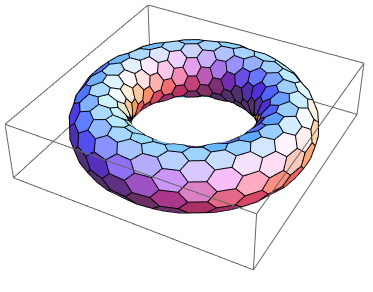
\includegraphics[width=0.75\textwidth]{images/test_image}
	\caption{Cut-Away of Stellarator Reactor} ~\\
\end{figure}

Optimistically, expanding this model would just involve developing a new confinement time scaling law and replacing the Greenwald density limit. The reason the Greenwald density limit is no longer important is because stability is much easier to maintain in a stellarator. Most likely, the density limit will now be governed by Bremsstrahlung radiation. If this were the case, each equation would need to be redivided using it. Ladon would be the reactor built using this enhancement.

\section{Making a Hybrid Reactor -- Janus}

The next interesting reactor would be a hybrid tokamak incorporating pulsed and steady-state operation, codenamed: Janus. Fundamentally, this would mean current would come from both LHCD (steady-state) and inductive (pulsed) sources. This was actually used in Demo Pulsed, but the current drive was not handled self-consistently. Coupling these two current sources could reduce reliance on bootstrap current and lead to much more compact machines.

\begin{figure}
	\centering
	\begin{adjustbox}{width=0.75\textwidth}
		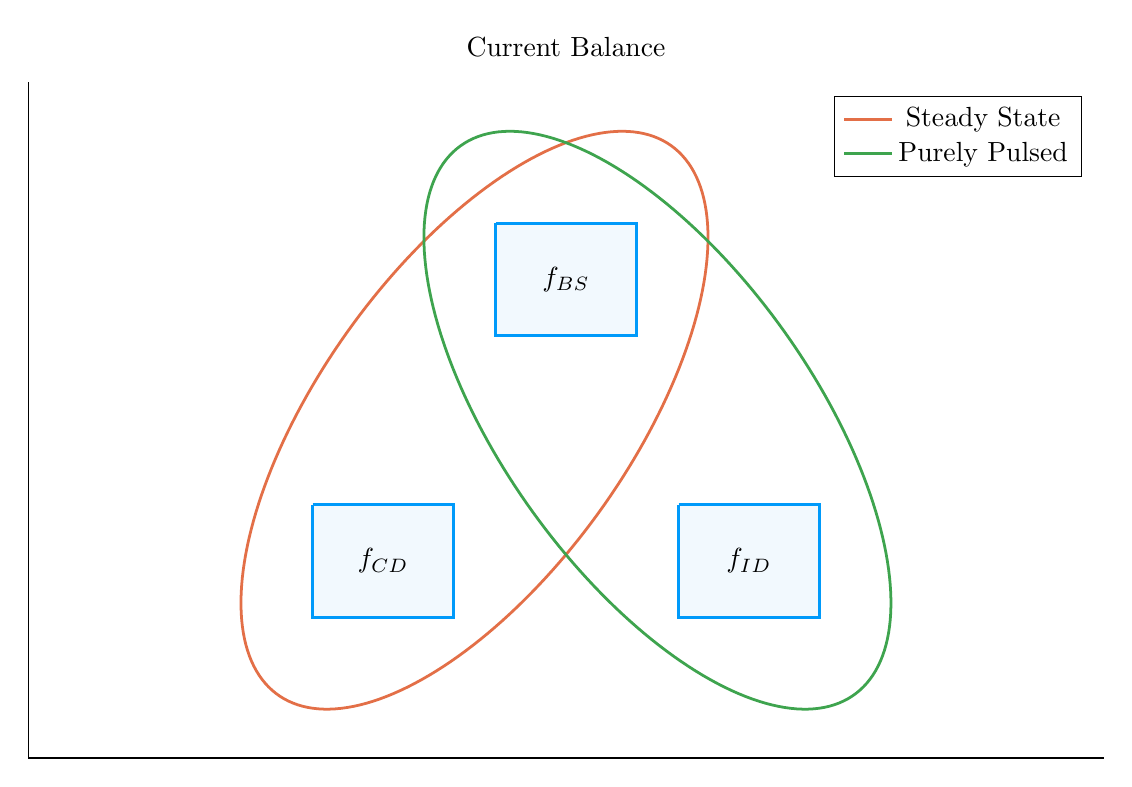
\begin{tikzpicture}[]
\begin{axis}[height = {101.6mm}, axis equal = {true}, ylabel = {}, title = {Current Balance}, xmin = {-5.773116112756781}, xmax = {5.773116112756781}, ymax = {6}, xlabel = {}, {unbounded coords=jump, scaled x ticks = false, xticklabel style={rotate = 0}, xmajorticks=false, xmajorgrids = false, axis lines* = left, scaled y ticks = false, yticklabel style={rotate = 0}, ymajorticks=false, ymajorgrids = false, axis lines* = left,     xshift = 0.0mm,
    yshift = 0.0mm,
    axis background/.style={fill={rgb,1:red,1.00000000;green,1.00000000;blue,1.00000000}}
}, ymin = {-6}, width = {152.4mm}]\addplot+ [color = {rgb,1:red,0.00000000;green,0.60560316;blue,0.97868012},
draw opacity=1.0,
line width=1,
solid,mark = none,
mark size = 2.0,
mark options = {
    color = {rgb,1:red,0.00000000;green,0.00000000;blue,0.00000000}, draw opacity = 1.0,
    fill = {rgb,1:red,0.00000000;green,0.60560316;blue,0.97868012}, fill opacity = 1.0,
    line width = 1,
    rotate = 0,
    solid
},fill = {rgb,1:red,0.00000000;green,0.60560316;blue,0.97868012}, fill opacity=0.05,forget plot]coordinates {
(-1.25, 3.5)
(1.25, 3.5)
(1.25, 1.5)
(-1.25, 1.5)
(-1.25, 3.5)
};
\addplot+ [color = {rgb,1:red,0.00000000;green,0.60560316;blue,0.97868012},
draw opacity=1.0,
line width=1,
solid,mark = none,
mark size = 2.0,
mark options = {
    color = {rgb,1:red,0.00000000;green,0.00000000;blue,0.00000000}, draw opacity = 1.0,
    fill = {rgb,1:red,0.00000000;green,0.60560316;blue,0.97868012}, fill opacity = 1.0,
    line width = 1,
    rotate = 0,
    solid
},fill = {rgb,1:red,0.00000000;green,0.60560316;blue,0.97868012}, fill opacity=0.05,forget plot]coordinates {
(-4.5, -1.5)
(-2.0, -1.5)
(-2.0, -3.5)
(-4.5, -3.5)
(-4.5, -1.5)
};
\addplot+ [color = {rgb,1:red,0.00000000;green,0.60560316;blue,0.97868012},
draw opacity=1.0,
line width=1,
solid,mark = none,
mark size = 2.0,
mark options = {
    color = {rgb,1:red,0.00000000;green,0.00000000;blue,0.00000000}, draw opacity = 1.0,
    fill = {rgb,1:red,0.00000000;green,0.60560316;blue,0.97868012}, fill opacity = 1.0,
    line width = 1,
    rotate = 0,
    solid
},fill = {rgb,1:red,0.00000000;green,0.60560316;blue,0.97868012}, fill opacity=0.05,forget plot]coordinates {
(2.0, -1.5)
(4.5, -1.5)
(4.5, -3.5)
(2.0, -3.5)
(2.0, -1.5)
};
\addplot+ [color = {rgb,1:red,0.88887350;green,0.43564919;blue,0.27812294},
draw opacity=1.0,
line width=1,
solid,mark = none,
mark size = 2.0,
mark options = {
    color = {rgb,1:red,0.00000000;green,0.00000000;blue,0.00000000}, draw opacity = 1.0,
    fill = {rgb,1:red,0.88887350;green,0.43564919;blue,0.27812294}, fill opacity = 1.0,
    line width = 1,
    rotate = 0,
    solid
}]coordinates {
(1.8698661812068136, 4.877080107549691)
(1.7975582266118808, 4.9252162522328415)
(1.7218385915440537, 4.9684428342438745)
(1.6427827549822935, 5.006716764385765)
(1.5604695215037632, 5.03999989037258)
(1.4749809427297138, 5.068259034860505)
(1.3864022355346433, 5.091466028519745)
(1.2948216971002622, 5.109597738114323)
(1.2003306168989445, 5.122636089561793)
(1.1030231856943935, 5.130568085949879)
(1.0029964016502424, 5.133385820492077)
(0.9003499736401737, 5.131086484409318)
(0.7951862218559462, 5.123672369729815)
(0.6876099758124048, 5.111150867004319)
(0.5777284698511354, 5.093534457939059)
(0.46565123624694493, 5.07084070295371)
(0.35148999602370634, 5.043092223676775)
(0.23535854758841435, 5.010316680395862)
(0.11737265329445545, 4.972546744485303)
(-0.00235007595282255, 4.929820065838624)
(-0.12369029793321751, 4.882179235338303)
(-0.2465270580745944, 4.829671742400261)
(-0.37073791002303214, 4.77234992763537)
(-0.49619903770001583, 4.710270930675205)
(-0.6227853787249911, 4.643496633214007)
(-0.7503707490802689, 4.572093597323671)
(-0.878827968893996, 4.496132999103221)
(-1.0080289892158198, 4.415690557728926)
(-1.137845019658864, 4.330846459975782)
(-1.26814665678079, 4.241685280285592)
(-1.3988040130759585, 4.148295896461316)
(-1.5296868464501256, 4.050771401071749)
(-1.6606646900485882, 3.949209008654826)
(-1.7916069823083864, 3.8437099588120507)
(-1.9223831971049103, 3.734379415290662)
(-2.0528629738631725, 3.6213263611541278)
(-2.1829162475040724, 3.5046634901454468)
(-2.3124133780960925, 3.3845070943515854)
(-2.4412252800831986, 3.26097694828099)
(-2.5692235509601344, 3.1341961894697543)
(-2.696280599266827, 3.004291195735447)
(-2.822269771774333, 2.8713914592009493)
(-2.947065479735527, 2.735629457213896)
(-3.0705433240746993, 2.597140520290374)
(-3.192580219391261, 2.4560626972145165)
(-3.3130545166539442, 2.3125366174284774)
(-3.4318461244632026, 2.166705350849943)
(-3.5488366287609345, 2.0187142652569277)
(-3.6639094108681878, 1.8687108813820061)
(-3.776949763733194, 1.7168447258604496)
(-3.8878450062738565, 1.5632671821788118)
(-3.9964845957006974, 1.4081313397725874)
(-4.1027602377083205, 1.2515918414233274)
(-4.206565994425528, 1.0938047291073505)
(-4.307798390016492, 0.9349272884497156)
(-4.4063565138277205, 0.7751178919384804)
(-4.502142120977991, 0.614535841055565)
(-4.595059730290983, 0.4533412074815748)
(-4.685016719472996, 0.29169467353285894)
(-4.771923417440856, 0.12975737198989234)
(-4.8556931937080146, -0.032309274523392384)
(-4.936242544739693, -0.1943437144491822)
(-5.013491177191022, -0.3561844283338884)
(-5.087362087945198, -0.5176700898342566)
(-5.157781640871865, -0.6786397265309694)
(-5.224679640229201, -0.8389328803894542)
(-5.287989400636577, -0.9983897677079463)
(-5.347647813547976, -1.1568514383933535)
(-5.403595410159981, -1.3141599344061687)
(-5.455776420691558, -1.4701584472164726)
(-5.504138829976595, -1.6246914741140965)
(-5.548634429313749, -1.7776049732170973)
(-5.589218864521925, -1.9287465170240605)
(-5.625851680153492, -2.0779654443571474)
(-5.658496359821148, -2.225113010544426)
(-5.687120362598258, -2.3700425356918093)
(-5.711695155456349, -2.5126095508967543)
(-5.732196241707455, -2.6526719422580065)
(-5.74860318542295, -2.7900900925378296)
(-5.760899631804527, -2.9247270203354994)
(-5.769073323487013, -3.0564485166333526)
(-5.773116112756781, -3.1851232785792454)
(-5.773023969673565, -3.3106230403720964)
(-5.768796986087595, -3.432822701120024)
(-5.760439375548035, -3.551600449543642)
(-5.747959469102832, -3.6668378854001826)
(-5.731369706994138, -3.778420137507439)
(-5.710686626257609, -3.8862359782498594)
(-5.685930844237935, -3.9901779344526522)
(-5.657127038037011, -4.090142394513381)
(-5.624303919915274, -4.186029711684261)
(-5.587494208670695, -4.2777443034022165)
(-5.546734597023965, -4.365194746567642)
(-5.502065715042401, -4.448293868676952)
(-5.453532089639006, -4.526958834718015)
(-5.4011821001870715, -4.601111229741906)
(-5.345067930294576, -4.67067713702862)
(-5.285245515786418, -4.735587211768881)
(-5.221774488946376, -4.795776750188546)
(-5.154718119074351, -4.851185754046737)
(-5.084143249418149, -4.901758990443393)
(-5.010120230542682, -4.947446046876624)
(-4.932722850202994, -4.98820138149499)
(-4.852028259791015, -5.023984368494613)
(-4.768116897429388, -5.054759338615853)
(-4.681072407788987, -5.080495614699213)
(-4.590981558710103, -5.101167542264987)
(-4.497934154710361, -5.116754515086211)
(-4.40202294746563, -5.127240995729401)
(-4.303343543353135, -5.132616531042591)
(-4.201994308148942, -5.132875762575277)
(-4.098076268974807, -5.1280184319198305)
(-3.9916930135921564, -5.118049380969083)
(-3.88295058714354, -5.102978547089826)
(-3.7719573864445346, -5.082820953217027)
(-3.658824051931438, -5.0575966928786364)
(-3.543663357372476, -5.02733091016593)
(-3.4265900974524626, -4.9920537746693245)
(-3.3077209733429527, -4.951800451404678)
(-3.1871744763719843, -4.906611065760036)
(-3.065070769909341, -4.8565306634977725)
(-2.941531569585093, -4.801609165851993)
(-2.816680021960811, -4.741901319765965)
(-2.690640581774395, -4.677466643319172)
(-2.5635388878808865, -4.608369366398399)
(-2.435501638012921, -4.5346783666719865)
(-2.306656462485676, -4.456467100931064)
(-2.1771317969721977, -4.373813531866238)
(-2.047056754475925, -4.286800050352669)
(-1.9165609966280504, -4.1955133933210735)
(-1.785774604437966, -4.100044557296444)
(-1.654827948625708, -4.00048870769076)
(-1.523851559665576, -3.896945083940012)
(-1.3929759976705065, -3.7895169005801836)
(-1.26233172224694, -3.678311244360763)
(-1.132048962449818, -3.5634389674983264)
(-1.0022575869674537, -3.4450145771766545)
(-0.8730869746655892, -3.323156121403477)
(-0.7446658856197179, -3.1979850713376368)
(-0.6171223327642645, -3.069626200204022)
(-0.49058345428648176, -2.938207458916877)
(-0.3651753868923626, -2.803859848535569)
(-0.24102314007082093, -2.666717289679875)
(-0.11825047148150092, -2.526916489034983)
(0.0030202364095237577, -2.384596803079324)
(0.12266809832327996, -2.2399000991709683)
(0.2405738466689491, -2.09297061413119)
(0.3566199504324037, -1.9439548104660527)
(0.4706907323336891, -1.7930012303693847)
(0.5826724841366269, -1.6402603476527216)
(0.6924535799956866, -1.4858844177497015)
(0.7999245877270309, -1.3300273259445707)
(0.9049783778929097, -1.1728444339759707)
(1.0075102305906167, -1.0144924251689658)
(1.1074179398395505, -0.8551291482497284)
(1.20460191546238, -0.6949134599984598)
(1.2989652823586764, -0.534005066897528)
(1.3904139770721349, -0.3725643659325606)
(1.478856841555075, -0.210752284705227)
(1.564205714036751, -0.04873012101713625)
(1.6463755169049392, 0.11334061791535466)
(1.725284341513138, 0.27529837645501054)
(1.8008535298288972, 0.4369817115859278)
(1.8730077528418523, 0.598229453843409)
(1.9416750856533156, 0.7588808679712085)
(2.0067870791725912, 0.9187758131459416)
(2.0682788283485025, 1.0777549026089095)
(2.126089036868173, 1.2356596625463219)
(2.1801600782585133, 1.3923326900594108)
(2.2304380533295443, 1.5476178100670777)
(2.2768728439022907, 1.7013602309846187)
(2.3194181627676604, 1.8534066990233193)
(2.358031599826549, 2.0036056509571933)
(2.392674664365143, 2.1518073652044736)
(2.423312823423304, 2.2978641110733555)
(2.4499155362177776, 2.4416302960231726)
(2.4724562845859026, 2.5829626107941834)
(2.490912599419497, 2.7217201722613846)
(2.505266083062553, 2.857764663869852)
(2.5155024276504205, 2.990960473511697)
(2.521611429372199, 3.12117482870718)
(2.5235869986421147, 3.2482779289551793)
(2.5214271661697554, 3.3721430751211794)
(2.515134084923101, 3.4926467957337035)
(2.5047140279823985, 3.609668970063368)
(2.4901773822870172, 3.7230929478618506)
(2.471538638281525, 3.8328056656413696)
(2.448816375471295, 3.9386977593788552)
(2.422033243902053, 4.040663673532358)
(2.391215941581816, 4.1386017662611385)
(2.356395187867742, 4.232414410744436)
(2.317605692844403, 4.322008092498024)
(2.274886122724018, 4.4072935025914814)
(2.2282790613031342, 4.488185626673267)
(2.1778309675141685, 4.564603829714885)
(2.123592129114139, 4.636471936389625)
(2.06561661255673, 4.70371830700579)
(2.0039622090976756, 4.766275908918702)
(1.9386903771871857, 4.824082383350291)
(1.869866181206814, 4.877080107549691)
};
\addlegendentry{Steady State}
\addplot+ [color = {rgb,1:red,0.24222430;green,0.64327509;blue,0.30444865},
draw opacity=1.0,
line width=1,
solid,mark = none,
mark size = 2.0,
mark options = {
    color = {rgb,1:red,0.00000000;green,0.00000000;blue,0.00000000}, draw opacity = 1.0,
    fill = {rgb,1:red,0.24222430;green,0.64327509;blue,0.30444865}, fill opacity = 1.0,
    line width = 1,
    rotate = 0,
    solid
}]coordinates {
(-1.8698661812068136, 4.877080107549691)
(-1.7975582266118808, 4.9252162522328415)
(-1.7218385915440537, 4.9684428342438745)
(-1.6427827549822935, 5.006716764385765)
(-1.5604695215037632, 5.03999989037258)
(-1.4749809427297138, 5.068259034860505)
(-1.3864022355346433, 5.091466028519745)
(-1.2948216971002622, 5.109597738114323)
(-1.2003306168989445, 5.122636089561793)
(-1.1030231856943935, 5.130568085949879)
(-1.0029964016502424, 5.133385820492077)
(-0.9003499736401737, 5.131086484409318)
(-0.7951862218559462, 5.123672369729815)
(-0.6876099758124048, 5.111150867004319)
(-0.5777284698511354, 5.093534457939059)
(-0.46565123624694493, 5.07084070295371)
(-0.35148999602370634, 5.043092223676775)
(-0.23535854758841435, 5.010316680395862)
(-0.11737265329445545, 4.972546744485303)
(0.00235007595282255, 4.929820065838624)
(0.12369029793321751, 4.882179235338303)
(0.2465270580745944, 4.829671742400261)
(0.37073791002303214, 4.77234992763537)
(0.49619903770001583, 4.710270930675205)
(0.6227853787249911, 4.643496633214007)
(0.7503707490802689, 4.572093597323671)
(0.878827968893996, 4.496132999103221)
(1.0080289892158198, 4.415690557728926)
(1.137845019658864, 4.330846459975782)
(1.26814665678079, 4.241685280285592)
(1.3988040130759585, 4.148295896461316)
(1.5296868464501256, 4.050771401071749)
(1.6606646900485882, 3.949209008654826)
(1.7916069823083864, 3.8437099588120507)
(1.9223831971049103, 3.734379415290662)
(2.0528629738631725, 3.6213263611541278)
(2.1829162475040724, 3.5046634901454468)
(2.3124133780960925, 3.3845070943515854)
(2.4412252800831986, 3.26097694828099)
(2.5692235509601344, 3.1341961894697543)
(2.696280599266827, 3.004291195735447)
(2.822269771774333, 2.8713914592009493)
(2.947065479735527, 2.735629457213896)
(3.0705433240746993, 2.597140520290374)
(3.192580219391261, 2.4560626972145165)
(3.3130545166539442, 2.3125366174284774)
(3.4318461244632026, 2.166705350849943)
(3.5488366287609345, 2.0187142652569277)
(3.6639094108681878, 1.8687108813820061)
(3.776949763733194, 1.7168447258604496)
(3.8878450062738565, 1.5632671821788118)
(3.9964845957006974, 1.4081313397725874)
(4.1027602377083205, 1.2515918414233274)
(4.206565994425528, 1.0938047291073505)
(4.307798390016492, 0.9349272884497156)
(4.4063565138277205, 0.7751178919384804)
(4.502142120977991, 0.614535841055565)
(4.595059730290983, 0.4533412074815748)
(4.685016719472996, 0.29169467353285894)
(4.771923417440856, 0.12975737198989234)
(4.8556931937080146, -0.032309274523392384)
(4.936242544739693, -0.1943437144491822)
(5.013491177191022, -0.3561844283338884)
(5.087362087945198, -0.5176700898342566)
(5.157781640871865, -0.6786397265309694)
(5.224679640229201, -0.8389328803894542)
(5.287989400636577, -0.9983897677079463)
(5.347647813547976, -1.1568514383933535)
(5.403595410159981, -1.3141599344061687)
(5.455776420691558, -1.4701584472164726)
(5.504138829976595, -1.6246914741140965)
(5.548634429313749, -1.7776049732170973)
(5.589218864521925, -1.9287465170240605)
(5.625851680153492, -2.0779654443571474)
(5.658496359821148, -2.225113010544426)
(5.687120362598258, -2.3700425356918093)
(5.711695155456349, -2.5126095508967543)
(5.732196241707455, -2.6526719422580065)
(5.74860318542295, -2.7900900925378296)
(5.760899631804527, -2.9247270203354994)
(5.769073323487013, -3.0564485166333526)
(5.773116112756781, -3.1851232785792454)
(5.773023969673565, -3.3106230403720964)
(5.768796986087595, -3.432822701120024)
(5.760439375548035, -3.551600449543642)
(5.747959469102832, -3.6668378854001826)
(5.731369706994138, -3.778420137507439)
(5.710686626257609, -3.8862359782498594)
(5.685930844237935, -3.9901779344526522)
(5.657127038037011, -4.090142394513381)
(5.624303919915274, -4.186029711684261)
(5.587494208670695, -4.2777443034022165)
(5.546734597023965, -4.365194746567642)
(5.502065715042401, -4.448293868676952)
(5.453532089639006, -4.526958834718015)
(5.4011821001870715, -4.601111229741906)
(5.345067930294576, -4.67067713702862)
(5.285245515786418, -4.735587211768881)
(5.221774488946376, -4.795776750188546)
(5.154718119074351, -4.851185754046737)
(5.084143249418149, -4.901758990443393)
(5.010120230542682, -4.947446046876624)
(4.932722850202994, -4.98820138149499)
(4.852028259791015, -5.023984368494613)
(4.768116897429388, -5.054759338615853)
(4.681072407788987, -5.080495614699213)
(4.590981558710103, -5.101167542264987)
(4.497934154710361, -5.116754515086211)
(4.40202294746563, -5.127240995729401)
(4.303343543353135, -5.132616531042591)
(4.201994308148942, -5.132875762575277)
(4.098076268974807, -5.1280184319198305)
(3.9916930135921564, -5.118049380969083)
(3.88295058714354, -5.102978547089826)
(3.7719573864445346, -5.082820953217027)
(3.658824051931438, -5.0575966928786364)
(3.543663357372476, -5.02733091016593)
(3.4265900974524626, -4.9920537746693245)
(3.3077209733429527, -4.951800451404678)
(3.1871744763719843, -4.906611065760036)
(3.065070769909341, -4.8565306634977725)
(2.941531569585093, -4.801609165851993)
(2.816680021960811, -4.741901319765965)
(2.690640581774395, -4.677466643319172)
(2.5635388878808865, -4.608369366398399)
(2.435501638012921, -4.5346783666719865)
(2.306656462485676, -4.456467100931064)
(2.1771317969721977, -4.373813531866238)
(2.047056754475925, -4.286800050352669)
(1.9165609966280504, -4.1955133933210735)
(1.785774604437966, -4.100044557296444)
(1.654827948625708, -4.00048870769076)
(1.523851559665576, -3.896945083940012)
(1.3929759976705065, -3.7895169005801836)
(1.26233172224694, -3.678311244360763)
(1.132048962449818, -3.5634389674983264)
(1.0022575869674537, -3.4450145771766545)
(0.8730869746655892, -3.323156121403477)
(0.7446658856197179, -3.1979850713376368)
(0.6171223327642645, -3.069626200204022)
(0.49058345428648176, -2.938207458916877)
(0.3651753868923626, -2.803859848535569)
(0.24102314007082093, -2.666717289679875)
(0.11825047148150092, -2.526916489034983)
(-0.0030202364095237577, -2.384596803079324)
(-0.12266809832327996, -2.2399000991709683)
(-0.2405738466689491, -2.09297061413119)
(-0.3566199504324037, -1.9439548104660527)
(-0.4706907323336891, -1.7930012303693847)
(-0.5826724841366269, -1.6402603476527216)
(-0.6924535799956866, -1.4858844177497015)
(-0.7999245877270309, -1.3300273259445707)
(-0.9049783778929097, -1.1728444339759707)
(-1.0075102305906167, -1.0144924251689658)
(-1.1074179398395505, -0.8551291482497284)
(-1.20460191546238, -0.6949134599984598)
(-1.2989652823586764, -0.534005066897528)
(-1.3904139770721349, -0.3725643659325606)
(-1.478856841555075, -0.210752284705227)
(-1.564205714036751, -0.04873012101713625)
(-1.6463755169049392, 0.11334061791535466)
(-1.725284341513138, 0.27529837645501054)
(-1.8008535298288972, 0.4369817115859278)
(-1.8730077528418523, 0.598229453843409)
(-1.9416750856533156, 0.7588808679712085)
(-2.0067870791725912, 0.9187758131459416)
(-2.0682788283485025, 1.0777549026089095)
(-2.126089036868173, 1.2356596625463219)
(-2.1801600782585133, 1.3923326900594108)
(-2.2304380533295443, 1.5476178100670777)
(-2.2768728439022907, 1.7013602309846187)
(-2.3194181627676604, 1.8534066990233193)
(-2.358031599826549, 2.0036056509571933)
(-2.392674664365143, 2.1518073652044736)
(-2.423312823423304, 2.2978641110733555)
(-2.4499155362177776, 2.4416302960231726)
(-2.4724562845859026, 2.5829626107941834)
(-2.490912599419497, 2.7217201722613846)
(-2.505266083062553, 2.857764663869852)
(-2.5155024276504205, 2.990960473511697)
(-2.521611429372199, 3.12117482870718)
(-2.5235869986421147, 3.2482779289551793)
(-2.5214271661697554, 3.3721430751211794)
(-2.515134084923101, 3.4926467957337035)
(-2.5047140279823985, 3.609668970063368)
(-2.4901773822870172, 3.7230929478618506)
(-2.471538638281525, 3.8328056656413696)
(-2.448816375471295, 3.9386977593788552)
(-2.422033243902053, 4.040663673532358)
(-2.391215941581816, 4.1386017662611385)
(-2.356395187867742, 4.232414410744436)
(-2.317605692844403, 4.322008092498024)
(-2.274886122724018, 4.4072935025914814)
(-2.2282790613031342, 4.488185626673267)
(-2.1778309675141685, 4.564603829714885)
(-2.123592129114139, 4.636471936389625)
(-2.06561661255673, 4.70371830700579)
(-2.0039622090976756, 4.766275908918702)
(-1.9386903771871857, 4.824082383350291)
(-1.869866181206814, 4.877080107549691)
};
\addlegendentry{Purely Pulsed}
\node at (axis cs:0, 2.5) [,
color={rgb,1:red,0.00000000;green,0.00000000;blue,0.00000000}, draw opacity=1.0,
rotate=0.0
] {$f_{BS}$};
\node at (axis cs:-3.25, -2.5) [,
color={rgb,1:red,0.00000000;green,0.00000000;blue,0.00000000}, draw opacity=1.0,
rotate=0.0
] {$f_{CD}$};
\node at (axis cs:3.25, -2.5) [,
color={rgb,1:red,0.00000000;green,0.00000000;blue,0.00000000}, draw opacity=1.0,
rotate=0.0
] {$f_{ID}$};
\end{axis}

\end{tikzpicture}

	\end{adjustbox}
%	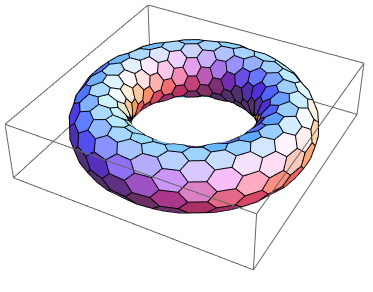
\includegraphics[width=0.75\textwidth]{images/test_image}
	\caption{Current Balance in a Tokamak} ~\\
	\small In a tokamak, there needs to be a certain amount of current -- and that current has to come from somewhere. All good reactors have an adequate bootstrap current. What provides the remaining current is what distinguishes steady state from pulsed operation.
\end{figure}

The arguments against this are mainly technical: why build two difficult auxiliary systems when one is needed -- especially when they probably work against each other. Although rational, the argument implicitly assumes a current is achievable through only one source (i.e. either through LHCD or from a central solenoid). Using two may allow for larger plasma currents.

\section{Bridging Confinement Scalings -- Daedalus}

The final potential reactor -- Daedalus -- is designed to colelct as many scaling laws as possible. As a baseline, it should be able to run in H-Mode, L-Mode, and I-Mode. Because L-Mode is available on any machine, the first step is building under H-Mode. The goal then is to find reactors that can also reach I-Mode -- thus improving the scaling law's fit and making the  actual reactor more cost effective.

Repeated below are the three confinement scaling laws, as well as the generalized formula. As should be noted, the I-Mode scaling currently lacks a true radial dependence -- as it has only been found on two machines. This is one reason Daedalus would be so valuable.

\begin{equation}
  \tau_E^G = K_\tau \, H \, \frac{
    I_P^{\,\alpha_I} \, R_0^{\,\alpha_R} \, a^{\,\alpha_a} \, \kappa^{\,\alpha_\kappa} \ \overline{n}^{\,\alpha_n} \, B_0^{\,\alpha_B} \, A^{\,\alpha_A}
  }{ P_L ^ {\,\alpha_P} }
  \tag{\ref{eq:tau_gen}}
\end{equation}

\begin{equation}
  \tau_E^H = 0.145 \, H \, \frac{
    I_P^{0.93} \, R_0^{1.39} \, a^{0.58} \, \kappa^{0.78} \ \overline{n}^{\, 0.41} \, B_0^{0.15} \, A^{0.19}
  }{ P_L ^ {\,0.69} }
  \tag{\ref{eq:tau_h}}
\end{equation}

\begin{equation}
  \tau_E^L = 0.048\, H \, \frac{
    I_P^{0.85} \, R_0^{1.2} \, a^{0.3} \, \kappa^{0.5} \ \overline{n}^{\, 0.1} \, B_0^{0.2} \, A^{0.5} }{ P_L ^ {\,0.5} }
\end{equation}

\begin{equation}
  \tau_E^I = \frac{ 0.014 \, H }{ 0.68 ^ {\lambda_R} \cdot 0.22 ^ {\lambda_a} } \cdot \frac{ I_P^{0.69} \, R_0^{\lambda_R} \, a^{\lambda_a} \, \kappa^{0.0} \ \overline{n}^{\, 0.17} \, B_0^{0.77} \, A^{0.0} }{ P_L ^ {\,0.29} }
\end{equation}

\begin{equation}
	\lambda_R + \lambda_a = 2.2
\end{equation}

Before moving on, it is important to reemphasize that the I-Mode scaling law is not battle-tested . It is the target of ongoing research at the MIT PSFC.


%\end{document}
